% !TeX root = scaffold-40.tex
\renewcommand{\imagepath}{../40-coils/img}

\chapter{Feshbach and Gradient Field Coils}\label{ch:coils}
This chapter treats of the coils used for generating homogeneous magnetic fields for tuning Feshbach resonances and for creating magnetic gradients for the three-dimensional magneto-optical trap: First, it is outlined which requirements and constraints these coils are subject to in the experiment. Then a Python library developed for simulating magnetic fields and operational properties of coil arrangements is presented. Afterwards, the coils and the magnetic fields are characterized with measurements and simulations. In this chapter, these coils are called \textit{Feshbach coils}.

\section{Requirements and Constraints}
The FermiQP demonstrator setup and its planned experimental operations impose certain requirements and constraints on the fields as well as the design  and the geometry of the Feshbach coils:

\subsection*{Magnetic Field Strength}
The Feshbach coils serve two main purposes: On the one hand, they produce strong homogeneous magnetic fields, e.g. for scanning over the Feshbach resonance of lithium at \SI{834}{\gauss} and thereby tuning on-site interactions in the Fermi-Hubbard model, as described in chapter~\ref{ch:analog_mode}. On the other hand, they provide magnetic gradients up to the order of \SI[]{e2}{\gauss\per\centi\meter} for the three-dimensional magneto optical trap. A value of \SI{1300}{\gauss} was set as the target field magnitude in the homogeneous mode, created at a current of $I = \SI{400}{\ampere}$ provided by two high-current power supplies for each coil\footnote{Delta Elektronika SM 15-400 with a maximum output power of \SI[]{6}{\kilo\watt}, voltage up to \SI[]{15}{\volt}, and current up to \SI[]{400}{\ampere}}.

In order to generate flat homogeneous fields, the coils are arranged in Helmholtz configuration, meaning that two equally-sized circular coils are placed on a common axis such that their distance is equal to their radius.\footnote{In the rest of this chapter, the term \textit{Helmholtz configuration} will refer to two coils of the same size sharing the same axis at a distance equal to their radii. All coil arrangements discussed in this chapter will be in Helmholtz configuration. If the current in both coils flows in the same direction, meaning that the coils generate a homogeneous field between them, the operation mode will be referred to as \textit{homogeneous field mode}. If, however, the current flows in opposite directions such that the coils generate a field gradient between them, the operation mode will be referred to as \textit{gradient mode}. Note that, similar to the $d = r$ condition of the Helmholtz configuration, there is a different optimal configuration for gradient fields, often called \textit{anti-Helmholtz configuration}, which however requires a different distance $d \neq r$ and does not occur in this chapter.} The effective optimal ratio of distance and radius required, however, depends on the finite size and the actual geometry of the coils.

\subsection*{Geometry}
In order to produce these strong fields with reasonable currents, the radius of the coils should be kept as small as possible, and they should be placed as close to the glass cell as possible.

The coils will enclose the two objectives above and below the glass cell between them. This introduces a minimum distance of around \SI{50}{\milli\meter} between the coils still allowing a few \si[]{\milli\meter} of leeway to fit the objectives between the coils. It was decided for a distance of \SI{55}{\milli\meter} between the innermost wires of the coils, not considering additional surface material on the coils. These geometrical constraints led to the estimation that 30 windings are needed to attain the required \SI{1300}{\gauss} of field\footnote{Estimated using simulations  as outlined in sections~\ref{ch:simulation} and~\ref{ch:coil_properties}}.

The orientation of the coil arrangement is constrained by the requirement that Raman transitions on the atoms in the optical lattice be driven with $\pi$-polarized light shone in through the objectives. As this light propagates along the $z$ axis, its polarization vector lies in the $xy$ plane. Since $\pi$ transitions can only be driven if the polarization vector and the quantization axis are parallel, the direction of the magnetic field and hence also the coil axis are constrained to the $xy$ plane. It was decided to align the coil arrangement with the $y$ axis, meaning that the two coils sit on the left and on the right of the glass cell with the coil axis passing through the trap region of the magneto-optical trap.

Figure~\ref{fig:feshbach_coil_geometry_constraints} shows the geometrical constraints on the positioning of the coils.

\begin{figure}
    \centering
    \includegraphics[]{\imagepath/feshbach_coil_geometry_constraints/feshbach_coil_geometry_constraints.pdf}
    \caption{Position of the Feshbach coils with respect to the glass cell and the objectives: The objectives (\SI{44}{\milli\meter} diameter) which are positioned below and above the glass cell are enclosed by the two coils, setting the minimum distance between the coils. The innermost coil wires have a distance of \SI{55}{\milli\meter}.}
    \label{fig:feshbach_coil_geometry_constraints}
\end{figure}

Since the coils have many windings and so also a significant size, they block a non-negligible part of the optical access to the location of the atoms in the glass cell. Many laser beams and imaging signals must be shot into and received from the glass cell, demanding that the coils leave open as much solid angle as possible. Most notably, the pinning lattice beams enter through the long surfaces on the left and right with incidence angles of $\pm \SI{45}{\degree}$, the science lattice beams enter with incidence angles of around $\pm \SI{15}{\degree}$ on the short sides of the glass cell bounding the available space for the coils. In order to minimize the blocked optical access, a cone-like coil geometry with a parallelogram-shaped cross-section consisting of $6 \times 5$ windings was opted for, as depicted in figure~\ref{fig:parallelogram_cross_section}. The opening angle of the cone has been set to $\SI{45}{\degree}$ because then the Helmholtz condition is approximately fulfilled for every layer.
\begin{figure}
    \centering
    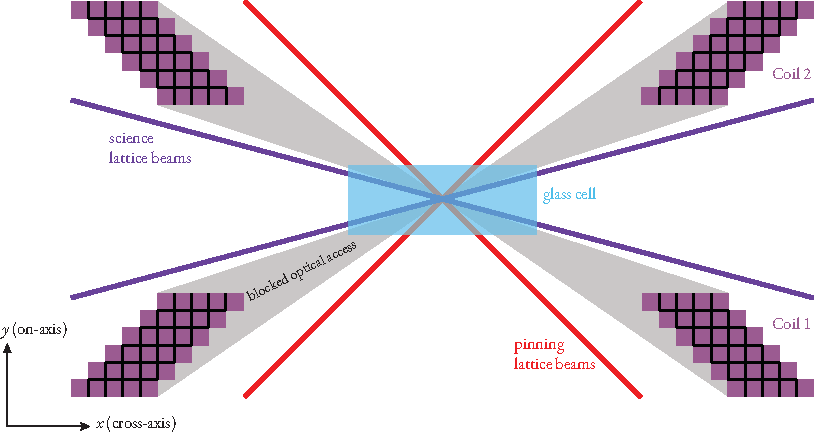
\includegraphics[]{\imagepath/parallelogram_cross_section/parallelogram_cross_section.pdf}
    \caption{Parallelogram-shaped cross-section of the coils for minimizing the blocked optical access into the glass cell, letting the pinning and science lattice beams pass alongside the coil (view from above): The windings layers stacked onto each other (in the coil axis direction) have radii that increase by one wire size per layer (cross-axis direction), corresponding to a cone opening angle of \SI[]{45}{\degree}.}
    \label{fig:parallelogram_cross_section}
\end{figure}

\subsection*{Field and Temperature Stability}
The FermiQP demonstrator aims for a relative field stability of \SI{e-7}{} calling for an active stabilization mechanism. For this purpose, both coils are independently driven by separate power supplies supporting fast current switching.

Furthermore, it is important to ensure thermal stability of the coils. The electrical power $P(I) = RI^2$ dissipated in the coils with resistance $R$ shows quadratic scaling  with the driving current $I$. For an exemplary coil with \SI{10}{\milli\ohm} resistance driven with $I = \SI{400}{\ampere}$ this would amount to a dissipated power of \SI{1.6}{\kilo\watt} converted into heat. In order to transport this heat off efficiently, avoiding a critical increase of temperature, the coils need to feature hollow-core wires for water cooling. For a given maximal temperature increase $\Delta T$ of the cooling water, the cooling power of the water can be estimated as $Q_\text{cool} = c_\text{water} ~ \Delta T ~ m_\text{water} ~ v_\text{flow}$ with the heat capacity $ c_\text{water}$ of water, the specific mass $m_\text{water}$ of the water in the hollow-core wire, and the speed $v_\text{flow}$ of the cooling water flow, which depends on the applied pressure, the turbulence of the flow, and the wire geometry.

To lower the required cooling water pressure and to avoid turbulences in the cooling water stream, it was decided to separate the six wire layers into three pancakes of two layers each, constituting three separately driven water cooling circuits, as shown in figure~\ref{fig:pancake_structure}. The two supply lines for each pancake are placed next to each other, forming pairs of wires with current flowing in opposite directions. This has the additional advantage that the fields of the supply lines cancel out in the far-field and do not influence the magnetic field in the center of the coil arrangement.

\begin{figure}
    \centering
    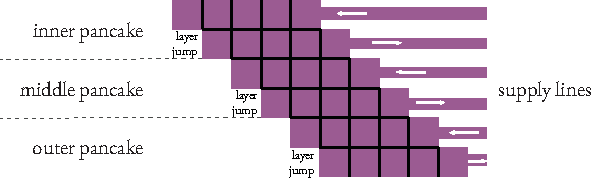
\includegraphics[]{\imagepath/pancake_structure/pancake_structure.pdf}
    \caption{Cross-section of the pancake structure of the coils: Two layers of wire are combined into a so-called pancake that constitutes a single water cooling circuit. The layers have layer jump on the innermost winding where the wire hops from one layer to the other. The current in the two supply lines for each pancake is flowing in opposite directions such that the magnetic fields originating from the wire cancel out in the far-field.}
    \label{fig:pancake_structure}
\end{figure}

\subsection*{Field Curvature}\label{ch:field_curvature_definition}
When the atoms trapped in glass cell are exposed to the homogeneous magnetic field, they experience an energy shift resulting from the interaction of their magnetic moment $\vec \mu$ with the field $\vec B$ which can lead to trapping or anti-trapping effects~\cite{pritchard_cooling_1983,gehm_properties_2003, hagemann_setup_2020}:
\begin{align}
    E_{B, {\text{high-field seeker} \atop \text{low-field seeker}}} = \mp \vec \mu \vec B
\end{align}
where the sign of the shift depends on whether the atoms are in high- or low-field seeking states. The magnitude of the magnetic moment is $\mu \approx \mu_\text{B}$ with the Bohr magneton $\mu_\text{B} = \SI{9.27e-24}{\joule\per\tesla}$.

In the very center of the coil arrangement, the magnetic field is completely homogeneous in case of optimally positioned coils. Realistically, however, there is a non-negligible position dependence $B(\vec r)$ of the field, stemming from the finite size of the region of interest and imperfections in positioning, aligning, and manufacturing of the coils. This leads to a potential landscape that the atoms are exposed to such that their Hamiltonian reads:
\begin{align}
    \hat H(\vec r) = \frac{\vec p^2}{2m} \mp \vec \mu_\text{B} \vec B(\vec r)
\end{align}

Assuming that the magnetic field around the center of the coil arrangement in one dimension follows a paraboloid shape, modelled as $B(q) = B_0 + a_{\vec q} q^2$ with a field curvature coefficient $a$ and a spatial coordinate $q$, one can equate the magnetic potential with that of a quantum mechanical harmonic oscillator:
\begin{align}
    \underbrace{V_0 + \frac{1}{2}m\omega^2q^2}_{V_\text{HO}(q)} ~~~\equiv~~~ \underbrace{\mp \mu_\text{B} B_0 \mp \mu_\text{B} a_{\vec q} q^2}_{V_\text{magnetic}(q)}
\end{align}

Identifying the position-dependent terms, the magnetic potential can be assigned the angular trap frequency $\omega_{\vec q}$ along the $\vec q$ coordinate axis:
\begin{align}\label{eq:trap_omega_definition}
    \omega_{\vec q} = \sqrt[]{\mp\frac{2 \mu_\text{B} a_{\vec q}}{m}}
\end{align}
In the following, the trapping potential is considered trapping in the ${\vec q}$ direction if $\omega_{\vec q}$ is real, and anti-trapping if $\omega_{\vec q}$ is imaginary. For high-field seekers, the potential is trapping if $a_{\vec q} < 0$ and anti-trapping if $a_{\vec q} > 0$, and vice versa for low-field seekers. This can be intuitively seen as high-field seekers are trapped if the field has a maximum and is concave, hence $a_{\vec q} < 0$, and the other way around for low-field seekers.

In a field landscape between two coils, if the potential is trapping along the arrangement axis, it is anti-trapping in the cross-axis directions, and vice versa. This is due to Earnshaw's theorem~\cite{earnshaw_nature_1842} stating that a magnetic field in three dimensions has the shape of a hyperboloid, and thus cannot have a global extremum rather than a saddle point. This implies that the magnetic field is curved into opposite directions along the on-axis and cross-axis directions, as shown in figure~\ref{fig:field_landscape}. The field in the on-axis direction is curved twice as much as in the cross-axis direction: $\frac{a_\text{on-axis}}{a_\text{cross-axis}} = -2$, hence the trap frequencies have a ratio of $\frac{|\omega_\text{on-axis}|}{|\omega_\text{cross-axis}|} = \sqrt{2}$~\cite{hagemann_setup_2020} (see also figure~\ref{fig:feshbach_field_trap_frequencies} in section~\ref{ch:field_characterization}).

Note that $a_{\vec q}$ relates to the field landscape along ${\vec q}$ as $a_{\vec q}  = \frac{1}{2} \pdv[2]{B}{q}$ which can be seen from the Taylor expansion $B(q) = \eval{B}_{0} + \eval{\pdv{B}{q}}_{0} q + \frac{1}{2} \eval{\pdv[2]{B}{q}}_{0} q^2 + \mathcal{O}(q^3)$ around $0$ identifying the second order term with $a_{\vec q} q^2$.

\begin{figure}
    \centering
    \begin{pgfpicture}
        \pgftext{\input{\imagepath/field_landscape/field_landscape.pgf}}
    \end{pgfpicture}
    \caption{Field curvature at the center of a homogeneous field between two coils: While the curvature is positive along one axis (here along $y$, blue, anti-trapping for high-field seekers), it is negative along the other axis (here along $x$, red, trapping for high-field seekers).}
    \label{fig:field_landscape}
\end{figure}

The design goal for the coil arrangement with regard to the field curvature is to minimize the absolute trap frequency in each direction by setting the coil distance accordingly.

\section{Simulation}\label{ch:simulation}
In order to determine the optimal specifications and to characterize the coils, a simulation python library was developed (called \textit{coil simulation library}). It makes heavy use of the magnetic field Python library \textit{magpylib}~\cite{ortner_magpylib_2020, noauthor_magpylibmagpylib_nodate} providing magnetic field vectors at arbitrary positions originating from wire loops, straight wires, and permanent magnets of different shapes only from analytic calculations.

\subsection*{Modelling}
The \textit{coil simulation library} models arrangements of two or more coils sharing a common axis. The models are parameterized by the distance $d_\text{coil}$ of the coils to the center, the number $n_\text{coil}$, the radius $r_\text{coil}$, and the arrangement geometry of the windings of each coil, the spacing $w$ between the windings, and the current $I_\text{coil}$ flowing in each coil and, if desired, even in each winding.

A coil is modelled as a set $\mathcal{C}$ of circular wire loops $L(r, y, I)$ with radius $r$, center position $y$, and current $I$. As is the case for the FermiQP demonstrator, the wire loops are aligned with the $y$ axis. For the $n_\text{on-axis}$ on-axis windings and the $n_\text{cross-axis}$ cross-axis windings ($6$ and $5$ for the FermiQP demonstrator), each loop $L_{ac}$ with on-axis index $a \in \{0, \ldots, n_\text{on-axis} - 1\}$ and cross-axis index $c \in \{0, \ldots n_\text{cross-axis} - 1\}$ is defined as
\begin{align}
    L_{ac} = L \left(r_\text{coil} + r_{ac}, y_\text{coil} + y_{ac}, I_\text{coil}\right)
\end{align}
with the on-axis ($y$) and radial (cross-axis) offsets
\begin{align}
    \label{eq:coil_model_yac}
    y_{ac} &= w\cdot \left(a-\frac{n_\text{on-axis}}{2} + \frac{1}{2}\right) \\
    \label{eq:coil_model_rac}
    r_{ac} &= y_{ac} \tan \eta + w \cdot \left(c - \frac{n_\text{cross-axis}}{2} + \frac{1}{2}\right)
\end{align}
where $w$ is the side length of a wire, and $\eta$ is the opening angle of the parallelogram-shaped cross-section of the coil cone ($\eta = \SI{45}{\degree}$ for the coils in the FermiQP demonstrator). Figure~\ref{fig:coil_model} visualizes how a coil is modelled as a set of wire loops.

This way of modelling a coil neglects the spiral shape of the coil wire as well as the wire jumps between the layers of the coil.

\begin{figure}
    \centering
    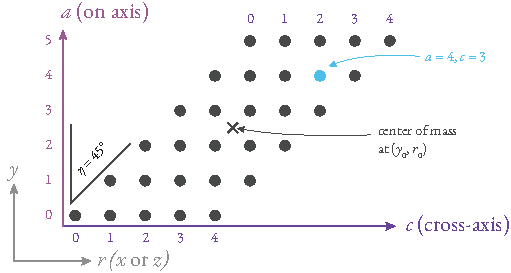
\includegraphics[]{\imagepath/coil_model/coil_model.pdf}
    \caption{A coil is modelled as a set of wire loops with on-axis indices $a$ and cross-axis/radial indices $c$ (counted from $0$), here shown in the cross-section view. The layers along the coil axis enclose an angle $\eta$. In the case of the coils for the FermiQP demonstrator with $6 \times 5$ windings, $a$ corresponds to the $y$ axis, and $c$ corresponds to the radial axes in the $xz$ plane, and the angle $\eta$ is \SI[]{45}{\degree}. The winding $(a = 3, c=2)$ is exemplarily highlighted, according~\eqref{eq:coil_model_yac} and~\eqref{eq:coil_model_rac} it lies at $(y = y_0 + \frac{3}{2}w, r = r_0 + \frac{5}{2}w)$.}
    \label{fig:coil_model}
\end{figure}

For an arrangement, the library provides the user with magnetic field vectors and magnitudes at arbitrary positions, plots of the fields along the arrangement axes, maps of the field landscape in the arrangement, information about gradients and curvatures of the fields, resistances, inductances, dipole moments, $L\over R$ time constants, mutually exerted mechanical forces of the coils, and sketches of the winding geometry (see figure~\ref{fig:csl_sketches} for exemplary sketches for the Feshbach coils).

\begin{figure}
    \centering
    \begin{subfigure}[t]{0.47\textwidth}
        \centering
        \resizebox{\textwidth}{!}{
            \begin{pgfpicture}
                \pgftext{%% Creator: Matplotlib, PGF backend
%%
%% To include the figure in your LaTeX document, write
%%   \input{<filename>.pgf}
%%
%% Make sure the required packages are loaded in your preamble
%%   \usepackage{pgf}
%%
%% Also ensure that all the required font packages are loaded; for instance,
%% the lmodern package is sometimes necessary when using math font.
%%   \usepackage{lmodern}
%%
%% Figures using additional raster images can only be included by \input if
%% they are in the same directory as the main LaTeX file. For loading figures
%% from other directories you can use the `import` package
%%   \usepackage{import}
%%
%% and then include the figures with
%%   \import{<path to file>}{<filename>.pgf}
%%
%% Matplotlib used the following preamble
%%   \usepackage{fontspec}
%%   \setmainfont{DejaVuSerif.ttf}[Path=\detokenize{/home/max/.conda/envs/3d_mot/lib/python3.9/site-packages/matplotlib/mpl-data/fonts/ttf/}]
%%   \setsansfont{DejaVuSans.ttf}[Path=\detokenize{/home/max/.conda/envs/3d_mot/lib/python3.9/site-packages/matplotlib/mpl-data/fonts/ttf/}]
%%   \setmonofont{DejaVuSansMono.ttf}[Path=\detokenize{/home/max/.conda/envs/3d_mot/lib/python3.9/site-packages/matplotlib/mpl-data/fonts/ttf/}]
%%
\begingroup%
\makeatletter%
\begin{pgfpicture}%
\pgfpathrectangle{\pgfpointorigin}{\pgfqpoint{3.956958in}{3.906781in}}%
\pgfusepath{use as bounding box, clip}%
\begin{pgfscope}%
\pgfsetbuttcap%
\pgfsetmiterjoin%
\pgfsetlinewidth{0.000000pt}%
\definecolor{currentstroke}{rgb}{1.000000,1.000000,1.000000}%
\pgfsetstrokecolor{currentstroke}%
\pgfsetstrokeopacity{0.000000}%
\pgfsetdash{}{0pt}%
\pgfpathmoveto{\pgfqpoint{0.000000in}{0.000000in}}%
\pgfpathlineto{\pgfqpoint{3.956958in}{0.000000in}}%
\pgfpathlineto{\pgfqpoint{3.956958in}{3.906781in}}%
\pgfpathlineto{\pgfqpoint{0.000000in}{3.906781in}}%
\pgfpathlineto{\pgfqpoint{0.000000in}{0.000000in}}%
\pgfpathclose%
\pgfusepath{}%
\end{pgfscope}%
\begin{pgfscope}%
\pgfsetbuttcap%
\pgfsetmiterjoin%
\definecolor{currentfill}{rgb}{1.000000,1.000000,1.000000}%
\pgfsetfillcolor{currentfill}%
\pgfsetlinewidth{0.000000pt}%
\definecolor{currentstroke}{rgb}{0.000000,0.000000,0.000000}%
\pgfsetstrokecolor{currentstroke}%
\pgfsetstrokeopacity{0.000000}%
\pgfsetdash{}{0pt}%
\pgfpathmoveto{\pgfqpoint{0.100000in}{0.336624in}}%
\pgfpathlineto{\pgfqpoint{3.570157in}{0.336624in}}%
\pgfpathlineto{\pgfqpoint{3.570157in}{3.806781in}}%
\pgfpathlineto{\pgfqpoint{0.100000in}{3.806781in}}%
\pgfpathlineto{\pgfqpoint{0.100000in}{0.336624in}}%
\pgfpathclose%
\pgfusepath{fill}%
\end{pgfscope}%
\begin{pgfscope}%
\pgfsetbuttcap%
\pgfsetmiterjoin%
\definecolor{currentfill}{rgb}{0.950000,0.950000,0.950000}%
\pgfsetfillcolor{currentfill}%
\pgfsetfillopacity{0.500000}%
\pgfsetlinewidth{1.003750pt}%
\definecolor{currentstroke}{rgb}{0.950000,0.950000,0.950000}%
\pgfsetstrokecolor{currentstroke}%
\pgfsetstrokeopacity{0.500000}%
\pgfsetdash{}{0pt}%
\pgfpathmoveto{\pgfqpoint{0.486416in}{1.046880in}}%
\pgfpathlineto{\pgfqpoint{1.536276in}{1.945748in}}%
\pgfpathlineto{\pgfqpoint{1.517948in}{3.659170in}}%
\pgfpathlineto{\pgfqpoint{0.406029in}{2.856568in}}%
\pgfusepath{stroke,fill}%
\end{pgfscope}%
\begin{pgfscope}%
\pgfsetbuttcap%
\pgfsetmiterjoin%
\definecolor{currentfill}{rgb}{0.900000,0.900000,0.900000}%
\pgfsetfillcolor{currentfill}%
\pgfsetfillopacity{0.500000}%
\pgfsetlinewidth{1.003750pt}%
\definecolor{currentstroke}{rgb}{0.900000,0.900000,0.900000}%
\pgfsetstrokecolor{currentstroke}%
\pgfsetstrokeopacity{0.500000}%
\pgfsetdash{}{0pt}%
\pgfpathmoveto{\pgfqpoint{1.536276in}{1.945748in}}%
\pgfpathlineto{\pgfqpoint{3.230951in}{1.444107in}}%
\pgfpathlineto{\pgfqpoint{3.305917in}{3.212113in}}%
\pgfpathlineto{\pgfqpoint{1.517948in}{3.659170in}}%
\pgfusepath{stroke,fill}%
\end{pgfscope}%
\begin{pgfscope}%
\pgfsetbuttcap%
\pgfsetmiterjoin%
\definecolor{currentfill}{rgb}{0.925000,0.925000,0.925000}%
\pgfsetfillcolor{currentfill}%
\pgfsetfillopacity{0.500000}%
\pgfsetlinewidth{1.003750pt}%
\definecolor{currentstroke}{rgb}{0.925000,0.925000,0.925000}%
\pgfsetstrokecolor{currentstroke}%
\pgfsetstrokeopacity{0.500000}%
\pgfsetdash{}{0pt}%
\pgfpathmoveto{\pgfqpoint{0.486416in}{1.046880in}}%
\pgfpathlineto{\pgfqpoint{2.274422in}{0.457731in}}%
\pgfpathlineto{\pgfqpoint{3.230951in}{1.444107in}}%
\pgfpathlineto{\pgfqpoint{1.536276in}{1.945748in}}%
\pgfusepath{stroke,fill}%
\end{pgfscope}%
\begin{pgfscope}%
\pgfsetrectcap%
\pgfsetroundjoin%
\pgfsetlinewidth{0.803000pt}%
\definecolor{currentstroke}{rgb}{0.000000,0.000000,0.000000}%
\pgfsetstrokecolor{currentstroke}%
\pgfsetdash{}{0pt}%
\pgfpathmoveto{\pgfqpoint{0.486416in}{1.046880in}}%
\pgfpathlineto{\pgfqpoint{2.274422in}{0.457731in}}%
\pgfusepath{stroke}%
\end{pgfscope}%
\begin{pgfscope}%
\definecolor{textcolor}{rgb}{0.000000,0.000000,0.000000}%
\pgfsetstrokecolor{textcolor}%
\pgfsetfillcolor{textcolor}%
\pgftext[x=0.931884in, y=0.263902in, left, base,rotate=341.762949]{\color{textcolor}\rmfamily\fontsize{9.000000}{10.800000}\selectfont x [mm]}%
\end{pgfscope}%
\begin{pgfscope}%
\pgfsetbuttcap%
\pgfsetroundjoin%
\pgfsetlinewidth{0.803000pt}%
\definecolor{currentstroke}{rgb}{0.690196,0.690196,0.690196}%
\pgfsetstrokecolor{currentstroke}%
\pgfsetdash{}{0pt}%
\pgfpathmoveto{\pgfqpoint{0.569447in}{1.019521in}}%
\pgfpathlineto{\pgfqpoint{1.615255in}{1.922370in}}%
\pgfpathlineto{\pgfqpoint{1.601081in}{3.638383in}}%
\pgfusepath{stroke}%
\end{pgfscope}%
\begin{pgfscope}%
\pgfsetbuttcap%
\pgfsetroundjoin%
\pgfsetlinewidth{0.803000pt}%
\definecolor{currentstroke}{rgb}{0.690196,0.690196,0.690196}%
\pgfsetstrokecolor{currentstroke}%
\pgfsetdash{}{0pt}%
\pgfpathmoveto{\pgfqpoint{0.930624in}{0.900513in}}%
\pgfpathlineto{\pgfqpoint{1.958480in}{1.820772in}}%
\pgfpathlineto{\pgfqpoint{1.962585in}{3.547995in}}%
\pgfusepath{stroke}%
\end{pgfscope}%
\begin{pgfscope}%
\pgfsetbuttcap%
\pgfsetroundjoin%
\pgfsetlinewidth{0.803000pt}%
\definecolor{currentstroke}{rgb}{0.690196,0.690196,0.690196}%
\pgfsetstrokecolor{currentstroke}%
\pgfsetdash{}{0pt}%
\pgfpathmoveto{\pgfqpoint{1.299080in}{0.779107in}}%
\pgfpathlineto{\pgfqpoint{2.308089in}{1.717284in}}%
\pgfpathlineto{\pgfqpoint{2.331176in}{3.455833in}}%
\pgfusepath{stroke}%
\end{pgfscope}%
\begin{pgfscope}%
\pgfsetbuttcap%
\pgfsetroundjoin%
\pgfsetlinewidth{0.803000pt}%
\definecolor{currentstroke}{rgb}{0.690196,0.690196,0.690196}%
\pgfsetstrokecolor{currentstroke}%
\pgfsetdash{}{0pt}%
\pgfpathmoveto{\pgfqpoint{1.675037in}{0.655229in}}%
\pgfpathlineto{\pgfqpoint{2.664262in}{1.611853in}}%
\pgfpathlineto{\pgfqpoint{2.707067in}{3.361847in}}%
\pgfusepath{stroke}%
\end{pgfscope}%
\begin{pgfscope}%
\pgfsetbuttcap%
\pgfsetroundjoin%
\pgfsetlinewidth{0.803000pt}%
\definecolor{currentstroke}{rgb}{0.690196,0.690196,0.690196}%
\pgfsetstrokecolor{currentstroke}%
\pgfsetdash{}{0pt}%
\pgfpathmoveto{\pgfqpoint{2.058727in}{0.528803in}}%
\pgfpathlineto{\pgfqpoint{3.027185in}{1.504424in}}%
\pgfpathlineto{\pgfqpoint{3.090475in}{3.265981in}}%
\pgfusepath{stroke}%
\end{pgfscope}%
\begin{pgfscope}%
\pgfsetrectcap%
\pgfsetroundjoin%
\pgfsetlinewidth{0.803000pt}%
\definecolor{currentstroke}{rgb}{0.000000,0.000000,0.000000}%
\pgfsetstrokecolor{currentstroke}%
\pgfsetdash{}{0pt}%
\pgfpathmoveto{\pgfqpoint{0.578493in}{1.027330in}}%
\pgfpathlineto{\pgfqpoint{0.551321in}{1.003872in}}%
\pgfusepath{stroke}%
\end{pgfscope}%
\begin{pgfscope}%
\definecolor{textcolor}{rgb}{0.000000,0.000000,0.000000}%
\pgfsetstrokecolor{textcolor}%
\pgfsetfillcolor{textcolor}%
\pgftext[x=0.475564in,y=0.781193in,,top]{\color{textcolor}\rmfamily\fontsize{9.000000}{10.800000}\selectfont \ensuremath{-}100}%
\end{pgfscope}%
\begin{pgfscope}%
\pgfsetrectcap%
\pgfsetroundjoin%
\pgfsetlinewidth{0.803000pt}%
\definecolor{currentstroke}{rgb}{0.000000,0.000000,0.000000}%
\pgfsetstrokecolor{currentstroke}%
\pgfsetdash{}{0pt}%
\pgfpathmoveto{\pgfqpoint{0.939521in}{0.908478in}}%
\pgfpathlineto{\pgfqpoint{0.912795in}{0.884550in}}%
\pgfusepath{stroke}%
\end{pgfscope}%
\begin{pgfscope}%
\definecolor{textcolor}{rgb}{0.000000,0.000000,0.000000}%
\pgfsetstrokecolor{textcolor}%
\pgfsetfillcolor{textcolor}%
\pgftext[x=0.836684in,y=0.659511in,,top]{\color{textcolor}\rmfamily\fontsize{9.000000}{10.800000}\selectfont \ensuremath{-}50}%
\end{pgfscope}%
\begin{pgfscope}%
\pgfsetrectcap%
\pgfsetroundjoin%
\pgfsetlinewidth{0.803000pt}%
\definecolor{currentstroke}{rgb}{0.000000,0.000000,0.000000}%
\pgfsetstrokecolor{currentstroke}%
\pgfsetdash{}{0pt}%
\pgfpathmoveto{\pgfqpoint{1.307820in}{0.787234in}}%
\pgfpathlineto{\pgfqpoint{1.281564in}{0.762820in}}%
\pgfusepath{stroke}%
\end{pgfscope}%
\begin{pgfscope}%
\definecolor{textcolor}{rgb}{0.000000,0.000000,0.000000}%
\pgfsetstrokecolor{textcolor}%
\pgfsetfillcolor{textcolor}%
\pgftext[x=1.205100in,y=0.535371in,,top]{\color{textcolor}\rmfamily\fontsize{9.000000}{10.800000}\selectfont 0}%
\end{pgfscope}%
\begin{pgfscope}%
\pgfsetrectcap%
\pgfsetroundjoin%
\pgfsetlinewidth{0.803000pt}%
\definecolor{currentstroke}{rgb}{0.000000,0.000000,0.000000}%
\pgfsetstrokecolor{currentstroke}%
\pgfsetdash{}{0pt}%
\pgfpathmoveto{\pgfqpoint{1.683613in}{0.663522in}}%
\pgfpathlineto{\pgfqpoint{1.657851in}{0.638609in}}%
\pgfusepath{stroke}%
\end{pgfscope}%
\begin{pgfscope}%
\definecolor{textcolor}{rgb}{0.000000,0.000000,0.000000}%
\pgfsetstrokecolor{textcolor}%
\pgfsetfillcolor{textcolor}%
\pgftext[x=1.581035in,y=0.408697in,,top]{\color{textcolor}\rmfamily\fontsize{9.000000}{10.800000}\selectfont 50}%
\end{pgfscope}%
\begin{pgfscope}%
\pgfsetrectcap%
\pgfsetroundjoin%
\pgfsetlinewidth{0.803000pt}%
\definecolor{currentstroke}{rgb}{0.000000,0.000000,0.000000}%
\pgfsetstrokecolor{currentstroke}%
\pgfsetdash{}{0pt}%
\pgfpathmoveto{\pgfqpoint{2.067130in}{0.537267in}}%
\pgfpathlineto{\pgfqpoint{2.041888in}{0.511839in}}%
\pgfusepath{stroke}%
\end{pgfscope}%
\begin{pgfscope}%
\definecolor{textcolor}{rgb}{0.000000,0.000000,0.000000}%
\pgfsetstrokecolor{textcolor}%
\pgfsetfillcolor{textcolor}%
\pgftext[x=1.964722in,y=0.279411in,,top]{\color{textcolor}\rmfamily\fontsize{9.000000}{10.800000}\selectfont 100}%
\end{pgfscope}%
\begin{pgfscope}%
\pgfsetrectcap%
\pgfsetroundjoin%
\pgfsetlinewidth{0.803000pt}%
\definecolor{currentstroke}{rgb}{0.000000,0.000000,0.000000}%
\pgfsetstrokecolor{currentstroke}%
\pgfsetdash{}{0pt}%
\pgfpathmoveto{\pgfqpoint{3.230951in}{1.444107in}}%
\pgfpathlineto{\pgfqpoint{2.274422in}{0.457731in}}%
\pgfusepath{stroke}%
\end{pgfscope}%
\begin{pgfscope}%
\definecolor{textcolor}{rgb}{0.000000,0.000000,0.000000}%
\pgfsetstrokecolor{textcolor}%
\pgfsetfillcolor{textcolor}%
\pgftext[x=2.981961in, y=0.349465in, left, base,rotate=45.880104]{\color{textcolor}\rmfamily\fontsize{9.000000}{10.800000}\selectfont y [mm]}%
\end{pgfscope}%
\begin{pgfscope}%
\pgfsetbuttcap%
\pgfsetroundjoin%
\pgfsetlinewidth{0.803000pt}%
\definecolor{currentstroke}{rgb}{0.690196,0.690196,0.690196}%
\pgfsetstrokecolor{currentstroke}%
\pgfsetdash{}{0pt}%
\pgfpathmoveto{\pgfqpoint{0.504523in}{2.927663in}}%
\pgfpathlineto{\pgfqpoint{0.579045in}{1.126187in}}%
\pgfpathlineto{\pgfqpoint{2.359104in}{0.545056in}}%
\pgfusepath{stroke}%
\end{pgfscope}%
\begin{pgfscope}%
\pgfsetbuttcap%
\pgfsetroundjoin%
\pgfsetlinewidth{0.803000pt}%
\definecolor{currentstroke}{rgb}{0.690196,0.690196,0.690196}%
\pgfsetstrokecolor{currentstroke}%
\pgfsetdash{}{0pt}%
\pgfpathmoveto{\pgfqpoint{0.748998in}{3.104129in}}%
\pgfpathlineto{\pgfqpoint{0.809272in}{1.323302in}}%
\pgfpathlineto{\pgfqpoint{2.569337in}{0.761849in}}%
\pgfusepath{stroke}%
\end{pgfscope}%
\begin{pgfscope}%
\pgfsetbuttcap%
\pgfsetroundjoin%
\pgfsetlinewidth{0.803000pt}%
\definecolor{currentstroke}{rgb}{0.690196,0.690196,0.690196}%
\pgfsetstrokecolor{currentstroke}%
\pgfsetdash{}{0pt}%
\pgfpathmoveto{\pgfqpoint{0.985012in}{3.274488in}}%
\pgfpathlineto{\pgfqpoint{1.031947in}{1.513952in}}%
\pgfpathlineto{\pgfqpoint{2.772347in}{0.971193in}}%
\pgfusepath{stroke}%
\end{pgfscope}%
\begin{pgfscope}%
\pgfsetbuttcap%
\pgfsetroundjoin%
\pgfsetlinewidth{0.803000pt}%
\definecolor{currentstroke}{rgb}{0.690196,0.690196,0.690196}%
\pgfsetstrokecolor{currentstroke}%
\pgfsetdash{}{0pt}%
\pgfpathmoveto{\pgfqpoint{1.212996in}{3.439050in}}%
\pgfpathlineto{\pgfqpoint{1.247436in}{1.698450in}}%
\pgfpathlineto{\pgfqpoint{2.968500in}{1.173467in}}%
\pgfusepath{stroke}%
\end{pgfscope}%
\begin{pgfscope}%
\pgfsetbuttcap%
\pgfsetroundjoin%
\pgfsetlinewidth{0.803000pt}%
\definecolor{currentstroke}{rgb}{0.690196,0.690196,0.690196}%
\pgfsetstrokecolor{currentstroke}%
\pgfsetdash{}{0pt}%
\pgfpathmoveto{\pgfqpoint{1.433353in}{3.598108in}}%
\pgfpathlineto{\pgfqpoint{1.456082in}{1.877088in}}%
\pgfpathlineto{\pgfqpoint{3.158138in}{1.369022in}}%
\pgfusepath{stroke}%
\end{pgfscope}%
\begin{pgfscope}%
\pgfsetrectcap%
\pgfsetroundjoin%
\pgfsetlinewidth{0.803000pt}%
\definecolor{currentstroke}{rgb}{0.000000,0.000000,0.000000}%
\pgfsetstrokecolor{currentstroke}%
\pgfsetdash{}{0pt}%
\pgfpathmoveto{\pgfqpoint{2.344170in}{0.549932in}}%
\pgfpathlineto{\pgfqpoint{2.389009in}{0.535293in}}%
\pgfusepath{stroke}%
\end{pgfscope}%
\begin{pgfscope}%
\definecolor{textcolor}{rgb}{0.000000,0.000000,0.000000}%
\pgfsetstrokecolor{textcolor}%
\pgfsetfillcolor{textcolor}%
\pgftext[x=2.521643in,y=0.336240in,,top]{\color{textcolor}\rmfamily\fontsize{9.000000}{10.800000}\selectfont \ensuremath{-}100}%
\end{pgfscope}%
\begin{pgfscope}%
\pgfsetrectcap%
\pgfsetroundjoin%
\pgfsetlinewidth{0.803000pt}%
\definecolor{currentstroke}{rgb}{0.000000,0.000000,0.000000}%
\pgfsetstrokecolor{currentstroke}%
\pgfsetdash{}{0pt}%
\pgfpathmoveto{\pgfqpoint{2.554582in}{0.766556in}}%
\pgfpathlineto{\pgfqpoint{2.598881in}{0.752424in}}%
\pgfusepath{stroke}%
\end{pgfscope}%
\begin{pgfscope}%
\definecolor{textcolor}{rgb}{0.000000,0.000000,0.000000}%
\pgfsetstrokecolor{textcolor}%
\pgfsetfillcolor{textcolor}%
\pgftext[x=2.728898in,y=0.556538in,,top]{\color{textcolor}\rmfamily\fontsize{9.000000}{10.800000}\selectfont \ensuremath{-}50}%
\end{pgfscope}%
\begin{pgfscope}%
\pgfsetrectcap%
\pgfsetroundjoin%
\pgfsetlinewidth{0.803000pt}%
\definecolor{currentstroke}{rgb}{0.000000,0.000000,0.000000}%
\pgfsetstrokecolor{currentstroke}%
\pgfsetdash{}{0pt}%
\pgfpathmoveto{\pgfqpoint{2.757769in}{0.975740in}}%
\pgfpathlineto{\pgfqpoint{2.801537in}{0.962090in}}%
\pgfusepath{stroke}%
\end{pgfscope}%
\begin{pgfscope}%
\definecolor{textcolor}{rgb}{0.000000,0.000000,0.000000}%
\pgfsetstrokecolor{textcolor}%
\pgfsetfillcolor{textcolor}%
\pgftext[x=2.929037in,y=0.769271in,,top]{\color{textcolor}\rmfamily\fontsize{9.000000}{10.800000}\selectfont 0}%
\end{pgfscope}%
\begin{pgfscope}%
\pgfsetrectcap%
\pgfsetroundjoin%
\pgfsetlinewidth{0.803000pt}%
\definecolor{currentstroke}{rgb}{0.000000,0.000000,0.000000}%
\pgfsetstrokecolor{currentstroke}%
\pgfsetdash{}{0pt}%
\pgfpathmoveto{\pgfqpoint{2.954094in}{1.177861in}}%
\pgfpathlineto{\pgfqpoint{2.997344in}{1.164669in}}%
\pgfusepath{stroke}%
\end{pgfscope}%
\begin{pgfscope}%
\definecolor{textcolor}{rgb}{0.000000,0.000000,0.000000}%
\pgfsetstrokecolor{textcolor}%
\pgfsetfillcolor{textcolor}%
\pgftext[x=3.122420in,y=0.974824in,,top]{\color{textcolor}\rmfamily\fontsize{9.000000}{10.800000}\selectfont 50}%
\end{pgfscope}%
\begin{pgfscope}%
\pgfsetrectcap%
\pgfsetroundjoin%
\pgfsetlinewidth{0.803000pt}%
\definecolor{currentstroke}{rgb}{0.000000,0.000000,0.000000}%
\pgfsetstrokecolor{currentstroke}%
\pgfsetdash{}{0pt}%
\pgfpathmoveto{\pgfqpoint{3.143901in}{1.373271in}}%
\pgfpathlineto{\pgfqpoint{3.186641in}{1.360513in}}%
\pgfusepath{stroke}%
\end{pgfscope}%
\begin{pgfscope}%
\definecolor{textcolor}{rgb}{0.000000,0.000000,0.000000}%
\pgfsetstrokecolor{textcolor}%
\pgfsetfillcolor{textcolor}%
\pgftext[x=3.309384in,y=1.173553in,,top]{\color{textcolor}\rmfamily\fontsize{9.000000}{10.800000}\selectfont 100}%
\end{pgfscope}%
\begin{pgfscope}%
\pgfsetrectcap%
\pgfsetroundjoin%
\pgfsetlinewidth{0.803000pt}%
\definecolor{currentstroke}{rgb}{0.000000,0.000000,0.000000}%
\pgfsetstrokecolor{currentstroke}%
\pgfsetdash{}{0pt}%
\pgfpathmoveto{\pgfqpoint{3.230951in}{1.444107in}}%
\pgfpathlineto{\pgfqpoint{3.305917in}{3.212113in}}%
\pgfusepath{stroke}%
\end{pgfscope}%
\begin{pgfscope}%
\definecolor{textcolor}{rgb}{0.000000,0.000000,0.000000}%
\pgfsetstrokecolor{textcolor}%
\pgfsetfillcolor{textcolor}%
\pgftext[x=3.812332in, y=2.152493in, left, base,rotate=87.572045]{\color{textcolor}\rmfamily\fontsize{9.000000}{10.800000}\selectfont z [mm]}%
\end{pgfscope}%
\begin{pgfscope}%
\pgfsetbuttcap%
\pgfsetroundjoin%
\pgfsetlinewidth{0.803000pt}%
\definecolor{currentstroke}{rgb}{0.690196,0.690196,0.690196}%
\pgfsetstrokecolor{currentstroke}%
\pgfsetdash{}{0pt}%
\pgfpathmoveto{\pgfqpoint{3.236808in}{1.582239in}}%
\pgfpathlineto{\pgfqpoint{1.534841in}{2.079914in}}%
\pgfpathlineto{\pgfqpoint{0.480146in}{1.188017in}}%
\pgfusepath{stroke}%
\end{pgfscope}%
\begin{pgfscope}%
\pgfsetbuttcap%
\pgfsetroundjoin%
\pgfsetlinewidth{0.803000pt}%
\definecolor{currentstroke}{rgb}{0.690196,0.690196,0.690196}%
\pgfsetstrokecolor{currentstroke}%
\pgfsetdash{}{0pt}%
\pgfpathmoveto{\pgfqpoint{3.251943in}{1.939192in}}%
\pgfpathlineto{\pgfqpoint{1.531135in}{2.426385in}}%
\pgfpathlineto{\pgfqpoint{0.463937in}{1.552936in}}%
\pgfusepath{stroke}%
\end{pgfscope}%
\begin{pgfscope}%
\pgfsetbuttcap%
\pgfsetroundjoin%
\pgfsetlinewidth{0.803000pt}%
\definecolor{currentstroke}{rgb}{0.690196,0.690196,0.690196}%
\pgfsetstrokecolor{currentstroke}%
\pgfsetdash{}{0pt}%
\pgfpathmoveto{\pgfqpoint{3.267421in}{2.304211in}}%
\pgfpathlineto{\pgfqpoint{1.527349in}{2.780334in}}%
\pgfpathlineto{\pgfqpoint{0.447348in}{1.926393in}}%
\pgfusepath{stroke}%
\end{pgfscope}%
\begin{pgfscope}%
\pgfsetbuttcap%
\pgfsetroundjoin%
\pgfsetlinewidth{0.803000pt}%
\definecolor{currentstroke}{rgb}{0.690196,0.690196,0.690196}%
\pgfsetstrokecolor{currentstroke}%
\pgfsetdash{}{0pt}%
\pgfpathmoveto{\pgfqpoint{3.283252in}{2.677572in}}%
\pgfpathlineto{\pgfqpoint{1.523480in}{3.142006in}}%
\pgfpathlineto{\pgfqpoint{0.430366in}{2.308691in}}%
\pgfusepath{stroke}%
\end{pgfscope}%
\begin{pgfscope}%
\pgfsetbuttcap%
\pgfsetroundjoin%
\pgfsetlinewidth{0.803000pt}%
\definecolor{currentstroke}{rgb}{0.690196,0.690196,0.690196}%
\pgfsetstrokecolor{currentstroke}%
\pgfsetdash{}{0pt}%
\pgfpathmoveto{\pgfqpoint{3.299448in}{3.059564in}}%
\pgfpathlineto{\pgfqpoint{1.519525in}{3.511657in}}%
\pgfpathlineto{\pgfqpoint{0.412978in}{2.700148in}}%
\pgfusepath{stroke}%
\end{pgfscope}%
\begin{pgfscope}%
\pgfsetrectcap%
\pgfsetroundjoin%
\pgfsetlinewidth{0.803000pt}%
\definecolor{currentstroke}{rgb}{0.000000,0.000000,0.000000}%
\pgfsetstrokecolor{currentstroke}%
\pgfsetdash{}{0pt}%
\pgfpathmoveto{\pgfqpoint{3.222574in}{1.586401in}}%
\pgfpathlineto{\pgfqpoint{3.265307in}{1.573905in}}%
\pgfusepath{stroke}%
\end{pgfscope}%
\begin{pgfscope}%
\definecolor{textcolor}{rgb}{0.000000,0.000000,0.000000}%
\pgfsetstrokecolor{textcolor}%
\pgfsetfillcolor{textcolor}%
\pgftext[x=3.471560in,y=1.615810in,,top]{\color{textcolor}\rmfamily\fontsize{9.000000}{10.800000}\selectfont \ensuremath{-}100}%
\end{pgfscope}%
\begin{pgfscope}%
\pgfsetrectcap%
\pgfsetroundjoin%
\pgfsetlinewidth{0.803000pt}%
\definecolor{currentstroke}{rgb}{0.000000,0.000000,0.000000}%
\pgfsetstrokecolor{currentstroke}%
\pgfsetdash{}{0pt}%
\pgfpathmoveto{\pgfqpoint{3.237545in}{1.943269in}}%
\pgfpathlineto{\pgfqpoint{3.280773in}{1.931030in}}%
\pgfusepath{stroke}%
\end{pgfscope}%
\begin{pgfscope}%
\definecolor{textcolor}{rgb}{0.000000,0.000000,0.000000}%
\pgfsetstrokecolor{textcolor}%
\pgfsetfillcolor{textcolor}%
\pgftext[x=3.489264in,y=1.972071in,,top]{\color{textcolor}\rmfamily\fontsize{9.000000}{10.800000}\selectfont \ensuremath{-}50}%
\end{pgfscope}%
\begin{pgfscope}%
\pgfsetrectcap%
\pgfsetroundjoin%
\pgfsetlinewidth{0.803000pt}%
\definecolor{currentstroke}{rgb}{0.000000,0.000000,0.000000}%
\pgfsetstrokecolor{currentstroke}%
\pgfsetdash{}{0pt}%
\pgfpathmoveto{\pgfqpoint{3.252854in}{2.308197in}}%
\pgfpathlineto{\pgfqpoint{3.296587in}{2.296231in}}%
\pgfusepath{stroke}%
\end{pgfscope}%
\begin{pgfscope}%
\definecolor{textcolor}{rgb}{0.000000,0.000000,0.000000}%
\pgfsetstrokecolor{textcolor}%
\pgfsetfillcolor{textcolor}%
\pgftext[x=3.507368in,y=2.336358in,,top]{\color{textcolor}\rmfamily\fontsize{9.000000}{10.800000}\selectfont 0}%
\end{pgfscope}%
\begin{pgfscope}%
\pgfsetrectcap%
\pgfsetroundjoin%
\pgfsetlinewidth{0.803000pt}%
\definecolor{currentstroke}{rgb}{0.000000,0.000000,0.000000}%
\pgfsetstrokecolor{currentstroke}%
\pgfsetdash{}{0pt}%
\pgfpathmoveto{\pgfqpoint{3.268512in}{2.681462in}}%
\pgfpathlineto{\pgfqpoint{3.312764in}{2.669783in}}%
\pgfusepath{stroke}%
\end{pgfscope}%
\begin{pgfscope}%
\definecolor{textcolor}{rgb}{0.000000,0.000000,0.000000}%
\pgfsetstrokecolor{textcolor}%
\pgfsetfillcolor{textcolor}%
\pgftext[x=3.525884in,y=2.708945in,,top]{\color{textcolor}\rmfamily\fontsize{9.000000}{10.800000}\selectfont 50}%
\end{pgfscope}%
\begin{pgfscope}%
\pgfsetrectcap%
\pgfsetroundjoin%
\pgfsetlinewidth{0.803000pt}%
\definecolor{currentstroke}{rgb}{0.000000,0.000000,0.000000}%
\pgfsetstrokecolor{currentstroke}%
\pgfsetdash{}{0pt}%
\pgfpathmoveto{\pgfqpoint{3.284533in}{3.063353in}}%
\pgfpathlineto{\pgfqpoint{3.329314in}{3.051978in}}%
\pgfusepath{stroke}%
\end{pgfscope}%
\begin{pgfscope}%
\definecolor{textcolor}{rgb}{0.000000,0.000000,0.000000}%
\pgfsetstrokecolor{textcolor}%
\pgfsetfillcolor{textcolor}%
\pgftext[x=3.544827in,y=3.090118in,,top]{\color{textcolor}\rmfamily\fontsize{9.000000}{10.800000}\selectfont 100}%
\end{pgfscope}%
\begin{pgfscope}%
\pgfpathrectangle{\pgfqpoint{0.100000in}{0.336624in}}{\pgfqpoint{3.470157in}{3.470157in}}%
\pgfusepath{clip}%
\pgfsetrectcap%
\pgfsetroundjoin%
\pgfsetlinewidth{2.007500pt}%
\definecolor{currentstroke}{rgb}{0.180392,0.568627,0.898039}%
\pgfsetstrokecolor{currentstroke}%
\pgfsetdash{}{0pt}%
\pgfpathmoveto{\pgfqpoint{2.143066in}{1.894568in}}%
\pgfpathlineto{\pgfqpoint{2.141652in}{1.934150in}}%
\pgfpathlineto{\pgfqpoint{2.136783in}{1.974528in}}%
\pgfpathlineto{\pgfqpoint{2.128486in}{2.015384in}}%
\pgfpathlineto{\pgfqpoint{2.116816in}{2.056394in}}%
\pgfpathlineto{\pgfqpoint{2.101860in}{2.097233in}}%
\pgfpathlineto{\pgfqpoint{2.083728in}{2.137572in}}%
\pgfpathlineto{\pgfqpoint{2.062562in}{2.177089in}}%
\pgfpathlineto{\pgfqpoint{2.038526in}{2.215464in}}%
\pgfpathlineto{\pgfqpoint{2.011810in}{2.252390in}}%
\pgfpathlineto{\pgfqpoint{1.982627in}{2.287568in}}%
\pgfpathlineto{\pgfqpoint{1.951213in}{2.320716in}}%
\pgfpathlineto{\pgfqpoint{1.917818in}{2.351568in}}%
\pgfpathlineto{\pgfqpoint{1.882714in}{2.379878in}}%
\pgfpathlineto{\pgfqpoint{1.846182in}{2.405423in}}%
\pgfpathlineto{\pgfqpoint{1.808518in}{2.428002in}}%
\pgfpathlineto{\pgfqpoint{1.770024in}{2.447440in}}%
\pgfpathlineto{\pgfqpoint{1.731010in}{2.463589in}}%
\pgfpathlineto{\pgfqpoint{1.691786in}{2.476331in}}%
\pgfpathlineto{\pgfqpoint{1.652665in}{2.485574in}}%
\pgfpathlineto{\pgfqpoint{1.613955in}{2.491256in}}%
\pgfpathlineto{\pgfqpoint{1.575959in}{2.493345in}}%
\pgfpathlineto{\pgfqpoint{1.538973in}{2.491840in}}%
\pgfpathlineto{\pgfqpoint{1.503282in}{2.486766in}}%
\pgfpathlineto{\pgfqpoint{1.469158in}{2.478178in}}%
\pgfpathlineto{\pgfqpoint{1.436857in}{2.466158in}}%
\pgfpathlineto{\pgfqpoint{1.406622in}{2.450814in}}%
\pgfpathlineto{\pgfqpoint{1.378675in}{2.432280in}}%
\pgfpathlineto{\pgfqpoint{1.353217in}{2.410712in}}%
\pgfpathlineto{\pgfqpoint{1.330432in}{2.386288in}}%
\pgfpathlineto{\pgfqpoint{1.310478in}{2.359207in}}%
\pgfpathlineto{\pgfqpoint{1.293494in}{2.329686in}}%
\pgfpathlineto{\pgfqpoint{1.279593in}{2.297956in}}%
\pgfpathlineto{\pgfqpoint{1.268864in}{2.264265in}}%
\pgfpathlineto{\pgfqpoint{1.261374in}{2.228871in}}%
\pgfpathlineto{\pgfqpoint{1.257165in}{2.192043in}}%
\pgfpathlineto{\pgfqpoint{1.256256in}{2.154058in}}%
\pgfpathlineto{\pgfqpoint{1.258640in}{2.115200in}}%
\pgfpathlineto{\pgfqpoint{1.264289in}{2.075756in}}%
\pgfpathlineto{\pgfqpoint{1.273152in}{2.036015in}}%
\pgfpathlineto{\pgfqpoint{1.285155in}{1.996267in}}%
\pgfpathlineto{\pgfqpoint{1.300205in}{1.956801in}}%
\pgfpathlineto{\pgfqpoint{1.318184in}{1.917902in}}%
\pgfpathlineto{\pgfqpoint{1.338959in}{1.879850in}}%
\pgfpathlineto{\pgfqpoint{1.362376in}{1.842918in}}%
\pgfpathlineto{\pgfqpoint{1.388263in}{1.807372in}}%
\pgfpathlineto{\pgfqpoint{1.416432in}{1.773467in}}%
\pgfpathlineto{\pgfqpoint{1.446681in}{1.741447in}}%
\pgfpathlineto{\pgfqpoint{1.478792in}{1.711543in}}%
\pgfpathlineto{\pgfqpoint{1.512534in}{1.683973in}}%
\pgfpathlineto{\pgfqpoint{1.547667in}{1.658938in}}%
\pgfpathlineto{\pgfqpoint{1.583937in}{1.636623in}}%
\pgfpathlineto{\pgfqpoint{1.621084in}{1.617195in}}%
\pgfpathlineto{\pgfqpoint{1.658840in}{1.600800in}}%
\pgfpathlineto{\pgfqpoint{1.696932in}{1.587567in}}%
\pgfpathlineto{\pgfqpoint{1.735083in}{1.577600in}}%
\pgfpathlineto{\pgfqpoint{1.773014in}{1.570984in}}%
\pgfpathlineto{\pgfqpoint{1.810444in}{1.567779in}}%
\pgfpathlineto{\pgfqpoint{1.847096in}{1.568022in}}%
\pgfpathlineto{\pgfqpoint{1.882695in}{1.571723in}}%
\pgfpathlineto{\pgfqpoint{1.916972in}{1.578872in}}%
\pgfpathlineto{\pgfqpoint{1.949664in}{1.589428in}}%
\pgfpathlineto{\pgfqpoint{1.980519in}{1.603328in}}%
\pgfpathlineto{\pgfqpoint{2.009295in}{1.620484in}}%
\pgfpathlineto{\pgfqpoint{2.035765in}{1.640779in}}%
\pgfpathlineto{\pgfqpoint{2.059715in}{1.664075in}}%
\pgfpathlineto{\pgfqpoint{2.080952in}{1.690208in}}%
\pgfpathlineto{\pgfqpoint{2.099298in}{1.718989in}}%
\pgfpathlineto{\pgfqpoint{2.114599in}{1.750209in}}%
\pgfpathlineto{\pgfqpoint{2.126722in}{1.783636in}}%
\pgfpathlineto{\pgfqpoint{2.135558in}{1.819020in}}%
\pgfpathlineto{\pgfqpoint{2.141025in}{1.856093in}}%
\pgfpathlineto{\pgfqpoint{2.143066in}{1.894568in}}%
\pgfpathlineto{\pgfqpoint{2.210385in}{1.785182in}}%
\pgfpathlineto{\pgfqpoint{2.143066in}{1.894568in}}%
\pgfpathlineto{\pgfqpoint{2.074545in}{1.825252in}}%
\pgfusepath{stroke}%
\end{pgfscope}%
\begin{pgfscope}%
\pgfpathrectangle{\pgfqpoint{0.100000in}{0.336624in}}{\pgfqpoint{3.470157in}{3.470157in}}%
\pgfusepath{clip}%
\pgfsetrectcap%
\pgfsetroundjoin%
\pgfsetlinewidth{2.007500pt}%
\definecolor{currentstroke}{rgb}{0.180392,0.568627,0.898039}%
\pgfsetstrokecolor{currentstroke}%
\pgfsetdash{}{0pt}%
\pgfpathmoveto{\pgfqpoint{2.183795in}{1.882651in}}%
\pgfpathlineto{\pgfqpoint{2.182305in}{1.925815in}}%
\pgfpathlineto{\pgfqpoint{2.177040in}{1.969857in}}%
\pgfpathlineto{\pgfqpoint{2.168029in}{2.014430in}}%
\pgfpathlineto{\pgfqpoint{2.155332in}{2.059179in}}%
\pgfpathlineto{\pgfqpoint{2.139041in}{2.103746in}}%
\pgfpathlineto{\pgfqpoint{2.119278in}{2.147773in}}%
\pgfpathlineto{\pgfqpoint{2.096196in}{2.190905in}}%
\pgfpathlineto{\pgfqpoint{2.069975in}{2.232792in}}%
\pgfpathlineto{\pgfqpoint{2.040823in}{2.273096in}}%
\pgfpathlineto{\pgfqpoint{2.008975in}{2.311491in}}%
\pgfpathlineto{\pgfqpoint{1.974686in}{2.347666in}}%
\pgfpathlineto{\pgfqpoint{1.938234in}{2.381330in}}%
\pgfpathlineto{\pgfqpoint{1.899914in}{2.412214in}}%
\pgfpathlineto{\pgfqpoint{1.860038in}{2.440073in}}%
\pgfpathlineto{\pgfqpoint{1.818929in}{2.464688in}}%
\pgfpathlineto{\pgfqpoint{1.776918in}{2.485867in}}%
\pgfpathlineto{\pgfqpoint{1.734344in}{2.503450in}}%
\pgfpathlineto{\pgfqpoint{1.691549in}{2.517307in}}%
\pgfpathlineto{\pgfqpoint{1.648874in}{2.527340in}}%
\pgfpathlineto{\pgfqpoint{1.606656in}{2.533484in}}%
\pgfpathlineto{\pgfqpoint{1.565228in}{2.535703in}}%
\pgfpathlineto{\pgfqpoint{1.524912in}{2.533999in}}%
\pgfpathlineto{\pgfqpoint{1.486018in}{2.528401in}}%
\pgfpathlineto{\pgfqpoint{1.448844in}{2.518971in}}%
\pgfpathlineto{\pgfqpoint{1.413670in}{2.505801in}}%
\pgfpathlineto{\pgfqpoint{1.380756in}{2.489011in}}%
\pgfpathlineto{\pgfqpoint{1.350345in}{2.468748in}}%
\pgfpathlineto{\pgfqpoint{1.322656in}{2.445185in}}%
\pgfpathlineto{\pgfqpoint{1.297886in}{2.418518in}}%
\pgfpathlineto{\pgfqpoint{1.276207in}{2.388965in}}%
\pgfpathlineto{\pgfqpoint{1.257766in}{2.356763in}}%
\pgfpathlineto{\pgfqpoint{1.242685in}{2.322166in}}%
\pgfpathlineto{\pgfqpoint{1.231062in}{2.285444in}}%
\pgfpathlineto{\pgfqpoint{1.222964in}{2.246879in}}%
\pgfpathlineto{\pgfqpoint{1.218437in}{2.206763in}}%
\pgfpathlineto{\pgfqpoint{1.217499in}{2.165399in}}%
\pgfpathlineto{\pgfqpoint{1.220141in}{2.123094in}}%
\pgfpathlineto{\pgfqpoint{1.226333in}{2.080160in}}%
\pgfpathlineto{\pgfqpoint{1.236015in}{2.036911in}}%
\pgfpathlineto{\pgfqpoint{1.249109in}{1.993661in}}%
\pgfpathlineto{\pgfqpoint{1.265510in}{1.950724in}}%
\pgfpathlineto{\pgfqpoint{1.285093in}{1.908407in}}%
\pgfpathlineto{\pgfqpoint{1.307710in}{1.867014in}}%
\pgfpathlineto{\pgfqpoint{1.333195in}{1.826840in}}%
\pgfpathlineto{\pgfqpoint{1.361363in}{1.788174in}}%
\pgfpathlineto{\pgfqpoint{1.392009in}{1.751291in}}%
\pgfpathlineto{\pgfqpoint{1.424913in}{1.716455in}}%
\pgfpathlineto{\pgfqpoint{1.459841in}{1.683917in}}%
\pgfpathlineto{\pgfqpoint{1.496543in}{1.653912in}}%
\pgfpathlineto{\pgfqpoint{1.534758in}{1.626658in}}%
\pgfpathlineto{\pgfqpoint{1.574212in}{1.602357in}}%
\pgfpathlineto{\pgfqpoint{1.614624in}{1.581188in}}%
\pgfpathlineto{\pgfqpoint{1.655704in}{1.563314in}}%
\pgfpathlineto{\pgfqpoint{1.697156in}{1.548873in}}%
\pgfpathlineto{\pgfqpoint{1.738680in}{1.537981in}}%
\pgfpathlineto{\pgfqpoint{1.779972in}{1.530729in}}%
\pgfpathlineto{\pgfqpoint{1.820729in}{1.527184in}}%
\pgfpathlineto{\pgfqpoint{1.860648in}{1.527389in}}%
\pgfpathlineto{\pgfqpoint{1.899432in}{1.531358in}}%
\pgfpathlineto{\pgfqpoint{1.936787in}{1.539078in}}%
\pgfpathlineto{\pgfqpoint{1.972427in}{1.550510in}}%
\pgfpathlineto{\pgfqpoint{2.006076in}{1.565587in}}%
\pgfpathlineto{\pgfqpoint{2.037471in}{1.584213in}}%
\pgfpathlineto{\pgfqpoint{2.066362in}{1.606265in}}%
\pgfpathlineto{\pgfqpoint{2.092516in}{1.631593in}}%
\pgfpathlineto{\pgfqpoint{2.115718in}{1.660020in}}%
\pgfpathlineto{\pgfqpoint{2.135776in}{1.691343in}}%
\pgfpathlineto{\pgfqpoint{2.152518in}{1.725335in}}%
\pgfpathlineto{\pgfqpoint{2.165797in}{1.761744in}}%
\pgfpathlineto{\pgfqpoint{2.175493in}{1.800297in}}%
\pgfpathlineto{\pgfqpoint{2.181513in}{1.840703in}}%
\pgfpathlineto{\pgfqpoint{2.183795in}{1.882651in}}%
\pgfpathlineto{\pgfqpoint{2.257176in}{1.763357in}}%
\pgfpathlineto{\pgfqpoint{2.183795in}{1.882651in}}%
\pgfpathlineto{\pgfqpoint{2.108883in}{1.807132in}}%
\pgfusepath{stroke}%
\end{pgfscope}%
\begin{pgfscope}%
\pgfpathrectangle{\pgfqpoint{0.100000in}{0.336624in}}{\pgfqpoint{3.470157in}{3.470157in}}%
\pgfusepath{clip}%
\pgfsetrectcap%
\pgfsetroundjoin%
\pgfsetlinewidth{2.007500pt}%
\definecolor{currentstroke}{rgb}{0.180392,0.568627,0.898039}%
\pgfsetstrokecolor{currentstroke}%
\pgfsetdash{}{0pt}%
\pgfpathmoveto{\pgfqpoint{2.224612in}{1.870707in}}%
\pgfpathlineto{\pgfqpoint{2.223054in}{1.917460in}}%
\pgfpathlineto{\pgfqpoint{2.217400in}{1.965174in}}%
\pgfpathlineto{\pgfqpoint{2.207680in}{2.013473in}}%
\pgfpathlineto{\pgfqpoint{2.193959in}{2.061972in}}%
\pgfpathlineto{\pgfqpoint{2.176334in}{2.110279in}}%
\pgfpathlineto{\pgfqpoint{2.154939in}{2.158006in}}%
\pgfpathlineto{\pgfqpoint{2.129937in}{2.204765in}}%
\pgfpathlineto{\pgfqpoint{2.101527in}{2.250177in}}%
\pgfpathlineto{\pgfqpoint{2.069933in}{2.293871in}}%
\pgfpathlineto{\pgfqpoint{2.035409in}{2.335493in}}%
\pgfpathlineto{\pgfqpoint{1.998237in}{2.374705in}}%
\pgfpathlineto{\pgfqpoint{1.958716in}{2.411190in}}%
\pgfpathlineto{\pgfqpoint{1.917170in}{2.444654in}}%
\pgfpathlineto{\pgfqpoint{1.873938in}{2.474831in}}%
\pgfpathlineto{\pgfqpoint{1.829370in}{2.501483in}}%
\pgfpathlineto{\pgfqpoint{1.783831in}{2.524403in}}%
\pgfpathlineto{\pgfqpoint{1.737687in}{2.543417in}}%
\pgfpathlineto{\pgfqpoint{1.691311in}{2.558386in}}%
\pgfpathlineto{\pgfqpoint{1.645074in}{2.569203in}}%
\pgfpathlineto{\pgfqpoint{1.599342in}{2.575799in}}%
\pgfpathlineto{\pgfqpoint{1.554477in}{2.578140in}}%
\pgfpathlineto{\pgfqpoint{1.510828in}{2.576225in}}%
\pgfpathlineto{\pgfqpoint{1.468732in}{2.570092in}}%
\pgfpathlineto{\pgfqpoint{1.428509in}{2.559808in}}%
\pgfpathlineto{\pgfqpoint{1.390464in}{2.545476in}}%
\pgfpathlineto{\pgfqpoint{1.354877in}{2.527228in}}%
\pgfpathlineto{\pgfqpoint{1.322009in}{2.505225in}}%
\pgfpathlineto{\pgfqpoint{1.292097in}{2.479657in}}%
\pgfpathlineto{\pgfqpoint{1.265351in}{2.450738in}}%
\pgfpathlineto{\pgfqpoint{1.241956in}{2.418705in}}%
\pgfpathlineto{\pgfqpoint{1.222069in}{2.383817in}}%
\pgfpathlineto{\pgfqpoint{1.205821in}{2.346349in}}%
\pgfpathlineto{\pgfqpoint{1.193312in}{2.306594in}}%
\pgfpathlineto{\pgfqpoint{1.184618in}{2.264857in}}%
\pgfpathlineto{\pgfqpoint{1.179782in}{2.221456in}}%
\pgfpathlineto{\pgfqpoint{1.178823in}{2.176716in}}%
\pgfpathlineto{\pgfqpoint{1.181732in}{2.130969in}}%
\pgfpathlineto{\pgfqpoint{1.188470in}{2.084553in}}%
\pgfpathlineto{\pgfqpoint{1.198977in}{2.037804in}}%
\pgfpathlineto{\pgfqpoint{1.213163in}{1.991063in}}%
\pgfpathlineto{\pgfqpoint{1.230917in}{1.944664in}}%
\pgfpathlineto{\pgfqpoint{1.252101in}{1.898940in}}%
\pgfpathlineto{\pgfqpoint{1.276558in}{1.854217in}}%
\pgfpathlineto{\pgfqpoint{1.304107in}{1.810813in}}%
\pgfpathlineto{\pgfqpoint{1.334548in}{1.769037in}}%
\pgfpathlineto{\pgfqpoint{1.367663in}{1.729185in}}%
\pgfpathlineto{\pgfqpoint{1.403215in}{1.691542in}}%
\pgfpathlineto{\pgfqpoint{1.440950in}{1.656376in}}%
\pgfpathlineto{\pgfqpoint{1.480601in}{1.623942in}}%
\pgfpathlineto{\pgfqpoint{1.521887in}{1.594474in}}%
\pgfpathlineto{\pgfqpoint{1.564516in}{1.568188in}}%
\pgfpathlineto{\pgfqpoint{1.608183in}{1.545281in}}%
\pgfpathlineto{\pgfqpoint{1.652577in}{1.525926in}}%
\pgfpathlineto{\pgfqpoint{1.697380in}{1.510273in}}%
\pgfpathlineto{\pgfqpoint{1.742268in}{1.498449in}}%
\pgfpathlineto{\pgfqpoint{1.786915in}{1.490554in}}%
\pgfpathlineto{\pgfqpoint{1.830994in}{1.486663in}}%
\pgfpathlineto{\pgfqpoint{1.874179in}{1.486821in}}%
\pgfpathlineto{\pgfqpoint{1.916148in}{1.491046in}}%
\pgfpathlineto{\pgfqpoint{1.956582in}{1.499327in}}%
\pgfpathlineto{\pgfqpoint{1.995172in}{1.511624in}}%
\pgfpathlineto{\pgfqpoint{2.031621in}{1.527865in}}%
\pgfpathlineto{\pgfqpoint{2.065640in}{1.547950in}}%
\pgfpathlineto{\pgfqpoint{2.096961in}{1.571749in}}%
\pgfpathlineto{\pgfqpoint{2.125327in}{1.599100in}}%
\pgfpathlineto{\pgfqpoint{2.150506in}{1.629814in}}%
\pgfpathlineto{\pgfqpoint{2.172287in}{1.663673in}}%
\pgfpathlineto{\pgfqpoint{2.190481in}{1.700432in}}%
\pgfpathlineto{\pgfqpoint{2.204928in}{1.739820in}}%
\pgfpathlineto{\pgfqpoint{2.215495in}{1.781543in}}%
\pgfpathlineto{\pgfqpoint{2.222080in}{1.825284in}}%
\pgfpathlineto{\pgfqpoint{2.224612in}{1.870707in}}%
\pgfpathlineto{\pgfqpoint{2.304059in}{1.741490in}}%
\pgfpathlineto{\pgfqpoint{2.224612in}{1.870707in}}%
\pgfpathlineto{\pgfqpoint{2.143266in}{1.788989in}}%
\pgfusepath{stroke}%
\end{pgfscope}%
\begin{pgfscope}%
\pgfpathrectangle{\pgfqpoint{0.100000in}{0.336624in}}{\pgfqpoint{3.470157in}{3.470157in}}%
\pgfusepath{clip}%
\pgfsetrectcap%
\pgfsetroundjoin%
\pgfsetlinewidth{2.007500pt}%
\definecolor{currentstroke}{rgb}{0.180392,0.568627,0.898039}%
\pgfsetstrokecolor{currentstroke}%
\pgfsetdash{}{0pt}%
\pgfpathmoveto{\pgfqpoint{2.265518in}{1.858738in}}%
\pgfpathlineto{\pgfqpoint{2.263899in}{1.909085in}}%
\pgfpathlineto{\pgfqpoint{2.257863in}{1.960480in}}%
\pgfpathlineto{\pgfqpoint{2.247440in}{2.012514in}}%
\pgfpathlineto{\pgfqpoint{2.232697in}{2.064772in}}%
\pgfpathlineto{\pgfqpoint{2.213741in}{2.116832in}}%
\pgfpathlineto{\pgfqpoint{2.190712in}{2.168271in}}%
\pgfpathlineto{\pgfqpoint{2.163788in}{2.218670in}}%
\pgfpathlineto{\pgfqpoint{2.133182in}{2.267618in}}%
\pgfpathlineto{\pgfqpoint{2.099139in}{2.314715in}}%
\pgfpathlineto{\pgfqpoint{2.061932in}{2.359576in}}%
\pgfpathlineto{\pgfqpoint{2.021865in}{2.401834in}}%
\pgfpathlineto{\pgfqpoint{1.979265in}{2.441147in}}%
\pgfpathlineto{\pgfqpoint{1.934481in}{2.477197in}}%
\pgfpathlineto{\pgfqpoint{1.887880in}{2.509696in}}%
\pgfpathlineto{\pgfqpoint{1.839844in}{2.538388in}}%
\pgfpathlineto{\pgfqpoint{1.790764in}{2.563049in}}%
\pgfpathlineto{\pgfqpoint{1.741039in}{2.583492in}}%
\pgfpathlineto{\pgfqpoint{1.691073in}{2.599567in}}%
\pgfpathlineto{\pgfqpoint{1.641265in}{2.611162in}}%
\pgfpathlineto{\pgfqpoint{1.592013in}{2.618203in}}%
\pgfpathlineto{\pgfqpoint{1.543706in}{2.620654in}}%
\pgfpathlineto{\pgfqpoint{1.496722in}{2.618519in}}%
\pgfpathlineto{\pgfqpoint{1.451422in}{2.611839in}}%
\pgfpathlineto{\pgfqpoint{1.408152in}{2.600689in}}%
\pgfpathlineto{\pgfqpoint{1.367239in}{2.585182in}}%
\pgfpathlineto{\pgfqpoint{1.328984in}{2.565464in}}%
\pgfpathlineto{\pgfqpoint{1.293666in}{2.541710in}}%
\pgfpathlineto{\pgfqpoint{1.261539in}{2.514127in}}%
\pgfpathlineto{\pgfqpoint{1.232826in}{2.482947in}}%
\pgfpathlineto{\pgfqpoint{1.207726in}{2.448427in}}%
\pgfpathlineto{\pgfqpoint{1.186404in}{2.410847in}}%
\pgfpathlineto{\pgfqpoint{1.168998in}{2.370504in}}%
\pgfpathlineto{\pgfqpoint{1.155616in}{2.327714in}}%
\pgfpathlineto{\pgfqpoint{1.146334in}{2.282806in}}%
\pgfpathlineto{\pgfqpoint{1.141200in}{2.236121in}}%
\pgfpathlineto{\pgfqpoint{1.140229in}{2.188009in}}%
\pgfpathlineto{\pgfqpoint{1.143410in}{2.138827in}}%
\pgfpathlineto{\pgfqpoint{1.150702in}{2.088935in}}%
\pgfpathlineto{\pgfqpoint{1.162036in}{2.038695in}}%
\pgfpathlineto{\pgfqpoint{1.177318in}{1.988471in}}%
\pgfpathlineto{\pgfqpoint{1.196424in}{1.938621in}}%
\pgfpathlineto{\pgfqpoint{1.219209in}{1.889502in}}%
\pgfpathlineto{\pgfqpoint{1.245501in}{1.841460in}}%
\pgfpathlineto{\pgfqpoint{1.275110in}{1.794836in}}%
\pgfpathlineto{\pgfqpoint{1.307819in}{1.749960in}}%
\pgfpathlineto{\pgfqpoint{1.343395in}{1.707150in}}%
\pgfpathlineto{\pgfqpoint{1.381584in}{1.666707in}}%
\pgfpathlineto{\pgfqpoint{1.422117in}{1.628922in}}%
\pgfpathlineto{\pgfqpoint{1.464708in}{1.594064in}}%
\pgfpathlineto{\pgfqpoint{1.509055in}{1.562385in}}%
\pgfpathlineto{\pgfqpoint{1.554847in}{1.534118in}}%
\pgfpathlineto{\pgfqpoint{1.601759in}{1.509472in}}%
\pgfpathlineto{\pgfqpoint{1.649457in}{1.488634in}}%
\pgfpathlineto{\pgfqpoint{1.697603in}{1.471766in}}%
\pgfpathlineto{\pgfqpoint{1.745848in}{1.459006in}}%
\pgfpathlineto{\pgfqpoint{1.793845in}{1.450461in}}%
\pgfpathlineto{\pgfqpoint{1.841242in}{1.446214in}}%
\pgfpathlineto{\pgfqpoint{1.887689in}{1.446315in}}%
\pgfpathlineto{\pgfqpoint{1.932841in}{1.450786in}}%
\pgfpathlineto{\pgfqpoint{1.976355in}{1.459618in}}%
\pgfpathlineto{\pgfqpoint{2.017899in}{1.472767in}}%
\pgfpathlineto{\pgfqpoint{2.057152in}{1.490162in}}%
\pgfpathlineto{\pgfqpoint{2.093803in}{1.511696in}}%
\pgfpathlineto{\pgfqpoint{2.127561in}{1.537231in}}%
\pgfpathlineto{\pgfqpoint{2.158149in}{1.566596in}}%
\pgfpathlineto{\pgfqpoint{2.185316in}{1.599589in}}%
\pgfpathlineto{\pgfqpoint{2.208830in}{1.635978in}}%
\pgfpathlineto{\pgfqpoint{2.228488in}{1.675500in}}%
\pgfpathlineto{\pgfqpoint{2.244115in}{1.717865in}}%
\pgfpathlineto{\pgfqpoint{2.255565in}{1.762757in}}%
\pgfpathlineto{\pgfqpoint{2.262725in}{1.809835in}}%
\pgfpathlineto{\pgfqpoint{2.265518in}{1.858738in}}%
\pgfpathlineto{\pgfqpoint{2.351036in}{1.719579in}}%
\pgfpathlineto{\pgfqpoint{2.265518in}{1.858738in}}%
\pgfpathlineto{\pgfqpoint{2.177695in}{1.770821in}}%
\pgfusepath{stroke}%
\end{pgfscope}%
\begin{pgfscope}%
\pgfpathrectangle{\pgfqpoint{0.100000in}{0.336624in}}{\pgfqpoint{3.470157in}{3.470157in}}%
\pgfusepath{clip}%
\pgfsetrectcap%
\pgfsetroundjoin%
\pgfsetlinewidth{2.007500pt}%
\definecolor{currentstroke}{rgb}{0.180392,0.568627,0.898039}%
\pgfsetstrokecolor{currentstroke}%
\pgfsetdash{}{0pt}%
\pgfpathmoveto{\pgfqpoint{2.306512in}{1.846743in}}%
\pgfpathlineto{\pgfqpoint{2.304842in}{1.900690in}}%
\pgfpathlineto{\pgfqpoint{2.298431in}{1.955773in}}%
\pgfpathlineto{\pgfqpoint{2.287309in}{2.011553in}}%
\pgfpathlineto{\pgfqpoint{2.271549in}{2.067581in}}%
\pgfpathlineto{\pgfqpoint{2.251261in}{2.123404in}}%
\pgfpathlineto{\pgfqpoint{2.226597in}{2.178568in}}%
\pgfpathlineto{\pgfqpoint{2.197748in}{2.232620in}}%
\pgfpathlineto{\pgfqpoint{2.164942in}{2.285117in}}%
\pgfpathlineto{\pgfqpoint{2.128442in}{2.335629in}}%
\pgfpathlineto{\pgfqpoint{2.088543in}{2.383738in}}%
\pgfpathlineto{\pgfqpoint{2.045572in}{2.429053in}}%
\pgfpathlineto{\pgfqpoint{1.999882in}{2.471202in}}%
\pgfpathlineto{\pgfqpoint{1.951848in}{2.509845in}}%
\pgfpathlineto{\pgfqpoint{1.901866in}{2.544670in}}%
\pgfpathlineto{\pgfqpoint{1.850348in}{2.575404in}}%
\pgfpathlineto{\pgfqpoint{1.797716in}{2.601805in}}%
\pgfpathlineto{\pgfqpoint{1.744400in}{2.623675in}}%
\pgfpathlineto{\pgfqpoint{1.690833in}{2.640852in}}%
\pgfpathlineto{\pgfqpoint{1.637448in}{2.653218in}}%
\pgfpathlineto{\pgfqpoint{1.584669in}{2.660695in}}%
\pgfpathlineto{\pgfqpoint{1.532916in}{2.663247in}}%
\pgfpathlineto{\pgfqpoint{1.482593in}{2.660881in}}%
\pgfpathlineto{\pgfqpoint{1.434089in}{2.653641in}}%
\pgfpathlineto{\pgfqpoint{1.387774in}{2.641614in}}%
\pgfpathlineto{\pgfqpoint{1.343996in}{2.624921in}}%
\pgfpathlineto{\pgfqpoint{1.303078in}{2.603720in}}%
\pgfpathlineto{\pgfqpoint{1.265317in}{2.578204in}}%
\pgfpathlineto{\pgfqpoint{1.230983in}{2.548595in}}%
\pgfpathlineto{\pgfqpoint{1.200313in}{2.515145in}}%
\pgfpathlineto{\pgfqpoint{1.173517in}{2.478131in}}%
\pgfpathlineto{\pgfqpoint{1.150770in}{2.437852in}}%
\pgfpathlineto{\pgfqpoint{1.132218in}{2.394631in}}%
\pgfpathlineto{\pgfqpoint{1.117973in}{2.348804in}}%
\pgfpathlineto{\pgfqpoint{1.108114in}{2.300725in}}%
\pgfpathlineto{\pgfqpoint{1.102690in}{2.250758in}}%
\pgfpathlineto{\pgfqpoint{1.101715in}{2.199278in}}%
\pgfpathlineto{\pgfqpoint{1.105176in}{2.146666in}}%
\pgfpathlineto{\pgfqpoint{1.113027in}{2.093306in}}%
\pgfpathlineto{\pgfqpoint{1.125193in}{2.039584in}}%
\pgfpathlineto{\pgfqpoint{1.141572in}{1.985887in}}%
\pgfpathlineto{\pgfqpoint{1.162031in}{1.932597in}}%
\pgfpathlineto{\pgfqpoint{1.186415in}{1.880092in}}%
\pgfpathlineto{\pgfqpoint{1.214541in}{1.828742in}}%
\pgfpathlineto{\pgfqpoint{1.246203in}{1.778909in}}%
\pgfpathlineto{\pgfqpoint{1.281174in}{1.730944in}}%
\pgfpathlineto{\pgfqpoint{1.319204in}{1.685184in}}%
\pgfpathlineto{\pgfqpoint{1.360023in}{1.641951in}}%
\pgfpathlineto{\pgfqpoint{1.403344in}{1.601553in}}%
\pgfpathlineto{\pgfqpoint{1.448863in}{1.564277in}}%
\pgfpathlineto{\pgfqpoint{1.496261in}{1.530392in}}%
\pgfpathlineto{\pgfqpoint{1.545206in}{1.500145in}}%
\pgfpathlineto{\pgfqpoint{1.595352in}{1.473760in}}%
\pgfpathlineto{\pgfqpoint{1.646346in}{1.451438in}}%
\pgfpathlineto{\pgfqpoint{1.697825in}{1.433353in}}%
\pgfpathlineto{\pgfqpoint{1.749421in}{1.419650in}}%
\pgfpathlineto{\pgfqpoint{1.800761in}{1.410449in}}%
\pgfpathlineto{\pgfqpoint{1.851471in}{1.405838in}}%
\pgfpathlineto{\pgfqpoint{1.901178in}{1.405873in}}%
\pgfpathlineto{\pgfqpoint{1.949512in}{1.410580in}}%
\pgfpathlineto{\pgfqpoint{1.996108in}{1.419950in}}%
\pgfpathlineto{\pgfqpoint{2.040609in}{1.433942in}}%
\pgfpathlineto{\pgfqpoint{2.082670in}{1.452479in}}%
\pgfpathlineto{\pgfqpoint{2.121960in}{1.475451in}}%
\pgfpathlineto{\pgfqpoint{2.158163in}{1.502711in}}%
\pgfpathlineto{\pgfqpoint{2.190983in}{1.534081in}}%
\pgfpathlineto{\pgfqpoint{2.220147in}{1.569345in}}%
\pgfpathlineto{\pgfqpoint{2.245406in}{1.608258in}}%
\pgfpathlineto{\pgfqpoint{2.266540in}{1.650538in}}%
\pgfpathlineto{\pgfqpoint{2.283358in}{1.695878in}}%
\pgfpathlineto{\pgfqpoint{2.295702in}{1.743939in}}%
\pgfpathlineto{\pgfqpoint{2.303449in}{1.794356in}}%
\pgfpathlineto{\pgfqpoint{2.306512in}{1.846743in}}%
\pgfpathlineto{\pgfqpoint{2.398106in}{1.697624in}}%
\pgfpathlineto{\pgfqpoint{2.306512in}{1.846743in}}%
\pgfpathlineto{\pgfqpoint{2.212170in}{1.752629in}}%
\pgfusepath{stroke}%
\end{pgfscope}%
\begin{pgfscope}%
\pgfpathrectangle{\pgfqpoint{0.100000in}{0.336624in}}{\pgfqpoint{3.470157in}{3.470157in}}%
\pgfusepath{clip}%
\pgfsetrectcap%
\pgfsetroundjoin%
\pgfsetlinewidth{2.007500pt}%
\definecolor{currentstroke}{rgb}{0.180392,0.568627,0.898039}%
\pgfsetstrokecolor{currentstroke}%
\pgfsetdash{}{0pt}%
\pgfpathmoveto{\pgfqpoint{2.160964in}{1.861947in}}%
\pgfpathlineto{\pgfqpoint{2.159441in}{1.905166in}}%
\pgfpathlineto{\pgfqpoint{2.154140in}{1.949267in}}%
\pgfpathlineto{\pgfqpoint{2.145088in}{1.993902in}}%
\pgfpathlineto{\pgfqpoint{2.132346in}{2.038716in}}%
\pgfpathlineto{\pgfqpoint{2.116006in}{2.083351in}}%
\pgfpathlineto{\pgfqpoint{2.096191in}{2.127448in}}%
\pgfpathlineto{\pgfqpoint{2.073054in}{2.170650in}}%
\pgfpathlineto{\pgfqpoint{2.046775in}{2.212609in}}%
\pgfpathlineto{\pgfqpoint{2.017564in}{2.252985in}}%
\pgfpathlineto{\pgfqpoint{1.985655in}{2.291451in}}%
\pgfpathlineto{\pgfqpoint{1.951304in}{2.327696in}}%
\pgfpathlineto{\pgfqpoint{1.914789in}{2.361429in}}%
\pgfpathlineto{\pgfqpoint{1.876407in}{2.392380in}}%
\pgfpathlineto{\pgfqpoint{1.836469in}{2.420302in}}%
\pgfpathlineto{\pgfqpoint{1.795298in}{2.444976in}}%
\pgfpathlineto{\pgfqpoint{1.753228in}{2.466212in}}%
\pgfpathlineto{\pgfqpoint{1.710597in}{2.483847in}}%
\pgfpathlineto{\pgfqpoint{1.667748in}{2.497752in}}%
\pgfpathlineto{\pgfqpoint{1.625022in}{2.507827in}}%
\pgfpathlineto{\pgfqpoint{1.582756in}{2.514007in}}%
\pgfpathlineto{\pgfqpoint{1.541284in}{2.516259in}}%
\pgfpathlineto{\pgfqpoint{1.500929in}{2.514580in}}%
\pgfpathlineto{\pgfqpoint{1.462000in}{2.509002in}}%
\pgfpathlineto{\pgfqpoint{1.424796in}{2.499586in}}%
\pgfpathlineto{\pgfqpoint{1.389596in}{2.486423in}}%
\pgfpathlineto{\pgfqpoint{1.356662in}{2.469635in}}%
\pgfpathlineto{\pgfqpoint{1.326236in}{2.449368in}}%
\pgfpathlineto{\pgfqpoint{1.298538in}{2.425795in}}%
\pgfpathlineto{\pgfqpoint{1.273763in}{2.399113in}}%
\pgfpathlineto{\pgfqpoint{1.252085in}{2.369538in}}%
\pgfpathlineto{\pgfqpoint{1.233651in}{2.337310in}}%
\pgfpathlineto{\pgfqpoint{1.218582in}{2.302681in}}%
\pgfpathlineto{\pgfqpoint{1.206975in}{2.265922in}}%
\pgfpathlineto{\pgfqpoint{1.198899in}{2.227316in}}%
\pgfpathlineto{\pgfqpoint{1.194398in}{2.187155in}}%
\pgfpathlineto{\pgfqpoint{1.193490in}{2.145741in}}%
\pgfpathlineto{\pgfqpoint{1.196167in}{2.103383in}}%
\pgfpathlineto{\pgfqpoint{1.202397in}{2.060394in}}%
\pgfpathlineto{\pgfqpoint{1.212121in}{2.017086in}}%
\pgfpathlineto{\pgfqpoint{1.225260in}{1.973776in}}%
\pgfpathlineto{\pgfqpoint{1.241709in}{1.930775in}}%
\pgfpathlineto{\pgfqpoint{1.261342in}{1.888394in}}%
\pgfpathlineto{\pgfqpoint{1.284012in}{1.846936in}}%
\pgfpathlineto{\pgfqpoint{1.309551in}{1.806697in}}%
\pgfpathlineto{\pgfqpoint{1.337774in}{1.767964in}}%
\pgfpathlineto{\pgfqpoint{1.368477in}{1.731015in}}%
\pgfpathlineto{\pgfqpoint{1.401439in}{1.696114in}}%
\pgfpathlineto{\pgfqpoint{1.436424in}{1.663512in}}%
\pgfpathlineto{\pgfqpoint{1.473184in}{1.633444in}}%
\pgfpathlineto{\pgfqpoint{1.511455in}{1.606130in}}%
\pgfpathlineto{\pgfqpoint{1.550965in}{1.581771in}}%
\pgfpathlineto{\pgfqpoint{1.591432in}{1.560548in}}%
\pgfpathlineto{\pgfqpoint{1.632565in}{1.542622in}}%
\pgfpathlineto{\pgfqpoint{1.674068in}{1.528132in}}%
\pgfpathlineto{\pgfqpoint{1.715640in}{1.517196in}}%
\pgfpathlineto{\pgfqpoint{1.756978in}{1.509904in}}%
\pgfpathlineto{\pgfqpoint{1.797777in}{1.506325in}}%
\pgfpathlineto{\pgfqpoint{1.837737in}{1.506500in}}%
\pgfpathlineto{\pgfqpoint{1.876557in}{1.510444in}}%
\pgfpathlineto{\pgfqpoint{1.913944in}{1.518145in}}%
\pgfpathlineto{\pgfqpoint{1.949611in}{1.529563in}}%
\pgfpathlineto{\pgfqpoint{1.983284in}{1.544633in}}%
\pgfpathlineto{\pgfqpoint{2.014698in}{1.563257in}}%
\pgfpathlineto{\pgfqpoint{2.043602in}{1.585313in}}%
\pgfpathlineto{\pgfqpoint{2.069765in}{1.610652in}}%
\pgfpathlineto{\pgfqpoint{2.092972in}{1.639096in}}%
\pgfpathlineto{\pgfqpoint{2.113029in}{1.670442in}}%
\pgfpathlineto{\pgfqpoint{2.129764in}{1.704462in}}%
\pgfpathlineto{\pgfqpoint{2.143031in}{1.740905in}}%
\pgfpathlineto{\pgfqpoint{2.152710in}{1.779499in}}%
\pgfpathlineto{\pgfqpoint{2.158709in}{1.819950in}}%
\pgfpathlineto{\pgfqpoint{2.160964in}{1.861947in}}%
\pgfpathlineto{\pgfqpoint{2.234506in}{1.742453in}}%
\pgfpathlineto{\pgfqpoint{2.160964in}{1.861947in}}%
\pgfpathlineto{\pgfqpoint{2.086026in}{1.786392in}}%
\pgfusepath{stroke}%
\end{pgfscope}%
\begin{pgfscope}%
\pgfpathrectangle{\pgfqpoint{0.100000in}{0.336624in}}{\pgfqpoint{3.470157in}{3.470157in}}%
\pgfusepath{clip}%
\pgfsetrectcap%
\pgfsetroundjoin%
\pgfsetlinewidth{2.007500pt}%
\definecolor{currentstroke}{rgb}{0.180392,0.568627,0.898039}%
\pgfsetstrokecolor{currentstroke}%
\pgfsetdash{}{0pt}%
\pgfpathmoveto{\pgfqpoint{2.201833in}{1.849959in}}%
\pgfpathlineto{\pgfqpoint{2.200240in}{1.896771in}}%
\pgfpathlineto{\pgfqpoint{2.194546in}{1.944549in}}%
\pgfpathlineto{\pgfqpoint{2.184782in}{1.992915in}}%
\pgfpathlineto{\pgfqpoint{2.171012in}{2.041484in}}%
\pgfpathlineto{\pgfqpoint{2.153335in}{2.089865in}}%
\pgfpathlineto{\pgfqpoint{2.131883in}{2.137668in}}%
\pgfpathlineto{\pgfqpoint{2.106822in}{2.184504in}}%
\pgfpathlineto{\pgfqpoint{2.078349in}{2.229993in}}%
\pgfpathlineto{\pgfqpoint{2.046690in}{2.273766in}}%
\pgfpathlineto{\pgfqpoint{2.012100in}{2.315466in}}%
\pgfpathlineto{\pgfqpoint{1.974860in}{2.354754in}}%
\pgfpathlineto{\pgfqpoint{1.935272in}{2.391313in}}%
\pgfpathlineto{\pgfqpoint{1.893658in}{2.424849in}}%
\pgfpathlineto{\pgfqpoint{1.850358in}{2.455095in}}%
\pgfpathlineto{\pgfqpoint{1.805725in}{2.481812in}}%
\pgfpathlineto{\pgfqpoint{1.760121in}{2.504793in}}%
\pgfpathlineto{\pgfqpoint{1.713915in}{2.523863in}}%
\pgfpathlineto{\pgfqpoint{1.667480in}{2.538883in}}%
\pgfpathlineto{\pgfqpoint{1.621187in}{2.549746in}}%
\pgfpathlineto{\pgfqpoint{1.575404in}{2.556382in}}%
\pgfpathlineto{\pgfqpoint{1.530491in}{2.558756in}}%
\pgfpathlineto{\pgfqpoint{1.486799in}{2.556870in}}%
\pgfpathlineto{\pgfqpoint{1.444665in}{2.550757in}}%
\pgfpathlineto{\pgfqpoint{1.404410in}{2.540488in}}%
\pgfpathlineto{\pgfqpoint{1.366337in}{2.526164in}}%
\pgfpathlineto{\pgfqpoint{1.330729in}{2.507918in}}%
\pgfpathlineto{\pgfqpoint{1.297845in}{2.485910in}}%
\pgfpathlineto{\pgfqpoint{1.267923in}{2.460331in}}%
\pgfpathlineto{\pgfqpoint{1.241172in}{2.431395in}}%
\pgfpathlineto{\pgfqpoint{1.217779in}{2.399339in}}%
\pgfpathlineto{\pgfqpoint{1.197899in}{2.364421in}}%
\pgfpathlineto{\pgfqpoint{1.181664in}{2.326919in}}%
\pgfpathlineto{\pgfqpoint{1.169174in}{2.287124in}}%
\pgfpathlineto{\pgfqpoint{1.160502in}{2.245343in}}%
\pgfpathlineto{\pgfqpoint{1.155695in}{2.201893in}}%
\pgfpathlineto{\pgfqpoint{1.154769in}{2.157099in}}%
\pgfpathlineto{\pgfqpoint{1.157715in}{2.111296in}}%
\pgfpathlineto{\pgfqpoint{1.164496in}{2.064819in}}%
\pgfpathlineto{\pgfqpoint{1.175048in}{2.018007in}}%
\pgfpathlineto{\pgfqpoint{1.189283in}{1.971200in}}%
\pgfpathlineto{\pgfqpoint{1.207088in}{1.924734in}}%
\pgfpathlineto{\pgfqpoint{1.228326in}{1.878940in}}%
\pgfpathlineto{\pgfqpoint{1.252840in}{1.834147in}}%
\pgfpathlineto{\pgfqpoint{1.280448in}{1.790672in}}%
\pgfpathlineto{\pgfqpoint{1.310949in}{1.748824in}}%
\pgfpathlineto{\pgfqpoint{1.344125in}{1.708902in}}%
\pgfpathlineto{\pgfqpoint{1.379738in}{1.671188in}}%
\pgfpathlineto{\pgfqpoint{1.417535in}{1.635953in}}%
\pgfpathlineto{\pgfqpoint{1.457249in}{1.603452in}}%
\pgfpathlineto{\pgfqpoint{1.498596in}{1.573918in}}%
\pgfpathlineto{\pgfqpoint{1.541284in}{1.547570in}}%
\pgfpathlineto{\pgfqpoint{1.585010in}{1.524603in}}%
\pgfpathlineto{\pgfqpoint{1.629462in}{1.505192in}}%
\pgfpathlineto{\pgfqpoint{1.674320in}{1.489487in}}%
\pgfpathlineto{\pgfqpoint{1.719260in}{1.477616in}}%
\pgfpathlineto{\pgfqpoint{1.763957in}{1.469678in}}%
\pgfpathlineto{\pgfqpoint{1.808083in}{1.465748in}}%
\pgfpathlineto{\pgfqpoint{1.851311in}{1.465873in}}%
\pgfpathlineto{\pgfqpoint{1.893318in}{1.470071in}}%
\pgfpathlineto{\pgfqpoint{1.933786in}{1.478332in}}%
\pgfpathlineto{\pgfqpoint{1.972407in}{1.490613in}}%
\pgfpathlineto{\pgfqpoint{2.008881in}{1.506846in}}%
\pgfpathlineto{\pgfqpoint{2.042922in}{1.526930in}}%
\pgfpathlineto{\pgfqpoint{2.074257in}{1.550733in}}%
\pgfpathlineto{\pgfqpoint{2.102634in}{1.578095in}}%
\pgfpathlineto{\pgfqpoint{2.127818in}{1.608827in}}%
\pgfpathlineto{\pgfqpoint{2.149597in}{1.642711in}}%
\pgfpathlineto{\pgfqpoint{2.167784in}{1.679500in}}%
\pgfpathlineto{\pgfqpoint{2.182219in}{1.718926in}}%
\pgfpathlineto{\pgfqpoint{2.192768in}{1.760692in}}%
\pgfpathlineto{\pgfqpoint{2.199329in}{1.804482in}}%
\pgfpathlineto{\pgfqpoint{2.201833in}{1.849959in}}%
\pgfpathlineto{\pgfqpoint{2.281455in}{1.720524in}}%
\pgfpathlineto{\pgfqpoint{2.201833in}{1.849959in}}%
\pgfpathlineto{\pgfqpoint{2.120458in}{1.768200in}}%
\pgfusepath{stroke}%
\end{pgfscope}%
\begin{pgfscope}%
\pgfpathrectangle{\pgfqpoint{0.100000in}{0.336624in}}{\pgfqpoint{3.470157in}{3.470157in}}%
\pgfusepath{clip}%
\pgfsetrectcap%
\pgfsetroundjoin%
\pgfsetlinewidth{2.007500pt}%
\definecolor{currentstroke}{rgb}{0.180392,0.568627,0.898039}%
\pgfsetstrokecolor{currentstroke}%
\pgfsetdash{}{0pt}%
\pgfpathmoveto{\pgfqpoint{2.242790in}{1.837945in}}%
\pgfpathlineto{\pgfqpoint{2.241135in}{1.888356in}}%
\pgfpathlineto{\pgfqpoint{2.235056in}{1.939819in}}%
\pgfpathlineto{\pgfqpoint{2.224586in}{1.991926in}}%
\pgfpathlineto{\pgfqpoint{2.209791in}{2.044261in}}%
\pgfpathlineto{\pgfqpoint{2.190777in}{2.096399in}}%
\pgfpathlineto{\pgfqpoint{2.167687in}{2.147920in}}%
\pgfpathlineto{\pgfqpoint{2.140699in}{2.198403in}}%
\pgfpathlineto{\pgfqpoint{2.110026in}{2.247435in}}%
\pgfpathlineto{\pgfqpoint{2.075913in}{2.294616in}}%
\pgfpathlineto{\pgfqpoint{2.038634in}{2.339560in}}%
\pgfpathlineto{\pgfqpoint{1.998495in}{2.381901in}}%
\pgfpathlineto{\pgfqpoint{1.955821in}{2.421294in}}%
\pgfpathlineto{\pgfqpoint{1.910964in}{2.457422in}}%
\pgfpathlineto{\pgfqpoint{1.864290in}{2.489995in}}%
\pgfpathlineto{\pgfqpoint{1.816182in}{2.518757in}}%
\pgfpathlineto{\pgfqpoint{1.767033in}{2.543484in}}%
\pgfpathlineto{\pgfqpoint{1.717241in}{2.563987in}}%
\pgfpathlineto{\pgfqpoint{1.667211in}{2.580117in}}%
\pgfpathlineto{\pgfqpoint{1.617344in}{2.591761in}}%
\pgfpathlineto{\pgfqpoint{1.568036in}{2.598845in}}%
\pgfpathlineto{\pgfqpoint{1.519678in}{2.601332in}}%
\pgfpathlineto{\pgfqpoint{1.472647in}{2.599227in}}%
\pgfpathlineto{\pgfqpoint{1.427307in}{2.592569in}}%
\pgfpathlineto{\pgfqpoint{1.384002in}{2.581435in}}%
\pgfpathlineto{\pgfqpoint{1.343059in}{2.565937in}}%
\pgfpathlineto{\pgfqpoint{1.304781in}{2.546220in}}%
\pgfpathlineto{\pgfqpoint{1.269447in}{2.522461in}}%
\pgfpathlineto{\pgfqpoint{1.237309in}{2.494865in}}%
\pgfpathlineto{\pgfqpoint{1.208592in}{2.463666in}}%
\pgfpathlineto{\pgfqpoint{1.183493in}{2.429121in}}%
\pgfpathlineto{\pgfqpoint{1.162180in}{2.391509in}}%
\pgfpathlineto{\pgfqpoint{1.144788in}{2.351129in}}%
\pgfpathlineto{\pgfqpoint{1.131426in}{2.308296in}}%
\pgfpathlineto{\pgfqpoint{1.122169in}{2.263340in}}%
\pgfpathlineto{\pgfqpoint{1.117065in}{2.216603in}}%
\pgfpathlineto{\pgfqpoint{1.116130in}{2.168434in}}%
\pgfpathlineto{\pgfqpoint{1.119352in}{2.119190in}}%
\pgfpathlineto{\pgfqpoint{1.126688in}{2.069233in}}%
\pgfpathlineto{\pgfqpoint{1.138072in}{2.018926in}}%
\pgfpathlineto{\pgfqpoint{1.153405in}{1.968631in}}%
\pgfpathlineto{\pgfqpoint{1.172567in}{1.918709in}}%
\pgfpathlineto{\pgfqpoint{1.195410in}{1.869515in}}%
\pgfpathlineto{\pgfqpoint{1.221764in}{1.821398in}}%
\pgfpathlineto{\pgfqpoint{1.251435in}{1.774698in}}%
\pgfpathlineto{\pgfqpoint{1.284209in}{1.729746in}}%
\pgfpathlineto{\pgfqpoint{1.319850in}{1.686859in}}%
\pgfpathlineto{\pgfqpoint{1.358106in}{1.646341in}}%
\pgfpathlineto{\pgfqpoint{1.398706in}{1.608481in}}%
\pgfpathlineto{\pgfqpoint{1.441362in}{1.573551in}}%
\pgfpathlineto{\pgfqpoint{1.485775in}{1.541802in}}%
\pgfpathlineto{\pgfqpoint{1.531632in}{1.513468in}}%
\pgfpathlineto{\pgfqpoint{1.578607in}{1.488758in}}%
\pgfpathlineto{\pgfqpoint{1.626367in}{1.467860in}}%
\pgfpathlineto{\pgfqpoint{1.674571in}{1.450936in}}%
\pgfpathlineto{\pgfqpoint{1.722873in}{1.438124in}}%
\pgfpathlineto{\pgfqpoint{1.770923in}{1.429533in}}%
\pgfpathlineto{\pgfqpoint{1.818369in}{1.425245in}}%
\pgfpathlineto{\pgfqpoint{1.864863in}{1.425310in}}%
\pgfpathlineto{\pgfqpoint{1.910056in}{1.429752in}}%
\pgfpathlineto{\pgfqpoint{1.953608in}{1.438561in}}%
\pgfpathlineto{\pgfqpoint{1.995185in}{1.451694in}}%
\pgfpathlineto{\pgfqpoint{2.034465in}{1.469080in}}%
\pgfpathlineto{\pgfqpoint{2.071139in}{1.490611in}}%
\pgfpathlineto{\pgfqpoint{2.104913in}{1.516151in}}%
\pgfpathlineto{\pgfqpoint{2.135513in}{1.545528in}}%
\pgfpathlineto{\pgfqpoint{2.162684in}{1.578540in}}%
\pgfpathlineto{\pgfqpoint{2.186198in}{1.614955in}}%
\pgfpathlineto{\pgfqpoint{2.205849in}{1.654510in}}%
\pgfpathlineto{\pgfqpoint{2.221462in}{1.696915in}}%
\pgfpathlineto{\pgfqpoint{2.232893in}{1.741853in}}%
\pgfpathlineto{\pgfqpoint{2.240028in}{1.788984in}}%
\pgfpathlineto{\pgfqpoint{2.242790in}{1.837945in}}%
\pgfpathlineto{\pgfqpoint{2.328496in}{1.698551in}}%
\pgfpathlineto{\pgfqpoint{2.242790in}{1.837945in}}%
\pgfpathlineto{\pgfqpoint{2.154936in}{1.749985in}}%
\pgfusepath{stroke}%
\end{pgfscope}%
\begin{pgfscope}%
\pgfpathrectangle{\pgfqpoint{0.100000in}{0.336624in}}{\pgfqpoint{3.470157in}{3.470157in}}%
\pgfusepath{clip}%
\pgfsetrectcap%
\pgfsetroundjoin%
\pgfsetlinewidth{2.007500pt}%
\definecolor{currentstroke}{rgb}{0.180392,0.568627,0.898039}%
\pgfsetstrokecolor{currentstroke}%
\pgfsetdash{}{0pt}%
\pgfpathmoveto{\pgfqpoint{2.283836in}{1.825905in}}%
\pgfpathlineto{\pgfqpoint{2.282127in}{1.879920in}}%
\pgfpathlineto{\pgfqpoint{2.275671in}{1.935077in}}%
\pgfpathlineto{\pgfqpoint{2.264499in}{1.990935in}}%
\pgfpathlineto{\pgfqpoint{2.248682in}{2.047045in}}%
\pgfpathlineto{\pgfqpoint{2.228333in}{2.102953in}}%
\pgfpathlineto{\pgfqpoint{2.203604in}{2.158205in}}%
\pgfpathlineto{\pgfqpoint{2.174686in}{2.212346in}}%
\pgfpathlineto{\pgfqpoint{2.141808in}{2.264934in}}%
\pgfpathlineto{\pgfqpoint{2.105233in}{2.315536in}}%
\pgfpathlineto{\pgfqpoint{2.065257in}{2.363735in}}%
\pgfpathlineto{\pgfqpoint{2.022208in}{2.409138in}}%
\pgfpathlineto{\pgfqpoint{1.976438in}{2.451374in}}%
\pgfpathlineto{\pgfqpoint{1.928325in}{2.490099in}}%
\pgfpathlineto{\pgfqpoint{1.878266in}{2.525005in}}%
\pgfpathlineto{\pgfqpoint{1.826671in}{2.555813in}}%
\pgfpathlineto{\pgfqpoint{1.773964in}{2.582285in}}%
\pgfpathlineto{\pgfqpoint{1.720577in}{2.604219in}}%
\pgfpathlineto{\pgfqpoint{1.666942in}{2.621455in}}%
\pgfpathlineto{\pgfqpoint{1.613491in}{2.633873in}}%
\pgfpathlineto{\pgfqpoint{1.560653in}{2.641396in}}%
\pgfpathlineto{\pgfqpoint{1.508845in}{2.643987in}}%
\pgfpathlineto{\pgfqpoint{1.458473in}{2.641652in}}%
\pgfpathlineto{\pgfqpoint{1.409925in}{2.634437in}}%
\pgfpathlineto{\pgfqpoint{1.363573in}{2.622425in}}%
\pgfpathlineto{\pgfqpoint{1.319763in}{2.605741in}}%
\pgfpathlineto{\pgfqpoint{1.278821in}{2.584542in}}%
\pgfpathlineto{\pgfqpoint{1.241043in}{2.559020in}}%
\pgfpathlineto{\pgfqpoint{1.206697in}{2.529398in}}%
\pgfpathlineto{\pgfqpoint{1.176023in}{2.495927in}}%
\pgfpathlineto{\pgfqpoint{1.149229in}{2.458885in}}%
\pgfpathlineto{\pgfqpoint{1.126491in}{2.418573in}}%
\pgfpathlineto{\pgfqpoint{1.107955in}{2.375311in}}%
\pgfpathlineto{\pgfqpoint{1.093731in}{2.329439in}}%
\pgfpathlineto{\pgfqpoint{1.083899in}{2.281308in}}%
\pgfpathlineto{\pgfqpoint{1.078508in}{2.231285in}}%
\pgfpathlineto{\pgfqpoint{1.077572in}{2.179744in}}%
\pgfpathlineto{\pgfqpoint{1.081076in}{2.127066in}}%
\pgfpathlineto{\pgfqpoint{1.088975in}{2.073637in}}%
\pgfpathlineto{\pgfqpoint{1.101194in}{2.019843in}}%
\pgfpathlineto{\pgfqpoint{1.117628in}{1.966070in}}%
\pgfpathlineto{\pgfqpoint{1.138147in}{1.912703in}}%
\pgfpathlineto{\pgfqpoint{1.162593in}{1.860118in}}%
\pgfpathlineto{\pgfqpoint{1.190784in}{1.808688in}}%
\pgfpathlineto{\pgfqpoint{1.222514in}{1.758774in}}%
\pgfpathlineto{\pgfqpoint{1.257553in}{1.710727in}}%
\pgfpathlineto{\pgfqpoint{1.295653in}{1.664886in}}%
\pgfpathlineto{\pgfqpoint{1.336542in}{1.621573in}}%
\pgfpathlineto{\pgfqpoint{1.379935in}{1.581095in}}%
\pgfpathlineto{\pgfqpoint{1.425525in}{1.543742in}}%
\pgfpathlineto{\pgfqpoint{1.472993in}{1.509782in}}%
\pgfpathlineto{\pgfqpoint{1.522006in}{1.479463in}}%
\pgfpathlineto{\pgfqpoint{1.572220in}{1.453010in}}%
\pgfpathlineto{\pgfqpoint{1.623280in}{1.430623in}}%
\pgfpathlineto{\pgfqpoint{1.674821in}{1.412478in}}%
\pgfpathlineto{\pgfqpoint{1.726477in}{1.398720in}}%
\pgfpathlineto{\pgfqpoint{1.777874in}{1.389469in}}%
\pgfpathlineto{\pgfqpoint{1.828638in}{1.384814in}}%
\pgfpathlineto{\pgfqpoint{1.878394in}{1.384811in}}%
\pgfpathlineto{\pgfqpoint{1.926773in}{1.389486in}}%
\pgfpathlineto{\pgfqpoint{1.973409in}{1.398832in}}%
\pgfpathlineto{\pgfqpoint{2.017945in}{1.412806in}}%
\pgfpathlineto{\pgfqpoint{2.060036in}{1.431333in}}%
\pgfpathlineto{\pgfqpoint{2.099350in}{1.454301in}}%
\pgfpathlineto{\pgfqpoint{2.135571in}{1.481567in}}%
\pgfpathlineto{\pgfqpoint{2.168403in}{1.512949in}}%
\pgfpathlineto{\pgfqpoint{2.197573in}{1.548234in}}%
\pgfpathlineto{\pgfqpoint{2.222832in}{1.587174in}}%
\pgfpathlineto{\pgfqpoint{2.243959in}{1.629490in}}%
\pgfpathlineto{\pgfqpoint{2.260763in}{1.674872in}}%
\pgfpathlineto{\pgfqpoint{2.273086in}{1.722982in}}%
\pgfpathlineto{\pgfqpoint{2.280806in}{1.773456in}}%
\pgfpathlineto{\pgfqpoint{2.283836in}{1.825905in}}%
\pgfpathlineto{\pgfqpoint{2.375632in}{1.676534in}}%
\pgfpathlineto{\pgfqpoint{2.283836in}{1.825905in}}%
\pgfpathlineto{\pgfqpoint{2.189460in}{1.731745in}}%
\pgfusepath{stroke}%
\end{pgfscope}%
\begin{pgfscope}%
\pgfpathrectangle{\pgfqpoint{0.100000in}{0.336624in}}{\pgfqpoint{3.470157in}{3.470157in}}%
\pgfusepath{clip}%
\pgfsetrectcap%
\pgfsetroundjoin%
\pgfsetlinewidth{2.007500pt}%
\definecolor{currentstroke}{rgb}{0.180392,0.568627,0.898039}%
\pgfsetstrokecolor{currentstroke}%
\pgfsetdash{}{0pt}%
\pgfpathmoveto{\pgfqpoint{2.324972in}{1.813838in}}%
\pgfpathlineto{\pgfqpoint{2.323218in}{1.871465in}}%
\pgfpathlineto{\pgfqpoint{2.316391in}{1.930322in}}%
\pgfpathlineto{\pgfqpoint{2.304522in}{1.989940in}}%
\pgfpathlineto{\pgfqpoint{2.287687in}{2.049837in}}%
\pgfpathlineto{\pgfqpoint{2.266003in}{2.109527in}}%
\pgfpathlineto{\pgfqpoint{2.239634in}{2.168522in}}%
\pgfpathlineto{\pgfqpoint{2.208784in}{2.226335in}}%
\pgfpathlineto{\pgfqpoint{2.173695in}{2.282491in}}%
\pgfpathlineto{\pgfqpoint{2.134651in}{2.336525in}}%
\pgfpathlineto{\pgfqpoint{2.091969in}{2.387991in}}%
\pgfpathlineto{\pgfqpoint{2.046000in}{2.436466in}}%
\pgfpathlineto{\pgfqpoint{1.997123in}{2.481552in}}%
\pgfpathlineto{\pgfqpoint{1.945743in}{2.522882in}}%
\pgfpathlineto{\pgfqpoint{1.892285in}{2.560123in}}%
\pgfpathlineto{\pgfqpoint{1.837191in}{2.592980in}}%
\pgfpathlineto{\pgfqpoint{1.780916in}{2.621197in}}%
\pgfpathlineto{\pgfqpoint{1.723921in}{2.644559in}}%
\pgfpathlineto{\pgfqpoint{1.666672in}{2.662897in}}%
\pgfpathlineto{\pgfqpoint{1.609630in}{2.676083in}}%
\pgfpathlineto{\pgfqpoint{1.553255in}{2.684036in}}%
\pgfpathlineto{\pgfqpoint{1.497992in}{2.686721in}}%
\pgfpathlineto{\pgfqpoint{1.444275in}{2.684146in}}%
\pgfpathlineto{\pgfqpoint{1.392520in}{2.676361in}}%
\pgfpathlineto{\pgfqpoint{1.343121in}{2.663460in}}%
\pgfpathlineto{\pgfqpoint{1.296449in}{2.645577in}}%
\pgfpathlineto{\pgfqpoint{1.252847in}{2.622884in}}%
\pgfpathlineto{\pgfqpoint{1.212631in}{2.595588in}}%
\pgfpathlineto{\pgfqpoint{1.176086in}{2.563929in}}%
\pgfpathlineto{\pgfqpoint{1.143464in}{2.528177in}}%
\pgfpathlineto{\pgfqpoint{1.114985in}{2.488631in}}%
\pgfpathlineto{\pgfqpoint{1.090835in}{2.445613in}}%
\pgfpathlineto{\pgfqpoint{1.071164in}{2.399466in}}%
\pgfpathlineto{\pgfqpoint{1.056089in}{2.350551in}}%
\pgfpathlineto{\pgfqpoint{1.045692in}{2.299246in}}%
\pgfpathlineto{\pgfqpoint{1.040023in}{2.245940in}}%
\pgfpathlineto{\pgfqpoint{1.039094in}{2.191031in}}%
\pgfpathlineto{\pgfqpoint{1.042889in}{2.134924in}}%
\pgfpathlineto{\pgfqpoint{1.051355in}{2.078029in}}%
\pgfpathlineto{\pgfqpoint{1.064413in}{2.020757in}}%
\pgfpathlineto{\pgfqpoint{1.081950in}{1.963516in}}%
\pgfpathlineto{\pgfqpoint{1.103827in}{1.906713in}}%
\pgfpathlineto{\pgfqpoint{1.129875in}{1.850749in}}%
\pgfpathlineto{\pgfqpoint{1.159900in}{1.796017in}}%
\pgfpathlineto{\pgfqpoint{1.193683in}{1.742900in}}%
\pgfpathlineto{\pgfqpoint{1.230982in}{1.691769in}}%
\pgfpathlineto{\pgfqpoint{1.271532in}{1.642983in}}%
\pgfpathlineto{\pgfqpoint{1.315047in}{1.596883in}}%
\pgfpathlineto{\pgfqpoint{1.361222in}{1.553794in}}%
\pgfpathlineto{\pgfqpoint{1.409735in}{1.514024in}}%
\pgfpathlineto{\pgfqpoint{1.460248in}{1.477856in}}%
\pgfpathlineto{\pgfqpoint{1.512409in}{1.445555in}}%
\pgfpathlineto{\pgfqpoint{1.565851in}{1.417360in}}%
\pgfpathlineto{\pgfqpoint{1.620200in}{1.393483in}}%
\pgfpathlineto{\pgfqpoint{1.675071in}{1.374112in}}%
\pgfpathlineto{\pgfqpoint{1.730074in}{1.359404in}}%
\pgfpathlineto{\pgfqpoint{1.784811in}{1.349487in}}%
\pgfpathlineto{\pgfqpoint{1.838887in}{1.344456in}}%
\pgfpathlineto{\pgfqpoint{1.891904in}{1.344375in}}%
\pgfpathlineto{\pgfqpoint{1.943468in}{1.349273in}}%
\pgfpathlineto{\pgfqpoint{1.993189in}{1.359145in}}%
\pgfpathlineto{\pgfqpoint{2.040687in}{1.373948in}}%
\pgfpathlineto{\pgfqpoint{2.085594in}{1.393605in}}%
\pgfpathlineto{\pgfqpoint{2.127554in}{1.418000in}}%
\pgfpathlineto{\pgfqpoint{2.166230in}{1.446981in}}%
\pgfpathlineto{\pgfqpoint{2.201304in}{1.480359in}}%
\pgfpathlineto{\pgfqpoint{2.232483in}{1.517909in}}%
\pgfpathlineto{\pgfqpoint{2.259499in}{1.559368in}}%
\pgfpathlineto{\pgfqpoint{2.282113in}{1.604440in}}%
\pgfpathlineto{\pgfqpoint{2.300120in}{1.652797in}}%
\pgfpathlineto{\pgfqpoint{2.313348in}{1.704079in}}%
\pgfpathlineto{\pgfqpoint{2.321664in}{1.757898in}}%
\pgfpathlineto{\pgfqpoint{2.324972in}{1.813838in}}%
\pgfpathlineto{\pgfqpoint{2.422861in}{1.654474in}}%
\pgfpathlineto{\pgfqpoint{2.324972in}{1.813838in}}%
\pgfpathlineto{\pgfqpoint{2.224030in}{1.713481in}}%
\pgfusepath{stroke}%
\end{pgfscope}%
\begin{pgfscope}%
\pgfpathrectangle{\pgfqpoint{0.100000in}{0.336624in}}{\pgfqpoint{3.470157in}{3.470157in}}%
\pgfusepath{clip}%
\pgfsetrectcap%
\pgfsetroundjoin%
\pgfsetlinewidth{2.007500pt}%
\definecolor{currentstroke}{rgb}{0.180392,0.568627,0.898039}%
\pgfsetstrokecolor{currentstroke}%
\pgfsetdash{}{0pt}%
\pgfpathmoveto{\pgfqpoint{2.178967in}{1.829133in}}%
\pgfpathlineto{\pgfqpoint{2.177340in}{1.876004in}}%
\pgfpathlineto{\pgfqpoint{2.171607in}{1.923846in}}%
\pgfpathlineto{\pgfqpoint{2.161798in}{1.972280in}}%
\pgfpathlineto{\pgfqpoint{2.147979in}{2.020920in}}%
\pgfpathlineto{\pgfqpoint{2.130249in}{2.069374in}}%
\pgfpathlineto{\pgfqpoint{2.108740in}{2.117253in}}%
\pgfpathlineto{\pgfqpoint{2.083619in}{2.164166in}}%
\pgfpathlineto{\pgfqpoint{2.055083in}{2.209734in}}%
\pgfpathlineto{\pgfqpoint{2.023359in}{2.253585in}}%
\pgfpathlineto{\pgfqpoint{1.988703in}{2.295362in}}%
\pgfpathlineto{\pgfqpoint{1.951395in}{2.334727in}}%
\pgfpathlineto{\pgfqpoint{1.911738in}{2.371361in}}%
\pgfpathlineto{\pgfqpoint{1.870056in}{2.404969in}}%
\pgfpathlineto{\pgfqpoint{1.826689in}{2.435284in}}%
\pgfpathlineto{\pgfqpoint{1.781989in}{2.462066in}}%
\pgfpathlineto{\pgfqpoint{1.736321in}{2.485109in}}%
\pgfpathlineto{\pgfqpoint{1.690053in}{2.504236in}}%
\pgfpathlineto{\pgfqpoint{1.643559in}{2.519307in}}%
\pgfpathlineto{\pgfqpoint{1.597211in}{2.530216in}}%
\pgfpathlineto{\pgfqpoint{1.551376in}{2.536892in}}%
\pgfpathlineto{\pgfqpoint{1.506415in}{2.539300in}}%
\pgfpathlineto{\pgfqpoint{1.462681in}{2.537441in}}%
\pgfpathlineto{\pgfqpoint{1.420509in}{2.531351in}}%
\pgfpathlineto{\pgfqpoint{1.380221in}{2.521097in}}%
\pgfpathlineto{\pgfqpoint{1.342121in}{2.506781in}}%
\pgfpathlineto{\pgfqpoint{1.306491in}{2.488536in}}%
\pgfpathlineto{\pgfqpoint{1.273591in}{2.466524in}}%
\pgfpathlineto{\pgfqpoint{1.243659in}{2.440934in}}%
\pgfpathlineto{\pgfqpoint{1.216905in}{2.411980in}}%
\pgfpathlineto{\pgfqpoint{1.193513in}{2.379901in}}%
\pgfpathlineto{\pgfqpoint{1.173641in}{2.344955in}}%
\pgfpathlineto{\pgfqpoint{1.157418in}{2.307418in}}%
\pgfpathlineto{\pgfqpoint{1.144946in}{2.267583in}}%
\pgfpathlineto{\pgfqpoint{1.136299in}{2.225757in}}%
\pgfpathlineto{\pgfqpoint{1.131520in}{2.182258in}}%
\pgfpathlineto{\pgfqpoint{1.130628in}{2.137411in}}%
\pgfpathlineto{\pgfqpoint{1.133611in}{2.091551in}}%
\pgfpathlineto{\pgfqpoint{1.140433in}{2.045013in}}%
\pgfpathlineto{\pgfqpoint{1.151031in}{1.998139in}}%
\pgfpathlineto{\pgfqpoint{1.165315in}{1.951265in}}%
\pgfpathlineto{\pgfqpoint{1.183172in}{1.904731in}}%
\pgfpathlineto{\pgfqpoint{1.204466in}{1.858868in}}%
\pgfpathlineto{\pgfqpoint{1.229036in}{1.814004in}}%
\pgfpathlineto{\pgfqpoint{1.256703in}{1.770458in}}%
\pgfpathlineto{\pgfqpoint{1.287264in}{1.728539in}}%
\pgfpathlineto{\pgfqpoint{1.320501in}{1.688545in}}%
\pgfpathlineto{\pgfqpoint{1.356177in}{1.650761in}}%
\pgfpathlineto{\pgfqpoint{1.394036in}{1.615457in}}%
\pgfpathlineto{\pgfqpoint{1.433811in}{1.582887in}}%
\pgfpathlineto{\pgfqpoint{1.475220in}{1.553288in}}%
\pgfpathlineto{\pgfqpoint{1.517969in}{1.526877in}}%
\pgfpathlineto{\pgfqpoint{1.561754in}{1.503851in}}%
\pgfpathlineto{\pgfqpoint{1.606262in}{1.484383in}}%
\pgfpathlineto{\pgfqpoint{1.651175in}{1.468626in}}%
\pgfpathlineto{\pgfqpoint{1.696169in}{1.456706in}}%
\pgfpathlineto{\pgfqpoint{1.740915in}{1.448725in}}%
\pgfpathlineto{\pgfqpoint{1.785087in}{1.444757in}}%
\pgfpathlineto{\pgfqpoint{1.828358in}{1.444849in}}%
\pgfpathlineto{\pgfqpoint{1.870404in}{1.449020in}}%
\pgfpathlineto{\pgfqpoint{1.910907in}{1.457259in}}%
\pgfpathlineto{\pgfqpoint{1.949559in}{1.469526in}}%
\pgfpathlineto{\pgfqpoint{1.986058in}{1.485750in}}%
\pgfpathlineto{\pgfqpoint{2.020119in}{1.505832in}}%
\pgfpathlineto{\pgfqpoint{2.051470in}{1.529639in}}%
\pgfpathlineto{\pgfqpoint{2.079856in}{1.557013in}}%
\pgfpathlineto{\pgfqpoint{2.105044in}{1.587763in}}%
\pgfpathlineto{\pgfqpoint{2.126822in}{1.621670in}}%
\pgfpathlineto{\pgfqpoint{2.145003in}{1.658491in}}%
\pgfpathlineto{\pgfqpoint{2.159425in}{1.697954in}}%
\pgfpathlineto{\pgfqpoint{2.169956in}{1.739763in}}%
\pgfpathlineto{\pgfqpoint{2.176493in}{1.783602in}}%
\pgfpathlineto{\pgfqpoint{2.178967in}{1.829133in}}%
\pgfpathlineto{\pgfqpoint{2.258765in}{1.699480in}}%
\pgfpathlineto{\pgfqpoint{2.178967in}{1.829133in}}%
\pgfpathlineto{\pgfqpoint{2.097564in}{1.747334in}}%
\pgfusepath{stroke}%
\end{pgfscope}%
\begin{pgfscope}%
\pgfpathrectangle{\pgfqpoint{0.100000in}{0.336624in}}{\pgfqpoint{3.470157in}{3.470157in}}%
\pgfusepath{clip}%
\pgfsetrectcap%
\pgfsetroundjoin%
\pgfsetlinewidth{2.007500pt}%
\definecolor{currentstroke}{rgb}{0.180392,0.568627,0.898039}%
\pgfsetstrokecolor{currentstroke}%
\pgfsetdash{}{0pt}%
\pgfpathmoveto{\pgfqpoint{2.219977in}{1.817074in}}%
\pgfpathlineto{\pgfqpoint{2.218285in}{1.867548in}}%
\pgfpathlineto{\pgfqpoint{2.212164in}{1.919080in}}%
\pgfpathlineto{\pgfqpoint{2.201645in}{1.971261in}}%
\pgfpathlineto{\pgfqpoint{2.186797in}{2.023671in}}%
\pgfpathlineto{\pgfqpoint{2.167727in}{2.075890in}}%
\pgfpathlineto{\pgfqpoint{2.144576in}{2.127492in}}%
\pgfpathlineto{\pgfqpoint{2.117523in}{2.178058in}}%
\pgfpathlineto{\pgfqpoint{2.086782in}{2.227175in}}%
\pgfpathlineto{\pgfqpoint{2.052599in}{2.274441in}}%
\pgfpathlineto{\pgfqpoint{2.015248in}{2.319469in}}%
\pgfpathlineto{\pgfqpoint{1.975035in}{2.361892in}}%
\pgfpathlineto{\pgfqpoint{1.932288in}{2.401366in}}%
\pgfpathlineto{\pgfqpoint{1.887357in}{2.437572in}}%
\pgfpathlineto{\pgfqpoint{1.840611in}{2.470219in}}%
\pgfpathlineto{\pgfqpoint{1.792431in}{2.499052in}}%
\pgfpathlineto{\pgfqpoint{1.743212in}{2.523844in}}%
\pgfpathlineto{\pgfqpoint{1.693354in}{2.544409in}}%
\pgfpathlineto{\pgfqpoint{1.643260in}{2.560594in}}%
\pgfpathlineto{\pgfqpoint{1.593332in}{2.572287in}}%
\pgfpathlineto{\pgfqpoint{1.543969in}{2.579414in}}%
\pgfpathlineto{\pgfqpoint{1.495560in}{2.581938in}}%
\pgfpathlineto{\pgfqpoint{1.448483in}{2.579863in}}%
\pgfpathlineto{\pgfqpoint{1.403102in}{2.573227in}}%
\pgfpathlineto{\pgfqpoint{1.359762in}{2.562109in}}%
\pgfpathlineto{\pgfqpoint{1.318790in}{2.546620in}}%
\pgfpathlineto{\pgfqpoint{1.280489in}{2.526904in}}%
\pgfpathlineto{\pgfqpoint{1.245138in}{2.503140in}}%
\pgfpathlineto{\pgfqpoint{1.212989in}{2.475532in}}%
\pgfpathlineto{\pgfqpoint{1.184268in}{2.444315in}}%
\pgfpathlineto{\pgfqpoint{1.159172in}{2.409744in}}%
\pgfpathlineto{\pgfqpoint{1.137866in}{2.372101in}}%
\pgfpathlineto{\pgfqpoint{1.120489in}{2.331684in}}%
\pgfpathlineto{\pgfqpoint{1.107146in}{2.288808in}}%
\pgfpathlineto{\pgfqpoint{1.097916in}{2.243804in}}%
\pgfpathlineto{\pgfqpoint{1.092842in}{2.197013in}}%
\pgfpathlineto{\pgfqpoint{1.091943in}{2.148787in}}%
\pgfpathlineto{\pgfqpoint{1.095206in}{2.099482in}}%
\pgfpathlineto{\pgfqpoint{1.102588in}{2.049460in}}%
\pgfpathlineto{\pgfqpoint{1.114020in}{1.999085in}}%
\pgfpathlineto{\pgfqpoint{1.129406in}{1.948720in}}%
\pgfpathlineto{\pgfqpoint{1.148624in}{1.898725in}}%
\pgfpathlineto{\pgfqpoint{1.171526in}{1.849456in}}%
\pgfpathlineto{\pgfqpoint{1.197941in}{1.801263in}}%
\pgfpathlineto{\pgfqpoint{1.227675in}{1.754487in}}%
\pgfpathlineto{\pgfqpoint{1.260513in}{1.709458in}}%
\pgfpathlineto{\pgfqpoint{1.296221in}{1.666494in}}%
\pgfpathlineto{\pgfqpoint{1.334543in}{1.625901in}}%
\pgfpathlineto{\pgfqpoint{1.375209in}{1.587967in}}%
\pgfpathlineto{\pgfqpoint{1.417932in}{1.552964in}}%
\pgfpathlineto{\pgfqpoint{1.462411in}{1.521145in}}%
\pgfpathlineto{\pgfqpoint{1.508332in}{1.492743in}}%
\pgfpathlineto{\pgfqpoint{1.555370in}{1.467968in}}%
\pgfpathlineto{\pgfqpoint{1.603192in}{1.447010in}}%
\pgfpathlineto{\pgfqpoint{1.651455in}{1.430030in}}%
\pgfpathlineto{\pgfqpoint{1.699814in}{1.417166in}}%
\pgfpathlineto{\pgfqpoint{1.747917in}{1.408528in}}%
\pgfpathlineto{\pgfqpoint{1.795414in}{1.404198in}}%
\pgfpathlineto{\pgfqpoint{1.841953in}{1.404229in}}%
\pgfpathlineto{\pgfqpoint{1.887188in}{1.408641in}}%
\pgfpathlineto{\pgfqpoint{1.930778in}{1.417426in}}%
\pgfpathlineto{\pgfqpoint{1.972388in}{1.430544in}}%
\pgfpathlineto{\pgfqpoint{2.011695in}{1.447920in}}%
\pgfpathlineto{\pgfqpoint{2.048391in}{1.469449in}}%
\pgfpathlineto{\pgfqpoint{2.082182in}{1.494993in}}%
\pgfpathlineto{\pgfqpoint{2.112793in}{1.524381in}}%
\pgfpathlineto{\pgfqpoint{2.139969in}{1.557412in}}%
\pgfpathlineto{\pgfqpoint{2.163481in}{1.593853in}}%
\pgfpathlineto{\pgfqpoint{2.183125in}{1.633441in}}%
\pgfpathlineto{\pgfqpoint{2.198726in}{1.675886in}}%
\pgfpathlineto{\pgfqpoint{2.210137in}{1.720871in}}%
\pgfpathlineto{\pgfqpoint{2.217247in}{1.768054in}}%
\pgfpathlineto{\pgfqpoint{2.219977in}{1.817074in}}%
\pgfpathlineto{\pgfqpoint{2.305872in}{1.677444in}}%
\pgfpathlineto{\pgfqpoint{2.219977in}{1.817074in}}%
\pgfpathlineto{\pgfqpoint{2.132091in}{1.729071in}}%
\pgfusepath{stroke}%
\end{pgfscope}%
\begin{pgfscope}%
\pgfpathrectangle{\pgfqpoint{0.100000in}{0.336624in}}{\pgfqpoint{3.470157in}{3.470157in}}%
\pgfusepath{clip}%
\pgfsetrectcap%
\pgfsetroundjoin%
\pgfsetlinewidth{2.007500pt}%
\definecolor{currentstroke}{rgb}{0.180392,0.568627,0.898039}%
\pgfsetstrokecolor{currentstroke}%
\pgfsetdash{}{0pt}%
\pgfpathmoveto{\pgfqpoint{2.261076in}{1.804988in}}%
\pgfpathlineto{\pgfqpoint{2.259327in}{1.859072in}}%
\pgfpathlineto{\pgfqpoint{2.252825in}{1.914302in}}%
\pgfpathlineto{\pgfqpoint{2.241602in}{1.970238in}}%
\pgfpathlineto{\pgfqpoint{2.225729in}{2.026431in}}%
\pgfpathlineto{\pgfqpoint{2.205319in}{2.082425in}}%
\pgfpathlineto{\pgfqpoint{2.180524in}{2.137764in}}%
\pgfpathlineto{\pgfqpoint{2.151537in}{2.191995in}}%
\pgfpathlineto{\pgfqpoint{2.118586in}{2.244674in}}%
\pgfpathlineto{\pgfqpoint{2.081935in}{2.295366in}}%
\pgfpathlineto{\pgfqpoint{2.041882in}{2.343656in}}%
\pgfpathlineto{\pgfqpoint{1.998754in}{2.389148in}}%
\pgfpathlineto{\pgfqpoint{1.952906in}{2.431470in}}%
\pgfpathlineto{\pgfqpoint{1.904714in}{2.470279in}}%
\pgfpathlineto{\pgfqpoint{1.854576in}{2.505264in}}%
\pgfpathlineto{\pgfqpoint{1.802904in}{2.536148in}}%
\pgfpathlineto{\pgfqpoint{1.750123in}{2.562691in}}%
\pgfpathlineto{\pgfqpoint{1.696663in}{2.584690in}}%
\pgfpathlineto{\pgfqpoint{1.642960in}{2.601985in}}%
\pgfpathlineto{\pgfqpoint{1.589445in}{2.614456in}}%
\pgfpathlineto{\pgfqpoint{1.536547in}{2.622025in}}%
\pgfpathlineto{\pgfqpoint{1.484684in}{2.624655in}}%
\pgfpathlineto{\pgfqpoint{1.434262in}{2.622352in}}%
\pgfpathlineto{\pgfqpoint{1.385671in}{2.615160in}}%
\pgfpathlineto{\pgfqpoint{1.339281in}{2.603166in}}%
\pgfpathlineto{\pgfqpoint{1.295441in}{2.586490in}}%
\pgfpathlineto{\pgfqpoint{1.254474in}{2.565293in}}%
\pgfpathlineto{\pgfqpoint{1.216678in}{2.539765in}}%
\pgfpathlineto{\pgfqpoint{1.182321in}{2.510129in}}%
\pgfpathlineto{\pgfqpoint{1.151643in}{2.476638in}}%
\pgfpathlineto{\pgfqpoint{1.124852in}{2.439569in}}%
\pgfpathlineto{\pgfqpoint{1.102123in}{2.399223in}}%
\pgfpathlineto{\pgfqpoint{1.083602in}{2.355921in}}%
\pgfpathlineto{\pgfqpoint{1.069400in}{2.310003in}}%
\pgfpathlineto{\pgfqpoint{1.059596in}{2.261821in}}%
\pgfpathlineto{\pgfqpoint{1.054238in}{2.211741in}}%
\pgfpathlineto{\pgfqpoint{1.053340in}{2.160139in}}%
\pgfpathlineto{\pgfqpoint{1.056888in}{2.107395in}}%
\pgfpathlineto{\pgfqpoint{1.064836in}{2.053896in}}%
\pgfpathlineto{\pgfqpoint{1.077107in}{2.000030in}}%
\pgfpathlineto{\pgfqpoint{1.093598in}{1.946182in}}%
\pgfpathlineto{\pgfqpoint{1.114176in}{1.892736in}}%
\pgfpathlineto{\pgfqpoint{1.138685in}{1.840072in}}%
\pgfpathlineto{\pgfqpoint{1.166942in}{1.788561in}}%
\pgfpathlineto{\pgfqpoint{1.198739in}{1.738566in}}%
\pgfpathlineto{\pgfqpoint{1.233847in}{1.690437in}}%
\pgfpathlineto{\pgfqpoint{1.272017in}{1.644514in}}%
\pgfpathlineto{\pgfqpoint{1.312978in}{1.601120in}}%
\pgfpathlineto{\pgfqpoint{1.356441in}{1.560563in}}%
\pgfpathlineto{\pgfqpoint{1.402102in}{1.523132in}}%
\pgfpathlineto{\pgfqpoint{1.449640in}{1.489097in}}%
\pgfpathlineto{\pgfqpoint{1.498723in}{1.458706in}}%
\pgfpathlineto{\pgfqpoint{1.549004in}{1.432185in}}%
\pgfpathlineto{\pgfqpoint{1.600129in}{1.409733in}}%
\pgfpathlineto{\pgfqpoint{1.651734in}{1.391527in}}%
\pgfpathlineto{\pgfqpoint{1.703450in}{1.377714in}}%
\pgfpathlineto{\pgfqpoint{1.754904in}{1.368413in}}%
\pgfpathlineto{\pgfqpoint{1.805721in}{1.363713in}}%
\pgfpathlineto{\pgfqpoint{1.855527in}{1.363672in}}%
\pgfpathlineto{\pgfqpoint{1.903951in}{1.368315in}}%
\pgfpathlineto{\pgfqpoint{1.950627in}{1.377636in}}%
\pgfpathlineto{\pgfqpoint{1.995198in}{1.391592in}}%
\pgfpathlineto{\pgfqpoint{2.037319in}{1.410108in}}%
\pgfpathlineto{\pgfqpoint{2.076657in}{1.433074in}}%
\pgfpathlineto{\pgfqpoint{2.112896in}{1.460344in}}%
\pgfpathlineto{\pgfqpoint{2.145740in}{1.491739in}}%
\pgfpathlineto{\pgfqpoint{2.174915in}{1.527043in}}%
\pgfpathlineto{\pgfqpoint{2.200173in}{1.566011in}}%
\pgfpathlineto{\pgfqpoint{2.221293in}{1.608362in}}%
\pgfpathlineto{\pgfqpoint{2.238083in}{1.653787in}}%
\pgfpathlineto{\pgfqpoint{2.250386in}{1.701947in}}%
\pgfpathlineto{\pgfqpoint{2.258079in}{1.752477in}}%
\pgfpathlineto{\pgfqpoint{2.261076in}{1.804988in}}%
\pgfpathlineto{\pgfqpoint{2.353074in}{1.655365in}}%
\pgfpathlineto{\pgfqpoint{2.261076in}{1.804988in}}%
\pgfpathlineto{\pgfqpoint{2.166664in}{1.710783in}}%
\pgfusepath{stroke}%
\end{pgfscope}%
\begin{pgfscope}%
\pgfpathrectangle{\pgfqpoint{0.100000in}{0.336624in}}{\pgfqpoint{3.470157in}{3.470157in}}%
\pgfusepath{clip}%
\pgfsetrectcap%
\pgfsetroundjoin%
\pgfsetlinewidth{2.007500pt}%
\definecolor{currentstroke}{rgb}{0.180392,0.568627,0.898039}%
\pgfsetstrokecolor{currentstroke}%
\pgfsetdash{}{0pt}%
\pgfpathmoveto{\pgfqpoint{2.302264in}{1.792877in}}%
\pgfpathlineto{\pgfqpoint{2.300468in}{1.850576in}}%
\pgfpathlineto{\pgfqpoint{2.293592in}{1.909512in}}%
\pgfpathlineto{\pgfqpoint{2.281669in}{1.969213in}}%
\pgfpathlineto{\pgfqpoint{2.264774in}{2.029199in}}%
\pgfpathlineto{\pgfqpoint{2.243025in}{2.088980in}}%
\pgfpathlineto{\pgfqpoint{2.216586in}{2.148068in}}%
\pgfpathlineto{\pgfqpoint{2.185661in}{2.205978in}}%
\pgfpathlineto{\pgfqpoint{2.150495in}{2.262230in}}%
\pgfpathlineto{\pgfqpoint{2.111370in}{2.316362in}}%
\pgfpathlineto{\pgfqpoint{2.068606in}{2.367924in}}%
\pgfpathlineto{\pgfqpoint{2.022553in}{2.416494in}}%
\pgfpathlineto{\pgfqpoint{1.973591in}{2.461673in}}%
\pgfpathlineto{\pgfqpoint{1.922126in}{2.503092in}}%
\pgfpathlineto{\pgfqpoint{1.868585in}{2.540419in}}%
\pgfpathlineto{\pgfqpoint{1.813409in}{2.573356in}}%
\pgfpathlineto{\pgfqpoint{1.757054in}{2.601649in}}%
\pgfpathlineto{\pgfqpoint{1.699982in}{2.625080in}}%
\pgfpathlineto{\pgfqpoint{1.642659in}{2.643481in}}%
\pgfpathlineto{\pgfqpoint{1.585549in}{2.656723in}}%
\pgfpathlineto{\pgfqpoint{1.529109in}{2.664725in}}%
\pgfpathlineto{\pgfqpoint{1.473788in}{2.667452in}}%
\pgfpathlineto{\pgfqpoint{1.420019in}{2.664909in}}%
\pgfpathlineto{\pgfqpoint{1.368217in}{2.657150in}}%
\pgfpathlineto{\pgfqpoint{1.318779in}{2.644266in}}%
\pgfpathlineto{\pgfqpoint{1.272073in}{2.626393in}}%
\pgfpathlineto{\pgfqpoint{1.228446in}{2.603701in}}%
\pgfpathlineto{\pgfqpoint{1.188211in}{2.576398in}}%
\pgfpathlineto{\pgfqpoint{1.151655in}{2.544724in}}%
\pgfpathlineto{\pgfqpoint{1.119029in}{2.508951in}}%
\pgfpathlineto{\pgfqpoint{1.090553in}{2.469376in}}%
\pgfpathlineto{\pgfqpoint{1.066412in}{2.426321in}}%
\pgfpathlineto{\pgfqpoint{1.046757in}{2.380131in}}%
\pgfpathlineto{\pgfqpoint{1.031706in}{2.331168in}}%
\pgfpathlineto{\pgfqpoint{1.021339in}{2.279808in}}%
\pgfpathlineto{\pgfqpoint{1.015705in}{2.226441in}}%
\pgfpathlineto{\pgfqpoint{1.014818in}{2.171467in}}%
\pgfpathlineto{\pgfqpoint{1.018659in}{2.115290in}}%
\pgfpathlineto{\pgfqpoint{1.027178in}{2.058321in}}%
\pgfpathlineto{\pgfqpoint{1.040291in}{2.000972in}}%
\pgfpathlineto{\pgfqpoint{1.057889in}{1.943651in}}%
\pgfpathlineto{\pgfqpoint{1.079829in}{1.886765in}}%
\pgfpathlineto{\pgfqpoint{1.105944in}{1.830717in}}%
\pgfpathlineto{\pgfqpoint{1.136039in}{1.775899in}}%
\pgfpathlineto{\pgfqpoint{1.169894in}{1.722695in}}%
\pgfpathlineto{\pgfqpoint{1.207266in}{1.671477in}}%
\pgfpathlineto{\pgfqpoint{1.247890in}{1.622604in}}%
\pgfpathlineto{\pgfqpoint{1.291480in}{1.576418in}}%
\pgfpathlineto{\pgfqpoint{1.337731in}{1.533245in}}%
\pgfpathlineto{\pgfqpoint{1.386320in}{1.493392in}}%
\pgfpathlineto{\pgfqpoint{1.436908in}{1.457145in}}%
\pgfpathlineto{\pgfqpoint{1.489141in}{1.424767in}}%
\pgfpathlineto{\pgfqpoint{1.542656in}{1.396499in}}%
\pgfpathlineto{\pgfqpoint{1.597074in}{1.372553in}}%
\pgfpathlineto{\pgfqpoint{1.652013in}{1.353117in}}%
\pgfpathlineto{\pgfqpoint{1.707079in}{1.338350in}}%
\pgfpathlineto{\pgfqpoint{1.761878in}{1.328379in}}%
\pgfpathlineto{\pgfqpoint{1.816010in}{1.323301in}}%
\pgfpathlineto{\pgfqpoint{1.869080in}{1.323178in}}%
\pgfpathlineto{\pgfqpoint{1.920691in}{1.328042in}}%
\pgfpathlineto{\pgfqpoint{1.970455in}{1.337887in}}%
\pgfpathlineto{\pgfqpoint{2.017991in}{1.352671in}}%
\pgfpathlineto{\pgfqpoint{2.062930in}{1.372316in}}%
\pgfpathlineto{\pgfqpoint{2.104916in}{1.396708in}}%
\pgfpathlineto{\pgfqpoint{2.143611in}{1.425694in}}%
\pgfpathlineto{\pgfqpoint{2.178698in}{1.459085in}}%
\pgfpathlineto{\pgfqpoint{2.209883in}{1.496655in}}%
\pgfpathlineto{\pgfqpoint{2.236898in}{1.538144in}}%
\pgfpathlineto{\pgfqpoint{2.259505in}{1.583254in}}%
\pgfpathlineto{\pgfqpoint{2.277497in}{1.631656in}}%
\pgfpathlineto{\pgfqpoint{2.290704in}{1.682991in}}%
\pgfpathlineto{\pgfqpoint{2.298991in}{1.736869in}}%
\pgfpathlineto{\pgfqpoint{2.302264in}{1.792877in}}%
\pgfpathlineto{\pgfqpoint{2.400370in}{1.633242in}}%
\pgfpathlineto{\pgfqpoint{2.302264in}{1.792877in}}%
\pgfpathlineto{\pgfqpoint{2.201284in}{1.692471in}}%
\pgfusepath{stroke}%
\end{pgfscope}%
\begin{pgfscope}%
\pgfpathrectangle{\pgfqpoint{0.100000in}{0.336624in}}{\pgfqpoint{3.470157in}{3.470157in}}%
\pgfusepath{clip}%
\pgfsetrectcap%
\pgfsetroundjoin%
\pgfsetlinewidth{2.007500pt}%
\definecolor{currentstroke}{rgb}{0.180392,0.568627,0.898039}%
\pgfsetstrokecolor{currentstroke}%
\pgfsetdash{}{0pt}%
\pgfpathmoveto{\pgfqpoint{2.343541in}{1.780738in}}%
\pgfpathlineto{\pgfqpoint{2.341707in}{1.842060in}}%
\pgfpathlineto{\pgfqpoint{2.334465in}{1.904709in}}%
\pgfpathlineto{\pgfqpoint{2.321847in}{1.968186in}}%
\pgfpathlineto{\pgfqpoint{2.303933in}{2.031974in}}%
\pgfpathlineto{\pgfqpoint{2.280847in}{2.095555in}}%
\pgfpathlineto{\pgfqpoint{2.252763in}{2.158405in}}%
\pgfpathlineto{\pgfqpoint{2.219897in}{2.220005in}}%
\pgfpathlineto{\pgfqpoint{2.182510in}{2.279845in}}%
\pgfpathlineto{\pgfqpoint{2.140903in}{2.337427in}}%
\pgfpathlineto{\pgfqpoint{2.095419in}{2.392274in}}%
\pgfpathlineto{\pgfqpoint{2.046430in}{2.443932in}}%
\pgfpathlineto{\pgfqpoint{1.994344in}{2.491975in}}%
\pgfpathlineto{\pgfqpoint{1.939595in}{2.536011in}}%
\pgfpathlineto{\pgfqpoint{1.882637in}{2.575683in}}%
\pgfpathlineto{\pgfqpoint{1.823945in}{2.610677in}}%
\pgfpathlineto{\pgfqpoint{1.764004in}{2.640718in}}%
\pgfpathlineto{\pgfqpoint{1.703309in}{2.665580in}}%
\pgfpathlineto{\pgfqpoint{1.642358in}{2.685081in}}%
\pgfpathlineto{\pgfqpoint{1.581644in}{2.699087in}}%
\pgfpathlineto{\pgfqpoint{1.521656in}{2.707515in}}%
\pgfpathlineto{\pgfqpoint{1.462872in}{2.710327in}}%
\pgfpathlineto{\pgfqpoint{1.405752in}{2.707535in}}%
\pgfpathlineto{\pgfqpoint{1.350740in}{2.699196in}}%
\pgfpathlineto{\pgfqpoint{1.298254in}{2.685412in}}%
\pgfpathlineto{\pgfqpoint{1.248687in}{2.666328in}}%
\pgfpathlineto{\pgfqpoint{1.202404in}{2.642129in}}%
\pgfpathlineto{\pgfqpoint{1.159738in}{2.613040in}}%
\pgfpathlineto{\pgfqpoint{1.120990in}{2.579318in}}%
\pgfpathlineto{\pgfqpoint{1.086425in}{2.541253in}}%
\pgfpathlineto{\pgfqpoint{1.056275in}{2.499164in}}%
\pgfpathlineto{\pgfqpoint{1.030732in}{2.453395in}}%
\pgfpathlineto{\pgfqpoint{1.009956in}{2.404313in}}%
\pgfpathlineto{\pgfqpoint{0.994065in}{2.352303in}}%
\pgfpathlineto{\pgfqpoint{0.983146in}{2.297765in}}%
\pgfpathlineto{\pgfqpoint{0.977246in}{2.241113in}}%
\pgfpathlineto{\pgfqpoint{0.976377in}{2.182771in}}%
\pgfpathlineto{\pgfqpoint{0.980518in}{2.123167in}}%
\pgfpathlineto{\pgfqpoint{0.989613in}{2.062736in}}%
\pgfpathlineto{\pgfqpoint{1.003573in}{2.001911in}}%
\pgfpathlineto{\pgfqpoint{1.022279in}{1.941126in}}%
\pgfpathlineto{\pgfqpoint{1.045581in}{1.880812in}}%
\pgfpathlineto{\pgfqpoint{1.073300in}{1.821389in}}%
\pgfpathlineto{\pgfqpoint{1.105230in}{1.763275in}}%
\pgfpathlineto{\pgfqpoint{1.141139in}{1.706874in}}%
\pgfpathlineto{\pgfqpoint{1.180769in}{1.652577in}}%
\pgfpathlineto{\pgfqpoint{1.223840in}{1.600763in}}%
\pgfpathlineto{\pgfqpoint{1.270051in}{1.551794in}}%
\pgfpathlineto{\pgfqpoint{1.319080in}{1.506012in}}%
\pgfpathlineto{\pgfqpoint{1.370586in}{1.463743in}}%
\pgfpathlineto{\pgfqpoint{1.424213in}{1.425288in}}%
\pgfpathlineto{\pgfqpoint{1.479587in}{1.390925in}}%
\pgfpathlineto{\pgfqpoint{1.536325in}{1.360910in}}%
\pgfpathlineto{\pgfqpoint{1.594028in}{1.335469in}}%
\pgfpathlineto{\pgfqpoint{1.652290in}{1.314800in}}%
\pgfpathlineto{\pgfqpoint{1.710700in}{1.299074in}}%
\pgfpathlineto{\pgfqpoint{1.768837in}{1.288426in}}%
\pgfpathlineto{\pgfqpoint{1.826281in}{1.282961in}}%
\pgfpathlineto{\pgfqpoint{1.882611in}{1.282749in}}%
\pgfpathlineto{\pgfqpoint{1.937409in}{1.287823in}}%
\pgfpathlineto{\pgfqpoint{1.990262in}{1.298181in}}%
\pgfpathlineto{\pgfqpoint{2.040766in}{1.313781in}}%
\pgfpathlineto{\pgfqpoint{2.088528in}{1.334544in}}%
\pgfpathlineto{\pgfqpoint{2.133168in}{1.360350in}}%
\pgfpathlineto{\pgfqpoint{2.174328in}{1.391042in}}%
\pgfpathlineto{\pgfqpoint{2.211668in}{1.426420in}}%
\pgfpathlineto{\pgfqpoint{2.244873in}{1.466249in}}%
\pgfpathlineto{\pgfqpoint{2.273656in}{1.510251in}}%
\pgfpathlineto{\pgfqpoint{2.297762in}{1.558115in}}%
\pgfpathlineto{\pgfqpoint{2.316968in}{1.609493in}}%
\pgfpathlineto{\pgfqpoint{2.331090in}{1.664002in}}%
\pgfpathlineto{\pgfqpoint{2.339982in}{1.721231in}}%
\pgfpathlineto{\pgfqpoint{2.343541in}{1.780738in}}%
\pgfpathlineto{\pgfqpoint{2.447760in}{1.611075in}}%
\pgfpathlineto{\pgfqpoint{2.343541in}{1.780738in}}%
\pgfpathlineto{\pgfqpoint{2.235950in}{1.674134in}}%
\pgfusepath{stroke}%
\end{pgfscope}%
\begin{pgfscope}%
\pgfpathrectangle{\pgfqpoint{0.100000in}{0.336624in}}{\pgfqpoint{3.470157in}{3.470157in}}%
\pgfusepath{clip}%
\pgfsetrectcap%
\pgfsetroundjoin%
\pgfsetlinewidth{2.007500pt}%
\definecolor{currentstroke}{rgb}{0.180392,0.568627,0.898039}%
\pgfsetstrokecolor{currentstroke}%
\pgfsetdash{}{0pt}%
\pgfpathmoveto{\pgfqpoint{2.197078in}{1.796125in}}%
\pgfpathlineto{\pgfqpoint{2.195348in}{1.846663in}}%
\pgfpathlineto{\pgfqpoint{2.189184in}{1.898263in}}%
\pgfpathlineto{\pgfqpoint{2.178618in}{1.950517in}}%
\pgfpathlineto{\pgfqpoint{2.163717in}{2.003004in}}%
\pgfpathlineto{\pgfqpoint{2.144589in}{2.055302in}}%
\pgfpathlineto{\pgfqpoint{2.121376in}{2.106987in}}%
\pgfpathlineto{\pgfqpoint{2.094259in}{2.157637in}}%
\pgfpathlineto{\pgfqpoint{2.063450in}{2.206838in}}%
\pgfpathlineto{\pgfqpoint{2.029196in}{2.254189in}}%
\pgfpathlineto{\pgfqpoint{1.991774in}{2.299301in}}%
\pgfpathlineto{\pgfqpoint{1.951487in}{2.341807in}}%
\pgfpathlineto{\pgfqpoint{1.908666in}{2.381362in}}%
\pgfpathlineto{\pgfqpoint{1.863661in}{2.417646in}}%
\pgfpathlineto{\pgfqpoint{1.816841in}{2.450369in}}%
\pgfpathlineto{\pgfqpoint{1.768590in}{2.479272in}}%
\pgfpathlineto{\pgfqpoint{1.719301in}{2.504131in}}%
\pgfpathlineto{\pgfqpoint{1.669376in}{2.524756in}}%
\pgfpathlineto{\pgfqpoint{1.619218in}{2.540997in}}%
\pgfpathlineto{\pgfqpoint{1.569231in}{2.552740in}}%
\pgfpathlineto{\pgfqpoint{1.519811in}{2.559910in}}%
\pgfpathlineto{\pgfqpoint{1.471351in}{2.562471in}}%
\pgfpathlineto{\pgfqpoint{1.424228in}{2.560425in}}%
\pgfpathlineto{\pgfqpoint{1.378806in}{2.553813in}}%
\pgfpathlineto{\pgfqpoint{1.335431in}{2.542711in}}%
\pgfpathlineto{\pgfqpoint{1.294430in}{2.527230in}}%
\pgfpathlineto{\pgfqpoint{1.256106in}{2.507517in}}%
\pgfpathlineto{\pgfqpoint{1.220739in}{2.483748in}}%
\pgfpathlineto{\pgfqpoint{1.188580in}{2.456128in}}%
\pgfpathlineto{\pgfqpoint{1.159855in}{2.424891in}}%
\pgfpathlineto{\pgfqpoint{1.134760in}{2.390296in}}%
\pgfpathlineto{\pgfqpoint{1.113463in}{2.352621in}}%
\pgfpathlineto{\pgfqpoint{1.096100in}{2.312166in}}%
\pgfpathlineto{\pgfqpoint{1.082778in}{2.269248in}}%
\pgfpathlineto{\pgfqpoint{1.073573in}{2.224196in}}%
\pgfpathlineto{\pgfqpoint{1.068531in}{2.177352in}}%
\pgfpathlineto{\pgfqpoint{1.067668in}{2.129069in}}%
\pgfpathlineto{\pgfqpoint{1.070972in}{2.079702in}}%
\pgfpathlineto{\pgfqpoint{1.078399in}{2.029616in}}%
\pgfpathlineto{\pgfqpoint{1.089881in}{1.979172in}}%
\pgfpathlineto{\pgfqpoint{1.105320in}{1.928736in}}%
\pgfpathlineto{\pgfqpoint{1.124594in}{1.878668in}}%
\pgfpathlineto{\pgfqpoint{1.147555in}{1.829324in}}%
\pgfpathlineto{\pgfqpoint{1.174031in}{1.781055in}}%
\pgfpathlineto{\pgfqpoint{1.203829in}{1.734202in}}%
\pgfpathlineto{\pgfqpoint{1.236732in}{1.689096in}}%
\pgfpathlineto{\pgfqpoint{1.272505in}{1.646056in}}%
\pgfpathlineto{\pgfqpoint{1.310894in}{1.605387in}}%
\pgfpathlineto{\pgfqpoint{1.351627in}{1.567378in}}%
\pgfpathlineto{\pgfqpoint{1.394417in}{1.532302in}}%
\pgfpathlineto{\pgfqpoint{1.438962in}{1.500413in}}%
\pgfpathlineto{\pgfqpoint{1.484948in}{1.471943in}}%
\pgfpathlineto{\pgfqpoint{1.532050in}{1.447104in}}%
\pgfpathlineto{\pgfqpoint{1.579933in}{1.426084in}}%
\pgfpathlineto{\pgfqpoint{1.628255in}{1.409048in}}%
\pgfpathlineto{\pgfqpoint{1.676670in}{1.396132in}}%
\pgfpathlineto{\pgfqpoint{1.724827in}{1.387447in}}%
\pgfpathlineto{\pgfqpoint{1.772374in}{1.383075in}}%
\pgfpathlineto{\pgfqpoint{1.818959in}{1.383070in}}%
\pgfpathlineto{\pgfqpoint{1.864237in}{1.387452in}}%
\pgfpathlineto{\pgfqpoint{1.907863in}{1.396214in}}%
\pgfpathlineto{\pgfqpoint{1.949506in}{1.409315in}}%
\pgfpathlineto{\pgfqpoint{1.988841in}{1.426681in}}%
\pgfpathlineto{\pgfqpoint{2.025559in}{1.448207in}}%
\pgfpathlineto{\pgfqpoint{2.059366in}{1.473756in}}%
\pgfpathlineto{\pgfqpoint{2.089988in}{1.503156in}}%
\pgfpathlineto{\pgfqpoint{2.117169in}{1.536206in}}%
\pgfpathlineto{\pgfqpoint{2.140680in}{1.572673in}}%
\pgfpathlineto{\pgfqpoint{2.160317in}{1.612294in}}%
\pgfpathlineto{\pgfqpoint{2.175903in}{1.654779in}}%
\pgfpathlineto{\pgfqpoint{2.187295in}{1.699810in}}%
\pgfpathlineto{\pgfqpoint{2.194379in}{1.747046in}}%
\pgfpathlineto{\pgfqpoint{2.197078in}{1.796125in}}%
\pgfpathlineto{\pgfqpoint{2.283163in}{1.656258in}}%
\pgfpathlineto{\pgfqpoint{2.197078in}{1.796125in}}%
\pgfpathlineto{\pgfqpoint{2.109161in}{1.708079in}}%
\pgfusepath{stroke}%
\end{pgfscope}%
\begin{pgfscope}%
\pgfpathrectangle{\pgfqpoint{0.100000in}{0.336624in}}{\pgfqpoint{3.470157in}{3.470157in}}%
\pgfusepath{clip}%
\pgfsetrectcap%
\pgfsetroundjoin%
\pgfsetlinewidth{2.007500pt}%
\definecolor{currentstroke}{rgb}{0.180392,0.568627,0.898039}%
\pgfsetstrokecolor{currentstroke}%
\pgfsetdash{}{0pt}%
\pgfpathmoveto{\pgfqpoint{2.238229in}{1.783993in}}%
\pgfpathlineto{\pgfqpoint{2.236441in}{1.838146in}}%
\pgfpathlineto{\pgfqpoint{2.229893in}{1.893450in}}%
\pgfpathlineto{\pgfqpoint{2.218618in}{1.949464in}}%
\pgfpathlineto{\pgfqpoint{2.202689in}{2.005739in}}%
\pgfpathlineto{\pgfqpoint{2.182217in}{2.061819in}}%
\pgfpathlineto{\pgfqpoint{2.157356in}{2.117246in}}%
\pgfpathlineto{\pgfqpoint{2.128300in}{2.171567in}}%
\pgfpathlineto{\pgfqpoint{2.095276in}{2.224337in}}%
\pgfpathlineto{\pgfqpoint{2.058549in}{2.275120in}}%
\pgfpathlineto{\pgfqpoint{2.018419in}{2.323501in}}%
\pgfpathlineto{\pgfqpoint{1.975212in}{2.369081in}}%
\pgfpathlineto{\pgfqpoint{1.929284in}{2.411490in}}%
\pgfpathlineto{\pgfqpoint{1.881013in}{2.450384in}}%
\pgfpathlineto{\pgfqpoint{1.830796in}{2.485449in}}%
\pgfpathlineto{\pgfqpoint{1.779047in}{2.516409in}}%
\pgfpathlineto{\pgfqpoint{1.726191in}{2.543022in}}%
\pgfpathlineto{\pgfqpoint{1.672660in}{2.565087in}}%
\pgfpathlineto{\pgfqpoint{1.618887in}{2.582442in}}%
\pgfpathlineto{\pgfqpoint{1.565308in}{2.594966in}}%
\pgfpathlineto{\pgfqpoint{1.512350in}{2.602581in}}%
\pgfpathlineto{\pgfqpoint{1.460432in}{2.605250in}}%
\pgfpathlineto{\pgfqpoint{1.409961in}{2.602979in}}%
\pgfpathlineto{\pgfqpoint{1.361326in}{2.595812in}}%
\pgfpathlineto{\pgfqpoint{1.314899in}{2.583834in}}%
\pgfpathlineto{\pgfqpoint{1.271028in}{2.567168in}}%
\pgfpathlineto{\pgfqpoint{1.230037in}{2.545972in}}%
\pgfpathlineto{\pgfqpoint{1.192223in}{2.520438in}}%
\pgfpathlineto{\pgfqpoint{1.157855in}{2.490789in}}%
\pgfpathlineto{\pgfqpoint{1.127173in}{2.457278in}}%
\pgfpathlineto{\pgfqpoint{1.100384in}{2.420182in}}%
\pgfpathlineto{\pgfqpoint{1.077665in}{2.379802in}}%
\pgfpathlineto{\pgfqpoint{1.059160in}{2.336460in}}%
\pgfpathlineto{\pgfqpoint{1.044979in}{2.290495in}}%
\pgfpathlineto{\pgfqpoint{1.035203in}{2.242262in}}%
\pgfpathlineto{\pgfqpoint{1.029879in}{2.192126in}}%
\pgfpathlineto{\pgfqpoint{1.029020in}{2.140462in}}%
\pgfpathlineto{\pgfqpoint{1.032613in}{2.087653in}}%
\pgfpathlineto{\pgfqpoint{1.040609in}{2.034084in}}%
\pgfpathlineto{\pgfqpoint{1.052933in}{1.980145in}}%
\pgfpathlineto{\pgfqpoint{1.069480in}{1.926221in}}%
\pgfpathlineto{\pgfqpoint{1.090119in}{1.872698in}}%
\pgfpathlineto{\pgfqpoint{1.114691in}{1.819954in}}%
\pgfpathlineto{\pgfqpoint{1.143013in}{1.768362in}}%
\pgfpathlineto{\pgfqpoint{1.174878in}{1.718285in}}%
\pgfpathlineto{\pgfqpoint{1.210056in}{1.670074in}}%
\pgfpathlineto{\pgfqpoint{1.248296in}{1.624069in}}%
\pgfpathlineto{\pgfqpoint{1.289327in}{1.580594in}}%
\pgfpathlineto{\pgfqpoint{1.332862in}{1.539957in}}%
\pgfpathlineto{\pgfqpoint{1.378594in}{1.502449in}}%
\pgfpathlineto{\pgfqpoint{1.426203in}{1.468338in}}%
\pgfpathlineto{\pgfqpoint{1.475355in}{1.437874in}}%
\pgfpathlineto{\pgfqpoint{1.525704in}{1.411284in}}%
\pgfpathlineto{\pgfqpoint{1.576895in}{1.388767in}}%
\pgfpathlineto{\pgfqpoint{1.628563in}{1.370500in}}%
\pgfpathlineto{\pgfqpoint{1.680340in}{1.356631in}}%
\pgfpathlineto{\pgfqpoint{1.731851in}{1.347280in}}%
\pgfpathlineto{\pgfqpoint{1.782721in}{1.342535in}}%
\pgfpathlineto{\pgfqpoint{1.832576in}{1.342455in}}%
\pgfpathlineto{\pgfqpoint{1.881045in}{1.347066in}}%
\pgfpathlineto{\pgfqpoint{1.927761in}{1.356362in}}%
\pgfpathlineto{\pgfqpoint{1.972368in}{1.370300in}}%
\pgfpathlineto{\pgfqpoint{2.014518in}{1.388805in}}%
\pgfpathlineto{\pgfqpoint{2.053880in}{1.411768in}}%
\pgfpathlineto{\pgfqpoint{2.090137in}{1.439043in}}%
\pgfpathlineto{\pgfqpoint{2.122992in}{1.470449in}}%
\pgfpathlineto{\pgfqpoint{2.152173in}{1.505774in}}%
\pgfpathlineto{\pgfqpoint{2.177430in}{1.544769in}}%
\pgfpathlineto{\pgfqpoint{2.198542in}{1.587156in}}%
\pgfpathlineto{\pgfqpoint{2.215318in}{1.632623in}}%
\pgfpathlineto{\pgfqpoint{2.227601in}{1.680833in}}%
\pgfpathlineto{\pgfqpoint{2.235266in}{1.731419in}}%
\pgfpathlineto{\pgfqpoint{2.238229in}{1.783993in}}%
\pgfpathlineto{\pgfqpoint{2.330431in}{1.634117in}}%
\pgfpathlineto{\pgfqpoint{2.238229in}{1.783993in}}%
\pgfpathlineto{\pgfqpoint{2.143784in}{1.689743in}}%
\pgfusepath{stroke}%
\end{pgfscope}%
\begin{pgfscope}%
\pgfpathrectangle{\pgfqpoint{0.100000in}{0.336624in}}{\pgfqpoint{3.470157in}{3.470157in}}%
\pgfusepath{clip}%
\pgfsetrectcap%
\pgfsetroundjoin%
\pgfsetlinewidth{2.007500pt}%
\definecolor{currentstroke}{rgb}{0.180392,0.568627,0.898039}%
\pgfsetstrokecolor{currentstroke}%
\pgfsetdash{}{0pt}%
\pgfpathmoveto{\pgfqpoint{2.279470in}{1.771836in}}%
\pgfpathlineto{\pgfqpoint{2.277632in}{1.829609in}}%
\pgfpathlineto{\pgfqpoint{2.270708in}{1.888623in}}%
\pgfpathlineto{\pgfqpoint{2.258730in}{1.948408in}}%
\pgfpathlineto{\pgfqpoint{2.241774in}{2.008482in}}%
\pgfpathlineto{\pgfqpoint{2.219960in}{2.068355in}}%
\pgfpathlineto{\pgfqpoint{2.193451in}{2.127537in}}%
\pgfpathlineto{\pgfqpoint{2.162451in}{2.185543in}}%
\pgfpathlineto{\pgfqpoint{2.127207in}{2.241893in}}%
\pgfpathlineto{\pgfqpoint{2.088001in}{2.296122in}}%
\pgfpathlineto{\pgfqpoint{2.045154in}{2.347781in}}%
\pgfpathlineto{\pgfqpoint{1.999016in}{2.396446in}}%
\pgfpathlineto{\pgfqpoint{1.949970in}{2.441718in}}%
\pgfpathlineto{\pgfqpoint{1.898420in}{2.483227in}}%
\pgfpathlineto{\pgfqpoint{1.844794in}{2.520639in}}%
\pgfpathlineto{\pgfqpoint{1.789536in}{2.553658in}}%
\pgfpathlineto{\pgfqpoint{1.733101in}{2.582026in}}%
\pgfpathlineto{\pgfqpoint{1.675952in}{2.605528in}}%
\pgfpathlineto{\pgfqpoint{1.618556in}{2.623991in}}%
\pgfpathlineto{\pgfqpoint{1.561377in}{2.637290in}}%
\pgfpathlineto{\pgfqpoint{1.504873in}{2.645342in}}%
\pgfpathlineto{\pgfqpoint{1.449493in}{2.648109in}}%
\pgfpathlineto{\pgfqpoint{1.395671in}{2.645601in}}%
\pgfpathlineto{\pgfqpoint{1.343823in}{2.637867in}}%
\pgfpathlineto{\pgfqpoint{1.294345in}{2.625001in}}%
\pgfpathlineto{\pgfqpoint{1.247607in}{2.607137in}}%
\pgfpathlineto{\pgfqpoint{1.203953in}{2.584447in}}%
\pgfpathlineto{\pgfqpoint{1.163701in}{2.557137in}}%
\pgfpathlineto{\pgfqpoint{1.127133in}{2.525449in}}%
\pgfpathlineto{\pgfqpoint{1.094503in}{2.489654in}}%
\pgfpathlineto{\pgfqpoint{1.066030in}{2.450049in}}%
\pgfpathlineto{\pgfqpoint{1.041899in}{2.406959in}}%
\pgfpathlineto{\pgfqpoint{1.022262in}{2.360726in}}%
\pgfpathlineto{\pgfqpoint{1.007234in}{2.311713in}}%
\pgfpathlineto{\pgfqpoint{0.996897in}{2.260298in}}%
\pgfpathlineto{\pgfqpoint{0.991299in}{2.206871in}}%
\pgfpathlineto{\pgfqpoint{0.990454in}{2.151831in}}%
\pgfpathlineto{\pgfqpoint{0.994342in}{2.095585in}}%
\pgfpathlineto{\pgfqpoint{1.002912in}{2.038542in}}%
\pgfpathlineto{\pgfqpoint{1.016082in}{1.981115in}}%
\pgfpathlineto{\pgfqpoint{1.033740in}{1.923713in}}%
\pgfpathlineto{\pgfqpoint{1.055744in}{1.866745in}}%
\pgfpathlineto{\pgfqpoint{1.081926in}{1.810612in}}%
\pgfpathlineto{\pgfqpoint{1.112091in}{1.755708in}}%
\pgfpathlineto{\pgfqpoint{1.146018in}{1.702417in}}%
\pgfpathlineto{\pgfqpoint{1.183464in}{1.651112in}}%
\pgfpathlineto{\pgfqpoint{1.224163in}{1.602152in}}%
\pgfpathlineto{\pgfqpoint{1.267829in}{1.555880in}}%
\pgfpathlineto{\pgfqpoint{1.314156in}{1.512622in}}%
\pgfpathlineto{\pgfqpoint{1.362820in}{1.472686in}}%
\pgfpathlineto{\pgfqpoint{1.413482in}{1.436359in}}%
\pgfpathlineto{\pgfqpoint{1.465790in}{1.403904in}}%
\pgfpathlineto{\pgfqpoint{1.519376in}{1.375562in}}%
\pgfpathlineto{\pgfqpoint{1.573865in}{1.351547in}}%
\pgfpathlineto{\pgfqpoint{1.628870in}{1.332046in}}%
\pgfpathlineto{\pgfqpoint{1.684001in}{1.317219in}}%
\pgfpathlineto{\pgfqpoint{1.738860in}{1.307194in}}%
\pgfpathlineto{\pgfqpoint{1.793050in}{1.302068in}}%
\pgfpathlineto{\pgfqpoint{1.846172in}{1.301904in}}%
\pgfpathlineto{\pgfqpoint{1.897831in}{1.306734in}}%
\pgfpathlineto{\pgfqpoint{1.947638in}{1.316551in}}%
\pgfpathlineto{\pgfqpoint{1.995212in}{1.331316in}}%
\pgfpathlineto{\pgfqpoint{2.040182in}{1.350949in}}%
\pgfpathlineto{\pgfqpoint{2.082194in}{1.375337in}}%
\pgfpathlineto{\pgfqpoint{2.120908in}{1.404328in}}%
\pgfpathlineto{\pgfqpoint{2.156008in}{1.437731in}}%
\pgfpathlineto{\pgfqpoint{2.187199in}{1.475323in}}%
\pgfpathlineto{\pgfqpoint{2.214214in}{1.516841in}}%
\pgfpathlineto{\pgfqpoint{2.236812in}{1.561988in}}%
\pgfpathlineto{\pgfqpoint{2.254790in}{1.610435in}}%
\pgfpathlineto{\pgfqpoint{2.267975in}{1.661823in}}%
\pgfpathlineto{\pgfqpoint{2.276233in}{1.715761in}}%
\pgfpathlineto{\pgfqpoint{2.279470in}{1.771836in}}%
\pgfpathlineto{\pgfqpoint{2.377793in}{1.611931in}}%
\pgfpathlineto{\pgfqpoint{2.279470in}{1.771836in}}%
\pgfpathlineto{\pgfqpoint{2.178453in}{1.671382in}}%
\pgfusepath{stroke}%
\end{pgfscope}%
\begin{pgfscope}%
\pgfpathrectangle{\pgfqpoint{0.100000in}{0.336624in}}{\pgfqpoint{3.470157in}{3.470157in}}%
\pgfusepath{clip}%
\pgfsetrectcap%
\pgfsetroundjoin%
\pgfsetlinewidth{2.007500pt}%
\definecolor{currentstroke}{rgb}{0.180392,0.568627,0.898039}%
\pgfsetstrokecolor{currentstroke}%
\pgfsetdash{}{0pt}%
\pgfpathmoveto{\pgfqpoint{2.320801in}{1.759652in}}%
\pgfpathlineto{\pgfqpoint{2.318921in}{1.821051in}}%
\pgfpathlineto{\pgfqpoint{2.311628in}{1.883784in}}%
\pgfpathlineto{\pgfqpoint{2.298952in}{1.947350in}}%
\pgfpathlineto{\pgfqpoint{2.280974in}{2.011232in}}%
\pgfpathlineto{\pgfqpoint{2.257818in}{2.074911in}}%
\pgfpathlineto{\pgfqpoint{2.229659in}{2.137861in}}%
\pgfpathlineto{\pgfqpoint{2.196714in}{2.199564in}}%
\pgfpathlineto{\pgfqpoint{2.159244in}{2.259508in}}%
\pgfpathlineto{\pgfqpoint{2.117552in}{2.317194in}}%
\pgfpathlineto{\pgfqpoint{2.071978in}{2.372144in}}%
\pgfpathlineto{\pgfqpoint{2.022900in}{2.423903in}}%
\pgfpathlineto{\pgfqpoint{1.970724in}{2.472045in}}%
\pgfpathlineto{\pgfqpoint{1.915883in}{2.516176in}}%
\pgfpathlineto{\pgfqpoint{1.858836in}{2.555940in}}%
\pgfpathlineto{\pgfqpoint{1.800056in}{2.591020in}}%
\pgfpathlineto{\pgfqpoint{1.740030in}{2.621142in}}%
\pgfpathlineto{\pgfqpoint{1.679253in}{2.646077in}}%
\pgfpathlineto{\pgfqpoint{1.618223in}{2.665645in}}%
\pgfpathlineto{\pgfqpoint{1.557436in}{2.679712in}}%
\pgfpathlineto{\pgfqpoint{1.497380in}{2.688192in}}%
\pgfpathlineto{\pgfqpoint{1.438534in}{2.691048in}}%
\pgfpathlineto{\pgfqpoint{1.381358in}{2.688291in}}%
\pgfpathlineto{\pgfqpoint{1.326297in}{2.679979in}}%
\pgfpathlineto{\pgfqpoint{1.273768in}{2.666213in}}%
\pgfpathlineto{\pgfqpoint{1.224167in}{2.647138in}}%
\pgfpathlineto{\pgfqpoint{1.177857in}{2.622941in}}%
\pgfpathlineto{\pgfqpoint{1.135171in}{2.593845in}}%
\pgfpathlineto{\pgfqpoint{1.096411in}{2.560107in}}%
\pgfpathlineto{\pgfqpoint{1.061843in}{2.522019in}}%
\pgfpathlineto{\pgfqpoint{1.031696in}{2.479898in}}%
\pgfpathlineto{\pgfqpoint{1.006165in}{2.434091in}}%
\pgfpathlineto{\pgfqpoint{0.985406in}{2.384963in}}%
\pgfpathlineto{\pgfqpoint{0.969542in}{2.332900in}}%
\pgfpathlineto{\pgfqpoint{0.958654in}{2.278304in}}%
\pgfpathlineto{\pgfqpoint{0.952793in}{2.221588in}}%
\pgfpathlineto{\pgfqpoint{0.951968in}{2.163176in}}%
\pgfpathlineto{\pgfqpoint{0.956159in}{2.103498in}}%
\pgfpathlineto{\pgfqpoint{0.965309in}{2.042989in}}%
\pgfpathlineto{\pgfqpoint{0.979330in}{1.982082in}}%
\pgfpathlineto{\pgfqpoint{0.998100in}{1.921212in}}%
\pgfpathlineto{\pgfqpoint{1.021470in}{1.860810in}}%
\pgfpathlineto{\pgfqpoint{1.049260in}{1.801298in}}%
\pgfpathlineto{\pgfqpoint{1.081264in}{1.743093in}}%
\pgfpathlineto{\pgfqpoint{1.117249in}{1.686599in}}%
\pgfpathlineto{\pgfqpoint{1.156957in}{1.632210in}}%
\pgfpathlineto{\pgfqpoint{1.200108in}{1.580304in}}%
\pgfpathlineto{\pgfqpoint{1.246399in}{1.531243in}}%
\pgfpathlineto{\pgfqpoint{1.295508in}{1.485372in}}%
\pgfpathlineto{\pgfqpoint{1.347094in}{1.443015in}}%
\pgfpathlineto{\pgfqpoint{1.400799in}{1.404475in}}%
\pgfpathlineto{\pgfqpoint{1.456252in}{1.370031in}}%
\pgfpathlineto{\pgfqpoint{1.513065in}{1.339937in}}%
\pgfpathlineto{\pgfqpoint{1.570842in}{1.314422in}}%
\pgfpathlineto{\pgfqpoint{1.629176in}{1.293685in}}%
\pgfpathlineto{\pgfqpoint{1.687654in}{1.277895in}}%
\pgfpathlineto{\pgfqpoint{1.745855in}{1.267190in}}%
\pgfpathlineto{\pgfqpoint{1.803360in}{1.261674in}}%
\pgfpathlineto{\pgfqpoint{1.859746in}{1.261417in}}%
\pgfpathlineto{\pgfqpoint{1.914595in}{1.266455in}}%
\pgfpathlineto{\pgfqpoint{1.967494in}{1.276783in}}%
\pgfpathlineto{\pgfqpoint{2.018037in}{1.292362in}}%
\pgfpathlineto{\pgfqpoint{2.065833in}{1.313112in}}%
\pgfpathlineto{\pgfqpoint{2.110501in}{1.338915in}}%
\pgfpathlineto{\pgfqpoint{2.151682in}{1.369611in}}%
\pgfpathlineto{\pgfqpoint{2.189036in}{1.405003in}}%
\pgfpathlineto{\pgfqpoint{2.222247in}{1.444853in}}%
\pgfpathlineto{\pgfqpoint{2.251030in}{1.488886in}}%
\pgfpathlineto{\pgfqpoint{2.275128in}{1.536790in}}%
\pgfpathlineto{\pgfqpoint{2.294319in}{1.588216in}}%
\pgfpathlineto{\pgfqpoint{2.308418in}{1.642781in}}%
\pgfpathlineto{\pgfqpoint{2.317279in}{1.700073in}}%
\pgfpathlineto{\pgfqpoint{2.320801in}{1.759652in}}%
\pgfpathlineto{\pgfqpoint{2.425250in}{1.589700in}}%
\pgfpathlineto{\pgfqpoint{2.320801in}{1.759652in}}%
\pgfpathlineto{\pgfqpoint{2.213168in}{1.652996in}}%
\pgfusepath{stroke}%
\end{pgfscope}%
\begin{pgfscope}%
\pgfpathrectangle{\pgfqpoint{0.100000in}{0.336624in}}{\pgfqpoint{3.470157in}{3.470157in}}%
\pgfusepath{clip}%
\pgfsetrectcap%
\pgfsetroundjoin%
\pgfsetlinewidth{2.007500pt}%
\definecolor{currentstroke}{rgb}{0.180392,0.568627,0.898039}%
\pgfsetstrokecolor{currentstroke}%
\pgfsetdash{}{0pt}%
\pgfpathmoveto{\pgfqpoint{2.362221in}{1.747441in}}%
\pgfpathlineto{\pgfqpoint{2.360310in}{1.812473in}}%
\pgfpathlineto{\pgfqpoint{2.352654in}{1.878933in}}%
\pgfpathlineto{\pgfqpoint{2.339286in}{1.946288in}}%
\pgfpathlineto{\pgfqpoint{2.320288in}{2.013991in}}%
\pgfpathlineto{\pgfqpoint{2.295793in}{2.081487in}}%
\pgfpathlineto{\pgfqpoint{2.265983in}{2.148218in}}%
\pgfpathlineto{\pgfqpoint{2.231088in}{2.213631in}}%
\pgfpathlineto{\pgfqpoint{2.191387in}{2.277181in}}%
\pgfpathlineto{\pgfqpoint{2.147201in}{2.338336in}}%
\pgfpathlineto{\pgfqpoint{2.098893in}{2.396588in}}%
\pgfpathlineto{\pgfqpoint{2.046864in}{2.451451in}}%
\pgfpathlineto{\pgfqpoint{1.991546in}{2.502472in}}%
\pgfpathlineto{\pgfqpoint{1.933404in}{2.549232in}}%
\pgfpathlineto{\pgfqpoint{1.872922in}{2.591351in}}%
\pgfpathlineto{\pgfqpoint{1.810608in}{2.628494in}}%
\pgfpathlineto{\pgfqpoint{1.746979in}{2.660370in}}%
\pgfpathlineto{\pgfqpoint{1.682563in}{2.686737in}}%
\pgfpathlineto{\pgfqpoint{1.617890in}{2.707405in}}%
\pgfpathlineto{\pgfqpoint{1.553486in}{2.722232in}}%
\pgfpathlineto{\pgfqpoint{1.489872in}{2.731132in}}%
\pgfpathlineto{\pgfqpoint{1.427554in}{2.734067in}}%
\pgfpathlineto{\pgfqpoint{1.367022in}{2.731050in}}%
\pgfpathlineto{\pgfqpoint{1.308746in}{2.722148in}}%
\pgfpathlineto{\pgfqpoint{1.253170in}{2.707469in}}%
\pgfpathlineto{\pgfqpoint{1.200708in}{2.687172in}}%
\pgfpathlineto{\pgfqpoint{1.151746in}{2.661456in}}%
\pgfpathlineto{\pgfqpoint{1.106636in}{2.630561in}}%
\pgfpathlineto{\pgfqpoint{1.065692in}{2.594763in}}%
\pgfpathlineto{\pgfqpoint{1.029194in}{2.554373in}}%
\pgfpathlineto{\pgfqpoint{0.997383in}{2.509729in}}%
\pgfpathlineto{\pgfqpoint{0.970462in}{2.461199in}}%
\pgfpathlineto{\pgfqpoint{0.948594in}{2.409173in}}%
\pgfpathlineto{\pgfqpoint{0.931903in}{2.354058in}}%
\pgfpathlineto{\pgfqpoint{0.920475in}{2.296281in}}%
\pgfpathlineto{\pgfqpoint{0.914358in}{2.236278in}}%
\pgfpathlineto{\pgfqpoint{0.913564in}{2.174498in}}%
\pgfpathlineto{\pgfqpoint{0.918064in}{2.111394in}}%
\pgfpathlineto{\pgfqpoint{0.927800in}{2.047424in}}%
\pgfpathlineto{\pgfqpoint{0.942674in}{1.983047in}}%
\pgfpathlineto{\pgfqpoint{0.962559in}{1.918718in}}%
\pgfpathlineto{\pgfqpoint{0.987295in}{1.854892in}}%
\pgfpathlineto{\pgfqpoint{1.016692in}{1.792012in}}%
\pgfpathlineto{\pgfqpoint{1.050533in}{1.730516in}}%
\pgfpathlineto{\pgfqpoint{1.088570in}{1.670831in}}%
\pgfpathlineto{\pgfqpoint{1.130534in}{1.613368in}}%
\pgfpathlineto{\pgfqpoint{1.176128in}{1.558526in}}%
\pgfpathlineto{\pgfqpoint{1.225036in}{1.506685in}}%
\pgfpathlineto{\pgfqpoint{1.276918in}{1.458208in}}%
\pgfpathlineto{\pgfqpoint{1.331416in}{1.413435in}}%
\pgfpathlineto{\pgfqpoint{1.388154in}{1.372686in}}%
\pgfpathlineto{\pgfqpoint{1.446741in}{1.336255in}}%
\pgfpathlineto{\pgfqpoint{1.506772in}{1.304411in}}%
\pgfpathlineto{\pgfqpoint{1.567828in}{1.277394in}}%
\pgfpathlineto{\pgfqpoint{1.629482in}{1.255417in}}%
\pgfpathlineto{\pgfqpoint{1.691298in}{1.238659in}}%
\pgfpathlineto{\pgfqpoint{1.752836in}{1.227266in}}%
\pgfpathlineto{\pgfqpoint{1.813651in}{1.221352in}}%
\pgfpathlineto{\pgfqpoint{1.873299in}{1.220994in}}%
\pgfpathlineto{\pgfqpoint{1.931337in}{1.226229in}}%
\pgfpathlineto{\pgfqpoint{1.987328in}{1.237057in}}%
\pgfpathlineto{\pgfqpoint{2.040845in}{1.253440in}}%
\pgfpathlineto{\pgfqpoint{2.091470in}{1.275295in}}%
\pgfpathlineto{\pgfqpoint{2.138802in}{1.302501in}}%
\pgfpathlineto{\pgfqpoint{2.182457in}{1.334892in}}%
\pgfpathlineto{\pgfqpoint{2.222074in}{1.372263in}}%
\pgfpathlineto{\pgfqpoint{2.257317in}{1.414364in}}%
\pgfpathlineto{\pgfqpoint{2.287880in}{1.460907in}}%
\pgfpathlineto{\pgfqpoint{2.313488in}{1.511563in}}%
\pgfpathlineto{\pgfqpoint{2.333905in}{1.565963in}}%
\pgfpathlineto{\pgfqpoint{2.348929in}{1.623706in}}%
\pgfpathlineto{\pgfqpoint{2.358406in}{1.684354in}}%
\pgfpathlineto{\pgfqpoint{2.362221in}{1.747441in}}%
\pgfpathlineto{\pgfqpoint{2.472802in}{1.567425in}}%
\pgfpathlineto{\pgfqpoint{2.362221in}{1.747441in}}%
\pgfpathlineto{\pgfqpoint{2.247930in}{1.634586in}}%
\pgfusepath{stroke}%
\end{pgfscope}%
\begin{pgfscope}%
\pgfpathrectangle{\pgfqpoint{0.100000in}{0.336624in}}{\pgfqpoint{3.470157in}{3.470157in}}%
\pgfusepath{clip}%
\pgfsetrectcap%
\pgfsetroundjoin%
\pgfsetlinewidth{2.007500pt}%
\definecolor{currentstroke}{rgb}{0.180392,0.568627,0.898039}%
\pgfsetstrokecolor{currentstroke}%
\pgfsetdash{}{0pt}%
\pgfpathmoveto{\pgfqpoint{2.215296in}{1.762919in}}%
\pgfpathlineto{\pgfqpoint{2.213468in}{1.817140in}}%
\pgfpathlineto{\pgfqpoint{2.206874in}{1.872518in}}%
\pgfpathlineto{\pgfqpoint{2.195548in}{1.928611in}}%
\pgfpathlineto{\pgfqpoint{2.179561in}{1.984968in}}%
\pgfpathlineto{\pgfqpoint{2.159027in}{2.041134in}}%
\pgfpathlineto{\pgfqpoint{2.134101in}{2.096650in}}%
\pgfpathlineto{\pgfqpoint{2.104974in}{2.151061in}}%
\pgfpathlineto{\pgfqpoint{2.071877in}{2.203922in}}%
\pgfpathlineto{\pgfqpoint{2.035074in}{2.254797in}}%
\pgfpathlineto{\pgfqpoint{1.994866in}{2.303268in}}%
\pgfpathlineto{\pgfqpoint{1.951580in}{2.348939in}}%
\pgfpathlineto{\pgfqpoint{1.905572in}{2.391435in}}%
\pgfpathlineto{\pgfqpoint{1.857221in}{2.430412in}}%
\pgfpathlineto{\pgfqpoint{1.806926in}{2.465558in}}%
\pgfpathlineto{\pgfqpoint{1.755100in}{2.496595in}}%
\pgfpathlineto{\pgfqpoint{1.702168in}{2.523280in}}%
\pgfpathlineto{\pgfqpoint{1.648565in}{2.545410in}}%
\pgfpathlineto{\pgfqpoint{1.594724in}{2.562825in}}%
\pgfpathlineto{\pgfqpoint{1.541080in}{2.575402in}}%
\pgfpathlineto{\pgfqpoint{1.488062in}{2.583064in}}%
\pgfpathlineto{\pgfqpoint{1.436089in}{2.585772in}}%
\pgfpathlineto{\pgfqpoint{1.385568in}{2.583533in}}%
\pgfpathlineto{\pgfqpoint{1.336890in}{2.576390in}}%
\pgfpathlineto{\pgfqpoint{1.290426in}{2.564430in}}%
\pgfpathlineto{\pgfqpoint{1.246524in}{2.547773in}}%
\pgfpathlineto{\pgfqpoint{1.205508in}{2.526579in}}%
\pgfpathlineto{\pgfqpoint{1.167677in}{2.501039in}}%
\pgfpathlineto{\pgfqpoint{1.133299in}{2.471378in}}%
\pgfpathlineto{\pgfqpoint{1.102613in}{2.437846in}}%
\pgfpathlineto{\pgfqpoint{1.075827in}{2.400723in}}%
\pgfpathlineto{\pgfqpoint{1.053117in}{2.360309in}}%
\pgfpathlineto{\pgfqpoint{1.034627in}{2.316927in}}%
\pgfpathlineto{\pgfqpoint{1.020469in}{2.270916in}}%
\pgfpathlineto{\pgfqpoint{1.010721in}{2.222631in}}%
\pgfpathlineto{\pgfqpoint{1.005431in}{2.172438in}}%
\pgfpathlineto{\pgfqpoint{1.004612in}{2.120713in}}%
\pgfpathlineto{\pgfqpoint{1.008248in}{2.067838in}}%
\pgfpathlineto{\pgfqpoint{1.016293in}{2.014200in}}%
\pgfpathlineto{\pgfqpoint{1.028670in}{1.960188in}}%
\pgfpathlineto{\pgfqpoint{1.045275in}{1.906188in}}%
\pgfpathlineto{\pgfqpoint{1.065974in}{1.852587in}}%
\pgfpathlineto{\pgfqpoint{1.090610in}{1.799763in}}%
\pgfpathlineto{\pgfqpoint{1.118998in}{1.748089in}}%
\pgfpathlineto{\pgfqpoint{1.150930in}{1.697930in}}%
\pgfpathlineto{\pgfqpoint{1.186178in}{1.649637in}}%
\pgfpathlineto{\pgfqpoint{1.224488in}{1.603550in}}%
\pgfpathlineto{\pgfqpoint{1.265592in}{1.559993in}}%
\pgfpathlineto{\pgfqpoint{1.309198in}{1.519277in}}%
\pgfpathlineto{\pgfqpoint{1.355001in}{1.481690in}}%
\pgfpathlineto{\pgfqpoint{1.402681in}{1.447503in}}%
\pgfpathlineto{\pgfqpoint{1.451902in}{1.416967in}}%
\pgfpathlineto{\pgfqpoint{1.502319in}{1.390307in}}%
\pgfpathlineto{\pgfqpoint{1.553576in}{1.367725in}}%
\pgfpathlineto{\pgfqpoint{1.605307in}{1.349397in}}%
\pgfpathlineto{\pgfqpoint{1.657144in}{1.335472in}}%
\pgfpathlineto{\pgfqpoint{1.708713in}{1.326069in}}%
\pgfpathlineto{\pgfqpoint{1.759637in}{1.321279in}}%
\pgfpathlineto{\pgfqpoint{1.809541in}{1.321161in}}%
\pgfpathlineto{\pgfqpoint{1.858055in}{1.325740in}}%
\pgfpathlineto{\pgfqpoint{1.904811in}{1.335009in}}%
\pgfpathlineto{\pgfqpoint{1.949453in}{1.348929in}}%
\pgfpathlineto{\pgfqpoint{1.991633in}{1.367424in}}%
\pgfpathlineto{\pgfqpoint{2.031018in}{1.390383in}}%
\pgfpathlineto{\pgfqpoint{2.067293in}{1.417662in}}%
\pgfpathlineto{\pgfqpoint{2.100160in}{1.449081in}}%
\pgfpathlineto{\pgfqpoint{2.129346in}{1.484425in}}%
\pgfpathlineto{\pgfqpoint{2.154602in}{1.523448in}}%
\pgfpathlineto{\pgfqpoint{2.175706in}{1.565870in}}%
\pgfpathlineto{\pgfqpoint{2.192468in}{1.611380in}}%
\pgfpathlineto{\pgfqpoint{2.204729in}{1.659639in}}%
\pgfpathlineto{\pgfqpoint{2.212368in}{1.710282in}}%
\pgfpathlineto{\pgfqpoint{2.215296in}{1.762919in}}%
\pgfpathlineto{\pgfqpoint{2.307703in}{1.612788in}}%
\pgfpathlineto{\pgfqpoint{2.215296in}{1.762919in}}%
\pgfpathlineto{\pgfqpoint{2.120817in}{1.668623in}}%
\pgfusepath{stroke}%
\end{pgfscope}%
\begin{pgfscope}%
\pgfpathrectangle{\pgfqpoint{0.100000in}{0.336624in}}{\pgfqpoint{3.470157in}{3.470157in}}%
\pgfusepath{clip}%
\pgfsetrectcap%
\pgfsetroundjoin%
\pgfsetlinewidth{2.007500pt}%
\definecolor{currentstroke}{rgb}{0.180392,0.568627,0.898039}%
\pgfsetstrokecolor{currentstroke}%
\pgfsetdash{}{0pt}%
\pgfpathmoveto{\pgfqpoint{2.256590in}{1.750716in}}%
\pgfpathlineto{\pgfqpoint{2.254709in}{1.808561in}}%
\pgfpathlineto{\pgfqpoint{2.247736in}{1.867655in}}%
\pgfpathlineto{\pgfqpoint{2.235703in}{1.927524in}}%
\pgfpathlineto{\pgfqpoint{2.218687in}{1.987686in}}%
\pgfpathlineto{\pgfqpoint{2.196807in}{2.047651in}}%
\pgfpathlineto{\pgfqpoint{2.170227in}{2.106928in}}%
\pgfpathlineto{\pgfqpoint{2.139152in}{2.165030in}}%
\pgfpathlineto{\pgfqpoint{2.103830in}{2.221478in}}%
\pgfpathlineto{\pgfqpoint{2.064543in}{2.275805in}}%
\pgfpathlineto{\pgfqpoint{2.021612in}{2.327561in}}%
\pgfpathlineto{\pgfqpoint{1.975390in}{2.376322in}}%
\pgfpathlineto{\pgfqpoint{1.926258in}{2.421687in}}%
\pgfpathlineto{\pgfqpoint{1.874623in}{2.463286in}}%
\pgfpathlineto{\pgfqpoint{1.820913in}{2.500784in}}%
\pgfpathlineto{\pgfqpoint{1.765572in}{2.533885in}}%
\pgfpathlineto{\pgfqpoint{1.709056in}{2.562329in}}%
\pgfpathlineto{\pgfqpoint{1.651831in}{2.585901in}}%
\pgfpathlineto{\pgfqpoint{1.594361in}{2.604428in}}%
\pgfpathlineto{\pgfqpoint{1.537113in}{2.617783in}}%
\pgfpathlineto{\pgfqpoint{1.480545in}{2.625884in}}%
\pgfpathlineto{\pgfqpoint{1.425107in}{2.628694in}}%
\pgfpathlineto{\pgfqpoint{1.371232in}{2.626219in}}%
\pgfpathlineto{\pgfqpoint{1.319338in}{2.618511in}}%
\pgfpathlineto{\pgfqpoint{1.269820in}{2.605663in}}%
\pgfpathlineto{\pgfqpoint{1.223049in}{2.587809in}}%
\pgfpathlineto{\pgfqpoint{1.179370in}{2.565120in}}%
\pgfpathlineto{\pgfqpoint{1.139099in}{2.537804in}}%
\pgfpathlineto{\pgfqpoint{1.102520in}{2.506102in}}%
\pgfpathlineto{\pgfqpoint{1.069886in}{2.470285in}}%
\pgfpathlineto{\pgfqpoint{1.041416in}{2.430651in}}%
\pgfpathlineto{\pgfqpoint{1.017296in}{2.387524in}}%
\pgfpathlineto{\pgfqpoint{0.997676in}{2.341249in}}%
\pgfpathlineto{\pgfqpoint{0.982672in}{2.292187in}}%
\pgfpathlineto{\pgfqpoint{0.972365in}{2.240717in}}%
\pgfpathlineto{\pgfqpoint{0.966804in}{2.187229in}}%
\pgfpathlineto{\pgfqpoint{0.966000in}{2.132124in}}%
\pgfpathlineto{\pgfqpoint{0.969936in}{2.075807in}}%
\pgfpathlineto{\pgfqpoint{0.978558in}{2.018691in}}%
\pgfpathlineto{\pgfqpoint{0.991785in}{1.961186in}}%
\pgfpathlineto{\pgfqpoint{1.009504in}{1.903704in}}%
\pgfpathlineto{\pgfqpoint{1.031573in}{1.846652in}}%
\pgfpathlineto{\pgfqpoint{1.057822in}{1.790434in}}%
\pgfpathlineto{\pgfqpoint{1.088057in}{1.735444in}}%
\pgfpathlineto{\pgfqpoint{1.122056in}{1.682066in}}%
\pgfpathlineto{\pgfqpoint{1.159576in}{1.630673in}}%
\pgfpathlineto{\pgfqpoint{1.200350in}{1.581625in}}%
\pgfpathlineto{\pgfqpoint{1.244092in}{1.535267in}}%
\pgfpathlineto{\pgfqpoint{1.290495in}{1.491924in}}%
\pgfpathlineto{\pgfqpoint{1.339234in}{1.451905in}}%
\pgfpathlineto{\pgfqpoint{1.389972in}{1.415497in}}%
\pgfpathlineto{\pgfqpoint{1.442353in}{1.382965in}}%
\pgfpathlineto{\pgfqpoint{1.496012in}{1.354549in}}%
\pgfpathlineto{\pgfqpoint{1.550570in}{1.330464in}}%
\pgfpathlineto{\pgfqpoint{1.605643in}{1.310898in}}%
\pgfpathlineto{\pgfqpoint{1.660838in}{1.296011in}}%
\pgfpathlineto{\pgfqpoint{1.715758in}{1.285932in}}%
\pgfpathlineto{\pgfqpoint{1.770005in}{1.280757in}}%
\pgfpathlineto{\pgfqpoint{1.823180in}{1.280552in}}%
\pgfpathlineto{\pgfqpoint{1.874887in}{1.285347in}}%
\pgfpathlineto{\pgfqpoint{1.924737in}{1.295137in}}%
\pgfpathlineto{\pgfqpoint{1.972348in}{1.309881in}}%
\pgfpathlineto{\pgfqpoint{2.017350in}{1.329503in}}%
\pgfpathlineto{\pgfqpoint{2.059387in}{1.353887in}}%
\pgfpathlineto{\pgfqpoint{2.098121in}{1.382882in}}%
\pgfpathlineto{\pgfqpoint{2.133234in}{1.416298in}}%
\pgfpathlineto{\pgfqpoint{2.164431in}{1.453911in}}%
\pgfpathlineto{\pgfqpoint{2.191444in}{1.495458in}}%
\pgfpathlineto{\pgfqpoint{2.214035in}{1.540642in}}%
\pgfpathlineto{\pgfqpoint{2.231997in}{1.589135in}}%
\pgfpathlineto{\pgfqpoint{2.245160in}{1.640576in}}%
\pgfpathlineto{\pgfqpoint{2.253389in}{1.694574in}}%
\pgfpathlineto{\pgfqpoint{2.256590in}{1.750716in}}%
\pgfpathlineto{\pgfqpoint{2.355132in}{1.590539in}}%
\pgfpathlineto{\pgfqpoint{2.256590in}{1.750716in}}%
\pgfpathlineto{\pgfqpoint{2.155536in}{1.650214in}}%
\pgfusepath{stroke}%
\end{pgfscope}%
\begin{pgfscope}%
\pgfpathrectangle{\pgfqpoint{0.100000in}{0.336624in}}{\pgfqpoint{3.470157in}{3.470157in}}%
\pgfusepath{clip}%
\pgfsetrectcap%
\pgfsetroundjoin%
\pgfsetlinewidth{2.007500pt}%
\definecolor{currentstroke}{rgb}{0.180392,0.568627,0.898039}%
\pgfsetstrokecolor{currentstroke}%
\pgfsetdash{}{0pt}%
\pgfpathmoveto{\pgfqpoint{2.297974in}{1.738485in}}%
\pgfpathlineto{\pgfqpoint{2.296050in}{1.799962in}}%
\pgfpathlineto{\pgfqpoint{2.288704in}{1.862780in}}%
\pgfpathlineto{\pgfqpoint{2.275970in}{1.926435in}}%
\pgfpathlineto{\pgfqpoint{2.257927in}{1.990411in}}%
\pgfpathlineto{\pgfqpoint{2.234702in}{2.054187in}}%
\pgfpathlineto{\pgfqpoint{2.206467in}{2.117239in}}%
\pgfpathlineto{\pgfqpoint{2.173442in}{2.179045in}}%
\pgfpathlineto{\pgfqpoint{2.135889in}{2.239092in}}%
\pgfpathlineto{\pgfqpoint{2.094110in}{2.296883in}}%
\pgfpathlineto{\pgfqpoint{2.048448in}{2.351936in}}%
\pgfpathlineto{\pgfqpoint{1.999280in}{2.403797in}}%
\pgfpathlineto{\pgfqpoint{1.947013in}{2.452039in}}%
\pgfpathlineto{\pgfqpoint{1.892082in}{2.496266in}}%
\pgfpathlineto{\pgfqpoint{1.834944in}{2.536121in}}%
\pgfpathlineto{\pgfqpoint{1.776076in}{2.571287in}}%
\pgfpathlineto{\pgfqpoint{1.715964in}{2.601490in}}%
\pgfpathlineto{\pgfqpoint{1.655105in}{2.626501in}}%
\pgfpathlineto{\pgfqpoint{1.593997in}{2.646136in}}%
\pgfpathlineto{\pgfqpoint{1.533136in}{2.660263in}}%
\pgfpathlineto{\pgfqpoint{1.473013in}{2.668795in}}%
\pgfpathlineto{\pgfqpoint{1.414104in}{2.671695in}}%
\pgfpathlineto{\pgfqpoint{1.356872in}{2.668974in}}%
\pgfpathlineto{\pgfqpoint{1.301762in}{2.660689in}}%
\pgfpathlineto{\pgfqpoint{1.249191in}{2.646942in}}%
\pgfpathlineto{\pgfqpoint{1.199555in}{2.627878in}}%
\pgfpathlineto{\pgfqpoint{1.153218in}{2.603682in}}%
\pgfpathlineto{\pgfqpoint{1.110513in}{2.574578in}}%
\pgfpathlineto{\pgfqpoint{1.071742in}{2.540825in}}%
\pgfpathlineto{\pgfqpoint{1.037170in}{2.502713in}}%
\pgfpathlineto{\pgfqpoint{1.007026in}{2.460562in}}%
\pgfpathlineto{\pgfqpoint{0.981506in}{2.414716in}}%
\pgfpathlineto{\pgfqpoint{0.960767in}{2.365542in}}%
\pgfpathlineto{\pgfqpoint{0.944928in}{2.313427in}}%
\pgfpathlineto{\pgfqpoint{0.934073in}{2.258772in}}%
\pgfpathlineto{\pgfqpoint{0.928250in}{2.201992in}}%
\pgfpathlineto{\pgfqpoint{0.927470in}{2.143511in}}%
\pgfpathlineto{\pgfqpoint{0.931712in}{2.083758in}}%
\pgfpathlineto{\pgfqpoint{0.940917in}{2.023170in}}%
\pgfpathlineto{\pgfqpoint{0.954998in}{1.962181in}}%
\pgfpathlineto{\pgfqpoint{0.973833in}{1.901226in}}%
\pgfpathlineto{\pgfqpoint{0.997271in}{1.840736in}}%
\pgfpathlineto{\pgfqpoint{1.025133in}{1.781134in}}%
\pgfpathlineto{\pgfqpoint{1.057211in}{1.722837in}}%
\pgfpathlineto{\pgfqpoint{1.093273in}{1.666251in}}%
\pgfpathlineto{\pgfqpoint{1.133059in}{1.611769in}}%
\pgfpathlineto{\pgfqpoint{1.176289in}{1.559771in}}%
\pgfpathlineto{\pgfqpoint{1.222660in}{1.510619in}}%
\pgfpathlineto{\pgfqpoint{1.271850in}{1.464658in}}%
\pgfpathlineto{\pgfqpoint{1.323516in}{1.422212in}}%
\pgfpathlineto{\pgfqpoint{1.377301in}{1.383587in}}%
\pgfpathlineto{\pgfqpoint{1.432832in}{1.349060in}}%
\pgfpathlineto{\pgfqpoint{1.489722in}{1.318889in}}%
\pgfpathlineto{\pgfqpoint{1.547573in}{1.293300in}}%
\pgfpathlineto{\pgfqpoint{1.605978in}{1.272493in}}%
\pgfpathlineto{\pgfqpoint{1.664524in}{1.256639in}}%
\pgfpathlineto{\pgfqpoint{1.722790in}{1.245876in}}%
\pgfpathlineto{\pgfqpoint{1.780355in}{1.240309in}}%
\pgfpathlineto{\pgfqpoint{1.836797in}{1.240008in}}%
\pgfpathlineto{\pgfqpoint{1.891697in}{1.245008in}}%
\pgfpathlineto{\pgfqpoint{1.944641in}{1.255307in}}%
\pgfpathlineto{\pgfqpoint{1.995225in}{1.270865in}}%
\pgfpathlineto{\pgfqpoint{2.043054in}{1.291602in}}%
\pgfpathlineto{\pgfqpoint{2.087750in}{1.317400in}}%
\pgfpathlineto{\pgfqpoint{2.128951in}{1.348100in}}%
\pgfpathlineto{\pgfqpoint{2.166319in}{1.383505in}}%
\pgfpathlineto{\pgfqpoint{2.199537in}{1.423377in}}%
\pgfpathlineto{\pgfqpoint{2.228319in}{1.467442in}}%
\pgfpathlineto{\pgfqpoint{2.252409in}{1.515385in}}%
\pgfpathlineto{\pgfqpoint{2.271584in}{1.566858in}}%
\pgfpathlineto{\pgfqpoint{2.285660in}{1.621480in}}%
\pgfpathlineto{\pgfqpoint{2.294491in}{1.678836in}}%
\pgfpathlineto{\pgfqpoint{2.297974in}{1.738485in}}%
\pgfpathlineto{\pgfqpoint{2.402655in}{1.568245in}}%
\pgfpathlineto{\pgfqpoint{2.297974in}{1.738485in}}%
\pgfpathlineto{\pgfqpoint{2.190301in}{1.631780in}}%
\pgfusepath{stroke}%
\end{pgfscope}%
\begin{pgfscope}%
\pgfpathrectangle{\pgfqpoint{0.100000in}{0.336624in}}{\pgfqpoint{3.470157in}{3.470157in}}%
\pgfusepath{clip}%
\pgfsetrectcap%
\pgfsetroundjoin%
\pgfsetlinewidth{2.007500pt}%
\definecolor{currentstroke}{rgb}{0.180392,0.568627,0.898039}%
\pgfsetstrokecolor{currentstroke}%
\pgfsetdash{}{0pt}%
\pgfpathmoveto{\pgfqpoint{2.339448in}{1.726228in}}%
\pgfpathlineto{\pgfqpoint{2.337490in}{1.791342in}}%
\pgfpathlineto{\pgfqpoint{2.329779in}{1.857892in}}%
\pgfpathlineto{\pgfqpoint{2.316349in}{1.925342in}}%
\pgfpathlineto{\pgfqpoint{2.297283in}{1.993145in}}%
\pgfpathlineto{\pgfqpoint{2.272714in}{2.060744in}}%
\pgfpathlineto{\pgfqpoint{2.242824in}{2.127583in}}%
\pgfpathlineto{\pgfqpoint{2.207845in}{2.193105in}}%
\pgfpathlineto{\pgfqpoint{2.168055in}{2.256765in}}%
\pgfpathlineto{\pgfqpoint{2.123777in}{2.318032in}}%
\pgfpathlineto{\pgfqpoint{2.075375in}{2.376393in}}%
\pgfpathlineto{\pgfqpoint{2.023250in}{2.431365in}}%
\pgfpathlineto{\pgfqpoint{1.967836in}{2.482491in}}%
\pgfpathlineto{\pgfqpoint{1.909597in}{2.529353in}}%
\pgfpathlineto{\pgfqpoint{1.849020in}{2.571569in}}%
\pgfpathlineto{\pgfqpoint{1.786612in}{2.608803in}}%
\pgfpathlineto{\pgfqpoint{1.722892in}{2.640765in}}%
\pgfpathlineto{\pgfqpoint{1.658389in}{2.667211in}}%
\pgfpathlineto{\pgfqpoint{1.593632in}{2.687950in}}%
\pgfpathlineto{\pgfqpoint{1.529151in}{2.702842in}}%
\pgfpathlineto{\pgfqpoint{1.465464in}{2.711796in}}%
\pgfpathlineto{\pgfqpoint{1.403080in}{2.714777in}}%
\pgfpathlineto{\pgfqpoint{1.342490in}{2.711799in}}%
\pgfpathlineto{\pgfqpoint{1.284162in}{2.702924in}}%
\pgfpathlineto{\pgfqpoint{1.228541in}{2.688265in}}%
\pgfpathlineto{\pgfqpoint{1.176043in}{2.667978in}}%
\pgfpathlineto{\pgfqpoint{1.127052in}{2.642263in}}%
\pgfpathlineto{\pgfqpoint{1.081922in}{2.611360in}}%
\pgfpathlineto{\pgfqpoint{1.040966in}{2.575546in}}%
\pgfpathlineto{\pgfqpoint{1.004464in}{2.535130in}}%
\pgfpathlineto{\pgfqpoint{0.972658in}{2.490453in}}%
\pgfpathlineto{\pgfqpoint{0.945749in}{2.441883in}}%
\pgfpathlineto{\pgfqpoint{0.923901in}{2.389807in}}%
\pgfpathlineto{\pgfqpoint{0.907237in}{2.334637in}}%
\pgfpathlineto{\pgfqpoint{0.895844in}{2.276798in}}%
\pgfpathlineto{\pgfqpoint{0.889769in}{2.216727in}}%
\pgfpathlineto{\pgfqpoint{0.889022in}{2.154873in}}%
\pgfpathlineto{\pgfqpoint{0.893576in}{2.091691in}}%
\pgfpathlineto{\pgfqpoint{0.903370in}{2.027638in}}%
\pgfpathlineto{\pgfqpoint{0.918308in}{1.963174in}}%
\pgfpathlineto{\pgfqpoint{0.938261in}{1.898756in}}%
\pgfpathlineto{\pgfqpoint{0.963070in}{1.834836in}}%
\pgfpathlineto{\pgfqpoint{0.992543in}{1.771861in}}%
\pgfpathlineto{\pgfqpoint{1.026461in}{1.710269in}}%
\pgfpathlineto{\pgfqpoint{1.064580in}{1.650486in}}%
\pgfpathlineto{\pgfqpoint{1.106626in}{1.592926in}}%
\pgfpathlineto{\pgfqpoint{1.152305in}{1.537986in}}%
\pgfpathlineto{\pgfqpoint{1.201297in}{1.486049in}}%
\pgfpathlineto{\pgfqpoint{1.253263in}{1.437476in}}%
\pgfpathlineto{\pgfqpoint{1.307846in}{1.392611in}}%
\pgfpathlineto{\pgfqpoint{1.364668in}{1.351771in}}%
\pgfpathlineto{\pgfqpoint{1.423338in}{1.315253in}}%
\pgfpathlineto{\pgfqpoint{1.483449in}{1.283326in}}%
\pgfpathlineto{\pgfqpoint{1.544583in}{1.256232in}}%
\pgfpathlineto{\pgfqpoint{1.606312in}{1.234181in}}%
\pgfpathlineto{\pgfqpoint{1.668201in}{1.217355in}}%
\pgfpathlineto{\pgfqpoint{1.729807in}{1.205901in}}%
\pgfpathlineto{\pgfqpoint{1.790686in}{1.199933in}}%
\pgfpathlineto{\pgfqpoint{1.850392in}{1.199527in}}%
\pgfpathlineto{\pgfqpoint{1.908484in}{1.204722in}}%
\pgfpathlineto{\pgfqpoint{1.964524in}{1.215520in}}%
\pgfpathlineto{\pgfqpoint{2.018084in}{1.231879in}}%
\pgfpathlineto{\pgfqpoint{2.068745in}{1.253720in}}%
\pgfpathlineto{\pgfqpoint{2.116106in}{1.280921in}}%
\pgfpathlineto{\pgfqpoint{2.159783in}{1.313316in}}%
\pgfpathlineto{\pgfqpoint{2.199415in}{1.350700in}}%
\pgfpathlineto{\pgfqpoint{2.234665in}{1.392825in}}%
\pgfpathlineto{\pgfqpoint{2.265227in}{1.439400in}}%
\pgfpathlineto{\pgfqpoint{2.290828in}{1.490097in}}%
\pgfpathlineto{\pgfqpoint{2.311228in}{1.544549in}}%
\pgfpathlineto{\pgfqpoint{2.326228in}{1.602351in}}%
\pgfpathlineto{\pgfqpoint{2.335673in}{1.663066in}}%
\pgfpathlineto{\pgfqpoint{2.339448in}{1.726228in}}%
\pgfpathlineto{\pgfqpoint{2.450274in}{1.545906in}}%
\pgfpathlineto{\pgfqpoint{2.339448in}{1.726228in}}%
\pgfpathlineto{\pgfqpoint{2.225113in}{1.613321in}}%
\pgfusepath{stroke}%
\end{pgfscope}%
\begin{pgfscope}%
\pgfpathrectangle{\pgfqpoint{0.100000in}{0.336624in}}{\pgfqpoint{3.470157in}{3.470157in}}%
\pgfusepath{clip}%
\pgfsetrectcap%
\pgfsetroundjoin%
\pgfsetlinewidth{2.007500pt}%
\definecolor{currentstroke}{rgb}{0.180392,0.568627,0.898039}%
\pgfsetstrokecolor{currentstroke}%
\pgfsetdash{}{0pt}%
\pgfpathmoveto{\pgfqpoint{2.381014in}{1.713945in}}%
\pgfpathlineto{\pgfqpoint{2.379029in}{1.782702in}}%
\pgfpathlineto{\pgfqpoint{2.370961in}{1.852991in}}%
\pgfpathlineto{\pgfqpoint{2.356841in}{1.924246in}}%
\pgfpathlineto{\pgfqpoint{2.336755in}{1.995886in}}%
\pgfpathlineto{\pgfqpoint{2.310842in}{2.067321in}}%
\pgfpathlineto{\pgfqpoint{2.279296in}{2.137960in}}%
\pgfpathlineto{\pgfqpoint{2.242360in}{2.207212in}}%
\pgfpathlineto{\pgfqpoint{2.200329in}{2.274497in}}%
\pgfpathlineto{\pgfqpoint{2.153544in}{2.339252in}}%
\pgfpathlineto{\pgfqpoint{2.102393in}{2.400933in}}%
\pgfpathlineto{\pgfqpoint{2.047300in}{2.459025in}}%
\pgfpathlineto{\pgfqpoint{1.988728in}{2.513045in}}%
\pgfpathlineto{\pgfqpoint{1.927168in}{2.562547in}}%
\pgfpathlineto{\pgfqpoint{1.863140in}{2.607129in}}%
\pgfpathlineto{\pgfqpoint{1.797180in}{2.646433in}}%
\pgfpathlineto{\pgfqpoint{1.729840in}{2.680153in}}%
\pgfpathlineto{\pgfqpoint{1.661681in}{2.708033in}}%
\pgfpathlineto{\pgfqpoint{1.593267in}{2.729870in}}%
\pgfpathlineto{\pgfqpoint{1.525156in}{2.745519in}}%
\pgfpathlineto{\pgfqpoint{1.457900in}{2.754888in}}%
\pgfpathlineto{\pgfqpoint{1.392036in}{2.757940in}}%
\pgfpathlineto{\pgfqpoint{1.328084in}{2.754693in}}%
\pgfpathlineto{\pgfqpoint{1.266538in}{2.745217in}}%
\pgfpathlineto{\pgfqpoint{1.207868in}{2.729633in}}%
\pgfpathlineto{\pgfqpoint{1.152511in}{2.708111in}}%
\pgfpathlineto{\pgfqpoint{1.100873in}{2.680865in}}%
\pgfpathlineto{\pgfqpoint{1.053323in}{2.648151in}}%
\pgfpathlineto{\pgfqpoint{1.010192in}{2.610265in}}%
\pgfpathlineto{\pgfqpoint{0.971770in}{2.567536in}}%
\pgfpathlineto{\pgfqpoint{0.938311in}{2.520327in}}%
\pgfpathlineto{\pgfqpoint{0.910023in}{2.469025in}}%
\pgfpathlineto{\pgfqpoint{0.887077in}{2.414045in}}%
\pgfpathlineto{\pgfqpoint{0.869600in}{2.355818in}}%
\pgfpathlineto{\pgfqpoint{0.857678in}{2.294793in}}%
\pgfpathlineto{\pgfqpoint{0.851360in}{2.231434in}}%
\pgfpathlineto{\pgfqpoint{0.850653in}{2.166212in}}%
\pgfpathlineto{\pgfqpoint{0.855528in}{2.099605in}}%
\pgfpathlineto{\pgfqpoint{0.865916in}{2.032095in}}%
\pgfpathlineto{\pgfqpoint{0.881715in}{1.964164in}}%
\pgfpathlineto{\pgfqpoint{0.902789in}{1.896292in}}%
\pgfpathlineto{\pgfqpoint{0.928968in}{1.828953in}}%
\pgfpathlineto{\pgfqpoint{0.960050in}{1.762617in}}%
\pgfpathlineto{\pgfqpoint{0.995806in}{1.697740in}}%
\pgfpathlineto{\pgfqpoint{1.035977in}{1.634771in}}%
\pgfpathlineto{\pgfqpoint{1.080277in}{1.574142in}}%
\pgfpathlineto{\pgfqpoint{1.128396in}{1.516271in}}%
\pgfpathlineto{\pgfqpoint{1.180001in}{1.461556in}}%
\pgfpathlineto{\pgfqpoint{1.234735in}{1.410380in}}%
\pgfpathlineto{\pgfqpoint{1.292224in}{1.363099in}}%
\pgfpathlineto{\pgfqpoint{1.352072in}{1.320050in}}%
\pgfpathlineto{\pgfqpoint{1.413871in}{1.281543in}}%
\pgfpathlineto{\pgfqpoint{1.477193in}{1.247862in}}%
\pgfpathlineto{\pgfqpoint{1.541601in}{1.219260in}}%
\pgfpathlineto{\pgfqpoint{1.606646in}{1.195962in}}%
\pgfpathlineto{\pgfqpoint{1.671870in}{1.178159in}}%
\pgfpathlineto{\pgfqpoint{1.736810in}{1.166008in}}%
\pgfpathlineto{\pgfqpoint{1.800998in}{1.159630in}}%
\pgfpathlineto{\pgfqpoint{1.863967in}{1.159110in}}%
\pgfpathlineto{\pgfqpoint{1.925250in}{1.164490in}}%
\pgfpathlineto{\pgfqpoint{1.984387in}{1.175774in}}%
\pgfpathlineto{\pgfqpoint{2.040924in}{1.192924in}}%
\pgfpathlineto{\pgfqpoint{2.094422in}{1.215858in}}%
\pgfpathlineto{\pgfqpoint{2.144455in}{1.244451in}}%
\pgfpathlineto{\pgfqpoint{2.190616in}{1.278531in}}%
\pgfpathlineto{\pgfqpoint{2.232522in}{1.317885in}}%
\pgfpathlineto{\pgfqpoint{2.269815in}{1.362253in}}%
\pgfpathlineto{\pgfqpoint{2.302169in}{1.411333in}}%
\pgfpathlineto{\pgfqpoint{2.329292in}{1.464780in}}%
\pgfpathlineto{\pgfqpoint{2.350929in}{1.522207in}}%
\pgfpathlineto{\pgfqpoint{2.366866in}{1.583189in}}%
\pgfpathlineto{\pgfqpoint{2.376935in}{1.647266in}}%
\pgfpathlineto{\pgfqpoint{2.381014in}{1.713945in}}%
\pgfpathlineto{\pgfqpoint{2.497989in}{1.523523in}}%
\pgfpathlineto{\pgfqpoint{2.381014in}{1.713945in}}%
\pgfpathlineto{\pgfqpoint{2.259972in}{1.594837in}}%
\pgfusepath{stroke}%
\end{pgfscope}%
\begin{pgfscope}%
\pgfpathrectangle{\pgfqpoint{0.100000in}{0.336624in}}{\pgfqpoint{3.470157in}{3.470157in}}%
\pgfusepath{clip}%
\pgfsetrectcap%
\pgfsetroundjoin%
\pgfsetlinewidth{2.007500pt}%
\definecolor{currentstroke}{rgb}{0.180392,0.568627,0.898039}%
\pgfsetstrokecolor{currentstroke}%
\pgfsetdash{}{0pt}%
\pgfpathmoveto{\pgfqpoint{2.233624in}{1.729515in}}%
\pgfpathlineto{\pgfqpoint{2.231700in}{1.787435in}}%
\pgfpathlineto{\pgfqpoint{2.224678in}{1.846607in}}%
\pgfpathlineto{\pgfqpoint{2.212589in}{1.906561in}}%
\pgfpathlineto{\pgfqpoint{2.195511in}{1.966811in}}%
\pgfpathlineto{\pgfqpoint{2.173565in}{2.026868in}}%
\pgfpathlineto{\pgfqpoint{2.146914in}{2.086240in}}%
\pgfpathlineto{\pgfqpoint{2.115765in}{2.144439in}}%
\pgfpathlineto{\pgfqpoint{2.080363in}{2.200985in}}%
\pgfpathlineto{\pgfqpoint{2.040995in}{2.255410in}}%
\pgfpathlineto{\pgfqpoint{1.997981in}{2.307264in}}%
\pgfpathlineto{\pgfqpoint{1.951674in}{2.356121in}}%
\pgfpathlineto{\pgfqpoint{1.902456in}{2.401579in}}%
\pgfpathlineto{\pgfqpoint{1.850736in}{2.443269in}}%
\pgfpathlineto{\pgfqpoint{1.796941in}{2.480854in}}%
\pgfpathlineto{\pgfqpoint{1.741517in}{2.514036in}}%
\pgfpathlineto{\pgfqpoint{1.684921in}{2.542557in}}%
\pgfpathlineto{\pgfqpoint{1.627618in}{2.566199in}}%
\pgfpathlineto{\pgfqpoint{1.570074in}{2.584790in}}%
\pgfpathlineto{\pgfqpoint{1.512757in}{2.598203in}}%
\pgfpathlineto{\pgfqpoint{1.456125in}{2.606354in}}%
\pgfpathlineto{\pgfqpoint{1.400628in}{2.609205in}}%
\pgfpathlineto{\pgfqpoint{1.346701in}{2.606765in}}%
\pgfpathlineto{\pgfqpoint{1.294760in}{2.599083in}}%
\pgfpathlineto{\pgfqpoint{1.245202in}{2.586253in}}%
\pgfpathlineto{\pgfqpoint{1.198399in}{2.568409in}}%
\pgfpathlineto{\pgfqpoint{1.154694in}{2.545722in}}%
\pgfpathlineto{\pgfqpoint{1.114405in}{2.518399in}}%
\pgfpathlineto{\pgfqpoint{1.077815in}{2.486683in}}%
\pgfpathlineto{\pgfqpoint{1.045177in}{2.450844in}}%
\pgfpathlineto{\pgfqpoint{1.016711in}{2.411182in}}%
\pgfpathlineto{\pgfqpoint{0.992602in}{2.368019in}}%
\pgfpathlineto{\pgfqpoint{0.972999in}{2.321700in}}%
\pgfpathlineto{\pgfqpoint{0.958019in}{2.272589in}}%
\pgfpathlineto{\pgfqpoint{0.947744in}{2.221064in}}%
\pgfpathlineto{\pgfqpoint{0.942219in}{2.167515in}}%
\pgfpathlineto{\pgfqpoint{0.941458in}{2.112344in}}%
\pgfpathlineto{\pgfqpoint{0.945441in}{2.055958in}}%
\pgfpathlineto{\pgfqpoint{0.954116in}{1.998767in}}%
\pgfpathlineto{\pgfqpoint{0.967400in}{1.941184in}}%
\pgfpathlineto{\pgfqpoint{0.985179in}{1.883621in}}%
\pgfpathlineto{\pgfqpoint{1.007313in}{1.826487in}}%
\pgfpathlineto{\pgfqpoint{1.033630in}{1.770183in}}%
\pgfpathlineto{\pgfqpoint{1.063935in}{1.715106in}}%
\pgfpathlineto{\pgfqpoint{1.098007in}{1.661640in}}%
\pgfpathlineto{\pgfqpoint{1.135602in}{1.610160in}}%
\pgfpathlineto{\pgfqpoint{1.176451in}{1.561025in}}%
\pgfpathlineto{\pgfqpoint{1.220269in}{1.514579in}}%
\pgfpathlineto{\pgfqpoint{1.266748in}{1.471151in}}%
\pgfpathlineto{\pgfqpoint{1.315564in}{1.431049in}}%
\pgfpathlineto{\pgfqpoint{1.366377in}{1.394560in}}%
\pgfpathlineto{\pgfqpoint{1.418832in}{1.361950in}}%
\pgfpathlineto{\pgfqpoint{1.472563in}{1.333459in}}%
\pgfpathlineto{\pgfqpoint{1.527191in}{1.309304in}}%
\pgfpathlineto{\pgfqpoint{1.582332in}{1.289673in}}%
\pgfpathlineto{\pgfqpoint{1.637591in}{1.274726in}}%
\pgfpathlineto{\pgfqpoint{1.692572in}{1.264592in}}%
\pgfpathlineto{\pgfqpoint{1.746876in}{1.259369in}}%
\pgfpathlineto{\pgfqpoint{1.800103in}{1.259122in}}%
\pgfpathlineto{\pgfqpoint{1.851858in}{1.263881in}}%
\pgfpathlineto{\pgfqpoint{1.901751in}{1.273644in}}%
\pgfpathlineto{\pgfqpoint{1.949400in}{1.288368in}}%
\pgfpathlineto{\pgfqpoint{1.994433in}{1.307977in}}%
\pgfpathlineto{\pgfqpoint{2.036496in}{1.332357in}}%
\pgfpathlineto{\pgfqpoint{2.075249in}{1.361356in}}%
\pgfpathlineto{\pgfqpoint{2.110374in}{1.394785in}}%
\pgfpathlineto{\pgfqpoint{2.141577in}{1.432419in}}%
\pgfpathlineto{\pgfqpoint{2.168589in}{1.473995in}}%
\pgfpathlineto{\pgfqpoint{2.191172in}{1.519217in}}%
\pgfpathlineto{\pgfqpoint{2.209119in}{1.567755in}}%
\pgfpathlineto{\pgfqpoint{2.222259in}{1.619248in}}%
\pgfpathlineto{\pgfqpoint{2.230459in}{1.673307in}}%
\pgfpathlineto{\pgfqpoint{2.233624in}{1.729515in}}%
\pgfpathlineto{\pgfqpoint{2.332384in}{1.569066in}}%
\pgfpathlineto{\pgfqpoint{2.233624in}{1.729515in}}%
\pgfpathlineto{\pgfqpoint{2.132533in}{1.628966in}}%
\pgfusepath{stroke}%
\end{pgfscope}%
\begin{pgfscope}%
\pgfpathrectangle{\pgfqpoint{0.100000in}{0.336624in}}{\pgfqpoint{3.470157in}{3.470157in}}%
\pgfusepath{clip}%
\pgfsetrectcap%
\pgfsetroundjoin%
\pgfsetlinewidth{2.007500pt}%
\definecolor{currentstroke}{rgb}{0.180392,0.568627,0.898039}%
\pgfsetstrokecolor{currentstroke}%
\pgfsetdash{}{0pt}%
\pgfpathmoveto{\pgfqpoint{2.275061in}{1.717239in}}%
\pgfpathlineto{\pgfqpoint{2.273091in}{1.778794in}}%
\pgfpathlineto{\pgfqpoint{2.265694in}{1.841695in}}%
\pgfpathlineto{\pgfqpoint{2.252901in}{1.905440in}}%
\pgfpathlineto{\pgfqpoint{2.234793in}{1.969511in}}%
\pgfpathlineto{\pgfqpoint{2.211497in}{2.033385in}}%
\pgfpathlineto{\pgfqpoint{2.183187in}{2.096538in}}%
\pgfpathlineto{\pgfqpoint{2.150082in}{2.158447in}}%
\pgfpathlineto{\pgfqpoint{2.112445in}{2.218599in}}%
\pgfpathlineto{\pgfqpoint{2.070579in}{2.276494in}}%
\pgfpathlineto{\pgfqpoint{2.024828in}{2.331651in}}%
\pgfpathlineto{\pgfqpoint{1.975569in}{2.383615in}}%
\pgfpathlineto{\pgfqpoint{1.923211in}{2.431956in}}%
\pgfpathlineto{\pgfqpoint{1.868189in}{2.476279in}}%
\pgfpathlineto{\pgfqpoint{1.810961in}{2.516227in}}%
\pgfpathlineto{\pgfqpoint{1.752005in}{2.551480in}}%
\pgfpathlineto{\pgfqpoint{1.691807in}{2.581764in}}%
\pgfpathlineto{\pgfqpoint{1.630866in}{2.606850in}}%
\pgfpathlineto{\pgfqpoint{1.569679in}{2.626553in}}%
\pgfpathlineto{\pgfqpoint{1.508745in}{2.640740in}}%
\pgfpathlineto{\pgfqpoint{1.448553in}{2.649325in}}%
\pgfpathlineto{\pgfqpoint{1.389581in}{2.652270in}}%
\pgfpathlineto{\pgfqpoint{1.332294in}{2.649585in}}%
\pgfpathlineto{\pgfqpoint{1.277134in}{2.641327in}}%
\pgfpathlineto{\pgfqpoint{1.224522in}{2.627599in}}%
\pgfpathlineto{\pgfqpoint{1.174851in}{2.608545in}}%
\pgfpathlineto{\pgfqpoint{1.128487in}{2.584350in}}%
\pgfpathlineto{\pgfqpoint{1.085764in}{2.555239in}}%
\pgfpathlineto{\pgfqpoint{1.046981in}{2.521471in}}%
\pgfpathlineto{\pgfqpoint{1.012405in}{2.483336in}}%
\pgfpathlineto{\pgfqpoint{0.982266in}{2.441153in}}%
\pgfpathlineto{\pgfqpoint{0.956757in}{2.395269in}}%
\pgfpathlineto{\pgfqpoint{0.936037in}{2.346049in}}%
\pgfpathlineto{\pgfqpoint{0.920224in}{2.293882in}}%
\pgfpathlineto{\pgfqpoint{0.909401in}{2.239168in}}%
\pgfpathlineto{\pgfqpoint{0.903618in}{2.182324in}}%
\pgfpathlineto{\pgfqpoint{0.902883in}{2.123773in}}%
\pgfpathlineto{\pgfqpoint{0.907175in}{2.063946in}}%
\pgfpathlineto{\pgfqpoint{0.916437in}{2.003279in}}%
\pgfpathlineto{\pgfqpoint{0.930578in}{1.942208in}}%
\pgfpathlineto{\pgfqpoint{0.949478in}{1.881167in}}%
\pgfpathlineto{\pgfqpoint{0.972985in}{1.820589in}}%
\pgfpathlineto{\pgfqpoint{1.000919in}{1.760897in}}%
\pgfpathlineto{\pgfqpoint{1.033071in}{1.702508in}}%
\pgfpathlineto{\pgfqpoint{1.069210in}{1.645829in}}%
\pgfpathlineto{\pgfqpoint{1.109075in}{1.591255in}}%
\pgfpathlineto{\pgfqpoint{1.152385in}{1.539164in}}%
\pgfpathlineto{\pgfqpoint{1.198836in}{1.489920in}}%
\pgfpathlineto{\pgfqpoint{1.248106in}{1.443868in}}%
\pgfpathlineto{\pgfqpoint{1.299853in}{1.401334in}}%
\pgfpathlineto{\pgfqpoint{1.353718in}{1.362623in}}%
\pgfpathlineto{\pgfqpoint{1.409327in}{1.328014in}}%
\pgfpathlineto{\pgfqpoint{1.466293in}{1.297763in}}%
\pgfpathlineto{\pgfqpoint{1.524219in}{1.272100in}}%
\pgfpathlineto{\pgfqpoint{1.582696in}{1.251224in}}%
\pgfpathlineto{\pgfqpoint{1.641309in}{1.235306in}}%
\pgfpathlineto{\pgfqpoint{1.699640in}{1.224484in}}%
\pgfpathlineto{\pgfqpoint{1.757265in}{1.218865in}}%
\pgfpathlineto{\pgfqpoint{1.813763in}{1.218520in}}%
\pgfpathlineto{\pgfqpoint{1.868714in}{1.223482in}}%
\pgfpathlineto{\pgfqpoint{1.921704in}{1.233752in}}%
\pgfpathlineto{\pgfqpoint{1.972328in}{1.249288in}}%
\pgfpathlineto{\pgfqpoint{2.020191in}{1.270012in}}%
\pgfpathlineto{\pgfqpoint{2.064914in}{1.295805in}}%
\pgfpathlineto{\pgfqpoint{2.106136in}{1.326509in}}%
\pgfpathlineto{\pgfqpoint{2.143517in}{1.361927in}}%
\pgfpathlineto{\pgfqpoint{2.176742in}{1.401821in}}%
\pgfpathlineto{\pgfqpoint{2.205523in}{1.445916in}}%
\pgfpathlineto{\pgfqpoint{2.229604in}{1.493899in}}%
\pgfpathlineto{\pgfqpoint{2.248763in}{1.545420in}}%
\pgfpathlineto{\pgfqpoint{2.262816in}{1.600098in}}%
\pgfpathlineto{\pgfqpoint{2.271616in}{1.657518in}}%
\pgfpathlineto{\pgfqpoint{2.275061in}{1.717239in}}%
\pgfpathlineto{\pgfqpoint{2.379975in}{1.546708in}}%
\pgfpathlineto{\pgfqpoint{2.275061in}{1.717239in}}%
\pgfpathlineto{\pgfqpoint{2.167348in}{1.610483in}}%
\pgfusepath{stroke}%
\end{pgfscope}%
\begin{pgfscope}%
\pgfpathrectangle{\pgfqpoint{0.100000in}{0.336624in}}{\pgfqpoint{3.470157in}{3.470157in}}%
\pgfusepath{clip}%
\pgfsetrectcap%
\pgfsetroundjoin%
\pgfsetlinewidth{2.007500pt}%
\definecolor{currentstroke}{rgb}{0.180392,0.568627,0.898039}%
\pgfsetstrokecolor{currentstroke}%
\pgfsetdash{}{0pt}%
\pgfpathmoveto{\pgfqpoint{2.316589in}{1.704935in}}%
\pgfpathlineto{\pgfqpoint{2.314582in}{1.770132in}}%
\pgfpathlineto{\pgfqpoint{2.306816in}{1.836771in}}%
\pgfpathlineto{\pgfqpoint{2.293325in}{1.904316in}}%
\pgfpathlineto{\pgfqpoint{2.274190in}{1.972219in}}%
\pgfpathlineto{\pgfqpoint{2.249546in}{2.039923in}}%
\pgfpathlineto{\pgfqpoint{2.219576in}{2.106869in}}%
\pgfpathlineto{\pgfqpoint{2.184512in}{2.172500in}}%
\pgfpathlineto{\pgfqpoint{2.144634in}{2.236271in}}%
\pgfpathlineto{\pgfqpoint{2.100264in}{2.297649in}}%
\pgfpathlineto{\pgfqpoint{2.051767in}{2.356121in}}%
\pgfpathlineto{\pgfqpoint{1.999545in}{2.411201in}}%
\pgfpathlineto{\pgfqpoint{1.944034in}{2.462433in}}%
\pgfpathlineto{\pgfqpoint{1.885698in}{2.509397in}}%
\pgfpathlineto{\pgfqpoint{1.825026in}{2.551711in}}%
\pgfpathlineto{\pgfqpoint{1.762524in}{2.589038in}}%
\pgfpathlineto{\pgfqpoint{1.698713in}{2.621085in}}%
\pgfpathlineto{\pgfqpoint{1.634122in}{2.647611in}}%
\pgfpathlineto{\pgfqpoint{1.569283in}{2.668422in}}%
\pgfpathlineto{\pgfqpoint{1.504723in}{2.683377in}}%
\pgfpathlineto{\pgfqpoint{1.440964in}{2.692387in}}%
\pgfpathlineto{\pgfqpoint{1.378514in}{2.695415in}}%
\pgfpathlineto{\pgfqpoint{1.317864in}{2.692475in}}%
\pgfpathlineto{\pgfqpoint{1.259484in}{2.683629in}}%
\pgfpathlineto{\pgfqpoint{1.203819in}{2.668989in}}%
\pgfpathlineto{\pgfqpoint{1.151285in}{2.648713in}}%
\pgfpathlineto{\pgfqpoint{1.102266in}{2.622999in}}%
\pgfpathlineto{\pgfqpoint{1.057116in}{2.592088in}}%
\pgfpathlineto{\pgfqpoint{1.016148in}{2.556257in}}%
\pgfpathlineto{\pgfqpoint{0.979643in}{2.515816in}}%
\pgfpathlineto{\pgfqpoint{0.947841in}{2.471106in}}%
\pgfpathlineto{\pgfqpoint{0.920945in}{2.422494in}}%
\pgfpathlineto{\pgfqpoint{0.899117in}{2.370371in}}%
\pgfpathlineto{\pgfqpoint{0.882481in}{2.315145in}}%
\pgfpathlineto{\pgfqpoint{0.871123in}{2.257243in}}%
\pgfpathlineto{\pgfqpoint{0.865089in}{2.197105in}}%
\pgfpathlineto{\pgfqpoint{0.864390in}{2.135177in}}%
\pgfpathlineto{\pgfqpoint{0.868998in}{2.071916in}}%
\pgfpathlineto{\pgfqpoint{0.878852in}{2.007780in}}%
\pgfpathlineto{\pgfqpoint{0.893854in}{1.943229in}}%
\pgfpathlineto{\pgfqpoint{0.913876in}{1.878720in}}%
\pgfpathlineto{\pgfqpoint{0.938757in}{1.814708in}}%
\pgfpathlineto{\pgfqpoint{0.968306in}{1.751638in}}%
\pgfpathlineto{\pgfqpoint{1.002303in}{1.689949in}}%
\pgfpathlineto{\pgfqpoint{1.040503in}{1.630068in}}%
\pgfpathlineto{\pgfqpoint{1.082632in}{1.572410in}}%
\pgfpathlineto{\pgfqpoint{1.128395in}{1.517372in}}%
\pgfpathlineto{\pgfqpoint{1.177472in}{1.465338in}}%
\pgfpathlineto{\pgfqpoint{1.229524in}{1.416670in}}%
\pgfpathlineto{\pgfqpoint{1.284191in}{1.371711in}}%
\pgfpathlineto{\pgfqpoint{1.341097in}{1.330781in}}%
\pgfpathlineto{\pgfqpoint{1.399849in}{1.294176in}}%
\pgfpathlineto{\pgfqpoint{1.460041in}{1.262166in}}%
\pgfpathlineto{\pgfqpoint{1.521254in}{1.234992in}}%
\pgfpathlineto{\pgfqpoint{1.583059in}{1.212868in}}%
\pgfpathlineto{\pgfqpoint{1.645019in}{1.195974in}}%
\pgfpathlineto{\pgfqpoint{1.706693in}{1.184459in}}%
\pgfpathlineto{\pgfqpoint{1.767636in}{1.178435in}}%
\pgfpathlineto{\pgfqpoint{1.827402in}{1.177981in}}%
\pgfpathlineto{\pgfqpoint{1.885548in}{1.183137in}}%
\pgfpathlineto{\pgfqpoint{1.941637in}{1.193902in}}%
\pgfpathlineto{\pgfqpoint{1.995238in}{1.210239in}}%
\pgfpathlineto{\pgfqpoint{2.045935in}{1.232066in}}%
\pgfpathlineto{\pgfqpoint{2.093325in}{1.259261in}}%
\pgfpathlineto{\pgfqpoint{2.137024in}{1.291660in}}%
\pgfpathlineto{\pgfqpoint{2.176671in}{1.329058in}}%
\pgfpathlineto{\pgfqpoint{2.211928in}{1.371205in}}%
\pgfpathlineto{\pgfqpoint{2.242490in}{1.417813in}}%
\pgfpathlineto{\pgfqpoint{2.268082in}{1.468551in}}%
\pgfpathlineto{\pgfqpoint{2.288465in}{1.523053in}}%
\pgfpathlineto{\pgfqpoint{2.303442in}{1.580915in}}%
\pgfpathlineto{\pgfqpoint{2.312853in}{1.641698in}}%
\pgfpathlineto{\pgfqpoint{2.316589in}{1.704935in}}%
\pgfpathlineto{\pgfqpoint{2.427662in}{1.524306in}}%
\pgfpathlineto{\pgfqpoint{2.316589in}{1.704935in}}%
\pgfpathlineto{\pgfqpoint{2.202210in}{1.591975in}}%
\pgfusepath{stroke}%
\end{pgfscope}%
\begin{pgfscope}%
\pgfpathrectangle{\pgfqpoint{0.100000in}{0.336624in}}{\pgfqpoint{3.470157in}{3.470157in}}%
\pgfusepath{clip}%
\pgfsetrectcap%
\pgfsetroundjoin%
\pgfsetlinewidth{2.007500pt}%
\definecolor{currentstroke}{rgb}{0.180392,0.568627,0.898039}%
\pgfsetstrokecolor{currentstroke}%
\pgfsetdash{}{0pt}%
\pgfpathmoveto{\pgfqpoint{2.358208in}{1.692605in}}%
\pgfpathlineto{\pgfqpoint{2.356173in}{1.761449in}}%
\pgfpathlineto{\pgfqpoint{2.348047in}{1.831833in}}%
\pgfpathlineto{\pgfqpoint{2.333861in}{1.903189in}}%
\pgfpathlineto{\pgfqpoint{2.313703in}{1.974934in}}%
\pgfpathlineto{\pgfqpoint{2.287712in}{2.046480in}}%
\pgfpathlineto{\pgfqpoint{2.256080in}{2.117232in}}%
\pgfpathlineto{\pgfqpoint{2.219055in}{2.186600in}}%
\pgfpathlineto{\pgfqpoint{2.176930in}{2.254003in}}%
\pgfpathlineto{\pgfqpoint{2.130048in}{2.318876in}}%
\pgfpathlineto{\pgfqpoint{2.078797in}{2.380674in}}%
\pgfpathlineto{\pgfqpoint{2.023602in}{2.438881in}}%
\pgfpathlineto{\pgfqpoint{1.964927in}{2.493012in}}%
\pgfpathlineto{\pgfqpoint{1.903265in}{2.542623in}}%
\pgfpathlineto{\pgfqpoint{1.839135in}{2.587308in}}%
\pgfpathlineto{\pgfqpoint{1.773075in}{2.626710in}}%
\pgfpathlineto{\pgfqpoint{1.705639in}{2.660520in}}%
\pgfpathlineto{\pgfqpoint{1.637388in}{2.688484in}}%
\pgfpathlineto{\pgfqpoint{1.568886in}{2.710397in}}%
\pgfpathlineto{\pgfqpoint{1.500692in}{2.726113in}}%
\pgfpathlineto{\pgfqpoint{1.433360in}{2.735540in}}%
\pgfpathlineto{\pgfqpoint{1.367426in}{2.738641in}}%
\pgfpathlineto{\pgfqpoint{1.303411in}{2.735434in}}%
\pgfpathlineto{\pgfqpoint{1.241811in}{2.725988in}}%
\pgfpathlineto{\pgfqpoint{1.183094in}{2.710424in}}%
\pgfpathlineto{\pgfqpoint{1.127699in}{2.688913in}}%
\pgfpathlineto{\pgfqpoint{1.076032in}{2.661668in}}%
\pgfpathlineto{\pgfqpoint{1.028461in}{2.628945in}}%
\pgfpathlineto{\pgfqpoint{0.985317in}{2.591041in}}%
\pgfpathlineto{\pgfqpoint{0.946893in}{2.548286in}}%
\pgfpathlineto{\pgfqpoint{0.913438in}{2.501041in}}%
\pgfpathlineto{\pgfqpoint{0.885164in}{2.449696in}}%
\pgfpathlineto{\pgfqpoint{0.862240in}{2.394664in}}%
\pgfpathlineto{\pgfqpoint{0.844792in}{2.336378in}}%
\pgfpathlineto{\pgfqpoint{0.832908in}{2.275288in}}%
\pgfpathlineto{\pgfqpoint{0.826634in}{2.211857in}}%
\pgfpathlineto{\pgfqpoint{0.825978in}{2.146558in}}%
\pgfpathlineto{\pgfqpoint{0.830909in}{2.079868in}}%
\pgfpathlineto{\pgfqpoint{0.841360in}{2.012270in}}%
\pgfpathlineto{\pgfqpoint{0.857227in}{1.944248in}}%
\pgfpathlineto{\pgfqpoint{0.878373in}{1.876280in}}%
\pgfpathlineto{\pgfqpoint{0.904628in}{1.808844in}}%
\pgfpathlineto{\pgfqpoint{0.935791in}{1.742407in}}%
\pgfpathlineto{\pgfqpoint{0.971630in}{1.677429in}}%
\pgfpathlineto{\pgfqpoint{1.011886in}{1.614357in}}%
\pgfpathlineto{\pgfqpoint{1.056273in}{1.553625in}}%
\pgfpathlineto{\pgfqpoint{1.104481in}{1.495650in}}%
\pgfpathlineto{\pgfqpoint{1.156175in}{1.440834in}}%
\pgfpathlineto{\pgfqpoint{1.210999in}{1.389557in}}%
\pgfpathlineto{\pgfqpoint{1.268577in}{1.342178in}}%
\pgfpathlineto{\pgfqpoint{1.328514in}{1.299034in}}%
\pgfpathlineto{\pgfqpoint{1.390399in}{1.260435in}}%
\pgfpathlineto{\pgfqpoint{1.453806in}{1.226666in}}%
\pgfpathlineto{\pgfqpoint{1.518297in}{1.197981in}}%
\pgfpathlineto{\pgfqpoint{1.583421in}{1.174605in}}%
\pgfpathlineto{\pgfqpoint{1.648721in}{1.156730in}}%
\pgfpathlineto{\pgfqpoint{1.713732in}{1.144514in}}%
\pgfpathlineto{\pgfqpoint{1.777988in}{1.138078in}}%
\pgfpathlineto{\pgfqpoint{1.841019in}{1.137507in}}%
\pgfpathlineto{\pgfqpoint{1.902360in}{1.142845in}}%
\pgfpathlineto{\pgfqpoint{1.961547in}{1.154095in}}%
\pgfpathlineto{\pgfqpoint{2.018130in}{1.171221in}}%
\pgfpathlineto{\pgfqpoint{2.071666in}{1.194139in}}%
\pgfpathlineto{\pgfqpoint{2.121730in}{1.222725in}}%
\pgfpathlineto{\pgfqpoint{2.167914in}{1.256810in}}%
\pgfpathlineto{\pgfqpoint{2.209836in}{1.296177in}}%
\pgfpathlineto{\pgfqpoint{2.247137in}{1.340569in}}%
\pgfpathlineto{\pgfqpoint{2.279491in}{1.389683in}}%
\pgfpathlineto{\pgfqpoint{2.306605in}{1.443174in}}%
\pgfpathlineto{\pgfqpoint{2.328225in}{1.500654in}}%
\pgfpathlineto{\pgfqpoint{2.344137in}{1.561698in}}%
\pgfpathlineto{\pgfqpoint{2.354172in}{1.625847in}}%
\pgfpathlineto{\pgfqpoint{2.358208in}{1.692605in}}%
\pgfpathlineto{\pgfqpoint{2.475444in}{1.501858in}}%
\pgfpathlineto{\pgfqpoint{2.358208in}{1.692605in}}%
\pgfpathlineto{\pgfqpoint{2.237119in}{1.573442in}}%
\pgfusepath{stroke}%
\end{pgfscope}%
\begin{pgfscope}%
\pgfpathrectangle{\pgfqpoint{0.100000in}{0.336624in}}{\pgfqpoint{3.470157in}{3.470157in}}%
\pgfusepath{clip}%
\pgfsetrectcap%
\pgfsetroundjoin%
\pgfsetlinewidth{2.007500pt}%
\definecolor{currentstroke}{rgb}{0.180392,0.568627,0.898039}%
\pgfsetstrokecolor{currentstroke}%
\pgfsetdash{}{0pt}%
\pgfpathmoveto{\pgfqpoint{2.399918in}{1.680247in}}%
\pgfpathlineto{\pgfqpoint{2.397864in}{1.752746in}}%
\pgfpathlineto{\pgfqpoint{2.389385in}{1.826882in}}%
\pgfpathlineto{\pgfqpoint{2.374511in}{1.902058in}}%
\pgfpathlineto{\pgfqpoint{2.353333in}{1.977658in}}%
\pgfpathlineto{\pgfqpoint{2.325995in}{2.053058in}}%
\pgfpathlineto{\pgfqpoint{2.292702in}{2.127629in}}%
\pgfpathlineto{\pgfqpoint{2.253711in}{2.200746in}}%
\pgfpathlineto{\pgfqpoint{2.209334in}{2.271794in}}%
\pgfpathlineto{\pgfqpoint{2.159934in}{2.340174in}}%
\pgfpathlineto{\pgfqpoint{2.105918in}{2.405310in}}%
\pgfpathlineto{\pgfqpoint{2.047740in}{2.466653in}}%
\pgfpathlineto{\pgfqpoint{1.985890in}{2.523693in}}%
\pgfpathlineto{\pgfqpoint{1.920889in}{2.575956in}}%
\pgfpathlineto{\pgfqpoint{1.853289in}{2.623017in}}%
\pgfpathlineto{\pgfqpoint{1.783659in}{2.664496in}}%
\pgfpathlineto{\pgfqpoint{1.712586in}{2.700070in}}%
\pgfpathlineto{\pgfqpoint{1.640663in}{2.729468in}}%
\pgfpathlineto{\pgfqpoint{1.568487in}{2.752479in}}%
\pgfpathlineto{\pgfqpoint{1.496652in}{2.768949in}}%
\pgfpathlineto{\pgfqpoint{1.425739in}{2.778784in}}%
\pgfpathlineto{\pgfqpoint{1.356317in}{2.781948in}}%
\pgfpathlineto{\pgfqpoint{1.288935in}{2.778462in}}%
\pgfpathlineto{\pgfqpoint{1.224113in}{2.768404in}}%
\pgfpathlineto{\pgfqpoint{1.162346in}{2.751905in}}%
\pgfpathlineto{\pgfqpoint{1.104095in}{2.729146in}}%
\pgfpathlineto{\pgfqpoint{1.049783in}{2.700357in}}%
\pgfpathlineto{\pgfqpoint{0.999799in}{2.665811in}}%
\pgfpathlineto{\pgfqpoint{0.954488in}{2.625824in}}%
\pgfpathlineto{\pgfqpoint{0.914153in}{2.580745in}}%
\pgfpathlineto{\pgfqpoint{0.879056in}{2.530957in}}%
\pgfpathlineto{\pgfqpoint{0.849416in}{2.476873in}}%
\pgfpathlineto{\pgfqpoint{0.825405in}{2.418929in}}%
\pgfpathlineto{\pgfqpoint{0.807156in}{2.357581in}}%
\pgfpathlineto{\pgfqpoint{0.794756in}{2.293303in}}%
\pgfpathlineto{\pgfqpoint{0.788251in}{2.226582in}}%
\pgfpathlineto{\pgfqpoint{0.787646in}{2.157914in}}%
\pgfpathlineto{\pgfqpoint{0.792908in}{2.087801in}}%
\pgfpathlineto{\pgfqpoint{0.803961in}{2.016749in}}%
\pgfpathlineto{\pgfqpoint{0.820697in}{1.945263in}}%
\pgfpathlineto{\pgfqpoint{0.842970in}{1.873847in}}%
\pgfpathlineto{\pgfqpoint{0.870599in}{1.802997in}}%
\pgfpathlineto{\pgfqpoint{0.903374in}{1.733204in}}%
\pgfpathlineto{\pgfqpoint{0.941051in}{1.664947in}}%
\pgfpathlineto{\pgfqpoint{0.983359in}{1.598695in}}%
\pgfpathlineto{\pgfqpoint{1.029998in}{1.534899in}}%
\pgfpathlineto{\pgfqpoint{1.080643in}{1.473997in}}%
\pgfpathlineto{\pgfqpoint{1.134945in}{1.416408in}}%
\pgfpathlineto{\pgfqpoint{1.192532in}{1.362529in}}%
\pgfpathlineto{\pgfqpoint{1.253010in}{1.312736in}}%
\pgfpathlineto{\pgfqpoint{1.315968in}{1.267381in}}%
\pgfpathlineto{\pgfqpoint{1.380976in}{1.226791in}}%
\pgfpathlineto{\pgfqpoint{1.447588in}{1.191263in}}%
\pgfpathlineto{\pgfqpoint{1.515347in}{1.161065in}}%
\pgfpathlineto{\pgfqpoint{1.583782in}{1.136434in}}%
\pgfpathlineto{\pgfqpoint{1.652414in}{1.117574in}}%
\pgfpathlineto{\pgfqpoint{1.720757in}{1.104650in}}%
\pgfpathlineto{\pgfqpoint{1.788321in}{1.097794in}}%
\pgfpathlineto{\pgfqpoint{1.854615in}{1.097096in}}%
\pgfpathlineto{\pgfqpoint{1.919149in}{1.102606in}}%
\pgfpathlineto{\pgfqpoint{1.981437in}{1.114331in}}%
\pgfpathlineto{\pgfqpoint{2.041004in}{1.132233in}}%
\pgfpathlineto{\pgfqpoint{2.097384in}{1.156232in}}%
\pgfpathlineto{\pgfqpoint{2.150128in}{1.186198in}}%
\pgfpathlineto{\pgfqpoint{2.198806in}{1.221957in}}%
\pgfpathlineto{\pgfqpoint{2.243012in}{1.263286in}}%
\pgfpathlineto{\pgfqpoint{2.282368in}{1.309915in}}%
\pgfpathlineto{\pgfqpoint{2.316525in}{1.361529in}}%
\pgfpathlineto{\pgfqpoint{2.345174in}{1.417766in}}%
\pgfpathlineto{\pgfqpoint{2.368043in}{1.478222in}}%
\pgfpathlineto{\pgfqpoint{2.384902in}{1.542450in}}%
\pgfpathlineto{\pgfqpoint{2.395571in}{1.609965in}}%
\pgfpathlineto{\pgfqpoint{2.399918in}{1.680247in}}%
\pgfpathlineto{\pgfqpoint{2.523323in}{1.479365in}}%
\pgfpathlineto{\pgfqpoint{2.399918in}{1.680247in}}%
\pgfpathlineto{\pgfqpoint{2.272075in}{1.554884in}}%
\pgfusepath{stroke}%
\end{pgfscope}%
\begin{pgfscope}%
\pgfpathrectangle{\pgfqpoint{0.100000in}{0.336624in}}{\pgfqpoint{3.470157in}{3.470157in}}%
\pgfusepath{clip}%
\pgfsetrectcap%
\pgfsetroundjoin%
\pgfsetlinewidth{2.007500pt}%
\definecolor{currentstroke}{rgb}{0.180392,0.568627,0.898039}%
\pgfsetstrokecolor{currentstroke}%
\pgfsetdash{}{0pt}%
\pgfpathmoveto{\pgfqpoint{2.390085in}{2.117575in}}%
\pgfpathlineto{\pgfqpoint{2.387782in}{2.079600in}}%
\pgfpathlineto{\pgfqpoint{2.382102in}{2.042982in}}%
\pgfpathlineto{\pgfqpoint{2.373105in}{2.008001in}}%
\pgfpathlineto{\pgfqpoint{2.360872in}{1.974923in}}%
\pgfpathlineto{\pgfqpoint{2.345514in}{1.943996in}}%
\pgfpathlineto{\pgfqpoint{2.327162in}{1.915450in}}%
\pgfpathlineto{\pgfqpoint{2.305971in}{1.889494in}}%
\pgfpathlineto{\pgfqpoint{2.282117in}{1.866313in}}%
\pgfpathlineto{\pgfqpoint{2.255792in}{1.846073in}}%
\pgfpathlineto{\pgfqpoint{2.227210in}{1.828912in}}%
\pgfpathlineto{\pgfqpoint{2.196594in}{1.814946in}}%
\pgfpathlineto{\pgfqpoint{2.164185in}{1.804265in}}%
\pgfpathlineto{\pgfqpoint{2.130233in}{1.796936in}}%
\pgfpathlineto{\pgfqpoint{2.094998in}{1.792998in}}%
\pgfpathlineto{\pgfqpoint{2.058745in}{1.792466in}}%
\pgfpathlineto{\pgfqpoint{2.021747in}{1.795331in}}%
\pgfpathlineto{\pgfqpoint{1.984278in}{1.801560in}}%
\pgfpathlineto{\pgfqpoint{1.946616in}{1.811094in}}%
\pgfpathlineto{\pgfqpoint{1.909035in}{1.823856in}}%
\pgfpathlineto{\pgfqpoint{1.871810in}{1.839741in}}%
\pgfpathlineto{\pgfqpoint{1.835210in}{1.858626in}}%
\pgfpathlineto{\pgfqpoint{1.799499in}{1.880369in}}%
\pgfpathlineto{\pgfqpoint{1.764935in}{1.904807in}}%
\pgfpathlineto{\pgfqpoint{1.731765in}{1.931759in}}%
\pgfpathlineto{\pgfqpoint{1.700227in}{1.961027in}}%
\pgfpathlineto{\pgfqpoint{1.670547in}{1.992400in}}%
\pgfpathlineto{\pgfqpoint{1.642941in}{2.025650in}}%
\pgfpathlineto{\pgfqpoint{1.617605in}{2.060538in}}%
\pgfpathlineto{\pgfqpoint{1.594726in}{2.096813in}}%
\pgfpathlineto{\pgfqpoint{1.574470in}{2.134213in}}%
\pgfpathlineto{\pgfqpoint{1.556988in}{2.172471in}}%
\pgfpathlineto{\pgfqpoint{1.542410in}{2.211309in}}%
\pgfpathlineto{\pgfqpoint{1.530848in}{2.250448in}}%
\pgfpathlineto{\pgfqpoint{1.522394in}{2.289603in}}%
\pgfpathlineto{\pgfqpoint{1.517119in}{2.328488in}}%
\pgfpathlineto{\pgfqpoint{1.515070in}{2.366818in}}%
\pgfpathlineto{\pgfqpoint{1.516273in}{2.404309in}}%
\pgfpathlineto{\pgfqpoint{1.520731in}{2.440682in}}%
\pgfpathlineto{\pgfqpoint{1.528424in}{2.475662in}}%
\pgfpathlineto{\pgfqpoint{1.539307in}{2.508985in}}%
\pgfpathlineto{\pgfqpoint{1.553313in}{2.540394in}}%
\pgfpathlineto{\pgfqpoint{1.570351in}{2.569646in}}%
\pgfpathlineto{\pgfqpoint{1.590305in}{2.596510in}}%
\pgfpathlineto{\pgfqpoint{1.613039in}{2.620772in}}%
\pgfpathlineto{\pgfqpoint{1.638391in}{2.642236in}}%
\pgfpathlineto{\pgfqpoint{1.666181in}{2.660724in}}%
\pgfpathlineto{\pgfqpoint{1.696207in}{2.676081in}}%
\pgfpathlineto{\pgfqpoint{1.728247in}{2.688173in}}%
\pgfpathlineto{\pgfqpoint{1.762063in}{2.696894in}}%
\pgfpathlineto{\pgfqpoint{1.797398in}{2.702160in}}%
\pgfpathlineto{\pgfqpoint{1.833984in}{2.703916in}}%
\pgfpathlineto{\pgfqpoint{1.871538in}{2.702134in}}%
\pgfpathlineto{\pgfqpoint{1.909769in}{2.696814in}}%
\pgfpathlineto{\pgfqpoint{1.948377in}{2.687986in}}%
\pgfpathlineto{\pgfqpoint{1.987058in}{2.675709in}}%
\pgfpathlineto{\pgfqpoint{2.025505in}{2.660071in}}%
\pgfpathlineto{\pgfqpoint{2.063410in}{2.641186in}}%
\pgfpathlineto{\pgfqpoint{2.100470in}{2.619198in}}%
\pgfpathlineto{\pgfqpoint{2.136387in}{2.594278in}}%
\pgfpathlineto{\pgfqpoint{2.170872in}{2.566621in}}%
\pgfpathlineto{\pgfqpoint{2.203647in}{2.536444in}}%
\pgfpathlineto{\pgfqpoint{2.234448in}{2.503990in}}%
\pgfpathlineto{\pgfqpoint{2.263026in}{2.469516in}}%
\pgfpathlineto{\pgfqpoint{2.289154in}{2.433301in}}%
\pgfpathlineto{\pgfqpoint{2.312623in}{2.395635in}}%
\pgfpathlineto{\pgfqpoint{2.333248in}{2.356821in}}%
\pgfpathlineto{\pgfqpoint{2.350867in}{2.317172in}}%
\pgfpathlineto{\pgfqpoint{2.365345in}{2.277006in}}%
\pgfpathlineto{\pgfqpoint{2.376573in}{2.236643in}}%
\pgfpathlineto{\pgfqpoint{2.384470in}{2.196405in}}%
\pgfpathlineto{\pgfqpoint{2.388982in}{2.156612in}}%
\pgfpathlineto{\pgfqpoint{2.390085in}{2.117575in}}%
\pgfpathlineto{\pgfqpoint{2.455813in}{2.010181in}}%
\pgfpathlineto{\pgfqpoint{2.390085in}{2.117575in}}%
\pgfpathlineto{\pgfqpoint{2.321837in}{2.048655in}}%
\pgfusepath{stroke}%
\end{pgfscope}%
\begin{pgfscope}%
\pgfpathrectangle{\pgfqpoint{0.100000in}{0.336624in}}{\pgfqpoint{3.470157in}{3.470157in}}%
\pgfusepath{clip}%
\pgfsetrectcap%
\pgfsetroundjoin%
\pgfsetlinewidth{2.007500pt}%
\definecolor{currentstroke}{rgb}{0.180392,0.568627,0.898039}%
\pgfsetstrokecolor{currentstroke}%
\pgfsetdash{}{0pt}%
\pgfpathmoveto{\pgfqpoint{2.430253in}{2.106133in}}%
\pgfpathlineto{\pgfqpoint{2.427687in}{2.064732in}}%
\pgfpathlineto{\pgfqpoint{2.421437in}{2.024821in}}%
\pgfpathlineto{\pgfqpoint{2.411567in}{1.986706in}}%
\pgfpathlineto{\pgfqpoint{2.398170in}{1.950677in}}%
\pgfpathlineto{\pgfqpoint{2.381368in}{1.917003in}}%
\pgfpathlineto{\pgfqpoint{2.361307in}{1.885935in}}%
\pgfpathlineto{\pgfqpoint{2.338156in}{1.857697in}}%
\pgfpathlineto{\pgfqpoint{2.312110in}{1.832493in}}%
\pgfpathlineto{\pgfqpoint{2.283379in}{1.810498in}}%
\pgfpathlineto{\pgfqpoint{2.252197in}{1.791864in}}%
\pgfpathlineto{\pgfqpoint{2.218810in}{1.776713in}}%
\pgfpathlineto{\pgfqpoint{2.183480in}{1.765144in}}%
\pgfpathlineto{\pgfqpoint{2.146480in}{1.757224in}}%
\pgfpathlineto{\pgfqpoint{2.108092in}{1.752995in}}%
\pgfpathlineto{\pgfqpoint{2.068607in}{1.752473in}}%
\pgfpathlineto{\pgfqpoint{2.028321in}{1.755646in}}%
\pgfpathlineto{\pgfqpoint{1.987531in}{1.762474in}}%
\pgfpathlineto{\pgfqpoint{1.946539in}{1.772896in}}%
\pgfpathlineto{\pgfqpoint{1.905643in}{1.786822in}}%
\pgfpathlineto{\pgfqpoint{1.865140in}{1.804141in}}%
\pgfpathlineto{\pgfqpoint{1.825322in}{1.824718in}}%
\pgfpathlineto{\pgfqpoint{1.786475in}{1.848397in}}%
\pgfpathlineto{\pgfqpoint{1.748877in}{1.875001in}}%
\pgfpathlineto{\pgfqpoint{1.712796in}{1.904334in}}%
\pgfpathlineto{\pgfqpoint{1.678490in}{1.936183in}}%
\pgfpathlineto{\pgfqpoint{1.646205in}{1.970315in}}%
\pgfpathlineto{\pgfqpoint{1.616170in}{2.006487in}}%
\pgfpathlineto{\pgfqpoint{1.588602in}{2.044439in}}%
\pgfpathlineto{\pgfqpoint{1.563701in}{2.083899in}}%
\pgfpathlineto{\pgfqpoint{1.541648in}{2.124584in}}%
\pgfpathlineto{\pgfqpoint{1.522606in}{2.166204in}}%
\pgfpathlineto{\pgfqpoint{1.506718in}{2.208460in}}%
\pgfpathlineto{\pgfqpoint{1.494106in}{2.251048in}}%
\pgfpathlineto{\pgfqpoint{1.484869in}{2.293660in}}%
\pgfpathlineto{\pgfqpoint{1.479086in}{2.335986in}}%
\pgfpathlineto{\pgfqpoint{1.476810in}{2.377716in}}%
\pgfpathlineto{\pgfqpoint{1.478069in}{2.418543in}}%
\pgfpathlineto{\pgfqpoint{1.482869in}{2.458163in}}%
\pgfpathlineto{\pgfqpoint{1.491190in}{2.496277in}}%
\pgfpathlineto{\pgfqpoint{1.502984in}{2.532597in}}%
\pgfpathlineto{\pgfqpoint{1.518181in}{2.566843in}}%
\pgfpathlineto{\pgfqpoint{1.536682in}{2.598750in}}%
\pgfpathlineto{\pgfqpoint{1.558364in}{2.628065in}}%
\pgfpathlineto{\pgfqpoint{1.583080in}{2.654553in}}%
\pgfpathlineto{\pgfqpoint{1.610657in}{2.678000in}}%
\pgfpathlineto{\pgfqpoint{1.640898in}{2.698210in}}%
\pgfpathlineto{\pgfqpoint{1.673585in}{2.715012in}}%
\pgfpathlineto{\pgfqpoint{1.708478in}{2.728258in}}%
\pgfpathlineto{\pgfqpoint{1.745316in}{2.737830in}}%
\pgfpathlineto{\pgfqpoint{1.783822in}{2.743635in}}%
\pgfpathlineto{\pgfqpoint{1.823702in}{2.745610in}}%
\pgfpathlineto{\pgfqpoint{1.864649in}{2.743723in}}%
\pgfpathlineto{\pgfqpoint{1.906344in}{2.737974in}}%
\pgfpathlineto{\pgfqpoint{1.948459in}{2.728392in}}%
\pgfpathlineto{\pgfqpoint{1.990661in}{2.715041in}}%
\pgfpathlineto{\pgfqpoint{2.032614in}{2.698014in}}%
\pgfpathlineto{\pgfqpoint{2.073981in}{2.677438in}}%
\pgfpathlineto{\pgfqpoint{2.114430in}{2.653469in}}%
\pgfpathlineto{\pgfqpoint{2.153635in}{2.626292in}}%
\pgfpathlineto{\pgfqpoint{2.191276in}{2.596121in}}%
\pgfpathlineto{\pgfqpoint{2.227051in}{2.563195in}}%
\pgfpathlineto{\pgfqpoint{2.260668in}{2.527778in}}%
\pgfpathlineto{\pgfqpoint{2.291857in}{2.490153in}}%
\pgfpathlineto{\pgfqpoint{2.320366in}{2.450626in}}%
\pgfpathlineto{\pgfqpoint{2.345967in}{2.409514in}}%
\pgfpathlineto{\pgfqpoint{2.368458in}{2.367151in}}%
\pgfpathlineto{\pgfqpoint{2.387662in}{2.323879in}}%
\pgfpathlineto{\pgfqpoint{2.403431in}{2.280046in}}%
\pgfpathlineto{\pgfqpoint{2.415647in}{2.236005in}}%
\pgfpathlineto{\pgfqpoint{2.424222in}{2.192108in}}%
\pgfpathlineto{\pgfqpoint{2.429100in}{2.148703in}}%
\pgfpathlineto{\pgfqpoint{2.430253in}{2.106133in}}%
\pgfpathlineto{\pgfqpoint{2.501897in}{1.989015in}}%
\pgfpathlineto{\pgfqpoint{2.430253in}{2.106133in}}%
\pgfpathlineto{\pgfqpoint{2.355646in}{2.031045in}}%
\pgfusepath{stroke}%
\end{pgfscope}%
\begin{pgfscope}%
\pgfpathrectangle{\pgfqpoint{0.100000in}{0.336624in}}{\pgfqpoint{3.470157in}{3.470157in}}%
\pgfusepath{clip}%
\pgfsetrectcap%
\pgfsetroundjoin%
\pgfsetlinewidth{2.007500pt}%
\definecolor{currentstroke}{rgb}{0.180392,0.568627,0.898039}%
\pgfsetstrokecolor{currentstroke}%
\pgfsetdash{}{0pt}%
\pgfpathmoveto{\pgfqpoint{2.470505in}{2.094668in}}%
\pgfpathlineto{\pgfqpoint{2.467667in}{2.049836in}}%
\pgfpathlineto{\pgfqpoint{2.460836in}{2.006630in}}%
\pgfpathlineto{\pgfqpoint{2.450083in}{1.965382in}}%
\pgfpathlineto{\pgfqpoint{2.435511in}{1.926403in}}%
\pgfpathlineto{\pgfqpoint{2.417255in}{1.889987in}}%
\pgfpathlineto{\pgfqpoint{2.395473in}{1.856402in}}%
\pgfpathlineto{\pgfqpoint{2.370352in}{1.825890in}}%
\pgfpathlineto{\pgfqpoint{2.342104in}{1.798671in}}%
\pgfpathlineto{\pgfqpoint{2.310960in}{1.774932in}}%
\pgfpathlineto{\pgfqpoint{2.277172in}{1.754835in}}%
\pgfpathlineto{\pgfqpoint{2.241009in}{1.738511in}}%
\pgfpathlineto{\pgfqpoint{2.202754in}{1.726063in}}%
\pgfpathlineto{\pgfqpoint{2.162705in}{1.717563in}}%
\pgfpathlineto{\pgfqpoint{2.121166in}{1.713054in}}%
\pgfpathlineto{\pgfqpoint{2.078452in}{1.712551in}}%
\pgfpathlineto{\pgfqpoint{2.034881in}{1.716039in}}%
\pgfpathlineto{\pgfqpoint{1.990777in}{1.723475in}}%
\pgfpathlineto{\pgfqpoint{1.946463in}{1.734788in}}%
\pgfpathlineto{\pgfqpoint{1.902260in}{1.749883in}}%
\pgfpathlineto{\pgfqpoint{1.858489in}{1.768638in}}%
\pgfpathlineto{\pgfqpoint{1.815462in}{1.790906in}}%
\pgfpathlineto{\pgfqpoint{1.773489in}{1.816519in}}%
\pgfpathlineto{\pgfqpoint{1.732868in}{1.845285in}}%
\pgfpathlineto{\pgfqpoint{1.693886in}{1.876994in}}%
\pgfpathlineto{\pgfqpoint{1.656822in}{1.911415in}}%
\pgfpathlineto{\pgfqpoint{1.621938in}{1.948300in}}%
\pgfpathlineto{\pgfqpoint{1.589483in}{1.987384in}}%
\pgfpathlineto{\pgfqpoint{1.559688in}{2.028390in}}%
\pgfpathlineto{\pgfqpoint{1.532770in}{2.071024in}}%
\pgfpathlineto{\pgfqpoint{1.508923in}{2.114983in}}%
\pgfpathlineto{\pgfqpoint{1.488322in}{2.159955in}}%
\pgfpathlineto{\pgfqpoint{1.471124in}{2.205619in}}%
\pgfpathlineto{\pgfqpoint{1.457459in}{2.251646in}}%
\pgfpathlineto{\pgfqpoint{1.447436in}{2.297707in}}%
\pgfpathlineto{\pgfqpoint{1.441139in}{2.343467in}}%
\pgfpathlineto{\pgfqpoint{1.438628in}{2.388592in}}%
\pgfpathlineto{\pgfqpoint{1.439936in}{2.432751in}}%
\pgfpathlineto{\pgfqpoint{1.445069in}{2.475615in}}%
\pgfpathlineto{\pgfqpoint{1.454007in}{2.516863in}}%
\pgfpathlineto{\pgfqpoint{1.466703in}{2.556182in}}%
\pgfpathlineto{\pgfqpoint{1.483079in}{2.593269in}}%
\pgfpathlineto{\pgfqpoint{1.503033in}{2.627836in}}%
\pgfpathlineto{\pgfqpoint{1.526434in}{2.659609in}}%
\pgfpathlineto{\pgfqpoint{1.553124in}{2.688333in}}%
\pgfpathlineto{\pgfqpoint{1.582917in}{2.713772in}}%
\pgfpathlineto{\pgfqpoint{1.615602in}{2.735715in}}%
\pgfpathlineto{\pgfqpoint{1.650945in}{2.753973in}}%
\pgfpathlineto{\pgfqpoint{1.688687in}{2.768385in}}%
\pgfpathlineto{\pgfqpoint{1.728547in}{2.778820in}}%
\pgfpathlineto{\pgfqpoint{1.770224in}{2.785175in}}%
\pgfpathlineto{\pgfqpoint{1.813402in}{2.787380in}}%
\pgfpathlineto{\pgfqpoint{1.857746in}{2.785398in}}%
\pgfpathlineto{\pgfqpoint{1.902910in}{2.779226in}}%
\pgfpathlineto{\pgfqpoint{1.948540in}{2.768897in}}%
\pgfpathlineto{\pgfqpoint{1.994273in}{2.754475in}}%
\pgfpathlineto{\pgfqpoint{2.039742in}{2.736063in}}%
\pgfpathlineto{\pgfqpoint{2.084583in}{2.713796in}}%
\pgfpathlineto{\pgfqpoint{2.128433in}{2.687844in}}%
\pgfpathlineto{\pgfqpoint{2.170936in}{2.658406in}}%
\pgfpathlineto{\pgfqpoint{2.211746in}{2.625716in}}%
\pgfpathlineto{\pgfqpoint{2.250530in}{2.590033in}}%
\pgfpathlineto{\pgfqpoint{2.286974in}{2.551644in}}%
\pgfpathlineto{\pgfqpoint{2.320781in}{2.510858in}}%
\pgfpathlineto{\pgfqpoint{2.351678in}{2.468006in}}%
\pgfpathlineto{\pgfqpoint{2.379416in}{2.423437in}}%
\pgfpathlineto{\pgfqpoint{2.403776in}{2.377512in}}%
\pgfpathlineto{\pgfqpoint{2.424566in}{2.330605in}}%
\pgfpathlineto{\pgfqpoint{2.441625in}{2.283095in}}%
\pgfpathlineto{\pgfqpoint{2.454826in}{2.235365in}}%
\pgfpathlineto{\pgfqpoint{2.464075in}{2.187799in}}%
\pgfpathlineto{\pgfqpoint{2.469310in}{2.140776in}}%
\pgfpathlineto{\pgfqpoint{2.470505in}{2.094668in}}%
\pgfpathlineto{\pgfqpoint{2.548071in}{1.967808in}}%
\pgfpathlineto{\pgfqpoint{2.470505in}{2.094668in}}%
\pgfpathlineto{\pgfqpoint{2.389498in}{2.013412in}}%
\pgfusepath{stroke}%
\end{pgfscope}%
\begin{pgfscope}%
\pgfpathrectangle{\pgfqpoint{0.100000in}{0.336624in}}{\pgfqpoint{3.470157in}{3.470157in}}%
\pgfusepath{clip}%
\pgfsetrectcap%
\pgfsetroundjoin%
\pgfsetlinewidth{2.007500pt}%
\definecolor{currentstroke}{rgb}{0.180392,0.568627,0.898039}%
\pgfsetstrokecolor{currentstroke}%
\pgfsetdash{}{0pt}%
\pgfpathmoveto{\pgfqpoint{2.510843in}{2.083178in}}%
\pgfpathlineto{\pgfqpoint{2.507724in}{2.034912in}}%
\pgfpathlineto{\pgfqpoint{2.500300in}{1.988409in}}%
\pgfpathlineto{\pgfqpoint{2.488653in}{1.944027in}}%
\pgfpathlineto{\pgfqpoint{2.472895in}{1.902102in}}%
\pgfpathlineto{\pgfqpoint{2.453172in}{1.862947in}}%
\pgfpathlineto{\pgfqpoint{2.429659in}{1.826850in}}%
\pgfpathlineto{\pgfqpoint{2.402559in}{1.794073in}}%
\pgfpathlineto{\pgfqpoint{2.372100in}{1.764847in}}%
\pgfpathlineto{\pgfqpoint{2.338534in}{1.739374in}}%
\pgfpathlineto{\pgfqpoint{2.302134in}{1.717824in}}%
\pgfpathlineto{\pgfqpoint{2.263191in}{1.700338in}}%
\pgfpathlineto{\pgfqpoint{2.222009in}{1.687022in}}%
\pgfpathlineto{\pgfqpoint{2.178909in}{1.677953in}}%
\pgfpathlineto{\pgfqpoint{2.134220in}{1.673174in}}%
\pgfpathlineto{\pgfqpoint{2.088279in}{1.672700in}}%
\pgfpathlineto{\pgfqpoint{2.041429in}{1.676511in}}%
\pgfpathlineto{\pgfqpoint{1.994016in}{1.684560in}}%
\pgfpathlineto{\pgfqpoint{1.946386in}{1.696770in}}%
\pgfpathlineto{\pgfqpoint{1.898885in}{1.713037in}}%
\pgfpathlineto{\pgfqpoint{1.851855in}{1.733229in}}%
\pgfpathlineto{\pgfqpoint{1.805630in}{1.757188in}}%
\pgfpathlineto{\pgfqpoint{1.760541in}{1.784733in}}%
\pgfpathlineto{\pgfqpoint{1.716906in}{1.815658in}}%
\pgfpathlineto{\pgfqpoint{1.675034in}{1.849737in}}%
\pgfpathlineto{\pgfqpoint{1.635220in}{1.886724in}}%
\pgfpathlineto{\pgfqpoint{1.597747in}{1.926353in}}%
\pgfpathlineto{\pgfqpoint{1.562878in}{1.968340in}}%
\pgfpathlineto{\pgfqpoint{1.530863in}{2.012389in}}%
\pgfpathlineto{\pgfqpoint{1.501932in}{2.058188in}}%
\pgfpathlineto{\pgfqpoint{1.476294in}{2.105411in}}%
\pgfpathlineto{\pgfqpoint{1.454137in}{2.153724in}}%
\pgfpathlineto{\pgfqpoint{1.435627in}{2.202785in}}%
\pgfpathlineto{\pgfqpoint{1.420906in}{2.252243in}}%
\pgfpathlineto{\pgfqpoint{1.410093in}{2.301744in}}%
\pgfpathlineto{\pgfqpoint{1.403277in}{2.350931in}}%
\pgfpathlineto{\pgfqpoint{1.400525in}{2.399446in}}%
\pgfpathlineto{\pgfqpoint{1.401873in}{2.446933in}}%
\pgfpathlineto{\pgfqpoint{1.407330in}{2.493040in}}%
\pgfpathlineto{\pgfqpoint{1.416876in}{2.537421in}}%
\pgfpathlineto{\pgfqpoint{1.430462in}{2.579741in}}%
\pgfpathlineto{\pgfqpoint{1.448007in}{2.619673in}}%
\pgfpathlineto{\pgfqpoint{1.469405in}{2.656905in}}%
\pgfpathlineto{\pgfqpoint{1.494514in}{2.691143in}}%
\pgfpathlineto{\pgfqpoint{1.523168in}{2.722111in}}%
\pgfpathlineto{\pgfqpoint{1.555170in}{2.749553in}}%
\pgfpathlineto{\pgfqpoint{1.590294in}{2.773239in}}%
\pgfpathlineto{\pgfqpoint{1.628288in}{2.792965in}}%
\pgfpathlineto{\pgfqpoint{1.668876in}{2.808555in}}%
\pgfpathlineto{\pgfqpoint{1.711756in}{2.819864in}}%
\pgfpathlineto{\pgfqpoint{1.756606in}{2.826780in}}%
\pgfpathlineto{\pgfqpoint{1.803083in}{2.829225in}}%
\pgfpathlineto{\pgfqpoint{1.850828in}{2.827158in}}%
\pgfpathlineto{\pgfqpoint{1.899469in}{2.820572in}}%
\pgfpathlineto{\pgfqpoint{1.948621in}{2.809500in}}%
\pgfpathlineto{\pgfqpoint{1.997894in}{2.794013in}}%
\pgfpathlineto{\pgfqpoint{2.046891in}{2.774218in}}%
\pgfpathlineto{\pgfqpoint{2.095217in}{2.750261in}}%
\pgfpathlineto{\pgfqpoint{2.142479in}{2.722323in}}%
\pgfpathlineto{\pgfqpoint{2.188292in}{2.690621in}}%
\pgfpathlineto{\pgfqpoint{2.232281in}{2.655406in}}%
\pgfpathlineto{\pgfqpoint{2.274086in}{2.616958in}}%
\pgfpathlineto{\pgfqpoint{2.313366in}{2.575587in}}%
\pgfpathlineto{\pgfqpoint{2.349799in}{2.531629in}}%
\pgfpathlineto{\pgfqpoint{2.383090in}{2.485443in}}%
\pgfpathlineto{\pgfqpoint{2.412971in}{2.437404in}}%
\pgfpathlineto{\pgfqpoint{2.439203in}{2.387906in}}%
\pgfpathlineto{\pgfqpoint{2.461579in}{2.337352in}}%
\pgfpathlineto{\pgfqpoint{2.479927in}{2.286153in}}%
\pgfpathlineto{\pgfqpoint{2.494111in}{2.234724in}}%
\pgfpathlineto{\pgfqpoint{2.504028in}{2.183480in}}%
\pgfpathlineto{\pgfqpoint{2.509614in}{2.132830in}}%
\pgfpathlineto{\pgfqpoint{2.510843in}{2.083178in}}%
\pgfpathlineto{\pgfqpoint{2.594335in}{1.946560in}}%
\pgfpathlineto{\pgfqpoint{2.510843in}{2.083178in}}%
\pgfpathlineto{\pgfqpoint{2.423395in}{1.995756in}}%
\pgfusepath{stroke}%
\end{pgfscope}%
\begin{pgfscope}%
\pgfpathrectangle{\pgfqpoint{0.100000in}{0.336624in}}{\pgfqpoint{3.470157in}{3.470157in}}%
\pgfusepath{clip}%
\pgfsetrectcap%
\pgfsetroundjoin%
\pgfsetlinewidth{2.007500pt}%
\definecolor{currentstroke}{rgb}{0.180392,0.568627,0.898039}%
\pgfsetstrokecolor{currentstroke}%
\pgfsetdash{}{0pt}%
\pgfpathmoveto{\pgfqpoint{2.551267in}{2.071663in}}%
\pgfpathlineto{\pgfqpoint{2.547856in}{2.019960in}}%
\pgfpathlineto{\pgfqpoint{2.539830in}{1.970158in}}%
\pgfpathlineto{\pgfqpoint{2.527277in}{1.922642in}}%
\pgfpathlineto{\pgfqpoint{2.510322in}{1.877772in}}%
\pgfpathlineto{\pgfqpoint{2.489121in}{1.835883in}}%
\pgfpathlineto{\pgfqpoint{2.463866in}{1.797281in}}%
\pgfpathlineto{\pgfqpoint{2.434776in}{1.762246in}}%
\pgfpathlineto{\pgfqpoint{2.402097in}{1.731022in}}%
\pgfpathlineto{\pgfqpoint{2.366102in}{1.703824in}}%
\pgfpathlineto{\pgfqpoint{2.327084in}{1.680832in}}%
\pgfpathlineto{\pgfqpoint{2.285355in}{1.662194in}}%
\pgfpathlineto{\pgfqpoint{2.241244in}{1.648022in}}%
\pgfpathlineto{\pgfqpoint{2.195092in}{1.638394in}}%
\pgfpathlineto{\pgfqpoint{2.147254in}{1.633356in}}%
\pgfpathlineto{\pgfqpoint{2.098089in}{1.632918in}}%
\pgfpathlineto{\pgfqpoint{2.047964in}{1.637061in}}%
\pgfpathlineto{\pgfqpoint{1.997248in}{1.645730in}}%
\pgfpathlineto{\pgfqpoint{1.946310in}{1.658843in}}%
\pgfpathlineto{\pgfqpoint{1.895519in}{1.676285in}}%
\pgfpathlineto{\pgfqpoint{1.845238in}{1.697916in}}%
\pgfpathlineto{\pgfqpoint{1.795826in}{1.723565in}}%
\pgfpathlineto{\pgfqpoint{1.747630in}{1.753040in}}%
\pgfpathlineto{\pgfqpoint{1.700992in}{1.786120in}}%
\pgfpathlineto{\pgfqpoint{1.656239in}{1.822564in}}%
\pgfpathlineto{\pgfqpoint{1.613686in}{1.862110in}}%
\pgfpathlineto{\pgfqpoint{1.573631in}{1.904474in}}%
\pgfpathlineto{\pgfqpoint{1.536356in}{1.949356in}}%
\pgfpathlineto{\pgfqpoint{1.502127in}{1.996439in}}%
\pgfpathlineto{\pgfqpoint{1.471188in}{2.045390in}}%
\pgfpathlineto{\pgfqpoint{1.443761in}{2.095866in}}%
\pgfpathlineto{\pgfqpoint{1.420048in}{2.147511in}}%
\pgfpathlineto{\pgfqpoint{1.400227in}{2.199959in}}%
\pgfpathlineto{\pgfqpoint{1.384449in}{2.252838in}}%
\pgfpathlineto{\pgfqpoint{1.372840in}{2.305771in}}%
\pgfpathlineto{\pgfqpoint{1.365501in}{2.358378in}}%
\pgfpathlineto{\pgfqpoint{1.362500in}{2.410277in}}%
\pgfpathlineto{\pgfqpoint{1.363880in}{2.461088in}}%
\pgfpathlineto{\pgfqpoint{1.369652in}{2.510436in}}%
\pgfpathlineto{\pgfqpoint{1.379796in}{2.557951in}}%
\pgfpathlineto{\pgfqpoint{1.394261in}{2.603273in}}%
\pgfpathlineto{\pgfqpoint{1.412966in}{2.646053in}}%
\pgfpathlineto{\pgfqpoint{1.435796in}{2.685957in}}%
\pgfpathlineto{\pgfqpoint{1.462605in}{2.722667in}}%
\pgfpathlineto{\pgfqpoint{1.493215in}{2.755887in}}%
\pgfpathlineto{\pgfqpoint{1.527417in}{2.785342in}}%
\pgfpathlineto{\pgfqpoint{1.564972in}{2.810782in}}%
\pgfpathlineto{\pgfqpoint{1.605613in}{2.831987in}}%
\pgfpathlineto{\pgfqpoint{1.649044in}{2.848766in}}%
\pgfpathlineto{\pgfqpoint{1.694943in}{2.860961in}}%
\pgfpathlineto{\pgfqpoint{1.742966in}{2.868450in}}%
\pgfpathlineto{\pgfqpoint{1.792745in}{2.871146in}}%
\pgfpathlineto{\pgfqpoint{1.843897in}{2.869002in}}%
\pgfpathlineto{\pgfqpoint{1.896020in}{2.862011in}}%
\pgfpathlineto{\pgfqpoint{1.948703in}{2.850204in}}%
\pgfpathlineto{\pgfqpoint{2.001525in}{2.833656in}}%
\pgfpathlineto{\pgfqpoint{2.054060in}{2.812480in}}%
\pgfpathlineto{\pgfqpoint{2.105881in}{2.786833in}}%
\pgfpathlineto{\pgfqpoint{2.156567in}{2.756907in}}%
\pgfpathlineto{\pgfqpoint{2.205702in}{2.722937in}}%
\pgfpathlineto{\pgfqpoint{2.252882in}{2.685190in}}%
\pgfpathlineto{\pgfqpoint{2.297718in}{2.643970in}}%
\pgfpathlineto{\pgfqpoint{2.339844in}{2.599609in}}%
\pgfpathlineto{\pgfqpoint{2.378912in}{2.552469in}}%
\pgfpathlineto{\pgfqpoint{2.414604in}{2.502935in}}%
\pgfpathlineto{\pgfqpoint{2.446632in}{2.451415in}}%
\pgfpathlineto{\pgfqpoint{2.474739in}{2.398331in}}%
\pgfpathlineto{\pgfqpoint{2.498703in}{2.344118in}}%
\pgfpathlineto{\pgfqpoint{2.518339in}{2.289219in}}%
\pgfpathlineto{\pgfqpoint{2.533501in}{2.234081in}}%
\pgfpathlineto{\pgfqpoint{2.544081in}{2.179150in}}%
\pgfpathlineto{\pgfqpoint{2.550012in}{2.124867in}}%
\pgfpathlineto{\pgfqpoint{2.551267in}{2.071663in}}%
\pgfpathlineto{\pgfqpoint{2.640689in}{1.925270in}}%
\pgfpathlineto{\pgfqpoint{2.551267in}{2.071663in}}%
\pgfpathlineto{\pgfqpoint{2.457336in}{1.978076in}}%
\pgfusepath{stroke}%
\end{pgfscope}%
\begin{pgfscope}%
\pgfpathrectangle{\pgfqpoint{0.100000in}{0.336624in}}{\pgfqpoint{3.470157in}{3.470157in}}%
\pgfusepath{clip}%
\pgfsetrectcap%
\pgfsetroundjoin%
\pgfsetlinewidth{2.007500pt}%
\definecolor{currentstroke}{rgb}{0.180392,0.568627,0.898039}%
\pgfsetstrokecolor{currentstroke}%
\pgfsetdash{}{0pt}%
\pgfpathmoveto{\pgfqpoint{2.452091in}{2.125935in}}%
\pgfpathlineto{\pgfqpoint{2.449500in}{2.084583in}}%
\pgfpathlineto{\pgfqpoint{2.443230in}{2.044717in}}%
\pgfpathlineto{\pgfqpoint{2.433346in}{2.006641in}}%
\pgfpathlineto{\pgfqpoint{2.419940in}{1.970646in}}%
\pgfpathlineto{\pgfqpoint{2.403133in}{1.937002in}}%
\pgfpathlineto{\pgfqpoint{2.383072in}{1.905956in}}%
\pgfpathlineto{\pgfqpoint{2.359927in}{1.877736in}}%
\pgfpathlineto{\pgfqpoint{2.333890in}{1.852544in}}%
\pgfpathlineto{\pgfqpoint{2.305175in}{1.830555in}}%
\pgfpathlineto{\pgfqpoint{2.274013in}{1.811920in}}%
\pgfpathlineto{\pgfqpoint{2.240650in}{1.796764in}}%
\pgfpathlineto{\pgfqpoint{2.205348in}{1.785183in}}%
\pgfpathlineto{\pgfqpoint{2.168380in}{1.777246in}}%
\pgfpathlineto{\pgfqpoint{2.130028in}{1.772995in}}%
\pgfpathlineto{\pgfqpoint{2.090582in}{1.772446in}}%
\pgfpathlineto{\pgfqpoint{2.050338in}{1.775586in}}%
\pgfpathlineto{\pgfqpoint{2.009594in}{1.782378in}}%
\pgfpathlineto{\pgfqpoint{1.968650in}{1.792758in}}%
\pgfpathlineto{\pgfqpoint{1.927803in}{1.806639in}}%
\pgfpathlineto{\pgfqpoint{1.887352in}{1.823909in}}%
\pgfpathlineto{\pgfqpoint{1.847587in}{1.844434in}}%
\pgfpathlineto{\pgfqpoint{1.808794in}{1.868058in}}%
\pgfpathlineto{\pgfqpoint{1.771251in}{1.894605in}}%
\pgfpathlineto{\pgfqpoint{1.735225in}{1.923878in}}%
\pgfpathlineto{\pgfqpoint{1.700975in}{1.955665in}}%
\pgfpathlineto{\pgfqpoint{1.668744in}{1.989736in}}%
\pgfpathlineto{\pgfqpoint{1.638763in}{2.025845in}}%
\pgfpathlineto{\pgfqpoint{1.611249in}{2.063733in}}%
\pgfpathlineto{\pgfqpoint{1.586399in}{2.103129in}}%
\pgfpathlineto{\pgfqpoint{1.564396in}{2.143752in}}%
\pgfpathlineto{\pgfqpoint{1.545402in}{2.185310in}}%
\pgfpathlineto{\pgfqpoint{1.529559in}{2.227505in}}%
\pgfpathlineto{\pgfqpoint{1.516989in}{2.270034in}}%
\pgfpathlineto{\pgfqpoint{1.507791in}{2.312589in}}%
\pgfpathlineto{\pgfqpoint{1.502044in}{2.354861in}}%
\pgfpathlineto{\pgfqpoint{1.499799in}{2.396540in}}%
\pgfpathlineto{\pgfqpoint{1.501086in}{2.437318in}}%
\pgfpathlineto{\pgfqpoint{1.505910in}{2.476893in}}%
\pgfpathlineto{\pgfqpoint{1.514250in}{2.514967in}}%
\pgfpathlineto{\pgfqpoint{1.526059in}{2.551251in}}%
\pgfpathlineto{\pgfqpoint{1.541265in}{2.585465in}}%
\pgfpathlineto{\pgfqpoint{1.559770in}{2.617345in}}%
\pgfpathlineto{\pgfqpoint{1.581452in}{2.646638in}}%
\pgfpathlineto{\pgfqpoint{1.606162in}{2.673110in}}%
\pgfpathlineto{\pgfqpoint{1.633728in}{2.696546in}}%
\pgfpathlineto{\pgfqpoint{1.663953in}{2.716750in}}%
\pgfpathlineto{\pgfqpoint{1.696619in}{2.733552in}}%
\pgfpathlineto{\pgfqpoint{1.731486in}{2.746805in}}%
\pgfpathlineto{\pgfqpoint{1.768294in}{2.756389in}}%
\pgfpathlineto{\pgfqpoint{1.806765in}{2.762212in}}%
\pgfpathlineto{\pgfqpoint{1.846605in}{2.764210in}}%
\pgfpathlineto{\pgfqpoint{1.887509in}{2.762352in}}%
\pgfpathlineto{\pgfqpoint{1.929157in}{2.756637in}}%
\pgfpathlineto{\pgfqpoint{1.971221in}{2.747095in}}%
\pgfpathlineto{\pgfqpoint{2.013370in}{2.733788in}}%
\pgfpathlineto{\pgfqpoint{2.055268in}{2.716810in}}%
\pgfpathlineto{\pgfqpoint{2.096578in}{2.696287in}}%
\pgfpathlineto{\pgfqpoint{2.136968in}{2.672375in}}%
\pgfpathlineto{\pgfqpoint{2.176113in}{2.645258in}}%
\pgfpathlineto{\pgfqpoint{2.213694in}{2.615150in}}%
\pgfpathlineto{\pgfqpoint{2.249409in}{2.582290in}}%
\pgfpathlineto{\pgfqpoint{2.282966in}{2.546939in}}%
\pgfpathlineto{\pgfqpoint{2.314097in}{2.509383in}}%
\pgfpathlineto{\pgfqpoint{2.342549in}{2.469924in}}%
\pgfpathlineto{\pgfqpoint{2.368096in}{2.428882in}}%
\pgfpathlineto{\pgfqpoint{2.390534in}{2.386587in}}%
\pgfpathlineto{\pgfqpoint{2.409689in}{2.343382in}}%
\pgfpathlineto{\pgfqpoint{2.425412in}{2.299614in}}%
\pgfpathlineto{\pgfqpoint{2.437586in}{2.255636in}}%
\pgfpathlineto{\pgfqpoint{2.446123in}{2.211799in}}%
\pgfpathlineto{\pgfqpoint{2.450967in}{2.168452in}}%
\pgfpathlineto{\pgfqpoint{2.452091in}{2.125935in}}%
\pgfpathlineto{\pgfqpoint{2.523582in}{2.009010in}}%
\pgfpathlineto{\pgfqpoint{2.452091in}{2.125935in}}%
\pgfpathlineto{\pgfqpoint{2.377513in}{2.050887in}}%
\pgfusepath{stroke}%
\end{pgfscope}%
\begin{pgfscope}%
\pgfpathrectangle{\pgfqpoint{0.100000in}{0.336624in}}{\pgfqpoint{3.470157in}{3.470157in}}%
\pgfusepath{clip}%
\pgfsetrectcap%
\pgfsetroundjoin%
\pgfsetlinewidth{2.007500pt}%
\definecolor{currentstroke}{rgb}{0.180392,0.568627,0.898039}%
\pgfsetstrokecolor{currentstroke}%
\pgfsetdash{}{0pt}%
\pgfpathmoveto{\pgfqpoint{2.492293in}{2.114512in}}%
\pgfpathlineto{\pgfqpoint{2.489428in}{2.069733in}}%
\pgfpathlineto{\pgfqpoint{2.482575in}{2.026575in}}%
\pgfpathlineto{\pgfqpoint{2.471807in}{1.985369in}}%
\pgfpathlineto{\pgfqpoint{2.457225in}{1.946428in}}%
\pgfpathlineto{\pgfqpoint{2.438964in}{1.910043in}}%
\pgfpathlineto{\pgfqpoint{2.417183in}{1.876483in}}%
\pgfpathlineto{\pgfqpoint{2.392068in}{1.845990in}}%
\pgfpathlineto{\pgfqpoint{2.363831in}{1.818783in}}%
\pgfpathlineto{\pgfqpoint{2.332704in}{1.795050in}}%
\pgfpathlineto{\pgfqpoint{2.298937in}{1.774953in}}%
\pgfpathlineto{\pgfqpoint{2.262800in}{1.758622in}}%
\pgfpathlineto{\pgfqpoint{2.224576in}{1.746162in}}%
\pgfpathlineto{\pgfqpoint{2.184562in}{1.737643in}}%
\pgfpathlineto{\pgfqpoint{2.143062in}{1.733110in}}%
\pgfpathlineto{\pgfqpoint{2.100390in}{1.732577in}}%
\pgfpathlineto{\pgfqpoint{2.056865in}{1.736030in}}%
\pgfpathlineto{\pgfqpoint{2.012810in}{1.743425in}}%
\pgfpathlineto{\pgfqpoint{1.968547in}{1.754694in}}%
\pgfpathlineto{\pgfqpoint{1.924398in}{1.769740in}}%
\pgfpathlineto{\pgfqpoint{1.880682in}{1.788442in}}%
\pgfpathlineto{\pgfqpoint{1.837713in}{1.810654in}}%
\pgfpathlineto{\pgfqpoint{1.795799in}{1.836207in}}%
\pgfpathlineto{\pgfqpoint{1.755236in}{1.864912in}}%
\pgfpathlineto{\pgfqpoint{1.716314in}{1.896556in}}%
\pgfpathlineto{\pgfqpoint{1.679310in}{1.930911in}}%
\pgfpathlineto{\pgfqpoint{1.644485in}{1.967729in}}%
\pgfpathlineto{\pgfqpoint{1.612088in}{2.006746in}}%
\pgfpathlineto{\pgfqpoint{1.582351in}{2.047682in}}%
\pgfpathlineto{\pgfqpoint{1.555488in}{2.090248in}}%
\pgfpathlineto{\pgfqpoint{1.531695in}{2.134140in}}%
\pgfpathlineto{\pgfqpoint{1.511146in}{2.179045in}}%
\pgfpathlineto{\pgfqpoint{1.493996in}{2.224643in}}%
\pgfpathlineto{\pgfqpoint{1.480377in}{2.270607in}}%
\pgfpathlineto{\pgfqpoint{1.470396in}{2.316606in}}%
\pgfpathlineto{\pgfqpoint{1.464138in}{2.362307in}}%
\pgfpathlineto{\pgfqpoint{1.461662in}{2.407377in}}%
\pgfpathlineto{\pgfqpoint{1.463000in}{2.451483in}}%
\pgfpathlineto{\pgfqpoint{1.468159in}{2.494300in}}%
\pgfpathlineto{\pgfqpoint{1.477118in}{2.535504in}}%
\pgfpathlineto{\pgfqpoint{1.489829in}{2.574783in}}%
\pgfpathlineto{\pgfqpoint{1.506216in}{2.611836in}}%
\pgfpathlineto{\pgfqpoint{1.526175in}{2.646373in}}%
\pgfpathlineto{\pgfqpoint{1.549576in}{2.678123in}}%
\pgfpathlineto{\pgfqpoint{1.576259in}{2.706828in}}%
\pgfpathlineto{\pgfqpoint{1.606040in}{2.732256in}}%
\pgfpathlineto{\pgfqpoint{1.638709in}{2.754192in}}%
\pgfpathlineto{\pgfqpoint{1.674030in}{2.772450in}}%
\pgfpathlineto{\pgfqpoint{1.711744in}{2.786869in}}%
\pgfpathlineto{\pgfqpoint{1.751570in}{2.797316in}}%
\pgfpathlineto{\pgfqpoint{1.793210in}{2.803690in}}%
\pgfpathlineto{\pgfqpoint{1.836345in}{2.805920in}}%
\pgfpathlineto{\pgfqpoint{1.880642in}{2.803970in}}%
\pgfpathlineto{\pgfqpoint{1.925755in}{2.797835in}}%
\pgfpathlineto{\pgfqpoint{1.971330in}{2.787548in}}%
\pgfpathlineto{\pgfqpoint{2.017005in}{2.773174in}}%
\pgfpathlineto{\pgfqpoint{2.062415in}{2.754815in}}%
\pgfpathlineto{\pgfqpoint{2.107194in}{2.732606in}}%
\pgfpathlineto{\pgfqpoint{2.150980in}{2.706715in}}%
\pgfpathlineto{\pgfqpoint{2.193417in}{2.677343in}}%
\pgfpathlineto{\pgfqpoint{2.234162in}{2.644721in}}%
\pgfpathlineto{\pgfqpoint{2.272881in}{2.609109in}}%
\pgfpathlineto{\pgfqpoint{2.309260in}{2.570792in}}%
\pgfpathlineto{\pgfqpoint{2.343004in}{2.530081in}}%
\pgfpathlineto{\pgfqpoint{2.373839in}{2.487304in}}%
\pgfpathlineto{\pgfqpoint{2.401518in}{2.442809in}}%
\pgfpathlineto{\pgfqpoint{2.425821in}{2.396959in}}%
\pgfpathlineto{\pgfqpoint{2.446557in}{2.350125in}}%
\pgfpathlineto{\pgfqpoint{2.463567in}{2.302686in}}%
\pgfpathlineto{\pgfqpoint{2.476722in}{2.255024in}}%
\pgfpathlineto{\pgfqpoint{2.485930in}{2.207524in}}%
\pgfpathlineto{\pgfqpoint{2.491129in}{2.160562in}}%
\pgfpathlineto{\pgfqpoint{2.492293in}{2.114512in}}%
\pgfpathlineto{\pgfqpoint{2.569693in}{1.987861in}}%
\pgfpathlineto{\pgfqpoint{2.492293in}{2.114512in}}%
\pgfpathlineto{\pgfqpoint{2.411318in}{2.033299in}}%
\pgfusepath{stroke}%
\end{pgfscope}%
\begin{pgfscope}%
\pgfpathrectangle{\pgfqpoint{0.100000in}{0.336624in}}{\pgfqpoint{3.470157in}{3.470157in}}%
\pgfusepath{clip}%
\pgfsetrectcap%
\pgfsetroundjoin%
\pgfsetlinewidth{2.007500pt}%
\definecolor{currentstroke}{rgb}{0.180392,0.568627,0.898039}%
\pgfsetstrokecolor{currentstroke}%
\pgfsetdash{}{0pt}%
\pgfpathmoveto{\pgfqpoint{2.532580in}{2.103064in}}%
\pgfpathlineto{\pgfqpoint{2.529432in}{2.054855in}}%
\pgfpathlineto{\pgfqpoint{2.521986in}{2.008404in}}%
\pgfpathlineto{\pgfqpoint{2.510322in}{1.964068in}}%
\pgfpathlineto{\pgfqpoint{2.494554in}{1.922182in}}%
\pgfpathlineto{\pgfqpoint{2.474826in}{1.883061in}}%
\pgfpathlineto{\pgfqpoint{2.451314in}{1.846991in}}%
\pgfpathlineto{\pgfqpoint{2.424220in}{1.814234in}}%
\pgfpathlineto{\pgfqpoint{2.393774in}{1.785021in}}%
\pgfpathlineto{\pgfqpoint{2.360226in}{1.759554in}}%
\pgfpathlineto{\pgfqpoint{2.323849in}{1.738004in}}%
\pgfpathlineto{\pgfqpoint{2.284934in}{1.720510in}}%
\pgfpathlineto{\pgfqpoint{2.243785in}{1.707180in}}%
\pgfpathlineto{\pgfqpoint{2.200723in}{1.698091in}}%
\pgfpathlineto{\pgfqpoint{2.156076in}{1.693286in}}%
\pgfpathlineto{\pgfqpoint{2.110180in}{1.692779in}}%
\pgfpathlineto{\pgfqpoint{2.063380in}{1.696552in}}%
\pgfpathlineto{\pgfqpoint{2.016019in}{1.704558in}}%
\pgfpathlineto{\pgfqpoint{1.968445in}{1.716720in}}%
\pgfpathlineto{\pgfqpoint{1.921001in}{1.732935in}}%
\pgfpathlineto{\pgfqpoint{1.874030in}{1.753070in}}%
\pgfpathlineto{\pgfqpoint{1.827867in}{1.776968in}}%
\pgfpathlineto{\pgfqpoint{1.782841in}{1.804449in}}%
\pgfpathlineto{\pgfqpoint{1.739269in}{1.835308in}}%
\pgfpathlineto{\pgfqpoint{1.697461in}{1.869318in}}%
\pgfpathlineto{\pgfqpoint{1.657712in}{1.906234in}}%
\pgfpathlineto{\pgfqpoint{1.620301in}{1.945790in}}%
\pgfpathlineto{\pgfqpoint{1.585496in}{1.987705in}}%
\pgfpathlineto{\pgfqpoint{1.553542in}{2.031681in}}%
\pgfpathlineto{\pgfqpoint{1.524671in}{2.077406in}}%
\pgfpathlineto{\pgfqpoint{1.499090in}{2.124556in}}%
\pgfpathlineto{\pgfqpoint{1.476988in}{2.172798in}}%
\pgfpathlineto{\pgfqpoint{1.458531in}{2.221788in}}%
\pgfpathlineto{\pgfqpoint{1.443860in}{2.271178in}}%
\pgfpathlineto{\pgfqpoint{1.433092in}{2.320613in}}%
\pgfpathlineto{\pgfqpoint{1.426318in}{2.369737in}}%
\pgfpathlineto{\pgfqpoint{1.423603in}{2.418192in}}%
\pgfpathlineto{\pgfqpoint{1.424983in}{2.465623in}}%
\pgfpathlineto{\pgfqpoint{1.430468in}{2.511678in}}%
\pgfpathlineto{\pgfqpoint{1.440037in}{2.556012in}}%
\pgfpathlineto{\pgfqpoint{1.453640in}{2.598289in}}%
\pgfpathlineto{\pgfqpoint{1.471197in}{2.638184in}}%
\pgfpathlineto{\pgfqpoint{1.492600in}{2.675385in}}%
\pgfpathlineto{\pgfqpoint{1.517709in}{2.709597in}}%
\pgfpathlineto{\pgfqpoint{1.546357in}{2.740545in}}%
\pgfpathlineto{\pgfqpoint{1.578346in}{2.767974in}}%
\pgfpathlineto{\pgfqpoint{1.613452in}{2.791653in}}%
\pgfpathlineto{\pgfqpoint{1.651423in}{2.811379in}}%
\pgfpathlineto{\pgfqpoint{1.691980in}{2.826975in}}%
\pgfpathlineto{\pgfqpoint{1.734825in}{2.838298in}}%
\pgfpathlineto{\pgfqpoint{1.779634in}{2.845234in}}%
\pgfpathlineto{\pgfqpoint{1.826065in}{2.847706in}}%
\pgfpathlineto{\pgfqpoint{1.873760in}{2.845672in}}%
\pgfpathlineto{\pgfqpoint{1.922346in}{2.839126in}}%
\pgfpathlineto{\pgfqpoint{1.971440in}{2.828100in}}%
\pgfpathlineto{\pgfqpoint{2.020650in}{2.812664in}}%
\pgfpathlineto{\pgfqpoint{2.069582in}{2.792926in}}%
\pgfpathlineto{\pgfqpoint{2.117840in}{2.769031in}}%
\pgfpathlineto{\pgfqpoint{2.165034in}{2.741159in}}%
\pgfpathlineto{\pgfqpoint{2.210776in}{2.709528in}}%
\pgfpathlineto{\pgfqpoint{2.254695in}{2.674386in}}%
\pgfpathlineto{\pgfqpoint{2.296429in}{2.636015in}}%
\pgfpathlineto{\pgfqpoint{2.335639in}{2.594723in}}%
\pgfpathlineto{\pgfqpoint{2.372004in}{2.550845in}}%
\pgfpathlineto{\pgfqpoint{2.405229in}{2.504739in}}%
\pgfpathlineto{\pgfqpoint{2.435046in}{2.456781in}}%
\pgfpathlineto{\pgfqpoint{2.461216in}{2.407363in}}%
\pgfpathlineto{\pgfqpoint{2.483535in}{2.356888in}}%
\pgfpathlineto{\pgfqpoint{2.501830in}{2.305765in}}%
\pgfpathlineto{\pgfqpoint{2.515964in}{2.254411in}}%
\pgfpathlineto{\pgfqpoint{2.525837in}{2.203237in}}%
\pgfpathlineto{\pgfqpoint{2.531385in}{2.152654in}}%
\pgfpathlineto{\pgfqpoint{2.532580in}{2.103064in}}%
\pgfpathlineto{\pgfqpoint{2.615893in}{1.966671in}}%
\pgfpathlineto{\pgfqpoint{2.532580in}{2.103064in}}%
\pgfpathlineto{\pgfqpoint{2.445167in}{2.015688in}}%
\pgfusepath{stroke}%
\end{pgfscope}%
\begin{pgfscope}%
\pgfpathrectangle{\pgfqpoint{0.100000in}{0.336624in}}{\pgfqpoint{3.470157in}{3.470157in}}%
\pgfusepath{clip}%
\pgfsetrectcap%
\pgfsetroundjoin%
\pgfsetlinewidth{2.007500pt}%
\definecolor{currentstroke}{rgb}{0.180392,0.568627,0.898039}%
\pgfsetstrokecolor{currentstroke}%
\pgfsetdash{}{0pt}%
\pgfpathmoveto{\pgfqpoint{2.572952in}{2.091591in}}%
\pgfpathlineto{\pgfqpoint{2.569511in}{2.039949in}}%
\pgfpathlineto{\pgfqpoint{2.561461in}{1.990203in}}%
\pgfpathlineto{\pgfqpoint{2.548891in}{1.942736in}}%
\pgfpathlineto{\pgfqpoint{2.531925in}{1.897908in}}%
\pgfpathlineto{\pgfqpoint{2.510719in}{1.856055in}}%
\pgfpathlineto{\pgfqpoint{2.485465in}{1.817482in}}%
\pgfpathlineto{\pgfqpoint{2.456382in}{1.782467in}}%
\pgfpathlineto{\pgfqpoint{2.423718in}{1.751257in}}%
\pgfpathlineto{\pgfqpoint{2.387742in}{1.724065in}}%
\pgfpathlineto{\pgfqpoint{2.348749in}{1.701073in}}%
\pgfpathlineto{\pgfqpoint{2.307050in}{1.682427in}}%
\pgfpathlineto{\pgfqpoint{2.262974in}{1.668239in}}%
\pgfpathlineto{\pgfqpoint{2.216863in}{1.658590in}}%
\pgfpathlineto{\pgfqpoint{2.169070in}{1.653523in}}%
\pgfpathlineto{\pgfqpoint{2.119954in}{1.653051in}}%
\pgfpathlineto{\pgfqpoint{2.069881in}{1.657153in}}%
\pgfpathlineto{\pgfqpoint{2.019221in}{1.665775in}}%
\pgfpathlineto{\pgfqpoint{1.968343in}{1.678836in}}%
\pgfpathlineto{\pgfqpoint{1.917613in}{1.696222in}}%
\pgfpathlineto{\pgfqpoint{1.867396in}{1.717792in}}%
\pgfpathlineto{\pgfqpoint{1.818049in}{1.743377in}}%
\pgfpathlineto{\pgfqpoint{1.769921in}{1.772783in}}%
\pgfpathlineto{\pgfqpoint{1.723350in}{1.805792in}}%
\pgfpathlineto{\pgfqpoint{1.678666in}{1.842163in}}%
\pgfpathlineto{\pgfqpoint{1.636180in}{1.881633in}}%
\pgfpathlineto{\pgfqpoint{1.596193in}{1.923920in}}%
\pgfpathlineto{\pgfqpoint{1.558985in}{1.968724in}}%
\pgfpathlineto{\pgfqpoint{1.524822in}{2.015728in}}%
\pgfpathlineto{\pgfqpoint{1.493946in}{2.064602in}}%
\pgfpathlineto{\pgfqpoint{1.466581in}{2.115000in}}%
\pgfpathlineto{\pgfqpoint{1.442928in}{2.166568in}}%
\pgfpathlineto{\pgfqpoint{1.423162in}{2.218941in}}%
\pgfpathlineto{\pgfqpoint{1.407437in}{2.271747in}}%
\pgfpathlineto{\pgfqpoint{1.395878in}{2.324610in}}%
\pgfpathlineto{\pgfqpoint{1.388582in}{2.377149in}}%
\pgfpathlineto{\pgfqpoint{1.385622in}{2.428984in}}%
\pgfpathlineto{\pgfqpoint{1.387037in}{2.479736in}}%
\pgfpathlineto{\pgfqpoint{1.392838in}{2.529028in}}%
\pgfpathlineto{\pgfqpoint{1.403007in}{2.576492in}}%
\pgfpathlineto{\pgfqpoint{1.417491in}{2.621769in}}%
\pgfpathlineto{\pgfqpoint{1.436209in}{2.664509in}}%
\pgfpathlineto{\pgfqpoint{1.459045in}{2.704378in}}%
\pgfpathlineto{\pgfqpoint{1.485854in}{2.741061in}}%
\pgfpathlineto{\pgfqpoint{1.516457in}{2.774260in}}%
\pgfpathlineto{\pgfqpoint{1.550646in}{2.803700in}}%
\pgfpathlineto{\pgfqpoint{1.588182in}{2.829133in}}%
\pgfpathlineto{\pgfqpoint{1.628798in}{2.850337in}}%
\pgfpathlineto{\pgfqpoint{1.672197in}{2.867123in}}%
\pgfpathlineto{\pgfqpoint{1.718058in}{2.879332in}}%
\pgfpathlineto{\pgfqpoint{1.766037in}{2.886842in}}%
\pgfpathlineto{\pgfqpoint{1.815767in}{2.889567in}}%
\pgfpathlineto{\pgfqpoint{1.866865in}{2.887459in}}%
\pgfpathlineto{\pgfqpoint{1.918929in}{2.880509in}}%
\pgfpathlineto{\pgfqpoint{1.971549in}{2.868752in}}%
\pgfpathlineto{\pgfqpoint{2.024304in}{2.852258in}}%
\pgfpathlineto{\pgfqpoint{2.076769in}{2.831144in}}%
\pgfpathlineto{\pgfqpoint{2.128518in}{2.805563in}}%
\pgfpathlineto{\pgfqpoint{2.179130in}{2.775709in}}%
\pgfpathlineto{\pgfqpoint{2.228189in}{2.741814in}}%
\pgfpathlineto{\pgfqpoint{2.275293in}{2.704146in}}%
\pgfpathlineto{\pgfqpoint{2.320054in}{2.663008in}}%
\pgfpathlineto{\pgfqpoint{2.362104in}{2.618731in}}%
\pgfpathlineto{\pgfqpoint{2.401099in}{2.571677in}}%
\pgfpathlineto{\pgfqpoint{2.436720in}{2.522231in}}%
\pgfpathlineto{\pgfqpoint{2.468679in}{2.470797in}}%
\pgfpathlineto{\pgfqpoint{2.496721in}{2.417799in}}%
\pgfpathlineto{\pgfqpoint{2.520623in}{2.363671in}}%
\pgfpathlineto{\pgfqpoint{2.540202in}{2.308854in}}%
\pgfpathlineto{\pgfqpoint{2.555311in}{2.253795in}}%
\pgfpathlineto{\pgfqpoint{2.565844in}{2.198940in}}%
\pgfpathlineto{\pgfqpoint{2.571734in}{2.144728in}}%
\pgfpathlineto{\pgfqpoint{2.572952in}{2.091591in}}%
\pgfpathlineto{\pgfqpoint{2.662183in}{1.945440in}}%
\pgfpathlineto{\pgfqpoint{2.572952in}{2.091591in}}%
\pgfpathlineto{\pgfqpoint{2.479061in}{1.998054in}}%
\pgfusepath{stroke}%
\end{pgfscope}%
\begin{pgfscope}%
\pgfpathrectangle{\pgfqpoint{0.100000in}{0.336624in}}{\pgfqpoint{3.470157in}{3.470157in}}%
\pgfusepath{clip}%
\pgfsetrectcap%
\pgfsetroundjoin%
\pgfsetlinewidth{2.007500pt}%
\definecolor{currentstroke}{rgb}{0.180392,0.568627,0.898039}%
\pgfsetstrokecolor{currentstroke}%
\pgfsetdash{}{0pt}%
\pgfpathmoveto{\pgfqpoint{2.613410in}{2.080095in}}%
\pgfpathlineto{\pgfqpoint{2.609666in}{2.025014in}}%
\pgfpathlineto{\pgfqpoint{2.601002in}{1.971972in}}%
\pgfpathlineto{\pgfqpoint{2.587515in}{1.921375in}}%
\pgfpathlineto{\pgfqpoint{2.569338in}{1.873607in}}%
\pgfpathlineto{\pgfqpoint{2.546644in}{1.829025in}}%
\pgfpathlineto{\pgfqpoint{2.519638in}{1.787955in}}%
\pgfpathlineto{\pgfqpoint{2.488555in}{1.750690in}}%
\pgfpathlineto{\pgfqpoint{2.453663in}{1.717491in}}%
\pgfpathlineto{\pgfqpoint{2.415252in}{1.688585in}}%
\pgfpathlineto{\pgfqpoint{2.373636in}{1.664161in}}%
\pgfpathlineto{\pgfqpoint{2.329149in}{1.644373in}}%
\pgfpathlineto{\pgfqpoint{2.282144in}{1.629339in}}%
\pgfpathlineto{\pgfqpoint{2.232983in}{1.619139in}}%
\pgfpathlineto{\pgfqpoint{2.182044in}{1.613821in}}%
\pgfpathlineto{\pgfqpoint{2.129710in}{1.613393in}}%
\pgfpathlineto{\pgfqpoint{2.076370in}{1.617831in}}%
\pgfpathlineto{\pgfqpoint{2.022416in}{1.627077in}}%
\pgfpathlineto{\pgfqpoint{1.968241in}{1.641042in}}%
\pgfpathlineto{\pgfqpoint{1.914233in}{1.659602in}}%
\pgfpathlineto{\pgfqpoint{1.860780in}{1.682608in}}%
\pgfpathlineto{\pgfqpoint{1.808258in}{1.709879in}}%
\pgfpathlineto{\pgfqpoint{1.757038in}{1.741209in}}%
\pgfpathlineto{\pgfqpoint{1.707479in}{1.776365in}}%
\pgfpathlineto{\pgfqpoint{1.659927in}{1.815090in}}%
\pgfpathlineto{\pgfqpoint{1.614715in}{1.857108in}}%
\pgfpathlineto{\pgfqpoint{1.572159in}{1.902117in}}%
\pgfpathlineto{\pgfqpoint{1.532557in}{1.949802in}}%
\pgfpathlineto{\pgfqpoint{1.496189in}{1.999825in}}%
\pgfpathlineto{\pgfqpoint{1.463314in}{2.051837in}}%
\pgfpathlineto{\pgfqpoint{1.434168in}{2.105473in}}%
\pgfpathlineto{\pgfqpoint{1.408963in}{2.160356in}}%
\pgfpathlineto{\pgfqpoint{1.387890in}{2.216102in}}%
\pgfpathlineto{\pgfqpoint{1.371108in}{2.272316in}}%
\pgfpathlineto{\pgfqpoint{1.358753in}{2.328598in}}%
\pgfpathlineto{\pgfqpoint{1.350932in}{2.384546in}}%
\pgfpathlineto{\pgfqpoint{1.347719in}{2.439755in}}%
\pgfpathlineto{\pgfqpoint{1.349160in}{2.493823in}}%
\pgfpathlineto{\pgfqpoint{1.355269in}{2.546350in}}%
\pgfpathlineto{\pgfqpoint{1.366028in}{2.596944in}}%
\pgfpathlineto{\pgfqpoint{1.381383in}{2.645222in}}%
\pgfpathlineto{\pgfqpoint{1.401250in}{2.690811in}}%
\pgfpathlineto{\pgfqpoint{1.425510in}{2.733355in}}%
\pgfpathlineto{\pgfqpoint{1.454008in}{2.772515in}}%
\pgfpathlineto{\pgfqpoint{1.486558in}{2.807973in}}%
\pgfpathlineto{\pgfqpoint{1.522939in}{2.839434in}}%
\pgfpathlineto{\pgfqpoint{1.562900in}{2.866631in}}%
\pgfpathlineto{\pgfqpoint{1.606155in}{2.889326in}}%
\pgfpathlineto{\pgfqpoint{1.652392in}{2.907313in}}%
\pgfpathlineto{\pgfqpoint{1.701269in}{2.920421in}}%
\pgfpathlineto{\pgfqpoint{1.752418in}{2.928516in}}%
\pgfpathlineto{\pgfqpoint{1.805451in}{2.931504in}}%
\pgfpathlineto{\pgfqpoint{1.859955in}{2.929331in}}%
\pgfpathlineto{\pgfqpoint{1.915505in}{2.921986in}}%
\pgfpathlineto{\pgfqpoint{1.971659in}{2.909503in}}%
\pgfpathlineto{\pgfqpoint{2.027968in}{2.891956in}}%
\pgfpathlineto{\pgfqpoint{2.083976in}{2.869468in}}%
\pgfpathlineto{\pgfqpoint{2.139228in}{2.842201in}}%
\pgfpathlineto{\pgfqpoint{2.193270in}{2.810363in}}%
\pgfpathlineto{\pgfqpoint{2.245657in}{2.774201in}}%
\pgfpathlineto{\pgfqpoint{2.295958in}{2.734001in}}%
\pgfpathlineto{\pgfqpoint{2.343756in}{2.690088in}}%
\pgfpathlineto{\pgfqpoint{2.388656in}{2.642818in}}%
\pgfpathlineto{\pgfqpoint{2.430289in}{2.592577in}}%
\pgfpathlineto{\pgfqpoint{2.468313in}{2.539778in}}%
\pgfpathlineto{\pgfqpoint{2.502419in}{2.484858in}}%
\pgfpathlineto{\pgfqpoint{2.532334in}{2.428267in}}%
\pgfpathlineto{\pgfqpoint{2.557821in}{2.370474in}}%
\pgfpathlineto{\pgfqpoint{2.578683in}{2.311951in}}%
\pgfpathlineto{\pgfqpoint{2.594764in}{2.253178in}}%
\pgfpathlineto{\pgfqpoint{2.605952in}{2.194632in}}%
\pgfpathlineto{\pgfqpoint{2.612177in}{2.136783in}}%
\pgfpathlineto{\pgfqpoint{2.613410in}{2.080095in}}%
\pgfpathlineto{\pgfqpoint{2.708563in}{1.924168in}}%
\pgfpathlineto{\pgfqpoint{2.613410in}{2.080095in}}%
\pgfpathlineto{\pgfqpoint{2.512998in}{1.980397in}}%
\pgfusepath{stroke}%
\end{pgfscope}%
\begin{pgfscope}%
\pgfpathrectangle{\pgfqpoint{0.100000in}{0.336624in}}{\pgfqpoint{3.470157in}{3.470157in}}%
\pgfusepath{clip}%
\pgfsetrectcap%
\pgfsetroundjoin%
\pgfsetlinewidth{2.007500pt}%
\definecolor{currentstroke}{rgb}{0.180392,0.568627,0.898039}%
\pgfsetstrokecolor{currentstroke}%
\pgfsetdash{}{0pt}%
\pgfpathmoveto{\pgfqpoint{2.514000in}{2.134283in}}%
\pgfpathlineto{\pgfqpoint{2.511110in}{2.089558in}}%
\pgfpathlineto{\pgfqpoint{2.504236in}{2.046448in}}%
\pgfpathlineto{\pgfqpoint{2.493452in}{2.005285in}}%
\pgfpathlineto{\pgfqpoint{2.478860in}{1.966380in}}%
\pgfpathlineto{\pgfqpoint{2.460594in}{1.930026in}}%
\pgfpathlineto{\pgfqpoint{2.438814in}{1.896491in}}%
\pgfpathlineto{\pgfqpoint{2.413706in}{1.866018in}}%
\pgfpathlineto{\pgfqpoint{2.385480in}{1.838823in}}%
\pgfpathlineto{\pgfqpoint{2.354369in}{1.815096in}}%
\pgfpathlineto{\pgfqpoint{2.320624in}{1.794999in}}%
\pgfpathlineto{\pgfqpoint{2.284514in}{1.778662in}}%
\pgfpathlineto{\pgfqpoint{2.246320in}{1.766189in}}%
\pgfpathlineto{\pgfqpoint{2.206341in}{1.757652in}}%
\pgfpathlineto{\pgfqpoint{2.164879in}{1.753095in}}%
\pgfpathlineto{\pgfqpoint{2.122250in}{1.752532in}}%
\pgfpathlineto{\pgfqpoint{2.078771in}{1.755950in}}%
\pgfpathlineto{\pgfqpoint{2.034765in}{1.763305in}}%
\pgfpathlineto{\pgfqpoint{1.990553in}{1.774530in}}%
\pgfpathlineto{\pgfqpoint{1.946458in}{1.789527in}}%
\pgfpathlineto{\pgfqpoint{1.902798in}{1.808176in}}%
\pgfpathlineto{\pgfqpoint{1.859886in}{1.830332in}}%
\pgfpathlineto{\pgfqpoint{1.818029in}{1.855826in}}%
\pgfpathlineto{\pgfqpoint{1.777526in}{1.884469in}}%
\pgfpathlineto{\pgfqpoint{1.738663in}{1.916050in}}%
\pgfpathlineto{\pgfqpoint{1.701718in}{1.950339in}}%
\pgfpathlineto{\pgfqpoint{1.666952in}{1.987090in}}%
\pgfpathlineto{\pgfqpoint{1.634614in}{2.026039in}}%
\pgfpathlineto{\pgfqpoint{1.604934in}{2.066907in}}%
\pgfpathlineto{\pgfqpoint{1.578127in}{2.109405in}}%
\pgfpathlineto{\pgfqpoint{1.554387in}{2.153229in}}%
\pgfpathlineto{\pgfqpoint{1.533889in}{2.198067in}}%
\pgfpathlineto{\pgfqpoint{1.516788in}{2.243599in}}%
\pgfpathlineto{\pgfqpoint{1.503214in}{2.289500in}}%
\pgfpathlineto{\pgfqpoint{1.493275in}{2.335438in}}%
\pgfpathlineto{\pgfqpoint{1.487056in}{2.381080in}}%
\pgfpathlineto{\pgfqpoint{1.484614in}{2.426095in}}%
\pgfpathlineto{\pgfqpoint{1.485982in}{2.470149in}}%
\pgfpathlineto{\pgfqpoint{1.491166in}{2.512917in}}%
\pgfpathlineto{\pgfqpoint{1.500146in}{2.554077in}}%
\pgfpathlineto{\pgfqpoint{1.512872in}{2.593317in}}%
\pgfpathlineto{\pgfqpoint{1.529269in}{2.630336in}}%
\pgfpathlineto{\pgfqpoint{1.549234in}{2.664844in}}%
\pgfpathlineto{\pgfqpoint{1.572634in}{2.696569in}}%
\pgfpathlineto{\pgfqpoint{1.599311in}{2.725257in}}%
\pgfpathlineto{\pgfqpoint{1.629081in}{2.750672in}}%
\pgfpathlineto{\pgfqpoint{1.661733in}{2.772603in}}%
\pgfpathlineto{\pgfqpoint{1.697031in}{2.790861in}}%
\pgfpathlineto{\pgfqpoint{1.734716in}{2.805286in}}%
\pgfpathlineto{\pgfqpoint{1.774510in}{2.815746in}}%
\pgfpathlineto{\pgfqpoint{1.816112in}{2.822138in}}%
\pgfpathlineto{\pgfqpoint{1.859204in}{2.824393in}}%
\pgfpathlineto{\pgfqpoint{1.903454in}{2.822474in}}%
\pgfpathlineto{\pgfqpoint{1.948517in}{2.816376in}}%
\pgfpathlineto{\pgfqpoint{1.994038in}{2.806131in}}%
\pgfpathlineto{\pgfqpoint{2.039655in}{2.791805in}}%
\pgfpathlineto{\pgfqpoint{2.085004in}{2.773499in}}%
\pgfpathlineto{\pgfqpoint{2.129721in}{2.751347in}}%
\pgfpathlineto{\pgfqpoint{2.173443in}{2.725517in}}%
\pgfpathlineto{\pgfqpoint{2.215816in}{2.696210in}}%
\pgfpathlineto{\pgfqpoint{2.256495in}{2.663656in}}%
\pgfpathlineto{\pgfqpoint{2.295150in}{2.628115in}}%
\pgfpathlineto{\pgfqpoint{2.331464in}{2.589870in}}%
\pgfpathlineto{\pgfqpoint{2.365144in}{2.549233in}}%
\pgfpathlineto{\pgfqpoint{2.395918in}{2.506530in}}%
\pgfpathlineto{\pgfqpoint{2.423538in}{2.462111in}}%
\pgfpathlineto{\pgfqpoint{2.447785in}{2.416334in}}%
\pgfpathlineto{\pgfqpoint{2.468468in}{2.369572in}}%
\pgfpathlineto{\pgfqpoint{2.485428in}{2.322204in}}%
\pgfpathlineto{\pgfqpoint{2.498539in}{2.274611in}}%
\pgfpathlineto{\pgfqpoint{2.507705in}{2.227176in}}%
\pgfpathlineto{\pgfqpoint{2.512868in}{2.180276in}}%
\pgfpathlineto{\pgfqpoint{2.514000in}{2.134283in}}%
\pgfpathlineto{\pgfqpoint{2.591235in}{2.007841in}}%
\pgfpathlineto{\pgfqpoint{2.514000in}{2.134283in}}%
\pgfpathlineto{\pgfqpoint{2.433059in}{2.053114in}}%
\pgfusepath{stroke}%
\end{pgfscope}%
\begin{pgfscope}%
\pgfpathrectangle{\pgfqpoint{0.100000in}{0.336624in}}{\pgfqpoint{3.470157in}{3.470157in}}%
\pgfusepath{clip}%
\pgfsetrectcap%
\pgfsetroundjoin%
\pgfsetlinewidth{2.007500pt}%
\definecolor{currentstroke}{rgb}{0.180392,0.568627,0.898039}%
\pgfsetstrokecolor{currentstroke}%
\pgfsetdash{}{0pt}%
\pgfpathmoveto{\pgfqpoint{2.554237in}{2.122877in}}%
\pgfpathlineto{\pgfqpoint{2.551061in}{2.074725in}}%
\pgfpathlineto{\pgfqpoint{2.543593in}{2.028326in}}%
\pgfpathlineto{\pgfqpoint{2.531912in}{1.984036in}}%
\pgfpathlineto{\pgfqpoint{2.516133in}{1.942190in}}%
\pgfpathlineto{\pgfqpoint{2.496401in}{1.903102in}}%
\pgfpathlineto{\pgfqpoint{2.472890in}{1.867059in}}%
\pgfpathlineto{\pgfqpoint{2.445803in}{1.834322in}}%
\pgfpathlineto{\pgfqpoint{2.415369in}{1.805122in}}%
\pgfpathlineto{\pgfqpoint{2.381840in}{1.779661in}}%
\pgfpathlineto{\pgfqpoint{2.345486in}{1.758111in}}%
\pgfpathlineto{\pgfqpoint{2.306599in}{1.740610in}}%
\pgfpathlineto{\pgfqpoint{2.265484in}{1.727267in}}%
\pgfpathlineto{\pgfqpoint{2.222459in}{1.718157in}}%
\pgfpathlineto{\pgfqpoint{2.177853in}{1.713326in}}%
\pgfpathlineto{\pgfqpoint{2.132004in}{1.712787in}}%
\pgfpathlineto{\pgfqpoint{2.085252in}{1.716522in}}%
\pgfpathlineto{\pgfqpoint{2.037944in}{1.724485in}}%
\pgfpathlineto{\pgfqpoint{1.990425in}{1.736600in}}%
\pgfpathlineto{\pgfqpoint{1.943039in}{1.752761in}}%
\pgfpathlineto{\pgfqpoint{1.896128in}{1.772840in}}%
\pgfpathlineto{\pgfqpoint{1.850026in}{1.796678in}}%
\pgfpathlineto{\pgfqpoint{1.805062in}{1.824096in}}%
\pgfpathlineto{\pgfqpoint{1.761554in}{1.854888in}}%
\pgfpathlineto{\pgfqpoint{1.719809in}{1.888830in}}%
\pgfpathlineto{\pgfqpoint{1.680123in}{1.925675in}}%
\pgfpathlineto{\pgfqpoint{1.642776in}{1.965160in}}%
\pgfpathlineto{\pgfqpoint{1.608033in}{2.007002in}}%
\pgfpathlineto{\pgfqpoint{1.576141in}{2.050904in}}%
\pgfpathlineto{\pgfqpoint{1.547329in}{2.096556in}}%
\pgfpathlineto{\pgfqpoint{1.521806in}{2.143634in}}%
\pgfpathlineto{\pgfqpoint{1.499760in}{2.191804in}}%
\pgfpathlineto{\pgfqpoint{1.481354in}{2.240724in}}%
\pgfpathlineto{\pgfqpoint{1.466732in}{2.290046in}}%
\pgfpathlineto{\pgfqpoint{1.456009in}{2.339415in}}%
\pgfpathlineto{\pgfqpoint{1.449277in}{2.388476in}}%
\pgfpathlineto{\pgfqpoint{1.446599in}{2.436871in}}%
\pgfpathlineto{\pgfqpoint{1.448012in}{2.484246in}}%
\pgfpathlineto{\pgfqpoint{1.453524in}{2.530250in}}%
\pgfpathlineto{\pgfqpoint{1.463115in}{2.574537in}}%
\pgfpathlineto{\pgfqpoint{1.476735in}{2.616771in}}%
\pgfpathlineto{\pgfqpoint{1.494303in}{2.656628in}}%
\pgfpathlineto{\pgfqpoint{1.515712in}{2.693798in}}%
\pgfpathlineto{\pgfqpoint{1.540821in}{2.727984in}}%
\pgfpathlineto{\pgfqpoint{1.569463in}{2.758912in}}%
\pgfpathlineto{\pgfqpoint{1.601440in}{2.786328in}}%
\pgfpathlineto{\pgfqpoint{1.636527in}{2.810000in}}%
\pgfpathlineto{\pgfqpoint{1.674473in}{2.829726in}}%
\pgfpathlineto{\pgfqpoint{1.715001in}{2.845329in}}%
\pgfpathlineto{\pgfqpoint{1.757810in}{2.856664in}}%
\pgfpathlineto{\pgfqpoint{1.802579in}{2.863621in}}%
\pgfpathlineto{\pgfqpoint{1.848964in}{2.866119in}}%
\pgfpathlineto{\pgfqpoint{1.896608in}{2.864118in}}%
\pgfpathlineto{\pgfqpoint{1.945139in}{2.857612in}}%
\pgfpathlineto{\pgfqpoint{1.994174in}{2.846632in}}%
\pgfpathlineto{\pgfqpoint{2.043323in}{2.831247in}}%
\pgfpathlineto{\pgfqpoint{2.092190in}{2.811566in}}%
\pgfpathlineto{\pgfqpoint{2.140381in}{2.787732in}}%
\pgfpathlineto{\pgfqpoint{2.187505in}{2.759927in}}%
\pgfpathlineto{\pgfqpoint{2.233178in}{2.728365in}}%
\pgfpathlineto{\pgfqpoint{2.277026in}{2.693297in}}%
\pgfpathlineto{\pgfqpoint{2.318691in}{2.655001in}}%
\pgfpathlineto{\pgfqpoint{2.357831in}{2.613788in}}%
\pgfpathlineto{\pgfqpoint{2.394128in}{2.569990in}}%
\pgfpathlineto{\pgfqpoint{2.427286in}{2.523964in}}%
\pgfpathlineto{\pgfqpoint{2.457039in}{2.476087in}}%
\pgfpathlineto{\pgfqpoint{2.483149in}{2.426749in}}%
\pgfpathlineto{\pgfqpoint{2.505411in}{2.376352in}}%
\pgfpathlineto{\pgfqpoint{2.523652in}{2.325306in}}%
\pgfpathlineto{\pgfqpoint{2.537738in}{2.274025in}}%
\pgfpathlineto{\pgfqpoint{2.547566in}{2.222922in}}%
\pgfpathlineto{\pgfqpoint{2.553075in}{2.172405in}}%
\pgfpathlineto{\pgfqpoint{2.554237in}{2.122877in}}%
\pgfpathlineto{\pgfqpoint{2.637372in}{1.986709in}}%
\pgfpathlineto{\pgfqpoint{2.554237in}{2.122877in}}%
\pgfpathlineto{\pgfqpoint{2.466861in}{2.035548in}}%
\pgfusepath{stroke}%
\end{pgfscope}%
\begin{pgfscope}%
\pgfpathrectangle{\pgfqpoint{0.100000in}{0.336624in}}{\pgfqpoint{3.470157in}{3.470157in}}%
\pgfusepath{clip}%
\pgfsetrectcap%
\pgfsetroundjoin%
\pgfsetlinewidth{2.007500pt}%
\definecolor{currentstroke}{rgb}{0.180392,0.568627,0.898039}%
\pgfsetstrokecolor{currentstroke}%
\pgfsetdash{}{0pt}%
\pgfpathmoveto{\pgfqpoint{2.594558in}{2.111446in}}%
\pgfpathlineto{\pgfqpoint{2.591087in}{2.059865in}}%
\pgfpathlineto{\pgfqpoint{2.583014in}{2.010174in}}%
\pgfpathlineto{\pgfqpoint{2.570427in}{1.962757in}}%
\pgfpathlineto{\pgfqpoint{2.553449in}{1.917972in}}%
\pgfpathlineto{\pgfqpoint{2.532239in}{1.876153in}}%
\pgfpathlineto{\pgfqpoint{2.506986in}{1.837609in}}%
\pgfpathlineto{\pgfqpoint{2.477911in}{1.802616in}}%
\pgfpathlineto{\pgfqpoint{2.445260in}{1.771419in}}%
\pgfpathlineto{\pgfqpoint{2.409304in}{1.744234in}}%
\pgfpathlineto{\pgfqpoint{2.370336in}{1.721241in}}%
\pgfpathlineto{\pgfqpoint{2.328668in}{1.702587in}}%
\pgfpathlineto{\pgfqpoint{2.284627in}{1.688385in}}%
\pgfpathlineto{\pgfqpoint{2.238557in}{1.678714in}}%
\pgfpathlineto{\pgfqpoint{2.190808in}{1.673619in}}%
\pgfpathlineto{\pgfqpoint{2.141741in}{1.673112in}}%
\pgfpathlineto{\pgfqpoint{2.091721in}{1.677173in}}%
\pgfpathlineto{\pgfqpoint{2.041117in}{1.685750in}}%
\pgfpathlineto{\pgfqpoint{1.990297in}{1.698759in}}%
\pgfpathlineto{\pgfqpoint{1.939629in}{1.716089in}}%
\pgfpathlineto{\pgfqpoint{1.889476in}{1.737598in}}%
\pgfpathlineto{\pgfqpoint{1.840194in}{1.763118in}}%
\pgfpathlineto{\pgfqpoint{1.792132in}{1.792457in}}%
\pgfpathlineto{\pgfqpoint{1.745629in}{1.825395in}}%
\pgfpathlineto{\pgfqpoint{1.701013in}{1.861693in}}%
\pgfpathlineto{\pgfqpoint{1.658595in}{1.901087in}}%
\pgfpathlineto{\pgfqpoint{1.618675in}{1.943298in}}%
\pgfpathlineto{\pgfqpoint{1.581535in}{1.988024in}}%
\pgfpathlineto{\pgfqpoint{1.547437in}{2.034950in}}%
\pgfpathlineto{\pgfqpoint{1.516625in}{2.083746in}}%
\pgfpathlineto{\pgfqpoint{1.489321in}{2.134067in}}%
\pgfpathlineto{\pgfqpoint{1.465726in}{2.185558in}}%
\pgfpathlineto{\pgfqpoint{1.446017in}{2.237856in}}%
\pgfpathlineto{\pgfqpoint{1.430344in}{2.290590in}}%
\pgfpathlineto{\pgfqpoint{1.418833in}{2.343383in}}%
\pgfpathlineto{\pgfqpoint{1.411582in}{2.395855in}}%
\pgfpathlineto{\pgfqpoint{1.408662in}{2.447626in}}%
\pgfpathlineto{\pgfqpoint{1.410111in}{2.498317in}}%
\pgfpathlineto{\pgfqpoint{1.415943in}{2.547554in}}%
\pgfpathlineto{\pgfqpoint{1.426135in}{2.594968in}}%
\pgfpathlineto{\pgfqpoint{1.440638in}{2.640198in}}%
\pgfpathlineto{\pgfqpoint{1.459368in}{2.682898in}}%
\pgfpathlineto{\pgfqpoint{1.482210in}{2.722734in}}%
\pgfpathlineto{\pgfqpoint{1.509019in}{2.759389in}}%
\pgfpathlineto{\pgfqpoint{1.539615in}{2.792566in}}%
\pgfpathlineto{\pgfqpoint{1.573792in}{2.821992in}}%
\pgfpathlineto{\pgfqpoint{1.611309in}{2.847417in}}%
\pgfpathlineto{\pgfqpoint{1.651898in}{2.868621in}}%
\pgfpathlineto{\pgfqpoint{1.695265in}{2.885414in}}%
\pgfpathlineto{\pgfqpoint{1.741089in}{2.897637in}}%
\pgfpathlineto{\pgfqpoint{1.789024in}{2.905168in}}%
\pgfpathlineto{\pgfqpoint{1.838705in}{2.907921in}}%
\pgfpathlineto{\pgfqpoint{1.889749in}{2.905848in}}%
\pgfpathlineto{\pgfqpoint{1.941755in}{2.898940in}}%
\pgfpathlineto{\pgfqpoint{1.994311in}{2.887231in}}%
\pgfpathlineto{\pgfqpoint{2.047000in}{2.870793in}}%
\pgfpathlineto{\pgfqpoint{2.099395in}{2.849739in}}%
\pgfpathlineto{\pgfqpoint{2.151072in}{2.824224in}}%
\pgfpathlineto{\pgfqpoint{2.201610in}{2.794441in}}%
\pgfpathlineto{\pgfqpoint{2.250594in}{2.760621in}}%
\pgfpathlineto{\pgfqpoint{2.297622in}{2.723032in}}%
\pgfpathlineto{\pgfqpoint{2.342308in}{2.681975in}}%
\pgfpathlineto{\pgfqpoint{2.384283in}{2.637783in}}%
\pgfpathlineto{\pgfqpoint{2.423205in}{2.590814in}}%
\pgfpathlineto{\pgfqpoint{2.458755in}{2.541454in}}%
\pgfpathlineto{\pgfqpoint{2.490645in}{2.490108in}}%
\pgfpathlineto{\pgfqpoint{2.518621in}{2.437195in}}%
\pgfpathlineto{\pgfqpoint{2.542462in}{2.383151in}}%
\pgfpathlineto{\pgfqpoint{2.561984in}{2.328417in}}%
\pgfpathlineto{\pgfqpoint{2.577042in}{2.273437in}}%
\pgfpathlineto{\pgfqpoint{2.587528in}{2.218657in}}%
\pgfpathlineto{\pgfqpoint{2.593376in}{2.164517in}}%
\pgfpathlineto{\pgfqpoint{2.594558in}{2.111446in}}%
\pgfpathlineto{\pgfqpoint{2.683598in}{1.965536in}}%
\pgfpathlineto{\pgfqpoint{2.594558in}{2.111446in}}%
\pgfpathlineto{\pgfqpoint{2.500706in}{2.017959in}}%
\pgfusepath{stroke}%
\end{pgfscope}%
\begin{pgfscope}%
\pgfpathrectangle{\pgfqpoint{0.100000in}{0.336624in}}{\pgfqpoint{3.470157in}{3.470157in}}%
\pgfusepath{clip}%
\pgfsetrectcap%
\pgfsetroundjoin%
\pgfsetlinewidth{2.007500pt}%
\definecolor{currentstroke}{rgb}{0.180392,0.568627,0.898039}%
\pgfsetstrokecolor{currentstroke}%
\pgfsetdash{}{0pt}%
\pgfpathmoveto{\pgfqpoint{2.634965in}{2.099992in}}%
\pgfpathlineto{\pgfqpoint{2.631189in}{2.044977in}}%
\pgfpathlineto{\pgfqpoint{2.622501in}{1.991993in}}%
\pgfpathlineto{\pgfqpoint{2.608995in}{1.941448in}}%
\pgfpathlineto{\pgfqpoint{2.590807in}{1.893726in}}%
\pgfpathlineto{\pgfqpoint{2.568108in}{1.849182in}}%
\pgfpathlineto{\pgfqpoint{2.541103in}{1.808141in}}%
\pgfpathlineto{\pgfqpoint{2.510029in}{1.770899in}}%
\pgfpathlineto{\pgfqpoint{2.475152in}{1.737715in}}%
\pgfpathlineto{\pgfqpoint{2.436762in}{1.708816in}}%
\pgfpathlineto{\pgfqpoint{2.395173in}{1.684390in}}%
\pgfpathlineto{\pgfqpoint{2.350719in}{1.664594in}}%
\pgfpathlineto{\pgfqpoint{2.303751in}{1.649543in}}%
\pgfpathlineto{\pgfqpoint{2.254634in}{1.639321in}}%
\pgfpathlineto{\pgfqpoint{2.203742in}{1.633972in}}%
\pgfpathlineto{\pgfqpoint{2.151460in}{1.633506in}}%
\pgfpathlineto{\pgfqpoint{2.098176in}{1.637901in}}%
\pgfpathlineto{\pgfqpoint{2.044282in}{1.647098in}}%
\pgfpathlineto{\pgfqpoint{1.990170in}{1.661008in}}%
\pgfpathlineto{\pgfqpoint{1.936228in}{1.679509in}}%
\pgfpathlineto{\pgfqpoint{1.882841in}{1.702450in}}%
\pgfpathlineto{\pgfqpoint{1.830389in}{1.729652in}}%
\pgfpathlineto{\pgfqpoint{1.779240in}{1.760910in}}%
\pgfpathlineto{\pgfqpoint{1.729753in}{1.795990in}}%
\pgfpathlineto{\pgfqpoint{1.682273in}{1.834638in}}%
\pgfpathlineto{\pgfqpoint{1.637133in}{1.876575in}}%
\pgfpathlineto{\pgfqpoint{1.594649in}{1.921503in}}%
\pgfpathlineto{\pgfqpoint{1.555118in}{1.969105in}}%
\pgfpathlineto{\pgfqpoint{1.518820in}{2.019045in}}%
\pgfpathlineto{\pgfqpoint{1.486012in}{2.070974in}}%
\pgfpathlineto{\pgfqpoint{1.456931in}{2.124528in}}%
\pgfpathlineto{\pgfqpoint{1.431790in}{2.179331in}}%
\pgfpathlineto{\pgfqpoint{1.410775in}{2.234997in}}%
\pgfpathlineto{\pgfqpoint{1.394050in}{2.291133in}}%
\pgfpathlineto{\pgfqpoint{1.381747in}{2.347340in}}%
\pgfpathlineto{\pgfqpoint{1.373972in}{2.403217in}}%
\pgfpathlineto{\pgfqpoint{1.370802in}{2.458358in}}%
\pgfpathlineto{\pgfqpoint{1.372281in}{2.512362in}}%
\pgfpathlineto{\pgfqpoint{1.378422in}{2.564831in}}%
\pgfpathlineto{\pgfqpoint{1.389206in}{2.615371in}}%
\pgfpathlineto{\pgfqpoint{1.404581in}{2.663599in}}%
\pgfpathlineto{\pgfqpoint{1.424462in}{2.709146in}}%
\pgfpathlineto{\pgfqpoint{1.448728in}{2.751653in}}%
\pgfpathlineto{\pgfqpoint{1.477227in}{2.790783in}}%
\pgfpathlineto{\pgfqpoint{1.509770in}{2.826218in}}%
\pgfpathlineto{\pgfqpoint{1.546138in}{2.857664in}}%
\pgfpathlineto{\pgfqpoint{1.586078in}{2.884853in}}%
\pgfpathlineto{\pgfqpoint{1.629306in}{2.907547in}}%
\pgfpathlineto{\pgfqpoint{1.675509in}{2.925540in}}%
\pgfpathlineto{\pgfqpoint{1.724345in}{2.938663in}}%
\pgfpathlineto{\pgfqpoint{1.775448in}{2.946780in}}%
\pgfpathlineto{\pgfqpoint{1.828428in}{2.949797in}}%
\pgfpathlineto{\pgfqpoint{1.882875in}{2.947662in}}%
\pgfpathlineto{\pgfqpoint{1.938362in}{2.940362in}}%
\pgfpathlineto{\pgfqpoint{1.994449in}{2.927930in}}%
\pgfpathlineto{\pgfqpoint{2.050687in}{2.910442in}}%
\pgfpathlineto{\pgfqpoint{2.106620in}{2.888018in}}%
\pgfpathlineto{\pgfqpoint{2.161795in}{2.860822in}}%
\pgfpathlineto{\pgfqpoint{2.215758in}{2.829060in}}%
\pgfpathlineto{\pgfqpoint{2.268065in}{2.792978in}}%
\pgfpathlineto{\pgfqpoint{2.318285in}{2.752863in}}%
\pgfpathlineto{\pgfqpoint{2.366002in}{2.709037in}}%
\pgfpathlineto{\pgfqpoint{2.410822in}{2.661856in}}%
\pgfpathlineto{\pgfqpoint{2.452376in}{2.611707in}}%
\pgfpathlineto{\pgfqpoint{2.490325in}{2.559001in}}%
\pgfpathlineto{\pgfqpoint{2.524358in}{2.504173in}}%
\pgfpathlineto{\pgfqpoint{2.554203in}{2.447674in}}%
\pgfpathlineto{\pgfqpoint{2.579624in}{2.389971in}}%
\pgfpathlineto{\pgfqpoint{2.600425in}{2.331536in}}%
\pgfpathlineto{\pgfqpoint{2.616451in}{2.272847in}}%
\pgfpathlineto{\pgfqpoint{2.627589in}{2.214382in}}%
\pgfpathlineto{\pgfqpoint{2.633770in}{2.156609in}}%
\pgfpathlineto{\pgfqpoint{2.634965in}{2.099992in}}%
\pgfpathlineto{\pgfqpoint{2.729914in}{1.944322in}}%
\pgfpathlineto{\pgfqpoint{2.634965in}{2.099992in}}%
\pgfpathlineto{\pgfqpoint{2.534596in}{2.000347in}}%
\pgfusepath{stroke}%
\end{pgfscope}%
\begin{pgfscope}%
\pgfpathrectangle{\pgfqpoint{0.100000in}{0.336624in}}{\pgfqpoint{3.470157in}{3.470157in}}%
\pgfusepath{clip}%
\pgfsetrectcap%
\pgfsetroundjoin%
\pgfsetlinewidth{2.007500pt}%
\definecolor{currentstroke}{rgb}{0.180392,0.568627,0.898039}%
\pgfsetstrokecolor{currentstroke}%
\pgfsetdash{}{0pt}%
\pgfpathmoveto{\pgfqpoint{2.675457in}{2.088513in}}%
\pgfpathlineto{\pgfqpoint{2.671367in}{2.030060in}}%
\pgfpathlineto{\pgfqpoint{2.662052in}{1.973781in}}%
\pgfpathlineto{\pgfqpoint{2.647617in}{1.920110in}}%
\pgfpathlineto{\pgfqpoint{2.628208in}{1.869452in}}%
\pgfpathlineto{\pgfqpoint{2.604009in}{1.822186in}}%
\pgfpathlineto{\pgfqpoint{2.575241in}{1.778656in}}%
\pgfpathlineto{\pgfqpoint{2.542158in}{1.739172in}}%
\pgfpathlineto{\pgfqpoint{2.505045in}{1.704009in}}%
\pgfpathlineto{\pgfqpoint{2.464213in}{1.673405in}}%
\pgfpathlineto{\pgfqpoint{2.419997in}{1.647558in}}%
\pgfpathlineto{\pgfqpoint{2.372754in}{1.626629in}}%
\pgfpathlineto{\pgfqpoint{2.322855in}{1.610742in}}%
\pgfpathlineto{\pgfqpoint{2.270690in}{1.599978in}}%
\pgfpathlineto{\pgfqpoint{2.216657in}{1.594385in}}%
\pgfpathlineto{\pgfqpoint{2.161163in}{1.593970in}}%
\pgfpathlineto{\pgfqpoint{2.104619in}{1.598706in}}%
\pgfpathlineto{\pgfqpoint{2.047441in}{1.608530in}}%
\pgfpathlineto{\pgfqpoint{1.990042in}{1.623345in}}%
\pgfpathlineto{\pgfqpoint{1.932835in}{1.643020in}}%
\pgfpathlineto{\pgfqpoint{1.876225in}{1.667396in}}%
\pgfpathlineto{\pgfqpoint{1.820612in}{1.696280in}}%
\pgfpathlineto{\pgfqpoint{1.766385in}{1.729454in}}%
\pgfpathlineto{\pgfqpoint{1.713923in}{1.766673in}}%
\pgfpathlineto{\pgfqpoint{1.663591in}{1.807665in}}%
\pgfpathlineto{\pgfqpoint{1.615738in}{1.852138in}}%
\pgfpathlineto{\pgfqpoint{1.570697in}{1.899776in}}%
\pgfpathlineto{\pgfqpoint{1.528783in}{1.950244in}}%
\pgfpathlineto{\pgfqpoint{1.490290in}{2.003189in}}%
\pgfpathlineto{\pgfqpoint{1.455492in}{2.058241in}}%
\pgfpathlineto{\pgfqpoint{1.424636in}{2.115017in}}%
\pgfpathlineto{\pgfqpoint{1.397949in}{2.173120in}}%
\pgfpathlineto{\pgfqpoint{1.375629in}{2.232145in}}%
\pgfpathlineto{\pgfqpoint{1.357849in}{2.291674in}}%
\pgfpathlineto{\pgfqpoint{1.344750in}{2.351289in}}%
\pgfpathlineto{\pgfqpoint{1.336446in}{2.410563in}}%
\pgfpathlineto{\pgfqpoint{1.333020in}{2.469069in}}%
\pgfpathlineto{\pgfqpoint{1.334519in}{2.526382in}}%
\pgfpathlineto{\pgfqpoint{1.340961in}{2.582079in}}%
\pgfpathlineto{\pgfqpoint{1.352327in}{2.635746in}}%
\pgfpathlineto{\pgfqpoint{1.368565in}{2.686974in}}%
\pgfpathlineto{\pgfqpoint{1.389587in}{2.735370in}}%
\pgfpathlineto{\pgfqpoint{1.415267in}{2.780555in}}%
\pgfpathlineto{\pgfqpoint{1.445445in}{2.822167in}}%
\pgfpathlineto{\pgfqpoint{1.479926in}{2.859869in}}%
\pgfpathlineto{\pgfqpoint{1.518477in}{2.893344in}}%
\pgfpathlineto{\pgfqpoint{1.560834in}{2.922307in}}%
\pgfpathlineto{\pgfqpoint{1.606696in}{2.946503in}}%
\pgfpathlineto{\pgfqpoint{1.655731in}{2.965709in}}%
\pgfpathlineto{\pgfqpoint{1.707580in}{2.979742in}}%
\pgfpathlineto{\pgfqpoint{1.761851in}{2.988457in}}%
\pgfpathlineto{\pgfqpoint{1.818133in}{2.991750in}}%
\pgfpathlineto{\pgfqpoint{1.875988in}{2.989561in}}%
\pgfpathlineto{\pgfqpoint{1.934962in}{2.981877in}}%
\pgfpathlineto{\pgfqpoint{1.994587in}{2.968729in}}%
\pgfpathlineto{\pgfqpoint{2.054383in}{2.950196in}}%
\pgfpathlineto{\pgfqpoint{2.113866in}{2.926405in}}%
\pgfpathlineto{\pgfqpoint{2.172549in}{2.897528in}}%
\pgfpathlineto{\pgfqpoint{2.229948in}{2.863784in}}%
\pgfpathlineto{\pgfqpoint{2.285590in}{2.825436in}}%
\pgfpathlineto{\pgfqpoint{2.339013in}{2.782789in}}%
\pgfpathlineto{\pgfqpoint{2.389772in}{2.736186in}}%
\pgfpathlineto{\pgfqpoint{2.437447in}{2.686008in}}%
\pgfpathlineto{\pgfqpoint{2.481643in}{2.632667in}}%
\pgfpathlineto{\pgfqpoint{2.521996in}{2.576604in}}%
\pgfpathlineto{\pgfqpoint{2.558177in}{2.518282in}}%
\pgfpathlineto{\pgfqpoint{2.589894in}{2.458185in}}%
\pgfpathlineto{\pgfqpoint{2.616896in}{2.396811in}}%
\pgfpathlineto{\pgfqpoint{2.638976in}{2.334664in}}%
\pgfpathlineto{\pgfqpoint{2.655967in}{2.272256in}}%
\pgfpathlineto{\pgfqpoint{2.667752in}{2.210095in}}%
\pgfpathlineto{\pgfqpoint{2.674257in}{2.148684in}}%
\pgfpathlineto{\pgfqpoint{2.675457in}{2.088513in}}%
\pgfpathlineto{\pgfqpoint{2.776320in}{1.923067in}}%
\pgfpathlineto{\pgfqpoint{2.675457in}{2.088513in}}%
\pgfpathlineto{\pgfqpoint{2.568530in}{1.982712in}}%
\pgfusepath{stroke}%
\end{pgfscope}%
\begin{pgfscope}%
\pgfpathrectangle{\pgfqpoint{0.100000in}{0.336624in}}{\pgfqpoint{3.470157in}{3.470157in}}%
\pgfusepath{clip}%
\pgfsetrectcap%
\pgfsetroundjoin%
\pgfsetlinewidth{2.007500pt}%
\definecolor{currentstroke}{rgb}{0.180392,0.568627,0.898039}%
\pgfsetstrokecolor{currentstroke}%
\pgfsetdash{}{0pt}%
\pgfpathmoveto{\pgfqpoint{2.575815in}{2.142618in}}%
\pgfpathlineto{\pgfqpoint{2.572611in}{2.094523in}}%
\pgfpathlineto{\pgfqpoint{2.565121in}{2.048176in}}%
\pgfpathlineto{\pgfqpoint{2.553424in}{2.003931in}}%
\pgfpathlineto{\pgfqpoint{2.537635in}{1.962125in}}%
\pgfpathlineto{\pgfqpoint{2.517898in}{1.923070in}}%
\pgfpathlineto{\pgfqpoint{2.494388in}{1.887054in}}%
\pgfpathlineto{\pgfqpoint{2.467309in}{1.854337in}}%
\pgfpathlineto{\pgfqpoint{2.436887in}{1.825151in}}%
\pgfpathlineto{\pgfqpoint{2.403376in}{1.799697in}}%
\pgfpathlineto{\pgfqpoint{2.367046in}{1.778146in}}%
\pgfpathlineto{\pgfqpoint{2.328187in}{1.760638in}}%
\pgfpathlineto{\pgfqpoint{2.287105in}{1.747282in}}%
\pgfpathlineto{\pgfqpoint{2.244118in}{1.738152in}}%
\pgfpathlineto{\pgfqpoint{2.199554in}{1.733295in}}%
\pgfpathlineto{\pgfqpoint{2.153750in}{1.732724in}}%
\pgfpathlineto{\pgfqpoint{2.107048in}{1.736422in}}%
\pgfpathlineto{\pgfqpoint{2.059792in}{1.744342in}}%
\pgfpathlineto{\pgfqpoint{2.012327in}{1.756409in}}%
\pgfpathlineto{\pgfqpoint{1.964999in}{1.772518in}}%
\pgfpathlineto{\pgfqpoint{1.918147in}{1.792540in}}%
\pgfpathlineto{\pgfqpoint{1.872107in}{1.816319in}}%
\pgfpathlineto{\pgfqpoint{1.827205in}{1.843673in}}%
\pgfpathlineto{\pgfqpoint{1.783760in}{1.874399in}}%
\pgfpathlineto{\pgfqpoint{1.742079in}{1.908273in}}%
\pgfpathlineto{\pgfqpoint{1.702457in}{1.945048in}}%
\pgfpathlineto{\pgfqpoint{1.665173in}{1.984461in}}%
\pgfpathlineto{\pgfqpoint{1.630492in}{2.026231in}}%
\pgfpathlineto{\pgfqpoint{1.598661in}{2.070060in}}%
\pgfpathlineto{\pgfqpoint{1.569908in}{2.115639in}}%
\pgfpathlineto{\pgfqpoint{1.544442in}{2.162644in}}%
\pgfpathlineto{\pgfqpoint{1.522450in}{2.210743in}}%
\pgfpathlineto{\pgfqpoint{1.504097in}{2.259593in}}%
\pgfpathlineto{\pgfqpoint{1.489524in}{2.308847in}}%
\pgfpathlineto{\pgfqpoint{1.478846in}{2.358151in}}%
\pgfpathlineto{\pgfqpoint{1.472155in}{2.407149in}}%
\pgfpathlineto{\pgfqpoint{1.469513in}{2.455485in}}%
\pgfpathlineto{\pgfqpoint{1.470959in}{2.502804in}}%
\pgfpathlineto{\pgfqpoint{1.476498in}{2.548755in}}%
\pgfpathlineto{\pgfqpoint{1.486111in}{2.592995in}}%
\pgfpathlineto{\pgfqpoint{1.499748in}{2.635187in}}%
\pgfpathlineto{\pgfqpoint{1.517327in}{2.675007in}}%
\pgfpathlineto{\pgfqpoint{1.538741in}{2.712145in}}%
\pgfpathlineto{\pgfqpoint{1.563850in}{2.746306in}}%
\pgfpathlineto{\pgfqpoint{1.592485in}{2.777214in}}%
\pgfpathlineto{\pgfqpoint{1.624449in}{2.804616in}}%
\pgfpathlineto{\pgfqpoint{1.659519in}{2.828282in}}%
\pgfpathlineto{\pgfqpoint{1.697441in}{2.848007in}}%
\pgfpathlineto{\pgfqpoint{1.737939in}{2.863616in}}%
\pgfpathlineto{\pgfqpoint{1.780712in}{2.874965in}}%
\pgfpathlineto{\pgfqpoint{1.825440in}{2.881941in}}%
\pgfpathlineto{\pgfqpoint{1.871779in}{2.884466in}}%
\pgfpathlineto{\pgfqpoint{1.919373in}{2.882497in}}%
\pgfpathlineto{\pgfqpoint{1.967850in}{2.876030in}}%
\pgfpathlineto{\pgfqpoint{2.016826in}{2.865095in}}%
\pgfpathlineto{\pgfqpoint{2.065912in}{2.849762in}}%
\pgfpathlineto{\pgfqpoint{2.114715in}{2.830137in}}%
\pgfpathlineto{\pgfqpoint{2.162839in}{2.806365in}}%
\pgfpathlineto{\pgfqpoint{2.209895in}{2.778625in}}%
\pgfpathlineto{\pgfqpoint{2.255498in}{2.747133in}}%
\pgfpathlineto{\pgfqpoint{2.299275in}{2.712138in}}%
\pgfpathlineto{\pgfqpoint{2.340870in}{2.673919in}}%
\pgfpathlineto{\pgfqpoint{2.379941in}{2.632783in}}%
\pgfpathlineto{\pgfqpoint{2.416170in}{2.589064in}}%
\pgfpathlineto{\pgfqpoint{2.449262in}{2.543119in}}%
\pgfpathlineto{\pgfqpoint{2.478952in}{2.495322in}}%
\pgfpathlineto{\pgfqpoint{2.505001in}{2.446063in}}%
\pgfpathlineto{\pgfqpoint{2.527206in}{2.395744in}}%
\pgfpathlineto{\pgfqpoint{2.545394in}{2.344775in}}%
\pgfpathlineto{\pgfqpoint{2.559431in}{2.293567in}}%
\pgfpathlineto{\pgfqpoint{2.569216in}{2.242534in}}%
\pgfpathlineto{\pgfqpoint{2.574686in}{2.192084in}}%
\pgfpathlineto{\pgfqpoint{2.575815in}{2.142618in}}%
\pgfpathlineto{\pgfqpoint{2.658772in}{2.006674in}}%
\pgfpathlineto{\pgfqpoint{2.575815in}{2.142618in}}%
\pgfpathlineto{\pgfqpoint{2.488475in}{2.055335in}}%
\pgfusepath{stroke}%
\end{pgfscope}%
\begin{pgfscope}%
\pgfpathrectangle{\pgfqpoint{0.100000in}{0.336624in}}{\pgfqpoint{3.470157in}{3.470157in}}%
\pgfusepath{clip}%
\pgfsetrectcap%
\pgfsetroundjoin%
\pgfsetlinewidth{2.007500pt}%
\definecolor{currentstroke}{rgb}{0.180392,0.568627,0.898039}%
\pgfsetstrokecolor{currentstroke}%
\pgfsetdash{}{0pt}%
\pgfpathmoveto{\pgfqpoint{2.616085in}{2.131229in}}%
\pgfpathlineto{\pgfqpoint{2.612585in}{2.079709in}}%
\pgfpathlineto{\pgfqpoint{2.604488in}{2.030073in}}%
\pgfpathlineto{\pgfqpoint{2.591884in}{1.982705in}}%
\pgfpathlineto{\pgfqpoint{2.574895in}{1.937962in}}%
\pgfpathlineto{\pgfqpoint{2.553680in}{1.896179in}}%
\pgfpathlineto{\pgfqpoint{2.528429in}{1.857664in}}%
\pgfpathlineto{\pgfqpoint{2.499362in}{1.822692in}}%
\pgfpathlineto{\pgfqpoint{2.466725in}{1.791509in}}%
\pgfpathlineto{\pgfqpoint{2.430788in}{1.764331in}}%
\pgfpathlineto{\pgfqpoint{2.391845in}{1.741338in}}%
\pgfpathlineto{\pgfqpoint{2.350208in}{1.722676in}}%
\pgfpathlineto{\pgfqpoint{2.306203in}{1.708459in}}%
\pgfpathlineto{\pgfqpoint{2.260173in}{1.698766in}}%
\pgfpathlineto{\pgfqpoint{2.212469in}{1.693643in}}%
\pgfpathlineto{\pgfqpoint{2.163450in}{1.693102in}}%
\pgfpathlineto{\pgfqpoint{2.113483in}{1.697122in}}%
\pgfpathlineto{\pgfqpoint{2.062935in}{1.705653in}}%
\pgfpathlineto{\pgfqpoint{2.012174in}{1.718612in}}%
\pgfpathlineto{\pgfqpoint{1.961567in}{1.735885in}}%
\pgfpathlineto{\pgfqpoint{1.911478in}{1.757334in}}%
\pgfpathlineto{\pgfqpoint{1.862261in}{1.782791in}}%
\pgfpathlineto{\pgfqpoint{1.814266in}{1.812062in}}%
\pgfpathlineto{\pgfqpoint{1.767830in}{1.844929in}}%
\pgfpathlineto{\pgfqpoint{1.723281in}{1.881154in}}%
\pgfpathlineto{\pgfqpoint{1.680932in}{1.920474in}}%
\pgfpathlineto{\pgfqpoint{1.641079in}{1.962608in}}%
\pgfpathlineto{\pgfqpoint{1.604005in}{2.007257in}}%
\pgfpathlineto{\pgfqpoint{1.569972in}{2.054105in}}%
\pgfpathlineto{\pgfqpoint{1.539223in}{2.102823in}}%
\pgfpathlineto{\pgfqpoint{1.511981in}{2.153066in}}%
\pgfpathlineto{\pgfqpoint{1.488445in}{2.204482in}}%
\pgfpathlineto{\pgfqpoint{1.468791in}{2.256705in}}%
\pgfpathlineto{\pgfqpoint{1.453170in}{2.309366in}}%
\pgfpathlineto{\pgfqpoint{1.441708in}{2.362089in}}%
\pgfpathlineto{\pgfqpoint{1.434501in}{2.414494in}}%
\pgfpathlineto{\pgfqpoint{1.431620in}{2.466201in}}%
\pgfpathlineto{\pgfqpoint{1.433104in}{2.516833in}}%
\pgfpathlineto{\pgfqpoint{1.438965in}{2.566014in}}%
\pgfpathlineto{\pgfqpoint{1.449181in}{2.613377in}}%
\pgfpathlineto{\pgfqpoint{1.463702in}{2.658563in}}%
\pgfpathlineto{\pgfqpoint{1.482444in}{2.701223in}}%
\pgfpathlineto{\pgfqpoint{1.505293in}{2.741024in}}%
\pgfpathlineto{\pgfqpoint{1.532101in}{2.777651in}}%
\pgfpathlineto{\pgfqpoint{1.562691in}{2.810807in}}%
\pgfpathlineto{\pgfqpoint{1.596854in}{2.840218in}}%
\pgfpathlineto{\pgfqpoint{1.634351in}{2.865635in}}%
\pgfpathlineto{\pgfqpoint{1.674915in}{2.886839in}}%
\pgfpathlineto{\pgfqpoint{1.718250in}{2.903638in}}%
\pgfpathlineto{\pgfqpoint{1.764036in}{2.915875in}}%
\pgfpathlineto{\pgfqpoint{1.811928in}{2.923426in}}%
\pgfpathlineto{\pgfqpoint{1.861560in}{2.926207in}}%
\pgfpathlineto{\pgfqpoint{1.912549in}{2.924169in}}%
\pgfpathlineto{\pgfqpoint{1.964496in}{2.917304in}}%
\pgfpathlineto{\pgfqpoint{2.016990in}{2.905643in}}%
\pgfpathlineto{\pgfqpoint{2.069612in}{2.889259in}}%
\pgfpathlineto{\pgfqpoint{2.121938in}{2.868266in}}%
\pgfpathlineto{\pgfqpoint{2.173543in}{2.842816in}}%
\pgfpathlineto{\pgfqpoint{2.224007in}{2.813104in}}%
\pgfpathlineto{\pgfqpoint{2.272917in}{2.779359in}}%
\pgfpathlineto{\pgfqpoint{2.319869in}{2.741849in}}%
\pgfpathlineto{\pgfqpoint{2.364479in}{2.700873in}}%
\pgfpathlineto{\pgfqpoint{2.406380in}{2.656765in}}%
\pgfpathlineto{\pgfqpoint{2.445229in}{2.609882in}}%
\pgfpathlineto{\pgfqpoint{2.480708in}{2.560608in}}%
\pgfpathlineto{\pgfqpoint{2.512531in}{2.509347in}}%
\pgfpathlineto{\pgfqpoint{2.540442in}{2.456520in}}%
\pgfpathlineto{\pgfqpoint{2.564222in}{2.402560in}}%
\pgfpathlineto{\pgfqpoint{2.583687in}{2.347907in}}%
\pgfpathlineto{\pgfqpoint{2.598692in}{2.293007in}}%
\pgfpathlineto{\pgfqpoint{2.609132in}{2.238302in}}%
\pgfpathlineto{\pgfqpoint{2.614938in}{2.184233in}}%
\pgfpathlineto{\pgfqpoint{2.616085in}{2.131229in}}%
\pgfpathlineto{\pgfqpoint{2.704935in}{1.985559in}}%
\pgfpathlineto{\pgfqpoint{2.616085in}{2.131229in}}%
\pgfpathlineto{\pgfqpoint{2.522273in}{2.037791in}}%
\pgfusepath{stroke}%
\end{pgfscope}%
\begin{pgfscope}%
\pgfpathrectangle{\pgfqpoint{0.100000in}{0.336624in}}{\pgfqpoint{3.470157in}{3.470157in}}%
\pgfusepath{clip}%
\pgfsetrectcap%
\pgfsetroundjoin%
\pgfsetlinewidth{2.007500pt}%
\definecolor{currentstroke}{rgb}{0.180392,0.568627,0.898039}%
\pgfsetstrokecolor{currentstroke}%
\pgfsetdash{}{0pt}%
\pgfpathmoveto{\pgfqpoint{2.656440in}{2.119816in}}%
\pgfpathlineto{\pgfqpoint{2.652634in}{2.064866in}}%
\pgfpathlineto{\pgfqpoint{2.643921in}{2.011941in}}%
\pgfpathlineto{\pgfqpoint{2.630397in}{1.961449in}}%
\pgfpathlineto{\pgfqpoint{2.612197in}{1.913772in}}%
\pgfpathlineto{\pgfqpoint{2.589494in}{1.869265in}}%
\pgfpathlineto{\pgfqpoint{2.562491in}{1.828255in}}%
\pgfpathlineto{\pgfqpoint{2.531426in}{1.791035in}}%
\pgfpathlineto{\pgfqpoint{2.496563in}{1.757866in}}%
\pgfpathlineto{\pgfqpoint{2.458194in}{1.728974in}}%
\pgfpathlineto{\pgfqpoint{2.416633in}{1.704548in}}%
\pgfpathlineto{\pgfqpoint{2.372212in}{1.684742in}}%
\pgfpathlineto{\pgfqpoint{2.325282in}{1.669676in}}%
\pgfpathlineto{\pgfqpoint{2.276208in}{1.659430in}}%
\pgfpathlineto{\pgfqpoint{2.225364in}{1.654051in}}%
\pgfpathlineto{\pgfqpoint{2.173134in}{1.653549in}}%
\pgfpathlineto{\pgfqpoint{2.119906in}{1.657900in}}%
\pgfpathlineto{\pgfqpoint{2.066071in}{1.667048in}}%
\pgfpathlineto{\pgfqpoint{2.012021in}{1.680903in}}%
\pgfpathlineto{\pgfqpoint{1.958144in}{1.699345in}}%
\pgfpathlineto{\pgfqpoint{1.904826in}{1.722222in}}%
\pgfpathlineto{\pgfqpoint{1.852443in}{1.749356in}}%
\pgfpathlineto{\pgfqpoint{1.801364in}{1.780541in}}%
\pgfpathlineto{\pgfqpoint{1.751948in}{1.815547in}}%
\pgfpathlineto{\pgfqpoint{1.704541in}{1.854117in}}%
\pgfpathlineto{\pgfqpoint{1.659473in}{1.895975in}}%
\pgfpathlineto{\pgfqpoint{1.617060in}{1.940822in}}%
\pgfpathlineto{\pgfqpoint{1.577600in}{1.988341in}}%
\pgfpathlineto{\pgfqpoint{1.541371in}{2.038199in}}%
\pgfpathlineto{\pgfqpoint{1.508631in}{2.090045in}}%
\pgfpathlineto{\pgfqpoint{1.479615in}{2.143516in}}%
\pgfpathlineto{\pgfqpoint{1.454536in}{2.198238in}}%
\pgfpathlineto{\pgfqpoint{1.433581in}{2.253825in}}%
\pgfpathlineto{\pgfqpoint{1.416911in}{2.309884in}}%
\pgfpathlineto{\pgfqpoint{1.404659in}{2.366017in}}%
\pgfpathlineto{\pgfqpoint{1.396932in}{2.421822in}}%
\pgfpathlineto{\pgfqpoint{1.393804in}{2.476896in}}%
\pgfpathlineto{\pgfqpoint{1.395319in}{2.530836in}}%
\pgfpathlineto{\pgfqpoint{1.401492in}{2.583245in}}%
\pgfpathlineto{\pgfqpoint{1.412302in}{2.633731in}}%
\pgfpathlineto{\pgfqpoint{1.427697in}{2.681912in}}%
\pgfpathlineto{\pgfqpoint{1.447591in}{2.727415in}}%
\pgfpathlineto{\pgfqpoint{1.471864in}{2.769886in}}%
\pgfpathlineto{\pgfqpoint{1.500362in}{2.808986in}}%
\pgfpathlineto{\pgfqpoint{1.532898in}{2.844398in}}%
\pgfpathlineto{\pgfqpoint{1.569252in}{2.875828in}}%
\pgfpathlineto{\pgfqpoint{1.609172in}{2.903008in}}%
\pgfpathlineto{\pgfqpoint{1.652373in}{2.925701in}}%
\pgfpathlineto{\pgfqpoint{1.698542in}{2.943701in}}%
\pgfpathlineto{\pgfqpoint{1.747338in}{2.956838in}}%
\pgfpathlineto{\pgfqpoint{1.798395in}{2.964977in}}%
\pgfpathlineto{\pgfqpoint{1.851322in}{2.968024in}}%
\pgfpathlineto{\pgfqpoint{1.905711in}{2.965926in}}%
\pgfpathlineto{\pgfqpoint{1.961136in}{2.958671in}}%
\pgfpathlineto{\pgfqpoint{2.017155in}{2.946290in}}%
\pgfpathlineto{\pgfqpoint{2.073322in}{2.928860in}}%
\pgfpathlineto{\pgfqpoint{2.129181in}{2.906501in}}%
\pgfpathlineto{\pgfqpoint{2.184279in}{2.879375in}}%
\pgfpathlineto{\pgfqpoint{2.238163in}{2.847687in}}%
\pgfpathlineto{\pgfqpoint{2.290390in}{2.811685in}}%
\pgfpathlineto{\pgfqpoint{2.340529in}{2.771654in}}%
\pgfpathlineto{\pgfqpoint{2.388165in}{2.727915in}}%
\pgfpathlineto{\pgfqpoint{2.432906in}{2.680824in}}%
\pgfpathlineto{\pgfqpoint{2.474383in}{2.630766in}}%
\pgfpathlineto{\pgfqpoint{2.512255in}{2.578152in}}%
\pgfpathlineto{\pgfqpoint{2.546215in}{2.523416in}}%
\pgfpathlineto{\pgfqpoint{2.575991in}{2.467009in}}%
\pgfpathlineto{\pgfqpoint{2.601347in}{2.409396in}}%
\pgfpathlineto{\pgfqpoint{2.622088in}{2.351049in}}%
\pgfpathlineto{\pgfqpoint{2.638059in}{2.292444in}}%
\pgfpathlineto{\pgfqpoint{2.649147in}{2.234059in}}%
\pgfpathlineto{\pgfqpoint{2.655283in}{2.176363in}}%
\pgfpathlineto{\pgfqpoint{2.656440in}{2.119816in}}%
\pgfpathlineto{\pgfqpoint{2.751187in}{1.964404in}}%
\pgfpathlineto{\pgfqpoint{2.656440in}{2.119816in}}%
\pgfpathlineto{\pgfqpoint{2.556116in}{2.020224in}}%
\pgfusepath{stroke}%
\end{pgfscope}%
\begin{pgfscope}%
\pgfpathrectangle{\pgfqpoint{0.100000in}{0.336624in}}{\pgfqpoint{3.470157in}{3.470157in}}%
\pgfusepath{clip}%
\pgfsetrectcap%
\pgfsetroundjoin%
\pgfsetlinewidth{2.007500pt}%
\definecolor{currentstroke}{rgb}{0.180392,0.568627,0.898039}%
\pgfsetstrokecolor{currentstroke}%
\pgfsetdash{}{0pt}%
\pgfpathmoveto{\pgfqpoint{2.696881in}{2.108380in}}%
\pgfpathlineto{\pgfqpoint{2.692759in}{2.049996in}}%
\pgfpathlineto{\pgfqpoint{2.683418in}{1.993779in}}%
\pgfpathlineto{\pgfqpoint{2.668964in}{1.940163in}}%
\pgfpathlineto{\pgfqpoint{2.649543in}{1.889554in}}%
\pgfpathlineto{\pgfqpoint{2.625339in}{1.842327in}}%
\pgfpathlineto{\pgfqpoint{2.596574in}{1.798829in}}%
\pgfpathlineto{\pgfqpoint{2.563500in}{1.759369in}}%
\pgfpathlineto{\pgfqpoint{2.526404in}{1.724221in}}%
\pgfpathlineto{\pgfqpoint{2.485594in}{1.693624in}}%
\pgfpathlineto{\pgfqpoint{2.441407in}{1.667776in}}%
\pgfpathlineto{\pgfqpoint{2.394199in}{1.646838in}}%
\pgfpathlineto{\pgfqpoint{2.344341in}{1.630933in}}%
\pgfpathlineto{\pgfqpoint{2.292222in}{1.620145in}}%
\pgfpathlineto{\pgfqpoint{2.238239in}{1.614519in}}%
\pgfpathlineto{\pgfqpoint{2.182800in}{1.614065in}}%
\pgfpathlineto{\pgfqpoint{2.126316in}{1.618755in}}%
\pgfpathlineto{\pgfqpoint{2.069201in}{1.628527in}}%
\pgfpathlineto{\pgfqpoint{2.011868in}{1.643284in}}%
\pgfpathlineto{\pgfqpoint{1.954730in}{1.662896in}}%
\pgfpathlineto{\pgfqpoint{1.898192in}{1.687203in}}%
\pgfpathlineto{\pgfqpoint{1.842652in}{1.716015in}}%
\pgfpathlineto{\pgfqpoint{1.788500in}{1.749112in}}%
\pgfpathlineto{\pgfqpoint{1.736114in}{1.786252in}}%
\pgfpathlineto{\pgfqpoint{1.685857in}{1.827162in}}%
\pgfpathlineto{\pgfqpoint{1.638081in}{1.871551in}}%
\pgfpathlineto{\pgfqpoint{1.593116in}{1.919103in}}%
\pgfpathlineto{\pgfqpoint{1.551277in}{1.969484in}}%
\pgfpathlineto{\pgfqpoint{1.512857in}{2.022341in}}%
\pgfpathlineto{\pgfqpoint{1.478130in}{2.077306in}}%
\pgfpathlineto{\pgfqpoint{1.447343in}{2.133995in}}%
\pgfpathlineto{\pgfqpoint{1.420722in}{2.192012in}}%
\pgfpathlineto{\pgfqpoint{1.398465in}{2.250952in}}%
\pgfpathlineto{\pgfqpoint{1.380744in}{2.310400in}}%
\pgfpathlineto{\pgfqpoint{1.367700in}{2.369936in}}%
\pgfpathlineto{\pgfqpoint{1.359447in}{2.429134in}}%
\pgfpathlineto{\pgfqpoint{1.356065in}{2.487568in}}%
\pgfpathlineto{\pgfqpoint{1.357604in}{2.544814in}}%
\pgfpathlineto{\pgfqpoint{1.364079in}{2.600449in}}%
\pgfpathlineto{\pgfqpoint{1.375473in}{2.654058in}}%
\pgfpathlineto{\pgfqpoint{1.391732in}{2.705234in}}%
\pgfpathlineto{\pgfqpoint{1.412768in}{2.753585in}}%
\pgfpathlineto{\pgfqpoint{1.438455in}{2.798731in}}%
\pgfpathlineto{\pgfqpoint{1.468633in}{2.840311in}}%
\pgfpathlineto{\pgfqpoint{1.503107in}{2.877988in}}%
\pgfpathlineto{\pgfqpoint{1.541644in}{2.911446in}}%
\pgfpathlineto{\pgfqpoint{1.583979in}{2.940399in}}%
\pgfpathlineto{\pgfqpoint{1.629812in}{2.964594in}}%
\pgfpathlineto{\pgfqpoint{1.678812in}{2.983807in}}%
\pgfpathlineto{\pgfqpoint{1.730618in}{2.997855in}}%
\pgfpathlineto{\pgfqpoint{1.784840in}{3.006593in}}%
\pgfpathlineto{\pgfqpoint{1.841066in}{3.009917in}}%
\pgfpathlineto{\pgfqpoint{1.898860in}{3.007767in}}%
\pgfpathlineto{\pgfqpoint{1.957767in}{3.000130in}}%
\pgfpathlineto{\pgfqpoint{2.017321in}{2.987036in}}%
\pgfpathlineto{\pgfqpoint{2.077041in}{2.968565in}}%
\pgfpathlineto{\pgfqpoint{2.136445in}{2.944842in}}%
\pgfpathlineto{\pgfqpoint{2.195046in}{2.916040in}}%
\pgfpathlineto{\pgfqpoint{2.252361in}{2.882376in}}%
\pgfpathlineto{\pgfqpoint{2.307918in}{2.844113in}}%
\pgfpathlineto{\pgfqpoint{2.361254in}{2.801555in}}%
\pgfpathlineto{\pgfqpoint{2.411928in}{2.755045in}}%
\pgfpathlineto{\pgfqpoint{2.459518in}{2.704962in}}%
\pgfpathlineto{\pgfqpoint{2.503631in}{2.651719in}}%
\pgfpathlineto{\pgfqpoint{2.543903in}{2.595753in}}%
\pgfpathlineto{\pgfqpoint{2.580007in}{2.537530in}}%
\pgfpathlineto{\pgfqpoint{2.611650in}{2.477531in}}%
\pgfpathlineto{\pgfqpoint{2.638583in}{2.416252in}}%
\pgfpathlineto{\pgfqpoint{2.660598in}{2.354199in}}%
\pgfpathlineto{\pgfqpoint{2.677531in}{2.291881in}}%
\pgfpathlineto{\pgfqpoint{2.689263in}{2.229805in}}%
\pgfpathlineto{\pgfqpoint{2.695722in}{2.168475in}}%
\pgfpathlineto{\pgfqpoint{2.696881in}{2.108380in}}%
\pgfpathlineto{\pgfqpoint{2.797529in}{1.943207in}}%
\pgfpathlineto{\pgfqpoint{2.696881in}{2.108380in}}%
\pgfpathlineto{\pgfqpoint{2.590002in}{2.002635in}}%
\pgfusepath{stroke}%
\end{pgfscope}%
\begin{pgfscope}%
\pgfpathrectangle{\pgfqpoint{0.100000in}{0.336624in}}{\pgfqpoint{3.470157in}{3.470157in}}%
\pgfusepath{clip}%
\pgfsetrectcap%
\pgfsetroundjoin%
\pgfsetlinewidth{2.007500pt}%
\definecolor{currentstroke}{rgb}{0.180392,0.568627,0.898039}%
\pgfsetstrokecolor{currentstroke}%
\pgfsetdash{}{0pt}%
\pgfpathmoveto{\pgfqpoint{2.737407in}{2.096919in}}%
\pgfpathlineto{\pgfqpoint{2.732960in}{2.035097in}}%
\pgfpathlineto{\pgfqpoint{2.722981in}{1.975587in}}%
\pgfpathlineto{\pgfqpoint{2.707585in}{1.918847in}}%
\pgfpathlineto{\pgfqpoint{2.686930in}{1.865308in}}%
\pgfpathlineto{\pgfqpoint{2.661215in}{1.815366in}}%
\pgfpathlineto{\pgfqpoint{2.630676in}{1.769385in}}%
\pgfpathlineto{\pgfqpoint{2.595585in}{1.727692in}}%
\pgfpathlineto{\pgfqpoint{2.556245in}{1.690575in}}%
\pgfpathlineto{\pgfqpoint{2.512988in}{1.658282in}}%
\pgfpathlineto{\pgfqpoint{2.466170in}{1.631023in}}%
\pgfpathlineto{\pgfqpoint{2.416169in}{1.608963in}}%
\pgfpathlineto{\pgfqpoint{2.363380in}{1.592230in}}%
\pgfpathlineto{\pgfqpoint{2.308215in}{1.580910in}}%
\pgfpathlineto{\pgfqpoint{2.251095in}{1.575047in}}%
\pgfpathlineto{\pgfqpoint{2.192450in}{1.574650in}}%
\pgfpathlineto{\pgfqpoint{2.132714in}{1.579687in}}%
\pgfpathlineto{\pgfqpoint{2.072324in}{1.590089in}}%
\pgfpathlineto{\pgfqpoint{2.011716in}{1.605752in}}%
\pgfpathlineto{\pgfqpoint{1.951324in}{1.626538in}}%
\pgfpathlineto{\pgfqpoint{1.891575in}{1.652277in}}%
\pgfpathlineto{\pgfqpoint{1.832888in}{1.682766in}}%
\pgfpathlineto{\pgfqpoint{1.775673in}{1.717774in}}%
\pgfpathlineto{\pgfqpoint{1.720326in}{1.757043in}}%
\pgfpathlineto{\pgfqpoint{1.667230in}{1.800289in}}%
\pgfpathlineto{\pgfqpoint{1.616753in}{1.847202in}}%
\pgfpathlineto{\pgfqpoint{1.569245in}{1.897451in}}%
\pgfpathlineto{\pgfqpoint{1.525034in}{1.950684in}}%
\pgfpathlineto{\pgfqpoint{1.484430in}{2.006531in}}%
\pgfpathlineto{\pgfqpoint{1.447720in}{2.064604in}}%
\pgfpathlineto{\pgfqpoint{1.415166in}{2.124500in}}%
\pgfpathlineto{\pgfqpoint{1.387004in}{2.185804in}}%
\pgfpathlineto{\pgfqpoint{1.363445in}{2.248088in}}%
\pgfpathlineto{\pgfqpoint{1.344670in}{2.310916in}}%
\pgfpathlineto{\pgfqpoint{1.330830in}{2.373845in}}%
\pgfpathlineto{\pgfqpoint{1.322045in}{2.436430in}}%
\pgfpathlineto{\pgfqpoint{1.318402in}{2.498219in}}%
\pgfpathlineto{\pgfqpoint{1.319957in}{2.558766in}}%
\pgfpathlineto{\pgfqpoint{1.326726in}{2.617625in}}%
\pgfpathlineto{\pgfqpoint{1.338695in}{2.674356in}}%
\pgfpathlineto{\pgfqpoint{1.355808in}{2.728531in}}%
\pgfpathlineto{\pgfqpoint{1.377974in}{2.779733in}}%
\pgfpathlineto{\pgfqpoint{1.405066in}{2.827558in}}%
\pgfpathlineto{\pgfqpoint{1.436915in}{2.871626in}}%
\pgfpathlineto{\pgfqpoint{1.473317in}{2.911575in}}%
\pgfpathlineto{\pgfqpoint{1.514030in}{2.947072in}}%
\pgfpathlineto{\pgfqpoint{1.558774in}{2.977810in}}%
\pgfpathlineto{\pgfqpoint{1.607235in}{3.003516in}}%
\pgfpathlineto{\pgfqpoint{1.659062in}{3.023954in}}%
\pgfpathlineto{\pgfqpoint{1.713876in}{3.038926in}}%
\pgfpathlineto{\pgfqpoint{1.771265in}{3.048273in}}%
\pgfpathlineto{\pgfqpoint{1.830791in}{3.051885in}}%
\pgfpathlineto{\pgfqpoint{1.891994in}{3.049694in}}%
\pgfpathlineto{\pgfqpoint{1.954391in}{3.041683in}}%
\pgfpathlineto{\pgfqpoint{2.017486in}{3.027882in}}%
\pgfpathlineto{\pgfqpoint{2.080771in}{3.008374in}}%
\pgfpathlineto{\pgfqpoint{2.143729in}{2.983290in}}%
\pgfpathlineto{\pgfqpoint{2.205844in}{2.952812in}}%
\pgfpathlineto{\pgfqpoint{2.266603in}{2.917170in}}%
\pgfpathlineto{\pgfqpoint{2.325501in}{2.876642in}}%
\pgfpathlineto{\pgfqpoint{2.382046in}{2.831551in}}%
\pgfpathlineto{\pgfqpoint{2.435768in}{2.782263in}}%
\pgfpathlineto{\pgfqpoint{2.486217in}{2.729179in}}%
\pgfpathlineto{\pgfqpoint{2.532974in}{2.672739in}}%
\pgfpathlineto{\pgfqpoint{2.575653in}{2.613411in}}%
\pgfpathlineto{\pgfqpoint{2.613905in}{2.551688in}}%
\pgfpathlineto{\pgfqpoint{2.647419in}{2.488085in}}%
\pgfpathlineto{\pgfqpoint{2.675930in}{2.423128in}}%
\pgfpathlineto{\pgfqpoint{2.699217in}{2.357358in}}%
\pgfpathlineto{\pgfqpoint{2.717109in}{2.291316in}}%
\pgfpathlineto{\pgfqpoint{2.729480in}{2.225541in}}%
\pgfpathlineto{\pgfqpoint{2.736255in}{2.160568in}}%
\pgfpathlineto{\pgfqpoint{2.737407in}{2.096919in}}%
\pgfpathlineto{\pgfqpoint{2.843961in}{1.921969in}}%
\pgfpathlineto{\pgfqpoint{2.737407in}{2.096919in}}%
\pgfpathlineto{\pgfqpoint{2.623932in}{1.985022in}}%
\pgfusepath{stroke}%
\end{pgfscope}%
\begin{pgfscope}%
\pgfpathrectangle{\pgfqpoint{0.100000in}{0.336624in}}{\pgfqpoint{3.470157in}{3.470157in}}%
\pgfusepath{clip}%
\pgfsetrectcap%
\pgfsetroundjoin%
\pgfsetlinewidth{2.007500pt}%
\definecolor{currentstroke}{rgb}{0.180392,0.568627,0.898039}%
\pgfsetstrokecolor{currentstroke}%
\pgfsetdash{}{0pt}%
\pgfpathmoveto{\pgfqpoint{2.637534in}{2.150940in}}%
\pgfpathlineto{\pgfqpoint{2.634004in}{2.099480in}}%
\pgfpathlineto{\pgfqpoint{2.625884in}{2.049900in}}%
\pgfpathlineto{\pgfqpoint{2.613263in}{2.002580in}}%
\pgfpathlineto{\pgfqpoint{2.596263in}{1.957880in}}%
\pgfpathlineto{\pgfqpoint{2.575044in}{1.916133in}}%
\pgfpathlineto{\pgfqpoint{2.549795in}{1.877646in}}%
\pgfpathlineto{\pgfqpoint{2.520736in}{1.842695in}}%
\pgfpathlineto{\pgfqpoint{2.488113in}{1.811527in}}%
\pgfpathlineto{\pgfqpoint{2.452196in}{1.784356in}}%
\pgfpathlineto{\pgfqpoint{2.413278in}{1.761362in}}%
\pgfpathlineto{\pgfqpoint{2.371671in}{1.742693in}}%
\pgfpathlineto{\pgfqpoint{2.327702in}{1.728461in}}%
\pgfpathlineto{\pgfqpoint{2.281712in}{1.718747in}}%
\pgfpathlineto{\pgfqpoint{2.234053in}{1.713596in}}%
\pgfpathlineto{\pgfqpoint{2.185083in}{1.713021in}}%
\pgfpathlineto{\pgfqpoint{2.135168in}{1.717001in}}%
\pgfpathlineto{\pgfqpoint{2.084676in}{1.725487in}}%
\pgfpathlineto{\pgfqpoint{2.033974in}{1.738394in}}%
\pgfpathlineto{\pgfqpoint{1.983429in}{1.755612in}}%
\pgfpathlineto{\pgfqpoint{1.933402in}{1.777001in}}%
\pgfpathlineto{\pgfqpoint{1.884251in}{1.802394in}}%
\pgfpathlineto{\pgfqpoint{1.836322in}{1.831597in}}%
\pgfpathlineto{\pgfqpoint{1.789954in}{1.864395in}}%
\pgfpathlineto{\pgfqpoint{1.745472in}{1.900547in}}%
\pgfpathlineto{\pgfqpoint{1.703190in}{1.939792in}}%
\pgfpathlineto{\pgfqpoint{1.663405in}{1.981850in}}%
\pgfpathlineto{\pgfqpoint{1.626397in}{2.026422in}}%
\pgfpathlineto{\pgfqpoint{1.592429in}{2.073193in}}%
\pgfpathlineto{\pgfqpoint{1.561743in}{2.121833in}}%
\pgfpathlineto{\pgfqpoint{1.534562in}{2.171999in}}%
\pgfpathlineto{\pgfqpoint{1.511084in}{2.223339in}}%
\pgfpathlineto{\pgfqpoint{1.491485in}{2.275488in}}%
\pgfpathlineto{\pgfqpoint{1.475917in}{2.328076in}}%
\pgfpathlineto{\pgfqpoint{1.464502in}{2.380729in}}%
\pgfpathlineto{\pgfqpoint{1.457339in}{2.433067in}}%
\pgfpathlineto{\pgfqpoint{1.454497in}{2.484711in}}%
\pgfpathlineto{\pgfqpoint{1.456016in}{2.535283in}}%
\pgfpathlineto{\pgfqpoint{1.461906in}{2.584409in}}%
\pgfpathlineto{\pgfqpoint{1.472146in}{2.631721in}}%
\pgfpathlineto{\pgfqpoint{1.486684in}{2.676861in}}%
\pgfpathlineto{\pgfqpoint{1.505438in}{2.719481in}}%
\pgfpathlineto{\pgfqpoint{1.528293in}{2.759249in}}%
\pgfpathlineto{\pgfqpoint{1.555100in}{2.795848in}}%
\pgfpathlineto{\pgfqpoint{1.585684in}{2.828982in}}%
\pgfpathlineto{\pgfqpoint{1.619834in}{2.858379in}}%
\pgfpathlineto{\pgfqpoint{1.657311in}{2.883788in}}%
\pgfpathlineto{\pgfqpoint{1.697849in}{2.904991in}}%
\pgfpathlineto{\pgfqpoint{1.741152in}{2.921796in}}%
\pgfpathlineto{\pgfqpoint{1.786900in}{2.934046in}}%
\pgfpathlineto{\pgfqpoint{1.834748in}{2.941619in}}%
\pgfpathlineto{\pgfqpoint{1.884331in}{2.944428in}}%
\pgfpathlineto{\pgfqpoint{1.935267in}{2.942424in}}%
\pgfpathlineto{\pgfqpoint{1.987155in}{2.935601in}}%
\pgfpathlineto{\pgfqpoint{2.039586in}{2.923988in}}%
\pgfpathlineto{\pgfqpoint{2.092142in}{2.907658in}}%
\pgfpathlineto{\pgfqpoint{2.144398in}{2.886725in}}%
\pgfpathlineto{\pgfqpoint{2.195932in}{2.861341in}}%
\pgfpathlineto{\pgfqpoint{2.246322in}{2.831699in}}%
\pgfpathlineto{\pgfqpoint{2.295157in}{2.798028in}}%
\pgfpathlineto{\pgfqpoint{2.342034in}{2.760596in}}%
\pgfpathlineto{\pgfqpoint{2.386570in}{2.719702in}}%
\pgfpathlineto{\pgfqpoint{2.428396in}{2.675677in}}%
\pgfpathlineto{\pgfqpoint{2.467172in}{2.628879in}}%
\pgfpathlineto{\pgfqpoint{2.502581in}{2.579691in}}%
\pgfpathlineto{\pgfqpoint{2.534335in}{2.528516in}}%
\pgfpathlineto{\pgfqpoint{2.562182in}{2.475774in}}%
\pgfpathlineto{\pgfqpoint{2.585901in}{2.421898in}}%
\pgfpathlineto{\pgfqpoint{2.605310in}{2.367327in}}%
\pgfpathlineto{\pgfqpoint{2.620264in}{2.312505in}}%
\pgfpathlineto{\pgfqpoint{2.630657in}{2.257875in}}%
\pgfpathlineto{\pgfqpoint{2.636422in}{2.203877in}}%
\pgfpathlineto{\pgfqpoint{2.637534in}{2.150940in}}%
\pgfpathlineto{\pgfqpoint{2.726194in}{2.005510in}}%
\pgfpathlineto{\pgfqpoint{2.637534in}{2.150940in}}%
\pgfpathlineto{\pgfqpoint{2.543763in}{2.057552in}}%
\pgfusepath{stroke}%
\end{pgfscope}%
\begin{pgfscope}%
\pgfpathrectangle{\pgfqpoint{0.100000in}{0.336624in}}{\pgfqpoint{3.470157in}{3.470157in}}%
\pgfusepath{clip}%
\pgfsetrectcap%
\pgfsetroundjoin%
\pgfsetlinewidth{2.007500pt}%
\definecolor{currentstroke}{rgb}{0.180392,0.568627,0.898039}%
\pgfsetstrokecolor{currentstroke}%
\pgfsetdash{}{0pt}%
\pgfpathmoveto{\pgfqpoint{2.677838in}{2.139569in}}%
\pgfpathlineto{\pgfqpoint{2.674001in}{2.084683in}}%
\pgfpathlineto{\pgfqpoint{2.665263in}{2.031817in}}%
\pgfpathlineto{\pgfqpoint{2.651721in}{1.981377in}}%
\pgfpathlineto{\pgfqpoint{2.633511in}{1.933745in}}%
\pgfpathlineto{\pgfqpoint{2.610803in}{1.889276in}}%
\pgfpathlineto{\pgfqpoint{2.583802in}{1.848296in}}%
\pgfpathlineto{\pgfqpoint{2.552746in}{1.811099in}}%
\pgfpathlineto{\pgfqpoint{2.517898in}{1.777945in}}%
\pgfpathlineto{\pgfqpoint{2.479550in}{1.749059in}}%
\pgfpathlineto{\pgfqpoint{2.438016in}{1.724633in}}%
\pgfpathlineto{\pgfqpoint{2.393628in}{1.704819in}}%
\pgfpathlineto{\pgfqpoint{2.346736in}{1.689737in}}%
\pgfpathlineto{\pgfqpoint{2.297705in}{1.679468in}}%
\pgfpathlineto{\pgfqpoint{2.246909in}{1.674059in}}%
\pgfpathlineto{\pgfqpoint{2.194731in}{1.673520in}}%
\pgfpathlineto{\pgfqpoint{2.141559in}{1.677829in}}%
\pgfpathlineto{\pgfqpoint{2.087783in}{1.686928in}}%
\pgfpathlineto{\pgfqpoint{2.033796in}{1.700729in}}%
\pgfpathlineto{\pgfqpoint{1.979984in}{1.719111in}}%
\pgfpathlineto{\pgfqpoint{1.926733in}{1.741924in}}%
\pgfpathlineto{\pgfqpoint{1.874419in}{1.768991in}}%
\pgfpathlineto{\pgfqpoint{1.823411in}{1.800104in}}%
\pgfpathlineto{\pgfqpoint{1.774066in}{1.835035in}}%
\pgfpathlineto{\pgfqpoint{1.726731in}{1.873528in}}%
\pgfpathlineto{\pgfqpoint{1.681735in}{1.915306in}}%
\pgfpathlineto{\pgfqpoint{1.639393in}{1.960072in}}%
\pgfpathlineto{\pgfqpoint{1.600004in}{2.007510in}}%
\pgfpathlineto{\pgfqpoint{1.563843in}{2.057285in}}%
\pgfpathlineto{\pgfqpoint{1.531170in}{2.109049in}}%
\pgfpathlineto{\pgfqpoint{1.502219in}{2.162439in}}%
\pgfpathlineto{\pgfqpoint{1.477202in}{2.217079in}}%
\pgfpathlineto{\pgfqpoint{1.456306in}{2.272587in}}%
\pgfpathlineto{\pgfqpoint{1.439691in}{2.328569in}}%
\pgfpathlineto{\pgfqpoint{1.427491in}{2.384628in}}%
\pgfpathlineto{\pgfqpoint{1.419811in}{2.440362in}}%
\pgfpathlineto{\pgfqpoint{1.416724in}{2.495368in}}%
\pgfpathlineto{\pgfqpoint{1.418277in}{2.549245in}}%
\pgfpathlineto{\pgfqpoint{1.424481in}{2.601595in}}%
\pgfpathlineto{\pgfqpoint{1.435316in}{2.652027in}}%
\pgfpathlineto{\pgfqpoint{1.450730in}{2.700159in}}%
\pgfpathlineto{\pgfqpoint{1.470637in}{2.745620in}}%
\pgfpathlineto{\pgfqpoint{1.494917in}{2.788054in}}%
\pgfpathlineto{\pgfqpoint{1.523415in}{2.827124in}}%
\pgfpathlineto{\pgfqpoint{1.555944in}{2.862513in}}%
\pgfpathlineto{\pgfqpoint{1.592284in}{2.893927in}}%
\pgfpathlineto{\pgfqpoint{1.632183in}{2.921098in}}%
\pgfpathlineto{\pgfqpoint{1.675356in}{2.943790in}}%
\pgfpathlineto{\pgfqpoint{1.721491in}{2.961797in}}%
\pgfpathlineto{\pgfqpoint{1.770247in}{2.974947in}}%
\pgfpathlineto{\pgfqpoint{1.821257in}{2.983108in}}%
\pgfpathlineto{\pgfqpoint{1.874133in}{2.986185in}}%
\pgfpathlineto{\pgfqpoint{1.928464in}{2.984123in}}%
\pgfpathlineto{\pgfqpoint{1.983826in}{2.976912in}}%
\pgfpathlineto{\pgfqpoint{2.039779in}{2.964583in}}%
\pgfpathlineto{\pgfqpoint{2.095874in}{2.947211in}}%
\pgfpathlineto{\pgfqpoint{2.151660in}{2.924915in}}%
\pgfpathlineto{\pgfqpoint{2.206680in}{2.897859in}}%
\pgfpathlineto{\pgfqpoint{2.260486in}{2.866247in}}%
\pgfpathlineto{\pgfqpoint{2.312633in}{2.830324in}}%
\pgfpathlineto{\pgfqpoint{2.362691in}{2.790377in}}%
\pgfpathlineto{\pgfqpoint{2.410248in}{2.746725in}}%
\pgfpathlineto{\pgfqpoint{2.454909in}{2.699723in}}%
\pgfpathlineto{\pgfqpoint{2.496308in}{2.649756in}}%
\pgfpathlineto{\pgfqpoint{2.534105in}{2.597233in}}%
\pgfpathlineto{\pgfqpoint{2.567993in}{2.542589in}}%
\pgfpathlineto{\pgfqpoint{2.597699in}{2.486274in}}%
\pgfpathlineto{\pgfqpoint{2.622991in}{2.428750in}}%
\pgfpathlineto{\pgfqpoint{2.643671in}{2.370490in}}%
\pgfpathlineto{\pgfqpoint{2.659587in}{2.311970in}}%
\pgfpathlineto{\pgfqpoint{2.670626in}{2.253665in}}%
\pgfpathlineto{\pgfqpoint{2.676718in}{2.196044in}}%
\pgfpathlineto{\pgfqpoint{2.677838in}{2.139569in}}%
\pgfpathlineto{\pgfqpoint{2.772383in}{1.984412in}}%
\pgfpathlineto{\pgfqpoint{2.677838in}{2.139569in}}%
\pgfpathlineto{\pgfqpoint{2.577557in}{2.040030in}}%
\pgfusepath{stroke}%
\end{pgfscope}%
\begin{pgfscope}%
\pgfpathrectangle{\pgfqpoint{0.100000in}{0.336624in}}{\pgfqpoint{3.470157in}{3.470157in}}%
\pgfusepath{clip}%
\pgfsetrectcap%
\pgfsetroundjoin%
\pgfsetlinewidth{2.007500pt}%
\definecolor{currentstroke}{rgb}{0.180392,0.568627,0.898039}%
\pgfsetstrokecolor{currentstroke}%
\pgfsetdash{}{0pt}%
\pgfpathmoveto{\pgfqpoint{2.718228in}{2.128173in}}%
\pgfpathlineto{\pgfqpoint{2.714073in}{2.069859in}}%
\pgfpathlineto{\pgfqpoint{2.704706in}{2.013705in}}%
\pgfpathlineto{\pgfqpoint{2.690233in}{1.960144in}}%
\pgfpathlineto{\pgfqpoint{2.670800in}{1.909582in}}%
\pgfpathlineto{\pgfqpoint{2.646592in}{1.862396in}}%
\pgfpathlineto{\pgfqpoint{2.617830in}{1.818929in}}%
\pgfpathlineto{\pgfqpoint{2.584766in}{1.779493in}}%
\pgfpathlineto{\pgfqpoint{2.547685in}{1.744361in}}%
\pgfpathlineto{\pgfqpoint{2.506899in}{1.713771in}}%
\pgfpathlineto{\pgfqpoint{2.462741in}{1.687922in}}%
\pgfpathlineto{\pgfqpoint{2.415567in}{1.666975in}}%
\pgfpathlineto{\pgfqpoint{2.365750in}{1.651053in}}%
\pgfpathlineto{\pgfqpoint{2.313677in}{1.640240in}}%
\pgfpathlineto{\pgfqpoint{2.259745in}{1.634582in}}%
\pgfpathlineto{\pgfqpoint{2.204361in}{1.634089in}}%
\pgfpathlineto{\pgfqpoint{2.147936in}{1.638733in}}%
\pgfpathlineto{\pgfqpoint{2.090884in}{1.648453in}}%
\pgfpathlineto{\pgfqpoint{2.033618in}{1.663152in}}%
\pgfpathlineto{\pgfqpoint{1.976548in}{1.682701in}}%
\pgfpathlineto{\pgfqpoint{1.920081in}{1.706941in}}%
\pgfpathlineto{\pgfqpoint{1.864615in}{1.735680in}}%
\pgfpathlineto{\pgfqpoint{1.810537in}{1.768702in}}%
\pgfpathlineto{\pgfqpoint{1.758226in}{1.805762in}}%
\pgfpathlineto{\pgfqpoint{1.708046in}{1.846591in}}%
\pgfpathlineto{\pgfqpoint{1.660345in}{1.890895in}}%
\pgfpathlineto{\pgfqpoint{1.615456in}{1.938362in}}%
\pgfpathlineto{\pgfqpoint{1.573691in}{1.988656in}}%
\pgfpathlineto{\pgfqpoint{1.535345in}{2.041426in}}%
\pgfpathlineto{\pgfqpoint{1.500689in}{2.096303in}}%
\pgfpathlineto{\pgfqpoint{1.469971in}{2.152906in}}%
\pgfpathlineto{\pgfqpoint{1.443416in}{2.210838in}}%
\pgfpathlineto{\pgfqpoint{1.421222in}{2.269694in}}%
\pgfpathlineto{\pgfqpoint{1.403559in}{2.329061in}}%
\pgfpathlineto{\pgfqpoint{1.390569in}{2.388518in}}%
\pgfpathlineto{\pgfqpoint{1.382366in}{2.447640in}}%
\pgfpathlineto{\pgfqpoint{1.379028in}{2.506003in}}%
\pgfpathlineto{\pgfqpoint{1.380607in}{2.563181in}}%
\pgfpathlineto{\pgfqpoint{1.387116in}{2.618753in}}%
\pgfpathlineto{\pgfqpoint{1.398537in}{2.672305in}}%
\pgfpathlineto{\pgfqpoint{1.414817in}{2.723430in}}%
\pgfpathlineto{\pgfqpoint{1.435866in}{2.771735in}}%
\pgfpathlineto{\pgfqpoint{1.461560in}{2.816842in}}%
\pgfpathlineto{\pgfqpoint{1.491739in}{2.858390in}}%
\pgfpathlineto{\pgfqpoint{1.526206in}{2.896042in}}%
\pgfpathlineto{\pgfqpoint{1.564728in}{2.929483in}}%
\pgfpathlineto{\pgfqpoint{1.607042in}{2.958427in}}%
\pgfpathlineto{\pgfqpoint{1.652846in}{2.982619in}}%
\pgfpathlineto{\pgfqpoint{1.701810in}{3.001839in}}%
\pgfpathlineto{\pgfqpoint{1.753572in}{3.015902in}}%
\pgfpathlineto{\pgfqpoint{1.807746in}{3.024662in}}%
\pgfpathlineto{\pgfqpoint{1.863916in}{3.028017in}}%
\pgfpathlineto{\pgfqpoint{1.921648in}{3.025907in}}%
\pgfpathlineto{\pgfqpoint{1.980489in}{3.018316in}}%
\pgfpathlineto{\pgfqpoint{2.039971in}{3.005277in}}%
\pgfpathlineto{\pgfqpoint{2.099617in}{2.986867in}}%
\pgfpathlineto{\pgfqpoint{2.158941in}{2.963212in}}%
\pgfpathlineto{\pgfqpoint{2.217460in}{2.934483in}}%
\pgfpathlineto{\pgfqpoint{2.274692in}{2.900899in}}%
\pgfpathlineto{\pgfqpoint{2.330163in}{2.862721in}}%
\pgfpathlineto{\pgfqpoint{2.383414in}{2.820252in}}%
\pgfpathlineto{\pgfqpoint{2.434002in}{2.773835in}}%
\pgfpathlineto{\pgfqpoint{2.481508in}{2.723847in}}%
\pgfpathlineto{\pgfqpoint{2.525538in}{2.670700in}}%
\pgfpathlineto{\pgfqpoint{2.565730in}{2.614833in}}%
\pgfpathlineto{\pgfqpoint{2.601756in}{2.556707in}}%
\pgfpathlineto{\pgfqpoint{2.633326in}{2.496805in}}%
\pgfpathlineto{\pgfqpoint{2.660190in}{2.435622in}}%
\pgfpathlineto{\pgfqpoint{2.682141in}{2.373662in}}%
\pgfpathlineto{\pgfqpoint{2.699015in}{2.311433in}}%
\pgfpathlineto{\pgfqpoint{2.710695in}{2.249443in}}%
\pgfpathlineto{\pgfqpoint{2.717108in}{2.188193in}}%
\pgfpathlineto{\pgfqpoint{2.718228in}{2.128173in}}%
\pgfpathlineto{\pgfqpoint{2.818661in}{1.963273in}}%
\pgfpathlineto{\pgfqpoint{2.718228in}{2.128173in}}%
\pgfpathlineto{\pgfqpoint{2.611396in}{2.022485in}}%
\pgfusepath{stroke}%
\end{pgfscope}%
\begin{pgfscope}%
\pgfpathrectangle{\pgfqpoint{0.100000in}{0.336624in}}{\pgfqpoint{3.470157in}{3.470157in}}%
\pgfusepath{clip}%
\pgfsetrectcap%
\pgfsetroundjoin%
\pgfsetlinewidth{2.007500pt}%
\definecolor{currentstroke}{rgb}{0.180392,0.568627,0.898039}%
\pgfsetstrokecolor{currentstroke}%
\pgfsetdash{}{0pt}%
\pgfpathmoveto{\pgfqpoint{2.758702in}{2.116754in}}%
\pgfpathlineto{\pgfqpoint{2.754220in}{2.055006in}}%
\pgfpathlineto{\pgfqpoint{2.744214in}{1.995562in}}%
\pgfpathlineto{\pgfqpoint{2.728799in}{1.938881in}}%
\pgfpathlineto{\pgfqpoint{2.708132in}{1.885392in}}%
\pgfpathlineto{\pgfqpoint{2.682413in}{1.835492in}}%
\pgfpathlineto{\pgfqpoint{2.651877in}{1.789545in}}%
\pgfpathlineto{\pgfqpoint{2.616797in}{1.747876in}}%
\pgfpathlineto{\pgfqpoint{2.577474in}{1.710775in}}%
\pgfpathlineto{\pgfqpoint{2.534241in}{1.678490in}}%
\pgfpathlineto{\pgfqpoint{2.487454in}{1.651229in}}%
\pgfpathlineto{\pgfqpoint{2.437490in}{1.629159in}}%
\pgfpathlineto{\pgfqpoint{2.384745in}{1.612408in}}%
\pgfpathlineto{\pgfqpoint{2.329628in}{1.601061in}}%
\pgfpathlineto{\pgfqpoint{2.272562in}{1.595165in}}%
\pgfpathlineto{\pgfqpoint{2.213975in}{1.594726in}}%
\pgfpathlineto{\pgfqpoint{2.154301in}{1.599715in}}%
\pgfpathlineto{\pgfqpoint{2.093978in}{1.610061in}}%
\pgfpathlineto{\pgfqpoint{2.033440in}{1.625663in}}%
\pgfpathlineto{\pgfqpoint{1.973121in}{1.646383in}}%
\pgfpathlineto{\pgfqpoint{1.913447in}{1.672049in}}%
\pgfpathlineto{\pgfqpoint{1.854837in}{1.702462in}}%
\pgfpathlineto{\pgfqpoint{1.797701in}{1.737390in}}%
\pgfpathlineto{\pgfqpoint{1.742433in}{1.776576in}}%
\pgfpathlineto{\pgfqpoint{1.689418in}{1.819735in}}%
\pgfpathlineto{\pgfqpoint{1.639021in}{1.866559in}}%
\pgfpathlineto{\pgfqpoint{1.591592in}{1.916718in}}%
\pgfpathlineto{\pgfqpoint{1.547460in}{1.969860in}}%
\pgfpathlineto{\pgfqpoint{1.506933in}{2.025615in}}%
\pgfpathlineto{\pgfqpoint{1.470298in}{2.083596in}}%
\pgfpathlineto{\pgfqpoint{1.437817in}{2.143400in}}%
\pgfpathlineto{\pgfqpoint{1.409725in}{2.204614in}}%
\pgfpathlineto{\pgfqpoint{1.386232in}{2.266809in}}%
\pgfpathlineto{\pgfqpoint{1.367519in}{2.329551in}}%
\pgfpathlineto{\pgfqpoint{1.353736in}{2.392398in}}%
\pgfpathlineto{\pgfqpoint{1.345004in}{2.454902in}}%
\pgfpathlineto{\pgfqpoint{1.341409in}{2.516616in}}%
\pgfpathlineto{\pgfqpoint{1.343005in}{2.577092in}}%
\pgfpathlineto{\pgfqpoint{1.349810in}{2.635884in}}%
\pgfpathlineto{\pgfqpoint{1.361808in}{2.692555in}}%
\pgfpathlineto{\pgfqpoint{1.378943in}{2.746675in}}%
\pgfpathlineto{\pgfqpoint{1.401125in}{2.797828in}}%
\pgfpathlineto{\pgfqpoint{1.428224in}{2.845613in}}%
\pgfpathlineto{\pgfqpoint{1.460074in}{2.889646in}}%
\pgfpathlineto{\pgfqpoint{1.496469in}{2.929569in}}%
\pgfpathlineto{\pgfqpoint{1.537166in}{2.965047in}}%
\pgfpathlineto{\pgfqpoint{1.581888in}{2.995774in}}%
\pgfpathlineto{\pgfqpoint{1.630318in}{3.021479in}}%
\pgfpathlineto{\pgfqpoint{1.682107in}{3.041923in}}%
\pgfpathlineto{\pgfqpoint{1.736876in}{3.056910in}}%
\pgfpathlineto{\pgfqpoint{1.794213in}{3.066281in}}%
\pgfpathlineto{\pgfqpoint{1.853681in}{3.069925in}}%
\pgfpathlineto{\pgfqpoint{1.914818in}{3.067776in}}%
\pgfpathlineto{\pgfqpoint{1.977145in}{3.059814in}}%
\pgfpathlineto{\pgfqpoint{2.040164in}{3.046070in}}%
\pgfpathlineto{\pgfqpoint{2.103369in}{3.026627in}}%
\pgfpathlineto{\pgfqpoint{2.166243in}{3.001615in}}%
\pgfpathlineto{\pgfqpoint{2.228271in}{2.971215in}}%
\pgfpathlineto{\pgfqpoint{2.288941in}{2.935657in}}%
\pgfpathlineto{\pgfqpoint{2.347749in}{2.895220in}}%
\pgfpathlineto{\pgfqpoint{2.404203in}{2.850223in}}%
\pgfpathlineto{\pgfqpoint{2.457834in}{2.801032in}}%
\pgfpathlineto{\pgfqpoint{2.508193in}{2.748050in}}%
\pgfpathlineto{\pgfqpoint{2.554863in}{2.691713in}}%
\pgfpathlineto{\pgfqpoint{2.597456in}{2.632489in}}%
\pgfpathlineto{\pgfqpoint{2.635626in}{2.570870in}}%
\pgfpathlineto{\pgfqpoint{2.669062in}{2.507369in}}%
\pgfpathlineto{\pgfqpoint{2.697500in}{2.442514in}}%
\pgfpathlineto{\pgfqpoint{2.720720in}{2.376843in}}%
\pgfpathlineto{\pgfqpoint{2.738549in}{2.310895in}}%
\pgfpathlineto{\pgfqpoint{2.750865in}{2.245212in}}%
\pgfpathlineto{\pgfqpoint{2.757591in}{2.180324in}}%
\pgfpathlineto{\pgfqpoint{2.758702in}{2.116754in}}%
\pgfpathlineto{\pgfqpoint{2.865028in}{1.942093in}}%
\pgfpathlineto{\pgfqpoint{2.758702in}{2.116754in}}%
\pgfpathlineto{\pgfqpoint{2.645278in}{2.004917in}}%
\pgfusepath{stroke}%
\end{pgfscope}%
\begin{pgfscope}%
\pgfpathrectangle{\pgfqpoint{0.100000in}{0.336624in}}{\pgfqpoint{3.470157in}{3.470157in}}%
\pgfusepath{clip}%
\pgfsetrectcap%
\pgfsetroundjoin%
\pgfsetlinewidth{2.007500pt}%
\definecolor{currentstroke}{rgb}{0.180392,0.568627,0.898039}%
\pgfsetstrokecolor{currentstroke}%
\pgfsetdash{}{0pt}%
\pgfpathmoveto{\pgfqpoint{2.799262in}{2.105311in}}%
\pgfpathlineto{\pgfqpoint{2.794443in}{2.040125in}}%
\pgfpathlineto{\pgfqpoint{2.783788in}{1.977390in}}%
\pgfpathlineto{\pgfqpoint{2.767419in}{1.917588in}}%
\pgfpathlineto{\pgfqpoint{2.745507in}{1.861174in}}%
\pgfpathlineto{\pgfqpoint{2.718265in}{1.808564in}}%
\pgfpathlineto{\pgfqpoint{2.685946in}{1.760142in}}%
\pgfpathlineto{\pgfqpoint{2.648838in}{1.716250in}}%
\pgfpathlineto{\pgfqpoint{2.607264in}{1.677188in}}%
\pgfpathlineto{\pgfqpoint{2.561577in}{1.643217in}}%
\pgfpathlineto{\pgfqpoint{2.512155in}{1.614555in}}%
\pgfpathlineto{\pgfqpoint{2.459396in}{1.591373in}}%
\pgfpathlineto{\pgfqpoint{2.403720in}{1.573803in}}%
\pgfpathlineto{\pgfqpoint{2.345560in}{1.561933in}}%
\pgfpathlineto{\pgfqpoint{2.285359in}{1.555808in}}%
\pgfpathlineto{\pgfqpoint{2.223572in}{1.555433in}}%
\pgfpathlineto{\pgfqpoint{2.160654in}{1.560772in}}%
\pgfpathlineto{\pgfqpoint{2.097065in}{1.571752in}}%
\pgfpathlineto{\pgfqpoint{2.033263in}{1.588262in}}%
\pgfpathlineto{\pgfqpoint{1.969702in}{1.610155in}}%
\pgfpathlineto{\pgfqpoint{1.906831in}{1.637251in}}%
\pgfpathlineto{\pgfqpoint{1.845087in}{1.669336in}}%
\pgfpathlineto{\pgfqpoint{1.784901in}{1.706168in}}%
\pgfpathlineto{\pgfqpoint{1.726687in}{1.747476in}}%
\pgfpathlineto{\pgfqpoint{1.670846in}{1.792960in}}%
\pgfpathlineto{\pgfqpoint{1.617763in}{1.842297in}}%
\pgfpathlineto{\pgfqpoint{1.567802in}{1.895140in}}%
\pgfpathlineto{\pgfqpoint{1.521309in}{1.951121in}}%
\pgfpathlineto{\pgfqpoint{1.478608in}{2.009852in}}%
\pgfpathlineto{\pgfqpoint{1.439998in}{2.070926in}}%
\pgfpathlineto{\pgfqpoint{1.405756in}{2.133923in}}%
\pgfpathlineto{\pgfqpoint{1.376128in}{2.198407in}}%
\pgfpathlineto{\pgfqpoint{1.351336in}{2.263932in}}%
\pgfpathlineto{\pgfqpoint{1.331571in}{2.330040in}}%
\pgfpathlineto{\pgfqpoint{1.316991in}{2.396269in}}%
\pgfpathlineto{\pgfqpoint{1.307725in}{2.462149in}}%
\pgfpathlineto{\pgfqpoint{1.303866in}{2.527208in}}%
\pgfpathlineto{\pgfqpoint{1.305472in}{2.590977in}}%
\pgfpathlineto{\pgfqpoint{1.312565in}{2.652988in}}%
\pgfpathlineto{\pgfqpoint{1.325129in}{2.712778in}}%
\pgfpathlineto{\pgfqpoint{1.343109in}{2.769895in}}%
\pgfpathlineto{\pgfqpoint{1.366413in}{2.823899in}}%
\pgfpathlineto{\pgfqpoint{1.394908in}{2.874366in}}%
\pgfpathlineto{\pgfqpoint{1.428419in}{2.920892in}}%
\pgfpathlineto{\pgfqpoint{1.466733in}{2.963094in}}%
\pgfpathlineto{\pgfqpoint{1.509598in}{3.000619in}}%
\pgfpathlineto{\pgfqpoint{1.556721in}{3.033140in}}%
\pgfpathlineto{\pgfqpoint{1.607772in}{3.060368in}}%
\pgfpathlineto{\pgfqpoint{1.662384in}{3.082050in}}%
\pgfpathlineto{\pgfqpoint{1.720158in}{3.097971in}}%
\pgfpathlineto{\pgfqpoint{1.780659in}{3.107965in}}%
\pgfpathlineto{\pgfqpoint{1.843427in}{3.111909in}}%
\pgfpathlineto{\pgfqpoint{1.907974in}{3.109729in}}%
\pgfpathlineto{\pgfqpoint{1.973793in}{3.101404in}}%
\pgfpathlineto{\pgfqpoint{2.040358in}{3.086964in}}%
\pgfpathlineto{\pgfqpoint{2.107130in}{3.066492in}}%
\pgfpathlineto{\pgfqpoint{2.173565in}{3.040125in}}%
\pgfpathlineto{\pgfqpoint{2.239114in}{3.008054in}}%
\pgfpathlineto{\pgfqpoint{2.303234in}{2.970521in}}%
\pgfpathlineto{\pgfqpoint{2.365389in}{2.927820in}}%
\pgfpathlineto{\pgfqpoint{2.425059in}{2.880290in}}%
\pgfpathlineto{\pgfqpoint{2.481743in}{2.828319in}}%
\pgfpathlineto{\pgfqpoint{2.534966in}{2.772332in}}%
\pgfpathlineto{\pgfqpoint{2.584283in}{2.712794in}}%
\pgfpathlineto{\pgfqpoint{2.629285in}{2.650201in}}%
\pgfpathlineto{\pgfqpoint{2.669602in}{2.585077in}}%
\pgfpathlineto{\pgfqpoint{2.704908in}{2.517965in}}%
\pgfpathlineto{\pgfqpoint{2.734920in}{2.449427in}}%
\pgfpathlineto{\pgfqpoint{2.759408in}{2.380033in}}%
\pgfpathlineto{\pgfqpoint{2.778190in}{2.310356in}}%
\pgfpathlineto{\pgfqpoint{2.791136in}{2.240969in}}%
\pgfpathlineto{\pgfqpoint{2.798168in}{2.172437in}}%
\pgfpathlineto{\pgfqpoint{2.799262in}{2.105311in}}%
\pgfpathlineto{\pgfqpoint{2.911485in}{1.920872in}}%
\pgfpathlineto{\pgfqpoint{2.799262in}{2.105311in}}%
\pgfpathlineto{\pgfqpoint{2.679205in}{1.987326in}}%
\pgfusepath{stroke}%
\end{pgfscope}%
\begin{pgfscope}%
\pgfpathrectangle{\pgfqpoint{0.100000in}{0.336624in}}{\pgfqpoint{3.470157in}{3.470157in}}%
\pgfusepath{clip}%
\pgfsetrectcap%
\pgfsetroundjoin%
\pgfsetlinewidth{2.007500pt}%
\definecolor{currentstroke}{rgb}{0.180392,0.568627,0.898039}%
\pgfsetstrokecolor{currentstroke}%
\pgfsetdash{}{0pt}%
\pgfpathmoveto{\pgfqpoint{2.699158in}{2.159249in}}%
\pgfpathlineto{\pgfqpoint{2.695290in}{2.104428in}}%
\pgfpathlineto{\pgfqpoint{2.686527in}{2.051621in}}%
\pgfpathlineto{\pgfqpoint{2.672968in}{2.001233in}}%
\pgfpathlineto{\pgfqpoint{2.654747in}{1.953646in}}%
\pgfpathlineto{\pgfqpoint{2.632035in}{1.909215in}}%
\pgfpathlineto{\pgfqpoint{2.605037in}{1.868266in}}%
\pgfpathlineto{\pgfqpoint{2.573989in}{1.831091in}}%
\pgfpathlineto{\pgfqpoint{2.539157in}{1.797952in}}%
\pgfpathlineto{\pgfqpoint{2.500830in}{1.769073in}}%
\pgfpathlineto{\pgfqpoint{2.459323in}{1.744646in}}%
\pgfpathlineto{\pgfqpoint{2.414967in}{1.724825in}}%
\pgfpathlineto{\pgfqpoint{2.368114in}{1.709727in}}%
\pgfpathlineto{\pgfqpoint{2.319126in}{1.699435in}}%
\pgfpathlineto{\pgfqpoint{2.268377in}{1.693996in}}%
\pgfpathlineto{\pgfqpoint{2.216251in}{1.693421in}}%
\pgfpathlineto{\pgfqpoint{2.163135in}{1.697688in}}%
\pgfpathlineto{\pgfqpoint{2.109419in}{1.706738in}}%
\pgfpathlineto{\pgfqpoint{2.055494in}{1.720485in}}%
\pgfpathlineto{\pgfqpoint{2.001747in}{1.738808in}}%
\pgfpathlineto{\pgfqpoint{1.948563in}{1.761558in}}%
\pgfpathlineto{\pgfqpoint{1.896318in}{1.788556in}}%
\pgfpathlineto{\pgfqpoint{1.845380in}{1.819599in}}%
\pgfpathlineto{\pgfqpoint{1.796107in}{1.854455in}}%
\pgfpathlineto{\pgfqpoint{1.748843in}{1.892871in}}%
\pgfpathlineto{\pgfqpoint{1.703919in}{1.934570in}}%
\pgfpathlineto{\pgfqpoint{1.661648in}{1.979256in}}%
\pgfpathlineto{\pgfqpoint{1.622329in}{2.026611in}}%
\pgfpathlineto{\pgfqpoint{1.586237in}{2.076304in}}%
\pgfpathlineto{\pgfqpoint{1.553631in}{2.127986in}}%
\pgfpathlineto{\pgfqpoint{1.524745in}{2.181294in}}%
\pgfpathlineto{\pgfqpoint{1.499789in}{2.235855in}}%
\pgfpathlineto{\pgfqpoint{1.478952in}{2.291283in}}%
\pgfpathlineto{\pgfqpoint{1.462392in}{2.347189in}}%
\pgfpathlineto{\pgfqpoint{1.450243in}{2.403173in}}%
\pgfpathlineto{\pgfqpoint{1.442609in}{2.458836in}}%
\pgfpathlineto{\pgfqpoint{1.439564in}{2.513775in}}%
\pgfpathlineto{\pgfqpoint{1.441153in}{2.567588in}}%
\pgfpathlineto{\pgfqpoint{1.447388in}{2.619880in}}%
\pgfpathlineto{\pgfqpoint{1.458249in}{2.670258in}}%
\pgfpathlineto{\pgfqpoint{1.473682in}{2.718341in}}%
\pgfpathlineto{\pgfqpoint{1.493602in}{2.763759in}}%
\pgfpathlineto{\pgfqpoint{1.517887in}{2.806157in}}%
\pgfpathlineto{\pgfqpoint{1.546385in}{2.845197in}}%
\pgfpathlineto{\pgfqpoint{1.578907in}{2.880563in}}%
\pgfpathlineto{\pgfqpoint{1.615233in}{2.911960in}}%
\pgfpathlineto{\pgfqpoint{1.655111in}{2.939123in}}%
\pgfpathlineto{\pgfqpoint{1.698257in}{2.961814in}}%
\pgfpathlineto{\pgfqpoint{1.744358in}{2.979827in}}%
\pgfpathlineto{\pgfqpoint{1.793074in}{2.992991in}}%
\pgfpathlineto{\pgfqpoint{1.844037in}{3.001174in}}%
\pgfpathlineto{\pgfqpoint{1.896860in}{3.004280in}}%
\pgfpathlineto{\pgfqpoint{1.951134in}{3.002255in}}%
\pgfpathlineto{\pgfqpoint{2.006433in}{2.995087in}}%
\pgfpathlineto{\pgfqpoint{2.062319in}{2.982809in}}%
\pgfpathlineto{\pgfqpoint{2.118344in}{2.965494in}}%
\pgfpathlineto{\pgfqpoint{2.174056in}{2.943262in}}%
\pgfpathlineto{\pgfqpoint{2.229000in}{2.916275in}}%
\pgfpathlineto{\pgfqpoint{2.282727in}{2.884738in}}%
\pgfpathlineto{\pgfqpoint{2.334794in}{2.848895in}}%
\pgfpathlineto{\pgfqpoint{2.384772in}{2.809030in}}%
\pgfpathlineto{\pgfqpoint{2.432249in}{2.765465in}}%
\pgfpathlineto{\pgfqpoint{2.476831in}{2.718552in}}%
\pgfpathlineto{\pgfqpoint{2.518152in}{2.668675in}}%
\pgfpathlineto{\pgfqpoint{2.555874in}{2.616245in}}%
\pgfpathlineto{\pgfqpoint{2.589690in}{2.561692in}}%
\pgfpathlineto{\pgfqpoint{2.619328in}{2.505467in}}%
\pgfpathlineto{\pgfqpoint{2.644555in}{2.448032in}}%
\pgfpathlineto{\pgfqpoint{2.665175in}{2.389860in}}%
\pgfpathlineto{\pgfqpoint{2.681036in}{2.331423in}}%
\pgfpathlineto{\pgfqpoint{2.692026in}{2.273199in}}%
\pgfpathlineto{\pgfqpoint{2.698075in}{2.215654in}}%
\pgfpathlineto{\pgfqpoint{2.699158in}{2.159249in}}%
\pgfpathlineto{\pgfqpoint{2.793501in}{2.004347in}}%
\pgfpathlineto{\pgfqpoint{2.699158in}{2.159249in}}%
\pgfpathlineto{\pgfqpoint{2.598921in}{2.059763in}}%
\pgfusepath{stroke}%
\end{pgfscope}%
\begin{pgfscope}%
\pgfpathrectangle{\pgfqpoint{0.100000in}{0.336624in}}{\pgfqpoint{3.470157in}{3.470157in}}%
\pgfusepath{clip}%
\pgfsetrectcap%
\pgfsetroundjoin%
\pgfsetlinewidth{2.007500pt}%
\definecolor{currentstroke}{rgb}{0.180392,0.568627,0.898039}%
\pgfsetstrokecolor{currentstroke}%
\pgfsetdash{}{0pt}%
\pgfpathmoveto{\pgfqpoint{2.739496in}{2.147895in}}%
\pgfpathlineto{\pgfqpoint{2.735309in}{2.089649in}}%
\pgfpathlineto{\pgfqpoint{2.725917in}{2.033558in}}%
\pgfpathlineto{\pgfqpoint{2.711425in}{1.980052in}}%
\pgfpathlineto{\pgfqpoint{2.691981in}{1.929538in}}%
\pgfpathlineto{\pgfqpoint{2.667769in}{1.882392in}}%
\pgfpathlineto{\pgfqpoint{2.639009in}{1.838957in}}%
\pgfpathlineto{\pgfqpoint{2.605955in}{1.799545in}}%
\pgfpathlineto{\pgfqpoint{2.568891in}{1.764428in}}%
\pgfpathlineto{\pgfqpoint{2.528127in}{1.733846in}}%
\pgfpathlineto{\pgfqpoint{2.483999in}{1.707996in}}%
\pgfpathlineto{\pgfqpoint{2.436860in}{1.687040in}}%
\pgfpathlineto{\pgfqpoint{2.387083in}{1.671101in}}%
\pgfpathlineto{\pgfqpoint{2.335056in}{1.660263in}}%
\pgfpathlineto{\pgfqpoint{2.281175in}{1.654574in}}%
\pgfpathlineto{\pgfqpoint{2.225846in}{1.654042in}}%
\pgfpathlineto{\pgfqpoint{2.169480in}{1.658641in}}%
\pgfpathlineto{\pgfqpoint{2.112491in}{1.668310in}}%
\pgfpathlineto{\pgfqpoint{2.055291in}{1.682951in}}%
\pgfpathlineto{\pgfqpoint{1.998290in}{1.702437in}}%
\pgfpathlineto{\pgfqpoint{1.941894in}{1.726609in}}%
\pgfpathlineto{\pgfqpoint{1.886501in}{1.755277in}}%
\pgfpathlineto{\pgfqpoint{1.832498in}{1.788223in}}%
\pgfpathlineto{\pgfqpoint{1.780262in}{1.825205in}}%
\pgfpathlineto{\pgfqpoint{1.730158in}{1.865952in}}%
\pgfpathlineto{\pgfqpoint{1.682533in}{1.910172in}}%
\pgfpathlineto{\pgfqpoint{1.637719in}{1.957553in}}%
\pgfpathlineto{\pgfqpoint{1.596028in}{2.007761in}}%
\pgfpathlineto{\pgfqpoint{1.557755in}{2.060444in}}%
\pgfpathlineto{\pgfqpoint{1.523169in}{2.115235in}}%
\pgfpathlineto{\pgfqpoint{1.492520in}{2.171751in}}%
\pgfpathlineto{\pgfqpoint{1.466030in}{2.229598in}}%
\pgfpathlineto{\pgfqpoint{1.443898in}{2.288371in}}%
\pgfpathlineto{\pgfqpoint{1.426294in}{2.347656in}}%
\pgfpathlineto{\pgfqpoint{1.413358in}{2.407034in}}%
\pgfpathlineto{\pgfqpoint{1.405204in}{2.466081in}}%
\pgfpathlineto{\pgfqpoint{1.401911in}{2.524372in}}%
\pgfpathlineto{\pgfqpoint{1.403529in}{2.581483in}}%
\pgfpathlineto{\pgfqpoint{1.410071in}{2.636993in}}%
\pgfpathlineto{\pgfqpoint{1.421519in}{2.690487in}}%
\pgfpathlineto{\pgfqpoint{1.437819in}{2.741561in}}%
\pgfpathlineto{\pgfqpoint{1.458882in}{2.789821in}}%
\pgfpathlineto{\pgfqpoint{1.484584in}{2.834888in}}%
\pgfpathlineto{\pgfqpoint{1.514762in}{2.876405in}}%
\pgfpathlineto{\pgfqpoint{1.549221in}{2.914031in}}%
\pgfpathlineto{\pgfqpoint{1.587729in}{2.947455in}}%
\pgfpathlineto{\pgfqpoint{1.630021in}{2.976389in}}%
\pgfpathlineto{\pgfqpoint{1.675796in}{3.000580in}}%
\pgfpathlineto{\pgfqpoint{1.724724in}{3.019806in}}%
\pgfpathlineto{\pgfqpoint{1.776444in}{3.033883in}}%
\pgfpathlineto{\pgfqpoint{1.830568in}{3.042667in}}%
\pgfpathlineto{\pgfqpoint{1.886683in}{3.046052in}}%
\pgfpathlineto{\pgfqpoint{1.944354in}{3.043981in}}%
\pgfpathlineto{\pgfqpoint{2.003128in}{3.036436in}}%
\pgfpathlineto{\pgfqpoint{2.062539in}{3.023451in}}%
\pgfpathlineto{\pgfqpoint{2.122109in}{3.005102in}}%
\pgfpathlineto{\pgfqpoint{2.181355in}{2.981514in}}%
\pgfpathlineto{\pgfqpoint{2.239792in}{2.952860in}}%
\pgfpathlineto{\pgfqpoint{2.296941in}{2.919355in}}%
\pgfpathlineto{\pgfqpoint{2.352327in}{2.881261in}}%
\pgfpathlineto{\pgfqpoint{2.405492in}{2.838881in}}%
\pgfpathlineto{\pgfqpoint{2.455995in}{2.792555in}}%
\pgfpathlineto{\pgfqpoint{2.503416in}{2.742662in}}%
\pgfpathlineto{\pgfqpoint{2.547364in}{2.689612in}}%
\pgfpathlineto{\pgfqpoint{2.587476in}{2.633842in}}%
\pgfpathlineto{\pgfqpoint{2.623425in}{2.575814in}}%
\pgfpathlineto{\pgfqpoint{2.654922in}{2.516009in}}%
\pgfpathlineto{\pgfqpoint{2.681718in}{2.454920in}}%
\pgfpathlineto{\pgfqpoint{2.703605in}{2.393053in}}%
\pgfpathlineto{\pgfqpoint{2.720421in}{2.330914in}}%
\pgfpathlineto{\pgfqpoint{2.732049in}{2.269009in}}%
\pgfpathlineto{\pgfqpoint{2.738416in}{2.207840in}}%
\pgfpathlineto{\pgfqpoint{2.739496in}{2.147895in}}%
\pgfpathlineto{\pgfqpoint{2.839715in}{1.983266in}}%
\pgfpathlineto{\pgfqpoint{2.739496in}{2.147895in}}%
\pgfpathlineto{\pgfqpoint{2.632712in}{2.042263in}}%
\pgfusepath{stroke}%
\end{pgfscope}%
\begin{pgfscope}%
\pgfpathrectangle{\pgfqpoint{0.100000in}{0.336624in}}{\pgfqpoint{3.470157in}{3.470157in}}%
\pgfusepath{clip}%
\pgfsetrectcap%
\pgfsetroundjoin%
\pgfsetlinewidth{2.007500pt}%
\definecolor{currentstroke}{rgb}{0.180392,0.568627,0.898039}%
\pgfsetstrokecolor{currentstroke}%
\pgfsetdash{}{0pt}%
\pgfpathmoveto{\pgfqpoint{2.779919in}{2.136518in}}%
\pgfpathlineto{\pgfqpoint{2.775403in}{2.074842in}}%
\pgfpathlineto{\pgfqpoint{2.765370in}{2.015464in}}%
\pgfpathlineto{\pgfqpoint{2.749936in}{1.958842in}}%
\pgfpathlineto{\pgfqpoint{2.729258in}{1.905403in}}%
\pgfpathlineto{\pgfqpoint{2.703534in}{1.855545in}}%
\pgfpathlineto{\pgfqpoint{2.673002in}{1.809632in}}%
\pgfpathlineto{\pgfqpoint{2.637932in}{1.767988in}}%
\pgfpathlineto{\pgfqpoint{2.598627in}{1.730903in}}%
\pgfpathlineto{\pgfqpoint{2.555418in}{1.698626in}}%
\pgfpathlineto{\pgfqpoint{2.508662in}{1.671363in}}%
\pgfpathlineto{\pgfqpoint{2.458735in}{1.649284in}}%
\pgfpathlineto{\pgfqpoint{2.406033in}{1.632515in}}%
\pgfpathlineto{\pgfqpoint{2.350965in}{1.621142in}}%
\pgfpathlineto{\pgfqpoint{2.293953in}{1.615211in}}%
\pgfpathlineto{\pgfqpoint{2.235424in}{1.614732in}}%
\pgfpathlineto{\pgfqpoint{2.175813in}{1.619672in}}%
\pgfpathlineto{\pgfqpoint{2.115556in}{1.629964in}}%
\pgfpathlineto{\pgfqpoint{2.055088in}{1.645505in}}%
\pgfpathlineto{\pgfqpoint{1.994842in}{1.666158in}}%
\pgfpathlineto{\pgfqpoint{1.935243in}{1.691753in}}%
\pgfpathlineto{\pgfqpoint{1.876710in}{1.722090in}}%
\pgfpathlineto{\pgfqpoint{1.819652in}{1.756938in}}%
\pgfpathlineto{\pgfqpoint{1.764464in}{1.796041in}}%
\pgfpathlineto{\pgfqpoint{1.711529in}{1.839113in}}%
\pgfpathlineto{\pgfqpoint{1.661212in}{1.885849in}}%
\pgfpathlineto{\pgfqpoint{1.613862in}{1.935918in}}%
\pgfpathlineto{\pgfqpoint{1.569808in}{1.988968in}}%
\pgfpathlineto{\pgfqpoint{1.529358in}{2.044632in}}%
\pgfpathlineto{\pgfqpoint{1.492798in}{2.102521in}}%
\pgfpathlineto{\pgfqpoint{1.460389in}{2.162235in}}%
\pgfpathlineto{\pgfqpoint{1.432366in}{2.223358in}}%
\pgfpathlineto{\pgfqpoint{1.408939in}{2.285465in}}%
\pgfpathlineto{\pgfqpoint{1.390288in}{2.348122in}}%
\pgfpathlineto{\pgfqpoint{1.376563in}{2.410885in}}%
\pgfpathlineto{\pgfqpoint{1.367883in}{2.473310in}}%
\pgfpathlineto{\pgfqpoint{1.364335in}{2.534949in}}%
\pgfpathlineto{\pgfqpoint{1.365972in}{2.595353in}}%
\pgfpathlineto{\pgfqpoint{1.372813in}{2.654079in}}%
\pgfpathlineto{\pgfqpoint{1.384839in}{2.710689in}}%
\pgfpathlineto{\pgfqpoint{1.401996in}{2.764755in}}%
\pgfpathlineto{\pgfqpoint{1.424193in}{2.815860in}}%
\pgfpathlineto{\pgfqpoint{1.451300in}{2.863602in}}%
\pgfpathlineto{\pgfqpoint{1.483150in}{2.907602in}}%
\pgfpathlineto{\pgfqpoint{1.519537in}{2.947498in}}%
\pgfpathlineto{\pgfqpoint{1.560220in}{2.982957in}}%
\pgfpathlineto{\pgfqpoint{1.604918in}{3.013674in}}%
\pgfpathlineto{\pgfqpoint{1.653317in}{3.039376in}}%
\pgfpathlineto{\pgfqpoint{1.705069in}{3.059827in}}%
\pgfpathlineto{\pgfqpoint{1.759793in}{3.074829in}}%
\pgfpathlineto{\pgfqpoint{1.817077in}{3.084224in}}%
\pgfpathlineto{\pgfqpoint{1.876486in}{3.087900in}}%
\pgfpathlineto{\pgfqpoint{1.937559in}{3.085791in}}%
\pgfpathlineto{\pgfqpoint{1.999815in}{3.077878in}}%
\pgfpathlineto{\pgfqpoint{2.062759in}{3.064192in}}%
\pgfpathlineto{\pgfqpoint{2.125884in}{3.044813in}}%
\pgfpathlineto{\pgfqpoint{2.188674in}{3.019872in}}%
\pgfpathlineto{\pgfqpoint{2.250616in}{2.989550in}}%
\pgfpathlineto{\pgfqpoint{2.311197in}{2.954077in}}%
\pgfpathlineto{\pgfqpoint{2.369915in}{2.913729in}}%
\pgfpathlineto{\pgfqpoint{2.426278in}{2.868826in}}%
\pgfpathlineto{\pgfqpoint{2.479818in}{2.819733in}}%
\pgfpathlineto{\pgfqpoint{2.530088in}{2.766851in}}%
\pgfpathlineto{\pgfqpoint{2.576670in}{2.710617in}}%
\pgfpathlineto{\pgfqpoint{2.619179in}{2.651496in}}%
\pgfpathlineto{\pgfqpoint{2.657267in}{2.589980in}}%
\pgfpathlineto{\pgfqpoint{2.690625in}{2.526583in}}%
\pgfpathlineto{\pgfqpoint{2.718991in}{2.461829in}}%
\pgfpathlineto{\pgfqpoint{2.742143in}{2.396256in}}%
\pgfpathlineto{\pgfqpoint{2.759912in}{2.330403in}}%
\pgfpathlineto{\pgfqpoint{2.772172in}{2.264810in}}%
\pgfpathlineto{\pgfqpoint{2.778850in}{2.200008in}}%
\pgfpathlineto{\pgfqpoint{2.779919in}{2.136518in}}%
\pgfpathlineto{\pgfqpoint{2.886019in}{1.962144in}}%
\pgfpathlineto{\pgfqpoint{2.779919in}{2.136518in}}%
\pgfpathlineto{\pgfqpoint{2.666547in}{2.024740in}}%
\pgfusepath{stroke}%
\end{pgfscope}%
\begin{pgfscope}%
\pgfpathrectangle{\pgfqpoint{0.100000in}{0.336624in}}{\pgfqpoint{3.470157in}{3.470157in}}%
\pgfusepath{clip}%
\pgfsetrectcap%
\pgfsetroundjoin%
\pgfsetlinewidth{2.007500pt}%
\definecolor{currentstroke}{rgb}{0.180392,0.568627,0.898039}%
\pgfsetstrokecolor{currentstroke}%
\pgfsetdash{}{0pt}%
\pgfpathmoveto{\pgfqpoint{2.820428in}{2.125116in}}%
\pgfpathlineto{\pgfqpoint{2.815573in}{2.060007in}}%
\pgfpathlineto{\pgfqpoint{2.804889in}{1.997341in}}%
\pgfpathlineto{\pgfqpoint{2.788501in}{1.937601in}}%
\pgfpathlineto{\pgfqpoint{2.766577in}{1.881240in}}%
\pgfpathlineto{\pgfqpoint{2.739331in}{1.828675in}}%
\pgfpathlineto{\pgfqpoint{2.707015in}{1.780288in}}%
\pgfpathlineto{\pgfqpoint{2.669919in}{1.736422in}}%
\pgfpathlineto{\pgfqpoint{2.628364in}{1.697377in}}%
\pgfpathlineto{\pgfqpoint{2.582703in}{1.663414in}}%
\pgfpathlineto{\pgfqpoint{2.533313in}{1.634749in}}%
\pgfpathlineto{\pgfqpoint{2.480594in}{1.611557in}}%
\pgfpathlineto{\pgfqpoint{2.424964in}{1.593968in}}%
\pgfpathlineto{\pgfqpoint{2.366855in}{1.582070in}}%
\pgfpathlineto{\pgfqpoint{2.306711in}{1.575908in}}%
\pgfpathlineto{\pgfqpoint{2.244985in}{1.575490in}}%
\pgfpathlineto{\pgfqpoint{2.182134in}{1.580778in}}%
\pgfpathlineto{\pgfqpoint{2.118615in}{1.591700in}}%
\pgfpathlineto{\pgfqpoint{2.054886in}{1.608146in}}%
\pgfpathlineto{\pgfqpoint{1.991402in}{1.629969in}}%
\pgfpathlineto{\pgfqpoint{1.928609in}{1.656989in}}%
\pgfpathlineto{\pgfqpoint{1.866947in}{1.688994in}}%
\pgfpathlineto{\pgfqpoint{1.806843in}{1.725743in}}%
\pgfpathlineto{\pgfqpoint{1.748713in}{1.766963in}}%
\pgfpathlineto{\pgfqpoint{1.692956in}{1.812356in}}%
\pgfpathlineto{\pgfqpoint{1.639956in}{1.861600in}}%
\pgfpathlineto{\pgfqpoint{1.590079in}{1.914348in}}%
\pgfpathlineto{\pgfqpoint{1.543669in}{1.970233in}}%
\pgfpathlineto{\pgfqpoint{1.501048in}{2.028867in}}%
\pgfpathlineto{\pgfqpoint{1.462518in}{2.089845in}}%
\pgfpathlineto{\pgfqpoint{1.428351in}{2.152746in}}%
\pgfpathlineto{\pgfqpoint{1.398796in}{2.217136in}}%
\pgfpathlineto{\pgfqpoint{1.374074in}{2.282568in}}%
\pgfpathlineto{\pgfqpoint{1.354373in}{2.348586in}}%
\pgfpathlineto{\pgfqpoint{1.339855in}{2.414727in}}%
\pgfpathlineto{\pgfqpoint{1.330644in}{2.480523in}}%
\pgfpathlineto{\pgfqpoint{1.326835in}{2.545503in}}%
\pgfpathlineto{\pgfqpoint{1.328485in}{2.609197in}}%
\pgfpathlineto{\pgfqpoint{1.335615in}{2.671138in}}%
\pgfpathlineto{\pgfqpoint{1.348209in}{2.730864in}}%
\pgfpathlineto{\pgfqpoint{1.366213in}{2.787923in}}%
\pgfpathlineto{\pgfqpoint{1.389533in}{2.841876in}}%
\pgfpathlineto{\pgfqpoint{1.418036in}{2.892300in}}%
\pgfpathlineto{\pgfqpoint{1.451547in}{2.938789in}}%
\pgfpathlineto{\pgfqpoint{1.489854in}{2.980963in}}%
\pgfpathlineto{\pgfqpoint{1.532703in}{3.018467in}}%
\pgfpathlineto{\pgfqpoint{1.579802in}{3.050977in}}%
\pgfpathlineto{\pgfqpoint{1.630821in}{3.078203in}}%
\pgfpathlineto{\pgfqpoint{1.685394in}{3.099890in}}%
\pgfpathlineto{\pgfqpoint{1.743119in}{3.115828in}}%
\pgfpathlineto{\pgfqpoint{1.803566in}{3.125846in}}%
\pgfpathlineto{\pgfqpoint{1.866272in}{3.129823in}}%
\pgfpathlineto{\pgfqpoint{1.930751in}{3.127686in}}%
\pgfpathlineto{\pgfqpoint{1.996495in}{3.119413in}}%
\pgfpathlineto{\pgfqpoint{2.062980in}{3.105032in}}%
\pgfpathlineto{\pgfqpoint{2.129668in}{3.084628in}}%
\pgfpathlineto{\pgfqpoint{2.196014in}{3.058337in}}%
\pgfpathlineto{\pgfqpoint{2.261472in}{3.026348in}}%
\pgfpathlineto{\pgfqpoint{2.325498in}{2.988905in}}%
\pgfpathlineto{\pgfqpoint{2.387557in}{2.946298in}}%
\pgfpathlineto{\pgfqpoint{2.447131in}{2.898867in}}%
\pgfpathlineto{\pgfqpoint{2.503719in}{2.846999in}}%
\pgfpathlineto{\pgfqpoint{2.556847in}{2.791119in}}%
\pgfpathlineto{\pgfqpoint{2.606071in}{2.731689in}}%
\pgfpathlineto{\pgfqpoint{2.650984in}{2.669206in}}%
\pgfpathlineto{\pgfqpoint{2.691215in}{2.604192in}}%
\pgfpathlineto{\pgfqpoint{2.726438in}{2.537189in}}%
\pgfpathlineto{\pgfqpoint{2.756374in}{2.468758in}}%
\pgfpathlineto{\pgfqpoint{2.780791in}{2.399467in}}%
\pgfpathlineto{\pgfqpoint{2.799508in}{2.329891in}}%
\pgfpathlineto{\pgfqpoint{2.812396in}{2.260600in}}%
\pgfpathlineto{\pgfqpoint{2.819377in}{2.192158in}}%
\pgfpathlineto{\pgfqpoint{2.820428in}{2.125116in}}%
\pgfpathlineto{\pgfqpoint{2.932412in}{1.940981in}}%
\pgfpathlineto{\pgfqpoint{2.820428in}{2.125116in}}%
\pgfpathlineto{\pgfqpoint{2.700426in}{2.007194in}}%
\pgfusepath{stroke}%
\end{pgfscope}%
\begin{pgfscope}%
\pgfpathrectangle{\pgfqpoint{0.100000in}{0.336624in}}{\pgfqpoint{3.470157in}{3.470157in}}%
\pgfusepath{clip}%
\pgfsetrectcap%
\pgfsetroundjoin%
\pgfsetlinewidth{2.007500pt}%
\definecolor{currentstroke}{rgb}{0.180392,0.568627,0.898039}%
\pgfsetstrokecolor{currentstroke}%
\pgfsetdash{}{0pt}%
\pgfpathmoveto{\pgfqpoint{2.861022in}{2.113690in}}%
\pgfpathlineto{\pgfqpoint{2.855819in}{2.045144in}}%
\pgfpathlineto{\pgfqpoint{2.844473in}{1.979188in}}%
\pgfpathlineto{\pgfqpoint{2.827119in}{1.916332in}}%
\pgfpathlineto{\pgfqpoint{2.803939in}{1.857050in}}%
\pgfpathlineto{\pgfqpoint{2.775159in}{1.801782in}}%
\pgfpathlineto{\pgfqpoint{2.741049in}{1.750927in}}%
\pgfpathlineto{\pgfqpoint{2.701916in}{1.704844in}}%
\pgfpathlineto{\pgfqpoint{2.658103in}{1.663849in}}%
\pgfpathlineto{\pgfqpoint{2.609982in}{1.628210in}}%
\pgfpathlineto{\pgfqpoint{2.557953in}{1.598153in}}%
\pgfpathlineto{\pgfqpoint{2.502437in}{1.573859in}}%
\pgfpathlineto{\pgfqpoint{2.443875in}{1.555460in}}%
\pgfpathlineto{\pgfqpoint{2.382724in}{1.543047in}}%
\pgfpathlineto{\pgfqpoint{2.319451in}{1.536665in}}%
\pgfpathlineto{\pgfqpoint{2.254530in}{1.536316in}}%
\pgfpathlineto{\pgfqpoint{2.188442in}{1.541960in}}%
\pgfpathlineto{\pgfqpoint{2.121667in}{1.553519in}}%
\pgfpathlineto{\pgfqpoint{2.054685in}{1.570874in}}%
\pgfpathlineto{\pgfqpoint{1.987971in}{1.593870in}}%
\pgfpathlineto{\pgfqpoint{1.921993in}{1.622316in}}%
\pgfpathlineto{\pgfqpoint{1.857211in}{1.655990in}}%
\pgfpathlineto{\pgfqpoint{1.794071in}{1.694636in}}%
\pgfpathlineto{\pgfqpoint{1.733007in}{1.737970in}}%
\pgfpathlineto{\pgfqpoint{1.674439in}{1.785679in}}%
\pgfpathlineto{\pgfqpoint{1.618765in}{1.837425in}}%
\pgfpathlineto{\pgfqpoint{1.566368in}{1.892845in}}%
\pgfpathlineto{\pgfqpoint{1.517609in}{1.951555in}}%
\pgfpathlineto{\pgfqpoint{1.472824in}{2.013150in}}%
\pgfpathlineto{\pgfqpoint{1.432327in}{2.077207in}}%
\pgfpathlineto{\pgfqpoint{1.396406in}{2.143285in}}%
\pgfpathlineto{\pgfqpoint{1.365321in}{2.210932in}}%
\pgfpathlineto{\pgfqpoint{1.339302in}{2.279679in}}%
\pgfpathlineto{\pgfqpoint{1.318551in}{2.349050in}}%
\pgfpathlineto{\pgfqpoint{1.303235in}{2.418560in}}%
\pgfpathlineto{\pgfqpoint{1.293488in}{2.487720in}}%
\pgfpathlineto{\pgfqpoint{1.289411in}{2.556037in}}%
\pgfpathlineto{\pgfqpoint{1.291065in}{2.623017in}}%
\pgfpathlineto{\pgfqpoint{1.298476in}{2.688169in}}%
\pgfpathlineto{\pgfqpoint{1.311629in}{2.751011in}}%
\pgfpathlineto{\pgfqpoint{1.330470in}{2.811065in}}%
\pgfpathlineto{\pgfqpoint{1.354903in}{2.867871in}}%
\pgfpathlineto{\pgfqpoint{1.384792in}{2.920980in}}%
\pgfpathlineto{\pgfqpoint{1.419955in}{2.969966in}}%
\pgfpathlineto{\pgfqpoint{1.460173in}{3.014427in}}%
\pgfpathlineto{\pgfqpoint{1.505181in}{3.053986in}}%
\pgfpathlineto{\pgfqpoint{1.554674in}{3.088300in}}%
\pgfpathlineto{\pgfqpoint{1.608308in}{3.117059in}}%
\pgfpathlineto{\pgfqpoint{1.665698in}{3.139995in}}%
\pgfpathlineto{\pgfqpoint{1.726425in}{3.156880in}}%
\pgfpathlineto{\pgfqpoint{1.790033in}{3.167533in}}%
\pgfpathlineto{\pgfqpoint{1.856039in}{3.171822in}}%
\pgfpathlineto{\pgfqpoint{1.923929in}{3.169667in}}%
\pgfpathlineto{\pgfqpoint{1.993168in}{3.161041in}}%
\pgfpathlineto{\pgfqpoint{2.063202in}{3.145973in}}%
\pgfpathlineto{\pgfqpoint{2.133462in}{3.124548in}}%
\pgfpathlineto{\pgfqpoint{2.203375in}{3.096909in}}%
\pgfpathlineto{\pgfqpoint{2.272359in}{3.063254in}}%
\pgfpathlineto{\pgfqpoint{2.339841in}{3.023838in}}%
\pgfpathlineto{\pgfqpoint{2.405255in}{2.978969in}}%
\pgfpathlineto{\pgfqpoint{2.468050in}{2.929005in}}%
\pgfpathlineto{\pgfqpoint{2.527697in}{2.874354in}}%
\pgfpathlineto{\pgfqpoint{2.583693in}{2.815466in}}%
\pgfpathlineto{\pgfqpoint{2.635569in}{2.752831in}}%
\pgfpathlineto{\pgfqpoint{2.682891in}{2.686974in}}%
\pgfpathlineto{\pgfqpoint{2.725271in}{2.618448in}}%
\pgfpathlineto{\pgfqpoint{2.762361in}{2.547828in}}%
\pgfpathlineto{\pgfqpoint{2.793869in}{2.475707in}}%
\pgfpathlineto{\pgfqpoint{2.819548in}{2.402688in}}%
\pgfpathlineto{\pgfqpoint{2.839210in}{2.329377in}}%
\pgfpathlineto{\pgfqpoint{2.852721in}{2.256379in}}%
\pgfpathlineto{\pgfqpoint{2.859999in}{2.184289in}}%
\pgfpathlineto{\pgfqpoint{2.861022in}{2.113690in}}%
\pgfpathlineto{\pgfqpoint{2.978895in}{1.919777in}}%
\pgfpathlineto{\pgfqpoint{2.861022in}{2.113690in}}%
\pgfpathlineto{\pgfqpoint{2.734349in}{1.989625in}}%
\pgfusepath{stroke}%
\end{pgfscope}%
\end{pgfpicture}%
\makeatother%
\endgroup%
}
            \end{pgfpicture}
        }
        \caption{3-dimensional sketch of the Feshbach coil arrangement, modelled as individual circular windings (generated by \textit{magpylib}~\cite{noauthor_magpylibmagpylib_nodate})}
        \label{fig:csl_sketches_3d}
    \end{subfigure}
    \hspace{0.04\textwidth}
    \begin{subfigure}[t]{0.47\textwidth}
        \centering
        \resizebox{\textwidth}{!}{
            \begin{pgfpicture}
                \pgftext{%% Creator: Matplotlib, PGF backend
%%
%% To include the figure in your LaTeX document, write
%%   \input{<filename>.pgf}
%%
%% Make sure the required packages are loaded in your preamble
%%   \usepackage{pgf}
%%
%% Also ensure that all the required font packages are loaded; for instance,
%% the lmodern package is sometimes necessary when using math font.
%%   \usepackage{lmodern}
%%
%% Figures using additional raster images can only be included by \input if
%% they are in the same directory as the main LaTeX file. For loading figures
%% from other directories you can use the `import` package
%%   \usepackage{import}
%%
%% and then include the figures with
%%   \import{<path to file>}{<filename>.pgf}
%%
%% Matplotlib used the following preamble
%%   \usepackage{fontspec}
%%   \setmainfont{DejaVuSerif.ttf}[Path=\detokenize{/home/max/.conda/envs/3d_mot/lib/python3.9/site-packages/matplotlib/mpl-data/fonts/ttf/}]
%%   \setsansfont{DejaVuSans.ttf}[Path=\detokenize{/home/max/.conda/envs/3d_mot/lib/python3.9/site-packages/matplotlib/mpl-data/fonts/ttf/}]
%%   \setmonofont{DejaVuSansMono.ttf}[Path=\detokenize{/home/max/.conda/envs/3d_mot/lib/python3.9/site-packages/matplotlib/mpl-data/fonts/ttf/}]
%%
\begingroup%
\makeatletter%
\begin{pgfpicture}%
\pgfpathrectangle{\pgfpointorigin}{\pgfqpoint{3.591776in}{2.172107in}}%
\pgfusepath{use as bounding box, clip}%
\begin{pgfscope}%
\pgfsetbuttcap%
\pgfsetmiterjoin%
\pgfsetlinewidth{0.000000pt}%
\definecolor{currentstroke}{rgb}{1.000000,1.000000,1.000000}%
\pgfsetstrokecolor{currentstroke}%
\pgfsetstrokeopacity{0.000000}%
\pgfsetdash{}{0pt}%
\pgfpathmoveto{\pgfqpoint{0.000000in}{0.000000in}}%
\pgfpathlineto{\pgfqpoint{3.591776in}{0.000000in}}%
\pgfpathlineto{\pgfqpoint{3.591776in}{2.172107in}}%
\pgfpathlineto{\pgfqpoint{0.000000in}{2.172107in}}%
\pgfpathlineto{\pgfqpoint{0.000000in}{0.000000in}}%
\pgfpathclose%
\pgfusepath{}%
\end{pgfscope}%
\begin{pgfscope}%
\pgfsetbuttcap%
\pgfsetmiterjoin%
\definecolor{currentfill}{rgb}{1.000000,1.000000,1.000000}%
\pgfsetfillcolor{currentfill}%
\pgfsetlinewidth{0.000000pt}%
\definecolor{currentstroke}{rgb}{0.000000,0.000000,0.000000}%
\pgfsetstrokecolor{currentstroke}%
\pgfsetstrokeopacity{0.000000}%
\pgfsetdash{}{0pt}%
\pgfpathmoveto{\pgfqpoint{0.632729in}{0.494721in}}%
\pgfpathlineto{\pgfqpoint{3.491776in}{0.494721in}}%
\pgfpathlineto{\pgfqpoint{3.491776in}{2.015208in}}%
\pgfpathlineto{\pgfqpoint{0.632729in}{2.015208in}}%
\pgfpathlineto{\pgfqpoint{0.632729in}{0.494721in}}%
\pgfpathclose%
\pgfusepath{fill}%
\end{pgfscope}%
\begin{pgfscope}%
\pgfpathrectangle{\pgfqpoint{0.632729in}{0.494721in}}{\pgfqpoint{2.859046in}{1.520488in}}%
\pgfusepath{clip}%
\pgfsetrectcap%
\pgfsetroundjoin%
\pgfsetlinewidth{0.803000pt}%
\definecolor{currentstroke}{rgb}{0.690196,0.690196,0.690196}%
\pgfsetstrokecolor{currentstroke}%
\pgfsetstrokeopacity{0.700000}%
\pgfsetdash{}{0pt}%
\pgfpathmoveto{\pgfqpoint{0.873455in}{0.494721in}}%
\pgfpathlineto{\pgfqpoint{0.873455in}{2.015208in}}%
\pgfusepath{stroke}%
\end{pgfscope}%
\begin{pgfscope}%
\pgfsetbuttcap%
\pgfsetroundjoin%
\definecolor{currentfill}{rgb}{0.000000,0.000000,0.000000}%
\pgfsetfillcolor{currentfill}%
\pgfsetlinewidth{0.803000pt}%
\definecolor{currentstroke}{rgb}{0.000000,0.000000,0.000000}%
\pgfsetstrokecolor{currentstroke}%
\pgfsetdash{}{0pt}%
\pgfsys@defobject{currentmarker}{\pgfqpoint{0.000000in}{-0.048611in}}{\pgfqpoint{0.000000in}{0.000000in}}{%
\pgfpathmoveto{\pgfqpoint{0.000000in}{0.000000in}}%
\pgfpathlineto{\pgfqpoint{0.000000in}{-0.048611in}}%
\pgfusepath{stroke,fill}%
}%
\begin{pgfscope}%
\pgfsys@transformshift{0.873455in}{0.494721in}%
\pgfsys@useobject{currentmarker}{}%
\end{pgfscope}%
\end{pgfscope}%
\begin{pgfscope}%
\definecolor{textcolor}{rgb}{0.000000,0.000000,0.000000}%
\pgfsetstrokecolor{textcolor}%
\pgfsetfillcolor{textcolor}%
\pgftext[x=0.873455in,y=0.397499in,,top]{\color{textcolor}\rmfamily\fontsize{9.000000}{10.800000}\selectfont \ensuremath{-}100}%
\end{pgfscope}%
\begin{pgfscope}%
\pgfpathrectangle{\pgfqpoint{0.632729in}{0.494721in}}{\pgfqpoint{2.859046in}{1.520488in}}%
\pgfusepath{clip}%
\pgfsetrectcap%
\pgfsetroundjoin%
\pgfsetlinewidth{0.803000pt}%
\definecolor{currentstroke}{rgb}{0.690196,0.690196,0.690196}%
\pgfsetstrokecolor{currentstroke}%
\pgfsetstrokeopacity{0.700000}%
\pgfsetdash{}{0pt}%
\pgfpathmoveto{\pgfqpoint{1.475271in}{0.494721in}}%
\pgfpathlineto{\pgfqpoint{1.475271in}{2.015208in}}%
\pgfusepath{stroke}%
\end{pgfscope}%
\begin{pgfscope}%
\pgfsetbuttcap%
\pgfsetroundjoin%
\definecolor{currentfill}{rgb}{0.000000,0.000000,0.000000}%
\pgfsetfillcolor{currentfill}%
\pgfsetlinewidth{0.803000pt}%
\definecolor{currentstroke}{rgb}{0.000000,0.000000,0.000000}%
\pgfsetstrokecolor{currentstroke}%
\pgfsetdash{}{0pt}%
\pgfsys@defobject{currentmarker}{\pgfqpoint{0.000000in}{-0.048611in}}{\pgfqpoint{0.000000in}{0.000000in}}{%
\pgfpathmoveto{\pgfqpoint{0.000000in}{0.000000in}}%
\pgfpathlineto{\pgfqpoint{0.000000in}{-0.048611in}}%
\pgfusepath{stroke,fill}%
}%
\begin{pgfscope}%
\pgfsys@transformshift{1.475271in}{0.494721in}%
\pgfsys@useobject{currentmarker}{}%
\end{pgfscope}%
\end{pgfscope}%
\begin{pgfscope}%
\definecolor{textcolor}{rgb}{0.000000,0.000000,0.000000}%
\pgfsetstrokecolor{textcolor}%
\pgfsetfillcolor{textcolor}%
\pgftext[x=1.475271in,y=0.397499in,,top]{\color{textcolor}\rmfamily\fontsize{9.000000}{10.800000}\selectfont \ensuremath{-}50}%
\end{pgfscope}%
\begin{pgfscope}%
\pgfpathrectangle{\pgfqpoint{0.632729in}{0.494721in}}{\pgfqpoint{2.859046in}{1.520488in}}%
\pgfusepath{clip}%
\pgfsetrectcap%
\pgfsetroundjoin%
\pgfsetlinewidth{0.803000pt}%
\definecolor{currentstroke}{rgb}{0.690196,0.690196,0.690196}%
\pgfsetstrokecolor{currentstroke}%
\pgfsetstrokeopacity{0.700000}%
\pgfsetdash{}{0pt}%
\pgfpathmoveto{\pgfqpoint{2.077087in}{0.494721in}}%
\pgfpathlineto{\pgfqpoint{2.077087in}{2.015208in}}%
\pgfusepath{stroke}%
\end{pgfscope}%
\begin{pgfscope}%
\pgfsetbuttcap%
\pgfsetroundjoin%
\definecolor{currentfill}{rgb}{0.000000,0.000000,0.000000}%
\pgfsetfillcolor{currentfill}%
\pgfsetlinewidth{0.803000pt}%
\definecolor{currentstroke}{rgb}{0.000000,0.000000,0.000000}%
\pgfsetstrokecolor{currentstroke}%
\pgfsetdash{}{0pt}%
\pgfsys@defobject{currentmarker}{\pgfqpoint{0.000000in}{-0.048611in}}{\pgfqpoint{0.000000in}{0.000000in}}{%
\pgfpathmoveto{\pgfqpoint{0.000000in}{0.000000in}}%
\pgfpathlineto{\pgfqpoint{0.000000in}{-0.048611in}}%
\pgfusepath{stroke,fill}%
}%
\begin{pgfscope}%
\pgfsys@transformshift{2.077087in}{0.494721in}%
\pgfsys@useobject{currentmarker}{}%
\end{pgfscope}%
\end{pgfscope}%
\begin{pgfscope}%
\definecolor{textcolor}{rgb}{0.000000,0.000000,0.000000}%
\pgfsetstrokecolor{textcolor}%
\pgfsetfillcolor{textcolor}%
\pgftext[x=2.077087in,y=0.397499in,,top]{\color{textcolor}\rmfamily\fontsize{9.000000}{10.800000}\selectfont 0}%
\end{pgfscope}%
\begin{pgfscope}%
\pgfpathrectangle{\pgfqpoint{0.632729in}{0.494721in}}{\pgfqpoint{2.859046in}{1.520488in}}%
\pgfusepath{clip}%
\pgfsetrectcap%
\pgfsetroundjoin%
\pgfsetlinewidth{0.803000pt}%
\definecolor{currentstroke}{rgb}{0.690196,0.690196,0.690196}%
\pgfsetstrokecolor{currentstroke}%
\pgfsetstrokeopacity{0.700000}%
\pgfsetdash{}{0pt}%
\pgfpathmoveto{\pgfqpoint{2.678903in}{0.494721in}}%
\pgfpathlineto{\pgfqpoint{2.678903in}{2.015208in}}%
\pgfusepath{stroke}%
\end{pgfscope}%
\begin{pgfscope}%
\pgfsetbuttcap%
\pgfsetroundjoin%
\definecolor{currentfill}{rgb}{0.000000,0.000000,0.000000}%
\pgfsetfillcolor{currentfill}%
\pgfsetlinewidth{0.803000pt}%
\definecolor{currentstroke}{rgb}{0.000000,0.000000,0.000000}%
\pgfsetstrokecolor{currentstroke}%
\pgfsetdash{}{0pt}%
\pgfsys@defobject{currentmarker}{\pgfqpoint{0.000000in}{-0.048611in}}{\pgfqpoint{0.000000in}{0.000000in}}{%
\pgfpathmoveto{\pgfqpoint{0.000000in}{0.000000in}}%
\pgfpathlineto{\pgfqpoint{0.000000in}{-0.048611in}}%
\pgfusepath{stroke,fill}%
}%
\begin{pgfscope}%
\pgfsys@transformshift{2.678903in}{0.494721in}%
\pgfsys@useobject{currentmarker}{}%
\end{pgfscope}%
\end{pgfscope}%
\begin{pgfscope}%
\definecolor{textcolor}{rgb}{0.000000,0.000000,0.000000}%
\pgfsetstrokecolor{textcolor}%
\pgfsetfillcolor{textcolor}%
\pgftext[x=2.678903in,y=0.397499in,,top]{\color{textcolor}\rmfamily\fontsize{9.000000}{10.800000}\selectfont 50}%
\end{pgfscope}%
\begin{pgfscope}%
\pgfpathrectangle{\pgfqpoint{0.632729in}{0.494721in}}{\pgfqpoint{2.859046in}{1.520488in}}%
\pgfusepath{clip}%
\pgfsetrectcap%
\pgfsetroundjoin%
\pgfsetlinewidth{0.803000pt}%
\definecolor{currentstroke}{rgb}{0.690196,0.690196,0.690196}%
\pgfsetstrokecolor{currentstroke}%
\pgfsetstrokeopacity{0.700000}%
\pgfsetdash{}{0pt}%
\pgfpathmoveto{\pgfqpoint{3.280719in}{0.494721in}}%
\pgfpathlineto{\pgfqpoint{3.280719in}{2.015208in}}%
\pgfusepath{stroke}%
\end{pgfscope}%
\begin{pgfscope}%
\pgfsetbuttcap%
\pgfsetroundjoin%
\definecolor{currentfill}{rgb}{0.000000,0.000000,0.000000}%
\pgfsetfillcolor{currentfill}%
\pgfsetlinewidth{0.803000pt}%
\definecolor{currentstroke}{rgb}{0.000000,0.000000,0.000000}%
\pgfsetstrokecolor{currentstroke}%
\pgfsetdash{}{0pt}%
\pgfsys@defobject{currentmarker}{\pgfqpoint{0.000000in}{-0.048611in}}{\pgfqpoint{0.000000in}{0.000000in}}{%
\pgfpathmoveto{\pgfqpoint{0.000000in}{0.000000in}}%
\pgfpathlineto{\pgfqpoint{0.000000in}{-0.048611in}}%
\pgfusepath{stroke,fill}%
}%
\begin{pgfscope}%
\pgfsys@transformshift{3.280719in}{0.494721in}%
\pgfsys@useobject{currentmarker}{}%
\end{pgfscope}%
\end{pgfscope}%
\begin{pgfscope}%
\definecolor{textcolor}{rgb}{0.000000,0.000000,0.000000}%
\pgfsetstrokecolor{textcolor}%
\pgfsetfillcolor{textcolor}%
\pgftext[x=3.280719in,y=0.397499in,,top]{\color{textcolor}\rmfamily\fontsize{9.000000}{10.800000}\selectfont 100}%
\end{pgfscope}%
\begin{pgfscope}%
\pgfpathrectangle{\pgfqpoint{0.632729in}{0.494721in}}{\pgfqpoint{2.859046in}{1.520488in}}%
\pgfusepath{clip}%
\pgfsetrectcap%
\pgfsetroundjoin%
\pgfsetlinewidth{0.803000pt}%
\definecolor{currentstroke}{rgb}{0.690196,0.690196,0.690196}%
\pgfsetstrokecolor{currentstroke}%
\pgfsetstrokeopacity{0.200000}%
\pgfsetdash{}{0pt}%
\pgfpathmoveto{\pgfqpoint{0.632729in}{0.494721in}}%
\pgfpathlineto{\pgfqpoint{0.632729in}{2.015208in}}%
\pgfusepath{stroke}%
\end{pgfscope}%
\begin{pgfscope}%
\pgfsetbuttcap%
\pgfsetroundjoin%
\definecolor{currentfill}{rgb}{0.000000,0.000000,0.000000}%
\pgfsetfillcolor{currentfill}%
\pgfsetlinewidth{0.602250pt}%
\definecolor{currentstroke}{rgb}{0.000000,0.000000,0.000000}%
\pgfsetstrokecolor{currentstroke}%
\pgfsetdash{}{0pt}%
\pgfsys@defobject{currentmarker}{\pgfqpoint{0.000000in}{-0.027778in}}{\pgfqpoint{0.000000in}{0.000000in}}{%
\pgfpathmoveto{\pgfqpoint{0.000000in}{0.000000in}}%
\pgfpathlineto{\pgfqpoint{0.000000in}{-0.027778in}}%
\pgfusepath{stroke,fill}%
}%
\begin{pgfscope}%
\pgfsys@transformshift{0.632729in}{0.494721in}%
\pgfsys@useobject{currentmarker}{}%
\end{pgfscope}%
\end{pgfscope}%
\begin{pgfscope}%
\pgfpathrectangle{\pgfqpoint{0.632729in}{0.494721in}}{\pgfqpoint{2.859046in}{1.520488in}}%
\pgfusepath{clip}%
\pgfsetrectcap%
\pgfsetroundjoin%
\pgfsetlinewidth{0.803000pt}%
\definecolor{currentstroke}{rgb}{0.690196,0.690196,0.690196}%
\pgfsetstrokecolor{currentstroke}%
\pgfsetstrokeopacity{0.200000}%
\pgfsetdash{}{0pt}%
\pgfpathmoveto{\pgfqpoint{0.692911in}{0.494721in}}%
\pgfpathlineto{\pgfqpoint{0.692911in}{2.015208in}}%
\pgfusepath{stroke}%
\end{pgfscope}%
\begin{pgfscope}%
\pgfsetbuttcap%
\pgfsetroundjoin%
\definecolor{currentfill}{rgb}{0.000000,0.000000,0.000000}%
\pgfsetfillcolor{currentfill}%
\pgfsetlinewidth{0.602250pt}%
\definecolor{currentstroke}{rgb}{0.000000,0.000000,0.000000}%
\pgfsetstrokecolor{currentstroke}%
\pgfsetdash{}{0pt}%
\pgfsys@defobject{currentmarker}{\pgfqpoint{0.000000in}{-0.027778in}}{\pgfqpoint{0.000000in}{0.000000in}}{%
\pgfpathmoveto{\pgfqpoint{0.000000in}{0.000000in}}%
\pgfpathlineto{\pgfqpoint{0.000000in}{-0.027778in}}%
\pgfusepath{stroke,fill}%
}%
\begin{pgfscope}%
\pgfsys@transformshift{0.692911in}{0.494721in}%
\pgfsys@useobject{currentmarker}{}%
\end{pgfscope}%
\end{pgfscope}%
\begin{pgfscope}%
\pgfpathrectangle{\pgfqpoint{0.632729in}{0.494721in}}{\pgfqpoint{2.859046in}{1.520488in}}%
\pgfusepath{clip}%
\pgfsetrectcap%
\pgfsetroundjoin%
\pgfsetlinewidth{0.803000pt}%
\definecolor{currentstroke}{rgb}{0.690196,0.690196,0.690196}%
\pgfsetstrokecolor{currentstroke}%
\pgfsetstrokeopacity{0.200000}%
\pgfsetdash{}{0pt}%
\pgfpathmoveto{\pgfqpoint{0.753092in}{0.494721in}}%
\pgfpathlineto{\pgfqpoint{0.753092in}{2.015208in}}%
\pgfusepath{stroke}%
\end{pgfscope}%
\begin{pgfscope}%
\pgfsetbuttcap%
\pgfsetroundjoin%
\definecolor{currentfill}{rgb}{0.000000,0.000000,0.000000}%
\pgfsetfillcolor{currentfill}%
\pgfsetlinewidth{0.602250pt}%
\definecolor{currentstroke}{rgb}{0.000000,0.000000,0.000000}%
\pgfsetstrokecolor{currentstroke}%
\pgfsetdash{}{0pt}%
\pgfsys@defobject{currentmarker}{\pgfqpoint{0.000000in}{-0.027778in}}{\pgfqpoint{0.000000in}{0.000000in}}{%
\pgfpathmoveto{\pgfqpoint{0.000000in}{0.000000in}}%
\pgfpathlineto{\pgfqpoint{0.000000in}{-0.027778in}}%
\pgfusepath{stroke,fill}%
}%
\begin{pgfscope}%
\pgfsys@transformshift{0.753092in}{0.494721in}%
\pgfsys@useobject{currentmarker}{}%
\end{pgfscope}%
\end{pgfscope}%
\begin{pgfscope}%
\pgfpathrectangle{\pgfqpoint{0.632729in}{0.494721in}}{\pgfqpoint{2.859046in}{1.520488in}}%
\pgfusepath{clip}%
\pgfsetrectcap%
\pgfsetroundjoin%
\pgfsetlinewidth{0.803000pt}%
\definecolor{currentstroke}{rgb}{0.690196,0.690196,0.690196}%
\pgfsetstrokecolor{currentstroke}%
\pgfsetstrokeopacity{0.200000}%
\pgfsetdash{}{0pt}%
\pgfpathmoveto{\pgfqpoint{0.813274in}{0.494721in}}%
\pgfpathlineto{\pgfqpoint{0.813274in}{2.015208in}}%
\pgfusepath{stroke}%
\end{pgfscope}%
\begin{pgfscope}%
\pgfsetbuttcap%
\pgfsetroundjoin%
\definecolor{currentfill}{rgb}{0.000000,0.000000,0.000000}%
\pgfsetfillcolor{currentfill}%
\pgfsetlinewidth{0.602250pt}%
\definecolor{currentstroke}{rgb}{0.000000,0.000000,0.000000}%
\pgfsetstrokecolor{currentstroke}%
\pgfsetdash{}{0pt}%
\pgfsys@defobject{currentmarker}{\pgfqpoint{0.000000in}{-0.027778in}}{\pgfqpoint{0.000000in}{0.000000in}}{%
\pgfpathmoveto{\pgfqpoint{0.000000in}{0.000000in}}%
\pgfpathlineto{\pgfqpoint{0.000000in}{-0.027778in}}%
\pgfusepath{stroke,fill}%
}%
\begin{pgfscope}%
\pgfsys@transformshift{0.813274in}{0.494721in}%
\pgfsys@useobject{currentmarker}{}%
\end{pgfscope}%
\end{pgfscope}%
\begin{pgfscope}%
\pgfpathrectangle{\pgfqpoint{0.632729in}{0.494721in}}{\pgfqpoint{2.859046in}{1.520488in}}%
\pgfusepath{clip}%
\pgfsetrectcap%
\pgfsetroundjoin%
\pgfsetlinewidth{0.803000pt}%
\definecolor{currentstroke}{rgb}{0.690196,0.690196,0.690196}%
\pgfsetstrokecolor{currentstroke}%
\pgfsetstrokeopacity{0.200000}%
\pgfsetdash{}{0pt}%
\pgfpathmoveto{\pgfqpoint{0.933637in}{0.494721in}}%
\pgfpathlineto{\pgfqpoint{0.933637in}{2.015208in}}%
\pgfusepath{stroke}%
\end{pgfscope}%
\begin{pgfscope}%
\pgfsetbuttcap%
\pgfsetroundjoin%
\definecolor{currentfill}{rgb}{0.000000,0.000000,0.000000}%
\pgfsetfillcolor{currentfill}%
\pgfsetlinewidth{0.602250pt}%
\definecolor{currentstroke}{rgb}{0.000000,0.000000,0.000000}%
\pgfsetstrokecolor{currentstroke}%
\pgfsetdash{}{0pt}%
\pgfsys@defobject{currentmarker}{\pgfqpoint{0.000000in}{-0.027778in}}{\pgfqpoint{0.000000in}{0.000000in}}{%
\pgfpathmoveto{\pgfqpoint{0.000000in}{0.000000in}}%
\pgfpathlineto{\pgfqpoint{0.000000in}{-0.027778in}}%
\pgfusepath{stroke,fill}%
}%
\begin{pgfscope}%
\pgfsys@transformshift{0.933637in}{0.494721in}%
\pgfsys@useobject{currentmarker}{}%
\end{pgfscope}%
\end{pgfscope}%
\begin{pgfscope}%
\pgfpathrectangle{\pgfqpoint{0.632729in}{0.494721in}}{\pgfqpoint{2.859046in}{1.520488in}}%
\pgfusepath{clip}%
\pgfsetrectcap%
\pgfsetroundjoin%
\pgfsetlinewidth{0.803000pt}%
\definecolor{currentstroke}{rgb}{0.690196,0.690196,0.690196}%
\pgfsetstrokecolor{currentstroke}%
\pgfsetstrokeopacity{0.200000}%
\pgfsetdash{}{0pt}%
\pgfpathmoveto{\pgfqpoint{0.993819in}{0.494721in}}%
\pgfpathlineto{\pgfqpoint{0.993819in}{2.015208in}}%
\pgfusepath{stroke}%
\end{pgfscope}%
\begin{pgfscope}%
\pgfsetbuttcap%
\pgfsetroundjoin%
\definecolor{currentfill}{rgb}{0.000000,0.000000,0.000000}%
\pgfsetfillcolor{currentfill}%
\pgfsetlinewidth{0.602250pt}%
\definecolor{currentstroke}{rgb}{0.000000,0.000000,0.000000}%
\pgfsetstrokecolor{currentstroke}%
\pgfsetdash{}{0pt}%
\pgfsys@defobject{currentmarker}{\pgfqpoint{0.000000in}{-0.027778in}}{\pgfqpoint{0.000000in}{0.000000in}}{%
\pgfpathmoveto{\pgfqpoint{0.000000in}{0.000000in}}%
\pgfpathlineto{\pgfqpoint{0.000000in}{-0.027778in}}%
\pgfusepath{stroke,fill}%
}%
\begin{pgfscope}%
\pgfsys@transformshift{0.993819in}{0.494721in}%
\pgfsys@useobject{currentmarker}{}%
\end{pgfscope}%
\end{pgfscope}%
\begin{pgfscope}%
\pgfpathrectangle{\pgfqpoint{0.632729in}{0.494721in}}{\pgfqpoint{2.859046in}{1.520488in}}%
\pgfusepath{clip}%
\pgfsetrectcap%
\pgfsetroundjoin%
\pgfsetlinewidth{0.803000pt}%
\definecolor{currentstroke}{rgb}{0.690196,0.690196,0.690196}%
\pgfsetstrokecolor{currentstroke}%
\pgfsetstrokeopacity{0.200000}%
\pgfsetdash{}{0pt}%
\pgfpathmoveto{\pgfqpoint{1.054000in}{0.494721in}}%
\pgfpathlineto{\pgfqpoint{1.054000in}{2.015208in}}%
\pgfusepath{stroke}%
\end{pgfscope}%
\begin{pgfscope}%
\pgfsetbuttcap%
\pgfsetroundjoin%
\definecolor{currentfill}{rgb}{0.000000,0.000000,0.000000}%
\pgfsetfillcolor{currentfill}%
\pgfsetlinewidth{0.602250pt}%
\definecolor{currentstroke}{rgb}{0.000000,0.000000,0.000000}%
\pgfsetstrokecolor{currentstroke}%
\pgfsetdash{}{0pt}%
\pgfsys@defobject{currentmarker}{\pgfqpoint{0.000000in}{-0.027778in}}{\pgfqpoint{0.000000in}{0.000000in}}{%
\pgfpathmoveto{\pgfqpoint{0.000000in}{0.000000in}}%
\pgfpathlineto{\pgfqpoint{0.000000in}{-0.027778in}}%
\pgfusepath{stroke,fill}%
}%
\begin{pgfscope}%
\pgfsys@transformshift{1.054000in}{0.494721in}%
\pgfsys@useobject{currentmarker}{}%
\end{pgfscope}%
\end{pgfscope}%
\begin{pgfscope}%
\pgfpathrectangle{\pgfqpoint{0.632729in}{0.494721in}}{\pgfqpoint{2.859046in}{1.520488in}}%
\pgfusepath{clip}%
\pgfsetrectcap%
\pgfsetroundjoin%
\pgfsetlinewidth{0.803000pt}%
\definecolor{currentstroke}{rgb}{0.690196,0.690196,0.690196}%
\pgfsetstrokecolor{currentstroke}%
\pgfsetstrokeopacity{0.200000}%
\pgfsetdash{}{0pt}%
\pgfpathmoveto{\pgfqpoint{1.114182in}{0.494721in}}%
\pgfpathlineto{\pgfqpoint{1.114182in}{2.015208in}}%
\pgfusepath{stroke}%
\end{pgfscope}%
\begin{pgfscope}%
\pgfsetbuttcap%
\pgfsetroundjoin%
\definecolor{currentfill}{rgb}{0.000000,0.000000,0.000000}%
\pgfsetfillcolor{currentfill}%
\pgfsetlinewidth{0.602250pt}%
\definecolor{currentstroke}{rgb}{0.000000,0.000000,0.000000}%
\pgfsetstrokecolor{currentstroke}%
\pgfsetdash{}{0pt}%
\pgfsys@defobject{currentmarker}{\pgfqpoint{0.000000in}{-0.027778in}}{\pgfqpoint{0.000000in}{0.000000in}}{%
\pgfpathmoveto{\pgfqpoint{0.000000in}{0.000000in}}%
\pgfpathlineto{\pgfqpoint{0.000000in}{-0.027778in}}%
\pgfusepath{stroke,fill}%
}%
\begin{pgfscope}%
\pgfsys@transformshift{1.114182in}{0.494721in}%
\pgfsys@useobject{currentmarker}{}%
\end{pgfscope}%
\end{pgfscope}%
\begin{pgfscope}%
\pgfpathrectangle{\pgfqpoint{0.632729in}{0.494721in}}{\pgfqpoint{2.859046in}{1.520488in}}%
\pgfusepath{clip}%
\pgfsetrectcap%
\pgfsetroundjoin%
\pgfsetlinewidth{0.803000pt}%
\definecolor{currentstroke}{rgb}{0.690196,0.690196,0.690196}%
\pgfsetstrokecolor{currentstroke}%
\pgfsetstrokeopacity{0.200000}%
\pgfsetdash{}{0pt}%
\pgfpathmoveto{\pgfqpoint{1.174363in}{0.494721in}}%
\pgfpathlineto{\pgfqpoint{1.174363in}{2.015208in}}%
\pgfusepath{stroke}%
\end{pgfscope}%
\begin{pgfscope}%
\pgfsetbuttcap%
\pgfsetroundjoin%
\definecolor{currentfill}{rgb}{0.000000,0.000000,0.000000}%
\pgfsetfillcolor{currentfill}%
\pgfsetlinewidth{0.602250pt}%
\definecolor{currentstroke}{rgb}{0.000000,0.000000,0.000000}%
\pgfsetstrokecolor{currentstroke}%
\pgfsetdash{}{0pt}%
\pgfsys@defobject{currentmarker}{\pgfqpoint{0.000000in}{-0.027778in}}{\pgfqpoint{0.000000in}{0.000000in}}{%
\pgfpathmoveto{\pgfqpoint{0.000000in}{0.000000in}}%
\pgfpathlineto{\pgfqpoint{0.000000in}{-0.027778in}}%
\pgfusepath{stroke,fill}%
}%
\begin{pgfscope}%
\pgfsys@transformshift{1.174363in}{0.494721in}%
\pgfsys@useobject{currentmarker}{}%
\end{pgfscope}%
\end{pgfscope}%
\begin{pgfscope}%
\pgfpathrectangle{\pgfqpoint{0.632729in}{0.494721in}}{\pgfqpoint{2.859046in}{1.520488in}}%
\pgfusepath{clip}%
\pgfsetrectcap%
\pgfsetroundjoin%
\pgfsetlinewidth{0.803000pt}%
\definecolor{currentstroke}{rgb}{0.690196,0.690196,0.690196}%
\pgfsetstrokecolor{currentstroke}%
\pgfsetstrokeopacity{0.200000}%
\pgfsetdash{}{0pt}%
\pgfpathmoveto{\pgfqpoint{1.234545in}{0.494721in}}%
\pgfpathlineto{\pgfqpoint{1.234545in}{2.015208in}}%
\pgfusepath{stroke}%
\end{pgfscope}%
\begin{pgfscope}%
\pgfsetbuttcap%
\pgfsetroundjoin%
\definecolor{currentfill}{rgb}{0.000000,0.000000,0.000000}%
\pgfsetfillcolor{currentfill}%
\pgfsetlinewidth{0.602250pt}%
\definecolor{currentstroke}{rgb}{0.000000,0.000000,0.000000}%
\pgfsetstrokecolor{currentstroke}%
\pgfsetdash{}{0pt}%
\pgfsys@defobject{currentmarker}{\pgfqpoint{0.000000in}{-0.027778in}}{\pgfqpoint{0.000000in}{0.000000in}}{%
\pgfpathmoveto{\pgfqpoint{0.000000in}{0.000000in}}%
\pgfpathlineto{\pgfqpoint{0.000000in}{-0.027778in}}%
\pgfusepath{stroke,fill}%
}%
\begin{pgfscope}%
\pgfsys@transformshift{1.234545in}{0.494721in}%
\pgfsys@useobject{currentmarker}{}%
\end{pgfscope}%
\end{pgfscope}%
\begin{pgfscope}%
\pgfpathrectangle{\pgfqpoint{0.632729in}{0.494721in}}{\pgfqpoint{2.859046in}{1.520488in}}%
\pgfusepath{clip}%
\pgfsetrectcap%
\pgfsetroundjoin%
\pgfsetlinewidth{0.803000pt}%
\definecolor{currentstroke}{rgb}{0.690196,0.690196,0.690196}%
\pgfsetstrokecolor{currentstroke}%
\pgfsetstrokeopacity{0.200000}%
\pgfsetdash{}{0pt}%
\pgfpathmoveto{\pgfqpoint{1.294727in}{0.494721in}}%
\pgfpathlineto{\pgfqpoint{1.294727in}{2.015208in}}%
\pgfusepath{stroke}%
\end{pgfscope}%
\begin{pgfscope}%
\pgfsetbuttcap%
\pgfsetroundjoin%
\definecolor{currentfill}{rgb}{0.000000,0.000000,0.000000}%
\pgfsetfillcolor{currentfill}%
\pgfsetlinewidth{0.602250pt}%
\definecolor{currentstroke}{rgb}{0.000000,0.000000,0.000000}%
\pgfsetstrokecolor{currentstroke}%
\pgfsetdash{}{0pt}%
\pgfsys@defobject{currentmarker}{\pgfqpoint{0.000000in}{-0.027778in}}{\pgfqpoint{0.000000in}{0.000000in}}{%
\pgfpathmoveto{\pgfqpoint{0.000000in}{0.000000in}}%
\pgfpathlineto{\pgfqpoint{0.000000in}{-0.027778in}}%
\pgfusepath{stroke,fill}%
}%
\begin{pgfscope}%
\pgfsys@transformshift{1.294727in}{0.494721in}%
\pgfsys@useobject{currentmarker}{}%
\end{pgfscope}%
\end{pgfscope}%
\begin{pgfscope}%
\pgfpathrectangle{\pgfqpoint{0.632729in}{0.494721in}}{\pgfqpoint{2.859046in}{1.520488in}}%
\pgfusepath{clip}%
\pgfsetrectcap%
\pgfsetroundjoin%
\pgfsetlinewidth{0.803000pt}%
\definecolor{currentstroke}{rgb}{0.690196,0.690196,0.690196}%
\pgfsetstrokecolor{currentstroke}%
\pgfsetstrokeopacity{0.200000}%
\pgfsetdash{}{0pt}%
\pgfpathmoveto{\pgfqpoint{1.354908in}{0.494721in}}%
\pgfpathlineto{\pgfqpoint{1.354908in}{2.015208in}}%
\pgfusepath{stroke}%
\end{pgfscope}%
\begin{pgfscope}%
\pgfsetbuttcap%
\pgfsetroundjoin%
\definecolor{currentfill}{rgb}{0.000000,0.000000,0.000000}%
\pgfsetfillcolor{currentfill}%
\pgfsetlinewidth{0.602250pt}%
\definecolor{currentstroke}{rgb}{0.000000,0.000000,0.000000}%
\pgfsetstrokecolor{currentstroke}%
\pgfsetdash{}{0pt}%
\pgfsys@defobject{currentmarker}{\pgfqpoint{0.000000in}{-0.027778in}}{\pgfqpoint{0.000000in}{0.000000in}}{%
\pgfpathmoveto{\pgfqpoint{0.000000in}{0.000000in}}%
\pgfpathlineto{\pgfqpoint{0.000000in}{-0.027778in}}%
\pgfusepath{stroke,fill}%
}%
\begin{pgfscope}%
\pgfsys@transformshift{1.354908in}{0.494721in}%
\pgfsys@useobject{currentmarker}{}%
\end{pgfscope}%
\end{pgfscope}%
\begin{pgfscope}%
\pgfpathrectangle{\pgfqpoint{0.632729in}{0.494721in}}{\pgfqpoint{2.859046in}{1.520488in}}%
\pgfusepath{clip}%
\pgfsetrectcap%
\pgfsetroundjoin%
\pgfsetlinewidth{0.803000pt}%
\definecolor{currentstroke}{rgb}{0.690196,0.690196,0.690196}%
\pgfsetstrokecolor{currentstroke}%
\pgfsetstrokeopacity{0.200000}%
\pgfsetdash{}{0pt}%
\pgfpathmoveto{\pgfqpoint{1.415090in}{0.494721in}}%
\pgfpathlineto{\pgfqpoint{1.415090in}{2.015208in}}%
\pgfusepath{stroke}%
\end{pgfscope}%
\begin{pgfscope}%
\pgfsetbuttcap%
\pgfsetroundjoin%
\definecolor{currentfill}{rgb}{0.000000,0.000000,0.000000}%
\pgfsetfillcolor{currentfill}%
\pgfsetlinewidth{0.602250pt}%
\definecolor{currentstroke}{rgb}{0.000000,0.000000,0.000000}%
\pgfsetstrokecolor{currentstroke}%
\pgfsetdash{}{0pt}%
\pgfsys@defobject{currentmarker}{\pgfqpoint{0.000000in}{-0.027778in}}{\pgfqpoint{0.000000in}{0.000000in}}{%
\pgfpathmoveto{\pgfqpoint{0.000000in}{0.000000in}}%
\pgfpathlineto{\pgfqpoint{0.000000in}{-0.027778in}}%
\pgfusepath{stroke,fill}%
}%
\begin{pgfscope}%
\pgfsys@transformshift{1.415090in}{0.494721in}%
\pgfsys@useobject{currentmarker}{}%
\end{pgfscope}%
\end{pgfscope}%
\begin{pgfscope}%
\pgfpathrectangle{\pgfqpoint{0.632729in}{0.494721in}}{\pgfqpoint{2.859046in}{1.520488in}}%
\pgfusepath{clip}%
\pgfsetrectcap%
\pgfsetroundjoin%
\pgfsetlinewidth{0.803000pt}%
\definecolor{currentstroke}{rgb}{0.690196,0.690196,0.690196}%
\pgfsetstrokecolor{currentstroke}%
\pgfsetstrokeopacity{0.200000}%
\pgfsetdash{}{0pt}%
\pgfpathmoveto{\pgfqpoint{1.535453in}{0.494721in}}%
\pgfpathlineto{\pgfqpoint{1.535453in}{2.015208in}}%
\pgfusepath{stroke}%
\end{pgfscope}%
\begin{pgfscope}%
\pgfsetbuttcap%
\pgfsetroundjoin%
\definecolor{currentfill}{rgb}{0.000000,0.000000,0.000000}%
\pgfsetfillcolor{currentfill}%
\pgfsetlinewidth{0.602250pt}%
\definecolor{currentstroke}{rgb}{0.000000,0.000000,0.000000}%
\pgfsetstrokecolor{currentstroke}%
\pgfsetdash{}{0pt}%
\pgfsys@defobject{currentmarker}{\pgfqpoint{0.000000in}{-0.027778in}}{\pgfqpoint{0.000000in}{0.000000in}}{%
\pgfpathmoveto{\pgfqpoint{0.000000in}{0.000000in}}%
\pgfpathlineto{\pgfqpoint{0.000000in}{-0.027778in}}%
\pgfusepath{stroke,fill}%
}%
\begin{pgfscope}%
\pgfsys@transformshift{1.535453in}{0.494721in}%
\pgfsys@useobject{currentmarker}{}%
\end{pgfscope}%
\end{pgfscope}%
\begin{pgfscope}%
\pgfpathrectangle{\pgfqpoint{0.632729in}{0.494721in}}{\pgfqpoint{2.859046in}{1.520488in}}%
\pgfusepath{clip}%
\pgfsetrectcap%
\pgfsetroundjoin%
\pgfsetlinewidth{0.803000pt}%
\definecolor{currentstroke}{rgb}{0.690196,0.690196,0.690196}%
\pgfsetstrokecolor{currentstroke}%
\pgfsetstrokeopacity{0.200000}%
\pgfsetdash{}{0pt}%
\pgfpathmoveto{\pgfqpoint{1.595634in}{0.494721in}}%
\pgfpathlineto{\pgfqpoint{1.595634in}{2.015208in}}%
\pgfusepath{stroke}%
\end{pgfscope}%
\begin{pgfscope}%
\pgfsetbuttcap%
\pgfsetroundjoin%
\definecolor{currentfill}{rgb}{0.000000,0.000000,0.000000}%
\pgfsetfillcolor{currentfill}%
\pgfsetlinewidth{0.602250pt}%
\definecolor{currentstroke}{rgb}{0.000000,0.000000,0.000000}%
\pgfsetstrokecolor{currentstroke}%
\pgfsetdash{}{0pt}%
\pgfsys@defobject{currentmarker}{\pgfqpoint{0.000000in}{-0.027778in}}{\pgfqpoint{0.000000in}{0.000000in}}{%
\pgfpathmoveto{\pgfqpoint{0.000000in}{0.000000in}}%
\pgfpathlineto{\pgfqpoint{0.000000in}{-0.027778in}}%
\pgfusepath{stroke,fill}%
}%
\begin{pgfscope}%
\pgfsys@transformshift{1.595634in}{0.494721in}%
\pgfsys@useobject{currentmarker}{}%
\end{pgfscope}%
\end{pgfscope}%
\begin{pgfscope}%
\pgfpathrectangle{\pgfqpoint{0.632729in}{0.494721in}}{\pgfqpoint{2.859046in}{1.520488in}}%
\pgfusepath{clip}%
\pgfsetrectcap%
\pgfsetroundjoin%
\pgfsetlinewidth{0.803000pt}%
\definecolor{currentstroke}{rgb}{0.690196,0.690196,0.690196}%
\pgfsetstrokecolor{currentstroke}%
\pgfsetstrokeopacity{0.200000}%
\pgfsetdash{}{0pt}%
\pgfpathmoveto{\pgfqpoint{1.655816in}{0.494721in}}%
\pgfpathlineto{\pgfqpoint{1.655816in}{2.015208in}}%
\pgfusepath{stroke}%
\end{pgfscope}%
\begin{pgfscope}%
\pgfsetbuttcap%
\pgfsetroundjoin%
\definecolor{currentfill}{rgb}{0.000000,0.000000,0.000000}%
\pgfsetfillcolor{currentfill}%
\pgfsetlinewidth{0.602250pt}%
\definecolor{currentstroke}{rgb}{0.000000,0.000000,0.000000}%
\pgfsetstrokecolor{currentstroke}%
\pgfsetdash{}{0pt}%
\pgfsys@defobject{currentmarker}{\pgfqpoint{0.000000in}{-0.027778in}}{\pgfqpoint{0.000000in}{0.000000in}}{%
\pgfpathmoveto{\pgfqpoint{0.000000in}{0.000000in}}%
\pgfpathlineto{\pgfqpoint{0.000000in}{-0.027778in}}%
\pgfusepath{stroke,fill}%
}%
\begin{pgfscope}%
\pgfsys@transformshift{1.655816in}{0.494721in}%
\pgfsys@useobject{currentmarker}{}%
\end{pgfscope}%
\end{pgfscope}%
\begin{pgfscope}%
\pgfpathrectangle{\pgfqpoint{0.632729in}{0.494721in}}{\pgfqpoint{2.859046in}{1.520488in}}%
\pgfusepath{clip}%
\pgfsetrectcap%
\pgfsetroundjoin%
\pgfsetlinewidth{0.803000pt}%
\definecolor{currentstroke}{rgb}{0.690196,0.690196,0.690196}%
\pgfsetstrokecolor{currentstroke}%
\pgfsetstrokeopacity{0.200000}%
\pgfsetdash{}{0pt}%
\pgfpathmoveto{\pgfqpoint{1.715998in}{0.494721in}}%
\pgfpathlineto{\pgfqpoint{1.715998in}{2.015208in}}%
\pgfusepath{stroke}%
\end{pgfscope}%
\begin{pgfscope}%
\pgfsetbuttcap%
\pgfsetroundjoin%
\definecolor{currentfill}{rgb}{0.000000,0.000000,0.000000}%
\pgfsetfillcolor{currentfill}%
\pgfsetlinewidth{0.602250pt}%
\definecolor{currentstroke}{rgb}{0.000000,0.000000,0.000000}%
\pgfsetstrokecolor{currentstroke}%
\pgfsetdash{}{0pt}%
\pgfsys@defobject{currentmarker}{\pgfqpoint{0.000000in}{-0.027778in}}{\pgfqpoint{0.000000in}{0.000000in}}{%
\pgfpathmoveto{\pgfqpoint{0.000000in}{0.000000in}}%
\pgfpathlineto{\pgfqpoint{0.000000in}{-0.027778in}}%
\pgfusepath{stroke,fill}%
}%
\begin{pgfscope}%
\pgfsys@transformshift{1.715998in}{0.494721in}%
\pgfsys@useobject{currentmarker}{}%
\end{pgfscope}%
\end{pgfscope}%
\begin{pgfscope}%
\pgfpathrectangle{\pgfqpoint{0.632729in}{0.494721in}}{\pgfqpoint{2.859046in}{1.520488in}}%
\pgfusepath{clip}%
\pgfsetrectcap%
\pgfsetroundjoin%
\pgfsetlinewidth{0.803000pt}%
\definecolor{currentstroke}{rgb}{0.690196,0.690196,0.690196}%
\pgfsetstrokecolor{currentstroke}%
\pgfsetstrokeopacity{0.200000}%
\pgfsetdash{}{0pt}%
\pgfpathmoveto{\pgfqpoint{1.776179in}{0.494721in}}%
\pgfpathlineto{\pgfqpoint{1.776179in}{2.015208in}}%
\pgfusepath{stroke}%
\end{pgfscope}%
\begin{pgfscope}%
\pgfsetbuttcap%
\pgfsetroundjoin%
\definecolor{currentfill}{rgb}{0.000000,0.000000,0.000000}%
\pgfsetfillcolor{currentfill}%
\pgfsetlinewidth{0.602250pt}%
\definecolor{currentstroke}{rgb}{0.000000,0.000000,0.000000}%
\pgfsetstrokecolor{currentstroke}%
\pgfsetdash{}{0pt}%
\pgfsys@defobject{currentmarker}{\pgfqpoint{0.000000in}{-0.027778in}}{\pgfqpoint{0.000000in}{0.000000in}}{%
\pgfpathmoveto{\pgfqpoint{0.000000in}{0.000000in}}%
\pgfpathlineto{\pgfqpoint{0.000000in}{-0.027778in}}%
\pgfusepath{stroke,fill}%
}%
\begin{pgfscope}%
\pgfsys@transformshift{1.776179in}{0.494721in}%
\pgfsys@useobject{currentmarker}{}%
\end{pgfscope}%
\end{pgfscope}%
\begin{pgfscope}%
\pgfpathrectangle{\pgfqpoint{0.632729in}{0.494721in}}{\pgfqpoint{2.859046in}{1.520488in}}%
\pgfusepath{clip}%
\pgfsetrectcap%
\pgfsetroundjoin%
\pgfsetlinewidth{0.803000pt}%
\definecolor{currentstroke}{rgb}{0.690196,0.690196,0.690196}%
\pgfsetstrokecolor{currentstroke}%
\pgfsetstrokeopacity{0.200000}%
\pgfsetdash{}{0pt}%
\pgfpathmoveto{\pgfqpoint{1.836361in}{0.494721in}}%
\pgfpathlineto{\pgfqpoint{1.836361in}{2.015208in}}%
\pgfusepath{stroke}%
\end{pgfscope}%
\begin{pgfscope}%
\pgfsetbuttcap%
\pgfsetroundjoin%
\definecolor{currentfill}{rgb}{0.000000,0.000000,0.000000}%
\pgfsetfillcolor{currentfill}%
\pgfsetlinewidth{0.602250pt}%
\definecolor{currentstroke}{rgb}{0.000000,0.000000,0.000000}%
\pgfsetstrokecolor{currentstroke}%
\pgfsetdash{}{0pt}%
\pgfsys@defobject{currentmarker}{\pgfqpoint{0.000000in}{-0.027778in}}{\pgfqpoint{0.000000in}{0.000000in}}{%
\pgfpathmoveto{\pgfqpoint{0.000000in}{0.000000in}}%
\pgfpathlineto{\pgfqpoint{0.000000in}{-0.027778in}}%
\pgfusepath{stroke,fill}%
}%
\begin{pgfscope}%
\pgfsys@transformshift{1.836361in}{0.494721in}%
\pgfsys@useobject{currentmarker}{}%
\end{pgfscope}%
\end{pgfscope}%
\begin{pgfscope}%
\pgfpathrectangle{\pgfqpoint{0.632729in}{0.494721in}}{\pgfqpoint{2.859046in}{1.520488in}}%
\pgfusepath{clip}%
\pgfsetrectcap%
\pgfsetroundjoin%
\pgfsetlinewidth{0.803000pt}%
\definecolor{currentstroke}{rgb}{0.690196,0.690196,0.690196}%
\pgfsetstrokecolor{currentstroke}%
\pgfsetstrokeopacity{0.200000}%
\pgfsetdash{}{0pt}%
\pgfpathmoveto{\pgfqpoint{1.896542in}{0.494721in}}%
\pgfpathlineto{\pgfqpoint{1.896542in}{2.015208in}}%
\pgfusepath{stroke}%
\end{pgfscope}%
\begin{pgfscope}%
\pgfsetbuttcap%
\pgfsetroundjoin%
\definecolor{currentfill}{rgb}{0.000000,0.000000,0.000000}%
\pgfsetfillcolor{currentfill}%
\pgfsetlinewidth{0.602250pt}%
\definecolor{currentstroke}{rgb}{0.000000,0.000000,0.000000}%
\pgfsetstrokecolor{currentstroke}%
\pgfsetdash{}{0pt}%
\pgfsys@defobject{currentmarker}{\pgfqpoint{0.000000in}{-0.027778in}}{\pgfqpoint{0.000000in}{0.000000in}}{%
\pgfpathmoveto{\pgfqpoint{0.000000in}{0.000000in}}%
\pgfpathlineto{\pgfqpoint{0.000000in}{-0.027778in}}%
\pgfusepath{stroke,fill}%
}%
\begin{pgfscope}%
\pgfsys@transformshift{1.896542in}{0.494721in}%
\pgfsys@useobject{currentmarker}{}%
\end{pgfscope}%
\end{pgfscope}%
\begin{pgfscope}%
\pgfpathrectangle{\pgfqpoint{0.632729in}{0.494721in}}{\pgfqpoint{2.859046in}{1.520488in}}%
\pgfusepath{clip}%
\pgfsetrectcap%
\pgfsetroundjoin%
\pgfsetlinewidth{0.803000pt}%
\definecolor{currentstroke}{rgb}{0.690196,0.690196,0.690196}%
\pgfsetstrokecolor{currentstroke}%
\pgfsetstrokeopacity{0.200000}%
\pgfsetdash{}{0pt}%
\pgfpathmoveto{\pgfqpoint{1.956724in}{0.494721in}}%
\pgfpathlineto{\pgfqpoint{1.956724in}{2.015208in}}%
\pgfusepath{stroke}%
\end{pgfscope}%
\begin{pgfscope}%
\pgfsetbuttcap%
\pgfsetroundjoin%
\definecolor{currentfill}{rgb}{0.000000,0.000000,0.000000}%
\pgfsetfillcolor{currentfill}%
\pgfsetlinewidth{0.602250pt}%
\definecolor{currentstroke}{rgb}{0.000000,0.000000,0.000000}%
\pgfsetstrokecolor{currentstroke}%
\pgfsetdash{}{0pt}%
\pgfsys@defobject{currentmarker}{\pgfqpoint{0.000000in}{-0.027778in}}{\pgfqpoint{0.000000in}{0.000000in}}{%
\pgfpathmoveto{\pgfqpoint{0.000000in}{0.000000in}}%
\pgfpathlineto{\pgfqpoint{0.000000in}{-0.027778in}}%
\pgfusepath{stroke,fill}%
}%
\begin{pgfscope}%
\pgfsys@transformshift{1.956724in}{0.494721in}%
\pgfsys@useobject{currentmarker}{}%
\end{pgfscope}%
\end{pgfscope}%
\begin{pgfscope}%
\pgfpathrectangle{\pgfqpoint{0.632729in}{0.494721in}}{\pgfqpoint{2.859046in}{1.520488in}}%
\pgfusepath{clip}%
\pgfsetrectcap%
\pgfsetroundjoin%
\pgfsetlinewidth{0.803000pt}%
\definecolor{currentstroke}{rgb}{0.690196,0.690196,0.690196}%
\pgfsetstrokecolor{currentstroke}%
\pgfsetstrokeopacity{0.200000}%
\pgfsetdash{}{0pt}%
\pgfpathmoveto{\pgfqpoint{2.016906in}{0.494721in}}%
\pgfpathlineto{\pgfqpoint{2.016906in}{2.015208in}}%
\pgfusepath{stroke}%
\end{pgfscope}%
\begin{pgfscope}%
\pgfsetbuttcap%
\pgfsetroundjoin%
\definecolor{currentfill}{rgb}{0.000000,0.000000,0.000000}%
\pgfsetfillcolor{currentfill}%
\pgfsetlinewidth{0.602250pt}%
\definecolor{currentstroke}{rgb}{0.000000,0.000000,0.000000}%
\pgfsetstrokecolor{currentstroke}%
\pgfsetdash{}{0pt}%
\pgfsys@defobject{currentmarker}{\pgfqpoint{0.000000in}{-0.027778in}}{\pgfqpoint{0.000000in}{0.000000in}}{%
\pgfpathmoveto{\pgfqpoint{0.000000in}{0.000000in}}%
\pgfpathlineto{\pgfqpoint{0.000000in}{-0.027778in}}%
\pgfusepath{stroke,fill}%
}%
\begin{pgfscope}%
\pgfsys@transformshift{2.016906in}{0.494721in}%
\pgfsys@useobject{currentmarker}{}%
\end{pgfscope}%
\end{pgfscope}%
\begin{pgfscope}%
\pgfpathrectangle{\pgfqpoint{0.632729in}{0.494721in}}{\pgfqpoint{2.859046in}{1.520488in}}%
\pgfusepath{clip}%
\pgfsetrectcap%
\pgfsetroundjoin%
\pgfsetlinewidth{0.803000pt}%
\definecolor{currentstroke}{rgb}{0.690196,0.690196,0.690196}%
\pgfsetstrokecolor{currentstroke}%
\pgfsetstrokeopacity{0.200000}%
\pgfsetdash{}{0pt}%
\pgfpathmoveto{\pgfqpoint{2.137269in}{0.494721in}}%
\pgfpathlineto{\pgfqpoint{2.137269in}{2.015208in}}%
\pgfusepath{stroke}%
\end{pgfscope}%
\begin{pgfscope}%
\pgfsetbuttcap%
\pgfsetroundjoin%
\definecolor{currentfill}{rgb}{0.000000,0.000000,0.000000}%
\pgfsetfillcolor{currentfill}%
\pgfsetlinewidth{0.602250pt}%
\definecolor{currentstroke}{rgb}{0.000000,0.000000,0.000000}%
\pgfsetstrokecolor{currentstroke}%
\pgfsetdash{}{0pt}%
\pgfsys@defobject{currentmarker}{\pgfqpoint{0.000000in}{-0.027778in}}{\pgfqpoint{0.000000in}{0.000000in}}{%
\pgfpathmoveto{\pgfqpoint{0.000000in}{0.000000in}}%
\pgfpathlineto{\pgfqpoint{0.000000in}{-0.027778in}}%
\pgfusepath{stroke,fill}%
}%
\begin{pgfscope}%
\pgfsys@transformshift{2.137269in}{0.494721in}%
\pgfsys@useobject{currentmarker}{}%
\end{pgfscope}%
\end{pgfscope}%
\begin{pgfscope}%
\pgfpathrectangle{\pgfqpoint{0.632729in}{0.494721in}}{\pgfqpoint{2.859046in}{1.520488in}}%
\pgfusepath{clip}%
\pgfsetrectcap%
\pgfsetroundjoin%
\pgfsetlinewidth{0.803000pt}%
\definecolor{currentstroke}{rgb}{0.690196,0.690196,0.690196}%
\pgfsetstrokecolor{currentstroke}%
\pgfsetstrokeopacity{0.200000}%
\pgfsetdash{}{0pt}%
\pgfpathmoveto{\pgfqpoint{2.197450in}{0.494721in}}%
\pgfpathlineto{\pgfqpoint{2.197450in}{2.015208in}}%
\pgfusepath{stroke}%
\end{pgfscope}%
\begin{pgfscope}%
\pgfsetbuttcap%
\pgfsetroundjoin%
\definecolor{currentfill}{rgb}{0.000000,0.000000,0.000000}%
\pgfsetfillcolor{currentfill}%
\pgfsetlinewidth{0.602250pt}%
\definecolor{currentstroke}{rgb}{0.000000,0.000000,0.000000}%
\pgfsetstrokecolor{currentstroke}%
\pgfsetdash{}{0pt}%
\pgfsys@defobject{currentmarker}{\pgfqpoint{0.000000in}{-0.027778in}}{\pgfqpoint{0.000000in}{0.000000in}}{%
\pgfpathmoveto{\pgfqpoint{0.000000in}{0.000000in}}%
\pgfpathlineto{\pgfqpoint{0.000000in}{-0.027778in}}%
\pgfusepath{stroke,fill}%
}%
\begin{pgfscope}%
\pgfsys@transformshift{2.197450in}{0.494721in}%
\pgfsys@useobject{currentmarker}{}%
\end{pgfscope}%
\end{pgfscope}%
\begin{pgfscope}%
\pgfpathrectangle{\pgfqpoint{0.632729in}{0.494721in}}{\pgfqpoint{2.859046in}{1.520488in}}%
\pgfusepath{clip}%
\pgfsetrectcap%
\pgfsetroundjoin%
\pgfsetlinewidth{0.803000pt}%
\definecolor{currentstroke}{rgb}{0.690196,0.690196,0.690196}%
\pgfsetstrokecolor{currentstroke}%
\pgfsetstrokeopacity{0.200000}%
\pgfsetdash{}{0pt}%
\pgfpathmoveto{\pgfqpoint{2.257632in}{0.494721in}}%
\pgfpathlineto{\pgfqpoint{2.257632in}{2.015208in}}%
\pgfusepath{stroke}%
\end{pgfscope}%
\begin{pgfscope}%
\pgfsetbuttcap%
\pgfsetroundjoin%
\definecolor{currentfill}{rgb}{0.000000,0.000000,0.000000}%
\pgfsetfillcolor{currentfill}%
\pgfsetlinewidth{0.602250pt}%
\definecolor{currentstroke}{rgb}{0.000000,0.000000,0.000000}%
\pgfsetstrokecolor{currentstroke}%
\pgfsetdash{}{0pt}%
\pgfsys@defobject{currentmarker}{\pgfqpoint{0.000000in}{-0.027778in}}{\pgfqpoint{0.000000in}{0.000000in}}{%
\pgfpathmoveto{\pgfqpoint{0.000000in}{0.000000in}}%
\pgfpathlineto{\pgfqpoint{0.000000in}{-0.027778in}}%
\pgfusepath{stroke,fill}%
}%
\begin{pgfscope}%
\pgfsys@transformshift{2.257632in}{0.494721in}%
\pgfsys@useobject{currentmarker}{}%
\end{pgfscope}%
\end{pgfscope}%
\begin{pgfscope}%
\pgfpathrectangle{\pgfqpoint{0.632729in}{0.494721in}}{\pgfqpoint{2.859046in}{1.520488in}}%
\pgfusepath{clip}%
\pgfsetrectcap%
\pgfsetroundjoin%
\pgfsetlinewidth{0.803000pt}%
\definecolor{currentstroke}{rgb}{0.690196,0.690196,0.690196}%
\pgfsetstrokecolor{currentstroke}%
\pgfsetstrokeopacity{0.200000}%
\pgfsetdash{}{0pt}%
\pgfpathmoveto{\pgfqpoint{2.317813in}{0.494721in}}%
\pgfpathlineto{\pgfqpoint{2.317813in}{2.015208in}}%
\pgfusepath{stroke}%
\end{pgfscope}%
\begin{pgfscope}%
\pgfsetbuttcap%
\pgfsetroundjoin%
\definecolor{currentfill}{rgb}{0.000000,0.000000,0.000000}%
\pgfsetfillcolor{currentfill}%
\pgfsetlinewidth{0.602250pt}%
\definecolor{currentstroke}{rgb}{0.000000,0.000000,0.000000}%
\pgfsetstrokecolor{currentstroke}%
\pgfsetdash{}{0pt}%
\pgfsys@defobject{currentmarker}{\pgfqpoint{0.000000in}{-0.027778in}}{\pgfqpoint{0.000000in}{0.000000in}}{%
\pgfpathmoveto{\pgfqpoint{0.000000in}{0.000000in}}%
\pgfpathlineto{\pgfqpoint{0.000000in}{-0.027778in}}%
\pgfusepath{stroke,fill}%
}%
\begin{pgfscope}%
\pgfsys@transformshift{2.317813in}{0.494721in}%
\pgfsys@useobject{currentmarker}{}%
\end{pgfscope}%
\end{pgfscope}%
\begin{pgfscope}%
\pgfpathrectangle{\pgfqpoint{0.632729in}{0.494721in}}{\pgfqpoint{2.859046in}{1.520488in}}%
\pgfusepath{clip}%
\pgfsetrectcap%
\pgfsetroundjoin%
\pgfsetlinewidth{0.803000pt}%
\definecolor{currentstroke}{rgb}{0.690196,0.690196,0.690196}%
\pgfsetstrokecolor{currentstroke}%
\pgfsetstrokeopacity{0.200000}%
\pgfsetdash{}{0pt}%
\pgfpathmoveto{\pgfqpoint{2.377995in}{0.494721in}}%
\pgfpathlineto{\pgfqpoint{2.377995in}{2.015208in}}%
\pgfusepath{stroke}%
\end{pgfscope}%
\begin{pgfscope}%
\pgfsetbuttcap%
\pgfsetroundjoin%
\definecolor{currentfill}{rgb}{0.000000,0.000000,0.000000}%
\pgfsetfillcolor{currentfill}%
\pgfsetlinewidth{0.602250pt}%
\definecolor{currentstroke}{rgb}{0.000000,0.000000,0.000000}%
\pgfsetstrokecolor{currentstroke}%
\pgfsetdash{}{0pt}%
\pgfsys@defobject{currentmarker}{\pgfqpoint{0.000000in}{-0.027778in}}{\pgfqpoint{0.000000in}{0.000000in}}{%
\pgfpathmoveto{\pgfqpoint{0.000000in}{0.000000in}}%
\pgfpathlineto{\pgfqpoint{0.000000in}{-0.027778in}}%
\pgfusepath{stroke,fill}%
}%
\begin{pgfscope}%
\pgfsys@transformshift{2.377995in}{0.494721in}%
\pgfsys@useobject{currentmarker}{}%
\end{pgfscope}%
\end{pgfscope}%
\begin{pgfscope}%
\pgfpathrectangle{\pgfqpoint{0.632729in}{0.494721in}}{\pgfqpoint{2.859046in}{1.520488in}}%
\pgfusepath{clip}%
\pgfsetrectcap%
\pgfsetroundjoin%
\pgfsetlinewidth{0.803000pt}%
\definecolor{currentstroke}{rgb}{0.690196,0.690196,0.690196}%
\pgfsetstrokecolor{currentstroke}%
\pgfsetstrokeopacity{0.200000}%
\pgfsetdash{}{0pt}%
\pgfpathmoveto{\pgfqpoint{2.438177in}{0.494721in}}%
\pgfpathlineto{\pgfqpoint{2.438177in}{2.015208in}}%
\pgfusepath{stroke}%
\end{pgfscope}%
\begin{pgfscope}%
\pgfsetbuttcap%
\pgfsetroundjoin%
\definecolor{currentfill}{rgb}{0.000000,0.000000,0.000000}%
\pgfsetfillcolor{currentfill}%
\pgfsetlinewidth{0.602250pt}%
\definecolor{currentstroke}{rgb}{0.000000,0.000000,0.000000}%
\pgfsetstrokecolor{currentstroke}%
\pgfsetdash{}{0pt}%
\pgfsys@defobject{currentmarker}{\pgfqpoint{0.000000in}{-0.027778in}}{\pgfqpoint{0.000000in}{0.000000in}}{%
\pgfpathmoveto{\pgfqpoint{0.000000in}{0.000000in}}%
\pgfpathlineto{\pgfqpoint{0.000000in}{-0.027778in}}%
\pgfusepath{stroke,fill}%
}%
\begin{pgfscope}%
\pgfsys@transformshift{2.438177in}{0.494721in}%
\pgfsys@useobject{currentmarker}{}%
\end{pgfscope}%
\end{pgfscope}%
\begin{pgfscope}%
\pgfpathrectangle{\pgfqpoint{0.632729in}{0.494721in}}{\pgfqpoint{2.859046in}{1.520488in}}%
\pgfusepath{clip}%
\pgfsetrectcap%
\pgfsetroundjoin%
\pgfsetlinewidth{0.803000pt}%
\definecolor{currentstroke}{rgb}{0.690196,0.690196,0.690196}%
\pgfsetstrokecolor{currentstroke}%
\pgfsetstrokeopacity{0.200000}%
\pgfsetdash{}{0pt}%
\pgfpathmoveto{\pgfqpoint{2.498358in}{0.494721in}}%
\pgfpathlineto{\pgfqpoint{2.498358in}{2.015208in}}%
\pgfusepath{stroke}%
\end{pgfscope}%
\begin{pgfscope}%
\pgfsetbuttcap%
\pgfsetroundjoin%
\definecolor{currentfill}{rgb}{0.000000,0.000000,0.000000}%
\pgfsetfillcolor{currentfill}%
\pgfsetlinewidth{0.602250pt}%
\definecolor{currentstroke}{rgb}{0.000000,0.000000,0.000000}%
\pgfsetstrokecolor{currentstroke}%
\pgfsetdash{}{0pt}%
\pgfsys@defobject{currentmarker}{\pgfqpoint{0.000000in}{-0.027778in}}{\pgfqpoint{0.000000in}{0.000000in}}{%
\pgfpathmoveto{\pgfqpoint{0.000000in}{0.000000in}}%
\pgfpathlineto{\pgfqpoint{0.000000in}{-0.027778in}}%
\pgfusepath{stroke,fill}%
}%
\begin{pgfscope}%
\pgfsys@transformshift{2.498358in}{0.494721in}%
\pgfsys@useobject{currentmarker}{}%
\end{pgfscope}%
\end{pgfscope}%
\begin{pgfscope}%
\pgfpathrectangle{\pgfqpoint{0.632729in}{0.494721in}}{\pgfqpoint{2.859046in}{1.520488in}}%
\pgfusepath{clip}%
\pgfsetrectcap%
\pgfsetroundjoin%
\pgfsetlinewidth{0.803000pt}%
\definecolor{currentstroke}{rgb}{0.690196,0.690196,0.690196}%
\pgfsetstrokecolor{currentstroke}%
\pgfsetstrokeopacity{0.200000}%
\pgfsetdash{}{0pt}%
\pgfpathmoveto{\pgfqpoint{2.558540in}{0.494721in}}%
\pgfpathlineto{\pgfqpoint{2.558540in}{2.015208in}}%
\pgfusepath{stroke}%
\end{pgfscope}%
\begin{pgfscope}%
\pgfsetbuttcap%
\pgfsetroundjoin%
\definecolor{currentfill}{rgb}{0.000000,0.000000,0.000000}%
\pgfsetfillcolor{currentfill}%
\pgfsetlinewidth{0.602250pt}%
\definecolor{currentstroke}{rgb}{0.000000,0.000000,0.000000}%
\pgfsetstrokecolor{currentstroke}%
\pgfsetdash{}{0pt}%
\pgfsys@defobject{currentmarker}{\pgfqpoint{0.000000in}{-0.027778in}}{\pgfqpoint{0.000000in}{0.000000in}}{%
\pgfpathmoveto{\pgfqpoint{0.000000in}{0.000000in}}%
\pgfpathlineto{\pgfqpoint{0.000000in}{-0.027778in}}%
\pgfusepath{stroke,fill}%
}%
\begin{pgfscope}%
\pgfsys@transformshift{2.558540in}{0.494721in}%
\pgfsys@useobject{currentmarker}{}%
\end{pgfscope}%
\end{pgfscope}%
\begin{pgfscope}%
\pgfpathrectangle{\pgfqpoint{0.632729in}{0.494721in}}{\pgfqpoint{2.859046in}{1.520488in}}%
\pgfusepath{clip}%
\pgfsetrectcap%
\pgfsetroundjoin%
\pgfsetlinewidth{0.803000pt}%
\definecolor{currentstroke}{rgb}{0.690196,0.690196,0.690196}%
\pgfsetstrokecolor{currentstroke}%
\pgfsetstrokeopacity{0.200000}%
\pgfsetdash{}{0pt}%
\pgfpathmoveto{\pgfqpoint{2.618721in}{0.494721in}}%
\pgfpathlineto{\pgfqpoint{2.618721in}{2.015208in}}%
\pgfusepath{stroke}%
\end{pgfscope}%
\begin{pgfscope}%
\pgfsetbuttcap%
\pgfsetroundjoin%
\definecolor{currentfill}{rgb}{0.000000,0.000000,0.000000}%
\pgfsetfillcolor{currentfill}%
\pgfsetlinewidth{0.602250pt}%
\definecolor{currentstroke}{rgb}{0.000000,0.000000,0.000000}%
\pgfsetstrokecolor{currentstroke}%
\pgfsetdash{}{0pt}%
\pgfsys@defobject{currentmarker}{\pgfqpoint{0.000000in}{-0.027778in}}{\pgfqpoint{0.000000in}{0.000000in}}{%
\pgfpathmoveto{\pgfqpoint{0.000000in}{0.000000in}}%
\pgfpathlineto{\pgfqpoint{0.000000in}{-0.027778in}}%
\pgfusepath{stroke,fill}%
}%
\begin{pgfscope}%
\pgfsys@transformshift{2.618721in}{0.494721in}%
\pgfsys@useobject{currentmarker}{}%
\end{pgfscope}%
\end{pgfscope}%
\begin{pgfscope}%
\pgfpathrectangle{\pgfqpoint{0.632729in}{0.494721in}}{\pgfqpoint{2.859046in}{1.520488in}}%
\pgfusepath{clip}%
\pgfsetrectcap%
\pgfsetroundjoin%
\pgfsetlinewidth{0.803000pt}%
\definecolor{currentstroke}{rgb}{0.690196,0.690196,0.690196}%
\pgfsetstrokecolor{currentstroke}%
\pgfsetstrokeopacity{0.200000}%
\pgfsetdash{}{0pt}%
\pgfpathmoveto{\pgfqpoint{2.739085in}{0.494721in}}%
\pgfpathlineto{\pgfqpoint{2.739085in}{2.015208in}}%
\pgfusepath{stroke}%
\end{pgfscope}%
\begin{pgfscope}%
\pgfsetbuttcap%
\pgfsetroundjoin%
\definecolor{currentfill}{rgb}{0.000000,0.000000,0.000000}%
\pgfsetfillcolor{currentfill}%
\pgfsetlinewidth{0.602250pt}%
\definecolor{currentstroke}{rgb}{0.000000,0.000000,0.000000}%
\pgfsetstrokecolor{currentstroke}%
\pgfsetdash{}{0pt}%
\pgfsys@defobject{currentmarker}{\pgfqpoint{0.000000in}{-0.027778in}}{\pgfqpoint{0.000000in}{0.000000in}}{%
\pgfpathmoveto{\pgfqpoint{0.000000in}{0.000000in}}%
\pgfpathlineto{\pgfqpoint{0.000000in}{-0.027778in}}%
\pgfusepath{stroke,fill}%
}%
\begin{pgfscope}%
\pgfsys@transformshift{2.739085in}{0.494721in}%
\pgfsys@useobject{currentmarker}{}%
\end{pgfscope}%
\end{pgfscope}%
\begin{pgfscope}%
\pgfpathrectangle{\pgfqpoint{0.632729in}{0.494721in}}{\pgfqpoint{2.859046in}{1.520488in}}%
\pgfusepath{clip}%
\pgfsetrectcap%
\pgfsetroundjoin%
\pgfsetlinewidth{0.803000pt}%
\definecolor{currentstroke}{rgb}{0.690196,0.690196,0.690196}%
\pgfsetstrokecolor{currentstroke}%
\pgfsetstrokeopacity{0.200000}%
\pgfsetdash{}{0pt}%
\pgfpathmoveto{\pgfqpoint{2.799266in}{0.494721in}}%
\pgfpathlineto{\pgfqpoint{2.799266in}{2.015208in}}%
\pgfusepath{stroke}%
\end{pgfscope}%
\begin{pgfscope}%
\pgfsetbuttcap%
\pgfsetroundjoin%
\definecolor{currentfill}{rgb}{0.000000,0.000000,0.000000}%
\pgfsetfillcolor{currentfill}%
\pgfsetlinewidth{0.602250pt}%
\definecolor{currentstroke}{rgb}{0.000000,0.000000,0.000000}%
\pgfsetstrokecolor{currentstroke}%
\pgfsetdash{}{0pt}%
\pgfsys@defobject{currentmarker}{\pgfqpoint{0.000000in}{-0.027778in}}{\pgfqpoint{0.000000in}{0.000000in}}{%
\pgfpathmoveto{\pgfqpoint{0.000000in}{0.000000in}}%
\pgfpathlineto{\pgfqpoint{0.000000in}{-0.027778in}}%
\pgfusepath{stroke,fill}%
}%
\begin{pgfscope}%
\pgfsys@transformshift{2.799266in}{0.494721in}%
\pgfsys@useobject{currentmarker}{}%
\end{pgfscope}%
\end{pgfscope}%
\begin{pgfscope}%
\pgfpathrectangle{\pgfqpoint{0.632729in}{0.494721in}}{\pgfqpoint{2.859046in}{1.520488in}}%
\pgfusepath{clip}%
\pgfsetrectcap%
\pgfsetroundjoin%
\pgfsetlinewidth{0.803000pt}%
\definecolor{currentstroke}{rgb}{0.690196,0.690196,0.690196}%
\pgfsetstrokecolor{currentstroke}%
\pgfsetstrokeopacity{0.200000}%
\pgfsetdash{}{0pt}%
\pgfpathmoveto{\pgfqpoint{2.859448in}{0.494721in}}%
\pgfpathlineto{\pgfqpoint{2.859448in}{2.015208in}}%
\pgfusepath{stroke}%
\end{pgfscope}%
\begin{pgfscope}%
\pgfsetbuttcap%
\pgfsetroundjoin%
\definecolor{currentfill}{rgb}{0.000000,0.000000,0.000000}%
\pgfsetfillcolor{currentfill}%
\pgfsetlinewidth{0.602250pt}%
\definecolor{currentstroke}{rgb}{0.000000,0.000000,0.000000}%
\pgfsetstrokecolor{currentstroke}%
\pgfsetdash{}{0pt}%
\pgfsys@defobject{currentmarker}{\pgfqpoint{0.000000in}{-0.027778in}}{\pgfqpoint{0.000000in}{0.000000in}}{%
\pgfpathmoveto{\pgfqpoint{0.000000in}{0.000000in}}%
\pgfpathlineto{\pgfqpoint{0.000000in}{-0.027778in}}%
\pgfusepath{stroke,fill}%
}%
\begin{pgfscope}%
\pgfsys@transformshift{2.859448in}{0.494721in}%
\pgfsys@useobject{currentmarker}{}%
\end{pgfscope}%
\end{pgfscope}%
\begin{pgfscope}%
\pgfpathrectangle{\pgfqpoint{0.632729in}{0.494721in}}{\pgfqpoint{2.859046in}{1.520488in}}%
\pgfusepath{clip}%
\pgfsetrectcap%
\pgfsetroundjoin%
\pgfsetlinewidth{0.803000pt}%
\definecolor{currentstroke}{rgb}{0.690196,0.690196,0.690196}%
\pgfsetstrokecolor{currentstroke}%
\pgfsetstrokeopacity{0.200000}%
\pgfsetdash{}{0pt}%
\pgfpathmoveto{\pgfqpoint{2.919629in}{0.494721in}}%
\pgfpathlineto{\pgfqpoint{2.919629in}{2.015208in}}%
\pgfusepath{stroke}%
\end{pgfscope}%
\begin{pgfscope}%
\pgfsetbuttcap%
\pgfsetroundjoin%
\definecolor{currentfill}{rgb}{0.000000,0.000000,0.000000}%
\pgfsetfillcolor{currentfill}%
\pgfsetlinewidth{0.602250pt}%
\definecolor{currentstroke}{rgb}{0.000000,0.000000,0.000000}%
\pgfsetstrokecolor{currentstroke}%
\pgfsetdash{}{0pt}%
\pgfsys@defobject{currentmarker}{\pgfqpoint{0.000000in}{-0.027778in}}{\pgfqpoint{0.000000in}{0.000000in}}{%
\pgfpathmoveto{\pgfqpoint{0.000000in}{0.000000in}}%
\pgfpathlineto{\pgfqpoint{0.000000in}{-0.027778in}}%
\pgfusepath{stroke,fill}%
}%
\begin{pgfscope}%
\pgfsys@transformshift{2.919629in}{0.494721in}%
\pgfsys@useobject{currentmarker}{}%
\end{pgfscope}%
\end{pgfscope}%
\begin{pgfscope}%
\pgfpathrectangle{\pgfqpoint{0.632729in}{0.494721in}}{\pgfqpoint{2.859046in}{1.520488in}}%
\pgfusepath{clip}%
\pgfsetrectcap%
\pgfsetroundjoin%
\pgfsetlinewidth{0.803000pt}%
\definecolor{currentstroke}{rgb}{0.690196,0.690196,0.690196}%
\pgfsetstrokecolor{currentstroke}%
\pgfsetstrokeopacity{0.200000}%
\pgfsetdash{}{0pt}%
\pgfpathmoveto{\pgfqpoint{2.979811in}{0.494721in}}%
\pgfpathlineto{\pgfqpoint{2.979811in}{2.015208in}}%
\pgfusepath{stroke}%
\end{pgfscope}%
\begin{pgfscope}%
\pgfsetbuttcap%
\pgfsetroundjoin%
\definecolor{currentfill}{rgb}{0.000000,0.000000,0.000000}%
\pgfsetfillcolor{currentfill}%
\pgfsetlinewidth{0.602250pt}%
\definecolor{currentstroke}{rgb}{0.000000,0.000000,0.000000}%
\pgfsetstrokecolor{currentstroke}%
\pgfsetdash{}{0pt}%
\pgfsys@defobject{currentmarker}{\pgfqpoint{0.000000in}{-0.027778in}}{\pgfqpoint{0.000000in}{0.000000in}}{%
\pgfpathmoveto{\pgfqpoint{0.000000in}{0.000000in}}%
\pgfpathlineto{\pgfqpoint{0.000000in}{-0.027778in}}%
\pgfusepath{stroke,fill}%
}%
\begin{pgfscope}%
\pgfsys@transformshift{2.979811in}{0.494721in}%
\pgfsys@useobject{currentmarker}{}%
\end{pgfscope}%
\end{pgfscope}%
\begin{pgfscope}%
\pgfpathrectangle{\pgfqpoint{0.632729in}{0.494721in}}{\pgfqpoint{2.859046in}{1.520488in}}%
\pgfusepath{clip}%
\pgfsetrectcap%
\pgfsetroundjoin%
\pgfsetlinewidth{0.803000pt}%
\definecolor{currentstroke}{rgb}{0.690196,0.690196,0.690196}%
\pgfsetstrokecolor{currentstroke}%
\pgfsetstrokeopacity{0.200000}%
\pgfsetdash{}{0pt}%
\pgfpathmoveto{\pgfqpoint{3.039992in}{0.494721in}}%
\pgfpathlineto{\pgfqpoint{3.039992in}{2.015208in}}%
\pgfusepath{stroke}%
\end{pgfscope}%
\begin{pgfscope}%
\pgfsetbuttcap%
\pgfsetroundjoin%
\definecolor{currentfill}{rgb}{0.000000,0.000000,0.000000}%
\pgfsetfillcolor{currentfill}%
\pgfsetlinewidth{0.602250pt}%
\definecolor{currentstroke}{rgb}{0.000000,0.000000,0.000000}%
\pgfsetstrokecolor{currentstroke}%
\pgfsetdash{}{0pt}%
\pgfsys@defobject{currentmarker}{\pgfqpoint{0.000000in}{-0.027778in}}{\pgfqpoint{0.000000in}{0.000000in}}{%
\pgfpathmoveto{\pgfqpoint{0.000000in}{0.000000in}}%
\pgfpathlineto{\pgfqpoint{0.000000in}{-0.027778in}}%
\pgfusepath{stroke,fill}%
}%
\begin{pgfscope}%
\pgfsys@transformshift{3.039992in}{0.494721in}%
\pgfsys@useobject{currentmarker}{}%
\end{pgfscope}%
\end{pgfscope}%
\begin{pgfscope}%
\pgfpathrectangle{\pgfqpoint{0.632729in}{0.494721in}}{\pgfqpoint{2.859046in}{1.520488in}}%
\pgfusepath{clip}%
\pgfsetrectcap%
\pgfsetroundjoin%
\pgfsetlinewidth{0.803000pt}%
\definecolor{currentstroke}{rgb}{0.690196,0.690196,0.690196}%
\pgfsetstrokecolor{currentstroke}%
\pgfsetstrokeopacity{0.200000}%
\pgfsetdash{}{0pt}%
\pgfpathmoveto{\pgfqpoint{3.100174in}{0.494721in}}%
\pgfpathlineto{\pgfqpoint{3.100174in}{2.015208in}}%
\pgfusepath{stroke}%
\end{pgfscope}%
\begin{pgfscope}%
\pgfsetbuttcap%
\pgfsetroundjoin%
\definecolor{currentfill}{rgb}{0.000000,0.000000,0.000000}%
\pgfsetfillcolor{currentfill}%
\pgfsetlinewidth{0.602250pt}%
\definecolor{currentstroke}{rgb}{0.000000,0.000000,0.000000}%
\pgfsetstrokecolor{currentstroke}%
\pgfsetdash{}{0pt}%
\pgfsys@defobject{currentmarker}{\pgfqpoint{0.000000in}{-0.027778in}}{\pgfqpoint{0.000000in}{0.000000in}}{%
\pgfpathmoveto{\pgfqpoint{0.000000in}{0.000000in}}%
\pgfpathlineto{\pgfqpoint{0.000000in}{-0.027778in}}%
\pgfusepath{stroke,fill}%
}%
\begin{pgfscope}%
\pgfsys@transformshift{3.100174in}{0.494721in}%
\pgfsys@useobject{currentmarker}{}%
\end{pgfscope}%
\end{pgfscope}%
\begin{pgfscope}%
\pgfpathrectangle{\pgfqpoint{0.632729in}{0.494721in}}{\pgfqpoint{2.859046in}{1.520488in}}%
\pgfusepath{clip}%
\pgfsetrectcap%
\pgfsetroundjoin%
\pgfsetlinewidth{0.803000pt}%
\definecolor{currentstroke}{rgb}{0.690196,0.690196,0.690196}%
\pgfsetstrokecolor{currentstroke}%
\pgfsetstrokeopacity{0.200000}%
\pgfsetdash{}{0pt}%
\pgfpathmoveto{\pgfqpoint{3.160356in}{0.494721in}}%
\pgfpathlineto{\pgfqpoint{3.160356in}{2.015208in}}%
\pgfusepath{stroke}%
\end{pgfscope}%
\begin{pgfscope}%
\pgfsetbuttcap%
\pgfsetroundjoin%
\definecolor{currentfill}{rgb}{0.000000,0.000000,0.000000}%
\pgfsetfillcolor{currentfill}%
\pgfsetlinewidth{0.602250pt}%
\definecolor{currentstroke}{rgb}{0.000000,0.000000,0.000000}%
\pgfsetstrokecolor{currentstroke}%
\pgfsetdash{}{0pt}%
\pgfsys@defobject{currentmarker}{\pgfqpoint{0.000000in}{-0.027778in}}{\pgfqpoint{0.000000in}{0.000000in}}{%
\pgfpathmoveto{\pgfqpoint{0.000000in}{0.000000in}}%
\pgfpathlineto{\pgfqpoint{0.000000in}{-0.027778in}}%
\pgfusepath{stroke,fill}%
}%
\begin{pgfscope}%
\pgfsys@transformshift{3.160356in}{0.494721in}%
\pgfsys@useobject{currentmarker}{}%
\end{pgfscope}%
\end{pgfscope}%
\begin{pgfscope}%
\pgfpathrectangle{\pgfqpoint{0.632729in}{0.494721in}}{\pgfqpoint{2.859046in}{1.520488in}}%
\pgfusepath{clip}%
\pgfsetrectcap%
\pgfsetroundjoin%
\pgfsetlinewidth{0.803000pt}%
\definecolor{currentstroke}{rgb}{0.690196,0.690196,0.690196}%
\pgfsetstrokecolor{currentstroke}%
\pgfsetstrokeopacity{0.200000}%
\pgfsetdash{}{0pt}%
\pgfpathmoveto{\pgfqpoint{3.220537in}{0.494721in}}%
\pgfpathlineto{\pgfqpoint{3.220537in}{2.015208in}}%
\pgfusepath{stroke}%
\end{pgfscope}%
\begin{pgfscope}%
\pgfsetbuttcap%
\pgfsetroundjoin%
\definecolor{currentfill}{rgb}{0.000000,0.000000,0.000000}%
\pgfsetfillcolor{currentfill}%
\pgfsetlinewidth{0.602250pt}%
\definecolor{currentstroke}{rgb}{0.000000,0.000000,0.000000}%
\pgfsetstrokecolor{currentstroke}%
\pgfsetdash{}{0pt}%
\pgfsys@defobject{currentmarker}{\pgfqpoint{0.000000in}{-0.027778in}}{\pgfqpoint{0.000000in}{0.000000in}}{%
\pgfpathmoveto{\pgfqpoint{0.000000in}{0.000000in}}%
\pgfpathlineto{\pgfqpoint{0.000000in}{-0.027778in}}%
\pgfusepath{stroke,fill}%
}%
\begin{pgfscope}%
\pgfsys@transformshift{3.220537in}{0.494721in}%
\pgfsys@useobject{currentmarker}{}%
\end{pgfscope}%
\end{pgfscope}%
\begin{pgfscope}%
\pgfpathrectangle{\pgfqpoint{0.632729in}{0.494721in}}{\pgfqpoint{2.859046in}{1.520488in}}%
\pgfusepath{clip}%
\pgfsetrectcap%
\pgfsetroundjoin%
\pgfsetlinewidth{0.803000pt}%
\definecolor{currentstroke}{rgb}{0.690196,0.690196,0.690196}%
\pgfsetstrokecolor{currentstroke}%
\pgfsetstrokeopacity{0.200000}%
\pgfsetdash{}{0pt}%
\pgfpathmoveto{\pgfqpoint{3.340900in}{0.494721in}}%
\pgfpathlineto{\pgfqpoint{3.340900in}{2.015208in}}%
\pgfusepath{stroke}%
\end{pgfscope}%
\begin{pgfscope}%
\pgfsetbuttcap%
\pgfsetroundjoin%
\definecolor{currentfill}{rgb}{0.000000,0.000000,0.000000}%
\pgfsetfillcolor{currentfill}%
\pgfsetlinewidth{0.602250pt}%
\definecolor{currentstroke}{rgb}{0.000000,0.000000,0.000000}%
\pgfsetstrokecolor{currentstroke}%
\pgfsetdash{}{0pt}%
\pgfsys@defobject{currentmarker}{\pgfqpoint{0.000000in}{-0.027778in}}{\pgfqpoint{0.000000in}{0.000000in}}{%
\pgfpathmoveto{\pgfqpoint{0.000000in}{0.000000in}}%
\pgfpathlineto{\pgfqpoint{0.000000in}{-0.027778in}}%
\pgfusepath{stroke,fill}%
}%
\begin{pgfscope}%
\pgfsys@transformshift{3.340900in}{0.494721in}%
\pgfsys@useobject{currentmarker}{}%
\end{pgfscope}%
\end{pgfscope}%
\begin{pgfscope}%
\pgfpathrectangle{\pgfqpoint{0.632729in}{0.494721in}}{\pgfqpoint{2.859046in}{1.520488in}}%
\pgfusepath{clip}%
\pgfsetrectcap%
\pgfsetroundjoin%
\pgfsetlinewidth{0.803000pt}%
\definecolor{currentstroke}{rgb}{0.690196,0.690196,0.690196}%
\pgfsetstrokecolor{currentstroke}%
\pgfsetstrokeopacity{0.200000}%
\pgfsetdash{}{0pt}%
\pgfpathmoveto{\pgfqpoint{3.401082in}{0.494721in}}%
\pgfpathlineto{\pgfqpoint{3.401082in}{2.015208in}}%
\pgfusepath{stroke}%
\end{pgfscope}%
\begin{pgfscope}%
\pgfsetbuttcap%
\pgfsetroundjoin%
\definecolor{currentfill}{rgb}{0.000000,0.000000,0.000000}%
\pgfsetfillcolor{currentfill}%
\pgfsetlinewidth{0.602250pt}%
\definecolor{currentstroke}{rgb}{0.000000,0.000000,0.000000}%
\pgfsetstrokecolor{currentstroke}%
\pgfsetdash{}{0pt}%
\pgfsys@defobject{currentmarker}{\pgfqpoint{0.000000in}{-0.027778in}}{\pgfqpoint{0.000000in}{0.000000in}}{%
\pgfpathmoveto{\pgfqpoint{0.000000in}{0.000000in}}%
\pgfpathlineto{\pgfqpoint{0.000000in}{-0.027778in}}%
\pgfusepath{stroke,fill}%
}%
\begin{pgfscope}%
\pgfsys@transformshift{3.401082in}{0.494721in}%
\pgfsys@useobject{currentmarker}{}%
\end{pgfscope}%
\end{pgfscope}%
\begin{pgfscope}%
\definecolor{textcolor}{rgb}{0.000000,0.000000,0.000000}%
\pgfsetstrokecolor{textcolor}%
\pgfsetfillcolor{textcolor}%
\pgftext[x=2.062252in,y=0.220972in,,top]{\color{textcolor}\rmfamily\fontsize{9.000000}{10.800000}\selectfont cross-axis/radial position (\(\displaystyle x\)) in mm}%
\end{pgfscope}%
\begin{pgfscope}%
\pgfpathrectangle{\pgfqpoint{0.632729in}{0.494721in}}{\pgfqpoint{2.859046in}{1.520488in}}%
\pgfusepath{clip}%
\pgfsetrectcap%
\pgfsetroundjoin%
\pgfsetlinewidth{0.803000pt}%
\definecolor{currentstroke}{rgb}{0.690196,0.690196,0.690196}%
\pgfsetstrokecolor{currentstroke}%
\pgfsetstrokeopacity{0.700000}%
\pgfsetdash{}{0pt}%
\pgfpathmoveto{\pgfqpoint{0.632729in}{0.675266in}}%
\pgfpathlineto{\pgfqpoint{3.491776in}{0.675266in}}%
\pgfusepath{stroke}%
\end{pgfscope}%
\begin{pgfscope}%
\pgfsetbuttcap%
\pgfsetroundjoin%
\definecolor{currentfill}{rgb}{0.000000,0.000000,0.000000}%
\pgfsetfillcolor{currentfill}%
\pgfsetlinewidth{0.803000pt}%
\definecolor{currentstroke}{rgb}{0.000000,0.000000,0.000000}%
\pgfsetstrokecolor{currentstroke}%
\pgfsetdash{}{0pt}%
\pgfsys@defobject{currentmarker}{\pgfqpoint{-0.048611in}{0.000000in}}{\pgfqpoint{-0.000000in}{0.000000in}}{%
\pgfpathmoveto{\pgfqpoint{-0.000000in}{0.000000in}}%
\pgfpathlineto{\pgfqpoint{-0.048611in}{0.000000in}}%
\pgfusepath{stroke,fill}%
}%
\begin{pgfscope}%
\pgfsys@transformshift{0.632729in}{0.675266in}%
\pgfsys@useobject{currentmarker}{}%
\end{pgfscope}%
\end{pgfscope}%
\begin{pgfscope}%
\definecolor{textcolor}{rgb}{0.000000,0.000000,0.000000}%
\pgfsetstrokecolor{textcolor}%
\pgfsetfillcolor{textcolor}%
\pgftext[x=0.276527in, y=0.627780in, left, base]{\color{textcolor}\rmfamily\fontsize{9.000000}{10.800000}\selectfont \ensuremath{-}50}%
\end{pgfscope}%
\begin{pgfscope}%
\pgfpathrectangle{\pgfqpoint{0.632729in}{0.494721in}}{\pgfqpoint{2.859046in}{1.520488in}}%
\pgfusepath{clip}%
\pgfsetrectcap%
\pgfsetroundjoin%
\pgfsetlinewidth{0.803000pt}%
\definecolor{currentstroke}{rgb}{0.690196,0.690196,0.690196}%
\pgfsetstrokecolor{currentstroke}%
\pgfsetstrokeopacity{0.700000}%
\pgfsetdash{}{0pt}%
\pgfpathmoveto{\pgfqpoint{0.632729in}{0.976173in}}%
\pgfpathlineto{\pgfqpoint{3.491776in}{0.976173in}}%
\pgfusepath{stroke}%
\end{pgfscope}%
\begin{pgfscope}%
\pgfsetbuttcap%
\pgfsetroundjoin%
\definecolor{currentfill}{rgb}{0.000000,0.000000,0.000000}%
\pgfsetfillcolor{currentfill}%
\pgfsetlinewidth{0.803000pt}%
\definecolor{currentstroke}{rgb}{0.000000,0.000000,0.000000}%
\pgfsetstrokecolor{currentstroke}%
\pgfsetdash{}{0pt}%
\pgfsys@defobject{currentmarker}{\pgfqpoint{-0.048611in}{0.000000in}}{\pgfqpoint{-0.000000in}{0.000000in}}{%
\pgfpathmoveto{\pgfqpoint{-0.000000in}{0.000000in}}%
\pgfpathlineto{\pgfqpoint{-0.048611in}{0.000000in}}%
\pgfusepath{stroke,fill}%
}%
\begin{pgfscope}%
\pgfsys@transformshift{0.632729in}{0.976173in}%
\pgfsys@useobject{currentmarker}{}%
\end{pgfscope}%
\end{pgfscope}%
\begin{pgfscope}%
\definecolor{textcolor}{rgb}{0.000000,0.000000,0.000000}%
\pgfsetstrokecolor{textcolor}%
\pgfsetfillcolor{textcolor}%
\pgftext[x=0.276527in, y=0.928688in, left, base]{\color{textcolor}\rmfamily\fontsize{9.000000}{10.800000}\selectfont \ensuremath{-}25}%
\end{pgfscope}%
\begin{pgfscope}%
\pgfpathrectangle{\pgfqpoint{0.632729in}{0.494721in}}{\pgfqpoint{2.859046in}{1.520488in}}%
\pgfusepath{clip}%
\pgfsetrectcap%
\pgfsetroundjoin%
\pgfsetlinewidth{0.803000pt}%
\definecolor{currentstroke}{rgb}{0.690196,0.690196,0.690196}%
\pgfsetstrokecolor{currentstroke}%
\pgfsetstrokeopacity{0.700000}%
\pgfsetdash{}{0pt}%
\pgfpathmoveto{\pgfqpoint{0.632729in}{1.277081in}}%
\pgfpathlineto{\pgfqpoint{3.491776in}{1.277081in}}%
\pgfusepath{stroke}%
\end{pgfscope}%
\begin{pgfscope}%
\pgfsetbuttcap%
\pgfsetroundjoin%
\definecolor{currentfill}{rgb}{0.000000,0.000000,0.000000}%
\pgfsetfillcolor{currentfill}%
\pgfsetlinewidth{0.803000pt}%
\definecolor{currentstroke}{rgb}{0.000000,0.000000,0.000000}%
\pgfsetstrokecolor{currentstroke}%
\pgfsetdash{}{0pt}%
\pgfsys@defobject{currentmarker}{\pgfqpoint{-0.048611in}{0.000000in}}{\pgfqpoint{-0.000000in}{0.000000in}}{%
\pgfpathmoveto{\pgfqpoint{-0.000000in}{0.000000in}}%
\pgfpathlineto{\pgfqpoint{-0.048611in}{0.000000in}}%
\pgfusepath{stroke,fill}%
}%
\begin{pgfscope}%
\pgfsys@transformshift{0.632729in}{1.277081in}%
\pgfsys@useobject{currentmarker}{}%
\end{pgfscope}%
\end{pgfscope}%
\begin{pgfscope}%
\definecolor{textcolor}{rgb}{0.000000,0.000000,0.000000}%
\pgfsetstrokecolor{textcolor}%
\pgfsetfillcolor{textcolor}%
\pgftext[x=0.455978in, y=1.229596in, left, base]{\color{textcolor}\rmfamily\fontsize{9.000000}{10.800000}\selectfont 0}%
\end{pgfscope}%
\begin{pgfscope}%
\pgfpathrectangle{\pgfqpoint{0.632729in}{0.494721in}}{\pgfqpoint{2.859046in}{1.520488in}}%
\pgfusepath{clip}%
\pgfsetrectcap%
\pgfsetroundjoin%
\pgfsetlinewidth{0.803000pt}%
\definecolor{currentstroke}{rgb}{0.690196,0.690196,0.690196}%
\pgfsetstrokecolor{currentstroke}%
\pgfsetstrokeopacity{0.700000}%
\pgfsetdash{}{0pt}%
\pgfpathmoveto{\pgfqpoint{0.632729in}{1.577989in}}%
\pgfpathlineto{\pgfqpoint{3.491776in}{1.577989in}}%
\pgfusepath{stroke}%
\end{pgfscope}%
\begin{pgfscope}%
\pgfsetbuttcap%
\pgfsetroundjoin%
\definecolor{currentfill}{rgb}{0.000000,0.000000,0.000000}%
\pgfsetfillcolor{currentfill}%
\pgfsetlinewidth{0.803000pt}%
\definecolor{currentstroke}{rgb}{0.000000,0.000000,0.000000}%
\pgfsetstrokecolor{currentstroke}%
\pgfsetdash{}{0pt}%
\pgfsys@defobject{currentmarker}{\pgfqpoint{-0.048611in}{0.000000in}}{\pgfqpoint{-0.000000in}{0.000000in}}{%
\pgfpathmoveto{\pgfqpoint{-0.000000in}{0.000000in}}%
\pgfpathlineto{\pgfqpoint{-0.048611in}{0.000000in}}%
\pgfusepath{stroke,fill}%
}%
\begin{pgfscope}%
\pgfsys@transformshift{0.632729in}{1.577989in}%
\pgfsys@useobject{currentmarker}{}%
\end{pgfscope}%
\end{pgfscope}%
\begin{pgfscope}%
\definecolor{textcolor}{rgb}{0.000000,0.000000,0.000000}%
\pgfsetstrokecolor{textcolor}%
\pgfsetfillcolor{textcolor}%
\pgftext[x=0.376449in, y=1.530504in, left, base]{\color{textcolor}\rmfamily\fontsize{9.000000}{10.800000}\selectfont 25}%
\end{pgfscope}%
\begin{pgfscope}%
\pgfpathrectangle{\pgfqpoint{0.632729in}{0.494721in}}{\pgfqpoint{2.859046in}{1.520488in}}%
\pgfusepath{clip}%
\pgfsetrectcap%
\pgfsetroundjoin%
\pgfsetlinewidth{0.803000pt}%
\definecolor{currentstroke}{rgb}{0.690196,0.690196,0.690196}%
\pgfsetstrokecolor{currentstroke}%
\pgfsetstrokeopacity{0.700000}%
\pgfsetdash{}{0pt}%
\pgfpathmoveto{\pgfqpoint{0.632729in}{1.878897in}}%
\pgfpathlineto{\pgfqpoint{3.491776in}{1.878897in}}%
\pgfusepath{stroke}%
\end{pgfscope}%
\begin{pgfscope}%
\pgfsetbuttcap%
\pgfsetroundjoin%
\definecolor{currentfill}{rgb}{0.000000,0.000000,0.000000}%
\pgfsetfillcolor{currentfill}%
\pgfsetlinewidth{0.803000pt}%
\definecolor{currentstroke}{rgb}{0.000000,0.000000,0.000000}%
\pgfsetstrokecolor{currentstroke}%
\pgfsetdash{}{0pt}%
\pgfsys@defobject{currentmarker}{\pgfqpoint{-0.048611in}{0.000000in}}{\pgfqpoint{-0.000000in}{0.000000in}}{%
\pgfpathmoveto{\pgfqpoint{-0.000000in}{0.000000in}}%
\pgfpathlineto{\pgfqpoint{-0.048611in}{0.000000in}}%
\pgfusepath{stroke,fill}%
}%
\begin{pgfscope}%
\pgfsys@transformshift{0.632729in}{1.878897in}%
\pgfsys@useobject{currentmarker}{}%
\end{pgfscope}%
\end{pgfscope}%
\begin{pgfscope}%
\definecolor{textcolor}{rgb}{0.000000,0.000000,0.000000}%
\pgfsetstrokecolor{textcolor}%
\pgfsetfillcolor{textcolor}%
\pgftext[x=0.376449in, y=1.831412in, left, base]{\color{textcolor}\rmfamily\fontsize{9.000000}{10.800000}\selectfont 50}%
\end{pgfscope}%
\begin{pgfscope}%
\pgfpathrectangle{\pgfqpoint{0.632729in}{0.494721in}}{\pgfqpoint{2.859046in}{1.520488in}}%
\pgfusepath{clip}%
\pgfsetrectcap%
\pgfsetroundjoin%
\pgfsetlinewidth{0.803000pt}%
\definecolor{currentstroke}{rgb}{0.690196,0.690196,0.690196}%
\pgfsetstrokecolor{currentstroke}%
\pgfsetstrokeopacity{0.200000}%
\pgfsetdash{}{0pt}%
\pgfpathmoveto{\pgfqpoint{0.632729in}{0.494721in}}%
\pgfpathlineto{\pgfqpoint{3.491776in}{0.494721in}}%
\pgfusepath{stroke}%
\end{pgfscope}%
\begin{pgfscope}%
\pgfsetbuttcap%
\pgfsetroundjoin%
\definecolor{currentfill}{rgb}{0.000000,0.000000,0.000000}%
\pgfsetfillcolor{currentfill}%
\pgfsetlinewidth{0.602250pt}%
\definecolor{currentstroke}{rgb}{0.000000,0.000000,0.000000}%
\pgfsetstrokecolor{currentstroke}%
\pgfsetdash{}{0pt}%
\pgfsys@defobject{currentmarker}{\pgfqpoint{-0.027778in}{0.000000in}}{\pgfqpoint{-0.000000in}{0.000000in}}{%
\pgfpathmoveto{\pgfqpoint{-0.000000in}{0.000000in}}%
\pgfpathlineto{\pgfqpoint{-0.027778in}{0.000000in}}%
\pgfusepath{stroke,fill}%
}%
\begin{pgfscope}%
\pgfsys@transformshift{0.632729in}{0.494721in}%
\pgfsys@useobject{currentmarker}{}%
\end{pgfscope}%
\end{pgfscope}%
\begin{pgfscope}%
\pgfpathrectangle{\pgfqpoint{0.632729in}{0.494721in}}{\pgfqpoint{2.859046in}{1.520488in}}%
\pgfusepath{clip}%
\pgfsetrectcap%
\pgfsetroundjoin%
\pgfsetlinewidth{0.803000pt}%
\definecolor{currentstroke}{rgb}{0.690196,0.690196,0.690196}%
\pgfsetstrokecolor{currentstroke}%
\pgfsetstrokeopacity{0.200000}%
\pgfsetdash{}{0pt}%
\pgfpathmoveto{\pgfqpoint{0.632729in}{0.554902in}}%
\pgfpathlineto{\pgfqpoint{3.491776in}{0.554902in}}%
\pgfusepath{stroke}%
\end{pgfscope}%
\begin{pgfscope}%
\pgfsetbuttcap%
\pgfsetroundjoin%
\definecolor{currentfill}{rgb}{0.000000,0.000000,0.000000}%
\pgfsetfillcolor{currentfill}%
\pgfsetlinewidth{0.602250pt}%
\definecolor{currentstroke}{rgb}{0.000000,0.000000,0.000000}%
\pgfsetstrokecolor{currentstroke}%
\pgfsetdash{}{0pt}%
\pgfsys@defobject{currentmarker}{\pgfqpoint{-0.027778in}{0.000000in}}{\pgfqpoint{-0.000000in}{0.000000in}}{%
\pgfpathmoveto{\pgfqpoint{-0.000000in}{0.000000in}}%
\pgfpathlineto{\pgfqpoint{-0.027778in}{0.000000in}}%
\pgfusepath{stroke,fill}%
}%
\begin{pgfscope}%
\pgfsys@transformshift{0.632729in}{0.554902in}%
\pgfsys@useobject{currentmarker}{}%
\end{pgfscope}%
\end{pgfscope}%
\begin{pgfscope}%
\pgfpathrectangle{\pgfqpoint{0.632729in}{0.494721in}}{\pgfqpoint{2.859046in}{1.520488in}}%
\pgfusepath{clip}%
\pgfsetrectcap%
\pgfsetroundjoin%
\pgfsetlinewidth{0.803000pt}%
\definecolor{currentstroke}{rgb}{0.690196,0.690196,0.690196}%
\pgfsetstrokecolor{currentstroke}%
\pgfsetstrokeopacity{0.200000}%
\pgfsetdash{}{0pt}%
\pgfpathmoveto{\pgfqpoint{0.632729in}{0.615084in}}%
\pgfpathlineto{\pgfqpoint{3.491776in}{0.615084in}}%
\pgfusepath{stroke}%
\end{pgfscope}%
\begin{pgfscope}%
\pgfsetbuttcap%
\pgfsetroundjoin%
\definecolor{currentfill}{rgb}{0.000000,0.000000,0.000000}%
\pgfsetfillcolor{currentfill}%
\pgfsetlinewidth{0.602250pt}%
\definecolor{currentstroke}{rgb}{0.000000,0.000000,0.000000}%
\pgfsetstrokecolor{currentstroke}%
\pgfsetdash{}{0pt}%
\pgfsys@defobject{currentmarker}{\pgfqpoint{-0.027778in}{0.000000in}}{\pgfqpoint{-0.000000in}{0.000000in}}{%
\pgfpathmoveto{\pgfqpoint{-0.000000in}{0.000000in}}%
\pgfpathlineto{\pgfqpoint{-0.027778in}{0.000000in}}%
\pgfusepath{stroke,fill}%
}%
\begin{pgfscope}%
\pgfsys@transformshift{0.632729in}{0.615084in}%
\pgfsys@useobject{currentmarker}{}%
\end{pgfscope}%
\end{pgfscope}%
\begin{pgfscope}%
\pgfpathrectangle{\pgfqpoint{0.632729in}{0.494721in}}{\pgfqpoint{2.859046in}{1.520488in}}%
\pgfusepath{clip}%
\pgfsetrectcap%
\pgfsetroundjoin%
\pgfsetlinewidth{0.803000pt}%
\definecolor{currentstroke}{rgb}{0.690196,0.690196,0.690196}%
\pgfsetstrokecolor{currentstroke}%
\pgfsetstrokeopacity{0.200000}%
\pgfsetdash{}{0pt}%
\pgfpathmoveto{\pgfqpoint{0.632729in}{0.735447in}}%
\pgfpathlineto{\pgfqpoint{3.491776in}{0.735447in}}%
\pgfusepath{stroke}%
\end{pgfscope}%
\begin{pgfscope}%
\pgfsetbuttcap%
\pgfsetroundjoin%
\definecolor{currentfill}{rgb}{0.000000,0.000000,0.000000}%
\pgfsetfillcolor{currentfill}%
\pgfsetlinewidth{0.602250pt}%
\definecolor{currentstroke}{rgb}{0.000000,0.000000,0.000000}%
\pgfsetstrokecolor{currentstroke}%
\pgfsetdash{}{0pt}%
\pgfsys@defobject{currentmarker}{\pgfqpoint{-0.027778in}{0.000000in}}{\pgfqpoint{-0.000000in}{0.000000in}}{%
\pgfpathmoveto{\pgfqpoint{-0.000000in}{0.000000in}}%
\pgfpathlineto{\pgfqpoint{-0.027778in}{0.000000in}}%
\pgfusepath{stroke,fill}%
}%
\begin{pgfscope}%
\pgfsys@transformshift{0.632729in}{0.735447in}%
\pgfsys@useobject{currentmarker}{}%
\end{pgfscope}%
\end{pgfscope}%
\begin{pgfscope}%
\pgfpathrectangle{\pgfqpoint{0.632729in}{0.494721in}}{\pgfqpoint{2.859046in}{1.520488in}}%
\pgfusepath{clip}%
\pgfsetrectcap%
\pgfsetroundjoin%
\pgfsetlinewidth{0.803000pt}%
\definecolor{currentstroke}{rgb}{0.690196,0.690196,0.690196}%
\pgfsetstrokecolor{currentstroke}%
\pgfsetstrokeopacity{0.200000}%
\pgfsetdash{}{0pt}%
\pgfpathmoveto{\pgfqpoint{0.632729in}{0.795629in}}%
\pgfpathlineto{\pgfqpoint{3.491776in}{0.795629in}}%
\pgfusepath{stroke}%
\end{pgfscope}%
\begin{pgfscope}%
\pgfsetbuttcap%
\pgfsetroundjoin%
\definecolor{currentfill}{rgb}{0.000000,0.000000,0.000000}%
\pgfsetfillcolor{currentfill}%
\pgfsetlinewidth{0.602250pt}%
\definecolor{currentstroke}{rgb}{0.000000,0.000000,0.000000}%
\pgfsetstrokecolor{currentstroke}%
\pgfsetdash{}{0pt}%
\pgfsys@defobject{currentmarker}{\pgfqpoint{-0.027778in}{0.000000in}}{\pgfqpoint{-0.000000in}{0.000000in}}{%
\pgfpathmoveto{\pgfqpoint{-0.000000in}{0.000000in}}%
\pgfpathlineto{\pgfqpoint{-0.027778in}{0.000000in}}%
\pgfusepath{stroke,fill}%
}%
\begin{pgfscope}%
\pgfsys@transformshift{0.632729in}{0.795629in}%
\pgfsys@useobject{currentmarker}{}%
\end{pgfscope}%
\end{pgfscope}%
\begin{pgfscope}%
\pgfpathrectangle{\pgfqpoint{0.632729in}{0.494721in}}{\pgfqpoint{2.859046in}{1.520488in}}%
\pgfusepath{clip}%
\pgfsetrectcap%
\pgfsetroundjoin%
\pgfsetlinewidth{0.803000pt}%
\definecolor{currentstroke}{rgb}{0.690196,0.690196,0.690196}%
\pgfsetstrokecolor{currentstroke}%
\pgfsetstrokeopacity{0.200000}%
\pgfsetdash{}{0pt}%
\pgfpathmoveto{\pgfqpoint{0.632729in}{0.855810in}}%
\pgfpathlineto{\pgfqpoint{3.491776in}{0.855810in}}%
\pgfusepath{stroke}%
\end{pgfscope}%
\begin{pgfscope}%
\pgfsetbuttcap%
\pgfsetroundjoin%
\definecolor{currentfill}{rgb}{0.000000,0.000000,0.000000}%
\pgfsetfillcolor{currentfill}%
\pgfsetlinewidth{0.602250pt}%
\definecolor{currentstroke}{rgb}{0.000000,0.000000,0.000000}%
\pgfsetstrokecolor{currentstroke}%
\pgfsetdash{}{0pt}%
\pgfsys@defobject{currentmarker}{\pgfqpoint{-0.027778in}{0.000000in}}{\pgfqpoint{-0.000000in}{0.000000in}}{%
\pgfpathmoveto{\pgfqpoint{-0.000000in}{0.000000in}}%
\pgfpathlineto{\pgfqpoint{-0.027778in}{0.000000in}}%
\pgfusepath{stroke,fill}%
}%
\begin{pgfscope}%
\pgfsys@transformshift{0.632729in}{0.855810in}%
\pgfsys@useobject{currentmarker}{}%
\end{pgfscope}%
\end{pgfscope}%
\begin{pgfscope}%
\pgfpathrectangle{\pgfqpoint{0.632729in}{0.494721in}}{\pgfqpoint{2.859046in}{1.520488in}}%
\pgfusepath{clip}%
\pgfsetrectcap%
\pgfsetroundjoin%
\pgfsetlinewidth{0.803000pt}%
\definecolor{currentstroke}{rgb}{0.690196,0.690196,0.690196}%
\pgfsetstrokecolor{currentstroke}%
\pgfsetstrokeopacity{0.200000}%
\pgfsetdash{}{0pt}%
\pgfpathmoveto{\pgfqpoint{0.632729in}{0.915992in}}%
\pgfpathlineto{\pgfqpoint{3.491776in}{0.915992in}}%
\pgfusepath{stroke}%
\end{pgfscope}%
\begin{pgfscope}%
\pgfsetbuttcap%
\pgfsetroundjoin%
\definecolor{currentfill}{rgb}{0.000000,0.000000,0.000000}%
\pgfsetfillcolor{currentfill}%
\pgfsetlinewidth{0.602250pt}%
\definecolor{currentstroke}{rgb}{0.000000,0.000000,0.000000}%
\pgfsetstrokecolor{currentstroke}%
\pgfsetdash{}{0pt}%
\pgfsys@defobject{currentmarker}{\pgfqpoint{-0.027778in}{0.000000in}}{\pgfqpoint{-0.000000in}{0.000000in}}{%
\pgfpathmoveto{\pgfqpoint{-0.000000in}{0.000000in}}%
\pgfpathlineto{\pgfqpoint{-0.027778in}{0.000000in}}%
\pgfusepath{stroke,fill}%
}%
\begin{pgfscope}%
\pgfsys@transformshift{0.632729in}{0.915992in}%
\pgfsys@useobject{currentmarker}{}%
\end{pgfscope}%
\end{pgfscope}%
\begin{pgfscope}%
\pgfpathrectangle{\pgfqpoint{0.632729in}{0.494721in}}{\pgfqpoint{2.859046in}{1.520488in}}%
\pgfusepath{clip}%
\pgfsetrectcap%
\pgfsetroundjoin%
\pgfsetlinewidth{0.803000pt}%
\definecolor{currentstroke}{rgb}{0.690196,0.690196,0.690196}%
\pgfsetstrokecolor{currentstroke}%
\pgfsetstrokeopacity{0.200000}%
\pgfsetdash{}{0pt}%
\pgfpathmoveto{\pgfqpoint{0.632729in}{1.036355in}}%
\pgfpathlineto{\pgfqpoint{3.491776in}{1.036355in}}%
\pgfusepath{stroke}%
\end{pgfscope}%
\begin{pgfscope}%
\pgfsetbuttcap%
\pgfsetroundjoin%
\definecolor{currentfill}{rgb}{0.000000,0.000000,0.000000}%
\pgfsetfillcolor{currentfill}%
\pgfsetlinewidth{0.602250pt}%
\definecolor{currentstroke}{rgb}{0.000000,0.000000,0.000000}%
\pgfsetstrokecolor{currentstroke}%
\pgfsetdash{}{0pt}%
\pgfsys@defobject{currentmarker}{\pgfqpoint{-0.027778in}{0.000000in}}{\pgfqpoint{-0.000000in}{0.000000in}}{%
\pgfpathmoveto{\pgfqpoint{-0.000000in}{0.000000in}}%
\pgfpathlineto{\pgfqpoint{-0.027778in}{0.000000in}}%
\pgfusepath{stroke,fill}%
}%
\begin{pgfscope}%
\pgfsys@transformshift{0.632729in}{1.036355in}%
\pgfsys@useobject{currentmarker}{}%
\end{pgfscope}%
\end{pgfscope}%
\begin{pgfscope}%
\pgfpathrectangle{\pgfqpoint{0.632729in}{0.494721in}}{\pgfqpoint{2.859046in}{1.520488in}}%
\pgfusepath{clip}%
\pgfsetrectcap%
\pgfsetroundjoin%
\pgfsetlinewidth{0.803000pt}%
\definecolor{currentstroke}{rgb}{0.690196,0.690196,0.690196}%
\pgfsetstrokecolor{currentstroke}%
\pgfsetstrokeopacity{0.200000}%
\pgfsetdash{}{0pt}%
\pgfpathmoveto{\pgfqpoint{0.632729in}{1.096537in}}%
\pgfpathlineto{\pgfqpoint{3.491776in}{1.096537in}}%
\pgfusepath{stroke}%
\end{pgfscope}%
\begin{pgfscope}%
\pgfsetbuttcap%
\pgfsetroundjoin%
\definecolor{currentfill}{rgb}{0.000000,0.000000,0.000000}%
\pgfsetfillcolor{currentfill}%
\pgfsetlinewidth{0.602250pt}%
\definecolor{currentstroke}{rgb}{0.000000,0.000000,0.000000}%
\pgfsetstrokecolor{currentstroke}%
\pgfsetdash{}{0pt}%
\pgfsys@defobject{currentmarker}{\pgfqpoint{-0.027778in}{0.000000in}}{\pgfqpoint{-0.000000in}{0.000000in}}{%
\pgfpathmoveto{\pgfqpoint{-0.000000in}{0.000000in}}%
\pgfpathlineto{\pgfqpoint{-0.027778in}{0.000000in}}%
\pgfusepath{stroke,fill}%
}%
\begin{pgfscope}%
\pgfsys@transformshift{0.632729in}{1.096537in}%
\pgfsys@useobject{currentmarker}{}%
\end{pgfscope}%
\end{pgfscope}%
\begin{pgfscope}%
\pgfpathrectangle{\pgfqpoint{0.632729in}{0.494721in}}{\pgfqpoint{2.859046in}{1.520488in}}%
\pgfusepath{clip}%
\pgfsetrectcap%
\pgfsetroundjoin%
\pgfsetlinewidth{0.803000pt}%
\definecolor{currentstroke}{rgb}{0.690196,0.690196,0.690196}%
\pgfsetstrokecolor{currentstroke}%
\pgfsetstrokeopacity{0.200000}%
\pgfsetdash{}{0pt}%
\pgfpathmoveto{\pgfqpoint{0.632729in}{1.156718in}}%
\pgfpathlineto{\pgfqpoint{3.491776in}{1.156718in}}%
\pgfusepath{stroke}%
\end{pgfscope}%
\begin{pgfscope}%
\pgfsetbuttcap%
\pgfsetroundjoin%
\definecolor{currentfill}{rgb}{0.000000,0.000000,0.000000}%
\pgfsetfillcolor{currentfill}%
\pgfsetlinewidth{0.602250pt}%
\definecolor{currentstroke}{rgb}{0.000000,0.000000,0.000000}%
\pgfsetstrokecolor{currentstroke}%
\pgfsetdash{}{0pt}%
\pgfsys@defobject{currentmarker}{\pgfqpoint{-0.027778in}{0.000000in}}{\pgfqpoint{-0.000000in}{0.000000in}}{%
\pgfpathmoveto{\pgfqpoint{-0.000000in}{0.000000in}}%
\pgfpathlineto{\pgfqpoint{-0.027778in}{0.000000in}}%
\pgfusepath{stroke,fill}%
}%
\begin{pgfscope}%
\pgfsys@transformshift{0.632729in}{1.156718in}%
\pgfsys@useobject{currentmarker}{}%
\end{pgfscope}%
\end{pgfscope}%
\begin{pgfscope}%
\pgfpathrectangle{\pgfqpoint{0.632729in}{0.494721in}}{\pgfqpoint{2.859046in}{1.520488in}}%
\pgfusepath{clip}%
\pgfsetrectcap%
\pgfsetroundjoin%
\pgfsetlinewidth{0.803000pt}%
\definecolor{currentstroke}{rgb}{0.690196,0.690196,0.690196}%
\pgfsetstrokecolor{currentstroke}%
\pgfsetstrokeopacity{0.200000}%
\pgfsetdash{}{0pt}%
\pgfpathmoveto{\pgfqpoint{0.632729in}{1.216900in}}%
\pgfpathlineto{\pgfqpoint{3.491776in}{1.216900in}}%
\pgfusepath{stroke}%
\end{pgfscope}%
\begin{pgfscope}%
\pgfsetbuttcap%
\pgfsetroundjoin%
\definecolor{currentfill}{rgb}{0.000000,0.000000,0.000000}%
\pgfsetfillcolor{currentfill}%
\pgfsetlinewidth{0.602250pt}%
\definecolor{currentstroke}{rgb}{0.000000,0.000000,0.000000}%
\pgfsetstrokecolor{currentstroke}%
\pgfsetdash{}{0pt}%
\pgfsys@defobject{currentmarker}{\pgfqpoint{-0.027778in}{0.000000in}}{\pgfqpoint{-0.000000in}{0.000000in}}{%
\pgfpathmoveto{\pgfqpoint{-0.000000in}{0.000000in}}%
\pgfpathlineto{\pgfqpoint{-0.027778in}{0.000000in}}%
\pgfusepath{stroke,fill}%
}%
\begin{pgfscope}%
\pgfsys@transformshift{0.632729in}{1.216900in}%
\pgfsys@useobject{currentmarker}{}%
\end{pgfscope}%
\end{pgfscope}%
\begin{pgfscope}%
\pgfpathrectangle{\pgfqpoint{0.632729in}{0.494721in}}{\pgfqpoint{2.859046in}{1.520488in}}%
\pgfusepath{clip}%
\pgfsetrectcap%
\pgfsetroundjoin%
\pgfsetlinewidth{0.803000pt}%
\definecolor{currentstroke}{rgb}{0.690196,0.690196,0.690196}%
\pgfsetstrokecolor{currentstroke}%
\pgfsetstrokeopacity{0.200000}%
\pgfsetdash{}{0pt}%
\pgfpathmoveto{\pgfqpoint{0.632729in}{1.337263in}}%
\pgfpathlineto{\pgfqpoint{3.491776in}{1.337263in}}%
\pgfusepath{stroke}%
\end{pgfscope}%
\begin{pgfscope}%
\pgfsetbuttcap%
\pgfsetroundjoin%
\definecolor{currentfill}{rgb}{0.000000,0.000000,0.000000}%
\pgfsetfillcolor{currentfill}%
\pgfsetlinewidth{0.602250pt}%
\definecolor{currentstroke}{rgb}{0.000000,0.000000,0.000000}%
\pgfsetstrokecolor{currentstroke}%
\pgfsetdash{}{0pt}%
\pgfsys@defobject{currentmarker}{\pgfqpoint{-0.027778in}{0.000000in}}{\pgfqpoint{-0.000000in}{0.000000in}}{%
\pgfpathmoveto{\pgfqpoint{-0.000000in}{0.000000in}}%
\pgfpathlineto{\pgfqpoint{-0.027778in}{0.000000in}}%
\pgfusepath{stroke,fill}%
}%
\begin{pgfscope}%
\pgfsys@transformshift{0.632729in}{1.337263in}%
\pgfsys@useobject{currentmarker}{}%
\end{pgfscope}%
\end{pgfscope}%
\begin{pgfscope}%
\pgfpathrectangle{\pgfqpoint{0.632729in}{0.494721in}}{\pgfqpoint{2.859046in}{1.520488in}}%
\pgfusepath{clip}%
\pgfsetrectcap%
\pgfsetroundjoin%
\pgfsetlinewidth{0.803000pt}%
\definecolor{currentstroke}{rgb}{0.690196,0.690196,0.690196}%
\pgfsetstrokecolor{currentstroke}%
\pgfsetstrokeopacity{0.200000}%
\pgfsetdash{}{0pt}%
\pgfpathmoveto{\pgfqpoint{0.632729in}{1.397445in}}%
\pgfpathlineto{\pgfqpoint{3.491776in}{1.397445in}}%
\pgfusepath{stroke}%
\end{pgfscope}%
\begin{pgfscope}%
\pgfsetbuttcap%
\pgfsetroundjoin%
\definecolor{currentfill}{rgb}{0.000000,0.000000,0.000000}%
\pgfsetfillcolor{currentfill}%
\pgfsetlinewidth{0.602250pt}%
\definecolor{currentstroke}{rgb}{0.000000,0.000000,0.000000}%
\pgfsetstrokecolor{currentstroke}%
\pgfsetdash{}{0pt}%
\pgfsys@defobject{currentmarker}{\pgfqpoint{-0.027778in}{0.000000in}}{\pgfqpoint{-0.000000in}{0.000000in}}{%
\pgfpathmoveto{\pgfqpoint{-0.000000in}{0.000000in}}%
\pgfpathlineto{\pgfqpoint{-0.027778in}{0.000000in}}%
\pgfusepath{stroke,fill}%
}%
\begin{pgfscope}%
\pgfsys@transformshift{0.632729in}{1.397445in}%
\pgfsys@useobject{currentmarker}{}%
\end{pgfscope}%
\end{pgfscope}%
\begin{pgfscope}%
\pgfpathrectangle{\pgfqpoint{0.632729in}{0.494721in}}{\pgfqpoint{2.859046in}{1.520488in}}%
\pgfusepath{clip}%
\pgfsetrectcap%
\pgfsetroundjoin%
\pgfsetlinewidth{0.803000pt}%
\definecolor{currentstroke}{rgb}{0.690196,0.690196,0.690196}%
\pgfsetstrokecolor{currentstroke}%
\pgfsetstrokeopacity{0.200000}%
\pgfsetdash{}{0pt}%
\pgfpathmoveto{\pgfqpoint{0.632729in}{1.457626in}}%
\pgfpathlineto{\pgfqpoint{3.491776in}{1.457626in}}%
\pgfusepath{stroke}%
\end{pgfscope}%
\begin{pgfscope}%
\pgfsetbuttcap%
\pgfsetroundjoin%
\definecolor{currentfill}{rgb}{0.000000,0.000000,0.000000}%
\pgfsetfillcolor{currentfill}%
\pgfsetlinewidth{0.602250pt}%
\definecolor{currentstroke}{rgb}{0.000000,0.000000,0.000000}%
\pgfsetstrokecolor{currentstroke}%
\pgfsetdash{}{0pt}%
\pgfsys@defobject{currentmarker}{\pgfqpoint{-0.027778in}{0.000000in}}{\pgfqpoint{-0.000000in}{0.000000in}}{%
\pgfpathmoveto{\pgfqpoint{-0.000000in}{0.000000in}}%
\pgfpathlineto{\pgfqpoint{-0.027778in}{0.000000in}}%
\pgfusepath{stroke,fill}%
}%
\begin{pgfscope}%
\pgfsys@transformshift{0.632729in}{1.457626in}%
\pgfsys@useobject{currentmarker}{}%
\end{pgfscope}%
\end{pgfscope}%
\begin{pgfscope}%
\pgfpathrectangle{\pgfqpoint{0.632729in}{0.494721in}}{\pgfqpoint{2.859046in}{1.520488in}}%
\pgfusepath{clip}%
\pgfsetrectcap%
\pgfsetroundjoin%
\pgfsetlinewidth{0.803000pt}%
\definecolor{currentstroke}{rgb}{0.690196,0.690196,0.690196}%
\pgfsetstrokecolor{currentstroke}%
\pgfsetstrokeopacity{0.200000}%
\pgfsetdash{}{0pt}%
\pgfpathmoveto{\pgfqpoint{0.632729in}{1.517808in}}%
\pgfpathlineto{\pgfqpoint{3.491776in}{1.517808in}}%
\pgfusepath{stroke}%
\end{pgfscope}%
\begin{pgfscope}%
\pgfsetbuttcap%
\pgfsetroundjoin%
\definecolor{currentfill}{rgb}{0.000000,0.000000,0.000000}%
\pgfsetfillcolor{currentfill}%
\pgfsetlinewidth{0.602250pt}%
\definecolor{currentstroke}{rgb}{0.000000,0.000000,0.000000}%
\pgfsetstrokecolor{currentstroke}%
\pgfsetdash{}{0pt}%
\pgfsys@defobject{currentmarker}{\pgfqpoint{-0.027778in}{0.000000in}}{\pgfqpoint{-0.000000in}{0.000000in}}{%
\pgfpathmoveto{\pgfqpoint{-0.000000in}{0.000000in}}%
\pgfpathlineto{\pgfqpoint{-0.027778in}{0.000000in}}%
\pgfusepath{stroke,fill}%
}%
\begin{pgfscope}%
\pgfsys@transformshift{0.632729in}{1.517808in}%
\pgfsys@useobject{currentmarker}{}%
\end{pgfscope}%
\end{pgfscope}%
\begin{pgfscope}%
\pgfpathrectangle{\pgfqpoint{0.632729in}{0.494721in}}{\pgfqpoint{2.859046in}{1.520488in}}%
\pgfusepath{clip}%
\pgfsetrectcap%
\pgfsetroundjoin%
\pgfsetlinewidth{0.803000pt}%
\definecolor{currentstroke}{rgb}{0.690196,0.690196,0.690196}%
\pgfsetstrokecolor{currentstroke}%
\pgfsetstrokeopacity{0.200000}%
\pgfsetdash{}{0pt}%
\pgfpathmoveto{\pgfqpoint{0.632729in}{1.638171in}}%
\pgfpathlineto{\pgfqpoint{3.491776in}{1.638171in}}%
\pgfusepath{stroke}%
\end{pgfscope}%
\begin{pgfscope}%
\pgfsetbuttcap%
\pgfsetroundjoin%
\definecolor{currentfill}{rgb}{0.000000,0.000000,0.000000}%
\pgfsetfillcolor{currentfill}%
\pgfsetlinewidth{0.602250pt}%
\definecolor{currentstroke}{rgb}{0.000000,0.000000,0.000000}%
\pgfsetstrokecolor{currentstroke}%
\pgfsetdash{}{0pt}%
\pgfsys@defobject{currentmarker}{\pgfqpoint{-0.027778in}{0.000000in}}{\pgfqpoint{-0.000000in}{0.000000in}}{%
\pgfpathmoveto{\pgfqpoint{-0.000000in}{0.000000in}}%
\pgfpathlineto{\pgfqpoint{-0.027778in}{0.000000in}}%
\pgfusepath{stroke,fill}%
}%
\begin{pgfscope}%
\pgfsys@transformshift{0.632729in}{1.638171in}%
\pgfsys@useobject{currentmarker}{}%
\end{pgfscope}%
\end{pgfscope}%
\begin{pgfscope}%
\pgfpathrectangle{\pgfqpoint{0.632729in}{0.494721in}}{\pgfqpoint{2.859046in}{1.520488in}}%
\pgfusepath{clip}%
\pgfsetrectcap%
\pgfsetroundjoin%
\pgfsetlinewidth{0.803000pt}%
\definecolor{currentstroke}{rgb}{0.690196,0.690196,0.690196}%
\pgfsetstrokecolor{currentstroke}%
\pgfsetstrokeopacity{0.200000}%
\pgfsetdash{}{0pt}%
\pgfpathmoveto{\pgfqpoint{0.632729in}{1.698352in}}%
\pgfpathlineto{\pgfqpoint{3.491776in}{1.698352in}}%
\pgfusepath{stroke}%
\end{pgfscope}%
\begin{pgfscope}%
\pgfsetbuttcap%
\pgfsetroundjoin%
\definecolor{currentfill}{rgb}{0.000000,0.000000,0.000000}%
\pgfsetfillcolor{currentfill}%
\pgfsetlinewidth{0.602250pt}%
\definecolor{currentstroke}{rgb}{0.000000,0.000000,0.000000}%
\pgfsetstrokecolor{currentstroke}%
\pgfsetdash{}{0pt}%
\pgfsys@defobject{currentmarker}{\pgfqpoint{-0.027778in}{0.000000in}}{\pgfqpoint{-0.000000in}{0.000000in}}{%
\pgfpathmoveto{\pgfqpoint{-0.000000in}{0.000000in}}%
\pgfpathlineto{\pgfqpoint{-0.027778in}{0.000000in}}%
\pgfusepath{stroke,fill}%
}%
\begin{pgfscope}%
\pgfsys@transformshift{0.632729in}{1.698352in}%
\pgfsys@useobject{currentmarker}{}%
\end{pgfscope}%
\end{pgfscope}%
\begin{pgfscope}%
\pgfpathrectangle{\pgfqpoint{0.632729in}{0.494721in}}{\pgfqpoint{2.859046in}{1.520488in}}%
\pgfusepath{clip}%
\pgfsetrectcap%
\pgfsetroundjoin%
\pgfsetlinewidth{0.803000pt}%
\definecolor{currentstroke}{rgb}{0.690196,0.690196,0.690196}%
\pgfsetstrokecolor{currentstroke}%
\pgfsetstrokeopacity{0.200000}%
\pgfsetdash{}{0pt}%
\pgfpathmoveto{\pgfqpoint{0.632729in}{1.758534in}}%
\pgfpathlineto{\pgfqpoint{3.491776in}{1.758534in}}%
\pgfusepath{stroke}%
\end{pgfscope}%
\begin{pgfscope}%
\pgfsetbuttcap%
\pgfsetroundjoin%
\definecolor{currentfill}{rgb}{0.000000,0.000000,0.000000}%
\pgfsetfillcolor{currentfill}%
\pgfsetlinewidth{0.602250pt}%
\definecolor{currentstroke}{rgb}{0.000000,0.000000,0.000000}%
\pgfsetstrokecolor{currentstroke}%
\pgfsetdash{}{0pt}%
\pgfsys@defobject{currentmarker}{\pgfqpoint{-0.027778in}{0.000000in}}{\pgfqpoint{-0.000000in}{0.000000in}}{%
\pgfpathmoveto{\pgfqpoint{-0.000000in}{0.000000in}}%
\pgfpathlineto{\pgfqpoint{-0.027778in}{0.000000in}}%
\pgfusepath{stroke,fill}%
}%
\begin{pgfscope}%
\pgfsys@transformshift{0.632729in}{1.758534in}%
\pgfsys@useobject{currentmarker}{}%
\end{pgfscope}%
\end{pgfscope}%
\begin{pgfscope}%
\pgfpathrectangle{\pgfqpoint{0.632729in}{0.494721in}}{\pgfqpoint{2.859046in}{1.520488in}}%
\pgfusepath{clip}%
\pgfsetrectcap%
\pgfsetroundjoin%
\pgfsetlinewidth{0.803000pt}%
\definecolor{currentstroke}{rgb}{0.690196,0.690196,0.690196}%
\pgfsetstrokecolor{currentstroke}%
\pgfsetstrokeopacity{0.200000}%
\pgfsetdash{}{0pt}%
\pgfpathmoveto{\pgfqpoint{0.632729in}{1.818716in}}%
\pgfpathlineto{\pgfqpoint{3.491776in}{1.818716in}}%
\pgfusepath{stroke}%
\end{pgfscope}%
\begin{pgfscope}%
\pgfsetbuttcap%
\pgfsetroundjoin%
\definecolor{currentfill}{rgb}{0.000000,0.000000,0.000000}%
\pgfsetfillcolor{currentfill}%
\pgfsetlinewidth{0.602250pt}%
\definecolor{currentstroke}{rgb}{0.000000,0.000000,0.000000}%
\pgfsetstrokecolor{currentstroke}%
\pgfsetdash{}{0pt}%
\pgfsys@defobject{currentmarker}{\pgfqpoint{-0.027778in}{0.000000in}}{\pgfqpoint{-0.000000in}{0.000000in}}{%
\pgfpathmoveto{\pgfqpoint{-0.000000in}{0.000000in}}%
\pgfpathlineto{\pgfqpoint{-0.027778in}{0.000000in}}%
\pgfusepath{stroke,fill}%
}%
\begin{pgfscope}%
\pgfsys@transformshift{0.632729in}{1.818716in}%
\pgfsys@useobject{currentmarker}{}%
\end{pgfscope}%
\end{pgfscope}%
\begin{pgfscope}%
\pgfpathrectangle{\pgfqpoint{0.632729in}{0.494721in}}{\pgfqpoint{2.859046in}{1.520488in}}%
\pgfusepath{clip}%
\pgfsetrectcap%
\pgfsetroundjoin%
\pgfsetlinewidth{0.803000pt}%
\definecolor{currentstroke}{rgb}{0.690196,0.690196,0.690196}%
\pgfsetstrokecolor{currentstroke}%
\pgfsetstrokeopacity{0.200000}%
\pgfsetdash{}{0pt}%
\pgfpathmoveto{\pgfqpoint{0.632729in}{1.939079in}}%
\pgfpathlineto{\pgfqpoint{3.491776in}{1.939079in}}%
\pgfusepath{stroke}%
\end{pgfscope}%
\begin{pgfscope}%
\pgfsetbuttcap%
\pgfsetroundjoin%
\definecolor{currentfill}{rgb}{0.000000,0.000000,0.000000}%
\pgfsetfillcolor{currentfill}%
\pgfsetlinewidth{0.602250pt}%
\definecolor{currentstroke}{rgb}{0.000000,0.000000,0.000000}%
\pgfsetstrokecolor{currentstroke}%
\pgfsetdash{}{0pt}%
\pgfsys@defobject{currentmarker}{\pgfqpoint{-0.027778in}{0.000000in}}{\pgfqpoint{-0.000000in}{0.000000in}}{%
\pgfpathmoveto{\pgfqpoint{-0.000000in}{0.000000in}}%
\pgfpathlineto{\pgfqpoint{-0.027778in}{0.000000in}}%
\pgfusepath{stroke,fill}%
}%
\begin{pgfscope}%
\pgfsys@transformshift{0.632729in}{1.939079in}%
\pgfsys@useobject{currentmarker}{}%
\end{pgfscope}%
\end{pgfscope}%
\begin{pgfscope}%
\definecolor{textcolor}{rgb}{0.000000,0.000000,0.000000}%
\pgfsetstrokecolor{textcolor}%
\pgfsetfillcolor{textcolor}%
\pgftext[x=0.220972in,y=1.254965in,,bottom,rotate=90.000000]{\color{textcolor}\rmfamily\fontsize{9.000000}{10.800000}\selectfont on-axis (\(\displaystyle y\)) position in mm}%
\end{pgfscope}%
\begin{pgfscope}%
\pgfpathrectangle{\pgfqpoint{0.632729in}{0.494721in}}{\pgfqpoint{2.859046in}{1.520488in}}%
\pgfusepath{clip}%
\pgfsetrectcap%
\pgfsetroundjoin%
\pgfsetlinewidth{1.505625pt}%
\definecolor{currentstroke}{rgb}{1.000000,0.000000,0.000000}%
\pgfsetstrokecolor{currentstroke}%
\pgfsetdash{}{0pt}%
\pgfpathmoveto{\pgfqpoint{2.789035in}{0.925019in}}%
\pgfusepath{stroke}%
\end{pgfscope}%
\begin{pgfscope}%
\pgfpathrectangle{\pgfqpoint{0.632729in}{0.494721in}}{\pgfqpoint{2.859046in}{1.520488in}}%
\pgfusepath{clip}%
\pgfsetbuttcap%
\pgfsetmiterjoin%
\definecolor{currentfill}{rgb}{1.000000,0.000000,0.000000}%
\pgfsetfillcolor{currentfill}%
\pgfsetlinewidth{1.003750pt}%
\definecolor{currentstroke}{rgb}{1.000000,0.000000,0.000000}%
\pgfsetstrokecolor{currentstroke}%
\pgfsetdash{}{0pt}%
\pgfsys@defobject{currentmarker}{\pgfqpoint{-0.041667in}{-0.041667in}}{\pgfqpoint{0.041667in}{0.041667in}}{%
\pgfpathmoveto{\pgfqpoint{-0.041667in}{-0.041667in}}%
\pgfpathlineto{\pgfqpoint{0.041667in}{-0.041667in}}%
\pgfpathlineto{\pgfqpoint{0.041667in}{0.041667in}}%
\pgfpathlineto{\pgfqpoint{-0.041667in}{0.041667in}}%
\pgfpathlineto{\pgfqpoint{-0.041667in}{-0.041667in}}%
\pgfpathclose%
\pgfusepath{stroke,fill}%
}%
\begin{pgfscope}%
\pgfsys@transformshift{2.789035in}{0.925019in}%
\pgfsys@useobject{currentmarker}{}%
\end{pgfscope}%
\end{pgfscope}%
\begin{pgfscope}%
\pgfpathrectangle{\pgfqpoint{0.632729in}{0.494721in}}{\pgfqpoint{2.859046in}{1.520488in}}%
\pgfusepath{clip}%
\pgfsetrectcap%
\pgfsetroundjoin%
\pgfsetlinewidth{1.505625pt}%
\definecolor{currentstroke}{rgb}{1.000000,0.000000,0.000000}%
\pgfsetstrokecolor{currentstroke}%
\pgfsetdash{}{0pt}%
\pgfpathmoveto{\pgfqpoint{1.365139in}{0.925019in}}%
\pgfusepath{stroke}%
\end{pgfscope}%
\begin{pgfscope}%
\pgfpathrectangle{\pgfqpoint{0.632729in}{0.494721in}}{\pgfqpoint{2.859046in}{1.520488in}}%
\pgfusepath{clip}%
\pgfsetbuttcap%
\pgfsetmiterjoin%
\definecolor{currentfill}{rgb}{1.000000,0.000000,0.000000}%
\pgfsetfillcolor{currentfill}%
\pgfsetlinewidth{1.003750pt}%
\definecolor{currentstroke}{rgb}{1.000000,0.000000,0.000000}%
\pgfsetstrokecolor{currentstroke}%
\pgfsetdash{}{0pt}%
\pgfsys@defobject{currentmarker}{\pgfqpoint{-0.041667in}{-0.041667in}}{\pgfqpoint{0.041667in}{0.041667in}}{%
\pgfpathmoveto{\pgfqpoint{-0.041667in}{-0.041667in}}%
\pgfpathlineto{\pgfqpoint{0.041667in}{-0.041667in}}%
\pgfpathlineto{\pgfqpoint{0.041667in}{0.041667in}}%
\pgfpathlineto{\pgfqpoint{-0.041667in}{0.041667in}}%
\pgfpathlineto{\pgfqpoint{-0.041667in}{-0.041667in}}%
\pgfpathclose%
\pgfusepath{stroke,fill}%
}%
\begin{pgfscope}%
\pgfsys@transformshift{1.365139in}{0.925019in}%
\pgfsys@useobject{currentmarker}{}%
\end{pgfscope}%
\end{pgfscope}%
\begin{pgfscope}%
\pgfpathrectangle{\pgfqpoint{0.632729in}{0.494721in}}{\pgfqpoint{2.859046in}{1.520488in}}%
\pgfusepath{clip}%
\pgfsetrectcap%
\pgfsetroundjoin%
\pgfsetlinewidth{1.505625pt}%
\definecolor{currentstroke}{rgb}{1.000000,0.000000,0.000000}%
\pgfsetstrokecolor{currentstroke}%
\pgfsetdash{}{0pt}%
\pgfpathmoveto{\pgfqpoint{2.852828in}{0.925019in}}%
\pgfusepath{stroke}%
\end{pgfscope}%
\begin{pgfscope}%
\pgfpathrectangle{\pgfqpoint{0.632729in}{0.494721in}}{\pgfqpoint{2.859046in}{1.520488in}}%
\pgfusepath{clip}%
\pgfsetbuttcap%
\pgfsetmiterjoin%
\definecolor{currentfill}{rgb}{1.000000,0.000000,0.000000}%
\pgfsetfillcolor{currentfill}%
\pgfsetlinewidth{1.003750pt}%
\definecolor{currentstroke}{rgb}{1.000000,0.000000,0.000000}%
\pgfsetstrokecolor{currentstroke}%
\pgfsetdash{}{0pt}%
\pgfsys@defobject{currentmarker}{\pgfqpoint{-0.041667in}{-0.041667in}}{\pgfqpoint{0.041667in}{0.041667in}}{%
\pgfpathmoveto{\pgfqpoint{-0.041667in}{-0.041667in}}%
\pgfpathlineto{\pgfqpoint{0.041667in}{-0.041667in}}%
\pgfpathlineto{\pgfqpoint{0.041667in}{0.041667in}}%
\pgfpathlineto{\pgfqpoint{-0.041667in}{0.041667in}}%
\pgfpathlineto{\pgfqpoint{-0.041667in}{-0.041667in}}%
\pgfpathclose%
\pgfusepath{stroke,fill}%
}%
\begin{pgfscope}%
\pgfsys@transformshift{2.852828in}{0.925019in}%
\pgfsys@useobject{currentmarker}{}%
\end{pgfscope}%
\end{pgfscope}%
\begin{pgfscope}%
\pgfpathrectangle{\pgfqpoint{0.632729in}{0.494721in}}{\pgfqpoint{2.859046in}{1.520488in}}%
\pgfusepath{clip}%
\pgfsetrectcap%
\pgfsetroundjoin%
\pgfsetlinewidth{1.505625pt}%
\definecolor{currentstroke}{rgb}{1.000000,0.000000,0.000000}%
\pgfsetstrokecolor{currentstroke}%
\pgfsetdash{}{0pt}%
\pgfpathmoveto{\pgfqpoint{1.301347in}{0.925019in}}%
\pgfusepath{stroke}%
\end{pgfscope}%
\begin{pgfscope}%
\pgfpathrectangle{\pgfqpoint{0.632729in}{0.494721in}}{\pgfqpoint{2.859046in}{1.520488in}}%
\pgfusepath{clip}%
\pgfsetbuttcap%
\pgfsetmiterjoin%
\definecolor{currentfill}{rgb}{1.000000,0.000000,0.000000}%
\pgfsetfillcolor{currentfill}%
\pgfsetlinewidth{1.003750pt}%
\definecolor{currentstroke}{rgb}{1.000000,0.000000,0.000000}%
\pgfsetstrokecolor{currentstroke}%
\pgfsetdash{}{0pt}%
\pgfsys@defobject{currentmarker}{\pgfqpoint{-0.041667in}{-0.041667in}}{\pgfqpoint{0.041667in}{0.041667in}}{%
\pgfpathmoveto{\pgfqpoint{-0.041667in}{-0.041667in}}%
\pgfpathlineto{\pgfqpoint{0.041667in}{-0.041667in}}%
\pgfpathlineto{\pgfqpoint{0.041667in}{0.041667in}}%
\pgfpathlineto{\pgfqpoint{-0.041667in}{0.041667in}}%
\pgfpathlineto{\pgfqpoint{-0.041667in}{-0.041667in}}%
\pgfpathclose%
\pgfusepath{stroke,fill}%
}%
\begin{pgfscope}%
\pgfsys@transformshift{1.301347in}{0.925019in}%
\pgfsys@useobject{currentmarker}{}%
\end{pgfscope}%
\end{pgfscope}%
\begin{pgfscope}%
\pgfpathrectangle{\pgfqpoint{0.632729in}{0.494721in}}{\pgfqpoint{2.859046in}{1.520488in}}%
\pgfusepath{clip}%
\pgfsetrectcap%
\pgfsetroundjoin%
\pgfsetlinewidth{1.505625pt}%
\definecolor{currentstroke}{rgb}{1.000000,0.000000,0.000000}%
\pgfsetstrokecolor{currentstroke}%
\pgfsetdash{}{0pt}%
\pgfpathmoveto{\pgfqpoint{2.916620in}{0.925019in}}%
\pgfusepath{stroke}%
\end{pgfscope}%
\begin{pgfscope}%
\pgfpathrectangle{\pgfqpoint{0.632729in}{0.494721in}}{\pgfqpoint{2.859046in}{1.520488in}}%
\pgfusepath{clip}%
\pgfsetbuttcap%
\pgfsetmiterjoin%
\definecolor{currentfill}{rgb}{1.000000,0.000000,0.000000}%
\pgfsetfillcolor{currentfill}%
\pgfsetlinewidth{1.003750pt}%
\definecolor{currentstroke}{rgb}{1.000000,0.000000,0.000000}%
\pgfsetstrokecolor{currentstroke}%
\pgfsetdash{}{0pt}%
\pgfsys@defobject{currentmarker}{\pgfqpoint{-0.041667in}{-0.041667in}}{\pgfqpoint{0.041667in}{0.041667in}}{%
\pgfpathmoveto{\pgfqpoint{-0.041667in}{-0.041667in}}%
\pgfpathlineto{\pgfqpoint{0.041667in}{-0.041667in}}%
\pgfpathlineto{\pgfqpoint{0.041667in}{0.041667in}}%
\pgfpathlineto{\pgfqpoint{-0.041667in}{0.041667in}}%
\pgfpathlineto{\pgfqpoint{-0.041667in}{-0.041667in}}%
\pgfpathclose%
\pgfusepath{stroke,fill}%
}%
\begin{pgfscope}%
\pgfsys@transformshift{2.916620in}{0.925019in}%
\pgfsys@useobject{currentmarker}{}%
\end{pgfscope}%
\end{pgfscope}%
\begin{pgfscope}%
\pgfpathrectangle{\pgfqpoint{0.632729in}{0.494721in}}{\pgfqpoint{2.859046in}{1.520488in}}%
\pgfusepath{clip}%
\pgfsetrectcap%
\pgfsetroundjoin%
\pgfsetlinewidth{1.505625pt}%
\definecolor{currentstroke}{rgb}{1.000000,0.000000,0.000000}%
\pgfsetstrokecolor{currentstroke}%
\pgfsetdash{}{0pt}%
\pgfpathmoveto{\pgfqpoint{1.237554in}{0.925019in}}%
\pgfusepath{stroke}%
\end{pgfscope}%
\begin{pgfscope}%
\pgfpathrectangle{\pgfqpoint{0.632729in}{0.494721in}}{\pgfqpoint{2.859046in}{1.520488in}}%
\pgfusepath{clip}%
\pgfsetbuttcap%
\pgfsetmiterjoin%
\definecolor{currentfill}{rgb}{1.000000,0.000000,0.000000}%
\pgfsetfillcolor{currentfill}%
\pgfsetlinewidth{1.003750pt}%
\definecolor{currentstroke}{rgb}{1.000000,0.000000,0.000000}%
\pgfsetstrokecolor{currentstroke}%
\pgfsetdash{}{0pt}%
\pgfsys@defobject{currentmarker}{\pgfqpoint{-0.041667in}{-0.041667in}}{\pgfqpoint{0.041667in}{0.041667in}}{%
\pgfpathmoveto{\pgfqpoint{-0.041667in}{-0.041667in}}%
\pgfpathlineto{\pgfqpoint{0.041667in}{-0.041667in}}%
\pgfpathlineto{\pgfqpoint{0.041667in}{0.041667in}}%
\pgfpathlineto{\pgfqpoint{-0.041667in}{0.041667in}}%
\pgfpathlineto{\pgfqpoint{-0.041667in}{-0.041667in}}%
\pgfpathclose%
\pgfusepath{stroke,fill}%
}%
\begin{pgfscope}%
\pgfsys@transformshift{1.237554in}{0.925019in}%
\pgfsys@useobject{currentmarker}{}%
\end{pgfscope}%
\end{pgfscope}%
\begin{pgfscope}%
\pgfpathrectangle{\pgfqpoint{0.632729in}{0.494721in}}{\pgfqpoint{2.859046in}{1.520488in}}%
\pgfusepath{clip}%
\pgfsetrectcap%
\pgfsetroundjoin%
\pgfsetlinewidth{1.505625pt}%
\definecolor{currentstroke}{rgb}{1.000000,0.000000,0.000000}%
\pgfsetstrokecolor{currentstroke}%
\pgfsetdash{}{0pt}%
\pgfpathmoveto{\pgfqpoint{2.980413in}{0.925019in}}%
\pgfusepath{stroke}%
\end{pgfscope}%
\begin{pgfscope}%
\pgfpathrectangle{\pgfqpoint{0.632729in}{0.494721in}}{\pgfqpoint{2.859046in}{1.520488in}}%
\pgfusepath{clip}%
\pgfsetbuttcap%
\pgfsetmiterjoin%
\definecolor{currentfill}{rgb}{1.000000,0.000000,0.000000}%
\pgfsetfillcolor{currentfill}%
\pgfsetlinewidth{1.003750pt}%
\definecolor{currentstroke}{rgb}{1.000000,0.000000,0.000000}%
\pgfsetstrokecolor{currentstroke}%
\pgfsetdash{}{0pt}%
\pgfsys@defobject{currentmarker}{\pgfqpoint{-0.041667in}{-0.041667in}}{\pgfqpoint{0.041667in}{0.041667in}}{%
\pgfpathmoveto{\pgfqpoint{-0.041667in}{-0.041667in}}%
\pgfpathlineto{\pgfqpoint{0.041667in}{-0.041667in}}%
\pgfpathlineto{\pgfqpoint{0.041667in}{0.041667in}}%
\pgfpathlineto{\pgfqpoint{-0.041667in}{0.041667in}}%
\pgfpathlineto{\pgfqpoint{-0.041667in}{-0.041667in}}%
\pgfpathclose%
\pgfusepath{stroke,fill}%
}%
\begin{pgfscope}%
\pgfsys@transformshift{2.980413in}{0.925019in}%
\pgfsys@useobject{currentmarker}{}%
\end{pgfscope}%
\end{pgfscope}%
\begin{pgfscope}%
\pgfpathrectangle{\pgfqpoint{0.632729in}{0.494721in}}{\pgfqpoint{2.859046in}{1.520488in}}%
\pgfusepath{clip}%
\pgfsetrectcap%
\pgfsetroundjoin%
\pgfsetlinewidth{1.505625pt}%
\definecolor{currentstroke}{rgb}{1.000000,0.000000,0.000000}%
\pgfsetstrokecolor{currentstroke}%
\pgfsetdash{}{0pt}%
\pgfpathmoveto{\pgfqpoint{1.173762in}{0.925019in}}%
\pgfusepath{stroke}%
\end{pgfscope}%
\begin{pgfscope}%
\pgfpathrectangle{\pgfqpoint{0.632729in}{0.494721in}}{\pgfqpoint{2.859046in}{1.520488in}}%
\pgfusepath{clip}%
\pgfsetbuttcap%
\pgfsetmiterjoin%
\definecolor{currentfill}{rgb}{1.000000,0.000000,0.000000}%
\pgfsetfillcolor{currentfill}%
\pgfsetlinewidth{1.003750pt}%
\definecolor{currentstroke}{rgb}{1.000000,0.000000,0.000000}%
\pgfsetstrokecolor{currentstroke}%
\pgfsetdash{}{0pt}%
\pgfsys@defobject{currentmarker}{\pgfqpoint{-0.041667in}{-0.041667in}}{\pgfqpoint{0.041667in}{0.041667in}}{%
\pgfpathmoveto{\pgfqpoint{-0.041667in}{-0.041667in}}%
\pgfpathlineto{\pgfqpoint{0.041667in}{-0.041667in}}%
\pgfpathlineto{\pgfqpoint{0.041667in}{0.041667in}}%
\pgfpathlineto{\pgfqpoint{-0.041667in}{0.041667in}}%
\pgfpathlineto{\pgfqpoint{-0.041667in}{-0.041667in}}%
\pgfpathclose%
\pgfusepath{stroke,fill}%
}%
\begin{pgfscope}%
\pgfsys@transformshift{1.173762in}{0.925019in}%
\pgfsys@useobject{currentmarker}{}%
\end{pgfscope}%
\end{pgfscope}%
\begin{pgfscope}%
\pgfpathrectangle{\pgfqpoint{0.632729in}{0.494721in}}{\pgfqpoint{2.859046in}{1.520488in}}%
\pgfusepath{clip}%
\pgfsetrectcap%
\pgfsetroundjoin%
\pgfsetlinewidth{1.505625pt}%
\definecolor{currentstroke}{rgb}{1.000000,0.000000,0.000000}%
\pgfsetstrokecolor{currentstroke}%
\pgfsetdash{}{0pt}%
\pgfpathmoveto{\pgfqpoint{3.044205in}{0.925019in}}%
\pgfusepath{stroke}%
\end{pgfscope}%
\begin{pgfscope}%
\pgfpathrectangle{\pgfqpoint{0.632729in}{0.494721in}}{\pgfqpoint{2.859046in}{1.520488in}}%
\pgfusepath{clip}%
\pgfsetbuttcap%
\pgfsetmiterjoin%
\definecolor{currentfill}{rgb}{1.000000,0.000000,0.000000}%
\pgfsetfillcolor{currentfill}%
\pgfsetlinewidth{1.003750pt}%
\definecolor{currentstroke}{rgb}{1.000000,0.000000,0.000000}%
\pgfsetstrokecolor{currentstroke}%
\pgfsetdash{}{0pt}%
\pgfsys@defobject{currentmarker}{\pgfqpoint{-0.041667in}{-0.041667in}}{\pgfqpoint{0.041667in}{0.041667in}}{%
\pgfpathmoveto{\pgfqpoint{-0.041667in}{-0.041667in}}%
\pgfpathlineto{\pgfqpoint{0.041667in}{-0.041667in}}%
\pgfpathlineto{\pgfqpoint{0.041667in}{0.041667in}}%
\pgfpathlineto{\pgfqpoint{-0.041667in}{0.041667in}}%
\pgfpathlineto{\pgfqpoint{-0.041667in}{-0.041667in}}%
\pgfpathclose%
\pgfusepath{stroke,fill}%
}%
\begin{pgfscope}%
\pgfsys@transformshift{3.044205in}{0.925019in}%
\pgfsys@useobject{currentmarker}{}%
\end{pgfscope}%
\end{pgfscope}%
\begin{pgfscope}%
\pgfpathrectangle{\pgfqpoint{0.632729in}{0.494721in}}{\pgfqpoint{2.859046in}{1.520488in}}%
\pgfusepath{clip}%
\pgfsetrectcap%
\pgfsetroundjoin%
\pgfsetlinewidth{1.505625pt}%
\definecolor{currentstroke}{rgb}{1.000000,0.000000,0.000000}%
\pgfsetstrokecolor{currentstroke}%
\pgfsetdash{}{0pt}%
\pgfpathmoveto{\pgfqpoint{1.109969in}{0.925019in}}%
\pgfusepath{stroke}%
\end{pgfscope}%
\begin{pgfscope}%
\pgfpathrectangle{\pgfqpoint{0.632729in}{0.494721in}}{\pgfqpoint{2.859046in}{1.520488in}}%
\pgfusepath{clip}%
\pgfsetbuttcap%
\pgfsetmiterjoin%
\definecolor{currentfill}{rgb}{1.000000,0.000000,0.000000}%
\pgfsetfillcolor{currentfill}%
\pgfsetlinewidth{1.003750pt}%
\definecolor{currentstroke}{rgb}{1.000000,0.000000,0.000000}%
\pgfsetstrokecolor{currentstroke}%
\pgfsetdash{}{0pt}%
\pgfsys@defobject{currentmarker}{\pgfqpoint{-0.041667in}{-0.041667in}}{\pgfqpoint{0.041667in}{0.041667in}}{%
\pgfpathmoveto{\pgfqpoint{-0.041667in}{-0.041667in}}%
\pgfpathlineto{\pgfqpoint{0.041667in}{-0.041667in}}%
\pgfpathlineto{\pgfqpoint{0.041667in}{0.041667in}}%
\pgfpathlineto{\pgfqpoint{-0.041667in}{0.041667in}}%
\pgfpathlineto{\pgfqpoint{-0.041667in}{-0.041667in}}%
\pgfpathclose%
\pgfusepath{stroke,fill}%
}%
\begin{pgfscope}%
\pgfsys@transformshift{1.109969in}{0.925019in}%
\pgfsys@useobject{currentmarker}{}%
\end{pgfscope}%
\end{pgfscope}%
\begin{pgfscope}%
\pgfpathrectangle{\pgfqpoint{0.632729in}{0.494721in}}{\pgfqpoint{2.859046in}{1.520488in}}%
\pgfusepath{clip}%
\pgfsetrectcap%
\pgfsetroundjoin%
\pgfsetlinewidth{1.505625pt}%
\definecolor{currentstroke}{rgb}{1.000000,0.000000,0.000000}%
\pgfsetstrokecolor{currentstroke}%
\pgfsetdash{}{0pt}%
\pgfpathmoveto{\pgfqpoint{2.852828in}{0.861227in}}%
\pgfusepath{stroke}%
\end{pgfscope}%
\begin{pgfscope}%
\pgfpathrectangle{\pgfqpoint{0.632729in}{0.494721in}}{\pgfqpoint{2.859046in}{1.520488in}}%
\pgfusepath{clip}%
\pgfsetbuttcap%
\pgfsetmiterjoin%
\definecolor{currentfill}{rgb}{1.000000,0.000000,0.000000}%
\pgfsetfillcolor{currentfill}%
\pgfsetlinewidth{1.003750pt}%
\definecolor{currentstroke}{rgb}{1.000000,0.000000,0.000000}%
\pgfsetstrokecolor{currentstroke}%
\pgfsetdash{}{0pt}%
\pgfsys@defobject{currentmarker}{\pgfqpoint{-0.041667in}{-0.041667in}}{\pgfqpoint{0.041667in}{0.041667in}}{%
\pgfpathmoveto{\pgfqpoint{-0.041667in}{-0.041667in}}%
\pgfpathlineto{\pgfqpoint{0.041667in}{-0.041667in}}%
\pgfpathlineto{\pgfqpoint{0.041667in}{0.041667in}}%
\pgfpathlineto{\pgfqpoint{-0.041667in}{0.041667in}}%
\pgfpathlineto{\pgfqpoint{-0.041667in}{-0.041667in}}%
\pgfpathclose%
\pgfusepath{stroke,fill}%
}%
\begin{pgfscope}%
\pgfsys@transformshift{2.852828in}{0.861227in}%
\pgfsys@useobject{currentmarker}{}%
\end{pgfscope}%
\end{pgfscope}%
\begin{pgfscope}%
\pgfpathrectangle{\pgfqpoint{0.632729in}{0.494721in}}{\pgfqpoint{2.859046in}{1.520488in}}%
\pgfusepath{clip}%
\pgfsetrectcap%
\pgfsetroundjoin%
\pgfsetlinewidth{1.505625pt}%
\definecolor{currentstroke}{rgb}{1.000000,0.000000,0.000000}%
\pgfsetstrokecolor{currentstroke}%
\pgfsetdash{}{0pt}%
\pgfpathmoveto{\pgfqpoint{1.301347in}{0.861227in}}%
\pgfusepath{stroke}%
\end{pgfscope}%
\begin{pgfscope}%
\pgfpathrectangle{\pgfqpoint{0.632729in}{0.494721in}}{\pgfqpoint{2.859046in}{1.520488in}}%
\pgfusepath{clip}%
\pgfsetbuttcap%
\pgfsetmiterjoin%
\definecolor{currentfill}{rgb}{1.000000,0.000000,0.000000}%
\pgfsetfillcolor{currentfill}%
\pgfsetlinewidth{1.003750pt}%
\definecolor{currentstroke}{rgb}{1.000000,0.000000,0.000000}%
\pgfsetstrokecolor{currentstroke}%
\pgfsetdash{}{0pt}%
\pgfsys@defobject{currentmarker}{\pgfqpoint{-0.041667in}{-0.041667in}}{\pgfqpoint{0.041667in}{0.041667in}}{%
\pgfpathmoveto{\pgfqpoint{-0.041667in}{-0.041667in}}%
\pgfpathlineto{\pgfqpoint{0.041667in}{-0.041667in}}%
\pgfpathlineto{\pgfqpoint{0.041667in}{0.041667in}}%
\pgfpathlineto{\pgfqpoint{-0.041667in}{0.041667in}}%
\pgfpathlineto{\pgfqpoint{-0.041667in}{-0.041667in}}%
\pgfpathclose%
\pgfusepath{stroke,fill}%
}%
\begin{pgfscope}%
\pgfsys@transformshift{1.301347in}{0.861227in}%
\pgfsys@useobject{currentmarker}{}%
\end{pgfscope}%
\end{pgfscope}%
\begin{pgfscope}%
\pgfpathrectangle{\pgfqpoint{0.632729in}{0.494721in}}{\pgfqpoint{2.859046in}{1.520488in}}%
\pgfusepath{clip}%
\pgfsetrectcap%
\pgfsetroundjoin%
\pgfsetlinewidth{1.505625pt}%
\definecolor{currentstroke}{rgb}{1.000000,0.000000,0.000000}%
\pgfsetstrokecolor{currentstroke}%
\pgfsetdash{}{0pt}%
\pgfpathmoveto{\pgfqpoint{2.916620in}{0.861227in}}%
\pgfusepath{stroke}%
\end{pgfscope}%
\begin{pgfscope}%
\pgfpathrectangle{\pgfqpoint{0.632729in}{0.494721in}}{\pgfqpoint{2.859046in}{1.520488in}}%
\pgfusepath{clip}%
\pgfsetbuttcap%
\pgfsetmiterjoin%
\definecolor{currentfill}{rgb}{1.000000,0.000000,0.000000}%
\pgfsetfillcolor{currentfill}%
\pgfsetlinewidth{1.003750pt}%
\definecolor{currentstroke}{rgb}{1.000000,0.000000,0.000000}%
\pgfsetstrokecolor{currentstroke}%
\pgfsetdash{}{0pt}%
\pgfsys@defobject{currentmarker}{\pgfqpoint{-0.041667in}{-0.041667in}}{\pgfqpoint{0.041667in}{0.041667in}}{%
\pgfpathmoveto{\pgfqpoint{-0.041667in}{-0.041667in}}%
\pgfpathlineto{\pgfqpoint{0.041667in}{-0.041667in}}%
\pgfpathlineto{\pgfqpoint{0.041667in}{0.041667in}}%
\pgfpathlineto{\pgfqpoint{-0.041667in}{0.041667in}}%
\pgfpathlineto{\pgfqpoint{-0.041667in}{-0.041667in}}%
\pgfpathclose%
\pgfusepath{stroke,fill}%
}%
\begin{pgfscope}%
\pgfsys@transformshift{2.916620in}{0.861227in}%
\pgfsys@useobject{currentmarker}{}%
\end{pgfscope}%
\end{pgfscope}%
\begin{pgfscope}%
\pgfpathrectangle{\pgfqpoint{0.632729in}{0.494721in}}{\pgfqpoint{2.859046in}{1.520488in}}%
\pgfusepath{clip}%
\pgfsetrectcap%
\pgfsetroundjoin%
\pgfsetlinewidth{1.505625pt}%
\definecolor{currentstroke}{rgb}{1.000000,0.000000,0.000000}%
\pgfsetstrokecolor{currentstroke}%
\pgfsetdash{}{0pt}%
\pgfpathmoveto{\pgfqpoint{1.237554in}{0.861227in}}%
\pgfusepath{stroke}%
\end{pgfscope}%
\begin{pgfscope}%
\pgfpathrectangle{\pgfqpoint{0.632729in}{0.494721in}}{\pgfqpoint{2.859046in}{1.520488in}}%
\pgfusepath{clip}%
\pgfsetbuttcap%
\pgfsetmiterjoin%
\definecolor{currentfill}{rgb}{1.000000,0.000000,0.000000}%
\pgfsetfillcolor{currentfill}%
\pgfsetlinewidth{1.003750pt}%
\definecolor{currentstroke}{rgb}{1.000000,0.000000,0.000000}%
\pgfsetstrokecolor{currentstroke}%
\pgfsetdash{}{0pt}%
\pgfsys@defobject{currentmarker}{\pgfqpoint{-0.041667in}{-0.041667in}}{\pgfqpoint{0.041667in}{0.041667in}}{%
\pgfpathmoveto{\pgfqpoint{-0.041667in}{-0.041667in}}%
\pgfpathlineto{\pgfqpoint{0.041667in}{-0.041667in}}%
\pgfpathlineto{\pgfqpoint{0.041667in}{0.041667in}}%
\pgfpathlineto{\pgfqpoint{-0.041667in}{0.041667in}}%
\pgfpathlineto{\pgfqpoint{-0.041667in}{-0.041667in}}%
\pgfpathclose%
\pgfusepath{stroke,fill}%
}%
\begin{pgfscope}%
\pgfsys@transformshift{1.237554in}{0.861227in}%
\pgfsys@useobject{currentmarker}{}%
\end{pgfscope}%
\end{pgfscope}%
\begin{pgfscope}%
\pgfpathrectangle{\pgfqpoint{0.632729in}{0.494721in}}{\pgfqpoint{2.859046in}{1.520488in}}%
\pgfusepath{clip}%
\pgfsetrectcap%
\pgfsetroundjoin%
\pgfsetlinewidth{1.505625pt}%
\definecolor{currentstroke}{rgb}{1.000000,0.000000,0.000000}%
\pgfsetstrokecolor{currentstroke}%
\pgfsetdash{}{0pt}%
\pgfpathmoveto{\pgfqpoint{2.980413in}{0.861227in}}%
\pgfusepath{stroke}%
\end{pgfscope}%
\begin{pgfscope}%
\pgfpathrectangle{\pgfqpoint{0.632729in}{0.494721in}}{\pgfqpoint{2.859046in}{1.520488in}}%
\pgfusepath{clip}%
\pgfsetbuttcap%
\pgfsetmiterjoin%
\definecolor{currentfill}{rgb}{1.000000,0.000000,0.000000}%
\pgfsetfillcolor{currentfill}%
\pgfsetlinewidth{1.003750pt}%
\definecolor{currentstroke}{rgb}{1.000000,0.000000,0.000000}%
\pgfsetstrokecolor{currentstroke}%
\pgfsetdash{}{0pt}%
\pgfsys@defobject{currentmarker}{\pgfqpoint{-0.041667in}{-0.041667in}}{\pgfqpoint{0.041667in}{0.041667in}}{%
\pgfpathmoveto{\pgfqpoint{-0.041667in}{-0.041667in}}%
\pgfpathlineto{\pgfqpoint{0.041667in}{-0.041667in}}%
\pgfpathlineto{\pgfqpoint{0.041667in}{0.041667in}}%
\pgfpathlineto{\pgfqpoint{-0.041667in}{0.041667in}}%
\pgfpathlineto{\pgfqpoint{-0.041667in}{-0.041667in}}%
\pgfpathclose%
\pgfusepath{stroke,fill}%
}%
\begin{pgfscope}%
\pgfsys@transformshift{2.980413in}{0.861227in}%
\pgfsys@useobject{currentmarker}{}%
\end{pgfscope}%
\end{pgfscope}%
\begin{pgfscope}%
\pgfpathrectangle{\pgfqpoint{0.632729in}{0.494721in}}{\pgfqpoint{2.859046in}{1.520488in}}%
\pgfusepath{clip}%
\pgfsetrectcap%
\pgfsetroundjoin%
\pgfsetlinewidth{1.505625pt}%
\definecolor{currentstroke}{rgb}{1.000000,0.000000,0.000000}%
\pgfsetstrokecolor{currentstroke}%
\pgfsetdash{}{0pt}%
\pgfpathmoveto{\pgfqpoint{1.173762in}{0.861227in}}%
\pgfusepath{stroke}%
\end{pgfscope}%
\begin{pgfscope}%
\pgfpathrectangle{\pgfqpoint{0.632729in}{0.494721in}}{\pgfqpoint{2.859046in}{1.520488in}}%
\pgfusepath{clip}%
\pgfsetbuttcap%
\pgfsetmiterjoin%
\definecolor{currentfill}{rgb}{1.000000,0.000000,0.000000}%
\pgfsetfillcolor{currentfill}%
\pgfsetlinewidth{1.003750pt}%
\definecolor{currentstroke}{rgb}{1.000000,0.000000,0.000000}%
\pgfsetstrokecolor{currentstroke}%
\pgfsetdash{}{0pt}%
\pgfsys@defobject{currentmarker}{\pgfqpoint{-0.041667in}{-0.041667in}}{\pgfqpoint{0.041667in}{0.041667in}}{%
\pgfpathmoveto{\pgfqpoint{-0.041667in}{-0.041667in}}%
\pgfpathlineto{\pgfqpoint{0.041667in}{-0.041667in}}%
\pgfpathlineto{\pgfqpoint{0.041667in}{0.041667in}}%
\pgfpathlineto{\pgfqpoint{-0.041667in}{0.041667in}}%
\pgfpathlineto{\pgfqpoint{-0.041667in}{-0.041667in}}%
\pgfpathclose%
\pgfusepath{stroke,fill}%
}%
\begin{pgfscope}%
\pgfsys@transformshift{1.173762in}{0.861227in}%
\pgfsys@useobject{currentmarker}{}%
\end{pgfscope}%
\end{pgfscope}%
\begin{pgfscope}%
\pgfpathrectangle{\pgfqpoint{0.632729in}{0.494721in}}{\pgfqpoint{2.859046in}{1.520488in}}%
\pgfusepath{clip}%
\pgfsetrectcap%
\pgfsetroundjoin%
\pgfsetlinewidth{1.505625pt}%
\definecolor{currentstroke}{rgb}{1.000000,0.000000,0.000000}%
\pgfsetstrokecolor{currentstroke}%
\pgfsetdash{}{0pt}%
\pgfpathmoveto{\pgfqpoint{3.044205in}{0.861227in}}%
\pgfusepath{stroke}%
\end{pgfscope}%
\begin{pgfscope}%
\pgfpathrectangle{\pgfqpoint{0.632729in}{0.494721in}}{\pgfqpoint{2.859046in}{1.520488in}}%
\pgfusepath{clip}%
\pgfsetbuttcap%
\pgfsetmiterjoin%
\definecolor{currentfill}{rgb}{1.000000,0.000000,0.000000}%
\pgfsetfillcolor{currentfill}%
\pgfsetlinewidth{1.003750pt}%
\definecolor{currentstroke}{rgb}{1.000000,0.000000,0.000000}%
\pgfsetstrokecolor{currentstroke}%
\pgfsetdash{}{0pt}%
\pgfsys@defobject{currentmarker}{\pgfqpoint{-0.041667in}{-0.041667in}}{\pgfqpoint{0.041667in}{0.041667in}}{%
\pgfpathmoveto{\pgfqpoint{-0.041667in}{-0.041667in}}%
\pgfpathlineto{\pgfqpoint{0.041667in}{-0.041667in}}%
\pgfpathlineto{\pgfqpoint{0.041667in}{0.041667in}}%
\pgfpathlineto{\pgfqpoint{-0.041667in}{0.041667in}}%
\pgfpathlineto{\pgfqpoint{-0.041667in}{-0.041667in}}%
\pgfpathclose%
\pgfusepath{stroke,fill}%
}%
\begin{pgfscope}%
\pgfsys@transformshift{3.044205in}{0.861227in}%
\pgfsys@useobject{currentmarker}{}%
\end{pgfscope}%
\end{pgfscope}%
\begin{pgfscope}%
\pgfpathrectangle{\pgfqpoint{0.632729in}{0.494721in}}{\pgfqpoint{2.859046in}{1.520488in}}%
\pgfusepath{clip}%
\pgfsetrectcap%
\pgfsetroundjoin%
\pgfsetlinewidth{1.505625pt}%
\definecolor{currentstroke}{rgb}{1.000000,0.000000,0.000000}%
\pgfsetstrokecolor{currentstroke}%
\pgfsetdash{}{0pt}%
\pgfpathmoveto{\pgfqpoint{1.109969in}{0.861227in}}%
\pgfusepath{stroke}%
\end{pgfscope}%
\begin{pgfscope}%
\pgfpathrectangle{\pgfqpoint{0.632729in}{0.494721in}}{\pgfqpoint{2.859046in}{1.520488in}}%
\pgfusepath{clip}%
\pgfsetbuttcap%
\pgfsetmiterjoin%
\definecolor{currentfill}{rgb}{1.000000,0.000000,0.000000}%
\pgfsetfillcolor{currentfill}%
\pgfsetlinewidth{1.003750pt}%
\definecolor{currentstroke}{rgb}{1.000000,0.000000,0.000000}%
\pgfsetstrokecolor{currentstroke}%
\pgfsetdash{}{0pt}%
\pgfsys@defobject{currentmarker}{\pgfqpoint{-0.041667in}{-0.041667in}}{\pgfqpoint{0.041667in}{0.041667in}}{%
\pgfpathmoveto{\pgfqpoint{-0.041667in}{-0.041667in}}%
\pgfpathlineto{\pgfqpoint{0.041667in}{-0.041667in}}%
\pgfpathlineto{\pgfqpoint{0.041667in}{0.041667in}}%
\pgfpathlineto{\pgfqpoint{-0.041667in}{0.041667in}}%
\pgfpathlineto{\pgfqpoint{-0.041667in}{-0.041667in}}%
\pgfpathclose%
\pgfusepath{stroke,fill}%
}%
\begin{pgfscope}%
\pgfsys@transformshift{1.109969in}{0.861227in}%
\pgfsys@useobject{currentmarker}{}%
\end{pgfscope}%
\end{pgfscope}%
\begin{pgfscope}%
\pgfpathrectangle{\pgfqpoint{0.632729in}{0.494721in}}{\pgfqpoint{2.859046in}{1.520488in}}%
\pgfusepath{clip}%
\pgfsetrectcap%
\pgfsetroundjoin%
\pgfsetlinewidth{1.505625pt}%
\definecolor{currentstroke}{rgb}{1.000000,0.000000,0.000000}%
\pgfsetstrokecolor{currentstroke}%
\pgfsetdash{}{0pt}%
\pgfpathmoveto{\pgfqpoint{3.107998in}{0.861227in}}%
\pgfusepath{stroke}%
\end{pgfscope}%
\begin{pgfscope}%
\pgfpathrectangle{\pgfqpoint{0.632729in}{0.494721in}}{\pgfqpoint{2.859046in}{1.520488in}}%
\pgfusepath{clip}%
\pgfsetbuttcap%
\pgfsetmiterjoin%
\definecolor{currentfill}{rgb}{1.000000,0.000000,0.000000}%
\pgfsetfillcolor{currentfill}%
\pgfsetlinewidth{1.003750pt}%
\definecolor{currentstroke}{rgb}{1.000000,0.000000,0.000000}%
\pgfsetstrokecolor{currentstroke}%
\pgfsetdash{}{0pt}%
\pgfsys@defobject{currentmarker}{\pgfqpoint{-0.041667in}{-0.041667in}}{\pgfqpoint{0.041667in}{0.041667in}}{%
\pgfpathmoveto{\pgfqpoint{-0.041667in}{-0.041667in}}%
\pgfpathlineto{\pgfqpoint{0.041667in}{-0.041667in}}%
\pgfpathlineto{\pgfqpoint{0.041667in}{0.041667in}}%
\pgfpathlineto{\pgfqpoint{-0.041667in}{0.041667in}}%
\pgfpathlineto{\pgfqpoint{-0.041667in}{-0.041667in}}%
\pgfpathclose%
\pgfusepath{stroke,fill}%
}%
\begin{pgfscope}%
\pgfsys@transformshift{3.107998in}{0.861227in}%
\pgfsys@useobject{currentmarker}{}%
\end{pgfscope}%
\end{pgfscope}%
\begin{pgfscope}%
\pgfpathrectangle{\pgfqpoint{0.632729in}{0.494721in}}{\pgfqpoint{2.859046in}{1.520488in}}%
\pgfusepath{clip}%
\pgfsetrectcap%
\pgfsetroundjoin%
\pgfsetlinewidth{1.505625pt}%
\definecolor{currentstroke}{rgb}{1.000000,0.000000,0.000000}%
\pgfsetstrokecolor{currentstroke}%
\pgfsetdash{}{0pt}%
\pgfpathmoveto{\pgfqpoint{1.046177in}{0.861227in}}%
\pgfusepath{stroke}%
\end{pgfscope}%
\begin{pgfscope}%
\pgfpathrectangle{\pgfqpoint{0.632729in}{0.494721in}}{\pgfqpoint{2.859046in}{1.520488in}}%
\pgfusepath{clip}%
\pgfsetbuttcap%
\pgfsetmiterjoin%
\definecolor{currentfill}{rgb}{1.000000,0.000000,0.000000}%
\pgfsetfillcolor{currentfill}%
\pgfsetlinewidth{1.003750pt}%
\definecolor{currentstroke}{rgb}{1.000000,0.000000,0.000000}%
\pgfsetstrokecolor{currentstroke}%
\pgfsetdash{}{0pt}%
\pgfsys@defobject{currentmarker}{\pgfqpoint{-0.041667in}{-0.041667in}}{\pgfqpoint{0.041667in}{0.041667in}}{%
\pgfpathmoveto{\pgfqpoint{-0.041667in}{-0.041667in}}%
\pgfpathlineto{\pgfqpoint{0.041667in}{-0.041667in}}%
\pgfpathlineto{\pgfqpoint{0.041667in}{0.041667in}}%
\pgfpathlineto{\pgfqpoint{-0.041667in}{0.041667in}}%
\pgfpathlineto{\pgfqpoint{-0.041667in}{-0.041667in}}%
\pgfpathclose%
\pgfusepath{stroke,fill}%
}%
\begin{pgfscope}%
\pgfsys@transformshift{1.046177in}{0.861227in}%
\pgfsys@useobject{currentmarker}{}%
\end{pgfscope}%
\end{pgfscope}%
\begin{pgfscope}%
\pgfpathrectangle{\pgfqpoint{0.632729in}{0.494721in}}{\pgfqpoint{2.859046in}{1.520488in}}%
\pgfusepath{clip}%
\pgfsetrectcap%
\pgfsetroundjoin%
\pgfsetlinewidth{1.505625pt}%
\definecolor{currentstroke}{rgb}{1.000000,0.000000,0.000000}%
\pgfsetstrokecolor{currentstroke}%
\pgfsetdash{}{0pt}%
\pgfpathmoveto{\pgfqpoint{2.916620in}{0.797434in}}%
\pgfusepath{stroke}%
\end{pgfscope}%
\begin{pgfscope}%
\pgfpathrectangle{\pgfqpoint{0.632729in}{0.494721in}}{\pgfqpoint{2.859046in}{1.520488in}}%
\pgfusepath{clip}%
\pgfsetbuttcap%
\pgfsetmiterjoin%
\definecolor{currentfill}{rgb}{1.000000,0.000000,0.000000}%
\pgfsetfillcolor{currentfill}%
\pgfsetlinewidth{1.003750pt}%
\definecolor{currentstroke}{rgb}{1.000000,0.000000,0.000000}%
\pgfsetstrokecolor{currentstroke}%
\pgfsetdash{}{0pt}%
\pgfsys@defobject{currentmarker}{\pgfqpoint{-0.041667in}{-0.041667in}}{\pgfqpoint{0.041667in}{0.041667in}}{%
\pgfpathmoveto{\pgfqpoint{-0.041667in}{-0.041667in}}%
\pgfpathlineto{\pgfqpoint{0.041667in}{-0.041667in}}%
\pgfpathlineto{\pgfqpoint{0.041667in}{0.041667in}}%
\pgfpathlineto{\pgfqpoint{-0.041667in}{0.041667in}}%
\pgfpathlineto{\pgfqpoint{-0.041667in}{-0.041667in}}%
\pgfpathclose%
\pgfusepath{stroke,fill}%
}%
\begin{pgfscope}%
\pgfsys@transformshift{2.916620in}{0.797434in}%
\pgfsys@useobject{currentmarker}{}%
\end{pgfscope}%
\end{pgfscope}%
\begin{pgfscope}%
\pgfpathrectangle{\pgfqpoint{0.632729in}{0.494721in}}{\pgfqpoint{2.859046in}{1.520488in}}%
\pgfusepath{clip}%
\pgfsetrectcap%
\pgfsetroundjoin%
\pgfsetlinewidth{1.505625pt}%
\definecolor{currentstroke}{rgb}{1.000000,0.000000,0.000000}%
\pgfsetstrokecolor{currentstroke}%
\pgfsetdash{}{0pt}%
\pgfpathmoveto{\pgfqpoint{1.237554in}{0.797434in}}%
\pgfusepath{stroke}%
\end{pgfscope}%
\begin{pgfscope}%
\pgfpathrectangle{\pgfqpoint{0.632729in}{0.494721in}}{\pgfqpoint{2.859046in}{1.520488in}}%
\pgfusepath{clip}%
\pgfsetbuttcap%
\pgfsetmiterjoin%
\definecolor{currentfill}{rgb}{1.000000,0.000000,0.000000}%
\pgfsetfillcolor{currentfill}%
\pgfsetlinewidth{1.003750pt}%
\definecolor{currentstroke}{rgb}{1.000000,0.000000,0.000000}%
\pgfsetstrokecolor{currentstroke}%
\pgfsetdash{}{0pt}%
\pgfsys@defobject{currentmarker}{\pgfqpoint{-0.041667in}{-0.041667in}}{\pgfqpoint{0.041667in}{0.041667in}}{%
\pgfpathmoveto{\pgfqpoint{-0.041667in}{-0.041667in}}%
\pgfpathlineto{\pgfqpoint{0.041667in}{-0.041667in}}%
\pgfpathlineto{\pgfqpoint{0.041667in}{0.041667in}}%
\pgfpathlineto{\pgfqpoint{-0.041667in}{0.041667in}}%
\pgfpathlineto{\pgfqpoint{-0.041667in}{-0.041667in}}%
\pgfpathclose%
\pgfusepath{stroke,fill}%
}%
\begin{pgfscope}%
\pgfsys@transformshift{1.237554in}{0.797434in}%
\pgfsys@useobject{currentmarker}{}%
\end{pgfscope}%
\end{pgfscope}%
\begin{pgfscope}%
\pgfpathrectangle{\pgfqpoint{0.632729in}{0.494721in}}{\pgfqpoint{2.859046in}{1.520488in}}%
\pgfusepath{clip}%
\pgfsetrectcap%
\pgfsetroundjoin%
\pgfsetlinewidth{1.505625pt}%
\definecolor{currentstroke}{rgb}{1.000000,0.000000,0.000000}%
\pgfsetstrokecolor{currentstroke}%
\pgfsetdash{}{0pt}%
\pgfpathmoveto{\pgfqpoint{2.980413in}{0.797434in}}%
\pgfusepath{stroke}%
\end{pgfscope}%
\begin{pgfscope}%
\pgfpathrectangle{\pgfqpoint{0.632729in}{0.494721in}}{\pgfqpoint{2.859046in}{1.520488in}}%
\pgfusepath{clip}%
\pgfsetbuttcap%
\pgfsetmiterjoin%
\definecolor{currentfill}{rgb}{1.000000,0.000000,0.000000}%
\pgfsetfillcolor{currentfill}%
\pgfsetlinewidth{1.003750pt}%
\definecolor{currentstroke}{rgb}{1.000000,0.000000,0.000000}%
\pgfsetstrokecolor{currentstroke}%
\pgfsetdash{}{0pt}%
\pgfsys@defobject{currentmarker}{\pgfqpoint{-0.041667in}{-0.041667in}}{\pgfqpoint{0.041667in}{0.041667in}}{%
\pgfpathmoveto{\pgfqpoint{-0.041667in}{-0.041667in}}%
\pgfpathlineto{\pgfqpoint{0.041667in}{-0.041667in}}%
\pgfpathlineto{\pgfqpoint{0.041667in}{0.041667in}}%
\pgfpathlineto{\pgfqpoint{-0.041667in}{0.041667in}}%
\pgfpathlineto{\pgfqpoint{-0.041667in}{-0.041667in}}%
\pgfpathclose%
\pgfusepath{stroke,fill}%
}%
\begin{pgfscope}%
\pgfsys@transformshift{2.980413in}{0.797434in}%
\pgfsys@useobject{currentmarker}{}%
\end{pgfscope}%
\end{pgfscope}%
\begin{pgfscope}%
\pgfpathrectangle{\pgfqpoint{0.632729in}{0.494721in}}{\pgfqpoint{2.859046in}{1.520488in}}%
\pgfusepath{clip}%
\pgfsetrectcap%
\pgfsetroundjoin%
\pgfsetlinewidth{1.505625pt}%
\definecolor{currentstroke}{rgb}{1.000000,0.000000,0.000000}%
\pgfsetstrokecolor{currentstroke}%
\pgfsetdash{}{0pt}%
\pgfpathmoveto{\pgfqpoint{1.173762in}{0.797434in}}%
\pgfusepath{stroke}%
\end{pgfscope}%
\begin{pgfscope}%
\pgfpathrectangle{\pgfqpoint{0.632729in}{0.494721in}}{\pgfqpoint{2.859046in}{1.520488in}}%
\pgfusepath{clip}%
\pgfsetbuttcap%
\pgfsetmiterjoin%
\definecolor{currentfill}{rgb}{1.000000,0.000000,0.000000}%
\pgfsetfillcolor{currentfill}%
\pgfsetlinewidth{1.003750pt}%
\definecolor{currentstroke}{rgb}{1.000000,0.000000,0.000000}%
\pgfsetstrokecolor{currentstroke}%
\pgfsetdash{}{0pt}%
\pgfsys@defobject{currentmarker}{\pgfqpoint{-0.041667in}{-0.041667in}}{\pgfqpoint{0.041667in}{0.041667in}}{%
\pgfpathmoveto{\pgfqpoint{-0.041667in}{-0.041667in}}%
\pgfpathlineto{\pgfqpoint{0.041667in}{-0.041667in}}%
\pgfpathlineto{\pgfqpoint{0.041667in}{0.041667in}}%
\pgfpathlineto{\pgfqpoint{-0.041667in}{0.041667in}}%
\pgfpathlineto{\pgfqpoint{-0.041667in}{-0.041667in}}%
\pgfpathclose%
\pgfusepath{stroke,fill}%
}%
\begin{pgfscope}%
\pgfsys@transformshift{1.173762in}{0.797434in}%
\pgfsys@useobject{currentmarker}{}%
\end{pgfscope}%
\end{pgfscope}%
\begin{pgfscope}%
\pgfpathrectangle{\pgfqpoint{0.632729in}{0.494721in}}{\pgfqpoint{2.859046in}{1.520488in}}%
\pgfusepath{clip}%
\pgfsetrectcap%
\pgfsetroundjoin%
\pgfsetlinewidth{1.505625pt}%
\definecolor{currentstroke}{rgb}{1.000000,0.000000,0.000000}%
\pgfsetstrokecolor{currentstroke}%
\pgfsetdash{}{0pt}%
\pgfpathmoveto{\pgfqpoint{3.044205in}{0.797434in}}%
\pgfusepath{stroke}%
\end{pgfscope}%
\begin{pgfscope}%
\pgfpathrectangle{\pgfqpoint{0.632729in}{0.494721in}}{\pgfqpoint{2.859046in}{1.520488in}}%
\pgfusepath{clip}%
\pgfsetbuttcap%
\pgfsetmiterjoin%
\definecolor{currentfill}{rgb}{1.000000,0.000000,0.000000}%
\pgfsetfillcolor{currentfill}%
\pgfsetlinewidth{1.003750pt}%
\definecolor{currentstroke}{rgb}{1.000000,0.000000,0.000000}%
\pgfsetstrokecolor{currentstroke}%
\pgfsetdash{}{0pt}%
\pgfsys@defobject{currentmarker}{\pgfqpoint{-0.041667in}{-0.041667in}}{\pgfqpoint{0.041667in}{0.041667in}}{%
\pgfpathmoveto{\pgfqpoint{-0.041667in}{-0.041667in}}%
\pgfpathlineto{\pgfqpoint{0.041667in}{-0.041667in}}%
\pgfpathlineto{\pgfqpoint{0.041667in}{0.041667in}}%
\pgfpathlineto{\pgfqpoint{-0.041667in}{0.041667in}}%
\pgfpathlineto{\pgfqpoint{-0.041667in}{-0.041667in}}%
\pgfpathclose%
\pgfusepath{stroke,fill}%
}%
\begin{pgfscope}%
\pgfsys@transformshift{3.044205in}{0.797434in}%
\pgfsys@useobject{currentmarker}{}%
\end{pgfscope}%
\end{pgfscope}%
\begin{pgfscope}%
\pgfpathrectangle{\pgfqpoint{0.632729in}{0.494721in}}{\pgfqpoint{2.859046in}{1.520488in}}%
\pgfusepath{clip}%
\pgfsetrectcap%
\pgfsetroundjoin%
\pgfsetlinewidth{1.505625pt}%
\definecolor{currentstroke}{rgb}{1.000000,0.000000,0.000000}%
\pgfsetstrokecolor{currentstroke}%
\pgfsetdash{}{0pt}%
\pgfpathmoveto{\pgfqpoint{1.109969in}{0.797434in}}%
\pgfusepath{stroke}%
\end{pgfscope}%
\begin{pgfscope}%
\pgfpathrectangle{\pgfqpoint{0.632729in}{0.494721in}}{\pgfqpoint{2.859046in}{1.520488in}}%
\pgfusepath{clip}%
\pgfsetbuttcap%
\pgfsetmiterjoin%
\definecolor{currentfill}{rgb}{1.000000,0.000000,0.000000}%
\pgfsetfillcolor{currentfill}%
\pgfsetlinewidth{1.003750pt}%
\definecolor{currentstroke}{rgb}{1.000000,0.000000,0.000000}%
\pgfsetstrokecolor{currentstroke}%
\pgfsetdash{}{0pt}%
\pgfsys@defobject{currentmarker}{\pgfqpoint{-0.041667in}{-0.041667in}}{\pgfqpoint{0.041667in}{0.041667in}}{%
\pgfpathmoveto{\pgfqpoint{-0.041667in}{-0.041667in}}%
\pgfpathlineto{\pgfqpoint{0.041667in}{-0.041667in}}%
\pgfpathlineto{\pgfqpoint{0.041667in}{0.041667in}}%
\pgfpathlineto{\pgfqpoint{-0.041667in}{0.041667in}}%
\pgfpathlineto{\pgfqpoint{-0.041667in}{-0.041667in}}%
\pgfpathclose%
\pgfusepath{stroke,fill}%
}%
\begin{pgfscope}%
\pgfsys@transformshift{1.109969in}{0.797434in}%
\pgfsys@useobject{currentmarker}{}%
\end{pgfscope}%
\end{pgfscope}%
\begin{pgfscope}%
\pgfpathrectangle{\pgfqpoint{0.632729in}{0.494721in}}{\pgfqpoint{2.859046in}{1.520488in}}%
\pgfusepath{clip}%
\pgfsetrectcap%
\pgfsetroundjoin%
\pgfsetlinewidth{1.505625pt}%
\definecolor{currentstroke}{rgb}{1.000000,0.000000,0.000000}%
\pgfsetstrokecolor{currentstroke}%
\pgfsetdash{}{0pt}%
\pgfpathmoveto{\pgfqpoint{3.107998in}{0.797434in}}%
\pgfusepath{stroke}%
\end{pgfscope}%
\begin{pgfscope}%
\pgfpathrectangle{\pgfqpoint{0.632729in}{0.494721in}}{\pgfqpoint{2.859046in}{1.520488in}}%
\pgfusepath{clip}%
\pgfsetbuttcap%
\pgfsetmiterjoin%
\definecolor{currentfill}{rgb}{1.000000,0.000000,0.000000}%
\pgfsetfillcolor{currentfill}%
\pgfsetlinewidth{1.003750pt}%
\definecolor{currentstroke}{rgb}{1.000000,0.000000,0.000000}%
\pgfsetstrokecolor{currentstroke}%
\pgfsetdash{}{0pt}%
\pgfsys@defobject{currentmarker}{\pgfqpoint{-0.041667in}{-0.041667in}}{\pgfqpoint{0.041667in}{0.041667in}}{%
\pgfpathmoveto{\pgfqpoint{-0.041667in}{-0.041667in}}%
\pgfpathlineto{\pgfqpoint{0.041667in}{-0.041667in}}%
\pgfpathlineto{\pgfqpoint{0.041667in}{0.041667in}}%
\pgfpathlineto{\pgfqpoint{-0.041667in}{0.041667in}}%
\pgfpathlineto{\pgfqpoint{-0.041667in}{-0.041667in}}%
\pgfpathclose%
\pgfusepath{stroke,fill}%
}%
\begin{pgfscope}%
\pgfsys@transformshift{3.107998in}{0.797434in}%
\pgfsys@useobject{currentmarker}{}%
\end{pgfscope}%
\end{pgfscope}%
\begin{pgfscope}%
\pgfpathrectangle{\pgfqpoint{0.632729in}{0.494721in}}{\pgfqpoint{2.859046in}{1.520488in}}%
\pgfusepath{clip}%
\pgfsetrectcap%
\pgfsetroundjoin%
\pgfsetlinewidth{1.505625pt}%
\definecolor{currentstroke}{rgb}{1.000000,0.000000,0.000000}%
\pgfsetstrokecolor{currentstroke}%
\pgfsetdash{}{0pt}%
\pgfpathmoveto{\pgfqpoint{1.046177in}{0.797434in}}%
\pgfusepath{stroke}%
\end{pgfscope}%
\begin{pgfscope}%
\pgfpathrectangle{\pgfqpoint{0.632729in}{0.494721in}}{\pgfqpoint{2.859046in}{1.520488in}}%
\pgfusepath{clip}%
\pgfsetbuttcap%
\pgfsetmiterjoin%
\definecolor{currentfill}{rgb}{1.000000,0.000000,0.000000}%
\pgfsetfillcolor{currentfill}%
\pgfsetlinewidth{1.003750pt}%
\definecolor{currentstroke}{rgb}{1.000000,0.000000,0.000000}%
\pgfsetstrokecolor{currentstroke}%
\pgfsetdash{}{0pt}%
\pgfsys@defobject{currentmarker}{\pgfqpoint{-0.041667in}{-0.041667in}}{\pgfqpoint{0.041667in}{0.041667in}}{%
\pgfpathmoveto{\pgfqpoint{-0.041667in}{-0.041667in}}%
\pgfpathlineto{\pgfqpoint{0.041667in}{-0.041667in}}%
\pgfpathlineto{\pgfqpoint{0.041667in}{0.041667in}}%
\pgfpathlineto{\pgfqpoint{-0.041667in}{0.041667in}}%
\pgfpathlineto{\pgfqpoint{-0.041667in}{-0.041667in}}%
\pgfpathclose%
\pgfusepath{stroke,fill}%
}%
\begin{pgfscope}%
\pgfsys@transformshift{1.046177in}{0.797434in}%
\pgfsys@useobject{currentmarker}{}%
\end{pgfscope}%
\end{pgfscope}%
\begin{pgfscope}%
\pgfpathrectangle{\pgfqpoint{0.632729in}{0.494721in}}{\pgfqpoint{2.859046in}{1.520488in}}%
\pgfusepath{clip}%
\pgfsetrectcap%
\pgfsetroundjoin%
\pgfsetlinewidth{1.505625pt}%
\definecolor{currentstroke}{rgb}{1.000000,0.000000,0.000000}%
\pgfsetstrokecolor{currentstroke}%
\pgfsetdash{}{0pt}%
\pgfpathmoveto{\pgfqpoint{3.171790in}{0.797434in}}%
\pgfusepath{stroke}%
\end{pgfscope}%
\begin{pgfscope}%
\pgfpathrectangle{\pgfqpoint{0.632729in}{0.494721in}}{\pgfqpoint{2.859046in}{1.520488in}}%
\pgfusepath{clip}%
\pgfsetbuttcap%
\pgfsetmiterjoin%
\definecolor{currentfill}{rgb}{1.000000,0.000000,0.000000}%
\pgfsetfillcolor{currentfill}%
\pgfsetlinewidth{1.003750pt}%
\definecolor{currentstroke}{rgb}{1.000000,0.000000,0.000000}%
\pgfsetstrokecolor{currentstroke}%
\pgfsetdash{}{0pt}%
\pgfsys@defobject{currentmarker}{\pgfqpoint{-0.041667in}{-0.041667in}}{\pgfqpoint{0.041667in}{0.041667in}}{%
\pgfpathmoveto{\pgfqpoint{-0.041667in}{-0.041667in}}%
\pgfpathlineto{\pgfqpoint{0.041667in}{-0.041667in}}%
\pgfpathlineto{\pgfqpoint{0.041667in}{0.041667in}}%
\pgfpathlineto{\pgfqpoint{-0.041667in}{0.041667in}}%
\pgfpathlineto{\pgfqpoint{-0.041667in}{-0.041667in}}%
\pgfpathclose%
\pgfusepath{stroke,fill}%
}%
\begin{pgfscope}%
\pgfsys@transformshift{3.171790in}{0.797434in}%
\pgfsys@useobject{currentmarker}{}%
\end{pgfscope}%
\end{pgfscope}%
\begin{pgfscope}%
\pgfpathrectangle{\pgfqpoint{0.632729in}{0.494721in}}{\pgfqpoint{2.859046in}{1.520488in}}%
\pgfusepath{clip}%
\pgfsetrectcap%
\pgfsetroundjoin%
\pgfsetlinewidth{1.505625pt}%
\definecolor{currentstroke}{rgb}{1.000000,0.000000,0.000000}%
\pgfsetstrokecolor{currentstroke}%
\pgfsetdash{}{0pt}%
\pgfpathmoveto{\pgfqpoint{0.982384in}{0.797434in}}%
\pgfusepath{stroke}%
\end{pgfscope}%
\begin{pgfscope}%
\pgfpathrectangle{\pgfqpoint{0.632729in}{0.494721in}}{\pgfqpoint{2.859046in}{1.520488in}}%
\pgfusepath{clip}%
\pgfsetbuttcap%
\pgfsetmiterjoin%
\definecolor{currentfill}{rgb}{1.000000,0.000000,0.000000}%
\pgfsetfillcolor{currentfill}%
\pgfsetlinewidth{1.003750pt}%
\definecolor{currentstroke}{rgb}{1.000000,0.000000,0.000000}%
\pgfsetstrokecolor{currentstroke}%
\pgfsetdash{}{0pt}%
\pgfsys@defobject{currentmarker}{\pgfqpoint{-0.041667in}{-0.041667in}}{\pgfqpoint{0.041667in}{0.041667in}}{%
\pgfpathmoveto{\pgfqpoint{-0.041667in}{-0.041667in}}%
\pgfpathlineto{\pgfqpoint{0.041667in}{-0.041667in}}%
\pgfpathlineto{\pgfqpoint{0.041667in}{0.041667in}}%
\pgfpathlineto{\pgfqpoint{-0.041667in}{0.041667in}}%
\pgfpathlineto{\pgfqpoint{-0.041667in}{-0.041667in}}%
\pgfpathclose%
\pgfusepath{stroke,fill}%
}%
\begin{pgfscope}%
\pgfsys@transformshift{0.982384in}{0.797434in}%
\pgfsys@useobject{currentmarker}{}%
\end{pgfscope}%
\end{pgfscope}%
\begin{pgfscope}%
\pgfpathrectangle{\pgfqpoint{0.632729in}{0.494721in}}{\pgfqpoint{2.859046in}{1.520488in}}%
\pgfusepath{clip}%
\pgfsetrectcap%
\pgfsetroundjoin%
\pgfsetlinewidth{1.505625pt}%
\definecolor{currentstroke}{rgb}{1.000000,0.000000,0.000000}%
\pgfsetstrokecolor{currentstroke}%
\pgfsetdash{}{0pt}%
\pgfpathmoveto{\pgfqpoint{2.980413in}{0.733642in}}%
\pgfusepath{stroke}%
\end{pgfscope}%
\begin{pgfscope}%
\pgfpathrectangle{\pgfqpoint{0.632729in}{0.494721in}}{\pgfqpoint{2.859046in}{1.520488in}}%
\pgfusepath{clip}%
\pgfsetbuttcap%
\pgfsetmiterjoin%
\definecolor{currentfill}{rgb}{1.000000,0.000000,0.000000}%
\pgfsetfillcolor{currentfill}%
\pgfsetlinewidth{1.003750pt}%
\definecolor{currentstroke}{rgb}{1.000000,0.000000,0.000000}%
\pgfsetstrokecolor{currentstroke}%
\pgfsetdash{}{0pt}%
\pgfsys@defobject{currentmarker}{\pgfqpoint{-0.041667in}{-0.041667in}}{\pgfqpoint{0.041667in}{0.041667in}}{%
\pgfpathmoveto{\pgfqpoint{-0.041667in}{-0.041667in}}%
\pgfpathlineto{\pgfqpoint{0.041667in}{-0.041667in}}%
\pgfpathlineto{\pgfqpoint{0.041667in}{0.041667in}}%
\pgfpathlineto{\pgfqpoint{-0.041667in}{0.041667in}}%
\pgfpathlineto{\pgfqpoint{-0.041667in}{-0.041667in}}%
\pgfpathclose%
\pgfusepath{stroke,fill}%
}%
\begin{pgfscope}%
\pgfsys@transformshift{2.980413in}{0.733642in}%
\pgfsys@useobject{currentmarker}{}%
\end{pgfscope}%
\end{pgfscope}%
\begin{pgfscope}%
\pgfpathrectangle{\pgfqpoint{0.632729in}{0.494721in}}{\pgfqpoint{2.859046in}{1.520488in}}%
\pgfusepath{clip}%
\pgfsetrectcap%
\pgfsetroundjoin%
\pgfsetlinewidth{1.505625pt}%
\definecolor{currentstroke}{rgb}{1.000000,0.000000,0.000000}%
\pgfsetstrokecolor{currentstroke}%
\pgfsetdash{}{0pt}%
\pgfpathmoveto{\pgfqpoint{1.173762in}{0.733642in}}%
\pgfusepath{stroke}%
\end{pgfscope}%
\begin{pgfscope}%
\pgfpathrectangle{\pgfqpoint{0.632729in}{0.494721in}}{\pgfqpoint{2.859046in}{1.520488in}}%
\pgfusepath{clip}%
\pgfsetbuttcap%
\pgfsetmiterjoin%
\definecolor{currentfill}{rgb}{1.000000,0.000000,0.000000}%
\pgfsetfillcolor{currentfill}%
\pgfsetlinewidth{1.003750pt}%
\definecolor{currentstroke}{rgb}{1.000000,0.000000,0.000000}%
\pgfsetstrokecolor{currentstroke}%
\pgfsetdash{}{0pt}%
\pgfsys@defobject{currentmarker}{\pgfqpoint{-0.041667in}{-0.041667in}}{\pgfqpoint{0.041667in}{0.041667in}}{%
\pgfpathmoveto{\pgfqpoint{-0.041667in}{-0.041667in}}%
\pgfpathlineto{\pgfqpoint{0.041667in}{-0.041667in}}%
\pgfpathlineto{\pgfqpoint{0.041667in}{0.041667in}}%
\pgfpathlineto{\pgfqpoint{-0.041667in}{0.041667in}}%
\pgfpathlineto{\pgfqpoint{-0.041667in}{-0.041667in}}%
\pgfpathclose%
\pgfusepath{stroke,fill}%
}%
\begin{pgfscope}%
\pgfsys@transformshift{1.173762in}{0.733642in}%
\pgfsys@useobject{currentmarker}{}%
\end{pgfscope}%
\end{pgfscope}%
\begin{pgfscope}%
\pgfpathrectangle{\pgfqpoint{0.632729in}{0.494721in}}{\pgfqpoint{2.859046in}{1.520488in}}%
\pgfusepath{clip}%
\pgfsetrectcap%
\pgfsetroundjoin%
\pgfsetlinewidth{1.505625pt}%
\definecolor{currentstroke}{rgb}{1.000000,0.000000,0.000000}%
\pgfsetstrokecolor{currentstroke}%
\pgfsetdash{}{0pt}%
\pgfpathmoveto{\pgfqpoint{3.044205in}{0.733642in}}%
\pgfusepath{stroke}%
\end{pgfscope}%
\begin{pgfscope}%
\pgfpathrectangle{\pgfqpoint{0.632729in}{0.494721in}}{\pgfqpoint{2.859046in}{1.520488in}}%
\pgfusepath{clip}%
\pgfsetbuttcap%
\pgfsetmiterjoin%
\definecolor{currentfill}{rgb}{1.000000,0.000000,0.000000}%
\pgfsetfillcolor{currentfill}%
\pgfsetlinewidth{1.003750pt}%
\definecolor{currentstroke}{rgb}{1.000000,0.000000,0.000000}%
\pgfsetstrokecolor{currentstroke}%
\pgfsetdash{}{0pt}%
\pgfsys@defobject{currentmarker}{\pgfqpoint{-0.041667in}{-0.041667in}}{\pgfqpoint{0.041667in}{0.041667in}}{%
\pgfpathmoveto{\pgfqpoint{-0.041667in}{-0.041667in}}%
\pgfpathlineto{\pgfqpoint{0.041667in}{-0.041667in}}%
\pgfpathlineto{\pgfqpoint{0.041667in}{0.041667in}}%
\pgfpathlineto{\pgfqpoint{-0.041667in}{0.041667in}}%
\pgfpathlineto{\pgfqpoint{-0.041667in}{-0.041667in}}%
\pgfpathclose%
\pgfusepath{stroke,fill}%
}%
\begin{pgfscope}%
\pgfsys@transformshift{3.044205in}{0.733642in}%
\pgfsys@useobject{currentmarker}{}%
\end{pgfscope}%
\end{pgfscope}%
\begin{pgfscope}%
\pgfpathrectangle{\pgfqpoint{0.632729in}{0.494721in}}{\pgfqpoint{2.859046in}{1.520488in}}%
\pgfusepath{clip}%
\pgfsetrectcap%
\pgfsetroundjoin%
\pgfsetlinewidth{1.505625pt}%
\definecolor{currentstroke}{rgb}{1.000000,0.000000,0.000000}%
\pgfsetstrokecolor{currentstroke}%
\pgfsetdash{}{0pt}%
\pgfpathmoveto{\pgfqpoint{1.109969in}{0.733642in}}%
\pgfusepath{stroke}%
\end{pgfscope}%
\begin{pgfscope}%
\pgfpathrectangle{\pgfqpoint{0.632729in}{0.494721in}}{\pgfqpoint{2.859046in}{1.520488in}}%
\pgfusepath{clip}%
\pgfsetbuttcap%
\pgfsetmiterjoin%
\definecolor{currentfill}{rgb}{1.000000,0.000000,0.000000}%
\pgfsetfillcolor{currentfill}%
\pgfsetlinewidth{1.003750pt}%
\definecolor{currentstroke}{rgb}{1.000000,0.000000,0.000000}%
\pgfsetstrokecolor{currentstroke}%
\pgfsetdash{}{0pt}%
\pgfsys@defobject{currentmarker}{\pgfqpoint{-0.041667in}{-0.041667in}}{\pgfqpoint{0.041667in}{0.041667in}}{%
\pgfpathmoveto{\pgfqpoint{-0.041667in}{-0.041667in}}%
\pgfpathlineto{\pgfqpoint{0.041667in}{-0.041667in}}%
\pgfpathlineto{\pgfqpoint{0.041667in}{0.041667in}}%
\pgfpathlineto{\pgfqpoint{-0.041667in}{0.041667in}}%
\pgfpathlineto{\pgfqpoint{-0.041667in}{-0.041667in}}%
\pgfpathclose%
\pgfusepath{stroke,fill}%
}%
\begin{pgfscope}%
\pgfsys@transformshift{1.109969in}{0.733642in}%
\pgfsys@useobject{currentmarker}{}%
\end{pgfscope}%
\end{pgfscope}%
\begin{pgfscope}%
\pgfpathrectangle{\pgfqpoint{0.632729in}{0.494721in}}{\pgfqpoint{2.859046in}{1.520488in}}%
\pgfusepath{clip}%
\pgfsetrectcap%
\pgfsetroundjoin%
\pgfsetlinewidth{1.505625pt}%
\definecolor{currentstroke}{rgb}{1.000000,0.000000,0.000000}%
\pgfsetstrokecolor{currentstroke}%
\pgfsetdash{}{0pt}%
\pgfpathmoveto{\pgfqpoint{3.107998in}{0.733642in}}%
\pgfusepath{stroke}%
\end{pgfscope}%
\begin{pgfscope}%
\pgfpathrectangle{\pgfqpoint{0.632729in}{0.494721in}}{\pgfqpoint{2.859046in}{1.520488in}}%
\pgfusepath{clip}%
\pgfsetbuttcap%
\pgfsetmiterjoin%
\definecolor{currentfill}{rgb}{1.000000,0.000000,0.000000}%
\pgfsetfillcolor{currentfill}%
\pgfsetlinewidth{1.003750pt}%
\definecolor{currentstroke}{rgb}{1.000000,0.000000,0.000000}%
\pgfsetstrokecolor{currentstroke}%
\pgfsetdash{}{0pt}%
\pgfsys@defobject{currentmarker}{\pgfqpoint{-0.041667in}{-0.041667in}}{\pgfqpoint{0.041667in}{0.041667in}}{%
\pgfpathmoveto{\pgfqpoint{-0.041667in}{-0.041667in}}%
\pgfpathlineto{\pgfqpoint{0.041667in}{-0.041667in}}%
\pgfpathlineto{\pgfqpoint{0.041667in}{0.041667in}}%
\pgfpathlineto{\pgfqpoint{-0.041667in}{0.041667in}}%
\pgfpathlineto{\pgfqpoint{-0.041667in}{-0.041667in}}%
\pgfpathclose%
\pgfusepath{stroke,fill}%
}%
\begin{pgfscope}%
\pgfsys@transformshift{3.107998in}{0.733642in}%
\pgfsys@useobject{currentmarker}{}%
\end{pgfscope}%
\end{pgfscope}%
\begin{pgfscope}%
\pgfpathrectangle{\pgfqpoint{0.632729in}{0.494721in}}{\pgfqpoint{2.859046in}{1.520488in}}%
\pgfusepath{clip}%
\pgfsetrectcap%
\pgfsetroundjoin%
\pgfsetlinewidth{1.505625pt}%
\definecolor{currentstroke}{rgb}{1.000000,0.000000,0.000000}%
\pgfsetstrokecolor{currentstroke}%
\pgfsetdash{}{0pt}%
\pgfpathmoveto{\pgfqpoint{1.046177in}{0.733642in}}%
\pgfusepath{stroke}%
\end{pgfscope}%
\begin{pgfscope}%
\pgfpathrectangle{\pgfqpoint{0.632729in}{0.494721in}}{\pgfqpoint{2.859046in}{1.520488in}}%
\pgfusepath{clip}%
\pgfsetbuttcap%
\pgfsetmiterjoin%
\definecolor{currentfill}{rgb}{1.000000,0.000000,0.000000}%
\pgfsetfillcolor{currentfill}%
\pgfsetlinewidth{1.003750pt}%
\definecolor{currentstroke}{rgb}{1.000000,0.000000,0.000000}%
\pgfsetstrokecolor{currentstroke}%
\pgfsetdash{}{0pt}%
\pgfsys@defobject{currentmarker}{\pgfqpoint{-0.041667in}{-0.041667in}}{\pgfqpoint{0.041667in}{0.041667in}}{%
\pgfpathmoveto{\pgfqpoint{-0.041667in}{-0.041667in}}%
\pgfpathlineto{\pgfqpoint{0.041667in}{-0.041667in}}%
\pgfpathlineto{\pgfqpoint{0.041667in}{0.041667in}}%
\pgfpathlineto{\pgfqpoint{-0.041667in}{0.041667in}}%
\pgfpathlineto{\pgfqpoint{-0.041667in}{-0.041667in}}%
\pgfpathclose%
\pgfusepath{stroke,fill}%
}%
\begin{pgfscope}%
\pgfsys@transformshift{1.046177in}{0.733642in}%
\pgfsys@useobject{currentmarker}{}%
\end{pgfscope}%
\end{pgfscope}%
\begin{pgfscope}%
\pgfpathrectangle{\pgfqpoint{0.632729in}{0.494721in}}{\pgfqpoint{2.859046in}{1.520488in}}%
\pgfusepath{clip}%
\pgfsetrectcap%
\pgfsetroundjoin%
\pgfsetlinewidth{1.505625pt}%
\definecolor{currentstroke}{rgb}{1.000000,0.000000,0.000000}%
\pgfsetstrokecolor{currentstroke}%
\pgfsetdash{}{0pt}%
\pgfpathmoveto{\pgfqpoint{3.171790in}{0.733642in}}%
\pgfusepath{stroke}%
\end{pgfscope}%
\begin{pgfscope}%
\pgfpathrectangle{\pgfqpoint{0.632729in}{0.494721in}}{\pgfqpoint{2.859046in}{1.520488in}}%
\pgfusepath{clip}%
\pgfsetbuttcap%
\pgfsetmiterjoin%
\definecolor{currentfill}{rgb}{1.000000,0.000000,0.000000}%
\pgfsetfillcolor{currentfill}%
\pgfsetlinewidth{1.003750pt}%
\definecolor{currentstroke}{rgb}{1.000000,0.000000,0.000000}%
\pgfsetstrokecolor{currentstroke}%
\pgfsetdash{}{0pt}%
\pgfsys@defobject{currentmarker}{\pgfqpoint{-0.041667in}{-0.041667in}}{\pgfqpoint{0.041667in}{0.041667in}}{%
\pgfpathmoveto{\pgfqpoint{-0.041667in}{-0.041667in}}%
\pgfpathlineto{\pgfqpoint{0.041667in}{-0.041667in}}%
\pgfpathlineto{\pgfqpoint{0.041667in}{0.041667in}}%
\pgfpathlineto{\pgfqpoint{-0.041667in}{0.041667in}}%
\pgfpathlineto{\pgfqpoint{-0.041667in}{-0.041667in}}%
\pgfpathclose%
\pgfusepath{stroke,fill}%
}%
\begin{pgfscope}%
\pgfsys@transformshift{3.171790in}{0.733642in}%
\pgfsys@useobject{currentmarker}{}%
\end{pgfscope}%
\end{pgfscope}%
\begin{pgfscope}%
\pgfpathrectangle{\pgfqpoint{0.632729in}{0.494721in}}{\pgfqpoint{2.859046in}{1.520488in}}%
\pgfusepath{clip}%
\pgfsetrectcap%
\pgfsetroundjoin%
\pgfsetlinewidth{1.505625pt}%
\definecolor{currentstroke}{rgb}{1.000000,0.000000,0.000000}%
\pgfsetstrokecolor{currentstroke}%
\pgfsetdash{}{0pt}%
\pgfpathmoveto{\pgfqpoint{0.982384in}{0.733642in}}%
\pgfusepath{stroke}%
\end{pgfscope}%
\begin{pgfscope}%
\pgfpathrectangle{\pgfqpoint{0.632729in}{0.494721in}}{\pgfqpoint{2.859046in}{1.520488in}}%
\pgfusepath{clip}%
\pgfsetbuttcap%
\pgfsetmiterjoin%
\definecolor{currentfill}{rgb}{1.000000,0.000000,0.000000}%
\pgfsetfillcolor{currentfill}%
\pgfsetlinewidth{1.003750pt}%
\definecolor{currentstroke}{rgb}{1.000000,0.000000,0.000000}%
\pgfsetstrokecolor{currentstroke}%
\pgfsetdash{}{0pt}%
\pgfsys@defobject{currentmarker}{\pgfqpoint{-0.041667in}{-0.041667in}}{\pgfqpoint{0.041667in}{0.041667in}}{%
\pgfpathmoveto{\pgfqpoint{-0.041667in}{-0.041667in}}%
\pgfpathlineto{\pgfqpoint{0.041667in}{-0.041667in}}%
\pgfpathlineto{\pgfqpoint{0.041667in}{0.041667in}}%
\pgfpathlineto{\pgfqpoint{-0.041667in}{0.041667in}}%
\pgfpathlineto{\pgfqpoint{-0.041667in}{-0.041667in}}%
\pgfpathclose%
\pgfusepath{stroke,fill}%
}%
\begin{pgfscope}%
\pgfsys@transformshift{0.982384in}{0.733642in}%
\pgfsys@useobject{currentmarker}{}%
\end{pgfscope}%
\end{pgfscope}%
\begin{pgfscope}%
\pgfpathrectangle{\pgfqpoint{0.632729in}{0.494721in}}{\pgfqpoint{2.859046in}{1.520488in}}%
\pgfusepath{clip}%
\pgfsetrectcap%
\pgfsetroundjoin%
\pgfsetlinewidth{1.505625pt}%
\definecolor{currentstroke}{rgb}{1.000000,0.000000,0.000000}%
\pgfsetstrokecolor{currentstroke}%
\pgfsetdash{}{0pt}%
\pgfpathmoveto{\pgfqpoint{3.235583in}{0.733642in}}%
\pgfusepath{stroke}%
\end{pgfscope}%
\begin{pgfscope}%
\pgfpathrectangle{\pgfqpoint{0.632729in}{0.494721in}}{\pgfqpoint{2.859046in}{1.520488in}}%
\pgfusepath{clip}%
\pgfsetbuttcap%
\pgfsetmiterjoin%
\definecolor{currentfill}{rgb}{1.000000,0.000000,0.000000}%
\pgfsetfillcolor{currentfill}%
\pgfsetlinewidth{1.003750pt}%
\definecolor{currentstroke}{rgb}{1.000000,0.000000,0.000000}%
\pgfsetstrokecolor{currentstroke}%
\pgfsetdash{}{0pt}%
\pgfsys@defobject{currentmarker}{\pgfqpoint{-0.041667in}{-0.041667in}}{\pgfqpoint{0.041667in}{0.041667in}}{%
\pgfpathmoveto{\pgfqpoint{-0.041667in}{-0.041667in}}%
\pgfpathlineto{\pgfqpoint{0.041667in}{-0.041667in}}%
\pgfpathlineto{\pgfqpoint{0.041667in}{0.041667in}}%
\pgfpathlineto{\pgfqpoint{-0.041667in}{0.041667in}}%
\pgfpathlineto{\pgfqpoint{-0.041667in}{-0.041667in}}%
\pgfpathclose%
\pgfusepath{stroke,fill}%
}%
\begin{pgfscope}%
\pgfsys@transformshift{3.235583in}{0.733642in}%
\pgfsys@useobject{currentmarker}{}%
\end{pgfscope}%
\end{pgfscope}%
\begin{pgfscope}%
\pgfpathrectangle{\pgfqpoint{0.632729in}{0.494721in}}{\pgfqpoint{2.859046in}{1.520488in}}%
\pgfusepath{clip}%
\pgfsetrectcap%
\pgfsetroundjoin%
\pgfsetlinewidth{1.505625pt}%
\definecolor{currentstroke}{rgb}{1.000000,0.000000,0.000000}%
\pgfsetstrokecolor{currentstroke}%
\pgfsetdash{}{0pt}%
\pgfpathmoveto{\pgfqpoint{0.918592in}{0.733642in}}%
\pgfusepath{stroke}%
\end{pgfscope}%
\begin{pgfscope}%
\pgfpathrectangle{\pgfqpoint{0.632729in}{0.494721in}}{\pgfqpoint{2.859046in}{1.520488in}}%
\pgfusepath{clip}%
\pgfsetbuttcap%
\pgfsetmiterjoin%
\definecolor{currentfill}{rgb}{1.000000,0.000000,0.000000}%
\pgfsetfillcolor{currentfill}%
\pgfsetlinewidth{1.003750pt}%
\definecolor{currentstroke}{rgb}{1.000000,0.000000,0.000000}%
\pgfsetstrokecolor{currentstroke}%
\pgfsetdash{}{0pt}%
\pgfsys@defobject{currentmarker}{\pgfqpoint{-0.041667in}{-0.041667in}}{\pgfqpoint{0.041667in}{0.041667in}}{%
\pgfpathmoveto{\pgfqpoint{-0.041667in}{-0.041667in}}%
\pgfpathlineto{\pgfqpoint{0.041667in}{-0.041667in}}%
\pgfpathlineto{\pgfqpoint{0.041667in}{0.041667in}}%
\pgfpathlineto{\pgfqpoint{-0.041667in}{0.041667in}}%
\pgfpathlineto{\pgfqpoint{-0.041667in}{-0.041667in}}%
\pgfpathclose%
\pgfusepath{stroke,fill}%
}%
\begin{pgfscope}%
\pgfsys@transformshift{0.918592in}{0.733642in}%
\pgfsys@useobject{currentmarker}{}%
\end{pgfscope}%
\end{pgfscope}%
\begin{pgfscope}%
\pgfpathrectangle{\pgfqpoint{0.632729in}{0.494721in}}{\pgfqpoint{2.859046in}{1.520488in}}%
\pgfusepath{clip}%
\pgfsetrectcap%
\pgfsetroundjoin%
\pgfsetlinewidth{1.505625pt}%
\definecolor{currentstroke}{rgb}{1.000000,0.000000,0.000000}%
\pgfsetstrokecolor{currentstroke}%
\pgfsetdash{}{0pt}%
\pgfpathmoveto{\pgfqpoint{3.044205in}{0.669849in}}%
\pgfusepath{stroke}%
\end{pgfscope}%
\begin{pgfscope}%
\pgfpathrectangle{\pgfqpoint{0.632729in}{0.494721in}}{\pgfqpoint{2.859046in}{1.520488in}}%
\pgfusepath{clip}%
\pgfsetbuttcap%
\pgfsetmiterjoin%
\definecolor{currentfill}{rgb}{1.000000,0.000000,0.000000}%
\pgfsetfillcolor{currentfill}%
\pgfsetlinewidth{1.003750pt}%
\definecolor{currentstroke}{rgb}{1.000000,0.000000,0.000000}%
\pgfsetstrokecolor{currentstroke}%
\pgfsetdash{}{0pt}%
\pgfsys@defobject{currentmarker}{\pgfqpoint{-0.041667in}{-0.041667in}}{\pgfqpoint{0.041667in}{0.041667in}}{%
\pgfpathmoveto{\pgfqpoint{-0.041667in}{-0.041667in}}%
\pgfpathlineto{\pgfqpoint{0.041667in}{-0.041667in}}%
\pgfpathlineto{\pgfqpoint{0.041667in}{0.041667in}}%
\pgfpathlineto{\pgfqpoint{-0.041667in}{0.041667in}}%
\pgfpathlineto{\pgfqpoint{-0.041667in}{-0.041667in}}%
\pgfpathclose%
\pgfusepath{stroke,fill}%
}%
\begin{pgfscope}%
\pgfsys@transformshift{3.044205in}{0.669849in}%
\pgfsys@useobject{currentmarker}{}%
\end{pgfscope}%
\end{pgfscope}%
\begin{pgfscope}%
\pgfpathrectangle{\pgfqpoint{0.632729in}{0.494721in}}{\pgfqpoint{2.859046in}{1.520488in}}%
\pgfusepath{clip}%
\pgfsetrectcap%
\pgfsetroundjoin%
\pgfsetlinewidth{1.505625pt}%
\definecolor{currentstroke}{rgb}{1.000000,0.000000,0.000000}%
\pgfsetstrokecolor{currentstroke}%
\pgfsetdash{}{0pt}%
\pgfpathmoveto{\pgfqpoint{1.109969in}{0.669849in}}%
\pgfusepath{stroke}%
\end{pgfscope}%
\begin{pgfscope}%
\pgfpathrectangle{\pgfqpoint{0.632729in}{0.494721in}}{\pgfqpoint{2.859046in}{1.520488in}}%
\pgfusepath{clip}%
\pgfsetbuttcap%
\pgfsetmiterjoin%
\definecolor{currentfill}{rgb}{1.000000,0.000000,0.000000}%
\pgfsetfillcolor{currentfill}%
\pgfsetlinewidth{1.003750pt}%
\definecolor{currentstroke}{rgb}{1.000000,0.000000,0.000000}%
\pgfsetstrokecolor{currentstroke}%
\pgfsetdash{}{0pt}%
\pgfsys@defobject{currentmarker}{\pgfqpoint{-0.041667in}{-0.041667in}}{\pgfqpoint{0.041667in}{0.041667in}}{%
\pgfpathmoveto{\pgfqpoint{-0.041667in}{-0.041667in}}%
\pgfpathlineto{\pgfqpoint{0.041667in}{-0.041667in}}%
\pgfpathlineto{\pgfqpoint{0.041667in}{0.041667in}}%
\pgfpathlineto{\pgfqpoint{-0.041667in}{0.041667in}}%
\pgfpathlineto{\pgfqpoint{-0.041667in}{-0.041667in}}%
\pgfpathclose%
\pgfusepath{stroke,fill}%
}%
\begin{pgfscope}%
\pgfsys@transformshift{1.109969in}{0.669849in}%
\pgfsys@useobject{currentmarker}{}%
\end{pgfscope}%
\end{pgfscope}%
\begin{pgfscope}%
\pgfpathrectangle{\pgfqpoint{0.632729in}{0.494721in}}{\pgfqpoint{2.859046in}{1.520488in}}%
\pgfusepath{clip}%
\pgfsetrectcap%
\pgfsetroundjoin%
\pgfsetlinewidth{1.505625pt}%
\definecolor{currentstroke}{rgb}{1.000000,0.000000,0.000000}%
\pgfsetstrokecolor{currentstroke}%
\pgfsetdash{}{0pt}%
\pgfpathmoveto{\pgfqpoint{3.107998in}{0.669849in}}%
\pgfusepath{stroke}%
\end{pgfscope}%
\begin{pgfscope}%
\pgfpathrectangle{\pgfqpoint{0.632729in}{0.494721in}}{\pgfqpoint{2.859046in}{1.520488in}}%
\pgfusepath{clip}%
\pgfsetbuttcap%
\pgfsetmiterjoin%
\definecolor{currentfill}{rgb}{1.000000,0.000000,0.000000}%
\pgfsetfillcolor{currentfill}%
\pgfsetlinewidth{1.003750pt}%
\definecolor{currentstroke}{rgb}{1.000000,0.000000,0.000000}%
\pgfsetstrokecolor{currentstroke}%
\pgfsetdash{}{0pt}%
\pgfsys@defobject{currentmarker}{\pgfqpoint{-0.041667in}{-0.041667in}}{\pgfqpoint{0.041667in}{0.041667in}}{%
\pgfpathmoveto{\pgfqpoint{-0.041667in}{-0.041667in}}%
\pgfpathlineto{\pgfqpoint{0.041667in}{-0.041667in}}%
\pgfpathlineto{\pgfqpoint{0.041667in}{0.041667in}}%
\pgfpathlineto{\pgfqpoint{-0.041667in}{0.041667in}}%
\pgfpathlineto{\pgfqpoint{-0.041667in}{-0.041667in}}%
\pgfpathclose%
\pgfusepath{stroke,fill}%
}%
\begin{pgfscope}%
\pgfsys@transformshift{3.107998in}{0.669849in}%
\pgfsys@useobject{currentmarker}{}%
\end{pgfscope}%
\end{pgfscope}%
\begin{pgfscope}%
\pgfpathrectangle{\pgfqpoint{0.632729in}{0.494721in}}{\pgfqpoint{2.859046in}{1.520488in}}%
\pgfusepath{clip}%
\pgfsetrectcap%
\pgfsetroundjoin%
\pgfsetlinewidth{1.505625pt}%
\definecolor{currentstroke}{rgb}{1.000000,0.000000,0.000000}%
\pgfsetstrokecolor{currentstroke}%
\pgfsetdash{}{0pt}%
\pgfpathmoveto{\pgfqpoint{1.046177in}{0.669849in}}%
\pgfusepath{stroke}%
\end{pgfscope}%
\begin{pgfscope}%
\pgfpathrectangle{\pgfqpoint{0.632729in}{0.494721in}}{\pgfqpoint{2.859046in}{1.520488in}}%
\pgfusepath{clip}%
\pgfsetbuttcap%
\pgfsetmiterjoin%
\definecolor{currentfill}{rgb}{1.000000,0.000000,0.000000}%
\pgfsetfillcolor{currentfill}%
\pgfsetlinewidth{1.003750pt}%
\definecolor{currentstroke}{rgb}{1.000000,0.000000,0.000000}%
\pgfsetstrokecolor{currentstroke}%
\pgfsetdash{}{0pt}%
\pgfsys@defobject{currentmarker}{\pgfqpoint{-0.041667in}{-0.041667in}}{\pgfqpoint{0.041667in}{0.041667in}}{%
\pgfpathmoveto{\pgfqpoint{-0.041667in}{-0.041667in}}%
\pgfpathlineto{\pgfqpoint{0.041667in}{-0.041667in}}%
\pgfpathlineto{\pgfqpoint{0.041667in}{0.041667in}}%
\pgfpathlineto{\pgfqpoint{-0.041667in}{0.041667in}}%
\pgfpathlineto{\pgfqpoint{-0.041667in}{-0.041667in}}%
\pgfpathclose%
\pgfusepath{stroke,fill}%
}%
\begin{pgfscope}%
\pgfsys@transformshift{1.046177in}{0.669849in}%
\pgfsys@useobject{currentmarker}{}%
\end{pgfscope}%
\end{pgfscope}%
\begin{pgfscope}%
\pgfpathrectangle{\pgfqpoint{0.632729in}{0.494721in}}{\pgfqpoint{2.859046in}{1.520488in}}%
\pgfusepath{clip}%
\pgfsetrectcap%
\pgfsetroundjoin%
\pgfsetlinewidth{1.505625pt}%
\definecolor{currentstroke}{rgb}{1.000000,0.000000,0.000000}%
\pgfsetstrokecolor{currentstroke}%
\pgfsetdash{}{0pt}%
\pgfpathmoveto{\pgfqpoint{3.171790in}{0.669849in}}%
\pgfusepath{stroke}%
\end{pgfscope}%
\begin{pgfscope}%
\pgfpathrectangle{\pgfqpoint{0.632729in}{0.494721in}}{\pgfqpoint{2.859046in}{1.520488in}}%
\pgfusepath{clip}%
\pgfsetbuttcap%
\pgfsetmiterjoin%
\definecolor{currentfill}{rgb}{1.000000,0.000000,0.000000}%
\pgfsetfillcolor{currentfill}%
\pgfsetlinewidth{1.003750pt}%
\definecolor{currentstroke}{rgb}{1.000000,0.000000,0.000000}%
\pgfsetstrokecolor{currentstroke}%
\pgfsetdash{}{0pt}%
\pgfsys@defobject{currentmarker}{\pgfqpoint{-0.041667in}{-0.041667in}}{\pgfqpoint{0.041667in}{0.041667in}}{%
\pgfpathmoveto{\pgfqpoint{-0.041667in}{-0.041667in}}%
\pgfpathlineto{\pgfqpoint{0.041667in}{-0.041667in}}%
\pgfpathlineto{\pgfqpoint{0.041667in}{0.041667in}}%
\pgfpathlineto{\pgfqpoint{-0.041667in}{0.041667in}}%
\pgfpathlineto{\pgfqpoint{-0.041667in}{-0.041667in}}%
\pgfpathclose%
\pgfusepath{stroke,fill}%
}%
\begin{pgfscope}%
\pgfsys@transformshift{3.171790in}{0.669849in}%
\pgfsys@useobject{currentmarker}{}%
\end{pgfscope}%
\end{pgfscope}%
\begin{pgfscope}%
\pgfpathrectangle{\pgfqpoint{0.632729in}{0.494721in}}{\pgfqpoint{2.859046in}{1.520488in}}%
\pgfusepath{clip}%
\pgfsetrectcap%
\pgfsetroundjoin%
\pgfsetlinewidth{1.505625pt}%
\definecolor{currentstroke}{rgb}{1.000000,0.000000,0.000000}%
\pgfsetstrokecolor{currentstroke}%
\pgfsetdash{}{0pt}%
\pgfpathmoveto{\pgfqpoint{0.982384in}{0.669849in}}%
\pgfusepath{stroke}%
\end{pgfscope}%
\begin{pgfscope}%
\pgfpathrectangle{\pgfqpoint{0.632729in}{0.494721in}}{\pgfqpoint{2.859046in}{1.520488in}}%
\pgfusepath{clip}%
\pgfsetbuttcap%
\pgfsetmiterjoin%
\definecolor{currentfill}{rgb}{1.000000,0.000000,0.000000}%
\pgfsetfillcolor{currentfill}%
\pgfsetlinewidth{1.003750pt}%
\definecolor{currentstroke}{rgb}{1.000000,0.000000,0.000000}%
\pgfsetstrokecolor{currentstroke}%
\pgfsetdash{}{0pt}%
\pgfsys@defobject{currentmarker}{\pgfqpoint{-0.041667in}{-0.041667in}}{\pgfqpoint{0.041667in}{0.041667in}}{%
\pgfpathmoveto{\pgfqpoint{-0.041667in}{-0.041667in}}%
\pgfpathlineto{\pgfqpoint{0.041667in}{-0.041667in}}%
\pgfpathlineto{\pgfqpoint{0.041667in}{0.041667in}}%
\pgfpathlineto{\pgfqpoint{-0.041667in}{0.041667in}}%
\pgfpathlineto{\pgfqpoint{-0.041667in}{-0.041667in}}%
\pgfpathclose%
\pgfusepath{stroke,fill}%
}%
\begin{pgfscope}%
\pgfsys@transformshift{0.982384in}{0.669849in}%
\pgfsys@useobject{currentmarker}{}%
\end{pgfscope}%
\end{pgfscope}%
\begin{pgfscope}%
\pgfpathrectangle{\pgfqpoint{0.632729in}{0.494721in}}{\pgfqpoint{2.859046in}{1.520488in}}%
\pgfusepath{clip}%
\pgfsetrectcap%
\pgfsetroundjoin%
\pgfsetlinewidth{1.505625pt}%
\definecolor{currentstroke}{rgb}{1.000000,0.000000,0.000000}%
\pgfsetstrokecolor{currentstroke}%
\pgfsetdash{}{0pt}%
\pgfpathmoveto{\pgfqpoint{3.235583in}{0.669849in}}%
\pgfusepath{stroke}%
\end{pgfscope}%
\begin{pgfscope}%
\pgfpathrectangle{\pgfqpoint{0.632729in}{0.494721in}}{\pgfqpoint{2.859046in}{1.520488in}}%
\pgfusepath{clip}%
\pgfsetbuttcap%
\pgfsetmiterjoin%
\definecolor{currentfill}{rgb}{1.000000,0.000000,0.000000}%
\pgfsetfillcolor{currentfill}%
\pgfsetlinewidth{1.003750pt}%
\definecolor{currentstroke}{rgb}{1.000000,0.000000,0.000000}%
\pgfsetstrokecolor{currentstroke}%
\pgfsetdash{}{0pt}%
\pgfsys@defobject{currentmarker}{\pgfqpoint{-0.041667in}{-0.041667in}}{\pgfqpoint{0.041667in}{0.041667in}}{%
\pgfpathmoveto{\pgfqpoint{-0.041667in}{-0.041667in}}%
\pgfpathlineto{\pgfqpoint{0.041667in}{-0.041667in}}%
\pgfpathlineto{\pgfqpoint{0.041667in}{0.041667in}}%
\pgfpathlineto{\pgfqpoint{-0.041667in}{0.041667in}}%
\pgfpathlineto{\pgfqpoint{-0.041667in}{-0.041667in}}%
\pgfpathclose%
\pgfusepath{stroke,fill}%
}%
\begin{pgfscope}%
\pgfsys@transformshift{3.235583in}{0.669849in}%
\pgfsys@useobject{currentmarker}{}%
\end{pgfscope}%
\end{pgfscope}%
\begin{pgfscope}%
\pgfpathrectangle{\pgfqpoint{0.632729in}{0.494721in}}{\pgfqpoint{2.859046in}{1.520488in}}%
\pgfusepath{clip}%
\pgfsetrectcap%
\pgfsetroundjoin%
\pgfsetlinewidth{1.505625pt}%
\definecolor{currentstroke}{rgb}{1.000000,0.000000,0.000000}%
\pgfsetstrokecolor{currentstroke}%
\pgfsetdash{}{0pt}%
\pgfpathmoveto{\pgfqpoint{0.918592in}{0.669849in}}%
\pgfusepath{stroke}%
\end{pgfscope}%
\begin{pgfscope}%
\pgfpathrectangle{\pgfqpoint{0.632729in}{0.494721in}}{\pgfqpoint{2.859046in}{1.520488in}}%
\pgfusepath{clip}%
\pgfsetbuttcap%
\pgfsetmiterjoin%
\definecolor{currentfill}{rgb}{1.000000,0.000000,0.000000}%
\pgfsetfillcolor{currentfill}%
\pgfsetlinewidth{1.003750pt}%
\definecolor{currentstroke}{rgb}{1.000000,0.000000,0.000000}%
\pgfsetstrokecolor{currentstroke}%
\pgfsetdash{}{0pt}%
\pgfsys@defobject{currentmarker}{\pgfqpoint{-0.041667in}{-0.041667in}}{\pgfqpoint{0.041667in}{0.041667in}}{%
\pgfpathmoveto{\pgfqpoint{-0.041667in}{-0.041667in}}%
\pgfpathlineto{\pgfqpoint{0.041667in}{-0.041667in}}%
\pgfpathlineto{\pgfqpoint{0.041667in}{0.041667in}}%
\pgfpathlineto{\pgfqpoint{-0.041667in}{0.041667in}}%
\pgfpathlineto{\pgfqpoint{-0.041667in}{-0.041667in}}%
\pgfpathclose%
\pgfusepath{stroke,fill}%
}%
\begin{pgfscope}%
\pgfsys@transformshift{0.918592in}{0.669849in}%
\pgfsys@useobject{currentmarker}{}%
\end{pgfscope}%
\end{pgfscope}%
\begin{pgfscope}%
\pgfpathrectangle{\pgfqpoint{0.632729in}{0.494721in}}{\pgfqpoint{2.859046in}{1.520488in}}%
\pgfusepath{clip}%
\pgfsetrectcap%
\pgfsetroundjoin%
\pgfsetlinewidth{1.505625pt}%
\definecolor{currentstroke}{rgb}{1.000000,0.000000,0.000000}%
\pgfsetstrokecolor{currentstroke}%
\pgfsetdash{}{0pt}%
\pgfpathmoveto{\pgfqpoint{3.299375in}{0.669849in}}%
\pgfusepath{stroke}%
\end{pgfscope}%
\begin{pgfscope}%
\pgfpathrectangle{\pgfqpoint{0.632729in}{0.494721in}}{\pgfqpoint{2.859046in}{1.520488in}}%
\pgfusepath{clip}%
\pgfsetbuttcap%
\pgfsetmiterjoin%
\definecolor{currentfill}{rgb}{1.000000,0.000000,0.000000}%
\pgfsetfillcolor{currentfill}%
\pgfsetlinewidth{1.003750pt}%
\definecolor{currentstroke}{rgb}{1.000000,0.000000,0.000000}%
\pgfsetstrokecolor{currentstroke}%
\pgfsetdash{}{0pt}%
\pgfsys@defobject{currentmarker}{\pgfqpoint{-0.041667in}{-0.041667in}}{\pgfqpoint{0.041667in}{0.041667in}}{%
\pgfpathmoveto{\pgfqpoint{-0.041667in}{-0.041667in}}%
\pgfpathlineto{\pgfqpoint{0.041667in}{-0.041667in}}%
\pgfpathlineto{\pgfqpoint{0.041667in}{0.041667in}}%
\pgfpathlineto{\pgfqpoint{-0.041667in}{0.041667in}}%
\pgfpathlineto{\pgfqpoint{-0.041667in}{-0.041667in}}%
\pgfpathclose%
\pgfusepath{stroke,fill}%
}%
\begin{pgfscope}%
\pgfsys@transformshift{3.299375in}{0.669849in}%
\pgfsys@useobject{currentmarker}{}%
\end{pgfscope}%
\end{pgfscope}%
\begin{pgfscope}%
\pgfpathrectangle{\pgfqpoint{0.632729in}{0.494721in}}{\pgfqpoint{2.859046in}{1.520488in}}%
\pgfusepath{clip}%
\pgfsetrectcap%
\pgfsetroundjoin%
\pgfsetlinewidth{1.505625pt}%
\definecolor{currentstroke}{rgb}{1.000000,0.000000,0.000000}%
\pgfsetstrokecolor{currentstroke}%
\pgfsetdash{}{0pt}%
\pgfpathmoveto{\pgfqpoint{0.854799in}{0.669849in}}%
\pgfusepath{stroke}%
\end{pgfscope}%
\begin{pgfscope}%
\pgfpathrectangle{\pgfqpoint{0.632729in}{0.494721in}}{\pgfqpoint{2.859046in}{1.520488in}}%
\pgfusepath{clip}%
\pgfsetbuttcap%
\pgfsetmiterjoin%
\definecolor{currentfill}{rgb}{1.000000,0.000000,0.000000}%
\pgfsetfillcolor{currentfill}%
\pgfsetlinewidth{1.003750pt}%
\definecolor{currentstroke}{rgb}{1.000000,0.000000,0.000000}%
\pgfsetstrokecolor{currentstroke}%
\pgfsetdash{}{0pt}%
\pgfsys@defobject{currentmarker}{\pgfqpoint{-0.041667in}{-0.041667in}}{\pgfqpoint{0.041667in}{0.041667in}}{%
\pgfpathmoveto{\pgfqpoint{-0.041667in}{-0.041667in}}%
\pgfpathlineto{\pgfqpoint{0.041667in}{-0.041667in}}%
\pgfpathlineto{\pgfqpoint{0.041667in}{0.041667in}}%
\pgfpathlineto{\pgfqpoint{-0.041667in}{0.041667in}}%
\pgfpathlineto{\pgfqpoint{-0.041667in}{-0.041667in}}%
\pgfpathclose%
\pgfusepath{stroke,fill}%
}%
\begin{pgfscope}%
\pgfsys@transformshift{0.854799in}{0.669849in}%
\pgfsys@useobject{currentmarker}{}%
\end{pgfscope}%
\end{pgfscope}%
\begin{pgfscope}%
\pgfpathrectangle{\pgfqpoint{0.632729in}{0.494721in}}{\pgfqpoint{2.859046in}{1.520488in}}%
\pgfusepath{clip}%
\pgfsetrectcap%
\pgfsetroundjoin%
\pgfsetlinewidth{1.505625pt}%
\definecolor{currentstroke}{rgb}{1.000000,0.000000,0.000000}%
\pgfsetstrokecolor{currentstroke}%
\pgfsetdash{}{0pt}%
\pgfpathmoveto{\pgfqpoint{3.107998in}{0.606057in}}%
\pgfusepath{stroke}%
\end{pgfscope}%
\begin{pgfscope}%
\pgfpathrectangle{\pgfqpoint{0.632729in}{0.494721in}}{\pgfqpoint{2.859046in}{1.520488in}}%
\pgfusepath{clip}%
\pgfsetbuttcap%
\pgfsetmiterjoin%
\definecolor{currentfill}{rgb}{1.000000,0.000000,0.000000}%
\pgfsetfillcolor{currentfill}%
\pgfsetlinewidth{1.003750pt}%
\definecolor{currentstroke}{rgb}{1.000000,0.000000,0.000000}%
\pgfsetstrokecolor{currentstroke}%
\pgfsetdash{}{0pt}%
\pgfsys@defobject{currentmarker}{\pgfqpoint{-0.041667in}{-0.041667in}}{\pgfqpoint{0.041667in}{0.041667in}}{%
\pgfpathmoveto{\pgfqpoint{-0.041667in}{-0.041667in}}%
\pgfpathlineto{\pgfqpoint{0.041667in}{-0.041667in}}%
\pgfpathlineto{\pgfqpoint{0.041667in}{0.041667in}}%
\pgfpathlineto{\pgfqpoint{-0.041667in}{0.041667in}}%
\pgfpathlineto{\pgfqpoint{-0.041667in}{-0.041667in}}%
\pgfpathclose%
\pgfusepath{stroke,fill}%
}%
\begin{pgfscope}%
\pgfsys@transformshift{3.107998in}{0.606057in}%
\pgfsys@useobject{currentmarker}{}%
\end{pgfscope}%
\end{pgfscope}%
\begin{pgfscope}%
\pgfpathrectangle{\pgfqpoint{0.632729in}{0.494721in}}{\pgfqpoint{2.859046in}{1.520488in}}%
\pgfusepath{clip}%
\pgfsetrectcap%
\pgfsetroundjoin%
\pgfsetlinewidth{1.505625pt}%
\definecolor{currentstroke}{rgb}{1.000000,0.000000,0.000000}%
\pgfsetstrokecolor{currentstroke}%
\pgfsetdash{}{0pt}%
\pgfpathmoveto{\pgfqpoint{1.046177in}{0.606057in}}%
\pgfusepath{stroke}%
\end{pgfscope}%
\begin{pgfscope}%
\pgfpathrectangle{\pgfqpoint{0.632729in}{0.494721in}}{\pgfqpoint{2.859046in}{1.520488in}}%
\pgfusepath{clip}%
\pgfsetbuttcap%
\pgfsetmiterjoin%
\definecolor{currentfill}{rgb}{1.000000,0.000000,0.000000}%
\pgfsetfillcolor{currentfill}%
\pgfsetlinewidth{1.003750pt}%
\definecolor{currentstroke}{rgb}{1.000000,0.000000,0.000000}%
\pgfsetstrokecolor{currentstroke}%
\pgfsetdash{}{0pt}%
\pgfsys@defobject{currentmarker}{\pgfqpoint{-0.041667in}{-0.041667in}}{\pgfqpoint{0.041667in}{0.041667in}}{%
\pgfpathmoveto{\pgfqpoint{-0.041667in}{-0.041667in}}%
\pgfpathlineto{\pgfqpoint{0.041667in}{-0.041667in}}%
\pgfpathlineto{\pgfqpoint{0.041667in}{0.041667in}}%
\pgfpathlineto{\pgfqpoint{-0.041667in}{0.041667in}}%
\pgfpathlineto{\pgfqpoint{-0.041667in}{-0.041667in}}%
\pgfpathclose%
\pgfusepath{stroke,fill}%
}%
\begin{pgfscope}%
\pgfsys@transformshift{1.046177in}{0.606057in}%
\pgfsys@useobject{currentmarker}{}%
\end{pgfscope}%
\end{pgfscope}%
\begin{pgfscope}%
\pgfpathrectangle{\pgfqpoint{0.632729in}{0.494721in}}{\pgfqpoint{2.859046in}{1.520488in}}%
\pgfusepath{clip}%
\pgfsetrectcap%
\pgfsetroundjoin%
\pgfsetlinewidth{1.505625pt}%
\definecolor{currentstroke}{rgb}{1.000000,0.000000,0.000000}%
\pgfsetstrokecolor{currentstroke}%
\pgfsetdash{}{0pt}%
\pgfpathmoveto{\pgfqpoint{3.171790in}{0.606057in}}%
\pgfusepath{stroke}%
\end{pgfscope}%
\begin{pgfscope}%
\pgfpathrectangle{\pgfqpoint{0.632729in}{0.494721in}}{\pgfqpoint{2.859046in}{1.520488in}}%
\pgfusepath{clip}%
\pgfsetbuttcap%
\pgfsetmiterjoin%
\definecolor{currentfill}{rgb}{1.000000,0.000000,0.000000}%
\pgfsetfillcolor{currentfill}%
\pgfsetlinewidth{1.003750pt}%
\definecolor{currentstroke}{rgb}{1.000000,0.000000,0.000000}%
\pgfsetstrokecolor{currentstroke}%
\pgfsetdash{}{0pt}%
\pgfsys@defobject{currentmarker}{\pgfqpoint{-0.041667in}{-0.041667in}}{\pgfqpoint{0.041667in}{0.041667in}}{%
\pgfpathmoveto{\pgfqpoint{-0.041667in}{-0.041667in}}%
\pgfpathlineto{\pgfqpoint{0.041667in}{-0.041667in}}%
\pgfpathlineto{\pgfqpoint{0.041667in}{0.041667in}}%
\pgfpathlineto{\pgfqpoint{-0.041667in}{0.041667in}}%
\pgfpathlineto{\pgfqpoint{-0.041667in}{-0.041667in}}%
\pgfpathclose%
\pgfusepath{stroke,fill}%
}%
\begin{pgfscope}%
\pgfsys@transformshift{3.171790in}{0.606057in}%
\pgfsys@useobject{currentmarker}{}%
\end{pgfscope}%
\end{pgfscope}%
\begin{pgfscope}%
\pgfpathrectangle{\pgfqpoint{0.632729in}{0.494721in}}{\pgfqpoint{2.859046in}{1.520488in}}%
\pgfusepath{clip}%
\pgfsetrectcap%
\pgfsetroundjoin%
\pgfsetlinewidth{1.505625pt}%
\definecolor{currentstroke}{rgb}{1.000000,0.000000,0.000000}%
\pgfsetstrokecolor{currentstroke}%
\pgfsetdash{}{0pt}%
\pgfpathmoveto{\pgfqpoint{0.982384in}{0.606057in}}%
\pgfusepath{stroke}%
\end{pgfscope}%
\begin{pgfscope}%
\pgfpathrectangle{\pgfqpoint{0.632729in}{0.494721in}}{\pgfqpoint{2.859046in}{1.520488in}}%
\pgfusepath{clip}%
\pgfsetbuttcap%
\pgfsetmiterjoin%
\definecolor{currentfill}{rgb}{1.000000,0.000000,0.000000}%
\pgfsetfillcolor{currentfill}%
\pgfsetlinewidth{1.003750pt}%
\definecolor{currentstroke}{rgb}{1.000000,0.000000,0.000000}%
\pgfsetstrokecolor{currentstroke}%
\pgfsetdash{}{0pt}%
\pgfsys@defobject{currentmarker}{\pgfqpoint{-0.041667in}{-0.041667in}}{\pgfqpoint{0.041667in}{0.041667in}}{%
\pgfpathmoveto{\pgfqpoint{-0.041667in}{-0.041667in}}%
\pgfpathlineto{\pgfqpoint{0.041667in}{-0.041667in}}%
\pgfpathlineto{\pgfqpoint{0.041667in}{0.041667in}}%
\pgfpathlineto{\pgfqpoint{-0.041667in}{0.041667in}}%
\pgfpathlineto{\pgfqpoint{-0.041667in}{-0.041667in}}%
\pgfpathclose%
\pgfusepath{stroke,fill}%
}%
\begin{pgfscope}%
\pgfsys@transformshift{0.982384in}{0.606057in}%
\pgfsys@useobject{currentmarker}{}%
\end{pgfscope}%
\end{pgfscope}%
\begin{pgfscope}%
\pgfpathrectangle{\pgfqpoint{0.632729in}{0.494721in}}{\pgfqpoint{2.859046in}{1.520488in}}%
\pgfusepath{clip}%
\pgfsetrectcap%
\pgfsetroundjoin%
\pgfsetlinewidth{1.505625pt}%
\definecolor{currentstroke}{rgb}{1.000000,0.000000,0.000000}%
\pgfsetstrokecolor{currentstroke}%
\pgfsetdash{}{0pt}%
\pgfpathmoveto{\pgfqpoint{3.235583in}{0.606057in}}%
\pgfusepath{stroke}%
\end{pgfscope}%
\begin{pgfscope}%
\pgfpathrectangle{\pgfqpoint{0.632729in}{0.494721in}}{\pgfqpoint{2.859046in}{1.520488in}}%
\pgfusepath{clip}%
\pgfsetbuttcap%
\pgfsetmiterjoin%
\definecolor{currentfill}{rgb}{1.000000,0.000000,0.000000}%
\pgfsetfillcolor{currentfill}%
\pgfsetlinewidth{1.003750pt}%
\definecolor{currentstroke}{rgb}{1.000000,0.000000,0.000000}%
\pgfsetstrokecolor{currentstroke}%
\pgfsetdash{}{0pt}%
\pgfsys@defobject{currentmarker}{\pgfqpoint{-0.041667in}{-0.041667in}}{\pgfqpoint{0.041667in}{0.041667in}}{%
\pgfpathmoveto{\pgfqpoint{-0.041667in}{-0.041667in}}%
\pgfpathlineto{\pgfqpoint{0.041667in}{-0.041667in}}%
\pgfpathlineto{\pgfqpoint{0.041667in}{0.041667in}}%
\pgfpathlineto{\pgfqpoint{-0.041667in}{0.041667in}}%
\pgfpathlineto{\pgfqpoint{-0.041667in}{-0.041667in}}%
\pgfpathclose%
\pgfusepath{stroke,fill}%
}%
\begin{pgfscope}%
\pgfsys@transformshift{3.235583in}{0.606057in}%
\pgfsys@useobject{currentmarker}{}%
\end{pgfscope}%
\end{pgfscope}%
\begin{pgfscope}%
\pgfpathrectangle{\pgfqpoint{0.632729in}{0.494721in}}{\pgfqpoint{2.859046in}{1.520488in}}%
\pgfusepath{clip}%
\pgfsetrectcap%
\pgfsetroundjoin%
\pgfsetlinewidth{1.505625pt}%
\definecolor{currentstroke}{rgb}{1.000000,0.000000,0.000000}%
\pgfsetstrokecolor{currentstroke}%
\pgfsetdash{}{0pt}%
\pgfpathmoveto{\pgfqpoint{0.918592in}{0.606057in}}%
\pgfusepath{stroke}%
\end{pgfscope}%
\begin{pgfscope}%
\pgfpathrectangle{\pgfqpoint{0.632729in}{0.494721in}}{\pgfqpoint{2.859046in}{1.520488in}}%
\pgfusepath{clip}%
\pgfsetbuttcap%
\pgfsetmiterjoin%
\definecolor{currentfill}{rgb}{1.000000,0.000000,0.000000}%
\pgfsetfillcolor{currentfill}%
\pgfsetlinewidth{1.003750pt}%
\definecolor{currentstroke}{rgb}{1.000000,0.000000,0.000000}%
\pgfsetstrokecolor{currentstroke}%
\pgfsetdash{}{0pt}%
\pgfsys@defobject{currentmarker}{\pgfqpoint{-0.041667in}{-0.041667in}}{\pgfqpoint{0.041667in}{0.041667in}}{%
\pgfpathmoveto{\pgfqpoint{-0.041667in}{-0.041667in}}%
\pgfpathlineto{\pgfqpoint{0.041667in}{-0.041667in}}%
\pgfpathlineto{\pgfqpoint{0.041667in}{0.041667in}}%
\pgfpathlineto{\pgfqpoint{-0.041667in}{0.041667in}}%
\pgfpathlineto{\pgfqpoint{-0.041667in}{-0.041667in}}%
\pgfpathclose%
\pgfusepath{stroke,fill}%
}%
\begin{pgfscope}%
\pgfsys@transformshift{0.918592in}{0.606057in}%
\pgfsys@useobject{currentmarker}{}%
\end{pgfscope}%
\end{pgfscope}%
\begin{pgfscope}%
\pgfpathrectangle{\pgfqpoint{0.632729in}{0.494721in}}{\pgfqpoint{2.859046in}{1.520488in}}%
\pgfusepath{clip}%
\pgfsetrectcap%
\pgfsetroundjoin%
\pgfsetlinewidth{1.505625pt}%
\definecolor{currentstroke}{rgb}{1.000000,0.000000,0.000000}%
\pgfsetstrokecolor{currentstroke}%
\pgfsetdash{}{0pt}%
\pgfpathmoveto{\pgfqpoint{3.299375in}{0.606057in}}%
\pgfusepath{stroke}%
\end{pgfscope}%
\begin{pgfscope}%
\pgfpathrectangle{\pgfqpoint{0.632729in}{0.494721in}}{\pgfqpoint{2.859046in}{1.520488in}}%
\pgfusepath{clip}%
\pgfsetbuttcap%
\pgfsetmiterjoin%
\definecolor{currentfill}{rgb}{1.000000,0.000000,0.000000}%
\pgfsetfillcolor{currentfill}%
\pgfsetlinewidth{1.003750pt}%
\definecolor{currentstroke}{rgb}{1.000000,0.000000,0.000000}%
\pgfsetstrokecolor{currentstroke}%
\pgfsetdash{}{0pt}%
\pgfsys@defobject{currentmarker}{\pgfqpoint{-0.041667in}{-0.041667in}}{\pgfqpoint{0.041667in}{0.041667in}}{%
\pgfpathmoveto{\pgfqpoint{-0.041667in}{-0.041667in}}%
\pgfpathlineto{\pgfqpoint{0.041667in}{-0.041667in}}%
\pgfpathlineto{\pgfqpoint{0.041667in}{0.041667in}}%
\pgfpathlineto{\pgfqpoint{-0.041667in}{0.041667in}}%
\pgfpathlineto{\pgfqpoint{-0.041667in}{-0.041667in}}%
\pgfpathclose%
\pgfusepath{stroke,fill}%
}%
\begin{pgfscope}%
\pgfsys@transformshift{3.299375in}{0.606057in}%
\pgfsys@useobject{currentmarker}{}%
\end{pgfscope}%
\end{pgfscope}%
\begin{pgfscope}%
\pgfpathrectangle{\pgfqpoint{0.632729in}{0.494721in}}{\pgfqpoint{2.859046in}{1.520488in}}%
\pgfusepath{clip}%
\pgfsetrectcap%
\pgfsetroundjoin%
\pgfsetlinewidth{1.505625pt}%
\definecolor{currentstroke}{rgb}{1.000000,0.000000,0.000000}%
\pgfsetstrokecolor{currentstroke}%
\pgfsetdash{}{0pt}%
\pgfpathmoveto{\pgfqpoint{0.854799in}{0.606057in}}%
\pgfusepath{stroke}%
\end{pgfscope}%
\begin{pgfscope}%
\pgfpathrectangle{\pgfqpoint{0.632729in}{0.494721in}}{\pgfqpoint{2.859046in}{1.520488in}}%
\pgfusepath{clip}%
\pgfsetbuttcap%
\pgfsetmiterjoin%
\definecolor{currentfill}{rgb}{1.000000,0.000000,0.000000}%
\pgfsetfillcolor{currentfill}%
\pgfsetlinewidth{1.003750pt}%
\definecolor{currentstroke}{rgb}{1.000000,0.000000,0.000000}%
\pgfsetstrokecolor{currentstroke}%
\pgfsetdash{}{0pt}%
\pgfsys@defobject{currentmarker}{\pgfqpoint{-0.041667in}{-0.041667in}}{\pgfqpoint{0.041667in}{0.041667in}}{%
\pgfpathmoveto{\pgfqpoint{-0.041667in}{-0.041667in}}%
\pgfpathlineto{\pgfqpoint{0.041667in}{-0.041667in}}%
\pgfpathlineto{\pgfqpoint{0.041667in}{0.041667in}}%
\pgfpathlineto{\pgfqpoint{-0.041667in}{0.041667in}}%
\pgfpathlineto{\pgfqpoint{-0.041667in}{-0.041667in}}%
\pgfpathclose%
\pgfusepath{stroke,fill}%
}%
\begin{pgfscope}%
\pgfsys@transformshift{0.854799in}{0.606057in}%
\pgfsys@useobject{currentmarker}{}%
\end{pgfscope}%
\end{pgfscope}%
\begin{pgfscope}%
\pgfpathrectangle{\pgfqpoint{0.632729in}{0.494721in}}{\pgfqpoint{2.859046in}{1.520488in}}%
\pgfusepath{clip}%
\pgfsetrectcap%
\pgfsetroundjoin%
\pgfsetlinewidth{1.505625pt}%
\definecolor{currentstroke}{rgb}{1.000000,0.000000,0.000000}%
\pgfsetstrokecolor{currentstroke}%
\pgfsetdash{}{0pt}%
\pgfpathmoveto{\pgfqpoint{3.363167in}{0.606057in}}%
\pgfusepath{stroke}%
\end{pgfscope}%
\begin{pgfscope}%
\pgfpathrectangle{\pgfqpoint{0.632729in}{0.494721in}}{\pgfqpoint{2.859046in}{1.520488in}}%
\pgfusepath{clip}%
\pgfsetbuttcap%
\pgfsetmiterjoin%
\definecolor{currentfill}{rgb}{1.000000,0.000000,0.000000}%
\pgfsetfillcolor{currentfill}%
\pgfsetlinewidth{1.003750pt}%
\definecolor{currentstroke}{rgb}{1.000000,0.000000,0.000000}%
\pgfsetstrokecolor{currentstroke}%
\pgfsetdash{}{0pt}%
\pgfsys@defobject{currentmarker}{\pgfqpoint{-0.041667in}{-0.041667in}}{\pgfqpoint{0.041667in}{0.041667in}}{%
\pgfpathmoveto{\pgfqpoint{-0.041667in}{-0.041667in}}%
\pgfpathlineto{\pgfqpoint{0.041667in}{-0.041667in}}%
\pgfpathlineto{\pgfqpoint{0.041667in}{0.041667in}}%
\pgfpathlineto{\pgfqpoint{-0.041667in}{0.041667in}}%
\pgfpathlineto{\pgfqpoint{-0.041667in}{-0.041667in}}%
\pgfpathclose%
\pgfusepath{stroke,fill}%
}%
\begin{pgfscope}%
\pgfsys@transformshift{3.363167in}{0.606057in}%
\pgfsys@useobject{currentmarker}{}%
\end{pgfscope}%
\end{pgfscope}%
\begin{pgfscope}%
\pgfpathrectangle{\pgfqpoint{0.632729in}{0.494721in}}{\pgfqpoint{2.859046in}{1.520488in}}%
\pgfusepath{clip}%
\pgfsetrectcap%
\pgfsetroundjoin%
\pgfsetlinewidth{1.505625pt}%
\definecolor{currentstroke}{rgb}{1.000000,0.000000,0.000000}%
\pgfsetstrokecolor{currentstroke}%
\pgfsetdash{}{0pt}%
\pgfpathmoveto{\pgfqpoint{0.791007in}{0.606057in}}%
\pgfusepath{stroke}%
\end{pgfscope}%
\begin{pgfscope}%
\pgfpathrectangle{\pgfqpoint{0.632729in}{0.494721in}}{\pgfqpoint{2.859046in}{1.520488in}}%
\pgfusepath{clip}%
\pgfsetbuttcap%
\pgfsetmiterjoin%
\definecolor{currentfill}{rgb}{1.000000,0.000000,0.000000}%
\pgfsetfillcolor{currentfill}%
\pgfsetlinewidth{1.003750pt}%
\definecolor{currentstroke}{rgb}{1.000000,0.000000,0.000000}%
\pgfsetstrokecolor{currentstroke}%
\pgfsetdash{}{0pt}%
\pgfsys@defobject{currentmarker}{\pgfqpoint{-0.041667in}{-0.041667in}}{\pgfqpoint{0.041667in}{0.041667in}}{%
\pgfpathmoveto{\pgfqpoint{-0.041667in}{-0.041667in}}%
\pgfpathlineto{\pgfqpoint{0.041667in}{-0.041667in}}%
\pgfpathlineto{\pgfqpoint{0.041667in}{0.041667in}}%
\pgfpathlineto{\pgfqpoint{-0.041667in}{0.041667in}}%
\pgfpathlineto{\pgfqpoint{-0.041667in}{-0.041667in}}%
\pgfpathclose%
\pgfusepath{stroke,fill}%
}%
\begin{pgfscope}%
\pgfsys@transformshift{0.791007in}{0.606057in}%
\pgfsys@useobject{currentmarker}{}%
\end{pgfscope}%
\end{pgfscope}%
\begin{pgfscope}%
\pgfpathrectangle{\pgfqpoint{0.632729in}{0.494721in}}{\pgfqpoint{2.859046in}{1.520488in}}%
\pgfusepath{clip}%
\pgfsetrectcap%
\pgfsetroundjoin%
\pgfsetlinewidth{1.505625pt}%
\definecolor{currentstroke}{rgb}{1.000000,0.000000,0.000000}%
\pgfsetstrokecolor{currentstroke}%
\pgfsetdash{}{0pt}%
\pgfpathmoveto{\pgfqpoint{2.789035in}{1.629144in}}%
\pgfusepath{stroke}%
\end{pgfscope}%
\begin{pgfscope}%
\pgfpathrectangle{\pgfqpoint{0.632729in}{0.494721in}}{\pgfqpoint{2.859046in}{1.520488in}}%
\pgfusepath{clip}%
\pgfsetbuttcap%
\pgfsetmiterjoin%
\definecolor{currentfill}{rgb}{1.000000,0.000000,0.000000}%
\pgfsetfillcolor{currentfill}%
\pgfsetlinewidth{1.003750pt}%
\definecolor{currentstroke}{rgb}{1.000000,0.000000,0.000000}%
\pgfsetstrokecolor{currentstroke}%
\pgfsetdash{}{0pt}%
\pgfsys@defobject{currentmarker}{\pgfqpoint{-0.041667in}{-0.041667in}}{\pgfqpoint{0.041667in}{0.041667in}}{%
\pgfpathmoveto{\pgfqpoint{-0.041667in}{-0.041667in}}%
\pgfpathlineto{\pgfqpoint{0.041667in}{-0.041667in}}%
\pgfpathlineto{\pgfqpoint{0.041667in}{0.041667in}}%
\pgfpathlineto{\pgfqpoint{-0.041667in}{0.041667in}}%
\pgfpathlineto{\pgfqpoint{-0.041667in}{-0.041667in}}%
\pgfpathclose%
\pgfusepath{stroke,fill}%
}%
\begin{pgfscope}%
\pgfsys@transformshift{2.789035in}{1.629144in}%
\pgfsys@useobject{currentmarker}{}%
\end{pgfscope}%
\end{pgfscope}%
\begin{pgfscope}%
\pgfpathrectangle{\pgfqpoint{0.632729in}{0.494721in}}{\pgfqpoint{2.859046in}{1.520488in}}%
\pgfusepath{clip}%
\pgfsetrectcap%
\pgfsetroundjoin%
\pgfsetlinewidth{1.505625pt}%
\definecolor{currentstroke}{rgb}{1.000000,0.000000,0.000000}%
\pgfsetstrokecolor{currentstroke}%
\pgfsetdash{}{0pt}%
\pgfpathmoveto{\pgfqpoint{1.365139in}{1.629144in}}%
\pgfusepath{stroke}%
\end{pgfscope}%
\begin{pgfscope}%
\pgfpathrectangle{\pgfqpoint{0.632729in}{0.494721in}}{\pgfqpoint{2.859046in}{1.520488in}}%
\pgfusepath{clip}%
\pgfsetbuttcap%
\pgfsetmiterjoin%
\definecolor{currentfill}{rgb}{1.000000,0.000000,0.000000}%
\pgfsetfillcolor{currentfill}%
\pgfsetlinewidth{1.003750pt}%
\definecolor{currentstroke}{rgb}{1.000000,0.000000,0.000000}%
\pgfsetstrokecolor{currentstroke}%
\pgfsetdash{}{0pt}%
\pgfsys@defobject{currentmarker}{\pgfqpoint{-0.041667in}{-0.041667in}}{\pgfqpoint{0.041667in}{0.041667in}}{%
\pgfpathmoveto{\pgfqpoint{-0.041667in}{-0.041667in}}%
\pgfpathlineto{\pgfqpoint{0.041667in}{-0.041667in}}%
\pgfpathlineto{\pgfqpoint{0.041667in}{0.041667in}}%
\pgfpathlineto{\pgfqpoint{-0.041667in}{0.041667in}}%
\pgfpathlineto{\pgfqpoint{-0.041667in}{-0.041667in}}%
\pgfpathclose%
\pgfusepath{stroke,fill}%
}%
\begin{pgfscope}%
\pgfsys@transformshift{1.365139in}{1.629144in}%
\pgfsys@useobject{currentmarker}{}%
\end{pgfscope}%
\end{pgfscope}%
\begin{pgfscope}%
\pgfpathrectangle{\pgfqpoint{0.632729in}{0.494721in}}{\pgfqpoint{2.859046in}{1.520488in}}%
\pgfusepath{clip}%
\pgfsetrectcap%
\pgfsetroundjoin%
\pgfsetlinewidth{1.505625pt}%
\definecolor{currentstroke}{rgb}{1.000000,0.000000,0.000000}%
\pgfsetstrokecolor{currentstroke}%
\pgfsetdash{}{0pt}%
\pgfpathmoveto{\pgfqpoint{2.852828in}{1.629144in}}%
\pgfusepath{stroke}%
\end{pgfscope}%
\begin{pgfscope}%
\pgfpathrectangle{\pgfqpoint{0.632729in}{0.494721in}}{\pgfqpoint{2.859046in}{1.520488in}}%
\pgfusepath{clip}%
\pgfsetbuttcap%
\pgfsetmiterjoin%
\definecolor{currentfill}{rgb}{1.000000,0.000000,0.000000}%
\pgfsetfillcolor{currentfill}%
\pgfsetlinewidth{1.003750pt}%
\definecolor{currentstroke}{rgb}{1.000000,0.000000,0.000000}%
\pgfsetstrokecolor{currentstroke}%
\pgfsetdash{}{0pt}%
\pgfsys@defobject{currentmarker}{\pgfqpoint{-0.041667in}{-0.041667in}}{\pgfqpoint{0.041667in}{0.041667in}}{%
\pgfpathmoveto{\pgfqpoint{-0.041667in}{-0.041667in}}%
\pgfpathlineto{\pgfqpoint{0.041667in}{-0.041667in}}%
\pgfpathlineto{\pgfqpoint{0.041667in}{0.041667in}}%
\pgfpathlineto{\pgfqpoint{-0.041667in}{0.041667in}}%
\pgfpathlineto{\pgfqpoint{-0.041667in}{-0.041667in}}%
\pgfpathclose%
\pgfusepath{stroke,fill}%
}%
\begin{pgfscope}%
\pgfsys@transformshift{2.852828in}{1.629144in}%
\pgfsys@useobject{currentmarker}{}%
\end{pgfscope}%
\end{pgfscope}%
\begin{pgfscope}%
\pgfpathrectangle{\pgfqpoint{0.632729in}{0.494721in}}{\pgfqpoint{2.859046in}{1.520488in}}%
\pgfusepath{clip}%
\pgfsetrectcap%
\pgfsetroundjoin%
\pgfsetlinewidth{1.505625pt}%
\definecolor{currentstroke}{rgb}{1.000000,0.000000,0.000000}%
\pgfsetstrokecolor{currentstroke}%
\pgfsetdash{}{0pt}%
\pgfpathmoveto{\pgfqpoint{1.301347in}{1.629144in}}%
\pgfusepath{stroke}%
\end{pgfscope}%
\begin{pgfscope}%
\pgfpathrectangle{\pgfqpoint{0.632729in}{0.494721in}}{\pgfqpoint{2.859046in}{1.520488in}}%
\pgfusepath{clip}%
\pgfsetbuttcap%
\pgfsetmiterjoin%
\definecolor{currentfill}{rgb}{1.000000,0.000000,0.000000}%
\pgfsetfillcolor{currentfill}%
\pgfsetlinewidth{1.003750pt}%
\definecolor{currentstroke}{rgb}{1.000000,0.000000,0.000000}%
\pgfsetstrokecolor{currentstroke}%
\pgfsetdash{}{0pt}%
\pgfsys@defobject{currentmarker}{\pgfqpoint{-0.041667in}{-0.041667in}}{\pgfqpoint{0.041667in}{0.041667in}}{%
\pgfpathmoveto{\pgfqpoint{-0.041667in}{-0.041667in}}%
\pgfpathlineto{\pgfqpoint{0.041667in}{-0.041667in}}%
\pgfpathlineto{\pgfqpoint{0.041667in}{0.041667in}}%
\pgfpathlineto{\pgfqpoint{-0.041667in}{0.041667in}}%
\pgfpathlineto{\pgfqpoint{-0.041667in}{-0.041667in}}%
\pgfpathclose%
\pgfusepath{stroke,fill}%
}%
\begin{pgfscope}%
\pgfsys@transformshift{1.301347in}{1.629144in}%
\pgfsys@useobject{currentmarker}{}%
\end{pgfscope}%
\end{pgfscope}%
\begin{pgfscope}%
\pgfpathrectangle{\pgfqpoint{0.632729in}{0.494721in}}{\pgfqpoint{2.859046in}{1.520488in}}%
\pgfusepath{clip}%
\pgfsetrectcap%
\pgfsetroundjoin%
\pgfsetlinewidth{1.505625pt}%
\definecolor{currentstroke}{rgb}{1.000000,0.000000,0.000000}%
\pgfsetstrokecolor{currentstroke}%
\pgfsetdash{}{0pt}%
\pgfpathmoveto{\pgfqpoint{2.916620in}{1.629144in}}%
\pgfusepath{stroke}%
\end{pgfscope}%
\begin{pgfscope}%
\pgfpathrectangle{\pgfqpoint{0.632729in}{0.494721in}}{\pgfqpoint{2.859046in}{1.520488in}}%
\pgfusepath{clip}%
\pgfsetbuttcap%
\pgfsetmiterjoin%
\definecolor{currentfill}{rgb}{1.000000,0.000000,0.000000}%
\pgfsetfillcolor{currentfill}%
\pgfsetlinewidth{1.003750pt}%
\definecolor{currentstroke}{rgb}{1.000000,0.000000,0.000000}%
\pgfsetstrokecolor{currentstroke}%
\pgfsetdash{}{0pt}%
\pgfsys@defobject{currentmarker}{\pgfqpoint{-0.041667in}{-0.041667in}}{\pgfqpoint{0.041667in}{0.041667in}}{%
\pgfpathmoveto{\pgfqpoint{-0.041667in}{-0.041667in}}%
\pgfpathlineto{\pgfqpoint{0.041667in}{-0.041667in}}%
\pgfpathlineto{\pgfqpoint{0.041667in}{0.041667in}}%
\pgfpathlineto{\pgfqpoint{-0.041667in}{0.041667in}}%
\pgfpathlineto{\pgfqpoint{-0.041667in}{-0.041667in}}%
\pgfpathclose%
\pgfusepath{stroke,fill}%
}%
\begin{pgfscope}%
\pgfsys@transformshift{2.916620in}{1.629144in}%
\pgfsys@useobject{currentmarker}{}%
\end{pgfscope}%
\end{pgfscope}%
\begin{pgfscope}%
\pgfpathrectangle{\pgfqpoint{0.632729in}{0.494721in}}{\pgfqpoint{2.859046in}{1.520488in}}%
\pgfusepath{clip}%
\pgfsetrectcap%
\pgfsetroundjoin%
\pgfsetlinewidth{1.505625pt}%
\definecolor{currentstroke}{rgb}{1.000000,0.000000,0.000000}%
\pgfsetstrokecolor{currentstroke}%
\pgfsetdash{}{0pt}%
\pgfpathmoveto{\pgfqpoint{1.237554in}{1.629144in}}%
\pgfusepath{stroke}%
\end{pgfscope}%
\begin{pgfscope}%
\pgfpathrectangle{\pgfqpoint{0.632729in}{0.494721in}}{\pgfqpoint{2.859046in}{1.520488in}}%
\pgfusepath{clip}%
\pgfsetbuttcap%
\pgfsetmiterjoin%
\definecolor{currentfill}{rgb}{1.000000,0.000000,0.000000}%
\pgfsetfillcolor{currentfill}%
\pgfsetlinewidth{1.003750pt}%
\definecolor{currentstroke}{rgb}{1.000000,0.000000,0.000000}%
\pgfsetstrokecolor{currentstroke}%
\pgfsetdash{}{0pt}%
\pgfsys@defobject{currentmarker}{\pgfqpoint{-0.041667in}{-0.041667in}}{\pgfqpoint{0.041667in}{0.041667in}}{%
\pgfpathmoveto{\pgfqpoint{-0.041667in}{-0.041667in}}%
\pgfpathlineto{\pgfqpoint{0.041667in}{-0.041667in}}%
\pgfpathlineto{\pgfqpoint{0.041667in}{0.041667in}}%
\pgfpathlineto{\pgfqpoint{-0.041667in}{0.041667in}}%
\pgfpathlineto{\pgfqpoint{-0.041667in}{-0.041667in}}%
\pgfpathclose%
\pgfusepath{stroke,fill}%
}%
\begin{pgfscope}%
\pgfsys@transformshift{1.237554in}{1.629144in}%
\pgfsys@useobject{currentmarker}{}%
\end{pgfscope}%
\end{pgfscope}%
\begin{pgfscope}%
\pgfpathrectangle{\pgfqpoint{0.632729in}{0.494721in}}{\pgfqpoint{2.859046in}{1.520488in}}%
\pgfusepath{clip}%
\pgfsetrectcap%
\pgfsetroundjoin%
\pgfsetlinewidth{1.505625pt}%
\definecolor{currentstroke}{rgb}{1.000000,0.000000,0.000000}%
\pgfsetstrokecolor{currentstroke}%
\pgfsetdash{}{0pt}%
\pgfpathmoveto{\pgfqpoint{2.980413in}{1.629144in}}%
\pgfusepath{stroke}%
\end{pgfscope}%
\begin{pgfscope}%
\pgfpathrectangle{\pgfqpoint{0.632729in}{0.494721in}}{\pgfqpoint{2.859046in}{1.520488in}}%
\pgfusepath{clip}%
\pgfsetbuttcap%
\pgfsetmiterjoin%
\definecolor{currentfill}{rgb}{1.000000,0.000000,0.000000}%
\pgfsetfillcolor{currentfill}%
\pgfsetlinewidth{1.003750pt}%
\definecolor{currentstroke}{rgb}{1.000000,0.000000,0.000000}%
\pgfsetstrokecolor{currentstroke}%
\pgfsetdash{}{0pt}%
\pgfsys@defobject{currentmarker}{\pgfqpoint{-0.041667in}{-0.041667in}}{\pgfqpoint{0.041667in}{0.041667in}}{%
\pgfpathmoveto{\pgfqpoint{-0.041667in}{-0.041667in}}%
\pgfpathlineto{\pgfqpoint{0.041667in}{-0.041667in}}%
\pgfpathlineto{\pgfqpoint{0.041667in}{0.041667in}}%
\pgfpathlineto{\pgfqpoint{-0.041667in}{0.041667in}}%
\pgfpathlineto{\pgfqpoint{-0.041667in}{-0.041667in}}%
\pgfpathclose%
\pgfusepath{stroke,fill}%
}%
\begin{pgfscope}%
\pgfsys@transformshift{2.980413in}{1.629144in}%
\pgfsys@useobject{currentmarker}{}%
\end{pgfscope}%
\end{pgfscope}%
\begin{pgfscope}%
\pgfpathrectangle{\pgfqpoint{0.632729in}{0.494721in}}{\pgfqpoint{2.859046in}{1.520488in}}%
\pgfusepath{clip}%
\pgfsetrectcap%
\pgfsetroundjoin%
\pgfsetlinewidth{1.505625pt}%
\definecolor{currentstroke}{rgb}{1.000000,0.000000,0.000000}%
\pgfsetstrokecolor{currentstroke}%
\pgfsetdash{}{0pt}%
\pgfpathmoveto{\pgfqpoint{1.173762in}{1.629144in}}%
\pgfusepath{stroke}%
\end{pgfscope}%
\begin{pgfscope}%
\pgfpathrectangle{\pgfqpoint{0.632729in}{0.494721in}}{\pgfqpoint{2.859046in}{1.520488in}}%
\pgfusepath{clip}%
\pgfsetbuttcap%
\pgfsetmiterjoin%
\definecolor{currentfill}{rgb}{1.000000,0.000000,0.000000}%
\pgfsetfillcolor{currentfill}%
\pgfsetlinewidth{1.003750pt}%
\definecolor{currentstroke}{rgb}{1.000000,0.000000,0.000000}%
\pgfsetstrokecolor{currentstroke}%
\pgfsetdash{}{0pt}%
\pgfsys@defobject{currentmarker}{\pgfqpoint{-0.041667in}{-0.041667in}}{\pgfqpoint{0.041667in}{0.041667in}}{%
\pgfpathmoveto{\pgfqpoint{-0.041667in}{-0.041667in}}%
\pgfpathlineto{\pgfqpoint{0.041667in}{-0.041667in}}%
\pgfpathlineto{\pgfqpoint{0.041667in}{0.041667in}}%
\pgfpathlineto{\pgfqpoint{-0.041667in}{0.041667in}}%
\pgfpathlineto{\pgfqpoint{-0.041667in}{-0.041667in}}%
\pgfpathclose%
\pgfusepath{stroke,fill}%
}%
\begin{pgfscope}%
\pgfsys@transformshift{1.173762in}{1.629144in}%
\pgfsys@useobject{currentmarker}{}%
\end{pgfscope}%
\end{pgfscope}%
\begin{pgfscope}%
\pgfpathrectangle{\pgfqpoint{0.632729in}{0.494721in}}{\pgfqpoint{2.859046in}{1.520488in}}%
\pgfusepath{clip}%
\pgfsetrectcap%
\pgfsetroundjoin%
\pgfsetlinewidth{1.505625pt}%
\definecolor{currentstroke}{rgb}{1.000000,0.000000,0.000000}%
\pgfsetstrokecolor{currentstroke}%
\pgfsetdash{}{0pt}%
\pgfpathmoveto{\pgfqpoint{3.044205in}{1.629144in}}%
\pgfusepath{stroke}%
\end{pgfscope}%
\begin{pgfscope}%
\pgfpathrectangle{\pgfqpoint{0.632729in}{0.494721in}}{\pgfqpoint{2.859046in}{1.520488in}}%
\pgfusepath{clip}%
\pgfsetbuttcap%
\pgfsetmiterjoin%
\definecolor{currentfill}{rgb}{1.000000,0.000000,0.000000}%
\pgfsetfillcolor{currentfill}%
\pgfsetlinewidth{1.003750pt}%
\definecolor{currentstroke}{rgb}{1.000000,0.000000,0.000000}%
\pgfsetstrokecolor{currentstroke}%
\pgfsetdash{}{0pt}%
\pgfsys@defobject{currentmarker}{\pgfqpoint{-0.041667in}{-0.041667in}}{\pgfqpoint{0.041667in}{0.041667in}}{%
\pgfpathmoveto{\pgfqpoint{-0.041667in}{-0.041667in}}%
\pgfpathlineto{\pgfqpoint{0.041667in}{-0.041667in}}%
\pgfpathlineto{\pgfqpoint{0.041667in}{0.041667in}}%
\pgfpathlineto{\pgfqpoint{-0.041667in}{0.041667in}}%
\pgfpathlineto{\pgfqpoint{-0.041667in}{-0.041667in}}%
\pgfpathclose%
\pgfusepath{stroke,fill}%
}%
\begin{pgfscope}%
\pgfsys@transformshift{3.044205in}{1.629144in}%
\pgfsys@useobject{currentmarker}{}%
\end{pgfscope}%
\end{pgfscope}%
\begin{pgfscope}%
\pgfpathrectangle{\pgfqpoint{0.632729in}{0.494721in}}{\pgfqpoint{2.859046in}{1.520488in}}%
\pgfusepath{clip}%
\pgfsetrectcap%
\pgfsetroundjoin%
\pgfsetlinewidth{1.505625pt}%
\definecolor{currentstroke}{rgb}{1.000000,0.000000,0.000000}%
\pgfsetstrokecolor{currentstroke}%
\pgfsetdash{}{0pt}%
\pgfpathmoveto{\pgfqpoint{1.109969in}{1.629144in}}%
\pgfusepath{stroke}%
\end{pgfscope}%
\begin{pgfscope}%
\pgfpathrectangle{\pgfqpoint{0.632729in}{0.494721in}}{\pgfqpoint{2.859046in}{1.520488in}}%
\pgfusepath{clip}%
\pgfsetbuttcap%
\pgfsetmiterjoin%
\definecolor{currentfill}{rgb}{1.000000,0.000000,0.000000}%
\pgfsetfillcolor{currentfill}%
\pgfsetlinewidth{1.003750pt}%
\definecolor{currentstroke}{rgb}{1.000000,0.000000,0.000000}%
\pgfsetstrokecolor{currentstroke}%
\pgfsetdash{}{0pt}%
\pgfsys@defobject{currentmarker}{\pgfqpoint{-0.041667in}{-0.041667in}}{\pgfqpoint{0.041667in}{0.041667in}}{%
\pgfpathmoveto{\pgfqpoint{-0.041667in}{-0.041667in}}%
\pgfpathlineto{\pgfqpoint{0.041667in}{-0.041667in}}%
\pgfpathlineto{\pgfqpoint{0.041667in}{0.041667in}}%
\pgfpathlineto{\pgfqpoint{-0.041667in}{0.041667in}}%
\pgfpathlineto{\pgfqpoint{-0.041667in}{-0.041667in}}%
\pgfpathclose%
\pgfusepath{stroke,fill}%
}%
\begin{pgfscope}%
\pgfsys@transformshift{1.109969in}{1.629144in}%
\pgfsys@useobject{currentmarker}{}%
\end{pgfscope}%
\end{pgfscope}%
\begin{pgfscope}%
\pgfpathrectangle{\pgfqpoint{0.632729in}{0.494721in}}{\pgfqpoint{2.859046in}{1.520488in}}%
\pgfusepath{clip}%
\pgfsetrectcap%
\pgfsetroundjoin%
\pgfsetlinewidth{1.505625pt}%
\definecolor{currentstroke}{rgb}{1.000000,0.000000,0.000000}%
\pgfsetstrokecolor{currentstroke}%
\pgfsetdash{}{0pt}%
\pgfpathmoveto{\pgfqpoint{2.852828in}{1.692936in}}%
\pgfusepath{stroke}%
\end{pgfscope}%
\begin{pgfscope}%
\pgfpathrectangle{\pgfqpoint{0.632729in}{0.494721in}}{\pgfqpoint{2.859046in}{1.520488in}}%
\pgfusepath{clip}%
\pgfsetbuttcap%
\pgfsetmiterjoin%
\definecolor{currentfill}{rgb}{1.000000,0.000000,0.000000}%
\pgfsetfillcolor{currentfill}%
\pgfsetlinewidth{1.003750pt}%
\definecolor{currentstroke}{rgb}{1.000000,0.000000,0.000000}%
\pgfsetstrokecolor{currentstroke}%
\pgfsetdash{}{0pt}%
\pgfsys@defobject{currentmarker}{\pgfqpoint{-0.041667in}{-0.041667in}}{\pgfqpoint{0.041667in}{0.041667in}}{%
\pgfpathmoveto{\pgfqpoint{-0.041667in}{-0.041667in}}%
\pgfpathlineto{\pgfqpoint{0.041667in}{-0.041667in}}%
\pgfpathlineto{\pgfqpoint{0.041667in}{0.041667in}}%
\pgfpathlineto{\pgfqpoint{-0.041667in}{0.041667in}}%
\pgfpathlineto{\pgfqpoint{-0.041667in}{-0.041667in}}%
\pgfpathclose%
\pgfusepath{stroke,fill}%
}%
\begin{pgfscope}%
\pgfsys@transformshift{2.852828in}{1.692936in}%
\pgfsys@useobject{currentmarker}{}%
\end{pgfscope}%
\end{pgfscope}%
\begin{pgfscope}%
\pgfpathrectangle{\pgfqpoint{0.632729in}{0.494721in}}{\pgfqpoint{2.859046in}{1.520488in}}%
\pgfusepath{clip}%
\pgfsetrectcap%
\pgfsetroundjoin%
\pgfsetlinewidth{1.505625pt}%
\definecolor{currentstroke}{rgb}{1.000000,0.000000,0.000000}%
\pgfsetstrokecolor{currentstroke}%
\pgfsetdash{}{0pt}%
\pgfpathmoveto{\pgfqpoint{1.301347in}{1.692936in}}%
\pgfusepath{stroke}%
\end{pgfscope}%
\begin{pgfscope}%
\pgfpathrectangle{\pgfqpoint{0.632729in}{0.494721in}}{\pgfqpoint{2.859046in}{1.520488in}}%
\pgfusepath{clip}%
\pgfsetbuttcap%
\pgfsetmiterjoin%
\definecolor{currentfill}{rgb}{1.000000,0.000000,0.000000}%
\pgfsetfillcolor{currentfill}%
\pgfsetlinewidth{1.003750pt}%
\definecolor{currentstroke}{rgb}{1.000000,0.000000,0.000000}%
\pgfsetstrokecolor{currentstroke}%
\pgfsetdash{}{0pt}%
\pgfsys@defobject{currentmarker}{\pgfqpoint{-0.041667in}{-0.041667in}}{\pgfqpoint{0.041667in}{0.041667in}}{%
\pgfpathmoveto{\pgfqpoint{-0.041667in}{-0.041667in}}%
\pgfpathlineto{\pgfqpoint{0.041667in}{-0.041667in}}%
\pgfpathlineto{\pgfqpoint{0.041667in}{0.041667in}}%
\pgfpathlineto{\pgfqpoint{-0.041667in}{0.041667in}}%
\pgfpathlineto{\pgfqpoint{-0.041667in}{-0.041667in}}%
\pgfpathclose%
\pgfusepath{stroke,fill}%
}%
\begin{pgfscope}%
\pgfsys@transformshift{1.301347in}{1.692936in}%
\pgfsys@useobject{currentmarker}{}%
\end{pgfscope}%
\end{pgfscope}%
\begin{pgfscope}%
\pgfpathrectangle{\pgfqpoint{0.632729in}{0.494721in}}{\pgfqpoint{2.859046in}{1.520488in}}%
\pgfusepath{clip}%
\pgfsetrectcap%
\pgfsetroundjoin%
\pgfsetlinewidth{1.505625pt}%
\definecolor{currentstroke}{rgb}{1.000000,0.000000,0.000000}%
\pgfsetstrokecolor{currentstroke}%
\pgfsetdash{}{0pt}%
\pgfpathmoveto{\pgfqpoint{2.916620in}{1.692936in}}%
\pgfusepath{stroke}%
\end{pgfscope}%
\begin{pgfscope}%
\pgfpathrectangle{\pgfqpoint{0.632729in}{0.494721in}}{\pgfqpoint{2.859046in}{1.520488in}}%
\pgfusepath{clip}%
\pgfsetbuttcap%
\pgfsetmiterjoin%
\definecolor{currentfill}{rgb}{1.000000,0.000000,0.000000}%
\pgfsetfillcolor{currentfill}%
\pgfsetlinewidth{1.003750pt}%
\definecolor{currentstroke}{rgb}{1.000000,0.000000,0.000000}%
\pgfsetstrokecolor{currentstroke}%
\pgfsetdash{}{0pt}%
\pgfsys@defobject{currentmarker}{\pgfqpoint{-0.041667in}{-0.041667in}}{\pgfqpoint{0.041667in}{0.041667in}}{%
\pgfpathmoveto{\pgfqpoint{-0.041667in}{-0.041667in}}%
\pgfpathlineto{\pgfqpoint{0.041667in}{-0.041667in}}%
\pgfpathlineto{\pgfqpoint{0.041667in}{0.041667in}}%
\pgfpathlineto{\pgfqpoint{-0.041667in}{0.041667in}}%
\pgfpathlineto{\pgfqpoint{-0.041667in}{-0.041667in}}%
\pgfpathclose%
\pgfusepath{stroke,fill}%
}%
\begin{pgfscope}%
\pgfsys@transformshift{2.916620in}{1.692936in}%
\pgfsys@useobject{currentmarker}{}%
\end{pgfscope}%
\end{pgfscope}%
\begin{pgfscope}%
\pgfpathrectangle{\pgfqpoint{0.632729in}{0.494721in}}{\pgfqpoint{2.859046in}{1.520488in}}%
\pgfusepath{clip}%
\pgfsetrectcap%
\pgfsetroundjoin%
\pgfsetlinewidth{1.505625pt}%
\definecolor{currentstroke}{rgb}{1.000000,0.000000,0.000000}%
\pgfsetstrokecolor{currentstroke}%
\pgfsetdash{}{0pt}%
\pgfpathmoveto{\pgfqpoint{1.237554in}{1.692936in}}%
\pgfusepath{stroke}%
\end{pgfscope}%
\begin{pgfscope}%
\pgfpathrectangle{\pgfqpoint{0.632729in}{0.494721in}}{\pgfqpoint{2.859046in}{1.520488in}}%
\pgfusepath{clip}%
\pgfsetbuttcap%
\pgfsetmiterjoin%
\definecolor{currentfill}{rgb}{1.000000,0.000000,0.000000}%
\pgfsetfillcolor{currentfill}%
\pgfsetlinewidth{1.003750pt}%
\definecolor{currentstroke}{rgb}{1.000000,0.000000,0.000000}%
\pgfsetstrokecolor{currentstroke}%
\pgfsetdash{}{0pt}%
\pgfsys@defobject{currentmarker}{\pgfqpoint{-0.041667in}{-0.041667in}}{\pgfqpoint{0.041667in}{0.041667in}}{%
\pgfpathmoveto{\pgfqpoint{-0.041667in}{-0.041667in}}%
\pgfpathlineto{\pgfqpoint{0.041667in}{-0.041667in}}%
\pgfpathlineto{\pgfqpoint{0.041667in}{0.041667in}}%
\pgfpathlineto{\pgfqpoint{-0.041667in}{0.041667in}}%
\pgfpathlineto{\pgfqpoint{-0.041667in}{-0.041667in}}%
\pgfpathclose%
\pgfusepath{stroke,fill}%
}%
\begin{pgfscope}%
\pgfsys@transformshift{1.237554in}{1.692936in}%
\pgfsys@useobject{currentmarker}{}%
\end{pgfscope}%
\end{pgfscope}%
\begin{pgfscope}%
\pgfpathrectangle{\pgfqpoint{0.632729in}{0.494721in}}{\pgfqpoint{2.859046in}{1.520488in}}%
\pgfusepath{clip}%
\pgfsetrectcap%
\pgfsetroundjoin%
\pgfsetlinewidth{1.505625pt}%
\definecolor{currentstroke}{rgb}{1.000000,0.000000,0.000000}%
\pgfsetstrokecolor{currentstroke}%
\pgfsetdash{}{0pt}%
\pgfpathmoveto{\pgfqpoint{2.980413in}{1.692936in}}%
\pgfusepath{stroke}%
\end{pgfscope}%
\begin{pgfscope}%
\pgfpathrectangle{\pgfqpoint{0.632729in}{0.494721in}}{\pgfqpoint{2.859046in}{1.520488in}}%
\pgfusepath{clip}%
\pgfsetbuttcap%
\pgfsetmiterjoin%
\definecolor{currentfill}{rgb}{1.000000,0.000000,0.000000}%
\pgfsetfillcolor{currentfill}%
\pgfsetlinewidth{1.003750pt}%
\definecolor{currentstroke}{rgb}{1.000000,0.000000,0.000000}%
\pgfsetstrokecolor{currentstroke}%
\pgfsetdash{}{0pt}%
\pgfsys@defobject{currentmarker}{\pgfqpoint{-0.041667in}{-0.041667in}}{\pgfqpoint{0.041667in}{0.041667in}}{%
\pgfpathmoveto{\pgfqpoint{-0.041667in}{-0.041667in}}%
\pgfpathlineto{\pgfqpoint{0.041667in}{-0.041667in}}%
\pgfpathlineto{\pgfqpoint{0.041667in}{0.041667in}}%
\pgfpathlineto{\pgfqpoint{-0.041667in}{0.041667in}}%
\pgfpathlineto{\pgfqpoint{-0.041667in}{-0.041667in}}%
\pgfpathclose%
\pgfusepath{stroke,fill}%
}%
\begin{pgfscope}%
\pgfsys@transformshift{2.980413in}{1.692936in}%
\pgfsys@useobject{currentmarker}{}%
\end{pgfscope}%
\end{pgfscope}%
\begin{pgfscope}%
\pgfpathrectangle{\pgfqpoint{0.632729in}{0.494721in}}{\pgfqpoint{2.859046in}{1.520488in}}%
\pgfusepath{clip}%
\pgfsetrectcap%
\pgfsetroundjoin%
\pgfsetlinewidth{1.505625pt}%
\definecolor{currentstroke}{rgb}{1.000000,0.000000,0.000000}%
\pgfsetstrokecolor{currentstroke}%
\pgfsetdash{}{0pt}%
\pgfpathmoveto{\pgfqpoint{1.173762in}{1.692936in}}%
\pgfusepath{stroke}%
\end{pgfscope}%
\begin{pgfscope}%
\pgfpathrectangle{\pgfqpoint{0.632729in}{0.494721in}}{\pgfqpoint{2.859046in}{1.520488in}}%
\pgfusepath{clip}%
\pgfsetbuttcap%
\pgfsetmiterjoin%
\definecolor{currentfill}{rgb}{1.000000,0.000000,0.000000}%
\pgfsetfillcolor{currentfill}%
\pgfsetlinewidth{1.003750pt}%
\definecolor{currentstroke}{rgb}{1.000000,0.000000,0.000000}%
\pgfsetstrokecolor{currentstroke}%
\pgfsetdash{}{0pt}%
\pgfsys@defobject{currentmarker}{\pgfqpoint{-0.041667in}{-0.041667in}}{\pgfqpoint{0.041667in}{0.041667in}}{%
\pgfpathmoveto{\pgfqpoint{-0.041667in}{-0.041667in}}%
\pgfpathlineto{\pgfqpoint{0.041667in}{-0.041667in}}%
\pgfpathlineto{\pgfqpoint{0.041667in}{0.041667in}}%
\pgfpathlineto{\pgfqpoint{-0.041667in}{0.041667in}}%
\pgfpathlineto{\pgfqpoint{-0.041667in}{-0.041667in}}%
\pgfpathclose%
\pgfusepath{stroke,fill}%
}%
\begin{pgfscope}%
\pgfsys@transformshift{1.173762in}{1.692936in}%
\pgfsys@useobject{currentmarker}{}%
\end{pgfscope}%
\end{pgfscope}%
\begin{pgfscope}%
\pgfpathrectangle{\pgfqpoint{0.632729in}{0.494721in}}{\pgfqpoint{2.859046in}{1.520488in}}%
\pgfusepath{clip}%
\pgfsetrectcap%
\pgfsetroundjoin%
\pgfsetlinewidth{1.505625pt}%
\definecolor{currentstroke}{rgb}{1.000000,0.000000,0.000000}%
\pgfsetstrokecolor{currentstroke}%
\pgfsetdash{}{0pt}%
\pgfpathmoveto{\pgfqpoint{3.044205in}{1.692936in}}%
\pgfusepath{stroke}%
\end{pgfscope}%
\begin{pgfscope}%
\pgfpathrectangle{\pgfqpoint{0.632729in}{0.494721in}}{\pgfqpoint{2.859046in}{1.520488in}}%
\pgfusepath{clip}%
\pgfsetbuttcap%
\pgfsetmiterjoin%
\definecolor{currentfill}{rgb}{1.000000,0.000000,0.000000}%
\pgfsetfillcolor{currentfill}%
\pgfsetlinewidth{1.003750pt}%
\definecolor{currentstroke}{rgb}{1.000000,0.000000,0.000000}%
\pgfsetstrokecolor{currentstroke}%
\pgfsetdash{}{0pt}%
\pgfsys@defobject{currentmarker}{\pgfqpoint{-0.041667in}{-0.041667in}}{\pgfqpoint{0.041667in}{0.041667in}}{%
\pgfpathmoveto{\pgfqpoint{-0.041667in}{-0.041667in}}%
\pgfpathlineto{\pgfqpoint{0.041667in}{-0.041667in}}%
\pgfpathlineto{\pgfqpoint{0.041667in}{0.041667in}}%
\pgfpathlineto{\pgfqpoint{-0.041667in}{0.041667in}}%
\pgfpathlineto{\pgfqpoint{-0.041667in}{-0.041667in}}%
\pgfpathclose%
\pgfusepath{stroke,fill}%
}%
\begin{pgfscope}%
\pgfsys@transformshift{3.044205in}{1.692936in}%
\pgfsys@useobject{currentmarker}{}%
\end{pgfscope}%
\end{pgfscope}%
\begin{pgfscope}%
\pgfpathrectangle{\pgfqpoint{0.632729in}{0.494721in}}{\pgfqpoint{2.859046in}{1.520488in}}%
\pgfusepath{clip}%
\pgfsetrectcap%
\pgfsetroundjoin%
\pgfsetlinewidth{1.505625pt}%
\definecolor{currentstroke}{rgb}{1.000000,0.000000,0.000000}%
\pgfsetstrokecolor{currentstroke}%
\pgfsetdash{}{0pt}%
\pgfpathmoveto{\pgfqpoint{1.109969in}{1.692936in}}%
\pgfusepath{stroke}%
\end{pgfscope}%
\begin{pgfscope}%
\pgfpathrectangle{\pgfqpoint{0.632729in}{0.494721in}}{\pgfqpoint{2.859046in}{1.520488in}}%
\pgfusepath{clip}%
\pgfsetbuttcap%
\pgfsetmiterjoin%
\definecolor{currentfill}{rgb}{1.000000,0.000000,0.000000}%
\pgfsetfillcolor{currentfill}%
\pgfsetlinewidth{1.003750pt}%
\definecolor{currentstroke}{rgb}{1.000000,0.000000,0.000000}%
\pgfsetstrokecolor{currentstroke}%
\pgfsetdash{}{0pt}%
\pgfsys@defobject{currentmarker}{\pgfqpoint{-0.041667in}{-0.041667in}}{\pgfqpoint{0.041667in}{0.041667in}}{%
\pgfpathmoveto{\pgfqpoint{-0.041667in}{-0.041667in}}%
\pgfpathlineto{\pgfqpoint{0.041667in}{-0.041667in}}%
\pgfpathlineto{\pgfqpoint{0.041667in}{0.041667in}}%
\pgfpathlineto{\pgfqpoint{-0.041667in}{0.041667in}}%
\pgfpathlineto{\pgfqpoint{-0.041667in}{-0.041667in}}%
\pgfpathclose%
\pgfusepath{stroke,fill}%
}%
\begin{pgfscope}%
\pgfsys@transformshift{1.109969in}{1.692936in}%
\pgfsys@useobject{currentmarker}{}%
\end{pgfscope}%
\end{pgfscope}%
\begin{pgfscope}%
\pgfpathrectangle{\pgfqpoint{0.632729in}{0.494721in}}{\pgfqpoint{2.859046in}{1.520488in}}%
\pgfusepath{clip}%
\pgfsetrectcap%
\pgfsetroundjoin%
\pgfsetlinewidth{1.505625pt}%
\definecolor{currentstroke}{rgb}{1.000000,0.000000,0.000000}%
\pgfsetstrokecolor{currentstroke}%
\pgfsetdash{}{0pt}%
\pgfpathmoveto{\pgfqpoint{3.107998in}{1.692936in}}%
\pgfusepath{stroke}%
\end{pgfscope}%
\begin{pgfscope}%
\pgfpathrectangle{\pgfqpoint{0.632729in}{0.494721in}}{\pgfqpoint{2.859046in}{1.520488in}}%
\pgfusepath{clip}%
\pgfsetbuttcap%
\pgfsetmiterjoin%
\definecolor{currentfill}{rgb}{1.000000,0.000000,0.000000}%
\pgfsetfillcolor{currentfill}%
\pgfsetlinewidth{1.003750pt}%
\definecolor{currentstroke}{rgb}{1.000000,0.000000,0.000000}%
\pgfsetstrokecolor{currentstroke}%
\pgfsetdash{}{0pt}%
\pgfsys@defobject{currentmarker}{\pgfqpoint{-0.041667in}{-0.041667in}}{\pgfqpoint{0.041667in}{0.041667in}}{%
\pgfpathmoveto{\pgfqpoint{-0.041667in}{-0.041667in}}%
\pgfpathlineto{\pgfqpoint{0.041667in}{-0.041667in}}%
\pgfpathlineto{\pgfqpoint{0.041667in}{0.041667in}}%
\pgfpathlineto{\pgfqpoint{-0.041667in}{0.041667in}}%
\pgfpathlineto{\pgfqpoint{-0.041667in}{-0.041667in}}%
\pgfpathclose%
\pgfusepath{stroke,fill}%
}%
\begin{pgfscope}%
\pgfsys@transformshift{3.107998in}{1.692936in}%
\pgfsys@useobject{currentmarker}{}%
\end{pgfscope}%
\end{pgfscope}%
\begin{pgfscope}%
\pgfpathrectangle{\pgfqpoint{0.632729in}{0.494721in}}{\pgfqpoint{2.859046in}{1.520488in}}%
\pgfusepath{clip}%
\pgfsetrectcap%
\pgfsetroundjoin%
\pgfsetlinewidth{1.505625pt}%
\definecolor{currentstroke}{rgb}{1.000000,0.000000,0.000000}%
\pgfsetstrokecolor{currentstroke}%
\pgfsetdash{}{0pt}%
\pgfpathmoveto{\pgfqpoint{1.046177in}{1.692936in}}%
\pgfusepath{stroke}%
\end{pgfscope}%
\begin{pgfscope}%
\pgfpathrectangle{\pgfqpoint{0.632729in}{0.494721in}}{\pgfqpoint{2.859046in}{1.520488in}}%
\pgfusepath{clip}%
\pgfsetbuttcap%
\pgfsetmiterjoin%
\definecolor{currentfill}{rgb}{1.000000,0.000000,0.000000}%
\pgfsetfillcolor{currentfill}%
\pgfsetlinewidth{1.003750pt}%
\definecolor{currentstroke}{rgb}{1.000000,0.000000,0.000000}%
\pgfsetstrokecolor{currentstroke}%
\pgfsetdash{}{0pt}%
\pgfsys@defobject{currentmarker}{\pgfqpoint{-0.041667in}{-0.041667in}}{\pgfqpoint{0.041667in}{0.041667in}}{%
\pgfpathmoveto{\pgfqpoint{-0.041667in}{-0.041667in}}%
\pgfpathlineto{\pgfqpoint{0.041667in}{-0.041667in}}%
\pgfpathlineto{\pgfqpoint{0.041667in}{0.041667in}}%
\pgfpathlineto{\pgfqpoint{-0.041667in}{0.041667in}}%
\pgfpathlineto{\pgfqpoint{-0.041667in}{-0.041667in}}%
\pgfpathclose%
\pgfusepath{stroke,fill}%
}%
\begin{pgfscope}%
\pgfsys@transformshift{1.046177in}{1.692936in}%
\pgfsys@useobject{currentmarker}{}%
\end{pgfscope}%
\end{pgfscope}%
\begin{pgfscope}%
\pgfpathrectangle{\pgfqpoint{0.632729in}{0.494721in}}{\pgfqpoint{2.859046in}{1.520488in}}%
\pgfusepath{clip}%
\pgfsetrectcap%
\pgfsetroundjoin%
\pgfsetlinewidth{1.505625pt}%
\definecolor{currentstroke}{rgb}{1.000000,0.000000,0.000000}%
\pgfsetstrokecolor{currentstroke}%
\pgfsetdash{}{0pt}%
\pgfpathmoveto{\pgfqpoint{2.916620in}{1.756729in}}%
\pgfusepath{stroke}%
\end{pgfscope}%
\begin{pgfscope}%
\pgfpathrectangle{\pgfqpoint{0.632729in}{0.494721in}}{\pgfqpoint{2.859046in}{1.520488in}}%
\pgfusepath{clip}%
\pgfsetbuttcap%
\pgfsetmiterjoin%
\definecolor{currentfill}{rgb}{1.000000,0.000000,0.000000}%
\pgfsetfillcolor{currentfill}%
\pgfsetlinewidth{1.003750pt}%
\definecolor{currentstroke}{rgb}{1.000000,0.000000,0.000000}%
\pgfsetstrokecolor{currentstroke}%
\pgfsetdash{}{0pt}%
\pgfsys@defobject{currentmarker}{\pgfqpoint{-0.041667in}{-0.041667in}}{\pgfqpoint{0.041667in}{0.041667in}}{%
\pgfpathmoveto{\pgfqpoint{-0.041667in}{-0.041667in}}%
\pgfpathlineto{\pgfqpoint{0.041667in}{-0.041667in}}%
\pgfpathlineto{\pgfqpoint{0.041667in}{0.041667in}}%
\pgfpathlineto{\pgfqpoint{-0.041667in}{0.041667in}}%
\pgfpathlineto{\pgfqpoint{-0.041667in}{-0.041667in}}%
\pgfpathclose%
\pgfusepath{stroke,fill}%
}%
\begin{pgfscope}%
\pgfsys@transformshift{2.916620in}{1.756729in}%
\pgfsys@useobject{currentmarker}{}%
\end{pgfscope}%
\end{pgfscope}%
\begin{pgfscope}%
\pgfpathrectangle{\pgfqpoint{0.632729in}{0.494721in}}{\pgfqpoint{2.859046in}{1.520488in}}%
\pgfusepath{clip}%
\pgfsetrectcap%
\pgfsetroundjoin%
\pgfsetlinewidth{1.505625pt}%
\definecolor{currentstroke}{rgb}{1.000000,0.000000,0.000000}%
\pgfsetstrokecolor{currentstroke}%
\pgfsetdash{}{0pt}%
\pgfpathmoveto{\pgfqpoint{1.237554in}{1.756729in}}%
\pgfusepath{stroke}%
\end{pgfscope}%
\begin{pgfscope}%
\pgfpathrectangle{\pgfqpoint{0.632729in}{0.494721in}}{\pgfqpoint{2.859046in}{1.520488in}}%
\pgfusepath{clip}%
\pgfsetbuttcap%
\pgfsetmiterjoin%
\definecolor{currentfill}{rgb}{1.000000,0.000000,0.000000}%
\pgfsetfillcolor{currentfill}%
\pgfsetlinewidth{1.003750pt}%
\definecolor{currentstroke}{rgb}{1.000000,0.000000,0.000000}%
\pgfsetstrokecolor{currentstroke}%
\pgfsetdash{}{0pt}%
\pgfsys@defobject{currentmarker}{\pgfqpoint{-0.041667in}{-0.041667in}}{\pgfqpoint{0.041667in}{0.041667in}}{%
\pgfpathmoveto{\pgfqpoint{-0.041667in}{-0.041667in}}%
\pgfpathlineto{\pgfqpoint{0.041667in}{-0.041667in}}%
\pgfpathlineto{\pgfqpoint{0.041667in}{0.041667in}}%
\pgfpathlineto{\pgfqpoint{-0.041667in}{0.041667in}}%
\pgfpathlineto{\pgfqpoint{-0.041667in}{-0.041667in}}%
\pgfpathclose%
\pgfusepath{stroke,fill}%
}%
\begin{pgfscope}%
\pgfsys@transformshift{1.237554in}{1.756729in}%
\pgfsys@useobject{currentmarker}{}%
\end{pgfscope}%
\end{pgfscope}%
\begin{pgfscope}%
\pgfpathrectangle{\pgfqpoint{0.632729in}{0.494721in}}{\pgfqpoint{2.859046in}{1.520488in}}%
\pgfusepath{clip}%
\pgfsetrectcap%
\pgfsetroundjoin%
\pgfsetlinewidth{1.505625pt}%
\definecolor{currentstroke}{rgb}{1.000000,0.000000,0.000000}%
\pgfsetstrokecolor{currentstroke}%
\pgfsetdash{}{0pt}%
\pgfpathmoveto{\pgfqpoint{2.980413in}{1.756729in}}%
\pgfusepath{stroke}%
\end{pgfscope}%
\begin{pgfscope}%
\pgfpathrectangle{\pgfqpoint{0.632729in}{0.494721in}}{\pgfqpoint{2.859046in}{1.520488in}}%
\pgfusepath{clip}%
\pgfsetbuttcap%
\pgfsetmiterjoin%
\definecolor{currentfill}{rgb}{1.000000,0.000000,0.000000}%
\pgfsetfillcolor{currentfill}%
\pgfsetlinewidth{1.003750pt}%
\definecolor{currentstroke}{rgb}{1.000000,0.000000,0.000000}%
\pgfsetstrokecolor{currentstroke}%
\pgfsetdash{}{0pt}%
\pgfsys@defobject{currentmarker}{\pgfqpoint{-0.041667in}{-0.041667in}}{\pgfqpoint{0.041667in}{0.041667in}}{%
\pgfpathmoveto{\pgfqpoint{-0.041667in}{-0.041667in}}%
\pgfpathlineto{\pgfqpoint{0.041667in}{-0.041667in}}%
\pgfpathlineto{\pgfqpoint{0.041667in}{0.041667in}}%
\pgfpathlineto{\pgfqpoint{-0.041667in}{0.041667in}}%
\pgfpathlineto{\pgfqpoint{-0.041667in}{-0.041667in}}%
\pgfpathclose%
\pgfusepath{stroke,fill}%
}%
\begin{pgfscope}%
\pgfsys@transformshift{2.980413in}{1.756729in}%
\pgfsys@useobject{currentmarker}{}%
\end{pgfscope}%
\end{pgfscope}%
\begin{pgfscope}%
\pgfpathrectangle{\pgfqpoint{0.632729in}{0.494721in}}{\pgfqpoint{2.859046in}{1.520488in}}%
\pgfusepath{clip}%
\pgfsetrectcap%
\pgfsetroundjoin%
\pgfsetlinewidth{1.505625pt}%
\definecolor{currentstroke}{rgb}{1.000000,0.000000,0.000000}%
\pgfsetstrokecolor{currentstroke}%
\pgfsetdash{}{0pt}%
\pgfpathmoveto{\pgfqpoint{1.173762in}{1.756729in}}%
\pgfusepath{stroke}%
\end{pgfscope}%
\begin{pgfscope}%
\pgfpathrectangle{\pgfqpoint{0.632729in}{0.494721in}}{\pgfqpoint{2.859046in}{1.520488in}}%
\pgfusepath{clip}%
\pgfsetbuttcap%
\pgfsetmiterjoin%
\definecolor{currentfill}{rgb}{1.000000,0.000000,0.000000}%
\pgfsetfillcolor{currentfill}%
\pgfsetlinewidth{1.003750pt}%
\definecolor{currentstroke}{rgb}{1.000000,0.000000,0.000000}%
\pgfsetstrokecolor{currentstroke}%
\pgfsetdash{}{0pt}%
\pgfsys@defobject{currentmarker}{\pgfqpoint{-0.041667in}{-0.041667in}}{\pgfqpoint{0.041667in}{0.041667in}}{%
\pgfpathmoveto{\pgfqpoint{-0.041667in}{-0.041667in}}%
\pgfpathlineto{\pgfqpoint{0.041667in}{-0.041667in}}%
\pgfpathlineto{\pgfqpoint{0.041667in}{0.041667in}}%
\pgfpathlineto{\pgfqpoint{-0.041667in}{0.041667in}}%
\pgfpathlineto{\pgfqpoint{-0.041667in}{-0.041667in}}%
\pgfpathclose%
\pgfusepath{stroke,fill}%
}%
\begin{pgfscope}%
\pgfsys@transformshift{1.173762in}{1.756729in}%
\pgfsys@useobject{currentmarker}{}%
\end{pgfscope}%
\end{pgfscope}%
\begin{pgfscope}%
\pgfpathrectangle{\pgfqpoint{0.632729in}{0.494721in}}{\pgfqpoint{2.859046in}{1.520488in}}%
\pgfusepath{clip}%
\pgfsetrectcap%
\pgfsetroundjoin%
\pgfsetlinewidth{1.505625pt}%
\definecolor{currentstroke}{rgb}{1.000000,0.000000,0.000000}%
\pgfsetstrokecolor{currentstroke}%
\pgfsetdash{}{0pt}%
\pgfpathmoveto{\pgfqpoint{3.044205in}{1.756729in}}%
\pgfusepath{stroke}%
\end{pgfscope}%
\begin{pgfscope}%
\pgfpathrectangle{\pgfqpoint{0.632729in}{0.494721in}}{\pgfqpoint{2.859046in}{1.520488in}}%
\pgfusepath{clip}%
\pgfsetbuttcap%
\pgfsetmiterjoin%
\definecolor{currentfill}{rgb}{1.000000,0.000000,0.000000}%
\pgfsetfillcolor{currentfill}%
\pgfsetlinewidth{1.003750pt}%
\definecolor{currentstroke}{rgb}{1.000000,0.000000,0.000000}%
\pgfsetstrokecolor{currentstroke}%
\pgfsetdash{}{0pt}%
\pgfsys@defobject{currentmarker}{\pgfqpoint{-0.041667in}{-0.041667in}}{\pgfqpoint{0.041667in}{0.041667in}}{%
\pgfpathmoveto{\pgfqpoint{-0.041667in}{-0.041667in}}%
\pgfpathlineto{\pgfqpoint{0.041667in}{-0.041667in}}%
\pgfpathlineto{\pgfqpoint{0.041667in}{0.041667in}}%
\pgfpathlineto{\pgfqpoint{-0.041667in}{0.041667in}}%
\pgfpathlineto{\pgfqpoint{-0.041667in}{-0.041667in}}%
\pgfpathclose%
\pgfusepath{stroke,fill}%
}%
\begin{pgfscope}%
\pgfsys@transformshift{3.044205in}{1.756729in}%
\pgfsys@useobject{currentmarker}{}%
\end{pgfscope}%
\end{pgfscope}%
\begin{pgfscope}%
\pgfpathrectangle{\pgfqpoint{0.632729in}{0.494721in}}{\pgfqpoint{2.859046in}{1.520488in}}%
\pgfusepath{clip}%
\pgfsetrectcap%
\pgfsetroundjoin%
\pgfsetlinewidth{1.505625pt}%
\definecolor{currentstroke}{rgb}{1.000000,0.000000,0.000000}%
\pgfsetstrokecolor{currentstroke}%
\pgfsetdash{}{0pt}%
\pgfpathmoveto{\pgfqpoint{1.109969in}{1.756729in}}%
\pgfusepath{stroke}%
\end{pgfscope}%
\begin{pgfscope}%
\pgfpathrectangle{\pgfqpoint{0.632729in}{0.494721in}}{\pgfqpoint{2.859046in}{1.520488in}}%
\pgfusepath{clip}%
\pgfsetbuttcap%
\pgfsetmiterjoin%
\definecolor{currentfill}{rgb}{1.000000,0.000000,0.000000}%
\pgfsetfillcolor{currentfill}%
\pgfsetlinewidth{1.003750pt}%
\definecolor{currentstroke}{rgb}{1.000000,0.000000,0.000000}%
\pgfsetstrokecolor{currentstroke}%
\pgfsetdash{}{0pt}%
\pgfsys@defobject{currentmarker}{\pgfqpoint{-0.041667in}{-0.041667in}}{\pgfqpoint{0.041667in}{0.041667in}}{%
\pgfpathmoveto{\pgfqpoint{-0.041667in}{-0.041667in}}%
\pgfpathlineto{\pgfqpoint{0.041667in}{-0.041667in}}%
\pgfpathlineto{\pgfqpoint{0.041667in}{0.041667in}}%
\pgfpathlineto{\pgfqpoint{-0.041667in}{0.041667in}}%
\pgfpathlineto{\pgfqpoint{-0.041667in}{-0.041667in}}%
\pgfpathclose%
\pgfusepath{stroke,fill}%
}%
\begin{pgfscope}%
\pgfsys@transformshift{1.109969in}{1.756729in}%
\pgfsys@useobject{currentmarker}{}%
\end{pgfscope}%
\end{pgfscope}%
\begin{pgfscope}%
\pgfpathrectangle{\pgfqpoint{0.632729in}{0.494721in}}{\pgfqpoint{2.859046in}{1.520488in}}%
\pgfusepath{clip}%
\pgfsetrectcap%
\pgfsetroundjoin%
\pgfsetlinewidth{1.505625pt}%
\definecolor{currentstroke}{rgb}{1.000000,0.000000,0.000000}%
\pgfsetstrokecolor{currentstroke}%
\pgfsetdash{}{0pt}%
\pgfpathmoveto{\pgfqpoint{3.107998in}{1.756729in}}%
\pgfusepath{stroke}%
\end{pgfscope}%
\begin{pgfscope}%
\pgfpathrectangle{\pgfqpoint{0.632729in}{0.494721in}}{\pgfqpoint{2.859046in}{1.520488in}}%
\pgfusepath{clip}%
\pgfsetbuttcap%
\pgfsetmiterjoin%
\definecolor{currentfill}{rgb}{1.000000,0.000000,0.000000}%
\pgfsetfillcolor{currentfill}%
\pgfsetlinewidth{1.003750pt}%
\definecolor{currentstroke}{rgb}{1.000000,0.000000,0.000000}%
\pgfsetstrokecolor{currentstroke}%
\pgfsetdash{}{0pt}%
\pgfsys@defobject{currentmarker}{\pgfqpoint{-0.041667in}{-0.041667in}}{\pgfqpoint{0.041667in}{0.041667in}}{%
\pgfpathmoveto{\pgfqpoint{-0.041667in}{-0.041667in}}%
\pgfpathlineto{\pgfqpoint{0.041667in}{-0.041667in}}%
\pgfpathlineto{\pgfqpoint{0.041667in}{0.041667in}}%
\pgfpathlineto{\pgfqpoint{-0.041667in}{0.041667in}}%
\pgfpathlineto{\pgfqpoint{-0.041667in}{-0.041667in}}%
\pgfpathclose%
\pgfusepath{stroke,fill}%
}%
\begin{pgfscope}%
\pgfsys@transformshift{3.107998in}{1.756729in}%
\pgfsys@useobject{currentmarker}{}%
\end{pgfscope}%
\end{pgfscope}%
\begin{pgfscope}%
\pgfpathrectangle{\pgfqpoint{0.632729in}{0.494721in}}{\pgfqpoint{2.859046in}{1.520488in}}%
\pgfusepath{clip}%
\pgfsetrectcap%
\pgfsetroundjoin%
\pgfsetlinewidth{1.505625pt}%
\definecolor{currentstroke}{rgb}{1.000000,0.000000,0.000000}%
\pgfsetstrokecolor{currentstroke}%
\pgfsetdash{}{0pt}%
\pgfpathmoveto{\pgfqpoint{1.046177in}{1.756729in}}%
\pgfusepath{stroke}%
\end{pgfscope}%
\begin{pgfscope}%
\pgfpathrectangle{\pgfqpoint{0.632729in}{0.494721in}}{\pgfqpoint{2.859046in}{1.520488in}}%
\pgfusepath{clip}%
\pgfsetbuttcap%
\pgfsetmiterjoin%
\definecolor{currentfill}{rgb}{1.000000,0.000000,0.000000}%
\pgfsetfillcolor{currentfill}%
\pgfsetlinewidth{1.003750pt}%
\definecolor{currentstroke}{rgb}{1.000000,0.000000,0.000000}%
\pgfsetstrokecolor{currentstroke}%
\pgfsetdash{}{0pt}%
\pgfsys@defobject{currentmarker}{\pgfqpoint{-0.041667in}{-0.041667in}}{\pgfqpoint{0.041667in}{0.041667in}}{%
\pgfpathmoveto{\pgfqpoint{-0.041667in}{-0.041667in}}%
\pgfpathlineto{\pgfqpoint{0.041667in}{-0.041667in}}%
\pgfpathlineto{\pgfqpoint{0.041667in}{0.041667in}}%
\pgfpathlineto{\pgfqpoint{-0.041667in}{0.041667in}}%
\pgfpathlineto{\pgfqpoint{-0.041667in}{-0.041667in}}%
\pgfpathclose%
\pgfusepath{stroke,fill}%
}%
\begin{pgfscope}%
\pgfsys@transformshift{1.046177in}{1.756729in}%
\pgfsys@useobject{currentmarker}{}%
\end{pgfscope}%
\end{pgfscope}%
\begin{pgfscope}%
\pgfpathrectangle{\pgfqpoint{0.632729in}{0.494721in}}{\pgfqpoint{2.859046in}{1.520488in}}%
\pgfusepath{clip}%
\pgfsetrectcap%
\pgfsetroundjoin%
\pgfsetlinewidth{1.505625pt}%
\definecolor{currentstroke}{rgb}{1.000000,0.000000,0.000000}%
\pgfsetstrokecolor{currentstroke}%
\pgfsetdash{}{0pt}%
\pgfpathmoveto{\pgfqpoint{3.171790in}{1.756729in}}%
\pgfusepath{stroke}%
\end{pgfscope}%
\begin{pgfscope}%
\pgfpathrectangle{\pgfqpoint{0.632729in}{0.494721in}}{\pgfqpoint{2.859046in}{1.520488in}}%
\pgfusepath{clip}%
\pgfsetbuttcap%
\pgfsetmiterjoin%
\definecolor{currentfill}{rgb}{1.000000,0.000000,0.000000}%
\pgfsetfillcolor{currentfill}%
\pgfsetlinewidth{1.003750pt}%
\definecolor{currentstroke}{rgb}{1.000000,0.000000,0.000000}%
\pgfsetstrokecolor{currentstroke}%
\pgfsetdash{}{0pt}%
\pgfsys@defobject{currentmarker}{\pgfqpoint{-0.041667in}{-0.041667in}}{\pgfqpoint{0.041667in}{0.041667in}}{%
\pgfpathmoveto{\pgfqpoint{-0.041667in}{-0.041667in}}%
\pgfpathlineto{\pgfqpoint{0.041667in}{-0.041667in}}%
\pgfpathlineto{\pgfqpoint{0.041667in}{0.041667in}}%
\pgfpathlineto{\pgfqpoint{-0.041667in}{0.041667in}}%
\pgfpathlineto{\pgfqpoint{-0.041667in}{-0.041667in}}%
\pgfpathclose%
\pgfusepath{stroke,fill}%
}%
\begin{pgfscope}%
\pgfsys@transformshift{3.171790in}{1.756729in}%
\pgfsys@useobject{currentmarker}{}%
\end{pgfscope}%
\end{pgfscope}%
\begin{pgfscope}%
\pgfpathrectangle{\pgfqpoint{0.632729in}{0.494721in}}{\pgfqpoint{2.859046in}{1.520488in}}%
\pgfusepath{clip}%
\pgfsetrectcap%
\pgfsetroundjoin%
\pgfsetlinewidth{1.505625pt}%
\definecolor{currentstroke}{rgb}{1.000000,0.000000,0.000000}%
\pgfsetstrokecolor{currentstroke}%
\pgfsetdash{}{0pt}%
\pgfpathmoveto{\pgfqpoint{0.982384in}{1.756729in}}%
\pgfusepath{stroke}%
\end{pgfscope}%
\begin{pgfscope}%
\pgfpathrectangle{\pgfqpoint{0.632729in}{0.494721in}}{\pgfqpoint{2.859046in}{1.520488in}}%
\pgfusepath{clip}%
\pgfsetbuttcap%
\pgfsetmiterjoin%
\definecolor{currentfill}{rgb}{1.000000,0.000000,0.000000}%
\pgfsetfillcolor{currentfill}%
\pgfsetlinewidth{1.003750pt}%
\definecolor{currentstroke}{rgb}{1.000000,0.000000,0.000000}%
\pgfsetstrokecolor{currentstroke}%
\pgfsetdash{}{0pt}%
\pgfsys@defobject{currentmarker}{\pgfqpoint{-0.041667in}{-0.041667in}}{\pgfqpoint{0.041667in}{0.041667in}}{%
\pgfpathmoveto{\pgfqpoint{-0.041667in}{-0.041667in}}%
\pgfpathlineto{\pgfqpoint{0.041667in}{-0.041667in}}%
\pgfpathlineto{\pgfqpoint{0.041667in}{0.041667in}}%
\pgfpathlineto{\pgfqpoint{-0.041667in}{0.041667in}}%
\pgfpathlineto{\pgfqpoint{-0.041667in}{-0.041667in}}%
\pgfpathclose%
\pgfusepath{stroke,fill}%
}%
\begin{pgfscope}%
\pgfsys@transformshift{0.982384in}{1.756729in}%
\pgfsys@useobject{currentmarker}{}%
\end{pgfscope}%
\end{pgfscope}%
\begin{pgfscope}%
\pgfpathrectangle{\pgfqpoint{0.632729in}{0.494721in}}{\pgfqpoint{2.859046in}{1.520488in}}%
\pgfusepath{clip}%
\pgfsetrectcap%
\pgfsetroundjoin%
\pgfsetlinewidth{1.505625pt}%
\definecolor{currentstroke}{rgb}{1.000000,0.000000,0.000000}%
\pgfsetstrokecolor{currentstroke}%
\pgfsetdash{}{0pt}%
\pgfpathmoveto{\pgfqpoint{2.980413in}{1.820521in}}%
\pgfusepath{stroke}%
\end{pgfscope}%
\begin{pgfscope}%
\pgfpathrectangle{\pgfqpoint{0.632729in}{0.494721in}}{\pgfqpoint{2.859046in}{1.520488in}}%
\pgfusepath{clip}%
\pgfsetbuttcap%
\pgfsetmiterjoin%
\definecolor{currentfill}{rgb}{1.000000,0.000000,0.000000}%
\pgfsetfillcolor{currentfill}%
\pgfsetlinewidth{1.003750pt}%
\definecolor{currentstroke}{rgb}{1.000000,0.000000,0.000000}%
\pgfsetstrokecolor{currentstroke}%
\pgfsetdash{}{0pt}%
\pgfsys@defobject{currentmarker}{\pgfqpoint{-0.041667in}{-0.041667in}}{\pgfqpoint{0.041667in}{0.041667in}}{%
\pgfpathmoveto{\pgfqpoint{-0.041667in}{-0.041667in}}%
\pgfpathlineto{\pgfqpoint{0.041667in}{-0.041667in}}%
\pgfpathlineto{\pgfqpoint{0.041667in}{0.041667in}}%
\pgfpathlineto{\pgfqpoint{-0.041667in}{0.041667in}}%
\pgfpathlineto{\pgfqpoint{-0.041667in}{-0.041667in}}%
\pgfpathclose%
\pgfusepath{stroke,fill}%
}%
\begin{pgfscope}%
\pgfsys@transformshift{2.980413in}{1.820521in}%
\pgfsys@useobject{currentmarker}{}%
\end{pgfscope}%
\end{pgfscope}%
\begin{pgfscope}%
\pgfpathrectangle{\pgfqpoint{0.632729in}{0.494721in}}{\pgfqpoint{2.859046in}{1.520488in}}%
\pgfusepath{clip}%
\pgfsetrectcap%
\pgfsetroundjoin%
\pgfsetlinewidth{1.505625pt}%
\definecolor{currentstroke}{rgb}{1.000000,0.000000,0.000000}%
\pgfsetstrokecolor{currentstroke}%
\pgfsetdash{}{0pt}%
\pgfpathmoveto{\pgfqpoint{1.173762in}{1.820521in}}%
\pgfusepath{stroke}%
\end{pgfscope}%
\begin{pgfscope}%
\pgfpathrectangle{\pgfqpoint{0.632729in}{0.494721in}}{\pgfqpoint{2.859046in}{1.520488in}}%
\pgfusepath{clip}%
\pgfsetbuttcap%
\pgfsetmiterjoin%
\definecolor{currentfill}{rgb}{1.000000,0.000000,0.000000}%
\pgfsetfillcolor{currentfill}%
\pgfsetlinewidth{1.003750pt}%
\definecolor{currentstroke}{rgb}{1.000000,0.000000,0.000000}%
\pgfsetstrokecolor{currentstroke}%
\pgfsetdash{}{0pt}%
\pgfsys@defobject{currentmarker}{\pgfqpoint{-0.041667in}{-0.041667in}}{\pgfqpoint{0.041667in}{0.041667in}}{%
\pgfpathmoveto{\pgfqpoint{-0.041667in}{-0.041667in}}%
\pgfpathlineto{\pgfqpoint{0.041667in}{-0.041667in}}%
\pgfpathlineto{\pgfqpoint{0.041667in}{0.041667in}}%
\pgfpathlineto{\pgfqpoint{-0.041667in}{0.041667in}}%
\pgfpathlineto{\pgfqpoint{-0.041667in}{-0.041667in}}%
\pgfpathclose%
\pgfusepath{stroke,fill}%
}%
\begin{pgfscope}%
\pgfsys@transformshift{1.173762in}{1.820521in}%
\pgfsys@useobject{currentmarker}{}%
\end{pgfscope}%
\end{pgfscope}%
\begin{pgfscope}%
\pgfpathrectangle{\pgfqpoint{0.632729in}{0.494721in}}{\pgfqpoint{2.859046in}{1.520488in}}%
\pgfusepath{clip}%
\pgfsetrectcap%
\pgfsetroundjoin%
\pgfsetlinewidth{1.505625pt}%
\definecolor{currentstroke}{rgb}{1.000000,0.000000,0.000000}%
\pgfsetstrokecolor{currentstroke}%
\pgfsetdash{}{0pt}%
\pgfpathmoveto{\pgfqpoint{3.044205in}{1.820521in}}%
\pgfusepath{stroke}%
\end{pgfscope}%
\begin{pgfscope}%
\pgfpathrectangle{\pgfqpoint{0.632729in}{0.494721in}}{\pgfqpoint{2.859046in}{1.520488in}}%
\pgfusepath{clip}%
\pgfsetbuttcap%
\pgfsetmiterjoin%
\definecolor{currentfill}{rgb}{1.000000,0.000000,0.000000}%
\pgfsetfillcolor{currentfill}%
\pgfsetlinewidth{1.003750pt}%
\definecolor{currentstroke}{rgb}{1.000000,0.000000,0.000000}%
\pgfsetstrokecolor{currentstroke}%
\pgfsetdash{}{0pt}%
\pgfsys@defobject{currentmarker}{\pgfqpoint{-0.041667in}{-0.041667in}}{\pgfqpoint{0.041667in}{0.041667in}}{%
\pgfpathmoveto{\pgfqpoint{-0.041667in}{-0.041667in}}%
\pgfpathlineto{\pgfqpoint{0.041667in}{-0.041667in}}%
\pgfpathlineto{\pgfqpoint{0.041667in}{0.041667in}}%
\pgfpathlineto{\pgfqpoint{-0.041667in}{0.041667in}}%
\pgfpathlineto{\pgfqpoint{-0.041667in}{-0.041667in}}%
\pgfpathclose%
\pgfusepath{stroke,fill}%
}%
\begin{pgfscope}%
\pgfsys@transformshift{3.044205in}{1.820521in}%
\pgfsys@useobject{currentmarker}{}%
\end{pgfscope}%
\end{pgfscope}%
\begin{pgfscope}%
\pgfpathrectangle{\pgfqpoint{0.632729in}{0.494721in}}{\pgfqpoint{2.859046in}{1.520488in}}%
\pgfusepath{clip}%
\pgfsetrectcap%
\pgfsetroundjoin%
\pgfsetlinewidth{1.505625pt}%
\definecolor{currentstroke}{rgb}{1.000000,0.000000,0.000000}%
\pgfsetstrokecolor{currentstroke}%
\pgfsetdash{}{0pt}%
\pgfpathmoveto{\pgfqpoint{1.109969in}{1.820521in}}%
\pgfusepath{stroke}%
\end{pgfscope}%
\begin{pgfscope}%
\pgfpathrectangle{\pgfqpoint{0.632729in}{0.494721in}}{\pgfqpoint{2.859046in}{1.520488in}}%
\pgfusepath{clip}%
\pgfsetbuttcap%
\pgfsetmiterjoin%
\definecolor{currentfill}{rgb}{1.000000,0.000000,0.000000}%
\pgfsetfillcolor{currentfill}%
\pgfsetlinewidth{1.003750pt}%
\definecolor{currentstroke}{rgb}{1.000000,0.000000,0.000000}%
\pgfsetstrokecolor{currentstroke}%
\pgfsetdash{}{0pt}%
\pgfsys@defobject{currentmarker}{\pgfqpoint{-0.041667in}{-0.041667in}}{\pgfqpoint{0.041667in}{0.041667in}}{%
\pgfpathmoveto{\pgfqpoint{-0.041667in}{-0.041667in}}%
\pgfpathlineto{\pgfqpoint{0.041667in}{-0.041667in}}%
\pgfpathlineto{\pgfqpoint{0.041667in}{0.041667in}}%
\pgfpathlineto{\pgfqpoint{-0.041667in}{0.041667in}}%
\pgfpathlineto{\pgfqpoint{-0.041667in}{-0.041667in}}%
\pgfpathclose%
\pgfusepath{stroke,fill}%
}%
\begin{pgfscope}%
\pgfsys@transformshift{1.109969in}{1.820521in}%
\pgfsys@useobject{currentmarker}{}%
\end{pgfscope}%
\end{pgfscope}%
\begin{pgfscope}%
\pgfpathrectangle{\pgfqpoint{0.632729in}{0.494721in}}{\pgfqpoint{2.859046in}{1.520488in}}%
\pgfusepath{clip}%
\pgfsetrectcap%
\pgfsetroundjoin%
\pgfsetlinewidth{1.505625pt}%
\definecolor{currentstroke}{rgb}{1.000000,0.000000,0.000000}%
\pgfsetstrokecolor{currentstroke}%
\pgfsetdash{}{0pt}%
\pgfpathmoveto{\pgfqpoint{3.107998in}{1.820521in}}%
\pgfusepath{stroke}%
\end{pgfscope}%
\begin{pgfscope}%
\pgfpathrectangle{\pgfqpoint{0.632729in}{0.494721in}}{\pgfqpoint{2.859046in}{1.520488in}}%
\pgfusepath{clip}%
\pgfsetbuttcap%
\pgfsetmiterjoin%
\definecolor{currentfill}{rgb}{1.000000,0.000000,0.000000}%
\pgfsetfillcolor{currentfill}%
\pgfsetlinewidth{1.003750pt}%
\definecolor{currentstroke}{rgb}{1.000000,0.000000,0.000000}%
\pgfsetstrokecolor{currentstroke}%
\pgfsetdash{}{0pt}%
\pgfsys@defobject{currentmarker}{\pgfqpoint{-0.041667in}{-0.041667in}}{\pgfqpoint{0.041667in}{0.041667in}}{%
\pgfpathmoveto{\pgfqpoint{-0.041667in}{-0.041667in}}%
\pgfpathlineto{\pgfqpoint{0.041667in}{-0.041667in}}%
\pgfpathlineto{\pgfqpoint{0.041667in}{0.041667in}}%
\pgfpathlineto{\pgfqpoint{-0.041667in}{0.041667in}}%
\pgfpathlineto{\pgfqpoint{-0.041667in}{-0.041667in}}%
\pgfpathclose%
\pgfusepath{stroke,fill}%
}%
\begin{pgfscope}%
\pgfsys@transformshift{3.107998in}{1.820521in}%
\pgfsys@useobject{currentmarker}{}%
\end{pgfscope}%
\end{pgfscope}%
\begin{pgfscope}%
\pgfpathrectangle{\pgfqpoint{0.632729in}{0.494721in}}{\pgfqpoint{2.859046in}{1.520488in}}%
\pgfusepath{clip}%
\pgfsetrectcap%
\pgfsetroundjoin%
\pgfsetlinewidth{1.505625pt}%
\definecolor{currentstroke}{rgb}{1.000000,0.000000,0.000000}%
\pgfsetstrokecolor{currentstroke}%
\pgfsetdash{}{0pt}%
\pgfpathmoveto{\pgfqpoint{1.046177in}{1.820521in}}%
\pgfusepath{stroke}%
\end{pgfscope}%
\begin{pgfscope}%
\pgfpathrectangle{\pgfqpoint{0.632729in}{0.494721in}}{\pgfqpoint{2.859046in}{1.520488in}}%
\pgfusepath{clip}%
\pgfsetbuttcap%
\pgfsetmiterjoin%
\definecolor{currentfill}{rgb}{1.000000,0.000000,0.000000}%
\pgfsetfillcolor{currentfill}%
\pgfsetlinewidth{1.003750pt}%
\definecolor{currentstroke}{rgb}{1.000000,0.000000,0.000000}%
\pgfsetstrokecolor{currentstroke}%
\pgfsetdash{}{0pt}%
\pgfsys@defobject{currentmarker}{\pgfqpoint{-0.041667in}{-0.041667in}}{\pgfqpoint{0.041667in}{0.041667in}}{%
\pgfpathmoveto{\pgfqpoint{-0.041667in}{-0.041667in}}%
\pgfpathlineto{\pgfqpoint{0.041667in}{-0.041667in}}%
\pgfpathlineto{\pgfqpoint{0.041667in}{0.041667in}}%
\pgfpathlineto{\pgfqpoint{-0.041667in}{0.041667in}}%
\pgfpathlineto{\pgfqpoint{-0.041667in}{-0.041667in}}%
\pgfpathclose%
\pgfusepath{stroke,fill}%
}%
\begin{pgfscope}%
\pgfsys@transformshift{1.046177in}{1.820521in}%
\pgfsys@useobject{currentmarker}{}%
\end{pgfscope}%
\end{pgfscope}%
\begin{pgfscope}%
\pgfpathrectangle{\pgfqpoint{0.632729in}{0.494721in}}{\pgfqpoint{2.859046in}{1.520488in}}%
\pgfusepath{clip}%
\pgfsetrectcap%
\pgfsetroundjoin%
\pgfsetlinewidth{1.505625pt}%
\definecolor{currentstroke}{rgb}{1.000000,0.000000,0.000000}%
\pgfsetstrokecolor{currentstroke}%
\pgfsetdash{}{0pt}%
\pgfpathmoveto{\pgfqpoint{3.171790in}{1.820521in}}%
\pgfusepath{stroke}%
\end{pgfscope}%
\begin{pgfscope}%
\pgfpathrectangle{\pgfqpoint{0.632729in}{0.494721in}}{\pgfqpoint{2.859046in}{1.520488in}}%
\pgfusepath{clip}%
\pgfsetbuttcap%
\pgfsetmiterjoin%
\definecolor{currentfill}{rgb}{1.000000,0.000000,0.000000}%
\pgfsetfillcolor{currentfill}%
\pgfsetlinewidth{1.003750pt}%
\definecolor{currentstroke}{rgb}{1.000000,0.000000,0.000000}%
\pgfsetstrokecolor{currentstroke}%
\pgfsetdash{}{0pt}%
\pgfsys@defobject{currentmarker}{\pgfqpoint{-0.041667in}{-0.041667in}}{\pgfqpoint{0.041667in}{0.041667in}}{%
\pgfpathmoveto{\pgfqpoint{-0.041667in}{-0.041667in}}%
\pgfpathlineto{\pgfqpoint{0.041667in}{-0.041667in}}%
\pgfpathlineto{\pgfqpoint{0.041667in}{0.041667in}}%
\pgfpathlineto{\pgfqpoint{-0.041667in}{0.041667in}}%
\pgfpathlineto{\pgfqpoint{-0.041667in}{-0.041667in}}%
\pgfpathclose%
\pgfusepath{stroke,fill}%
}%
\begin{pgfscope}%
\pgfsys@transformshift{3.171790in}{1.820521in}%
\pgfsys@useobject{currentmarker}{}%
\end{pgfscope}%
\end{pgfscope}%
\begin{pgfscope}%
\pgfpathrectangle{\pgfqpoint{0.632729in}{0.494721in}}{\pgfqpoint{2.859046in}{1.520488in}}%
\pgfusepath{clip}%
\pgfsetrectcap%
\pgfsetroundjoin%
\pgfsetlinewidth{1.505625pt}%
\definecolor{currentstroke}{rgb}{1.000000,0.000000,0.000000}%
\pgfsetstrokecolor{currentstroke}%
\pgfsetdash{}{0pt}%
\pgfpathmoveto{\pgfqpoint{0.982384in}{1.820521in}}%
\pgfusepath{stroke}%
\end{pgfscope}%
\begin{pgfscope}%
\pgfpathrectangle{\pgfqpoint{0.632729in}{0.494721in}}{\pgfqpoint{2.859046in}{1.520488in}}%
\pgfusepath{clip}%
\pgfsetbuttcap%
\pgfsetmiterjoin%
\definecolor{currentfill}{rgb}{1.000000,0.000000,0.000000}%
\pgfsetfillcolor{currentfill}%
\pgfsetlinewidth{1.003750pt}%
\definecolor{currentstroke}{rgb}{1.000000,0.000000,0.000000}%
\pgfsetstrokecolor{currentstroke}%
\pgfsetdash{}{0pt}%
\pgfsys@defobject{currentmarker}{\pgfqpoint{-0.041667in}{-0.041667in}}{\pgfqpoint{0.041667in}{0.041667in}}{%
\pgfpathmoveto{\pgfqpoint{-0.041667in}{-0.041667in}}%
\pgfpathlineto{\pgfqpoint{0.041667in}{-0.041667in}}%
\pgfpathlineto{\pgfqpoint{0.041667in}{0.041667in}}%
\pgfpathlineto{\pgfqpoint{-0.041667in}{0.041667in}}%
\pgfpathlineto{\pgfqpoint{-0.041667in}{-0.041667in}}%
\pgfpathclose%
\pgfusepath{stroke,fill}%
}%
\begin{pgfscope}%
\pgfsys@transformshift{0.982384in}{1.820521in}%
\pgfsys@useobject{currentmarker}{}%
\end{pgfscope}%
\end{pgfscope}%
\begin{pgfscope}%
\pgfpathrectangle{\pgfqpoint{0.632729in}{0.494721in}}{\pgfqpoint{2.859046in}{1.520488in}}%
\pgfusepath{clip}%
\pgfsetrectcap%
\pgfsetroundjoin%
\pgfsetlinewidth{1.505625pt}%
\definecolor{currentstroke}{rgb}{1.000000,0.000000,0.000000}%
\pgfsetstrokecolor{currentstroke}%
\pgfsetdash{}{0pt}%
\pgfpathmoveto{\pgfqpoint{3.235583in}{1.820521in}}%
\pgfusepath{stroke}%
\end{pgfscope}%
\begin{pgfscope}%
\pgfpathrectangle{\pgfqpoint{0.632729in}{0.494721in}}{\pgfqpoint{2.859046in}{1.520488in}}%
\pgfusepath{clip}%
\pgfsetbuttcap%
\pgfsetmiterjoin%
\definecolor{currentfill}{rgb}{1.000000,0.000000,0.000000}%
\pgfsetfillcolor{currentfill}%
\pgfsetlinewidth{1.003750pt}%
\definecolor{currentstroke}{rgb}{1.000000,0.000000,0.000000}%
\pgfsetstrokecolor{currentstroke}%
\pgfsetdash{}{0pt}%
\pgfsys@defobject{currentmarker}{\pgfqpoint{-0.041667in}{-0.041667in}}{\pgfqpoint{0.041667in}{0.041667in}}{%
\pgfpathmoveto{\pgfqpoint{-0.041667in}{-0.041667in}}%
\pgfpathlineto{\pgfqpoint{0.041667in}{-0.041667in}}%
\pgfpathlineto{\pgfqpoint{0.041667in}{0.041667in}}%
\pgfpathlineto{\pgfqpoint{-0.041667in}{0.041667in}}%
\pgfpathlineto{\pgfqpoint{-0.041667in}{-0.041667in}}%
\pgfpathclose%
\pgfusepath{stroke,fill}%
}%
\begin{pgfscope}%
\pgfsys@transformshift{3.235583in}{1.820521in}%
\pgfsys@useobject{currentmarker}{}%
\end{pgfscope}%
\end{pgfscope}%
\begin{pgfscope}%
\pgfpathrectangle{\pgfqpoint{0.632729in}{0.494721in}}{\pgfqpoint{2.859046in}{1.520488in}}%
\pgfusepath{clip}%
\pgfsetrectcap%
\pgfsetroundjoin%
\pgfsetlinewidth{1.505625pt}%
\definecolor{currentstroke}{rgb}{1.000000,0.000000,0.000000}%
\pgfsetstrokecolor{currentstroke}%
\pgfsetdash{}{0pt}%
\pgfpathmoveto{\pgfqpoint{0.918592in}{1.820521in}}%
\pgfusepath{stroke}%
\end{pgfscope}%
\begin{pgfscope}%
\pgfpathrectangle{\pgfqpoint{0.632729in}{0.494721in}}{\pgfqpoint{2.859046in}{1.520488in}}%
\pgfusepath{clip}%
\pgfsetbuttcap%
\pgfsetmiterjoin%
\definecolor{currentfill}{rgb}{1.000000,0.000000,0.000000}%
\pgfsetfillcolor{currentfill}%
\pgfsetlinewidth{1.003750pt}%
\definecolor{currentstroke}{rgb}{1.000000,0.000000,0.000000}%
\pgfsetstrokecolor{currentstroke}%
\pgfsetdash{}{0pt}%
\pgfsys@defobject{currentmarker}{\pgfqpoint{-0.041667in}{-0.041667in}}{\pgfqpoint{0.041667in}{0.041667in}}{%
\pgfpathmoveto{\pgfqpoint{-0.041667in}{-0.041667in}}%
\pgfpathlineto{\pgfqpoint{0.041667in}{-0.041667in}}%
\pgfpathlineto{\pgfqpoint{0.041667in}{0.041667in}}%
\pgfpathlineto{\pgfqpoint{-0.041667in}{0.041667in}}%
\pgfpathlineto{\pgfqpoint{-0.041667in}{-0.041667in}}%
\pgfpathclose%
\pgfusepath{stroke,fill}%
}%
\begin{pgfscope}%
\pgfsys@transformshift{0.918592in}{1.820521in}%
\pgfsys@useobject{currentmarker}{}%
\end{pgfscope}%
\end{pgfscope}%
\begin{pgfscope}%
\pgfpathrectangle{\pgfqpoint{0.632729in}{0.494721in}}{\pgfqpoint{2.859046in}{1.520488in}}%
\pgfusepath{clip}%
\pgfsetrectcap%
\pgfsetroundjoin%
\pgfsetlinewidth{1.505625pt}%
\definecolor{currentstroke}{rgb}{1.000000,0.000000,0.000000}%
\pgfsetstrokecolor{currentstroke}%
\pgfsetdash{}{0pt}%
\pgfpathmoveto{\pgfqpoint{3.044205in}{1.884314in}}%
\pgfusepath{stroke}%
\end{pgfscope}%
\begin{pgfscope}%
\pgfpathrectangle{\pgfqpoint{0.632729in}{0.494721in}}{\pgfqpoint{2.859046in}{1.520488in}}%
\pgfusepath{clip}%
\pgfsetbuttcap%
\pgfsetmiterjoin%
\definecolor{currentfill}{rgb}{1.000000,0.000000,0.000000}%
\pgfsetfillcolor{currentfill}%
\pgfsetlinewidth{1.003750pt}%
\definecolor{currentstroke}{rgb}{1.000000,0.000000,0.000000}%
\pgfsetstrokecolor{currentstroke}%
\pgfsetdash{}{0pt}%
\pgfsys@defobject{currentmarker}{\pgfqpoint{-0.041667in}{-0.041667in}}{\pgfqpoint{0.041667in}{0.041667in}}{%
\pgfpathmoveto{\pgfqpoint{-0.041667in}{-0.041667in}}%
\pgfpathlineto{\pgfqpoint{0.041667in}{-0.041667in}}%
\pgfpathlineto{\pgfqpoint{0.041667in}{0.041667in}}%
\pgfpathlineto{\pgfqpoint{-0.041667in}{0.041667in}}%
\pgfpathlineto{\pgfqpoint{-0.041667in}{-0.041667in}}%
\pgfpathclose%
\pgfusepath{stroke,fill}%
}%
\begin{pgfscope}%
\pgfsys@transformshift{3.044205in}{1.884314in}%
\pgfsys@useobject{currentmarker}{}%
\end{pgfscope}%
\end{pgfscope}%
\begin{pgfscope}%
\pgfpathrectangle{\pgfqpoint{0.632729in}{0.494721in}}{\pgfqpoint{2.859046in}{1.520488in}}%
\pgfusepath{clip}%
\pgfsetrectcap%
\pgfsetroundjoin%
\pgfsetlinewidth{1.505625pt}%
\definecolor{currentstroke}{rgb}{1.000000,0.000000,0.000000}%
\pgfsetstrokecolor{currentstroke}%
\pgfsetdash{}{0pt}%
\pgfpathmoveto{\pgfqpoint{1.109969in}{1.884314in}}%
\pgfusepath{stroke}%
\end{pgfscope}%
\begin{pgfscope}%
\pgfpathrectangle{\pgfqpoint{0.632729in}{0.494721in}}{\pgfqpoint{2.859046in}{1.520488in}}%
\pgfusepath{clip}%
\pgfsetbuttcap%
\pgfsetmiterjoin%
\definecolor{currentfill}{rgb}{1.000000,0.000000,0.000000}%
\pgfsetfillcolor{currentfill}%
\pgfsetlinewidth{1.003750pt}%
\definecolor{currentstroke}{rgb}{1.000000,0.000000,0.000000}%
\pgfsetstrokecolor{currentstroke}%
\pgfsetdash{}{0pt}%
\pgfsys@defobject{currentmarker}{\pgfqpoint{-0.041667in}{-0.041667in}}{\pgfqpoint{0.041667in}{0.041667in}}{%
\pgfpathmoveto{\pgfqpoint{-0.041667in}{-0.041667in}}%
\pgfpathlineto{\pgfqpoint{0.041667in}{-0.041667in}}%
\pgfpathlineto{\pgfqpoint{0.041667in}{0.041667in}}%
\pgfpathlineto{\pgfqpoint{-0.041667in}{0.041667in}}%
\pgfpathlineto{\pgfqpoint{-0.041667in}{-0.041667in}}%
\pgfpathclose%
\pgfusepath{stroke,fill}%
}%
\begin{pgfscope}%
\pgfsys@transformshift{1.109969in}{1.884314in}%
\pgfsys@useobject{currentmarker}{}%
\end{pgfscope}%
\end{pgfscope}%
\begin{pgfscope}%
\pgfpathrectangle{\pgfqpoint{0.632729in}{0.494721in}}{\pgfqpoint{2.859046in}{1.520488in}}%
\pgfusepath{clip}%
\pgfsetrectcap%
\pgfsetroundjoin%
\pgfsetlinewidth{1.505625pt}%
\definecolor{currentstroke}{rgb}{1.000000,0.000000,0.000000}%
\pgfsetstrokecolor{currentstroke}%
\pgfsetdash{}{0pt}%
\pgfpathmoveto{\pgfqpoint{3.107998in}{1.884314in}}%
\pgfusepath{stroke}%
\end{pgfscope}%
\begin{pgfscope}%
\pgfpathrectangle{\pgfqpoint{0.632729in}{0.494721in}}{\pgfqpoint{2.859046in}{1.520488in}}%
\pgfusepath{clip}%
\pgfsetbuttcap%
\pgfsetmiterjoin%
\definecolor{currentfill}{rgb}{1.000000,0.000000,0.000000}%
\pgfsetfillcolor{currentfill}%
\pgfsetlinewidth{1.003750pt}%
\definecolor{currentstroke}{rgb}{1.000000,0.000000,0.000000}%
\pgfsetstrokecolor{currentstroke}%
\pgfsetdash{}{0pt}%
\pgfsys@defobject{currentmarker}{\pgfqpoint{-0.041667in}{-0.041667in}}{\pgfqpoint{0.041667in}{0.041667in}}{%
\pgfpathmoveto{\pgfqpoint{-0.041667in}{-0.041667in}}%
\pgfpathlineto{\pgfqpoint{0.041667in}{-0.041667in}}%
\pgfpathlineto{\pgfqpoint{0.041667in}{0.041667in}}%
\pgfpathlineto{\pgfqpoint{-0.041667in}{0.041667in}}%
\pgfpathlineto{\pgfqpoint{-0.041667in}{-0.041667in}}%
\pgfpathclose%
\pgfusepath{stroke,fill}%
}%
\begin{pgfscope}%
\pgfsys@transformshift{3.107998in}{1.884314in}%
\pgfsys@useobject{currentmarker}{}%
\end{pgfscope}%
\end{pgfscope}%
\begin{pgfscope}%
\pgfpathrectangle{\pgfqpoint{0.632729in}{0.494721in}}{\pgfqpoint{2.859046in}{1.520488in}}%
\pgfusepath{clip}%
\pgfsetrectcap%
\pgfsetroundjoin%
\pgfsetlinewidth{1.505625pt}%
\definecolor{currentstroke}{rgb}{1.000000,0.000000,0.000000}%
\pgfsetstrokecolor{currentstroke}%
\pgfsetdash{}{0pt}%
\pgfpathmoveto{\pgfqpoint{1.046177in}{1.884314in}}%
\pgfusepath{stroke}%
\end{pgfscope}%
\begin{pgfscope}%
\pgfpathrectangle{\pgfqpoint{0.632729in}{0.494721in}}{\pgfqpoint{2.859046in}{1.520488in}}%
\pgfusepath{clip}%
\pgfsetbuttcap%
\pgfsetmiterjoin%
\definecolor{currentfill}{rgb}{1.000000,0.000000,0.000000}%
\pgfsetfillcolor{currentfill}%
\pgfsetlinewidth{1.003750pt}%
\definecolor{currentstroke}{rgb}{1.000000,0.000000,0.000000}%
\pgfsetstrokecolor{currentstroke}%
\pgfsetdash{}{0pt}%
\pgfsys@defobject{currentmarker}{\pgfqpoint{-0.041667in}{-0.041667in}}{\pgfqpoint{0.041667in}{0.041667in}}{%
\pgfpathmoveto{\pgfqpoint{-0.041667in}{-0.041667in}}%
\pgfpathlineto{\pgfqpoint{0.041667in}{-0.041667in}}%
\pgfpathlineto{\pgfqpoint{0.041667in}{0.041667in}}%
\pgfpathlineto{\pgfqpoint{-0.041667in}{0.041667in}}%
\pgfpathlineto{\pgfqpoint{-0.041667in}{-0.041667in}}%
\pgfpathclose%
\pgfusepath{stroke,fill}%
}%
\begin{pgfscope}%
\pgfsys@transformshift{1.046177in}{1.884314in}%
\pgfsys@useobject{currentmarker}{}%
\end{pgfscope}%
\end{pgfscope}%
\begin{pgfscope}%
\pgfpathrectangle{\pgfqpoint{0.632729in}{0.494721in}}{\pgfqpoint{2.859046in}{1.520488in}}%
\pgfusepath{clip}%
\pgfsetrectcap%
\pgfsetroundjoin%
\pgfsetlinewidth{1.505625pt}%
\definecolor{currentstroke}{rgb}{1.000000,0.000000,0.000000}%
\pgfsetstrokecolor{currentstroke}%
\pgfsetdash{}{0pt}%
\pgfpathmoveto{\pgfqpoint{3.171790in}{1.884314in}}%
\pgfusepath{stroke}%
\end{pgfscope}%
\begin{pgfscope}%
\pgfpathrectangle{\pgfqpoint{0.632729in}{0.494721in}}{\pgfqpoint{2.859046in}{1.520488in}}%
\pgfusepath{clip}%
\pgfsetbuttcap%
\pgfsetmiterjoin%
\definecolor{currentfill}{rgb}{1.000000,0.000000,0.000000}%
\pgfsetfillcolor{currentfill}%
\pgfsetlinewidth{1.003750pt}%
\definecolor{currentstroke}{rgb}{1.000000,0.000000,0.000000}%
\pgfsetstrokecolor{currentstroke}%
\pgfsetdash{}{0pt}%
\pgfsys@defobject{currentmarker}{\pgfqpoint{-0.041667in}{-0.041667in}}{\pgfqpoint{0.041667in}{0.041667in}}{%
\pgfpathmoveto{\pgfqpoint{-0.041667in}{-0.041667in}}%
\pgfpathlineto{\pgfqpoint{0.041667in}{-0.041667in}}%
\pgfpathlineto{\pgfqpoint{0.041667in}{0.041667in}}%
\pgfpathlineto{\pgfqpoint{-0.041667in}{0.041667in}}%
\pgfpathlineto{\pgfqpoint{-0.041667in}{-0.041667in}}%
\pgfpathclose%
\pgfusepath{stroke,fill}%
}%
\begin{pgfscope}%
\pgfsys@transformshift{3.171790in}{1.884314in}%
\pgfsys@useobject{currentmarker}{}%
\end{pgfscope}%
\end{pgfscope}%
\begin{pgfscope}%
\pgfpathrectangle{\pgfqpoint{0.632729in}{0.494721in}}{\pgfqpoint{2.859046in}{1.520488in}}%
\pgfusepath{clip}%
\pgfsetrectcap%
\pgfsetroundjoin%
\pgfsetlinewidth{1.505625pt}%
\definecolor{currentstroke}{rgb}{1.000000,0.000000,0.000000}%
\pgfsetstrokecolor{currentstroke}%
\pgfsetdash{}{0pt}%
\pgfpathmoveto{\pgfqpoint{0.982384in}{1.884314in}}%
\pgfusepath{stroke}%
\end{pgfscope}%
\begin{pgfscope}%
\pgfpathrectangle{\pgfqpoint{0.632729in}{0.494721in}}{\pgfqpoint{2.859046in}{1.520488in}}%
\pgfusepath{clip}%
\pgfsetbuttcap%
\pgfsetmiterjoin%
\definecolor{currentfill}{rgb}{1.000000,0.000000,0.000000}%
\pgfsetfillcolor{currentfill}%
\pgfsetlinewidth{1.003750pt}%
\definecolor{currentstroke}{rgb}{1.000000,0.000000,0.000000}%
\pgfsetstrokecolor{currentstroke}%
\pgfsetdash{}{0pt}%
\pgfsys@defobject{currentmarker}{\pgfqpoint{-0.041667in}{-0.041667in}}{\pgfqpoint{0.041667in}{0.041667in}}{%
\pgfpathmoveto{\pgfqpoint{-0.041667in}{-0.041667in}}%
\pgfpathlineto{\pgfqpoint{0.041667in}{-0.041667in}}%
\pgfpathlineto{\pgfqpoint{0.041667in}{0.041667in}}%
\pgfpathlineto{\pgfqpoint{-0.041667in}{0.041667in}}%
\pgfpathlineto{\pgfqpoint{-0.041667in}{-0.041667in}}%
\pgfpathclose%
\pgfusepath{stroke,fill}%
}%
\begin{pgfscope}%
\pgfsys@transformshift{0.982384in}{1.884314in}%
\pgfsys@useobject{currentmarker}{}%
\end{pgfscope}%
\end{pgfscope}%
\begin{pgfscope}%
\pgfpathrectangle{\pgfqpoint{0.632729in}{0.494721in}}{\pgfqpoint{2.859046in}{1.520488in}}%
\pgfusepath{clip}%
\pgfsetrectcap%
\pgfsetroundjoin%
\pgfsetlinewidth{1.505625pt}%
\definecolor{currentstroke}{rgb}{1.000000,0.000000,0.000000}%
\pgfsetstrokecolor{currentstroke}%
\pgfsetdash{}{0pt}%
\pgfpathmoveto{\pgfqpoint{3.235583in}{1.884314in}}%
\pgfusepath{stroke}%
\end{pgfscope}%
\begin{pgfscope}%
\pgfpathrectangle{\pgfqpoint{0.632729in}{0.494721in}}{\pgfqpoint{2.859046in}{1.520488in}}%
\pgfusepath{clip}%
\pgfsetbuttcap%
\pgfsetmiterjoin%
\definecolor{currentfill}{rgb}{1.000000,0.000000,0.000000}%
\pgfsetfillcolor{currentfill}%
\pgfsetlinewidth{1.003750pt}%
\definecolor{currentstroke}{rgb}{1.000000,0.000000,0.000000}%
\pgfsetstrokecolor{currentstroke}%
\pgfsetdash{}{0pt}%
\pgfsys@defobject{currentmarker}{\pgfqpoint{-0.041667in}{-0.041667in}}{\pgfqpoint{0.041667in}{0.041667in}}{%
\pgfpathmoveto{\pgfqpoint{-0.041667in}{-0.041667in}}%
\pgfpathlineto{\pgfqpoint{0.041667in}{-0.041667in}}%
\pgfpathlineto{\pgfqpoint{0.041667in}{0.041667in}}%
\pgfpathlineto{\pgfqpoint{-0.041667in}{0.041667in}}%
\pgfpathlineto{\pgfqpoint{-0.041667in}{-0.041667in}}%
\pgfpathclose%
\pgfusepath{stroke,fill}%
}%
\begin{pgfscope}%
\pgfsys@transformshift{3.235583in}{1.884314in}%
\pgfsys@useobject{currentmarker}{}%
\end{pgfscope}%
\end{pgfscope}%
\begin{pgfscope}%
\pgfpathrectangle{\pgfqpoint{0.632729in}{0.494721in}}{\pgfqpoint{2.859046in}{1.520488in}}%
\pgfusepath{clip}%
\pgfsetrectcap%
\pgfsetroundjoin%
\pgfsetlinewidth{1.505625pt}%
\definecolor{currentstroke}{rgb}{1.000000,0.000000,0.000000}%
\pgfsetstrokecolor{currentstroke}%
\pgfsetdash{}{0pt}%
\pgfpathmoveto{\pgfqpoint{0.918592in}{1.884314in}}%
\pgfusepath{stroke}%
\end{pgfscope}%
\begin{pgfscope}%
\pgfpathrectangle{\pgfqpoint{0.632729in}{0.494721in}}{\pgfqpoint{2.859046in}{1.520488in}}%
\pgfusepath{clip}%
\pgfsetbuttcap%
\pgfsetmiterjoin%
\definecolor{currentfill}{rgb}{1.000000,0.000000,0.000000}%
\pgfsetfillcolor{currentfill}%
\pgfsetlinewidth{1.003750pt}%
\definecolor{currentstroke}{rgb}{1.000000,0.000000,0.000000}%
\pgfsetstrokecolor{currentstroke}%
\pgfsetdash{}{0pt}%
\pgfsys@defobject{currentmarker}{\pgfqpoint{-0.041667in}{-0.041667in}}{\pgfqpoint{0.041667in}{0.041667in}}{%
\pgfpathmoveto{\pgfqpoint{-0.041667in}{-0.041667in}}%
\pgfpathlineto{\pgfqpoint{0.041667in}{-0.041667in}}%
\pgfpathlineto{\pgfqpoint{0.041667in}{0.041667in}}%
\pgfpathlineto{\pgfqpoint{-0.041667in}{0.041667in}}%
\pgfpathlineto{\pgfqpoint{-0.041667in}{-0.041667in}}%
\pgfpathclose%
\pgfusepath{stroke,fill}%
}%
\begin{pgfscope}%
\pgfsys@transformshift{0.918592in}{1.884314in}%
\pgfsys@useobject{currentmarker}{}%
\end{pgfscope}%
\end{pgfscope}%
\begin{pgfscope}%
\pgfpathrectangle{\pgfqpoint{0.632729in}{0.494721in}}{\pgfqpoint{2.859046in}{1.520488in}}%
\pgfusepath{clip}%
\pgfsetrectcap%
\pgfsetroundjoin%
\pgfsetlinewidth{1.505625pt}%
\definecolor{currentstroke}{rgb}{1.000000,0.000000,0.000000}%
\pgfsetstrokecolor{currentstroke}%
\pgfsetdash{}{0pt}%
\pgfpathmoveto{\pgfqpoint{3.299375in}{1.884314in}}%
\pgfusepath{stroke}%
\end{pgfscope}%
\begin{pgfscope}%
\pgfpathrectangle{\pgfqpoint{0.632729in}{0.494721in}}{\pgfqpoint{2.859046in}{1.520488in}}%
\pgfusepath{clip}%
\pgfsetbuttcap%
\pgfsetmiterjoin%
\definecolor{currentfill}{rgb}{1.000000,0.000000,0.000000}%
\pgfsetfillcolor{currentfill}%
\pgfsetlinewidth{1.003750pt}%
\definecolor{currentstroke}{rgb}{1.000000,0.000000,0.000000}%
\pgfsetstrokecolor{currentstroke}%
\pgfsetdash{}{0pt}%
\pgfsys@defobject{currentmarker}{\pgfqpoint{-0.041667in}{-0.041667in}}{\pgfqpoint{0.041667in}{0.041667in}}{%
\pgfpathmoveto{\pgfqpoint{-0.041667in}{-0.041667in}}%
\pgfpathlineto{\pgfqpoint{0.041667in}{-0.041667in}}%
\pgfpathlineto{\pgfqpoint{0.041667in}{0.041667in}}%
\pgfpathlineto{\pgfqpoint{-0.041667in}{0.041667in}}%
\pgfpathlineto{\pgfqpoint{-0.041667in}{-0.041667in}}%
\pgfpathclose%
\pgfusepath{stroke,fill}%
}%
\begin{pgfscope}%
\pgfsys@transformshift{3.299375in}{1.884314in}%
\pgfsys@useobject{currentmarker}{}%
\end{pgfscope}%
\end{pgfscope}%
\begin{pgfscope}%
\pgfpathrectangle{\pgfqpoint{0.632729in}{0.494721in}}{\pgfqpoint{2.859046in}{1.520488in}}%
\pgfusepath{clip}%
\pgfsetrectcap%
\pgfsetroundjoin%
\pgfsetlinewidth{1.505625pt}%
\definecolor{currentstroke}{rgb}{1.000000,0.000000,0.000000}%
\pgfsetstrokecolor{currentstroke}%
\pgfsetdash{}{0pt}%
\pgfpathmoveto{\pgfqpoint{0.854799in}{1.884314in}}%
\pgfusepath{stroke}%
\end{pgfscope}%
\begin{pgfscope}%
\pgfpathrectangle{\pgfqpoint{0.632729in}{0.494721in}}{\pgfqpoint{2.859046in}{1.520488in}}%
\pgfusepath{clip}%
\pgfsetbuttcap%
\pgfsetmiterjoin%
\definecolor{currentfill}{rgb}{1.000000,0.000000,0.000000}%
\pgfsetfillcolor{currentfill}%
\pgfsetlinewidth{1.003750pt}%
\definecolor{currentstroke}{rgb}{1.000000,0.000000,0.000000}%
\pgfsetstrokecolor{currentstroke}%
\pgfsetdash{}{0pt}%
\pgfsys@defobject{currentmarker}{\pgfqpoint{-0.041667in}{-0.041667in}}{\pgfqpoint{0.041667in}{0.041667in}}{%
\pgfpathmoveto{\pgfqpoint{-0.041667in}{-0.041667in}}%
\pgfpathlineto{\pgfqpoint{0.041667in}{-0.041667in}}%
\pgfpathlineto{\pgfqpoint{0.041667in}{0.041667in}}%
\pgfpathlineto{\pgfqpoint{-0.041667in}{0.041667in}}%
\pgfpathlineto{\pgfqpoint{-0.041667in}{-0.041667in}}%
\pgfpathclose%
\pgfusepath{stroke,fill}%
}%
\begin{pgfscope}%
\pgfsys@transformshift{0.854799in}{1.884314in}%
\pgfsys@useobject{currentmarker}{}%
\end{pgfscope}%
\end{pgfscope}%
\begin{pgfscope}%
\pgfpathrectangle{\pgfqpoint{0.632729in}{0.494721in}}{\pgfqpoint{2.859046in}{1.520488in}}%
\pgfusepath{clip}%
\pgfsetrectcap%
\pgfsetroundjoin%
\pgfsetlinewidth{1.505625pt}%
\definecolor{currentstroke}{rgb}{1.000000,0.000000,0.000000}%
\pgfsetstrokecolor{currentstroke}%
\pgfsetdash{}{0pt}%
\pgfpathmoveto{\pgfqpoint{3.107998in}{1.948106in}}%
\pgfusepath{stroke}%
\end{pgfscope}%
\begin{pgfscope}%
\pgfpathrectangle{\pgfqpoint{0.632729in}{0.494721in}}{\pgfqpoint{2.859046in}{1.520488in}}%
\pgfusepath{clip}%
\pgfsetbuttcap%
\pgfsetmiterjoin%
\definecolor{currentfill}{rgb}{1.000000,0.000000,0.000000}%
\pgfsetfillcolor{currentfill}%
\pgfsetlinewidth{1.003750pt}%
\definecolor{currentstroke}{rgb}{1.000000,0.000000,0.000000}%
\pgfsetstrokecolor{currentstroke}%
\pgfsetdash{}{0pt}%
\pgfsys@defobject{currentmarker}{\pgfqpoint{-0.041667in}{-0.041667in}}{\pgfqpoint{0.041667in}{0.041667in}}{%
\pgfpathmoveto{\pgfqpoint{-0.041667in}{-0.041667in}}%
\pgfpathlineto{\pgfqpoint{0.041667in}{-0.041667in}}%
\pgfpathlineto{\pgfqpoint{0.041667in}{0.041667in}}%
\pgfpathlineto{\pgfqpoint{-0.041667in}{0.041667in}}%
\pgfpathlineto{\pgfqpoint{-0.041667in}{-0.041667in}}%
\pgfpathclose%
\pgfusepath{stroke,fill}%
}%
\begin{pgfscope}%
\pgfsys@transformshift{3.107998in}{1.948106in}%
\pgfsys@useobject{currentmarker}{}%
\end{pgfscope}%
\end{pgfscope}%
\begin{pgfscope}%
\pgfpathrectangle{\pgfqpoint{0.632729in}{0.494721in}}{\pgfqpoint{2.859046in}{1.520488in}}%
\pgfusepath{clip}%
\pgfsetrectcap%
\pgfsetroundjoin%
\pgfsetlinewidth{1.505625pt}%
\definecolor{currentstroke}{rgb}{1.000000,0.000000,0.000000}%
\pgfsetstrokecolor{currentstroke}%
\pgfsetdash{}{0pt}%
\pgfpathmoveto{\pgfqpoint{1.046177in}{1.948106in}}%
\pgfusepath{stroke}%
\end{pgfscope}%
\begin{pgfscope}%
\pgfpathrectangle{\pgfqpoint{0.632729in}{0.494721in}}{\pgfqpoint{2.859046in}{1.520488in}}%
\pgfusepath{clip}%
\pgfsetbuttcap%
\pgfsetmiterjoin%
\definecolor{currentfill}{rgb}{1.000000,0.000000,0.000000}%
\pgfsetfillcolor{currentfill}%
\pgfsetlinewidth{1.003750pt}%
\definecolor{currentstroke}{rgb}{1.000000,0.000000,0.000000}%
\pgfsetstrokecolor{currentstroke}%
\pgfsetdash{}{0pt}%
\pgfsys@defobject{currentmarker}{\pgfqpoint{-0.041667in}{-0.041667in}}{\pgfqpoint{0.041667in}{0.041667in}}{%
\pgfpathmoveto{\pgfqpoint{-0.041667in}{-0.041667in}}%
\pgfpathlineto{\pgfqpoint{0.041667in}{-0.041667in}}%
\pgfpathlineto{\pgfqpoint{0.041667in}{0.041667in}}%
\pgfpathlineto{\pgfqpoint{-0.041667in}{0.041667in}}%
\pgfpathlineto{\pgfqpoint{-0.041667in}{-0.041667in}}%
\pgfpathclose%
\pgfusepath{stroke,fill}%
}%
\begin{pgfscope}%
\pgfsys@transformshift{1.046177in}{1.948106in}%
\pgfsys@useobject{currentmarker}{}%
\end{pgfscope}%
\end{pgfscope}%
\begin{pgfscope}%
\pgfpathrectangle{\pgfqpoint{0.632729in}{0.494721in}}{\pgfqpoint{2.859046in}{1.520488in}}%
\pgfusepath{clip}%
\pgfsetrectcap%
\pgfsetroundjoin%
\pgfsetlinewidth{1.505625pt}%
\definecolor{currentstroke}{rgb}{1.000000,0.000000,0.000000}%
\pgfsetstrokecolor{currentstroke}%
\pgfsetdash{}{0pt}%
\pgfpathmoveto{\pgfqpoint{3.171790in}{1.948106in}}%
\pgfusepath{stroke}%
\end{pgfscope}%
\begin{pgfscope}%
\pgfpathrectangle{\pgfqpoint{0.632729in}{0.494721in}}{\pgfqpoint{2.859046in}{1.520488in}}%
\pgfusepath{clip}%
\pgfsetbuttcap%
\pgfsetmiterjoin%
\definecolor{currentfill}{rgb}{1.000000,0.000000,0.000000}%
\pgfsetfillcolor{currentfill}%
\pgfsetlinewidth{1.003750pt}%
\definecolor{currentstroke}{rgb}{1.000000,0.000000,0.000000}%
\pgfsetstrokecolor{currentstroke}%
\pgfsetdash{}{0pt}%
\pgfsys@defobject{currentmarker}{\pgfqpoint{-0.041667in}{-0.041667in}}{\pgfqpoint{0.041667in}{0.041667in}}{%
\pgfpathmoveto{\pgfqpoint{-0.041667in}{-0.041667in}}%
\pgfpathlineto{\pgfqpoint{0.041667in}{-0.041667in}}%
\pgfpathlineto{\pgfqpoint{0.041667in}{0.041667in}}%
\pgfpathlineto{\pgfqpoint{-0.041667in}{0.041667in}}%
\pgfpathlineto{\pgfqpoint{-0.041667in}{-0.041667in}}%
\pgfpathclose%
\pgfusepath{stroke,fill}%
}%
\begin{pgfscope}%
\pgfsys@transformshift{3.171790in}{1.948106in}%
\pgfsys@useobject{currentmarker}{}%
\end{pgfscope}%
\end{pgfscope}%
\begin{pgfscope}%
\pgfpathrectangle{\pgfqpoint{0.632729in}{0.494721in}}{\pgfqpoint{2.859046in}{1.520488in}}%
\pgfusepath{clip}%
\pgfsetrectcap%
\pgfsetroundjoin%
\pgfsetlinewidth{1.505625pt}%
\definecolor{currentstroke}{rgb}{1.000000,0.000000,0.000000}%
\pgfsetstrokecolor{currentstroke}%
\pgfsetdash{}{0pt}%
\pgfpathmoveto{\pgfqpoint{0.982384in}{1.948106in}}%
\pgfusepath{stroke}%
\end{pgfscope}%
\begin{pgfscope}%
\pgfpathrectangle{\pgfqpoint{0.632729in}{0.494721in}}{\pgfqpoint{2.859046in}{1.520488in}}%
\pgfusepath{clip}%
\pgfsetbuttcap%
\pgfsetmiterjoin%
\definecolor{currentfill}{rgb}{1.000000,0.000000,0.000000}%
\pgfsetfillcolor{currentfill}%
\pgfsetlinewidth{1.003750pt}%
\definecolor{currentstroke}{rgb}{1.000000,0.000000,0.000000}%
\pgfsetstrokecolor{currentstroke}%
\pgfsetdash{}{0pt}%
\pgfsys@defobject{currentmarker}{\pgfqpoint{-0.041667in}{-0.041667in}}{\pgfqpoint{0.041667in}{0.041667in}}{%
\pgfpathmoveto{\pgfqpoint{-0.041667in}{-0.041667in}}%
\pgfpathlineto{\pgfqpoint{0.041667in}{-0.041667in}}%
\pgfpathlineto{\pgfqpoint{0.041667in}{0.041667in}}%
\pgfpathlineto{\pgfqpoint{-0.041667in}{0.041667in}}%
\pgfpathlineto{\pgfqpoint{-0.041667in}{-0.041667in}}%
\pgfpathclose%
\pgfusepath{stroke,fill}%
}%
\begin{pgfscope}%
\pgfsys@transformshift{0.982384in}{1.948106in}%
\pgfsys@useobject{currentmarker}{}%
\end{pgfscope}%
\end{pgfscope}%
\begin{pgfscope}%
\pgfpathrectangle{\pgfqpoint{0.632729in}{0.494721in}}{\pgfqpoint{2.859046in}{1.520488in}}%
\pgfusepath{clip}%
\pgfsetrectcap%
\pgfsetroundjoin%
\pgfsetlinewidth{1.505625pt}%
\definecolor{currentstroke}{rgb}{1.000000,0.000000,0.000000}%
\pgfsetstrokecolor{currentstroke}%
\pgfsetdash{}{0pt}%
\pgfpathmoveto{\pgfqpoint{3.235583in}{1.948106in}}%
\pgfusepath{stroke}%
\end{pgfscope}%
\begin{pgfscope}%
\pgfpathrectangle{\pgfqpoint{0.632729in}{0.494721in}}{\pgfqpoint{2.859046in}{1.520488in}}%
\pgfusepath{clip}%
\pgfsetbuttcap%
\pgfsetmiterjoin%
\definecolor{currentfill}{rgb}{1.000000,0.000000,0.000000}%
\pgfsetfillcolor{currentfill}%
\pgfsetlinewidth{1.003750pt}%
\definecolor{currentstroke}{rgb}{1.000000,0.000000,0.000000}%
\pgfsetstrokecolor{currentstroke}%
\pgfsetdash{}{0pt}%
\pgfsys@defobject{currentmarker}{\pgfqpoint{-0.041667in}{-0.041667in}}{\pgfqpoint{0.041667in}{0.041667in}}{%
\pgfpathmoveto{\pgfqpoint{-0.041667in}{-0.041667in}}%
\pgfpathlineto{\pgfqpoint{0.041667in}{-0.041667in}}%
\pgfpathlineto{\pgfqpoint{0.041667in}{0.041667in}}%
\pgfpathlineto{\pgfqpoint{-0.041667in}{0.041667in}}%
\pgfpathlineto{\pgfqpoint{-0.041667in}{-0.041667in}}%
\pgfpathclose%
\pgfusepath{stroke,fill}%
}%
\begin{pgfscope}%
\pgfsys@transformshift{3.235583in}{1.948106in}%
\pgfsys@useobject{currentmarker}{}%
\end{pgfscope}%
\end{pgfscope}%
\begin{pgfscope}%
\pgfpathrectangle{\pgfqpoint{0.632729in}{0.494721in}}{\pgfqpoint{2.859046in}{1.520488in}}%
\pgfusepath{clip}%
\pgfsetrectcap%
\pgfsetroundjoin%
\pgfsetlinewidth{1.505625pt}%
\definecolor{currentstroke}{rgb}{1.000000,0.000000,0.000000}%
\pgfsetstrokecolor{currentstroke}%
\pgfsetdash{}{0pt}%
\pgfpathmoveto{\pgfqpoint{0.918592in}{1.948106in}}%
\pgfusepath{stroke}%
\end{pgfscope}%
\begin{pgfscope}%
\pgfpathrectangle{\pgfqpoint{0.632729in}{0.494721in}}{\pgfqpoint{2.859046in}{1.520488in}}%
\pgfusepath{clip}%
\pgfsetbuttcap%
\pgfsetmiterjoin%
\definecolor{currentfill}{rgb}{1.000000,0.000000,0.000000}%
\pgfsetfillcolor{currentfill}%
\pgfsetlinewidth{1.003750pt}%
\definecolor{currentstroke}{rgb}{1.000000,0.000000,0.000000}%
\pgfsetstrokecolor{currentstroke}%
\pgfsetdash{}{0pt}%
\pgfsys@defobject{currentmarker}{\pgfqpoint{-0.041667in}{-0.041667in}}{\pgfqpoint{0.041667in}{0.041667in}}{%
\pgfpathmoveto{\pgfqpoint{-0.041667in}{-0.041667in}}%
\pgfpathlineto{\pgfqpoint{0.041667in}{-0.041667in}}%
\pgfpathlineto{\pgfqpoint{0.041667in}{0.041667in}}%
\pgfpathlineto{\pgfqpoint{-0.041667in}{0.041667in}}%
\pgfpathlineto{\pgfqpoint{-0.041667in}{-0.041667in}}%
\pgfpathclose%
\pgfusepath{stroke,fill}%
}%
\begin{pgfscope}%
\pgfsys@transformshift{0.918592in}{1.948106in}%
\pgfsys@useobject{currentmarker}{}%
\end{pgfscope}%
\end{pgfscope}%
\begin{pgfscope}%
\pgfpathrectangle{\pgfqpoint{0.632729in}{0.494721in}}{\pgfqpoint{2.859046in}{1.520488in}}%
\pgfusepath{clip}%
\pgfsetrectcap%
\pgfsetroundjoin%
\pgfsetlinewidth{1.505625pt}%
\definecolor{currentstroke}{rgb}{1.000000,0.000000,0.000000}%
\pgfsetstrokecolor{currentstroke}%
\pgfsetdash{}{0pt}%
\pgfpathmoveto{\pgfqpoint{3.299375in}{1.948106in}}%
\pgfusepath{stroke}%
\end{pgfscope}%
\begin{pgfscope}%
\pgfpathrectangle{\pgfqpoint{0.632729in}{0.494721in}}{\pgfqpoint{2.859046in}{1.520488in}}%
\pgfusepath{clip}%
\pgfsetbuttcap%
\pgfsetmiterjoin%
\definecolor{currentfill}{rgb}{1.000000,0.000000,0.000000}%
\pgfsetfillcolor{currentfill}%
\pgfsetlinewidth{1.003750pt}%
\definecolor{currentstroke}{rgb}{1.000000,0.000000,0.000000}%
\pgfsetstrokecolor{currentstroke}%
\pgfsetdash{}{0pt}%
\pgfsys@defobject{currentmarker}{\pgfqpoint{-0.041667in}{-0.041667in}}{\pgfqpoint{0.041667in}{0.041667in}}{%
\pgfpathmoveto{\pgfqpoint{-0.041667in}{-0.041667in}}%
\pgfpathlineto{\pgfqpoint{0.041667in}{-0.041667in}}%
\pgfpathlineto{\pgfqpoint{0.041667in}{0.041667in}}%
\pgfpathlineto{\pgfqpoint{-0.041667in}{0.041667in}}%
\pgfpathlineto{\pgfqpoint{-0.041667in}{-0.041667in}}%
\pgfpathclose%
\pgfusepath{stroke,fill}%
}%
\begin{pgfscope}%
\pgfsys@transformshift{3.299375in}{1.948106in}%
\pgfsys@useobject{currentmarker}{}%
\end{pgfscope}%
\end{pgfscope}%
\begin{pgfscope}%
\pgfpathrectangle{\pgfqpoint{0.632729in}{0.494721in}}{\pgfqpoint{2.859046in}{1.520488in}}%
\pgfusepath{clip}%
\pgfsetrectcap%
\pgfsetroundjoin%
\pgfsetlinewidth{1.505625pt}%
\definecolor{currentstroke}{rgb}{1.000000,0.000000,0.000000}%
\pgfsetstrokecolor{currentstroke}%
\pgfsetdash{}{0pt}%
\pgfpathmoveto{\pgfqpoint{0.854799in}{1.948106in}}%
\pgfusepath{stroke}%
\end{pgfscope}%
\begin{pgfscope}%
\pgfpathrectangle{\pgfqpoint{0.632729in}{0.494721in}}{\pgfqpoint{2.859046in}{1.520488in}}%
\pgfusepath{clip}%
\pgfsetbuttcap%
\pgfsetmiterjoin%
\definecolor{currentfill}{rgb}{1.000000,0.000000,0.000000}%
\pgfsetfillcolor{currentfill}%
\pgfsetlinewidth{1.003750pt}%
\definecolor{currentstroke}{rgb}{1.000000,0.000000,0.000000}%
\pgfsetstrokecolor{currentstroke}%
\pgfsetdash{}{0pt}%
\pgfsys@defobject{currentmarker}{\pgfqpoint{-0.041667in}{-0.041667in}}{\pgfqpoint{0.041667in}{0.041667in}}{%
\pgfpathmoveto{\pgfqpoint{-0.041667in}{-0.041667in}}%
\pgfpathlineto{\pgfqpoint{0.041667in}{-0.041667in}}%
\pgfpathlineto{\pgfqpoint{0.041667in}{0.041667in}}%
\pgfpathlineto{\pgfqpoint{-0.041667in}{0.041667in}}%
\pgfpathlineto{\pgfqpoint{-0.041667in}{-0.041667in}}%
\pgfpathclose%
\pgfusepath{stroke,fill}%
}%
\begin{pgfscope}%
\pgfsys@transformshift{0.854799in}{1.948106in}%
\pgfsys@useobject{currentmarker}{}%
\end{pgfscope}%
\end{pgfscope}%
\begin{pgfscope}%
\pgfpathrectangle{\pgfqpoint{0.632729in}{0.494721in}}{\pgfqpoint{2.859046in}{1.520488in}}%
\pgfusepath{clip}%
\pgfsetrectcap%
\pgfsetroundjoin%
\pgfsetlinewidth{1.505625pt}%
\definecolor{currentstroke}{rgb}{1.000000,0.000000,0.000000}%
\pgfsetstrokecolor{currentstroke}%
\pgfsetdash{}{0pt}%
\pgfpathmoveto{\pgfqpoint{3.363167in}{1.948106in}}%
\pgfusepath{stroke}%
\end{pgfscope}%
\begin{pgfscope}%
\pgfpathrectangle{\pgfqpoint{0.632729in}{0.494721in}}{\pgfqpoint{2.859046in}{1.520488in}}%
\pgfusepath{clip}%
\pgfsetbuttcap%
\pgfsetmiterjoin%
\definecolor{currentfill}{rgb}{1.000000,0.000000,0.000000}%
\pgfsetfillcolor{currentfill}%
\pgfsetlinewidth{1.003750pt}%
\definecolor{currentstroke}{rgb}{1.000000,0.000000,0.000000}%
\pgfsetstrokecolor{currentstroke}%
\pgfsetdash{}{0pt}%
\pgfsys@defobject{currentmarker}{\pgfqpoint{-0.041667in}{-0.041667in}}{\pgfqpoint{0.041667in}{0.041667in}}{%
\pgfpathmoveto{\pgfqpoint{-0.041667in}{-0.041667in}}%
\pgfpathlineto{\pgfqpoint{0.041667in}{-0.041667in}}%
\pgfpathlineto{\pgfqpoint{0.041667in}{0.041667in}}%
\pgfpathlineto{\pgfqpoint{-0.041667in}{0.041667in}}%
\pgfpathlineto{\pgfqpoint{-0.041667in}{-0.041667in}}%
\pgfpathclose%
\pgfusepath{stroke,fill}%
}%
\begin{pgfscope}%
\pgfsys@transformshift{3.363167in}{1.948106in}%
\pgfsys@useobject{currentmarker}{}%
\end{pgfscope}%
\end{pgfscope}%
\begin{pgfscope}%
\pgfpathrectangle{\pgfqpoint{0.632729in}{0.494721in}}{\pgfqpoint{2.859046in}{1.520488in}}%
\pgfusepath{clip}%
\pgfsetrectcap%
\pgfsetroundjoin%
\pgfsetlinewidth{1.505625pt}%
\definecolor{currentstroke}{rgb}{1.000000,0.000000,0.000000}%
\pgfsetstrokecolor{currentstroke}%
\pgfsetdash{}{0pt}%
\pgfpathmoveto{\pgfqpoint{0.791007in}{1.948106in}}%
\pgfusepath{stroke}%
\end{pgfscope}%
\begin{pgfscope}%
\pgfpathrectangle{\pgfqpoint{0.632729in}{0.494721in}}{\pgfqpoint{2.859046in}{1.520488in}}%
\pgfusepath{clip}%
\pgfsetbuttcap%
\pgfsetmiterjoin%
\definecolor{currentfill}{rgb}{1.000000,0.000000,0.000000}%
\pgfsetfillcolor{currentfill}%
\pgfsetlinewidth{1.003750pt}%
\definecolor{currentstroke}{rgb}{1.000000,0.000000,0.000000}%
\pgfsetstrokecolor{currentstroke}%
\pgfsetdash{}{0pt}%
\pgfsys@defobject{currentmarker}{\pgfqpoint{-0.041667in}{-0.041667in}}{\pgfqpoint{0.041667in}{0.041667in}}{%
\pgfpathmoveto{\pgfqpoint{-0.041667in}{-0.041667in}}%
\pgfpathlineto{\pgfqpoint{0.041667in}{-0.041667in}}%
\pgfpathlineto{\pgfqpoint{0.041667in}{0.041667in}}%
\pgfpathlineto{\pgfqpoint{-0.041667in}{0.041667in}}%
\pgfpathlineto{\pgfqpoint{-0.041667in}{-0.041667in}}%
\pgfpathclose%
\pgfusepath{stroke,fill}%
}%
\begin{pgfscope}%
\pgfsys@transformshift{0.791007in}{1.948106in}%
\pgfsys@useobject{currentmarker}{}%
\end{pgfscope}%
\end{pgfscope}%
\begin{pgfscope}%
\pgfsetrectcap%
\pgfsetmiterjoin%
\pgfsetlinewidth{0.803000pt}%
\definecolor{currentstroke}{rgb}{0.000000,0.000000,0.000000}%
\pgfsetstrokecolor{currentstroke}%
\pgfsetdash{}{0pt}%
\pgfpathmoveto{\pgfqpoint{0.632729in}{0.494721in}}%
\pgfpathlineto{\pgfqpoint{0.632729in}{2.015208in}}%
\pgfusepath{stroke}%
\end{pgfscope}%
\begin{pgfscope}%
\pgfsetrectcap%
\pgfsetmiterjoin%
\pgfsetlinewidth{0.803000pt}%
\definecolor{currentstroke}{rgb}{0.000000,0.000000,0.000000}%
\pgfsetstrokecolor{currentstroke}%
\pgfsetdash{}{0pt}%
\pgfpathmoveto{\pgfqpoint{3.491776in}{0.494721in}}%
\pgfpathlineto{\pgfqpoint{3.491776in}{2.015208in}}%
\pgfusepath{stroke}%
\end{pgfscope}%
\begin{pgfscope}%
\pgfsetrectcap%
\pgfsetmiterjoin%
\pgfsetlinewidth{0.803000pt}%
\definecolor{currentstroke}{rgb}{0.000000,0.000000,0.000000}%
\pgfsetstrokecolor{currentstroke}%
\pgfsetdash{}{0pt}%
\pgfpathmoveto{\pgfqpoint{0.632729in}{0.494721in}}%
\pgfpathlineto{\pgfqpoint{3.491776in}{0.494721in}}%
\pgfusepath{stroke}%
\end{pgfscope}%
\begin{pgfscope}%
\pgfsetrectcap%
\pgfsetmiterjoin%
\pgfsetlinewidth{0.803000pt}%
\definecolor{currentstroke}{rgb}{0.000000,0.000000,0.000000}%
\pgfsetstrokecolor{currentstroke}%
\pgfsetdash{}{0pt}%
\pgfpathmoveto{\pgfqpoint{0.632729in}{2.015208in}}%
\pgfpathlineto{\pgfqpoint{3.491776in}{2.015208in}}%
\pgfusepath{stroke}%
\end{pgfscope}%
\end{pgfpicture}%
\makeatother%
\endgroup%
}
            \end{pgfpicture}
        }
        \caption{Sketch of the cross-section of the Feshbach coil arrangement}
        \label{fig:csl_sketches_cross_section}
    \end{subfigure}
    \caption{Sketches of the Feshbach coils of the FermiQP demonstrator as generated by the \textit{coil simulation library}}
    \label{fig:csl_sketches}
\end{figure}

The following paragraphs explain how these characteristics of the coils and fields are calculated in the \textit{coil simulation library}. More technical details of the implementation of the \textit{coil simulation library} and usage examples are given in the appendix chapter~\ref{ch:coil_simulation_library}. 

\subsection*{Coil properties}
The \textit{coil simulation library} provides the following fundamental coil properties:
\paragraph{Resistance}
The resistance $R$ of a coil is determined using the specific resistance of copper of $\rho_\text{copper} = \SI{1.7e-8}{\ohm\meter}$:
\begin{align}\label{eq:resistance_simulation}
    R_\mathcal{C} = \frac{\rho_\text{copper} \sum\limits_{L \in \mathcal{C}} 2\pi r_L} {w^2 - A_\text{non-conducting}}
\end{align}
with the non-conducting part of the cross-section area $A_\text{non-conducting}$ accounting for the insulation and the cross-section of the hollow wire.

\paragraph{Inductance and L/R time} The inductance of a coil can be determined as $L = \frac{\Phi}{I}$ with the magnetic flux $\Phi = \int B \dd A$ at a current $I$~\cite{demtroder_zeitlich_2013}. In the \textit{coil simulation library}, the flux through a wire loop is approximated as $\Phi \approx B \cdot \pi r^2$ with the total magnetic field $B$ at the center of the loop. The total inductance of a coil $\mathcal{C}$ is calculated as
\begin{align}\label{eq:inductance_simulation}
    L_\mathcal{C} = \sum\limits_{L \in \mathcal{C}} \frac{B(y = y_L) \pi r_L^2}{I_L}.
\end{align}

The time constant $\tau = \frac{L}{R}$ quantifies how fast the current in a coil with inductance $L$ and resistance $R$ can be switched by a sudden change of the applied voltage: $\Delta I(t) \propto 1-\exp \left(-\frac{t}{\tau}\right)$~\cite{demtroder_zeitlich_2013}. In the \textit{coil simulation library}, this time constant is estimated as
\begin{align}\label{eq:time_constant_simulation}
    \tau_\mathcal{C} = \frac{L_\mathcal{C}}{R_\mathcal{C}}.
\end{align}

For calculating $L$ and $\tau$ for a single coil, $B$ in~\eqref{eq:inductance_simulation} is set to the field solely generated by that respective coil. For estimating $L$ and $\tau$ of the coil when part of an arrangement of coils, $B$ is set to the field generated by the whole arrangement. This leads to higher $L$ and longer $\tau$ when operated in the homogeneous field mode and lower $L$ and shorter $\tau$ when operated in gradient mode. These in-arrangement values are only meaningful if the amount of current flowing in all coils is the same and coupled, and if the coils have the same geometry.\footnote{With the current in the individual coils being coupled, the whole arrangement can be thought of as a single coil consisting of multiple interconnected sub-coils at different positions. The inductance of the arrangement is then calculated with the total magnetic field produced by all sub-coils of the arrangement, and can be thought of as a sum of the individual inductances of the sub-coils.}

\paragraph{Dipole moment}
The magnetic dipole moment $\vec m$ of a coil determines the force $\vec F = \vec m (\vec \nabla \vec B)$ and torque $T = \vec m \times \vec B$ it experiences in a magnetic field. Furthermore, the magnetic field generated on the coil axis ($y$) by a magnetic moment $\vec m$ can be calculated as $\vec B = \frac{\mu_0 \vec m}{2\pi y^3}$ in the far-field ($y \gg r$). For a wire loop, it is defined as $\vec m = I \vec A$ with the coil axis vector $\vec A$ having the length of the wire loop cross-section area~\cite{demtroder_statische_2013}. In the \textit{coil simulation library}, the magnetic moment of a coil $\mathcal{C}$ is calculated as
\begin{align}\label{eq:dipole_moment_simulation}
    m_\mathcal{C} = \sum\limits_{L \in \mathcal{C}} I_L \cdot \pi r_L^2,
\end{align}
and analogously for an arrangement $\mathcal{A}$.

\subsection*{Field properties}
The \textit{coil simulation library} provides the following properties of the field generated by an arrangement:

\paragraph{Curvature and Trap Frequency}
The field curvature $a_q$ along an axis $q$ in an arrangement $\mathcal{A}$ as defined in chapter~\ref{ch:field_curvature_definition} is calculated from sampled magnetic field strength values $B_i(\vec 0 + d \cdot \vec q)$ for distances $d$ from the center along the $\vec q$ axis. In the \textit{coil simulation library}, the curvature is determined from \SI{200}{} samples in a region of $\SI{+-3.5}{\milli\meter}$ around the center as a default. A degree-7 polynomial ${\hat B(d) = \sum_{i=0}^7 c_i d^i}$ is fit to the sampled data. The curvature is then the second coefficient of the fit: $a_{\vec q} = \hat c_2$.

The high-field seeker trap frequency is calculated as (cf. equation \ref{eq:trap_omega_definition})
\begin{align}\label{eq:trap_frequency_simulation}
    f_{\mathcal{A},~\vec q,~\text{high-field seeker}} = \frac{1}{2\pi}  \sqrt{\left| \frac{2 \hat c_2 \mu_\text{B}}{m_{^6\text{Li}}} \right|} (-\mathrm{sgn} \hat c_2)
\end{align}
which is positive if the field is trapping and negative if anti-trapping for high-field seekers along $\vec q$.

\paragraph{Gradient}
The gradient in an arrangement $\mathcal{A}$, meaning the linear component of the field landscape, along $\vec q$ is determined from the same polynomial fit as for the curvature:
\begin{align}\label{eq:gradient_simulation}
    g_{\mathcal{A},~\vec q} = \eval{\pdv[]{B}{q}}_{q = 0} = \hat c_1
\end{align}

\paragraph{Mechanical Force}
The axial mechanical force on a coil $\mathcal{C}$ in the field of an arrangement is estimated using its magnetic moment and the field gradient: $\vec F = \vec m (\vec \nabla \vec B)$. As the magnetic moment only has a $y$ component, just the axial gradient of the field is relevant. The force on the coil is calculated as the sum of the windings' magnetic moments $m_L = I_L \cdot \pi r_L^2$ multiplied by the approximated $y$ gradient $\eval{\pdv[]{B}{y}}_{y = y_L} \approx \frac{B(y_L + s) - B(y_L)}{s}$:
\begin{align}\label{eq:mechanical_force_simulation}
    F_\mathcal{C} \approx \sum\limits_{L \in \mathcal{C}} m_L \cdot \eval{\pdv[]{B}{y}}_{y = y_L} \approx \sum\limits_{L \in \mathcal{C}} I_L \pi r_L^2 \left(\frac{B(y_L + s)-B(y_L)}{s}\right)
\end{align}
with a default step length $s = \SI{0.5}{\milli\meter}$.

This approximation is coarse, not only because of the approximation of the gradient, but especially because the finite radial extent of the coil was neglected, meaning that the coil was assumed to be small compared to the radial distance on which the $y$ gradient changes.




\section{Coil Properties}\label{ch:coil_properties}
In this section, an overview of the geometrical specifications and the operational properties of the individual Fesh\-bach coils for the FermiQP demonstrator is given. Their quality is assessed based on on-axis field measurements.

The coils were produced by an external manufacturer\footnote{Krämer Energietechnik, Am Escheberger Weg 8a, 34289 Zierenberg, Germany}. In consultation with them, the required specifications were determined by optimizing the field curvature and peak field in the homogeneous field mode with the \textit{coil simulation library}. In total, three coils were purchased, two for operation in the FermiQP demonstrator and one spare. They are called \textit{Gauss}, \textit{Maxwell}, and \textit{Tesla}.

\subsection*{Geometry}
A center-of-mass radius of \SI{83}{\milli\meter} was decided for. The six layers with five windings each are grouped into three pancakes (outer, middle, and inner) with two supply lines each. All of them connect to the coil at the same azimuthal point, as drawn in figure~\ref{fig:single_coil_drawing}. 

The wire was specified to have side lengths of \SI{5.3}{\milli\meter}, \SI{0.3}{\milli\meter} of which stem from the Kapton insulation. The round hollow core has a diameter of \SI{3.0}{\milli\meter}. The wire layers are coated in epoxy material for fixing their position, as shown in figure~\ref{fig:coil_geometry_specification}.

\begin{figure}
    \centering
    \begin{subfigure}[t]{0.48\textwidth}
        \centering
        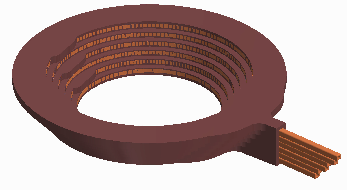
\includegraphics[]{\imagepath/single_coil_drawing/single_coil_drawing.pdf}
        \caption{Three-dimensional drawing of a Feshbach coil}
        \label{fig:single_coil_drawing}
    \end{subfigure}
    \hspace{0.03\textwidth}
    \begin{subfigure}[t]{0.48\textwidth}
        \centering
        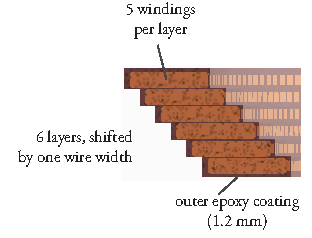
\includegraphics[]{\imagepath/coil_geometry_specification/coil_geometry_specification.pdf}
        \caption{Cross-section: The six winding layers are arranged in a parallelogram shape, with each layer having 5 windings.}
        \label{fig:coil_geometry_specification}
    \end{subfigure}
    \caption{Specified geometry and cross-section of the Feshbach coils}
\end{figure}

More details of the geometrical specification as well as some measured geometrical properties of the three coils are listed in the appendix chapter~\ref{ch:feshbach_coil_geometrical_properties}.

The coils will be held in place using holders designed by the engineering advisors of the FermiQP demonstrator, made out of the non-magnetic material PEEK. Massive spacers between the two coils tightly fix them for impeding vibrations and ensuring that they cannot change their distance due to any field gradient-induced forces.

\subsection*{Operational Properties}
The operational properties introduced in section \ref{ch:simulation} were simulated using the \textit{coil simulation library} and are listed in table~\ref{tab:operational_properties}.

In a four-point measurement, the resistance of the middle pancake of the \textit{Gauss} coil (wire length roughly $\frac{\SI{15.7}{\meter}}{3}$) with estimated \SI{6}{\meter} of supply line wire was measured to be \SI{12.8}{\milli\ohm}. The expected value of $\rho_\text{copper} \cdot \frac{(\SI{5}{\milli\meter})^2 - \pi(\SI{1.5}{\milli\meter})^2}{\SI{15.7}{\meter}/3 + \SI{6}{\meter}} \approx \SI{11}{\milli\ohm}$ is on the same order of magnitude. The experimenters reckon that the resistance might be higher than expected due the bends in the wire.

Additionally, the coil was set up to form an $LC$ circuit together with an oscilloscope of $C = \SI{15}{\pico\farad}$ to verify the simulated inductance of \SI{15}{\milli\henry}. In this setup, the supply lines of the coil were wound up to coils of $9$ windings with a radius of about \SI{11}{\centi\meter}, leading to an estimated additional inductance of $L_\text{supply} = \frac{N\Phi}{I} = \frac{N^2\mu_0\pi r}{2} \approx \SI{0.02}{\milli\henry}$. The resonance frequency of the circuit was experimentally determined as $f = \SI{3.19}{\mega\hertz}$ which allows to estimate the inductance of the coil:
\begin{align}
    f = \frac{1}{2\pi \sqrt{(L_\text{coil} + L_\text{supply})C}} ~\Rightarrow~ L_\text{coil} = \left(\frac{1}{2\pi f \sqrt{C}}\right)^2 - L_\text{supply} \approx \SI{0.15}{\milli\henry}
\end{align}
which corroborates that the simulated value is realistic.

\begin{table}
    \centering
    \begin{tabular}{rcc}
        \toprule
        \textbf{quantity} & \textbf{simulated value}  & \textbf{equation reference} \\
        \toprule
        wire length & \SI{15.7}{\meter} & \\
        resistance $R_\mathcal{C}$ & \SI{14.9}{\milli\ohm} & \eqref {eq:resistance_simulation} \\
        inductance $L_\mathcal{C}$ & \SI{0.15}{\milli\henry} & \eqref{eq:inductance_simulation} \\ 
        time constant $\tau_\mathcal{C}$ & \SI{9.9}{\milli\second} & \eqref{eq:time_constant_simulation}\\
        magnetic dipole moment $m_\mathcal{C}$ & \SI{265}{\ampere\square\meter} & \eqref{eq:dipole_moment_simulation} \\
        \bottomrule
    \end{tabular}
    \caption{Operational properties of the Feshbach coils determined using the \text{coil simulation library}}
    \label{tab:operational_properties}
\end{table}

\subsection*{Magnetic Fields}
Using a Sensys FGM3D/1000 fluxgate magnetic field probe (dominant relative error of \SI{0.5}{\percent}), the on-axis magnetic field produced by the three coils \textit{Gauss}, \textit{Maxwell}, and \textit{Tesla} at $I = \SI{1.000}{\ampere}$ was mapped, as displayed in figure~\ref{fig:single_coil_fields}. The measured values $B$ were fit to the following model for the on-axis field of \SI{30}{} spatially separated wire loops~\cite{demtroder_statische_2013}:
\begin{align}\label{eq:on_axis_field_model}
    \hat B[I, r, y_0](y) = \sum\limits_{a = 0}^5 \sum\limits_{c = 0}^4 \frac{\mu_0 I}{2} \frac{r_{ac}^2}{\left(r_{ac}^2 + (y - y_{ac})^2\right)^\frac{3}{2}}
\end{align}
with the position $y_{ac} = y_0 + (a - 2.5) w$ and the radius $r_{ac} = r + (c-2)w$ of a winding with on-axis index $a$, cross-axis index $c$, and a winding spacing $w$.

With root mean square error\footnote{$RMSE[B, \hat B] = \sqrt{\frac{1}{N}\sum_{i = 1}^N (B_i-\hat B_i)^2}$} values of $<\SI{3}{\milli\gauss}$, which is about \SI{e-3}{} of the maximum field, the model fits the observed field landscapes very well. From the resulting parameters $\hat I$, $\hat r$, and $\hat y_0$ (listed in table~\ref{tab:single_coil_fields_fit_parameters}) it can be concluded that the coils cannot produce the same maximum field and that they act like they are operated at different currents and/or have slightly different dimensions.\footnote{In the fit, the estimated parameters $\hat I$ and $\hat r$ are nearly collinear (correlation of \SI{99.9976}{\percent}), which can be understood from $\hat B \propto \frac{I}{r}$ for $y^2 \ll r^2$. This means that the deviations from the estimated field values cannot distinctively be attributed to either the radius or the current.}
Comparing the measured and the simulated fields via $RMSE[B, B_\text{simulated}]$ (see table~\ref{tab:single_coil_fields_fit_parameters}), one can also see that \textit{Tesla} matches the expected field landscape best, followed by \textit{Gauss}, and then \textit{Maxwell} very far off.

\begin{figure}
    \centering
    \begin{pgfpicture}
        \pgftext{%% Creator: Matplotlib, PGF backend
%%
%% To include the figure in your LaTeX document, write
%%   \input{<filename>.pgf}
%%
%% Make sure the required packages are loaded in your preamble
%%   \usepackage{pgf}
%%
%% Also ensure that all the required font packages are loaded; for instance,
%% the lmodern package is sometimes necessary when using math font.
%%   \usepackage{lmodern}
%%
%% Figures using additional raster images can only be included by \input if
%% they are in the same directory as the main LaTeX file. For loading figures
%% from other directories you can use the `import` package
%%   \usepackage{import}
%%
%% and then include the figures with
%%   \import{<path to file>}{<filename>.pgf}
%%
%% Matplotlib used the following preamble
%%   \usepackage{fontspec}
%%   \setmainfont{DejaVuSerif.ttf}[Path=\detokenize{/home/max/.conda/envs/3d_mot/lib/python3.9/site-packages/matplotlib/mpl-data/fonts/ttf/}]
%%   \setsansfont{DejaVuSans.ttf}[Path=\detokenize{/home/max/.conda/envs/3d_mot/lib/python3.9/site-packages/matplotlib/mpl-data/fonts/ttf/}]
%%   \setmonofont{DejaVuSansMono.ttf}[Path=\detokenize{/home/max/.conda/envs/3d_mot/lib/python3.9/site-packages/matplotlib/mpl-data/fonts/ttf/}]
%%
\begingroup%
\makeatletter%
\begin{pgfpicture}%
\pgfpathrectangle{\pgfpointorigin}{\pgfqpoint{5.830290in}{2.677849in}}%
\pgfusepath{use as bounding box, clip}%
\begin{pgfscope}%
\pgfsetbuttcap%
\pgfsetmiterjoin%
\pgfsetlinewidth{0.000000pt}%
\definecolor{currentstroke}{rgb}{1.000000,1.000000,1.000000}%
\pgfsetstrokecolor{currentstroke}%
\pgfsetstrokeopacity{0.000000}%
\pgfsetdash{}{0pt}%
\pgfpathmoveto{\pgfqpoint{0.000000in}{0.000000in}}%
\pgfpathlineto{\pgfqpoint{5.830290in}{0.000000in}}%
\pgfpathlineto{\pgfqpoint{5.830290in}{2.677849in}}%
\pgfpathlineto{\pgfqpoint{0.000000in}{2.677849in}}%
\pgfpathlineto{\pgfqpoint{0.000000in}{0.000000in}}%
\pgfpathclose%
\pgfusepath{}%
\end{pgfscope}%
\begin{pgfscope}%
\pgfsetbuttcap%
\pgfsetmiterjoin%
\definecolor{currentfill}{rgb}{1.000000,1.000000,1.000000}%
\pgfsetfillcolor{currentfill}%
\pgfsetlinewidth{0.000000pt}%
\definecolor{currentstroke}{rgb}{0.000000,0.000000,0.000000}%
\pgfsetstrokecolor{currentstroke}%
\pgfsetstrokeopacity{0.000000}%
\pgfsetdash{}{0pt}%
\pgfpathmoveto{\pgfqpoint{0.652070in}{0.494721in}}%
\pgfpathlineto{\pgfqpoint{5.730290in}{0.494721in}}%
\pgfpathlineto{\pgfqpoint{5.730290in}{2.577849in}}%
\pgfpathlineto{\pgfqpoint{0.652070in}{2.577849in}}%
\pgfpathlineto{\pgfqpoint{0.652070in}{0.494721in}}%
\pgfpathclose%
\pgfusepath{fill}%
\end{pgfscope}%
\begin{pgfscope}%
\pgfpathrectangle{\pgfqpoint{0.652070in}{0.494721in}}{\pgfqpoint{5.078220in}{2.083128in}}%
\pgfusepath{clip}%
\pgfsetbuttcap%
\pgfsetroundjoin%
\definecolor{currentfill}{rgb}{0.313725,0.741176,0.913725}%
\pgfsetfillcolor{currentfill}%
\pgfsetlinewidth{1.505625pt}%
\definecolor{currentstroke}{rgb}{0.313725,0.741176,0.913725}%
\pgfsetstrokecolor{currentstroke}%
\pgfsetdash{}{0pt}%
\pgfsys@defobject{currentmarker}{\pgfqpoint{-0.021960in}{-0.021960in}}{\pgfqpoint{0.021960in}{0.021960in}}{%
\pgfpathmoveto{\pgfqpoint{-0.021960in}{-0.021960in}}%
\pgfpathlineto{\pgfqpoint{0.021960in}{0.021960in}}%
\pgfpathmoveto{\pgfqpoint{-0.021960in}{0.021960in}}%
\pgfpathlineto{\pgfqpoint{0.021960in}{-0.021960in}}%
\pgfusepath{stroke,fill}%
}%
\begin{pgfscope}%
\pgfsys@transformshift{1.190787in}{2.212826in}%
\pgfsys@useobject{currentmarker}{}%
\end{pgfscope}%
\begin{pgfscope}%
\pgfsys@transformshift{1.230561in}{2.233834in}%
\pgfsys@useobject{currentmarker}{}%
\end{pgfscope}%
\begin{pgfscope}%
\pgfsys@transformshift{1.260391in}{2.247102in}%
\pgfsys@useobject{currentmarker}{}%
\end{pgfscope}%
\begin{pgfscope}%
\pgfsys@transformshift{1.296613in}{2.265898in}%
\pgfsys@useobject{currentmarker}{}%
\end{pgfscope}%
\begin{pgfscope}%
\pgfsys@transformshift{1.332125in}{2.284694in}%
\pgfsys@useobject{currentmarker}{}%
\end{pgfscope}%
\begin{pgfscope}%
\pgfsys@transformshift{1.367282in}{2.296856in}%
\pgfsys@useobject{currentmarker}{}%
\end{pgfscope}%
\begin{pgfscope}%
\pgfsys@transformshift{1.402439in}{2.310124in}%
\pgfsys@useobject{currentmarker}{}%
\end{pgfscope}%
\begin{pgfscope}%
\pgfsys@transformshift{1.440082in}{2.325603in}%
\pgfsys@useobject{currentmarker}{}%
\end{pgfscope}%
\begin{pgfscope}%
\pgfsys@transformshift{1.472753in}{2.337765in}%
\pgfsys@useobject{currentmarker}{}%
\end{pgfscope}%
\begin{pgfscope}%
\pgfsys@transformshift{1.511106in}{2.352139in}%
\pgfsys@useobject{currentmarker}{}%
\end{pgfscope}%
\begin{pgfscope}%
\pgfsys@transformshift{1.544487in}{2.362090in}%
\pgfsys@useobject{currentmarker}{}%
\end{pgfscope}%
\begin{pgfscope}%
\pgfsys@transformshift{1.581064in}{2.372041in}%
\pgfsys@useobject{currentmarker}{}%
\end{pgfscope}%
\begin{pgfscope}%
\pgfsys@transformshift{1.619417in}{2.383097in}%
\pgfsys@useobject{currentmarker}{}%
\end{pgfscope}%
\begin{pgfscope}%
\pgfsys@transformshift{1.653864in}{2.391942in}%
\pgfsys@useobject{currentmarker}{}%
\end{pgfscope}%
\begin{pgfscope}%
\pgfsys@transformshift{1.686535in}{2.398576in}%
\pgfsys@useobject{currentmarker}{}%
\end{pgfscope}%
\begin{pgfscope}%
\pgfsys@transformshift{1.721692in}{2.406316in}%
\pgfsys@useobject{currentmarker}{}%
\end{pgfscope}%
\begin{pgfscope}%
\pgfsys@transformshift{1.756849in}{2.411844in}%
\pgfsys@useobject{currentmarker}{}%
\end{pgfscope}%
\begin{pgfscope}%
\pgfsys@transformshift{1.793426in}{2.417373in}%
\pgfsys@useobject{currentmarker}{}%
\end{pgfscope}%
\begin{pgfscope}%
\pgfsys@transformshift{1.831424in}{2.420689in}%
\pgfsys@useobject{currentmarker}{}%
\end{pgfscope}%
\begin{pgfscope}%
\pgfsys@transformshift{1.865160in}{2.425112in}%
\pgfsys@useobject{currentmarker}{}%
\end{pgfscope}%
\begin{pgfscope}%
\pgfsys@transformshift{1.901383in}{2.426218in}%
\pgfsys@useobject{currentmarker}{}%
\end{pgfscope}%
\begin{pgfscope}%
\pgfsys@transformshift{1.935119in}{2.426218in}%
\pgfsys@useobject{currentmarker}{}%
\end{pgfscope}%
\begin{pgfscope}%
\pgfsys@transformshift{1.971341in}{2.426218in}%
\pgfsys@useobject{currentmarker}{}%
\end{pgfscope}%
\begin{pgfscope}%
\pgfsys@transformshift{2.006853in}{2.426218in}%
\pgfsys@useobject{currentmarker}{}%
\end{pgfscope}%
\begin{pgfscope}%
\pgfsys@transformshift{2.043431in}{2.422901in}%
\pgfsys@useobject{currentmarker}{}%
\end{pgfscope}%
\begin{pgfscope}%
\pgfsys@transformshift{2.080363in}{2.419584in}%
\pgfsys@useobject{currentmarker}{}%
\end{pgfscope}%
\begin{pgfscope}%
\pgfsys@transformshift{2.112679in}{2.416267in}%
\pgfsys@useobject{currentmarker}{}%
\end{pgfscope}%
\begin{pgfscope}%
\pgfsys@transformshift{2.148902in}{2.410739in}%
\pgfsys@useobject{currentmarker}{}%
\end{pgfscope}%
\begin{pgfscope}%
\pgfsys@transformshift{2.183348in}{2.402999in}%
\pgfsys@useobject{currentmarker}{}%
\end{pgfscope}%
\begin{pgfscope}%
\pgfsys@transformshift{2.220281in}{2.397471in}%
\pgfsys@useobject{currentmarker}{}%
\end{pgfscope}%
\begin{pgfscope}%
\pgfsys@transformshift{2.256858in}{2.388625in}%
\pgfsys@useobject{currentmarker}{}%
\end{pgfscope}%
\begin{pgfscope}%
\pgfsys@transformshift{2.293436in}{2.377569in}%
\pgfsys@useobject{currentmarker}{}%
\end{pgfscope}%
\begin{pgfscope}%
\pgfsys@transformshift{2.327172in}{2.367618in}%
\pgfsys@useobject{currentmarker}{}%
\end{pgfscope}%
\begin{pgfscope}%
\pgfsys@transformshift{2.361264in}{2.357667in}%
\pgfsys@useobject{currentmarker}{}%
\end{pgfscope}%
\begin{pgfscope}%
\pgfsys@transformshift{2.399972in}{2.344399in}%
\pgfsys@useobject{currentmarker}{}%
\end{pgfscope}%
\begin{pgfscope}%
\pgfsys@transformshift{2.436549in}{2.331131in}%
\pgfsys@useobject{currentmarker}{}%
\end{pgfscope}%
\begin{pgfscope}%
\pgfsys@transformshift{2.467800in}{2.318969in}%
\pgfsys@useobject{currentmarker}{}%
\end{pgfscope}%
\begin{pgfscope}%
\pgfsys@transformshift{2.505087in}{2.302384in}%
\pgfsys@useobject{currentmarker}{}%
\end{pgfscope}%
\begin{pgfscope}%
\pgfsys@transformshift{2.539179in}{2.286905in}%
\pgfsys@useobject{currentmarker}{}%
\end{pgfscope}%
\begin{pgfscope}%
\pgfsys@transformshift{2.577177in}{2.270320in}%
\pgfsys@useobject{currentmarker}{}%
\end{pgfscope}%
\begin{pgfscope}%
\pgfsys@transformshift{2.610203in}{2.252630in}%
\pgfsys@useobject{currentmarker}{}%
\end{pgfscope}%
\begin{pgfscope}%
\pgfsys@transformshift{2.645715in}{2.234939in}%
\pgfsys@useobject{currentmarker}{}%
\end{pgfscope}%
\begin{pgfscope}%
\pgfsys@transformshift{2.683713in}{2.215038in}%
\pgfsys@useobject{currentmarker}{}%
\end{pgfscope}%
\begin{pgfscope}%
\pgfsys@transformshift{2.720645in}{2.194030in}%
\pgfsys@useobject{currentmarker}{}%
\end{pgfscope}%
\begin{pgfscope}%
\pgfsys@transformshift{2.751896in}{2.177445in}%
\pgfsys@useobject{currentmarker}{}%
\end{pgfscope}%
\begin{pgfscope}%
\pgfsys@transformshift{2.787053in}{2.155332in}%
\pgfsys@useobject{currentmarker}{}%
\end{pgfscope}%
\begin{pgfscope}%
\pgfsys@transformshift{2.822565in}{2.134325in}%
\pgfsys@useobject{currentmarker}{}%
\end{pgfscope}%
\begin{pgfscope}%
\pgfsys@transformshift{2.857722in}{2.111106in}%
\pgfsys@useobject{currentmarker}{}%
\end{pgfscope}%
\begin{pgfscope}%
\pgfsys@transformshift{2.896075in}{2.087887in}%
\pgfsys@useobject{currentmarker}{}%
\end{pgfscope}%
\begin{pgfscope}%
\pgfsys@transformshift{2.933007in}{2.066880in}%
\pgfsys@useobject{currentmarker}{}%
\end{pgfscope}%
\begin{pgfscope}%
\pgfsys@transformshift{2.964968in}{2.044767in}%
\pgfsys@useobject{currentmarker}{}%
\end{pgfscope}%
\begin{pgfscope}%
\pgfsys@transformshift{3.001190in}{2.020442in}%
\pgfsys@useobject{currentmarker}{}%
\end{pgfscope}%
\begin{pgfscope}%
\pgfsys@transformshift{3.035282in}{1.999435in}%
\pgfsys@useobject{currentmarker}{}%
\end{pgfscope}%
\begin{pgfscope}%
\pgfsys@transformshift{3.071149in}{1.974005in}%
\pgfsys@useobject{currentmarker}{}%
\end{pgfscope}%
\begin{pgfscope}%
\pgfsys@transformshift{3.105951in}{1.949680in}%
\pgfsys@useobject{currentmarker}{}%
\end{pgfscope}%
\begin{pgfscope}%
\pgfsys@transformshift{3.141463in}{1.926462in}%
\pgfsys@useobject{currentmarker}{}%
\end{pgfscope}%
\begin{pgfscope}%
\pgfsys@transformshift{3.181591in}{1.895503in}%
\pgfsys@useobject{currentmarker}{}%
\end{pgfscope}%
\begin{pgfscope}%
\pgfsys@transformshift{3.214973in}{1.871179in}%
\pgfsys@useobject{currentmarker}{}%
\end{pgfscope}%
\begin{pgfscope}%
\pgfsys@transformshift{3.254391in}{1.844643in}%
\pgfsys@useobject{currentmarker}{}%
\end{pgfscope}%
\begin{pgfscope}%
\pgfsys@transformshift{3.285287in}{1.819213in}%
\pgfsys@useobject{currentmarker}{}%
\end{pgfscope}%
\begin{pgfscope}%
\pgfsys@transformshift{3.320443in}{1.797100in}%
\pgfsys@useobject{currentmarker}{}%
\end{pgfscope}%
\begin{pgfscope}%
\pgfsys@transformshift{3.354535in}{1.771670in}%
\pgfsys@useobject{currentmarker}{}%
\end{pgfscope}%
\begin{pgfscope}%
\pgfsys@transformshift{3.392888in}{1.744029in}%
\pgfsys@useobject{currentmarker}{}%
\end{pgfscope}%
\begin{pgfscope}%
\pgfsys@transformshift{3.428045in}{1.717493in}%
\pgfsys@useobject{currentmarker}{}%
\end{pgfscope}%
\begin{pgfscope}%
\pgfsys@transformshift{3.463912in}{1.688746in}%
\pgfsys@useobject{currentmarker}{}%
\end{pgfscope}%
\begin{pgfscope}%
\pgfsys@transformshift{3.498714in}{1.664421in}%
\pgfsys@useobject{currentmarker}{}%
\end{pgfscope}%
\begin{pgfscope}%
\pgfsys@transformshift{3.536001in}{1.638991in}%
\pgfsys@useobject{currentmarker}{}%
\end{pgfscope}%
\begin{pgfscope}%
\pgfsys@transformshift{3.571869in}{1.611350in}%
\pgfsys@useobject{currentmarker}{}%
\end{pgfscope}%
\begin{pgfscope}%
\pgfsys@transformshift{3.605960in}{1.587026in}%
\pgfsys@useobject{currentmarker}{}%
\end{pgfscope}%
\begin{pgfscope}%
\pgfsys@transformshift{3.643248in}{1.561595in}%
\pgfsys@useobject{currentmarker}{}%
\end{pgfscope}%
\begin{pgfscope}%
\pgfsys@transformshift{3.680535in}{1.532848in}%
\pgfsys@useobject{currentmarker}{}%
\end{pgfscope}%
\begin{pgfscope}%
\pgfsys@transformshift{3.711786in}{1.511841in}%
\pgfsys@useobject{currentmarker}{}%
\end{pgfscope}%
\begin{pgfscope}%
\pgfsys@transformshift{3.747653in}{1.484200in}%
\pgfsys@useobject{currentmarker}{}%
\end{pgfscope}%
\begin{pgfscope}%
\pgfsys@transformshift{3.784586in}{1.460981in}%
\pgfsys@useobject{currentmarker}{}%
\end{pgfscope}%
\begin{pgfscope}%
\pgfsys@transformshift{3.820808in}{1.433339in}%
\pgfsys@useobject{currentmarker}{}%
\end{pgfscope}%
\begin{pgfscope}%
\pgfsys@transformshift{3.855965in}{1.409015in}%
\pgfsys@useobject{currentmarker}{}%
\end{pgfscope}%
\begin{pgfscope}%
\pgfsys@transformshift{3.889701in}{1.385796in}%
\pgfsys@useobject{currentmarker}{}%
\end{pgfscope}%
\begin{pgfscope}%
\pgfsys@transformshift{3.928409in}{1.359261in}%
\pgfsys@useobject{currentmarker}{}%
\end{pgfscope}%
\begin{pgfscope}%
\pgfsys@transformshift{3.963921in}{1.334936in}%
\pgfsys@useobject{currentmarker}{}%
\end{pgfscope}%
\begin{pgfscope}%
\pgfsys@transformshift{4.001209in}{1.308400in}%
\pgfsys@useobject{currentmarker}{}%
\end{pgfscope}%
\begin{pgfscope}%
\pgfsys@transformshift{4.038497in}{1.286287in}%
\pgfsys@useobject{currentmarker}{}%
\end{pgfscope}%
\begin{pgfscope}%
\pgfsys@transformshift{4.070457in}{1.266386in}%
\pgfsys@useobject{currentmarker}{}%
\end{pgfscope}%
\begin{pgfscope}%
\pgfsys@transformshift{4.107035in}{1.242061in}%
\pgfsys@useobject{currentmarker}{}%
\end{pgfscope}%
\begin{pgfscope}%
\pgfsys@transformshift{4.138641in}{1.223265in}%
\pgfsys@useobject{currentmarker}{}%
\end{pgfscope}%
\begin{pgfscope}%
\pgfsys@transformshift{4.175573in}{1.198941in}%
\pgfsys@useobject{currentmarker}{}%
\end{pgfscope}%
\begin{pgfscope}%
\pgfsys@transformshift{4.210020in}{1.177933in}%
\pgfsys@useobject{currentmarker}{}%
\end{pgfscope}%
\begin{pgfscope}%
\pgfsys@transformshift{4.249438in}{1.154714in}%
\pgfsys@useobject{currentmarker}{}%
\end{pgfscope}%
\begin{pgfscope}%
\pgfsys@transformshift{4.283885in}{1.134813in}%
\pgfsys@useobject{currentmarker}{}%
\end{pgfscope}%
\begin{pgfscope}%
\pgfsys@transformshift{4.318331in}{1.114911in}%
\pgfsys@useobject{currentmarker}{}%
\end{pgfscope}%
\begin{pgfscope}%
\pgfsys@transformshift{4.351003in}{1.092798in}%
\pgfsys@useobject{currentmarker}{}%
\end{pgfscope}%
\begin{pgfscope}%
\pgfsys@transformshift{4.390066in}{1.071790in}%
\pgfsys@useobject{currentmarker}{}%
\end{pgfscope}%
\begin{pgfscope}%
\pgfsys@transformshift{4.419186in}{1.051888in}%
\pgfsys@useobject{currentmarker}{}%
\end{pgfscope}%
\begin{pgfscope}%
\pgfsys@transformshift{4.461445in}{1.033092in}%
\pgfsys@useobject{currentmarker}{}%
\end{pgfscope}%
\begin{pgfscope}%
\pgfsys@transformshift{4.496957in}{1.014296in}%
\pgfsys@useobject{currentmarker}{}%
\end{pgfscope}%
\begin{pgfscope}%
\pgfsys@transformshift{4.529983in}{0.997711in}%
\pgfsys@useobject{currentmarker}{}%
\end{pgfscope}%
\begin{pgfscope}%
\pgfsys@transformshift{4.565495in}{0.978915in}%
\pgfsys@useobject{currentmarker}{}%
\end{pgfscope}%
\begin{pgfscope}%
\pgfsys@transformshift{4.599942in}{0.961225in}%
\pgfsys@useobject{currentmarker}{}%
\end{pgfscope}%
\begin{pgfscope}%
\pgfsys@transformshift{4.639360in}{0.940217in}%
\pgfsys@useobject{currentmarker}{}%
\end{pgfscope}%
\begin{pgfscope}%
\pgfsys@transformshift{4.674872in}{0.922527in}%
\pgfsys@useobject{currentmarker}{}%
\end{pgfscope}%
\begin{pgfscope}%
\pgfsys@transformshift{4.711450in}{0.902625in}%
\pgfsys@useobject{currentmarker}{}%
\end{pgfscope}%
\begin{pgfscope}%
\pgfsys@transformshift{4.741280in}{0.889357in}%
\pgfsys@useobject{currentmarker}{}%
\end{pgfscope}%
\begin{pgfscope}%
\pgfsys@transformshift{4.782829in}{0.869455in}%
\pgfsys@useobject{currentmarker}{}%
\end{pgfscope}%
\begin{pgfscope}%
\pgfsys@transformshift{4.811949in}{0.856187in}%
\pgfsys@useobject{currentmarker}{}%
\end{pgfscope}%
\begin{pgfscope}%
\pgfsys@transformshift{4.851367in}{0.838497in}%
\pgfsys@useobject{currentmarker}{}%
\end{pgfscope}%
\begin{pgfscope}%
\pgfsys@transformshift{4.890075in}{0.820807in}%
\pgfsys@useobject{currentmarker}{}%
\end{pgfscope}%
\begin{pgfscope}%
\pgfsys@transformshift{4.918840in}{0.811961in}%
\pgfsys@useobject{currentmarker}{}%
\end{pgfscope}%
\begin{pgfscope}%
\pgfsys@transformshift{4.956127in}{0.793165in}%
\pgfsys@useobject{currentmarker}{}%
\end{pgfscope}%
\begin{pgfscope}%
\pgfsys@transformshift{4.993060in}{0.776580in}%
\pgfsys@useobject{currentmarker}{}%
\end{pgfscope}%
\begin{pgfscope}%
\pgfsys@transformshift{5.026441in}{0.763312in}%
\pgfsys@useobject{currentmarker}{}%
\end{pgfscope}%
\begin{pgfscope}%
\pgfsys@transformshift{5.063019in}{0.748939in}%
\pgfsys@useobject{currentmarker}{}%
\end{pgfscope}%
\end{pgfscope}%
\begin{pgfscope}%
\pgfpathrectangle{\pgfqpoint{0.652070in}{0.494721in}}{\pgfqpoint{5.078220in}{2.083128in}}%
\pgfusepath{clip}%
\pgfsetbuttcap%
\pgfsetroundjoin%
\definecolor{currentfill}{rgb}{0.603922,0.356863,0.568627}%
\pgfsetfillcolor{currentfill}%
\pgfsetlinewidth{1.505625pt}%
\definecolor{currentstroke}{rgb}{0.603922,0.356863,0.568627}%
\pgfsetstrokecolor{currentstroke}%
\pgfsetdash{}{0pt}%
\pgfsys@defobject{currentmarker}{\pgfqpoint{-0.021960in}{-0.021960in}}{\pgfqpoint{0.021960in}{0.021960in}}{%
\pgfpathmoveto{\pgfqpoint{-0.021960in}{-0.021960in}}%
\pgfpathlineto{\pgfqpoint{0.021960in}{0.021960in}}%
\pgfpathmoveto{\pgfqpoint{-0.021960in}{0.021960in}}%
\pgfpathlineto{\pgfqpoint{0.021960in}{-0.021960in}}%
\pgfusepath{stroke,fill}%
}%
\begin{pgfscope}%
\pgfsys@transformshift{1.168414in}{2.090099in}%
\pgfsys@useobject{currentmarker}{}%
\end{pgfscope}%
\begin{pgfscope}%
\pgfsys@transformshift{1.204992in}{2.108895in}%
\pgfsys@useobject{currentmarker}{}%
\end{pgfscope}%
\begin{pgfscope}%
\pgfsys@transformshift{1.240504in}{2.125480in}%
\pgfsys@useobject{currentmarker}{}%
\end{pgfscope}%
\begin{pgfscope}%
\pgfsys@transformshift{1.276016in}{2.139853in}%
\pgfsys@useobject{currentmarker}{}%
\end{pgfscope}%
\begin{pgfscope}%
\pgfsys@transformshift{1.309397in}{2.155332in}%
\pgfsys@useobject{currentmarker}{}%
\end{pgfscope}%
\begin{pgfscope}%
\pgfsys@transformshift{1.344909in}{2.169706in}%
\pgfsys@useobject{currentmarker}{}%
\end{pgfscope}%
\begin{pgfscope}%
\pgfsys@transformshift{1.383262in}{2.186291in}%
\pgfsys@useobject{currentmarker}{}%
\end{pgfscope}%
\begin{pgfscope}%
\pgfsys@transformshift{1.416999in}{2.197347in}%
\pgfsys@useobject{currentmarker}{}%
\end{pgfscope}%
\begin{pgfscope}%
\pgfsys@transformshift{1.453931in}{2.210615in}%
\pgfsys@useobject{currentmarker}{}%
\end{pgfscope}%
\begin{pgfscope}%
\pgfsys@transformshift{1.490509in}{2.222777in}%
\pgfsys@useobject{currentmarker}{}%
\end{pgfscope}%
\begin{pgfscope}%
\pgfsys@transformshift{1.522825in}{2.232728in}%
\pgfsys@useobject{currentmarker}{}%
\end{pgfscope}%
\begin{pgfscope}%
\pgfsys@transformshift{1.559757in}{2.243785in}%
\pgfsys@useobject{currentmarker}{}%
\end{pgfscope}%
\begin{pgfscope}%
\pgfsys@transformshift{1.596334in}{2.251524in}%
\pgfsys@useobject{currentmarker}{}%
\end{pgfscope}%
\begin{pgfscope}%
\pgfsys@transformshift{1.630781in}{2.260369in}%
\pgfsys@useobject{currentmarker}{}%
\end{pgfscope}%
\begin{pgfscope}%
\pgfsys@transformshift{1.665583in}{2.268109in}%
\pgfsys@useobject{currentmarker}{}%
\end{pgfscope}%
\begin{pgfscope}%
\pgfsys@transformshift{1.700740in}{2.274743in}%
\pgfsys@useobject{currentmarker}{}%
\end{pgfscope}%
\begin{pgfscope}%
\pgfsys@transformshift{1.742289in}{2.281377in}%
\pgfsys@useobject{currentmarker}{}%
\end{pgfscope}%
\begin{pgfscope}%
\pgfsys@transformshift{1.771409in}{2.285800in}%
\pgfsys@useobject{currentmarker}{}%
\end{pgfscope}%
\begin{pgfscope}%
\pgfsys@transformshift{1.806921in}{2.286905in}%
\pgfsys@useobject{currentmarker}{}%
\end{pgfscope}%
\begin{pgfscope}%
\pgfsys@transformshift{1.843498in}{2.292433in}%
\pgfsys@useobject{currentmarker}{}%
\end{pgfscope}%
\begin{pgfscope}%
\pgfsys@transformshift{1.877945in}{2.294645in}%
\pgfsys@useobject{currentmarker}{}%
\end{pgfscope}%
\begin{pgfscope}%
\pgfsys@transformshift{1.913102in}{2.295750in}%
\pgfsys@useobject{currentmarker}{}%
\end{pgfscope}%
\begin{pgfscope}%
\pgfsys@transformshift{1.949324in}{2.295750in}%
\pgfsys@useobject{currentmarker}{}%
\end{pgfscope}%
\begin{pgfscope}%
\pgfsys@transformshift{1.985546in}{2.294645in}%
\pgfsys@useobject{currentmarker}{}%
\end{pgfscope}%
\begin{pgfscope}%
\pgfsys@transformshift{2.021058in}{2.292433in}%
\pgfsys@useobject{currentmarker}{}%
\end{pgfscope}%
\begin{pgfscope}%
\pgfsys@transformshift{2.057281in}{2.290222in}%
\pgfsys@useobject{currentmarker}{}%
\end{pgfscope}%
\begin{pgfscope}%
\pgfsys@transformshift{2.092793in}{2.286905in}%
\pgfsys@useobject{currentmarker}{}%
\end{pgfscope}%
\begin{pgfscope}%
\pgfsys@transformshift{2.127594in}{2.281377in}%
\pgfsys@useobject{currentmarker}{}%
\end{pgfscope}%
\begin{pgfscope}%
\pgfsys@transformshift{2.163817in}{2.275849in}%
\pgfsys@useobject{currentmarker}{}%
\end{pgfscope}%
\begin{pgfscope}%
\pgfsys@transformshift{2.199684in}{2.268109in}%
\pgfsys@useobject{currentmarker}{}%
\end{pgfscope}%
\begin{pgfscope}%
\pgfsys@transformshift{2.234841in}{2.261475in}%
\pgfsys@useobject{currentmarker}{}%
\end{pgfscope}%
\begin{pgfscope}%
\pgfsys@transformshift{2.270353in}{2.252630in}%
\pgfsys@useobject{currentmarker}{}%
\end{pgfscope}%
\begin{pgfscope}%
\pgfsys@transformshift{2.305155in}{2.244890in}%
\pgfsys@useobject{currentmarker}{}%
\end{pgfscope}%
\begin{pgfscope}%
\pgfsys@transformshift{2.339246in}{2.234939in}%
\pgfsys@useobject{currentmarker}{}%
\end{pgfscope}%
\begin{pgfscope}%
\pgfsys@transformshift{2.374403in}{2.222777in}%
\pgfsys@useobject{currentmarker}{}%
\end{pgfscope}%
\begin{pgfscope}%
\pgfsys@transformshift{2.411335in}{2.210615in}%
\pgfsys@useobject{currentmarker}{}%
\end{pgfscope}%
\begin{pgfscope}%
\pgfsys@transformshift{2.446848in}{2.197347in}%
\pgfsys@useobject{currentmarker}{}%
\end{pgfscope}%
\begin{pgfscope}%
\pgfsys@transformshift{2.484845in}{2.182974in}%
\pgfsys@useobject{currentmarker}{}%
\end{pgfscope}%
\begin{pgfscope}%
\pgfsys@transformshift{2.518582in}{2.168600in}%
\pgfsys@useobject{currentmarker}{}%
\end{pgfscope}%
\begin{pgfscope}%
\pgfsys@transformshift{2.558710in}{2.152015in}%
\pgfsys@useobject{currentmarker}{}%
\end{pgfscope}%
\begin{pgfscope}%
\pgfsys@transformshift{2.590671in}{2.137642in}%
\pgfsys@useobject{currentmarker}{}%
\end{pgfscope}%
\begin{pgfscope}%
\pgfsys@transformshift{2.625473in}{2.121057in}%
\pgfsys@useobject{currentmarker}{}%
\end{pgfscope}%
\begin{pgfscope}%
\pgfsys@transformshift{2.659209in}{2.104472in}%
\pgfsys@useobject{currentmarker}{}%
\end{pgfscope}%
\begin{pgfscope}%
\pgfsys@transformshift{2.695077in}{2.083465in}%
\pgfsys@useobject{currentmarker}{}%
\end{pgfscope}%
\begin{pgfscope}%
\pgfsys@transformshift{2.735560in}{2.065774in}%
\pgfsys@useobject{currentmarker}{}%
\end{pgfscope}%
\begin{pgfscope}%
\pgfsys@transformshift{2.768587in}{2.048084in}%
\pgfsys@useobject{currentmarker}{}%
\end{pgfscope}%
\begin{pgfscope}%
\pgfsys@transformshift{2.801968in}{2.028182in}%
\pgfsys@useobject{currentmarker}{}%
\end{pgfscope}%
\begin{pgfscope}%
\pgfsys@transformshift{2.839255in}{2.008280in}%
\pgfsys@useobject{currentmarker}{}%
\end{pgfscope}%
\begin{pgfscope}%
\pgfsys@transformshift{2.871571in}{1.988378in}%
\pgfsys@useobject{currentmarker}{}%
\end{pgfscope}%
\begin{pgfscope}%
\pgfsys@transformshift{2.909214in}{1.966265in}%
\pgfsys@useobject{currentmarker}{}%
\end{pgfscope}%
\begin{pgfscope}%
\pgfsys@transformshift{2.947567in}{1.943046in}%
\pgfsys@useobject{currentmarker}{}%
\end{pgfscope}%
\begin{pgfscope}%
\pgfsys@transformshift{2.982014in}{1.920933in}%
\pgfsys@useobject{currentmarker}{}%
\end{pgfscope}%
\begin{pgfscope}%
\pgfsys@transformshift{3.017881in}{1.897715in}%
\pgfsys@useobject{currentmarker}{}%
\end{pgfscope}%
\begin{pgfscope}%
\pgfsys@transformshift{3.049487in}{1.877813in}%
\pgfsys@useobject{currentmarker}{}%
\end{pgfscope}%
\begin{pgfscope}%
\pgfsys@transformshift{3.086419in}{1.855700in}%
\pgfsys@useobject{currentmarker}{}%
\end{pgfscope}%
\begin{pgfscope}%
\pgfsys@transformshift{3.122286in}{1.831375in}%
\pgfsys@useobject{currentmarker}{}%
\end{pgfscope}%
\begin{pgfscope}%
\pgfsys@transformshift{3.162415in}{1.803734in}%
\pgfsys@useobject{currentmarker}{}%
\end{pgfscope}%
\begin{pgfscope}%
\pgfsys@transformshift{3.191535in}{1.784938in}%
\pgfsys@useobject{currentmarker}{}%
\end{pgfscope}%
\begin{pgfscope}%
\pgfsys@transformshift{3.226692in}{1.762825in}%
\pgfsys@useobject{currentmarker}{}%
\end{pgfscope}%
\begin{pgfscope}%
\pgfsys@transformshift{3.265045in}{1.735183in}%
\pgfsys@useobject{currentmarker}{}%
\end{pgfscope}%
\begin{pgfscope}%
\pgfsys@transformshift{3.302687in}{1.708648in}%
\pgfsys@useobject{currentmarker}{}%
\end{pgfscope}%
\begin{pgfscope}%
\pgfsys@transformshift{3.334293in}{1.687640in}%
\pgfsys@useobject{currentmarker}{}%
\end{pgfscope}%
\begin{pgfscope}%
\pgfsys@transformshift{3.372291in}{1.659999in}%
\pgfsys@useobject{currentmarker}{}%
\end{pgfscope}%
\begin{pgfscope}%
\pgfsys@transformshift{3.409579in}{1.636780in}%
\pgfsys@useobject{currentmarker}{}%
\end{pgfscope}%
\begin{pgfscope}%
\pgfsys@transformshift{3.445091in}{1.611350in}%
\pgfsys@useobject{currentmarker}{}%
\end{pgfscope}%
\begin{pgfscope}%
\pgfsys@transformshift{3.483444in}{1.587026in}%
\pgfsys@useobject{currentmarker}{}%
\end{pgfscope}%
\begin{pgfscope}%
\pgfsys@transformshift{3.518601in}{1.561595in}%
\pgfsys@useobject{currentmarker}{}%
\end{pgfscope}%
\begin{pgfscope}%
\pgfsys@transformshift{3.552337in}{1.539482in}%
\pgfsys@useobject{currentmarker}{}%
\end{pgfscope}%
\begin{pgfscope}%
\pgfsys@transformshift{3.588914in}{1.515158in}%
\pgfsys@useobject{currentmarker}{}%
\end{pgfscope}%
\begin{pgfscope}%
\pgfsys@transformshift{3.630819in}{1.485305in}%
\pgfsys@useobject{currentmarker}{}%
\end{pgfscope}%
\begin{pgfscope}%
\pgfsys@transformshift{3.658873in}{1.462086in}%
\pgfsys@useobject{currentmarker}{}%
\end{pgfscope}%
\begin{pgfscope}%
\pgfsys@transformshift{3.693675in}{1.443290in}%
\pgfsys@useobject{currentmarker}{}%
\end{pgfscope}%
\begin{pgfscope}%
\pgfsys@transformshift{3.729187in}{1.420072in}%
\pgfsys@useobject{currentmarker}{}%
\end{pgfscope}%
\begin{pgfscope}%
\pgfsys@transformshift{3.771446in}{1.391325in}%
\pgfsys@useobject{currentmarker}{}%
\end{pgfscope}%
\begin{pgfscope}%
\pgfsys@transformshift{3.801987in}{1.371423in}%
\pgfsys@useobject{currentmarker}{}%
\end{pgfscope}%
\begin{pgfscope}%
\pgfsys@transformshift{3.838209in}{1.347098in}%
\pgfsys@useobject{currentmarker}{}%
\end{pgfscope}%
\begin{pgfscope}%
\pgfsys@transformshift{3.872655in}{1.323880in}%
\pgfsys@useobject{currentmarker}{}%
\end{pgfscope}%
\begin{pgfscope}%
\pgfsys@transformshift{3.912074in}{1.300661in}%
\pgfsys@useobject{currentmarker}{}%
\end{pgfscope}%
\begin{pgfscope}%
\pgfsys@transformshift{3.946521in}{1.278548in}%
\pgfsys@useobject{currentmarker}{}%
\end{pgfscope}%
\begin{pgfscope}%
\pgfsys@transformshift{3.983808in}{1.252012in}%
\pgfsys@useobject{currentmarker}{}%
\end{pgfscope}%
\begin{pgfscope}%
\pgfsys@transformshift{4.020386in}{1.233216in}%
\pgfsys@useobject{currentmarker}{}%
\end{pgfscope}%
\begin{pgfscope}%
\pgfsys@transformshift{4.054832in}{1.211103in}%
\pgfsys@useobject{currentmarker}{}%
\end{pgfscope}%
\begin{pgfscope}%
\pgfsys@transformshift{4.084662in}{1.194518in}%
\pgfsys@useobject{currentmarker}{}%
\end{pgfscope}%
\begin{pgfscope}%
\pgfsys@transformshift{4.121240in}{1.170194in}%
\pgfsys@useobject{currentmarker}{}%
\end{pgfscope}%
\begin{pgfscope}%
\pgfsys@transformshift{4.159593in}{1.149186in}%
\pgfsys@useobject{currentmarker}{}%
\end{pgfscope}%
\begin{pgfscope}%
\pgfsys@transformshift{4.197591in}{1.128179in}%
\pgfsys@useobject{currentmarker}{}%
\end{pgfscope}%
\begin{pgfscope}%
\pgfsys@transformshift{4.228131in}{1.110488in}%
\pgfsys@useobject{currentmarker}{}%
\end{pgfscope}%
\begin{pgfscope}%
\pgfsys@transformshift{4.265063in}{1.087269in}%
\pgfsys@useobject{currentmarker}{}%
\end{pgfscope}%
\begin{pgfscope}%
\pgfsys@transformshift{4.297379in}{1.071790in}%
\pgfsys@useobject{currentmarker}{}%
\end{pgfscope}%
\begin{pgfscope}%
\pgfsys@transformshift{4.334667in}{1.050783in}%
\pgfsys@useobject{currentmarker}{}%
\end{pgfscope}%
\begin{pgfscope}%
\pgfsys@transformshift{4.371244in}{1.030881in}%
\pgfsys@useobject{currentmarker}{}%
\end{pgfscope}%
\begin{pgfscope}%
\pgfsys@transformshift{4.406756in}{1.013191in}%
\pgfsys@useobject{currentmarker}{}%
\end{pgfscope}%
\begin{pgfscope}%
\pgfsys@transformshift{4.440493in}{0.994394in}%
\pgfsys@useobject{currentmarker}{}%
\end{pgfscope}%
\begin{pgfscope}%
\pgfsys@transformshift{4.483462in}{0.971176in}%
\pgfsys@useobject{currentmarker}{}%
\end{pgfscope}%
\begin{pgfscope}%
\pgfsys@transformshift{4.515068in}{0.955696in}%
\pgfsys@useobject{currentmarker}{}%
\end{pgfscope}%
\begin{pgfscope}%
\pgfsys@transformshift{4.547384in}{0.940217in}%
\pgfsys@useobject{currentmarker}{}%
\end{pgfscope}%
\begin{pgfscope}%
\pgfsys@transformshift{4.589643in}{0.920315in}%
\pgfsys@useobject{currentmarker}{}%
\end{pgfscope}%
\begin{pgfscope}%
\pgfsys@transformshift{4.619473in}{0.903731in}%
\pgfsys@useobject{currentmarker}{}%
\end{pgfscope}%
\begin{pgfscope}%
\pgfsys@transformshift{4.654630in}{0.889357in}%
\pgfsys@useobject{currentmarker}{}%
\end{pgfscope}%
\begin{pgfscope}%
\pgfsys@transformshift{4.690498in}{0.873878in}%
\pgfsys@useobject{currentmarker}{}%
\end{pgfscope}%
\begin{pgfscope}%
\pgfsys@transformshift{4.724234in}{0.856187in}%
\pgfsys@useobject{currentmarker}{}%
\end{pgfscope}%
\begin{pgfscope}%
\pgfsys@transformshift{4.757615in}{0.840708in}%
\pgfsys@useobject{currentmarker}{}%
\end{pgfscope}%
\begin{pgfscope}%
\pgfsys@transformshift{4.801295in}{0.820807in}%
\pgfsys@useobject{currentmarker}{}%
\end{pgfscope}%
\begin{pgfscope}%
\pgfsys@transformshift{4.830415in}{0.808644in}%
\pgfsys@useobject{currentmarker}{}%
\end{pgfscope}%
\begin{pgfscope}%
\pgfsys@transformshift{4.866282in}{0.794271in}%
\pgfsys@useobject{currentmarker}{}%
\end{pgfscope}%
\begin{pgfscope}%
\pgfsys@transformshift{4.904280in}{0.778792in}%
\pgfsys@useobject{currentmarker}{}%
\end{pgfscope}%
\begin{pgfscope}%
\pgfsys@transformshift{4.936596in}{0.762207in}%
\pgfsys@useobject{currentmarker}{}%
\end{pgfscope}%
\begin{pgfscope}%
\pgfsys@transformshift{4.972818in}{0.748939in}%
\pgfsys@useobject{currentmarker}{}%
\end{pgfscope}%
\begin{pgfscope}%
\pgfsys@transformshift{5.007265in}{0.734565in}%
\pgfsys@useobject{currentmarker}{}%
\end{pgfscope}%
\end{pgfscope}%
\begin{pgfscope}%
\pgfpathrectangle{\pgfqpoint{0.652070in}{0.494721in}}{\pgfqpoint{5.078220in}{2.083128in}}%
\pgfusepath{clip}%
\pgfsetbuttcap%
\pgfsetroundjoin%
\definecolor{currentfill}{rgb}{1.000000,0.000000,0.000000}%
\pgfsetfillcolor{currentfill}%
\pgfsetlinewidth{1.505625pt}%
\definecolor{currentstroke}{rgb}{1.000000,0.000000,0.000000}%
\pgfsetstrokecolor{currentstroke}%
\pgfsetdash{}{0pt}%
\pgfsys@defobject{currentmarker}{\pgfqpoint{-0.021960in}{-0.021960in}}{\pgfqpoint{0.021960in}{0.021960in}}{%
\pgfpathmoveto{\pgfqpoint{-0.021960in}{-0.021960in}}%
\pgfpathlineto{\pgfqpoint{0.021960in}{0.021960in}}%
\pgfpathmoveto{\pgfqpoint{-0.021960in}{0.021960in}}%
\pgfpathlineto{\pgfqpoint{0.021960in}{-0.021960in}}%
\pgfusepath{stroke,fill}%
}%
\begin{pgfscope}%
\pgfsys@transformshift{1.182619in}{2.241573in}%
\pgfsys@useobject{currentmarker}{}%
\end{pgfscope}%
\begin{pgfscope}%
\pgfsys@transformshift{1.218486in}{2.261475in}%
\pgfsys@useobject{currentmarker}{}%
\end{pgfscope}%
\begin{pgfscope}%
\pgfsys@transformshift{1.256129in}{2.280271in}%
\pgfsys@useobject{currentmarker}{}%
\end{pgfscope}%
\begin{pgfscope}%
\pgfsys@transformshift{1.288090in}{2.297962in}%
\pgfsys@useobject{currentmarker}{}%
\end{pgfscope}%
\begin{pgfscope}%
\pgfsys@transformshift{1.325733in}{2.314547in}%
\pgfsys@useobject{currentmarker}{}%
\end{pgfscope}%
\begin{pgfscope}%
\pgfsys@transformshift{1.361245in}{2.333343in}%
\pgfsys@useobject{currentmarker}{}%
\end{pgfscope}%
\begin{pgfscope}%
\pgfsys@transformshift{1.397112in}{2.347716in}%
\pgfsys@useobject{currentmarker}{}%
\end{pgfscope}%
\begin{pgfscope}%
\pgfsys@transformshift{1.430138in}{2.362090in}%
\pgfsys@useobject{currentmarker}{}%
\end{pgfscope}%
\begin{pgfscope}%
\pgfsys@transformshift{1.463875in}{2.376463in}%
\pgfsys@useobject{currentmarker}{}%
\end{pgfscope}%
\begin{pgfscope}%
\pgfsys@transformshift{1.500807in}{2.390837in}%
\pgfsys@useobject{currentmarker}{}%
\end{pgfscope}%
\begin{pgfscope}%
\pgfsys@transformshift{1.539870in}{2.404105in}%
\pgfsys@useobject{currentmarker}{}%
\end{pgfscope}%
\begin{pgfscope}%
\pgfsys@transformshift{1.578223in}{2.416267in}%
\pgfsys@useobject{currentmarker}{}%
\end{pgfscope}%
\begin{pgfscope}%
\pgfsys@transformshift{1.611249in}{2.426218in}%
\pgfsys@useobject{currentmarker}{}%
\end{pgfscope}%
\begin{pgfscope}%
\pgfsys@transformshift{1.643565in}{2.435063in}%
\pgfsys@useobject{currentmarker}{}%
\end{pgfscope}%
\begin{pgfscope}%
\pgfsys@transformshift{1.678012in}{2.445014in}%
\pgfsys@useobject{currentmarker}{}%
\end{pgfscope}%
\begin{pgfscope}%
\pgfsys@transformshift{1.713879in}{2.451648in}%
\pgfsys@useobject{currentmarker}{}%
\end{pgfscope}%
\begin{pgfscope}%
\pgfsys@transformshift{1.749036in}{2.458282in}%
\pgfsys@useobject{currentmarker}{}%
\end{pgfscope}%
\begin{pgfscope}%
\pgfsys@transformshift{1.785614in}{2.463810in}%
\pgfsys@useobject{currentmarker}{}%
\end{pgfscope}%
\begin{pgfscope}%
\pgfsys@transformshift{1.820060in}{2.469338in}%
\pgfsys@useobject{currentmarker}{}%
\end{pgfscope}%
\begin{pgfscope}%
\pgfsys@transformshift{1.857703in}{2.472655in}%
\pgfsys@useobject{currentmarker}{}%
\end{pgfscope}%
\begin{pgfscope}%
\pgfsys@transformshift{1.890019in}{2.477078in}%
\pgfsys@useobject{currentmarker}{}%
\end{pgfscope}%
\begin{pgfscope}%
\pgfsys@transformshift{1.928727in}{2.477078in}%
\pgfsys@useobject{currentmarker}{}%
\end{pgfscope}%
\begin{pgfscope}%
\pgfsys@transformshift{1.961043in}{2.478184in}%
\pgfsys@useobject{currentmarker}{}%
\end{pgfscope}%
\begin{pgfscope}%
\pgfsys@transformshift{1.999396in}{2.478184in}%
\pgfsys@useobject{currentmarker}{}%
\end{pgfscope}%
\begin{pgfscope}%
\pgfsys@transformshift{2.035618in}{2.477078in}%
\pgfsys@useobject{currentmarker}{}%
\end{pgfscope}%
\begin{pgfscope}%
\pgfsys@transformshift{2.069710in}{2.474867in}%
\pgfsys@useobject{currentmarker}{}%
\end{pgfscope}%
\begin{pgfscope}%
\pgfsys@transformshift{2.104867in}{2.470444in}%
\pgfsys@useobject{currentmarker}{}%
\end{pgfscope}%
\begin{pgfscope}%
\pgfsys@transformshift{2.140734in}{2.464916in}%
\pgfsys@useobject{currentmarker}{}%
\end{pgfscope}%
\begin{pgfscope}%
\pgfsys@transformshift{2.179442in}{2.459387in}%
\pgfsys@useobject{currentmarker}{}%
\end{pgfscope}%
\begin{pgfscope}%
\pgfsys@transformshift{2.216730in}{2.451648in}%
\pgfsys@useobject{currentmarker}{}%
\end{pgfscope}%
\begin{pgfscope}%
\pgfsys@transformshift{2.247270in}{2.445014in}%
\pgfsys@useobject{currentmarker}{}%
\end{pgfscope}%
\begin{pgfscope}%
\pgfsys@transformshift{2.280651in}{2.437274in}%
\pgfsys@useobject{currentmarker}{}%
\end{pgfscope}%
\begin{pgfscope}%
\pgfsys@transformshift{2.316874in}{2.426218in}%
\pgfsys@useobject{currentmarker}{}%
\end{pgfscope}%
\begin{pgfscope}%
\pgfsys@transformshift{2.354161in}{2.416267in}%
\pgfsys@useobject{currentmarker}{}%
\end{pgfscope}%
\begin{pgfscope}%
\pgfsys@transformshift{2.388963in}{2.405210in}%
\pgfsys@useobject{currentmarker}{}%
\end{pgfscope}%
\begin{pgfscope}%
\pgfsys@transformshift{2.424475in}{2.391942in}%
\pgfsys@useobject{currentmarker}{}%
\end{pgfscope}%
\begin{pgfscope}%
\pgfsys@transformshift{2.462118in}{2.377569in}%
\pgfsys@useobject{currentmarker}{}%
\end{pgfscope}%
\begin{pgfscope}%
\pgfsys@transformshift{2.494434in}{2.364301in}%
\pgfsys@useobject{currentmarker}{}%
\end{pgfscope}%
\begin{pgfscope}%
\pgfsys@transformshift{2.530301in}{2.347716in}%
\pgfsys@useobject{currentmarker}{}%
\end{pgfscope}%
\begin{pgfscope}%
\pgfsys@transformshift{2.567588in}{2.332237in}%
\pgfsys@useobject{currentmarker}{}%
\end{pgfscope}%
\begin{pgfscope}%
\pgfsys@transformshift{2.600970in}{2.314547in}%
\pgfsys@useobject{currentmarker}{}%
\end{pgfscope}%
\begin{pgfscope}%
\pgfsys@transformshift{2.637902in}{2.296856in}%
\pgfsys@useobject{currentmarker}{}%
\end{pgfscope}%
\begin{pgfscope}%
\pgfsys@transformshift{2.674480in}{2.275849in}%
\pgfsys@useobject{currentmarker}{}%
\end{pgfscope}%
\begin{pgfscope}%
\pgfsys@transformshift{2.707506in}{2.258158in}%
\pgfsys@useobject{currentmarker}{}%
\end{pgfscope}%
\begin{pgfscope}%
\pgfsys@transformshift{2.746924in}{2.237151in}%
\pgfsys@useobject{currentmarker}{}%
\end{pgfscope}%
\begin{pgfscope}%
\pgfsys@transformshift{2.782081in}{2.215038in}%
\pgfsys@useobject{currentmarker}{}%
\end{pgfscope}%
\begin{pgfscope}%
\pgfsys@transformshift{2.823275in}{2.190713in}%
\pgfsys@useobject{currentmarker}{}%
\end{pgfscope}%
\begin{pgfscope}%
\pgfsys@transformshift{2.849909in}{2.171917in}%
\pgfsys@useobject{currentmarker}{}%
\end{pgfscope}%
\begin{pgfscope}%
\pgfsys@transformshift{2.889327in}{2.148698in}%
\pgfsys@useobject{currentmarker}{}%
\end{pgfscope}%
\begin{pgfscope}%
\pgfsys@transformshift{2.921288in}{2.127691in}%
\pgfsys@useobject{currentmarker}{}%
\end{pgfscope}%
\begin{pgfscope}%
\pgfsys@transformshift{2.956090in}{2.104472in}%
\pgfsys@useobject{currentmarker}{}%
\end{pgfscope}%
\begin{pgfscope}%
\pgfsys@transformshift{2.993023in}{2.080148in}%
\pgfsys@useobject{currentmarker}{}%
\end{pgfscope}%
\begin{pgfscope}%
\pgfsys@transformshift{3.026404in}{2.054718in}%
\pgfsys@useobject{currentmarker}{}%
\end{pgfscope}%
\begin{pgfscope}%
\pgfsys@transformshift{3.065112in}{2.029288in}%
\pgfsys@useobject{currentmarker}{}%
\end{pgfscope}%
\begin{pgfscope}%
\pgfsys@transformshift{3.097783in}{2.000541in}%
\pgfsys@useobject{currentmarker}{}%
\end{pgfscope}%
\begin{pgfscope}%
\pgfsys@transformshift{3.136491in}{1.977322in}%
\pgfsys@useobject{currentmarker}{}%
\end{pgfscope}%
\begin{pgfscope}%
\pgfsys@transformshift{3.172713in}{1.950786in}%
\pgfsys@useobject{currentmarker}{}%
\end{pgfscope}%
\begin{pgfscope}%
\pgfsys@transformshift{3.208225in}{1.924250in}%
\pgfsys@useobject{currentmarker}{}%
\end{pgfscope}%
\begin{pgfscope}%
\pgfsys@transformshift{3.239476in}{1.903243in}%
\pgfsys@useobject{currentmarker}{}%
\end{pgfscope}%
\begin{pgfscope}%
\pgfsys@transformshift{3.282090in}{1.871179in}%
\pgfsys@useobject{currentmarker}{}%
\end{pgfscope}%
\begin{pgfscope}%
\pgfsys@transformshift{3.311565in}{1.847960in}%
\pgfsys@useobject{currentmarker}{}%
\end{pgfscope}%
\begin{pgfscope}%
\pgfsys@transformshift{3.346367in}{1.821424in}%
\pgfsys@useobject{currentmarker}{}%
\end{pgfscope}%
\begin{pgfscope}%
\pgfsys@transformshift{3.386496in}{1.793783in}%
\pgfsys@useobject{currentmarker}{}%
\end{pgfscope}%
\begin{pgfscope}%
\pgfsys@transformshift{3.422008in}{1.767247in}%
\pgfsys@useobject{currentmarker}{}%
\end{pgfscope}%
\begin{pgfscope}%
\pgfsys@transformshift{3.455389in}{1.741817in}%
\pgfsys@useobject{currentmarker}{}%
\end{pgfscope}%
\begin{pgfscope}%
\pgfsys@transformshift{3.491611in}{1.715282in}%
\pgfsys@useobject{currentmarker}{}%
\end{pgfscope}%
\begin{pgfscope}%
\pgfsys@transformshift{3.527834in}{1.688746in}%
\pgfsys@useobject{currentmarker}{}%
\end{pgfscope}%
\begin{pgfscope}%
\pgfsys@transformshift{3.560860in}{1.658893in}%
\pgfsys@useobject{currentmarker}{}%
\end{pgfscope}%
\begin{pgfscope}%
\pgfsys@transformshift{3.595307in}{1.632357in}%
\pgfsys@useobject{currentmarker}{}%
\end{pgfscope}%
\begin{pgfscope}%
\pgfsys@transformshift{3.632594in}{1.610244in}%
\pgfsys@useobject{currentmarker}{}%
\end{pgfscope}%
\begin{pgfscope}%
\pgfsys@transformshift{3.664910in}{1.583709in}%
\pgfsys@useobject{currentmarker}{}%
\end{pgfscope}%
\begin{pgfscope}%
\pgfsys@transformshift{3.705394in}{1.554962in}%
\pgfsys@useobject{currentmarker}{}%
\end{pgfscope}%
\begin{pgfscope}%
\pgfsys@transformshift{3.743392in}{1.520686in}%
\pgfsys@useobject{currentmarker}{}%
\end{pgfscope}%
\begin{pgfscope}%
\pgfsys@transformshift{3.777483in}{1.497467in}%
\pgfsys@useobject{currentmarker}{}%
\end{pgfscope}%
\begin{pgfscope}%
\pgfsys@transformshift{3.814771in}{1.475354in}%
\pgfsys@useobject{currentmarker}{}%
\end{pgfscope}%
\begin{pgfscope}%
\pgfsys@transformshift{3.847442in}{1.449924in}%
\pgfsys@useobject{currentmarker}{}%
\end{pgfscope}%
\begin{pgfscope}%
\pgfsys@transformshift{3.881533in}{1.430022in}%
\pgfsys@useobject{currentmarker}{}%
\end{pgfscope}%
\begin{pgfscope}%
\pgfsys@transformshift{3.916690in}{1.403487in}%
\pgfsys@useobject{currentmarker}{}%
\end{pgfscope}%
\begin{pgfscope}%
\pgfsys@transformshift{3.953978in}{1.375845in}%
\pgfsys@useobject{currentmarker}{}%
\end{pgfscope}%
\begin{pgfscope}%
\pgfsys@transformshift{3.989845in}{1.352627in}%
\pgfsys@useobject{currentmarker}{}%
\end{pgfscope}%
\begin{pgfscope}%
\pgfsys@transformshift{4.023937in}{1.331619in}%
\pgfsys@useobject{currentmarker}{}%
\end{pgfscope}%
\begin{pgfscope}%
\pgfsys@transformshift{4.063000in}{1.302872in}%
\pgfsys@useobject{currentmarker}{}%
\end{pgfscope}%
\begin{pgfscope}%
\pgfsys@transformshift{4.096026in}{1.281865in}%
\pgfsys@useobject{currentmarker}{}%
\end{pgfscope}%
\begin{pgfscope}%
\pgfsys@transformshift{4.132959in}{1.257540in}%
\pgfsys@useobject{currentmarker}{}%
\end{pgfscope}%
\begin{pgfscope}%
\pgfsys@transformshift{4.168471in}{1.235427in}%
\pgfsys@useobject{currentmarker}{}%
\end{pgfscope}%
\begin{pgfscope}%
\pgfsys@transformshift{4.203272in}{1.208891in}%
\pgfsys@useobject{currentmarker}{}%
\end{pgfscope}%
\begin{pgfscope}%
\pgfsys@transformshift{4.237009in}{1.191201in}%
\pgfsys@useobject{currentmarker}{}%
\end{pgfscope}%
\begin{pgfscope}%
\pgfsys@transformshift{4.272876in}{1.169088in}%
\pgfsys@useobject{currentmarker}{}%
\end{pgfscope}%
\begin{pgfscope}%
\pgfsys@transformshift{4.307323in}{1.146975in}%
\pgfsys@useobject{currentmarker}{}%
\end{pgfscope}%
\begin{pgfscope}%
\pgfsys@transformshift{4.341059in}{1.128179in}%
\pgfsys@useobject{currentmarker}{}%
\end{pgfscope}%
\begin{pgfscope}%
\pgfsys@transformshift{4.382608in}{1.103854in}%
\pgfsys@useobject{currentmarker}{}%
\end{pgfscope}%
\begin{pgfscope}%
\pgfsys@transformshift{4.413504in}{1.086164in}%
\pgfsys@useobject{currentmarker}{}%
\end{pgfscope}%
\begin{pgfscope}%
\pgfsys@transformshift{4.453277in}{1.065156in}%
\pgfsys@useobject{currentmarker}{}%
\end{pgfscope}%
\begin{pgfscope}%
\pgfsys@transformshift{4.486303in}{1.047466in}%
\pgfsys@useobject{currentmarker}{}%
\end{pgfscope}%
\begin{pgfscope}%
\pgfsys@transformshift{4.522526in}{1.024247in}%
\pgfsys@useobject{currentmarker}{}%
\end{pgfscope}%
\begin{pgfscope}%
\pgfsys@transformshift{4.559813in}{1.004345in}%
\pgfsys@useobject{currentmarker}{}%
\end{pgfscope}%
\begin{pgfscope}%
\pgfsys@transformshift{4.593905in}{0.989972in}%
\pgfsys@useobject{currentmarker}{}%
\end{pgfscope}%
\begin{pgfscope}%
\pgfsys@transformshift{4.627286in}{0.968964in}%
\pgfsys@useobject{currentmarker}{}%
\end{pgfscope}%
\begin{pgfscope}%
\pgfsys@transformshift{4.664574in}{0.950168in}%
\pgfsys@useobject{currentmarker}{}%
\end{pgfscope}%
\begin{pgfscope}%
\pgfsys@transformshift{4.700086in}{0.933583in}%
\pgfsys@useobject{currentmarker}{}%
\end{pgfscope}%
\begin{pgfscope}%
\pgfsys@transformshift{4.733112in}{0.916999in}%
\pgfsys@useobject{currentmarker}{}%
\end{pgfscope}%
\begin{pgfscope}%
\pgfsys@transformshift{4.768979in}{0.897097in}%
\pgfsys@useobject{currentmarker}{}%
\end{pgfscope}%
\begin{pgfscope}%
\pgfsys@transformshift{4.801295in}{0.880512in}%
\pgfsys@useobject{currentmarker}{}%
\end{pgfscope}%
\begin{pgfscope}%
\pgfsys@transformshift{4.840358in}{0.865033in}%
\pgfsys@useobject{currentmarker}{}%
\end{pgfscope}%
\begin{pgfscope}%
\pgfsys@transformshift{4.879777in}{0.847342in}%
\pgfsys@useobject{currentmarker}{}%
\end{pgfscope}%
\begin{pgfscope}%
\pgfsys@transformshift{4.915999in}{0.831863in}%
\pgfsys@useobject{currentmarker}{}%
\end{pgfscope}%
\begin{pgfscope}%
\pgfsys@transformshift{4.946894in}{0.817490in}%
\pgfsys@useobject{currentmarker}{}%
\end{pgfscope}%
\begin{pgfscope}%
\pgfsys@transformshift{4.983117in}{0.800905in}%
\pgfsys@useobject{currentmarker}{}%
\end{pgfscope}%
\begin{pgfscope}%
\pgfsys@transformshift{5.017563in}{0.788743in}%
\pgfsys@useobject{currentmarker}{}%
\end{pgfscope}%
\begin{pgfscope}%
\pgfsys@transformshift{5.053786in}{0.772158in}%
\pgfsys@useobject{currentmarker}{}%
\end{pgfscope}%
\end{pgfscope}%
\begin{pgfscope}%
\pgfpathrectangle{\pgfqpoint{0.652070in}{0.494721in}}{\pgfqpoint{5.078220in}{2.083128in}}%
\pgfusepath{clip}%
\pgfsetrectcap%
\pgfsetroundjoin%
\pgfsetlinewidth{0.803000pt}%
\definecolor{currentstroke}{rgb}{0.690196,0.690196,0.690196}%
\pgfsetstrokecolor{currentstroke}%
\pgfsetdash{}{0pt}%
\pgfpathmoveto{\pgfqpoint{1.238018in}{0.494721in}}%
\pgfpathlineto{\pgfqpoint{1.238018in}{2.577849in}}%
\pgfusepath{stroke}%
\end{pgfscope}%
\begin{pgfscope}%
\pgfsetbuttcap%
\pgfsetroundjoin%
\definecolor{currentfill}{rgb}{0.000000,0.000000,0.000000}%
\pgfsetfillcolor{currentfill}%
\pgfsetlinewidth{0.803000pt}%
\definecolor{currentstroke}{rgb}{0.000000,0.000000,0.000000}%
\pgfsetstrokecolor{currentstroke}%
\pgfsetdash{}{0pt}%
\pgfsys@defobject{currentmarker}{\pgfqpoint{0.000000in}{-0.048611in}}{\pgfqpoint{0.000000in}{0.000000in}}{%
\pgfpathmoveto{\pgfqpoint{0.000000in}{0.000000in}}%
\pgfpathlineto{\pgfqpoint{0.000000in}{-0.048611in}}%
\pgfusepath{stroke,fill}%
}%
\begin{pgfscope}%
\pgfsys@transformshift{1.238018in}{0.494721in}%
\pgfsys@useobject{currentmarker}{}%
\end{pgfscope}%
\end{pgfscope}%
\begin{pgfscope}%
\definecolor{textcolor}{rgb}{0.000000,0.000000,0.000000}%
\pgfsetstrokecolor{textcolor}%
\pgfsetfillcolor{textcolor}%
\pgftext[x=1.238018in,y=0.397499in,,top]{\color{textcolor}\rmfamily\fontsize{9.000000}{10.800000}\selectfont \ensuremath{-}\ensuremath{60}}%
\end{pgfscope}%
\begin{pgfscope}%
\pgfpathrectangle{\pgfqpoint{0.652070in}{0.494721in}}{\pgfqpoint{5.078220in}{2.083128in}}%
\pgfusepath{clip}%
\pgfsetrectcap%
\pgfsetroundjoin%
\pgfsetlinewidth{0.803000pt}%
\definecolor{currentstroke}{rgb}{0.690196,0.690196,0.690196}%
\pgfsetstrokecolor{currentstroke}%
\pgfsetdash{}{0pt}%
\pgfpathmoveto{\pgfqpoint{1.948259in}{0.494721in}}%
\pgfpathlineto{\pgfqpoint{1.948259in}{2.577849in}}%
\pgfusepath{stroke}%
\end{pgfscope}%
\begin{pgfscope}%
\pgfsetbuttcap%
\pgfsetroundjoin%
\definecolor{currentfill}{rgb}{0.000000,0.000000,0.000000}%
\pgfsetfillcolor{currentfill}%
\pgfsetlinewidth{0.803000pt}%
\definecolor{currentstroke}{rgb}{0.000000,0.000000,0.000000}%
\pgfsetstrokecolor{currentstroke}%
\pgfsetdash{}{0pt}%
\pgfsys@defobject{currentmarker}{\pgfqpoint{0.000000in}{-0.048611in}}{\pgfqpoint{0.000000in}{0.000000in}}{%
\pgfpathmoveto{\pgfqpoint{0.000000in}{0.000000in}}%
\pgfpathlineto{\pgfqpoint{0.000000in}{-0.048611in}}%
\pgfusepath{stroke,fill}%
}%
\begin{pgfscope}%
\pgfsys@transformshift{1.948259in}{0.494721in}%
\pgfsys@useobject{currentmarker}{}%
\end{pgfscope}%
\end{pgfscope}%
\begin{pgfscope}%
\definecolor{textcolor}{rgb}{0.000000,0.000000,0.000000}%
\pgfsetstrokecolor{textcolor}%
\pgfsetfillcolor{textcolor}%
\pgftext[x=1.948259in,y=0.397499in,,top]{\color{textcolor}\rmfamily\fontsize{9.000000}{10.800000}\selectfont \ensuremath{-}\ensuremath{40}}%
\end{pgfscope}%
\begin{pgfscope}%
\pgfpathrectangle{\pgfqpoint{0.652070in}{0.494721in}}{\pgfqpoint{5.078220in}{2.083128in}}%
\pgfusepath{clip}%
\pgfsetrectcap%
\pgfsetroundjoin%
\pgfsetlinewidth{0.803000pt}%
\definecolor{currentstroke}{rgb}{0.690196,0.690196,0.690196}%
\pgfsetstrokecolor{currentstroke}%
\pgfsetdash{}{0pt}%
\pgfpathmoveto{\pgfqpoint{2.658499in}{0.494721in}}%
\pgfpathlineto{\pgfqpoint{2.658499in}{2.577849in}}%
\pgfusepath{stroke}%
\end{pgfscope}%
\begin{pgfscope}%
\pgfsetbuttcap%
\pgfsetroundjoin%
\definecolor{currentfill}{rgb}{0.000000,0.000000,0.000000}%
\pgfsetfillcolor{currentfill}%
\pgfsetlinewidth{0.803000pt}%
\definecolor{currentstroke}{rgb}{0.000000,0.000000,0.000000}%
\pgfsetstrokecolor{currentstroke}%
\pgfsetdash{}{0pt}%
\pgfsys@defobject{currentmarker}{\pgfqpoint{0.000000in}{-0.048611in}}{\pgfqpoint{0.000000in}{0.000000in}}{%
\pgfpathmoveto{\pgfqpoint{0.000000in}{0.000000in}}%
\pgfpathlineto{\pgfqpoint{0.000000in}{-0.048611in}}%
\pgfusepath{stroke,fill}%
}%
\begin{pgfscope}%
\pgfsys@transformshift{2.658499in}{0.494721in}%
\pgfsys@useobject{currentmarker}{}%
\end{pgfscope}%
\end{pgfscope}%
\begin{pgfscope}%
\definecolor{textcolor}{rgb}{0.000000,0.000000,0.000000}%
\pgfsetstrokecolor{textcolor}%
\pgfsetfillcolor{textcolor}%
\pgftext[x=2.658499in,y=0.397499in,,top]{\color{textcolor}\rmfamily\fontsize{9.000000}{10.800000}\selectfont \ensuremath{-}\ensuremath{20}}%
\end{pgfscope}%
\begin{pgfscope}%
\pgfpathrectangle{\pgfqpoint{0.652070in}{0.494721in}}{\pgfqpoint{5.078220in}{2.083128in}}%
\pgfusepath{clip}%
\pgfsetrectcap%
\pgfsetroundjoin%
\pgfsetlinewidth{0.803000pt}%
\definecolor{currentstroke}{rgb}{0.690196,0.690196,0.690196}%
\pgfsetstrokecolor{currentstroke}%
\pgfsetdash{}{0pt}%
\pgfpathmoveto{\pgfqpoint{3.368740in}{0.494721in}}%
\pgfpathlineto{\pgfqpoint{3.368740in}{2.577849in}}%
\pgfusepath{stroke}%
\end{pgfscope}%
\begin{pgfscope}%
\pgfsetbuttcap%
\pgfsetroundjoin%
\definecolor{currentfill}{rgb}{0.000000,0.000000,0.000000}%
\pgfsetfillcolor{currentfill}%
\pgfsetlinewidth{0.803000pt}%
\definecolor{currentstroke}{rgb}{0.000000,0.000000,0.000000}%
\pgfsetstrokecolor{currentstroke}%
\pgfsetdash{}{0pt}%
\pgfsys@defobject{currentmarker}{\pgfqpoint{0.000000in}{-0.048611in}}{\pgfqpoint{0.000000in}{0.000000in}}{%
\pgfpathmoveto{\pgfqpoint{0.000000in}{0.000000in}}%
\pgfpathlineto{\pgfqpoint{0.000000in}{-0.048611in}}%
\pgfusepath{stroke,fill}%
}%
\begin{pgfscope}%
\pgfsys@transformshift{3.368740in}{0.494721in}%
\pgfsys@useobject{currentmarker}{}%
\end{pgfscope}%
\end{pgfscope}%
\begin{pgfscope}%
\definecolor{textcolor}{rgb}{0.000000,0.000000,0.000000}%
\pgfsetstrokecolor{textcolor}%
\pgfsetfillcolor{textcolor}%
\pgftext[x=3.368740in,y=0.397499in,,top]{\color{textcolor}\rmfamily\fontsize{9.000000}{10.800000}\selectfont \ensuremath{0}}%
\end{pgfscope}%
\begin{pgfscope}%
\pgfpathrectangle{\pgfqpoint{0.652070in}{0.494721in}}{\pgfqpoint{5.078220in}{2.083128in}}%
\pgfusepath{clip}%
\pgfsetrectcap%
\pgfsetroundjoin%
\pgfsetlinewidth{0.803000pt}%
\definecolor{currentstroke}{rgb}{0.690196,0.690196,0.690196}%
\pgfsetstrokecolor{currentstroke}%
\pgfsetdash{}{0pt}%
\pgfpathmoveto{\pgfqpoint{4.078980in}{0.494721in}}%
\pgfpathlineto{\pgfqpoint{4.078980in}{2.577849in}}%
\pgfusepath{stroke}%
\end{pgfscope}%
\begin{pgfscope}%
\pgfsetbuttcap%
\pgfsetroundjoin%
\definecolor{currentfill}{rgb}{0.000000,0.000000,0.000000}%
\pgfsetfillcolor{currentfill}%
\pgfsetlinewidth{0.803000pt}%
\definecolor{currentstroke}{rgb}{0.000000,0.000000,0.000000}%
\pgfsetstrokecolor{currentstroke}%
\pgfsetdash{}{0pt}%
\pgfsys@defobject{currentmarker}{\pgfqpoint{0.000000in}{-0.048611in}}{\pgfqpoint{0.000000in}{0.000000in}}{%
\pgfpathmoveto{\pgfqpoint{0.000000in}{0.000000in}}%
\pgfpathlineto{\pgfqpoint{0.000000in}{-0.048611in}}%
\pgfusepath{stroke,fill}%
}%
\begin{pgfscope}%
\pgfsys@transformshift{4.078980in}{0.494721in}%
\pgfsys@useobject{currentmarker}{}%
\end{pgfscope}%
\end{pgfscope}%
\begin{pgfscope}%
\definecolor{textcolor}{rgb}{0.000000,0.000000,0.000000}%
\pgfsetstrokecolor{textcolor}%
\pgfsetfillcolor{textcolor}%
\pgftext[x=4.078980in,y=0.397499in,,top]{\color{textcolor}\rmfamily\fontsize{9.000000}{10.800000}\selectfont \ensuremath{20}}%
\end{pgfscope}%
\begin{pgfscope}%
\pgfpathrectangle{\pgfqpoint{0.652070in}{0.494721in}}{\pgfqpoint{5.078220in}{2.083128in}}%
\pgfusepath{clip}%
\pgfsetrectcap%
\pgfsetroundjoin%
\pgfsetlinewidth{0.803000pt}%
\definecolor{currentstroke}{rgb}{0.690196,0.690196,0.690196}%
\pgfsetstrokecolor{currentstroke}%
\pgfsetdash{}{0pt}%
\pgfpathmoveto{\pgfqpoint{4.789221in}{0.494721in}}%
\pgfpathlineto{\pgfqpoint{4.789221in}{2.577849in}}%
\pgfusepath{stroke}%
\end{pgfscope}%
\begin{pgfscope}%
\pgfsetbuttcap%
\pgfsetroundjoin%
\definecolor{currentfill}{rgb}{0.000000,0.000000,0.000000}%
\pgfsetfillcolor{currentfill}%
\pgfsetlinewidth{0.803000pt}%
\definecolor{currentstroke}{rgb}{0.000000,0.000000,0.000000}%
\pgfsetstrokecolor{currentstroke}%
\pgfsetdash{}{0pt}%
\pgfsys@defobject{currentmarker}{\pgfqpoint{0.000000in}{-0.048611in}}{\pgfqpoint{0.000000in}{0.000000in}}{%
\pgfpathmoveto{\pgfqpoint{0.000000in}{0.000000in}}%
\pgfpathlineto{\pgfqpoint{0.000000in}{-0.048611in}}%
\pgfusepath{stroke,fill}%
}%
\begin{pgfscope}%
\pgfsys@transformshift{4.789221in}{0.494721in}%
\pgfsys@useobject{currentmarker}{}%
\end{pgfscope}%
\end{pgfscope}%
\begin{pgfscope}%
\definecolor{textcolor}{rgb}{0.000000,0.000000,0.000000}%
\pgfsetstrokecolor{textcolor}%
\pgfsetfillcolor{textcolor}%
\pgftext[x=4.789221in,y=0.397499in,,top]{\color{textcolor}\rmfamily\fontsize{9.000000}{10.800000}\selectfont \ensuremath{40}}%
\end{pgfscope}%
\begin{pgfscope}%
\pgfpathrectangle{\pgfqpoint{0.652070in}{0.494721in}}{\pgfqpoint{5.078220in}{2.083128in}}%
\pgfusepath{clip}%
\pgfsetrectcap%
\pgfsetroundjoin%
\pgfsetlinewidth{0.803000pt}%
\definecolor{currentstroke}{rgb}{0.690196,0.690196,0.690196}%
\pgfsetstrokecolor{currentstroke}%
\pgfsetdash{}{0pt}%
\pgfpathmoveto{\pgfqpoint{5.499462in}{0.494721in}}%
\pgfpathlineto{\pgfqpoint{5.499462in}{2.577849in}}%
\pgfusepath{stroke}%
\end{pgfscope}%
\begin{pgfscope}%
\pgfsetbuttcap%
\pgfsetroundjoin%
\definecolor{currentfill}{rgb}{0.000000,0.000000,0.000000}%
\pgfsetfillcolor{currentfill}%
\pgfsetlinewidth{0.803000pt}%
\definecolor{currentstroke}{rgb}{0.000000,0.000000,0.000000}%
\pgfsetstrokecolor{currentstroke}%
\pgfsetdash{}{0pt}%
\pgfsys@defobject{currentmarker}{\pgfqpoint{0.000000in}{-0.048611in}}{\pgfqpoint{0.000000in}{0.000000in}}{%
\pgfpathmoveto{\pgfqpoint{0.000000in}{0.000000in}}%
\pgfpathlineto{\pgfqpoint{0.000000in}{-0.048611in}}%
\pgfusepath{stroke,fill}%
}%
\begin{pgfscope}%
\pgfsys@transformshift{5.499462in}{0.494721in}%
\pgfsys@useobject{currentmarker}{}%
\end{pgfscope}%
\end{pgfscope}%
\begin{pgfscope}%
\definecolor{textcolor}{rgb}{0.000000,0.000000,0.000000}%
\pgfsetstrokecolor{textcolor}%
\pgfsetfillcolor{textcolor}%
\pgftext[x=5.499462in,y=0.397499in,,top]{\color{textcolor}\rmfamily\fontsize{9.000000}{10.800000}\selectfont \ensuremath{60}}%
\end{pgfscope}%
\begin{pgfscope}%
\definecolor{textcolor}{rgb}{0.000000,0.000000,0.000000}%
\pgfsetstrokecolor{textcolor}%
\pgfsetfillcolor{textcolor}%
\pgftext[x=3.191180in,y=0.220972in,,top]{\color{textcolor}\rmfamily\fontsize{9.000000}{10.800000}\selectfont position in mm}%
\end{pgfscope}%
\begin{pgfscope}%
\pgfpathrectangle{\pgfqpoint{0.652070in}{0.494721in}}{\pgfqpoint{5.078220in}{2.083128in}}%
\pgfusepath{clip}%
\pgfsetrectcap%
\pgfsetroundjoin%
\pgfsetlinewidth{0.803000pt}%
\definecolor{currentstroke}{rgb}{0.690196,0.690196,0.690196}%
\pgfsetstrokecolor{currentstroke}%
\pgfsetdash{}{0pt}%
\pgfpathmoveto{\pgfqpoint{0.652070in}{0.517857in}}%
\pgfpathlineto{\pgfqpoint{5.730290in}{0.517857in}}%
\pgfusepath{stroke}%
\end{pgfscope}%
\begin{pgfscope}%
\pgfsetbuttcap%
\pgfsetroundjoin%
\definecolor{currentfill}{rgb}{0.000000,0.000000,0.000000}%
\pgfsetfillcolor{currentfill}%
\pgfsetlinewidth{0.803000pt}%
\definecolor{currentstroke}{rgb}{0.000000,0.000000,0.000000}%
\pgfsetstrokecolor{currentstroke}%
\pgfsetdash{}{0pt}%
\pgfsys@defobject{currentmarker}{\pgfqpoint{-0.048611in}{0.000000in}}{\pgfqpoint{-0.000000in}{0.000000in}}{%
\pgfpathmoveto{\pgfqpoint{-0.000000in}{0.000000in}}%
\pgfpathlineto{\pgfqpoint{-0.048611in}{0.000000in}}%
\pgfusepath{stroke,fill}%
}%
\begin{pgfscope}%
\pgfsys@transformshift{0.652070in}{0.517857in}%
\pgfsys@useobject{currentmarker}{}%
\end{pgfscope}%
\end{pgfscope}%
\begin{pgfscope}%
\definecolor{textcolor}{rgb}{0.000000,0.000000,0.000000}%
\pgfsetstrokecolor{textcolor}%
\pgfsetfillcolor{textcolor}%
\pgftext[x=0.276527in, y=0.470372in, left, base]{\color{textcolor}\rmfamily\fontsize{9.000000}{10.800000}\selectfont \ensuremath{0.50}}%
\end{pgfscope}%
\begin{pgfscope}%
\pgfpathrectangle{\pgfqpoint{0.652070in}{0.494721in}}{\pgfqpoint{5.078220in}{2.083128in}}%
\pgfusepath{clip}%
\pgfsetrectcap%
\pgfsetroundjoin%
\pgfsetlinewidth{0.803000pt}%
\definecolor{currentstroke}{rgb}{0.690196,0.690196,0.690196}%
\pgfsetstrokecolor{currentstroke}%
\pgfsetdash{}{0pt}%
\pgfpathmoveto{\pgfqpoint{0.652070in}{0.794271in}}%
\pgfpathlineto{\pgfqpoint{5.730290in}{0.794271in}}%
\pgfusepath{stroke}%
\end{pgfscope}%
\begin{pgfscope}%
\pgfsetbuttcap%
\pgfsetroundjoin%
\definecolor{currentfill}{rgb}{0.000000,0.000000,0.000000}%
\pgfsetfillcolor{currentfill}%
\pgfsetlinewidth{0.803000pt}%
\definecolor{currentstroke}{rgb}{0.000000,0.000000,0.000000}%
\pgfsetstrokecolor{currentstroke}%
\pgfsetdash{}{0pt}%
\pgfsys@defobject{currentmarker}{\pgfqpoint{-0.048611in}{0.000000in}}{\pgfqpoint{-0.000000in}{0.000000in}}{%
\pgfpathmoveto{\pgfqpoint{-0.000000in}{0.000000in}}%
\pgfpathlineto{\pgfqpoint{-0.048611in}{0.000000in}}%
\pgfusepath{stroke,fill}%
}%
\begin{pgfscope}%
\pgfsys@transformshift{0.652070in}{0.794271in}%
\pgfsys@useobject{currentmarker}{}%
\end{pgfscope}%
\end{pgfscope}%
\begin{pgfscope}%
\definecolor{textcolor}{rgb}{0.000000,0.000000,0.000000}%
\pgfsetstrokecolor{textcolor}%
\pgfsetfillcolor{textcolor}%
\pgftext[x=0.276527in, y=0.746785in, left, base]{\color{textcolor}\rmfamily\fontsize{9.000000}{10.800000}\selectfont \ensuremath{0.75}}%
\end{pgfscope}%
\begin{pgfscope}%
\pgfpathrectangle{\pgfqpoint{0.652070in}{0.494721in}}{\pgfqpoint{5.078220in}{2.083128in}}%
\pgfusepath{clip}%
\pgfsetrectcap%
\pgfsetroundjoin%
\pgfsetlinewidth{0.803000pt}%
\definecolor{currentstroke}{rgb}{0.690196,0.690196,0.690196}%
\pgfsetstrokecolor{currentstroke}%
\pgfsetdash{}{0pt}%
\pgfpathmoveto{\pgfqpoint{0.652070in}{1.070685in}}%
\pgfpathlineto{\pgfqpoint{5.730290in}{1.070685in}}%
\pgfusepath{stroke}%
\end{pgfscope}%
\begin{pgfscope}%
\pgfsetbuttcap%
\pgfsetroundjoin%
\definecolor{currentfill}{rgb}{0.000000,0.000000,0.000000}%
\pgfsetfillcolor{currentfill}%
\pgfsetlinewidth{0.803000pt}%
\definecolor{currentstroke}{rgb}{0.000000,0.000000,0.000000}%
\pgfsetstrokecolor{currentstroke}%
\pgfsetdash{}{0pt}%
\pgfsys@defobject{currentmarker}{\pgfqpoint{-0.048611in}{0.000000in}}{\pgfqpoint{-0.000000in}{0.000000in}}{%
\pgfpathmoveto{\pgfqpoint{-0.000000in}{0.000000in}}%
\pgfpathlineto{\pgfqpoint{-0.048611in}{0.000000in}}%
\pgfusepath{stroke,fill}%
}%
\begin{pgfscope}%
\pgfsys@transformshift{0.652070in}{1.070685in}%
\pgfsys@useobject{currentmarker}{}%
\end{pgfscope}%
\end{pgfscope}%
\begin{pgfscope}%
\definecolor{textcolor}{rgb}{0.000000,0.000000,0.000000}%
\pgfsetstrokecolor{textcolor}%
\pgfsetfillcolor{textcolor}%
\pgftext[x=0.276527in, y=1.023199in, left, base]{\color{textcolor}\rmfamily\fontsize{9.000000}{10.800000}\selectfont \ensuremath{1.00}}%
\end{pgfscope}%
\begin{pgfscope}%
\pgfpathrectangle{\pgfqpoint{0.652070in}{0.494721in}}{\pgfqpoint{5.078220in}{2.083128in}}%
\pgfusepath{clip}%
\pgfsetrectcap%
\pgfsetroundjoin%
\pgfsetlinewidth{0.803000pt}%
\definecolor{currentstroke}{rgb}{0.690196,0.690196,0.690196}%
\pgfsetstrokecolor{currentstroke}%
\pgfsetdash{}{0pt}%
\pgfpathmoveto{\pgfqpoint{0.652070in}{1.347098in}}%
\pgfpathlineto{\pgfqpoint{5.730290in}{1.347098in}}%
\pgfusepath{stroke}%
\end{pgfscope}%
\begin{pgfscope}%
\pgfsetbuttcap%
\pgfsetroundjoin%
\definecolor{currentfill}{rgb}{0.000000,0.000000,0.000000}%
\pgfsetfillcolor{currentfill}%
\pgfsetlinewidth{0.803000pt}%
\definecolor{currentstroke}{rgb}{0.000000,0.000000,0.000000}%
\pgfsetstrokecolor{currentstroke}%
\pgfsetdash{}{0pt}%
\pgfsys@defobject{currentmarker}{\pgfqpoint{-0.048611in}{0.000000in}}{\pgfqpoint{-0.000000in}{0.000000in}}{%
\pgfpathmoveto{\pgfqpoint{-0.000000in}{0.000000in}}%
\pgfpathlineto{\pgfqpoint{-0.048611in}{0.000000in}}%
\pgfusepath{stroke,fill}%
}%
\begin{pgfscope}%
\pgfsys@transformshift{0.652070in}{1.347098in}%
\pgfsys@useobject{currentmarker}{}%
\end{pgfscope}%
\end{pgfscope}%
\begin{pgfscope}%
\definecolor{textcolor}{rgb}{0.000000,0.000000,0.000000}%
\pgfsetstrokecolor{textcolor}%
\pgfsetfillcolor{textcolor}%
\pgftext[x=0.276527in, y=1.299613in, left, base]{\color{textcolor}\rmfamily\fontsize{9.000000}{10.800000}\selectfont \ensuremath{1.25}}%
\end{pgfscope}%
\begin{pgfscope}%
\pgfpathrectangle{\pgfqpoint{0.652070in}{0.494721in}}{\pgfqpoint{5.078220in}{2.083128in}}%
\pgfusepath{clip}%
\pgfsetrectcap%
\pgfsetroundjoin%
\pgfsetlinewidth{0.803000pt}%
\definecolor{currentstroke}{rgb}{0.690196,0.690196,0.690196}%
\pgfsetstrokecolor{currentstroke}%
\pgfsetdash{}{0pt}%
\pgfpathmoveto{\pgfqpoint{0.652070in}{1.623512in}}%
\pgfpathlineto{\pgfqpoint{5.730290in}{1.623512in}}%
\pgfusepath{stroke}%
\end{pgfscope}%
\begin{pgfscope}%
\pgfsetbuttcap%
\pgfsetroundjoin%
\definecolor{currentfill}{rgb}{0.000000,0.000000,0.000000}%
\pgfsetfillcolor{currentfill}%
\pgfsetlinewidth{0.803000pt}%
\definecolor{currentstroke}{rgb}{0.000000,0.000000,0.000000}%
\pgfsetstrokecolor{currentstroke}%
\pgfsetdash{}{0pt}%
\pgfsys@defobject{currentmarker}{\pgfqpoint{-0.048611in}{0.000000in}}{\pgfqpoint{-0.000000in}{0.000000in}}{%
\pgfpathmoveto{\pgfqpoint{-0.000000in}{0.000000in}}%
\pgfpathlineto{\pgfqpoint{-0.048611in}{0.000000in}}%
\pgfusepath{stroke,fill}%
}%
\begin{pgfscope}%
\pgfsys@transformshift{0.652070in}{1.623512in}%
\pgfsys@useobject{currentmarker}{}%
\end{pgfscope}%
\end{pgfscope}%
\begin{pgfscope}%
\definecolor{textcolor}{rgb}{0.000000,0.000000,0.000000}%
\pgfsetstrokecolor{textcolor}%
\pgfsetfillcolor{textcolor}%
\pgftext[x=0.276527in, y=1.576027in, left, base]{\color{textcolor}\rmfamily\fontsize{9.000000}{10.800000}\selectfont \ensuremath{1.50}}%
\end{pgfscope}%
\begin{pgfscope}%
\pgfpathrectangle{\pgfqpoint{0.652070in}{0.494721in}}{\pgfqpoint{5.078220in}{2.083128in}}%
\pgfusepath{clip}%
\pgfsetrectcap%
\pgfsetroundjoin%
\pgfsetlinewidth{0.803000pt}%
\definecolor{currentstroke}{rgb}{0.690196,0.690196,0.690196}%
\pgfsetstrokecolor{currentstroke}%
\pgfsetdash{}{0pt}%
\pgfpathmoveto{\pgfqpoint{0.652070in}{1.899926in}}%
\pgfpathlineto{\pgfqpoint{5.730290in}{1.899926in}}%
\pgfusepath{stroke}%
\end{pgfscope}%
\begin{pgfscope}%
\pgfsetbuttcap%
\pgfsetroundjoin%
\definecolor{currentfill}{rgb}{0.000000,0.000000,0.000000}%
\pgfsetfillcolor{currentfill}%
\pgfsetlinewidth{0.803000pt}%
\definecolor{currentstroke}{rgb}{0.000000,0.000000,0.000000}%
\pgfsetstrokecolor{currentstroke}%
\pgfsetdash{}{0pt}%
\pgfsys@defobject{currentmarker}{\pgfqpoint{-0.048611in}{0.000000in}}{\pgfqpoint{-0.000000in}{0.000000in}}{%
\pgfpathmoveto{\pgfqpoint{-0.000000in}{0.000000in}}%
\pgfpathlineto{\pgfqpoint{-0.048611in}{0.000000in}}%
\pgfusepath{stroke,fill}%
}%
\begin{pgfscope}%
\pgfsys@transformshift{0.652070in}{1.899926in}%
\pgfsys@useobject{currentmarker}{}%
\end{pgfscope}%
\end{pgfscope}%
\begin{pgfscope}%
\definecolor{textcolor}{rgb}{0.000000,0.000000,0.000000}%
\pgfsetstrokecolor{textcolor}%
\pgfsetfillcolor{textcolor}%
\pgftext[x=0.276527in, y=1.852441in, left, base]{\color{textcolor}\rmfamily\fontsize{9.000000}{10.800000}\selectfont \ensuremath{1.75}}%
\end{pgfscope}%
\begin{pgfscope}%
\pgfpathrectangle{\pgfqpoint{0.652070in}{0.494721in}}{\pgfqpoint{5.078220in}{2.083128in}}%
\pgfusepath{clip}%
\pgfsetrectcap%
\pgfsetroundjoin%
\pgfsetlinewidth{0.803000pt}%
\definecolor{currentstroke}{rgb}{0.690196,0.690196,0.690196}%
\pgfsetstrokecolor{currentstroke}%
\pgfsetdash{}{0pt}%
\pgfpathmoveto{\pgfqpoint{0.652070in}{2.176340in}}%
\pgfpathlineto{\pgfqpoint{5.730290in}{2.176340in}}%
\pgfusepath{stroke}%
\end{pgfscope}%
\begin{pgfscope}%
\pgfsetbuttcap%
\pgfsetroundjoin%
\definecolor{currentfill}{rgb}{0.000000,0.000000,0.000000}%
\pgfsetfillcolor{currentfill}%
\pgfsetlinewidth{0.803000pt}%
\definecolor{currentstroke}{rgb}{0.000000,0.000000,0.000000}%
\pgfsetstrokecolor{currentstroke}%
\pgfsetdash{}{0pt}%
\pgfsys@defobject{currentmarker}{\pgfqpoint{-0.048611in}{0.000000in}}{\pgfqpoint{-0.000000in}{0.000000in}}{%
\pgfpathmoveto{\pgfqpoint{-0.000000in}{0.000000in}}%
\pgfpathlineto{\pgfqpoint{-0.048611in}{0.000000in}}%
\pgfusepath{stroke,fill}%
}%
\begin{pgfscope}%
\pgfsys@transformshift{0.652070in}{2.176340in}%
\pgfsys@useobject{currentmarker}{}%
\end{pgfscope}%
\end{pgfscope}%
\begin{pgfscope}%
\definecolor{textcolor}{rgb}{0.000000,0.000000,0.000000}%
\pgfsetstrokecolor{textcolor}%
\pgfsetfillcolor{textcolor}%
\pgftext[x=0.276527in, y=2.128854in, left, base]{\color{textcolor}\rmfamily\fontsize{9.000000}{10.800000}\selectfont \ensuremath{2.00}}%
\end{pgfscope}%
\begin{pgfscope}%
\pgfpathrectangle{\pgfqpoint{0.652070in}{0.494721in}}{\pgfqpoint{5.078220in}{2.083128in}}%
\pgfusepath{clip}%
\pgfsetrectcap%
\pgfsetroundjoin%
\pgfsetlinewidth{0.803000pt}%
\definecolor{currentstroke}{rgb}{0.690196,0.690196,0.690196}%
\pgfsetstrokecolor{currentstroke}%
\pgfsetdash{}{0pt}%
\pgfpathmoveto{\pgfqpoint{0.652070in}{2.452753in}}%
\pgfpathlineto{\pgfqpoint{5.730290in}{2.452753in}}%
\pgfusepath{stroke}%
\end{pgfscope}%
\begin{pgfscope}%
\pgfsetbuttcap%
\pgfsetroundjoin%
\definecolor{currentfill}{rgb}{0.000000,0.000000,0.000000}%
\pgfsetfillcolor{currentfill}%
\pgfsetlinewidth{0.803000pt}%
\definecolor{currentstroke}{rgb}{0.000000,0.000000,0.000000}%
\pgfsetstrokecolor{currentstroke}%
\pgfsetdash{}{0pt}%
\pgfsys@defobject{currentmarker}{\pgfqpoint{-0.048611in}{0.000000in}}{\pgfqpoint{-0.000000in}{0.000000in}}{%
\pgfpathmoveto{\pgfqpoint{-0.000000in}{0.000000in}}%
\pgfpathlineto{\pgfqpoint{-0.048611in}{0.000000in}}%
\pgfusepath{stroke,fill}%
}%
\begin{pgfscope}%
\pgfsys@transformshift{0.652070in}{2.452753in}%
\pgfsys@useobject{currentmarker}{}%
\end{pgfscope}%
\end{pgfscope}%
\begin{pgfscope}%
\definecolor{textcolor}{rgb}{0.000000,0.000000,0.000000}%
\pgfsetstrokecolor{textcolor}%
\pgfsetfillcolor{textcolor}%
\pgftext[x=0.276527in, y=2.405268in, left, base]{\color{textcolor}\rmfamily\fontsize{9.000000}{10.800000}\selectfont \ensuremath{2.25}}%
\end{pgfscope}%
\begin{pgfscope}%
\definecolor{textcolor}{rgb}{0.000000,0.000000,0.000000}%
\pgfsetstrokecolor{textcolor}%
\pgfsetfillcolor{textcolor}%
\pgftext[x=0.220972in,y=1.536285in,,bottom,rotate=90.000000]{\color{textcolor}\rmfamily\fontsize{9.000000}{10.800000}\selectfont field in G}%
\end{pgfscope}%
\begin{pgfscope}%
\pgfpathrectangle{\pgfqpoint{0.652070in}{0.494721in}}{\pgfqpoint{5.078220in}{2.083128in}}%
\pgfusepath{clip}%
\pgfsetbuttcap%
\pgfsetroundjoin%
\pgfsetlinewidth{1.505625pt}%
\definecolor{currentstroke}{rgb}{0.278431,0.282353,0.278431}%
\pgfsetstrokecolor{currentstroke}%
\pgfsetdash{{5.550000pt}{2.400000pt}}{0.000000pt}%
\pgfpathmoveto{\pgfqpoint{0.882898in}{2.051223in}}%
\pgfpathlineto{\pgfqpoint{0.929530in}{2.081978in}}%
\pgfpathlineto{\pgfqpoint{0.976162in}{2.112161in}}%
\pgfpathlineto{\pgfqpoint{1.022794in}{2.141699in}}%
\pgfpathlineto{\pgfqpoint{1.069426in}{2.170518in}}%
\pgfpathlineto{\pgfqpoint{1.116058in}{2.198541in}}%
\pgfpathlineto{\pgfqpoint{1.162690in}{2.225692in}}%
\pgfpathlineto{\pgfqpoint{1.209321in}{2.251893in}}%
\pgfpathlineto{\pgfqpoint{1.255953in}{2.277065in}}%
\pgfpathlineto{\pgfqpoint{1.302585in}{2.301131in}}%
\pgfpathlineto{\pgfqpoint{1.349217in}{2.324012in}}%
\pgfpathlineto{\pgfqpoint{1.395849in}{2.345632in}}%
\pgfpathlineto{\pgfqpoint{1.442481in}{2.365915in}}%
\pgfpathlineto{\pgfqpoint{1.489113in}{2.384788in}}%
\pgfpathlineto{\pgfqpoint{1.535745in}{2.402178in}}%
\pgfpathlineto{\pgfqpoint{1.582377in}{2.418019in}}%
\pgfpathlineto{\pgfqpoint{1.629009in}{2.432244in}}%
\pgfpathlineto{\pgfqpoint{1.675641in}{2.444792in}}%
\pgfpathlineto{\pgfqpoint{1.722273in}{2.455609in}}%
\pgfpathlineto{\pgfqpoint{1.768905in}{2.464641in}}%
\pgfpathlineto{\pgfqpoint{1.815537in}{2.471844in}}%
\pgfpathlineto{\pgfqpoint{1.862169in}{2.477178in}}%
\pgfpathlineto{\pgfqpoint{1.908801in}{2.480610in}}%
\pgfpathlineto{\pgfqpoint{1.955433in}{2.482115in}}%
\pgfpathlineto{\pgfqpoint{2.002065in}{2.481673in}}%
\pgfpathlineto{\pgfqpoint{2.048697in}{2.479273in}}%
\pgfpathlineto{\pgfqpoint{2.095329in}{2.474913in}}%
\pgfpathlineto{\pgfqpoint{2.141961in}{2.468597in}}%
\pgfpathlineto{\pgfqpoint{2.188593in}{2.460339in}}%
\pgfpathlineto{\pgfqpoint{2.235225in}{2.450159in}}%
\pgfpathlineto{\pgfqpoint{2.281856in}{2.438087in}}%
\pgfpathlineto{\pgfqpoint{2.328488in}{2.424160in}}%
\pgfpathlineto{\pgfqpoint{2.375120in}{2.408422in}}%
\pgfpathlineto{\pgfqpoint{2.421752in}{2.390926in}}%
\pgfpathlineto{\pgfqpoint{2.468384in}{2.371730in}}%
\pgfpathlineto{\pgfqpoint{2.515016in}{2.350899in}}%
\pgfpathlineto{\pgfqpoint{2.561648in}{2.328504in}}%
\pgfpathlineto{\pgfqpoint{2.608280in}{2.304621in}}%
\pgfpathlineto{\pgfqpoint{2.654912in}{2.279330in}}%
\pgfpathlineto{\pgfqpoint{2.701544in}{2.252715in}}%
\pgfpathlineto{\pgfqpoint{2.748176in}{2.224865in}}%
\pgfpathlineto{\pgfqpoint{2.794808in}{2.195868in}}%
\pgfpathlineto{\pgfqpoint{2.841440in}{2.165818in}}%
\pgfpathlineto{\pgfqpoint{2.888072in}{2.134806in}}%
\pgfpathlineto{\pgfqpoint{2.934704in}{2.102925in}}%
\pgfpathlineto{\pgfqpoint{2.981336in}{2.070269in}}%
\pgfpathlineto{\pgfqpoint{3.027968in}{2.036930in}}%
\pgfpathlineto{\pgfqpoint{3.074600in}{2.002997in}}%
\pgfpathlineto{\pgfqpoint{3.121232in}{1.968560in}}%
\pgfpathlineto{\pgfqpoint{3.167864in}{1.933704in}}%
\pgfpathlineto{\pgfqpoint{3.214496in}{1.898514in}}%
\pgfpathlineto{\pgfqpoint{3.261128in}{1.863070in}}%
\pgfpathlineto{\pgfqpoint{3.307760in}{1.827448in}}%
\pgfpathlineto{\pgfqpoint{3.354392in}{1.791723in}}%
\pgfpathlineto{\pgfqpoint{3.401023in}{1.755962in}}%
\pgfpathlineto{\pgfqpoint{3.447655in}{1.720233in}}%
\pgfpathlineto{\pgfqpoint{3.494287in}{1.684596in}}%
\pgfpathlineto{\pgfqpoint{3.540919in}{1.649109in}}%
\pgfpathlineto{\pgfqpoint{3.587551in}{1.613825in}}%
\pgfpathlineto{\pgfqpoint{3.634183in}{1.578793in}}%
\pgfpathlineto{\pgfqpoint{3.680815in}{1.544058in}}%
\pgfpathlineto{\pgfqpoint{3.727447in}{1.509663in}}%
\pgfpathlineto{\pgfqpoint{3.774079in}{1.475643in}}%
\pgfpathlineto{\pgfqpoint{3.820711in}{1.442033in}}%
\pgfpathlineto{\pgfqpoint{3.867343in}{1.408864in}}%
\pgfpathlineto{\pgfqpoint{3.913975in}{1.376161in}}%
\pgfpathlineto{\pgfqpoint{3.960607in}{1.343949in}}%
\pgfpathlineto{\pgfqpoint{4.007239in}{1.312248in}}%
\pgfpathlineto{\pgfqpoint{4.053871in}{1.281076in}}%
\pgfpathlineto{\pgfqpoint{4.100503in}{1.250448in}}%
\pgfpathlineto{\pgfqpoint{4.147135in}{1.220376in}}%
\pgfpathlineto{\pgfqpoint{4.193767in}{1.190869in}}%
\pgfpathlineto{\pgfqpoint{4.240399in}{1.161937in}}%
\pgfpathlineto{\pgfqpoint{4.287031in}{1.133584in}}%
\pgfpathlineto{\pgfqpoint{4.333663in}{1.105816in}}%
\pgfpathlineto{\pgfqpoint{4.380295in}{1.078632in}}%
\pgfpathlineto{\pgfqpoint{4.426927in}{1.052036in}}%
\pgfpathlineto{\pgfqpoint{4.473558in}{1.026025in}}%
\pgfpathlineto{\pgfqpoint{4.520190in}{1.000598in}}%
\pgfpathlineto{\pgfqpoint{4.566822in}{0.975751in}}%
\pgfpathlineto{\pgfqpoint{4.613454in}{0.951480in}}%
\pgfpathlineto{\pgfqpoint{4.660086in}{0.927780in}}%
\pgfpathlineto{\pgfqpoint{4.706718in}{0.904644in}}%
\pgfpathlineto{\pgfqpoint{4.753350in}{0.882067in}}%
\pgfpathlineto{\pgfqpoint{4.799982in}{0.860039in}}%
\pgfpathlineto{\pgfqpoint{4.846614in}{0.838554in}}%
\pgfpathlineto{\pgfqpoint{4.893246in}{0.817603in}}%
\pgfpathlineto{\pgfqpoint{4.939878in}{0.797176in}}%
\pgfpathlineto{\pgfqpoint{4.986510in}{0.777265in}}%
\pgfpathlineto{\pgfqpoint{5.033142in}{0.757859in}}%
\pgfpathlineto{\pgfqpoint{5.079774in}{0.738950in}}%
\pgfpathlineto{\pgfqpoint{5.126406in}{0.720527in}}%
\pgfpathlineto{\pgfqpoint{5.173038in}{0.702580in}}%
\pgfpathlineto{\pgfqpoint{5.219670in}{0.685098in}}%
\pgfpathlineto{\pgfqpoint{5.266302in}{0.668072in}}%
\pgfpathlineto{\pgfqpoint{5.312934in}{0.651490in}}%
\pgfpathlineto{\pgfqpoint{5.359566in}{0.635343in}}%
\pgfpathlineto{\pgfqpoint{5.406198in}{0.619621in}}%
\pgfpathlineto{\pgfqpoint{5.452830in}{0.604313in}}%
\pgfpathlineto{\pgfqpoint{5.499462in}{0.589408in}}%
\pgfusepath{stroke}%
\end{pgfscope}%
\begin{pgfscope}%
\pgfpathrectangle{\pgfqpoint{0.652070in}{0.494721in}}{\pgfqpoint{5.078220in}{2.083128in}}%
\pgfusepath{clip}%
\pgfsetrectcap%
\pgfsetroundjoin%
\pgfsetlinewidth{0.501875pt}%
\definecolor{currentstroke}{rgb}{0.313725,0.741176,0.913725}%
\pgfsetstrokecolor{currentstroke}%
\pgfsetdash{}{0pt}%
\pgfpathmoveto{\pgfqpoint{1.190787in}{2.203383in}}%
\pgfpathlineto{\pgfqpoint{1.230561in}{2.225153in}}%
\pgfpathlineto{\pgfqpoint{1.260391in}{2.240922in}}%
\pgfpathlineto{\pgfqpoint{1.296613in}{2.259393in}}%
\pgfpathlineto{\pgfqpoint{1.332125in}{2.276750in}}%
\pgfpathlineto{\pgfqpoint{1.367282in}{2.293169in}}%
\pgfpathlineto{\pgfqpoint{1.402439in}{2.308795in}}%
\pgfpathlineto{\pgfqpoint{1.440082in}{2.324615in}}%
\pgfpathlineto{\pgfqpoint{1.472753in}{2.337556in}}%
\pgfpathlineto{\pgfqpoint{1.511106in}{2.351779in}}%
\pgfpathlineto{\pgfqpoint{1.544487in}{2.363284in}}%
\pgfpathlineto{\pgfqpoint{1.581064in}{2.374930in}}%
\pgfpathlineto{\pgfqpoint{1.619417in}{2.386036in}}%
\pgfpathlineto{\pgfqpoint{1.653864in}{2.395025in}}%
\pgfpathlineto{\pgfqpoint{1.686535in}{2.402671in}}%
\pgfpathlineto{\pgfqpoint{1.721692in}{2.409928in}}%
\pgfpathlineto{\pgfqpoint{1.756849in}{2.416163in}}%
\pgfpathlineto{\pgfqpoint{1.793426in}{2.421552in}}%
\pgfpathlineto{\pgfqpoint{1.831424in}{2.425951in}}%
\pgfpathlineto{\pgfqpoint{1.865160in}{2.428824in}}%
\pgfpathlineto{\pgfqpoint{1.901383in}{2.430821in}}%
\pgfpathlineto{\pgfqpoint{1.935119in}{2.431664in}}%
\pgfpathlineto{\pgfqpoint{1.971341in}{2.431475in}}%
\pgfpathlineto{\pgfqpoint{2.006853in}{2.430191in}}%
\pgfpathlineto{\pgfqpoint{2.043431in}{2.427734in}}%
\pgfpathlineto{\pgfqpoint{2.080363in}{2.424090in}}%
\pgfpathlineto{\pgfqpoint{2.112679in}{2.419949in}}%
\pgfpathlineto{\pgfqpoint{2.148902in}{2.414262in}}%
\pgfpathlineto{\pgfqpoint{2.183348in}{2.407838in}}%
\pgfpathlineto{\pgfqpoint{2.220281in}{2.399866in}}%
\pgfpathlineto{\pgfqpoint{2.256858in}{2.390882in}}%
\pgfpathlineto{\pgfqpoint{2.293436in}{2.380834in}}%
\pgfpathlineto{\pgfqpoint{2.327172in}{2.370643in}}%
\pgfpathlineto{\pgfqpoint{2.361264in}{2.359463in}}%
\pgfpathlineto{\pgfqpoint{2.399972in}{2.345723in}}%
\pgfpathlineto{\pgfqpoint{2.436549in}{2.331744in}}%
\pgfpathlineto{\pgfqpoint{2.467800in}{2.319058in}}%
\pgfpathlineto{\pgfqpoint{2.505087in}{2.303053in}}%
\pgfpathlineto{\pgfqpoint{2.539179in}{2.287622in}}%
\pgfpathlineto{\pgfqpoint{2.577177in}{2.269557in}}%
\pgfpathlineto{\pgfqpoint{2.610203in}{2.253145in}}%
\pgfpathlineto{\pgfqpoint{2.645715in}{2.234790in}}%
\pgfpathlineto{\pgfqpoint{2.683713in}{2.214377in}}%
\pgfpathlineto{\pgfqpoint{2.720645in}{2.193808in}}%
\pgfpathlineto{\pgfqpoint{2.751896in}{2.175871in}}%
\pgfpathlineto{\pgfqpoint{2.787053in}{2.155142in}}%
\pgfpathlineto{\pgfqpoint{2.822565in}{2.133645in}}%
\pgfpathlineto{\pgfqpoint{2.857722in}{2.111844in}}%
\pgfpathlineto{\pgfqpoint{2.896075in}{2.087514in}}%
\pgfpathlineto{\pgfqpoint{2.933007in}{2.063585in}}%
\pgfpathlineto{\pgfqpoint{2.964968in}{2.042512in}}%
\pgfpathlineto{\pgfqpoint{3.001190in}{2.018255in}}%
\pgfpathlineto{\pgfqpoint{3.035282in}{1.995091in}}%
\pgfpathlineto{\pgfqpoint{3.071149in}{1.970407in}}%
\pgfpathlineto{\pgfqpoint{3.105951in}{1.946179in}}%
\pgfpathlineto{\pgfqpoint{3.141463in}{1.921210in}}%
\pgfpathlineto{\pgfqpoint{3.181591in}{1.892733in}}%
\pgfpathlineto{\pgfqpoint{3.214973in}{1.868865in}}%
\pgfpathlineto{\pgfqpoint{3.254391in}{1.840506in}}%
\pgfpathlineto{\pgfqpoint{3.285287in}{1.818173in}}%
\pgfpathlineto{\pgfqpoint{3.320443in}{1.792671in}}%
\pgfpathlineto{\pgfqpoint{3.354535in}{1.767878in}}%
\pgfpathlineto{\pgfqpoint{3.392888in}{1.739940in}}%
\pgfpathlineto{\pgfqpoint{3.428045in}{1.714314in}}%
\pgfpathlineto{\pgfqpoint{3.463912in}{1.688181in}}%
\pgfpathlineto{\pgfqpoint{3.498714in}{1.662855in}}%
\pgfpathlineto{\pgfqpoint{3.536001in}{1.635781in}}%
\pgfpathlineto{\pgfqpoint{3.571869in}{1.609819in}}%
\pgfpathlineto{\pgfqpoint{3.605960in}{1.585236in}}%
\pgfpathlineto{\pgfqpoint{3.643248in}{1.558473in}}%
\pgfpathlineto{\pgfqpoint{3.680535in}{1.531860in}}%
\pgfpathlineto{\pgfqpoint{3.711786in}{1.509686in}}%
\pgfpathlineto{\pgfqpoint{3.747653in}{1.484399in}}%
\pgfpathlineto{\pgfqpoint{3.784586in}{1.458556in}}%
\pgfpathlineto{\pgfqpoint{3.820808in}{1.433420in}}%
\pgfpathlineto{\pgfqpoint{3.855965in}{1.409234in}}%
\pgfpathlineto{\pgfqpoint{3.889701in}{1.386232in}}%
\pgfpathlineto{\pgfqpoint{3.928409in}{1.360101in}}%
\pgfpathlineto{\pgfqpoint{3.963921in}{1.336386in}}%
\pgfpathlineto{\pgfqpoint{4.001209in}{1.311760in}}%
\pgfpathlineto{\pgfqpoint{4.038497in}{1.287425in}}%
\pgfpathlineto{\pgfqpoint{4.070457in}{1.266806in}}%
\pgfpathlineto{\pgfqpoint{4.107035in}{1.243486in}}%
\pgfpathlineto{\pgfqpoint{4.138641in}{1.223579in}}%
\pgfpathlineto{\pgfqpoint{4.175573in}{1.200609in}}%
\pgfpathlineto{\pgfqpoint{4.210020in}{1.179473in}}%
\pgfpathlineto{\pgfqpoint{4.249438in}{1.155631in}}%
\pgfpathlineto{\pgfqpoint{4.283885in}{1.135103in}}%
\pgfpathlineto{\pgfqpoint{4.318331in}{1.114862in}}%
\pgfpathlineto{\pgfqpoint{4.351003in}{1.095933in}}%
\pgfpathlineto{\pgfqpoint{4.390066in}{1.073644in}}%
\pgfpathlineto{\pgfqpoint{4.419186in}{1.057275in}}%
\pgfpathlineto{\pgfqpoint{4.461445in}{1.033892in}}%
\pgfpathlineto{\pgfqpoint{4.496957in}{1.014586in}}%
\pgfpathlineto{\pgfqpoint{4.529983in}{0.996911in}}%
\pgfpathlineto{\pgfqpoint{4.565495in}{0.978208in}}%
\pgfpathlineto{\pgfqpoint{4.599942in}{0.960364in}}%
\pgfpathlineto{\pgfqpoint{4.639360in}{0.940303in}}%
\pgfpathlineto{\pgfqpoint{4.674872in}{0.922556in}}%
\pgfpathlineto{\pgfqpoint{4.711450in}{0.904598in}}%
\pgfpathlineto{\pgfqpoint{4.741280in}{0.890193in}}%
\pgfpathlineto{\pgfqpoint{4.782829in}{0.870485in}}%
\pgfpathlineto{\pgfqpoint{4.811949in}{0.856918in}}%
\pgfpathlineto{\pgfqpoint{4.851367in}{0.838873in}}%
\pgfpathlineto{\pgfqpoint{4.890075in}{0.821507in}}%
\pgfpathlineto{\pgfqpoint{4.918840in}{0.808827in}}%
\pgfpathlineto{\pgfqpoint{4.956127in}{0.792673in}}%
\pgfpathlineto{\pgfqpoint{4.993060in}{0.776983in}}%
\pgfpathlineto{\pgfqpoint{5.026441in}{0.763065in}}%
\pgfpathlineto{\pgfqpoint{5.063019in}{0.748097in}}%
\pgfusepath{stroke}%
\end{pgfscope}%
\begin{pgfscope}%
\pgfpathrectangle{\pgfqpoint{0.652070in}{0.494721in}}{\pgfqpoint{5.078220in}{2.083128in}}%
\pgfusepath{clip}%
\pgfsetrectcap%
\pgfsetroundjoin%
\pgfsetlinewidth{0.501875pt}%
\definecolor{currentstroke}{rgb}{0.603922,0.356863,0.568627}%
\pgfsetstrokecolor{currentstroke}%
\pgfsetdash{}{0pt}%
\pgfpathmoveto{\pgfqpoint{1.168414in}{2.082975in}}%
\pgfpathlineto{\pgfqpoint{1.204992in}{2.101766in}}%
\pgfpathlineto{\pgfqpoint{1.240504in}{2.119372in}}%
\pgfpathlineto{\pgfqpoint{1.276016in}{2.136319in}}%
\pgfpathlineto{\pgfqpoint{1.309397in}{2.151620in}}%
\pgfpathlineto{\pgfqpoint{1.344909in}{2.167202in}}%
\pgfpathlineto{\pgfqpoint{1.383262in}{2.183192in}}%
\pgfpathlineto{\pgfqpoint{1.416999in}{2.196509in}}%
\pgfpathlineto{\pgfqpoint{1.453931in}{2.210258in}}%
\pgfpathlineto{\pgfqpoint{1.490509in}{2.222992in}}%
\pgfpathlineto{\pgfqpoint{1.522825in}{2.233490in}}%
\pgfpathlineto{\pgfqpoint{1.559757in}{2.244600in}}%
\pgfpathlineto{\pgfqpoint{1.596334in}{2.254649in}}%
\pgfpathlineto{\pgfqpoint{1.630781in}{2.263224in}}%
\pgfpathlineto{\pgfqpoint{1.665583in}{2.270996in}}%
\pgfpathlineto{\pgfqpoint{1.700740in}{2.277921in}}%
\pgfpathlineto{\pgfqpoint{1.742289in}{2.284886in}}%
\pgfpathlineto{\pgfqpoint{1.771409in}{2.288970in}}%
\pgfpathlineto{\pgfqpoint{1.806921in}{2.293053in}}%
\pgfpathlineto{\pgfqpoint{1.843498in}{2.296217in}}%
\pgfpathlineto{\pgfqpoint{1.877945in}{2.298226in}}%
\pgfpathlineto{\pgfqpoint{1.913102in}{2.299300in}}%
\pgfpathlineto{\pgfqpoint{1.949324in}{2.299373in}}%
\pgfpathlineto{\pgfqpoint{1.985546in}{2.298397in}}%
\pgfpathlineto{\pgfqpoint{2.021058in}{2.296423in}}%
\pgfpathlineto{\pgfqpoint{2.057281in}{2.293377in}}%
\pgfpathlineto{\pgfqpoint{2.092793in}{2.289386in}}%
\pgfpathlineto{\pgfqpoint{2.127594in}{2.284516in}}%
\pgfpathlineto{\pgfqpoint{2.163817in}{2.278450in}}%
\pgfpathlineto{\pgfqpoint{2.199684in}{2.271455in}}%
\pgfpathlineto{\pgfqpoint{2.234841in}{2.263657in}}%
\pgfpathlineto{\pgfqpoint{2.270353in}{2.254851in}}%
\pgfpathlineto{\pgfqpoint{2.305155in}{2.245331in}}%
\pgfpathlineto{\pgfqpoint{2.339246in}{2.235170in}}%
\pgfpathlineto{\pgfqpoint{2.374403in}{2.223845in}}%
\pgfpathlineto{\pgfqpoint{2.411335in}{2.211046in}}%
\pgfpathlineto{\pgfqpoint{2.446848in}{2.197892in}}%
\pgfpathlineto{\pgfqpoint{2.484845in}{2.182928in}}%
\pgfpathlineto{\pgfqpoint{2.518582in}{2.168897in}}%
\pgfpathlineto{\pgfqpoint{2.558710in}{2.151328in}}%
\pgfpathlineto{\pgfqpoint{2.590671in}{2.136679in}}%
\pgfpathlineto{\pgfqpoint{2.625473in}{2.120092in}}%
\pgfpathlineto{\pgfqpoint{2.659209in}{2.103407in}}%
\pgfpathlineto{\pgfqpoint{2.695077in}{2.085044in}}%
\pgfpathlineto{\pgfqpoint{2.735560in}{2.063585in}}%
\pgfpathlineto{\pgfqpoint{2.768587in}{2.045536in}}%
\pgfpathlineto{\pgfqpoint{2.801968in}{2.026824in}}%
\pgfpathlineto{\pgfqpoint{2.839255in}{2.005398in}}%
\pgfpathlineto{\pgfqpoint{2.871571in}{1.986411in}}%
\pgfpathlineto{\pgfqpoint{2.909214in}{1.963837in}}%
\pgfpathlineto{\pgfqpoint{2.947567in}{1.940371in}}%
\pgfpathlineto{\pgfqpoint{2.982014in}{1.918926in}}%
\pgfpathlineto{\pgfqpoint{3.017881in}{1.896258in}}%
\pgfpathlineto{\pgfqpoint{3.049487in}{1.876024in}}%
\pgfpathlineto{\pgfqpoint{3.086419in}{1.852099in}}%
\pgfpathlineto{\pgfqpoint{3.122286in}{1.828609in}}%
\pgfpathlineto{\pgfqpoint{3.162415in}{1.802066in}}%
\pgfpathlineto{\pgfqpoint{3.191535in}{1.782654in}}%
\pgfpathlineto{\pgfqpoint{3.226692in}{1.759076in}}%
\pgfpathlineto{\pgfqpoint{3.265045in}{1.733205in}}%
\pgfpathlineto{\pgfqpoint{3.302687in}{1.707695in}}%
\pgfpathlineto{\pgfqpoint{3.334293in}{1.686208in}}%
\pgfpathlineto{\pgfqpoint{3.372291in}{1.660319in}}%
\pgfpathlineto{\pgfqpoint{3.409579in}{1.634883in}}%
\pgfpathlineto{\pgfqpoint{3.445091in}{1.610652in}}%
\pgfpathlineto{\pgfqpoint{3.483444in}{1.584504in}}%
\pgfpathlineto{\pgfqpoint{3.518601in}{1.560577in}}%
\pgfpathlineto{\pgfqpoint{3.552337in}{1.537672in}}%
\pgfpathlineto{\pgfqpoint{3.588914in}{1.512919in}}%
\pgfpathlineto{\pgfqpoint{3.630819in}{1.484691in}}%
\pgfpathlineto{\pgfqpoint{3.658873in}{1.465883in}}%
\pgfpathlineto{\pgfqpoint{3.693675in}{1.442667in}}%
\pgfpathlineto{\pgfqpoint{3.729187in}{1.419122in}}%
\pgfpathlineto{\pgfqpoint{3.771446in}{1.391314in}}%
\pgfpathlineto{\pgfqpoint{3.801987in}{1.371373in}}%
\pgfpathlineto{\pgfqpoint{3.838209in}{1.347902in}}%
\pgfpathlineto{\pgfqpoint{3.872655in}{1.325775in}}%
\pgfpathlineto{\pgfqpoint{3.912074in}{1.300698in}}%
\pgfpathlineto{\pgfqpoint{3.946521in}{1.279007in}}%
\pgfpathlineto{\pgfqpoint{3.983808in}{1.255772in}}%
\pgfpathlineto{\pgfqpoint{4.020386in}{1.233236in}}%
\pgfpathlineto{\pgfqpoint{4.054832in}{1.212252in}}%
\pgfpathlineto{\pgfqpoint{4.084662in}{1.194273in}}%
\pgfpathlineto{\pgfqpoint{4.121240in}{1.172477in}}%
\pgfpathlineto{\pgfqpoint{4.159593in}{1.149925in}}%
\pgfpathlineto{\pgfqpoint{4.197591in}{1.127893in}}%
\pgfpathlineto{\pgfqpoint{4.228131in}{1.110412in}}%
\pgfpathlineto{\pgfqpoint{4.265063in}{1.089547in}}%
\pgfpathlineto{\pgfqpoint{4.297379in}{1.071540in}}%
\pgfpathlineto{\pgfqpoint{4.334667in}{1.051054in}}%
\pgfpathlineto{\pgfqpoint{4.371244in}{1.031265in}}%
\pgfpathlineto{\pgfqpoint{4.406756in}{1.012343in}}%
\pgfpathlineto{\pgfqpoint{4.440493in}{0.994635in}}%
\pgfpathlineto{\pgfqpoint{4.483462in}{0.972459in}}%
\pgfpathlineto{\pgfqpoint{4.515068in}{0.956418in}}%
\pgfpathlineto{\pgfqpoint{4.547384in}{0.940254in}}%
\pgfpathlineto{\pgfqpoint{4.589643in}{0.919477in}}%
\pgfpathlineto{\pgfqpoint{4.619473in}{0.905057in}}%
\pgfpathlineto{\pgfqpoint{4.654630in}{0.888323in}}%
\pgfpathlineto{\pgfqpoint{4.690498in}{0.871540in}}%
\pgfpathlineto{\pgfqpoint{4.724234in}{0.856019in}}%
\pgfpathlineto{\pgfqpoint{4.757615in}{0.840912in}}%
\pgfpathlineto{\pgfqpoint{4.801295in}{0.821520in}}%
\pgfpathlineto{\pgfqpoint{4.830415in}{0.808827in}}%
\pgfpathlineto{\pgfqpoint{4.866282in}{0.793447in}}%
\pgfpathlineto{\pgfqpoint{4.904280in}{0.777458in}}%
\pgfpathlineto{\pgfqpoint{4.936596in}{0.764104in}}%
\pgfpathlineto{\pgfqpoint{4.972818in}{0.749399in}}%
\pgfpathlineto{\pgfqpoint{5.007265in}{0.735672in}}%
\pgfusepath{stroke}%
\end{pgfscope}%
\begin{pgfscope}%
\pgfpathrectangle{\pgfqpoint{0.652070in}{0.494721in}}{\pgfqpoint{5.078220in}{2.083128in}}%
\pgfusepath{clip}%
\pgfsetrectcap%
\pgfsetroundjoin%
\pgfsetlinewidth{0.501875pt}%
\definecolor{currentstroke}{rgb}{1.000000,0.000000,0.000000}%
\pgfsetstrokecolor{currentstroke}%
\pgfsetdash{}{0pt}%
\pgfpathmoveto{\pgfqpoint{1.182619in}{2.233550in}}%
\pgfpathlineto{\pgfqpoint{1.218486in}{2.254250in}}%
\pgfpathlineto{\pgfqpoint{1.256129in}{2.275238in}}%
\pgfpathlineto{\pgfqpoint{1.288090in}{2.292436in}}%
\pgfpathlineto{\pgfqpoint{1.325733in}{2.311922in}}%
\pgfpathlineto{\pgfqpoint{1.361245in}{2.329507in}}%
\pgfpathlineto{\pgfqpoint{1.397112in}{2.346447in}}%
\pgfpathlineto{\pgfqpoint{1.430138in}{2.361288in}}%
\pgfpathlineto{\pgfqpoint{1.463875in}{2.375672in}}%
\pgfpathlineto{\pgfqpoint{1.500807in}{2.390488in}}%
\pgfpathlineto{\pgfqpoint{1.539870in}{2.405066in}}%
\pgfpathlineto{\pgfqpoint{1.578223in}{2.418254in}}%
\pgfpathlineto{\pgfqpoint{1.611249in}{2.428692in}}%
\pgfpathlineto{\pgfqpoint{1.643565in}{2.438064in}}%
\pgfpathlineto{\pgfqpoint{1.678012in}{2.447119in}}%
\pgfpathlineto{\pgfqpoint{1.713879in}{2.455504in}}%
\pgfpathlineto{\pgfqpoint{1.749036in}{2.462673in}}%
\pgfpathlineto{\pgfqpoint{1.785614in}{2.469011in}}%
\pgfpathlineto{\pgfqpoint{1.820060in}{2.473922in}}%
\pgfpathlineto{\pgfqpoint{1.857703in}{2.478106in}}%
\pgfpathlineto{\pgfqpoint{1.890019in}{2.480703in}}%
\pgfpathlineto{\pgfqpoint{1.928727in}{2.482597in}}%
\pgfpathlineto{\pgfqpoint{1.961043in}{2.483161in}}%
\pgfpathlineto{\pgfqpoint{1.999396in}{2.482626in}}%
\pgfpathlineto{\pgfqpoint{2.035618in}{2.480922in}}%
\pgfpathlineto{\pgfqpoint{2.069710in}{2.478257in}}%
\pgfpathlineto{\pgfqpoint{2.104867in}{2.474438in}}%
\pgfpathlineto{\pgfqpoint{2.140734in}{2.469430in}}%
\pgfpathlineto{\pgfqpoint{2.179442in}{2.462776in}}%
\pgfpathlineto{\pgfqpoint{2.216730in}{2.455157in}}%
\pgfpathlineto{\pgfqpoint{2.247270in}{2.448045in}}%
\pgfpathlineto{\pgfqpoint{2.280651in}{2.439387in}}%
\pgfpathlineto{\pgfqpoint{2.316874in}{2.428966in}}%
\pgfpathlineto{\pgfqpoint{2.354161in}{2.417145in}}%
\pgfpathlineto{\pgfqpoint{2.388963in}{2.405136in}}%
\pgfpathlineto{\pgfqpoint{2.424475in}{2.391935in}}%
\pgfpathlineto{\pgfqpoint{2.462118in}{2.376926in}}%
\pgfpathlineto{\pgfqpoint{2.494434in}{2.363233in}}%
\pgfpathlineto{\pgfqpoint{2.530301in}{2.347190in}}%
\pgfpathlineto{\pgfqpoint{2.567588in}{2.329601in}}%
\pgfpathlineto{\pgfqpoint{2.600970in}{2.313097in}}%
\pgfpathlineto{\pgfqpoint{2.637902in}{2.294039in}}%
\pgfpathlineto{\pgfqpoint{2.674480in}{2.274372in}}%
\pgfpathlineto{\pgfqpoint{2.707506in}{2.255971in}}%
\pgfpathlineto{\pgfqpoint{2.746924in}{2.233247in}}%
\pgfpathlineto{\pgfqpoint{2.782081in}{2.212321in}}%
\pgfpathlineto{\pgfqpoint{2.823275in}{2.187058in}}%
\pgfpathlineto{\pgfqpoint{2.849909in}{2.170324in}}%
\pgfpathlineto{\pgfqpoint{2.889327in}{2.145017in}}%
\pgfpathlineto{\pgfqpoint{2.921288in}{2.124055in}}%
\pgfpathlineto{\pgfqpoint{2.956090in}{2.100812in}}%
\pgfpathlineto{\pgfqpoint{2.993023in}{2.075707in}}%
\pgfpathlineto{\pgfqpoint{3.026404in}{2.052661in}}%
\pgfpathlineto{\pgfqpoint{3.065112in}{2.025554in}}%
\pgfpathlineto{\pgfqpoint{3.097783in}{2.002387in}}%
\pgfpathlineto{\pgfqpoint{3.136491in}{1.974637in}}%
\pgfpathlineto{\pgfqpoint{3.172713in}{1.948408in}}%
\pgfpathlineto{\pgfqpoint{3.208225in}{1.922484in}}%
\pgfpathlineto{\pgfqpoint{3.239476in}{1.899525in}}%
\pgfpathlineto{\pgfqpoint{3.282090in}{1.868036in}}%
\pgfpathlineto{\pgfqpoint{3.311565in}{1.846160in}}%
\pgfpathlineto{\pgfqpoint{3.346367in}{1.820253in}}%
\pgfpathlineto{\pgfqpoint{3.386496in}{1.790312in}}%
\pgfpathlineto{\pgfqpoint{3.422008in}{1.763784in}}%
\pgfpathlineto{\pgfqpoint{3.455389in}{1.738845in}}%
\pgfpathlineto{\pgfqpoint{3.491611in}{1.711804in}}%
\pgfpathlineto{\pgfqpoint{3.527834in}{1.684811in}}%
\pgfpathlineto{\pgfqpoint{3.560860in}{1.660262in}}%
\pgfpathlineto{\pgfqpoint{3.595307in}{1.634738in}}%
\pgfpathlineto{\pgfqpoint{3.632594in}{1.607226in}}%
\pgfpathlineto{\pgfqpoint{3.664910in}{1.583497in}}%
\pgfpathlineto{\pgfqpoint{3.705394in}{1.553943in}}%
\pgfpathlineto{\pgfqpoint{3.743392in}{1.526399in}}%
\pgfpathlineto{\pgfqpoint{3.777483in}{1.501865in}}%
\pgfpathlineto{\pgfqpoint{3.814771in}{1.475240in}}%
\pgfpathlineto{\pgfqpoint{3.847442in}{1.452104in}}%
\pgfpathlineto{\pgfqpoint{3.881533in}{1.428164in}}%
\pgfpathlineto{\pgfqpoint{3.916690in}{1.403705in}}%
\pgfpathlineto{\pgfqpoint{3.953978in}{1.378028in}}%
\pgfpathlineto{\pgfqpoint{3.989845in}{1.353597in}}%
\pgfpathlineto{\pgfqpoint{4.023937in}{1.330629in}}%
\pgfpathlineto{\pgfqpoint{4.063000in}{1.304623in}}%
\pgfpathlineto{\pgfqpoint{4.096026in}{1.282904in}}%
\pgfpathlineto{\pgfqpoint{4.132959in}{1.258914in}}%
\pgfpathlineto{\pgfqpoint{4.168471in}{1.236149in}}%
\pgfpathlineto{\pgfqpoint{4.203272in}{1.214132in}}%
\pgfpathlineto{\pgfqpoint{4.237009in}{1.193070in}}%
\pgfpathlineto{\pgfqpoint{4.272876in}{1.170984in}}%
\pgfpathlineto{\pgfqpoint{4.307323in}{1.150074in}}%
\pgfpathlineto{\pgfqpoint{4.341059in}{1.129884in}}%
\pgfpathlineto{\pgfqpoint{4.382608in}{1.105413in}}%
\pgfpathlineto{\pgfqpoint{4.413504in}{1.087500in}}%
\pgfpathlineto{\pgfqpoint{4.453277in}{1.064798in}}%
\pgfpathlineto{\pgfqpoint{4.486303in}{1.046254in}}%
\pgfpathlineto{\pgfqpoint{4.522526in}{1.026236in}}%
\pgfpathlineto{\pgfqpoint{4.559813in}{1.005978in}}%
\pgfpathlineto{\pgfqpoint{4.593905in}{0.987767in}}%
\pgfpathlineto{\pgfqpoint{4.627286in}{0.970222in}}%
\pgfpathlineto{\pgfqpoint{4.664574in}{0.950956in}}%
\pgfpathlineto{\pgfqpoint{4.700086in}{0.932933in}}%
\pgfpathlineto{\pgfqpoint{4.733112in}{0.916454in}}%
\pgfpathlineto{\pgfqpoint{4.768979in}{0.898866in}}%
\pgfpathlineto{\pgfqpoint{4.801295in}{0.883290in}}%
\pgfpathlineto{\pgfqpoint{4.840358in}{0.864803in}}%
\pgfpathlineto{\pgfqpoint{4.879777in}{0.846523in}}%
\pgfpathlineto{\pgfqpoint{4.915999in}{0.830053in}}%
\pgfpathlineto{\pgfqpoint{4.946894in}{0.816251in}}%
\pgfpathlineto{\pgfqpoint{4.983117in}{0.800354in}}%
\pgfpathlineto{\pgfqpoint{5.017563in}{0.785518in}}%
\pgfpathlineto{\pgfqpoint{5.053786in}{0.770211in}}%
\pgfusepath{stroke}%
\end{pgfscope}%
\begin{pgfscope}%
\pgfsetrectcap%
\pgfsetmiterjoin%
\pgfsetlinewidth{0.803000pt}%
\definecolor{currentstroke}{rgb}{0.000000,0.000000,0.000000}%
\pgfsetstrokecolor{currentstroke}%
\pgfsetdash{}{0pt}%
\pgfpathmoveto{\pgfqpoint{0.652070in}{0.494721in}}%
\pgfpathlineto{\pgfqpoint{0.652070in}{2.577849in}}%
\pgfusepath{stroke}%
\end{pgfscope}%
\begin{pgfscope}%
\pgfsetrectcap%
\pgfsetmiterjoin%
\pgfsetlinewidth{0.803000pt}%
\definecolor{currentstroke}{rgb}{0.000000,0.000000,0.000000}%
\pgfsetstrokecolor{currentstroke}%
\pgfsetdash{}{0pt}%
\pgfpathmoveto{\pgfqpoint{5.730290in}{0.494721in}}%
\pgfpathlineto{\pgfqpoint{5.730290in}{2.577849in}}%
\pgfusepath{stroke}%
\end{pgfscope}%
\begin{pgfscope}%
\pgfsetrectcap%
\pgfsetmiterjoin%
\pgfsetlinewidth{0.803000pt}%
\definecolor{currentstroke}{rgb}{0.000000,0.000000,0.000000}%
\pgfsetstrokecolor{currentstroke}%
\pgfsetdash{}{0pt}%
\pgfpathmoveto{\pgfqpoint{0.652070in}{0.494721in}}%
\pgfpathlineto{\pgfqpoint{5.730290in}{0.494721in}}%
\pgfusepath{stroke}%
\end{pgfscope}%
\begin{pgfscope}%
\pgfsetrectcap%
\pgfsetmiterjoin%
\pgfsetlinewidth{0.803000pt}%
\definecolor{currentstroke}{rgb}{0.000000,0.000000,0.000000}%
\pgfsetstrokecolor{currentstroke}%
\pgfsetdash{}{0pt}%
\pgfpathmoveto{\pgfqpoint{0.652070in}{2.577849in}}%
\pgfpathlineto{\pgfqpoint{5.730290in}{2.577849in}}%
\pgfusepath{stroke}%
\end{pgfscope}%
\begin{pgfscope}%
\pgfsetbuttcap%
\pgfsetmiterjoin%
\definecolor{currentfill}{rgb}{1.000000,1.000000,1.000000}%
\pgfsetfillcolor{currentfill}%
\pgfsetfillopacity{0.800000}%
\pgfsetlinewidth{1.003750pt}%
\definecolor{currentstroke}{rgb}{0.800000,0.800000,0.800000}%
\pgfsetstrokecolor{currentstroke}%
\pgfsetstrokeopacity{0.800000}%
\pgfsetdash{}{0pt}%
\pgfpathmoveto{\pgfqpoint{0.739570in}{0.557221in}}%
\pgfpathlineto{\pgfqpoint{2.436200in}{0.557221in}}%
\pgfpathquadraticcurveto{\pgfqpoint{2.461200in}{0.557221in}}{\pgfqpoint{2.461200in}{0.582221in}}%
\pgfpathlineto{\pgfqpoint{2.461200in}{1.854022in}}%
\pgfpathquadraticcurveto{\pgfqpoint{2.461200in}{1.879022in}}{\pgfqpoint{2.436200in}{1.879022in}}%
\pgfpathlineto{\pgfqpoint{0.739570in}{1.879022in}}%
\pgfpathquadraticcurveto{\pgfqpoint{0.714570in}{1.879022in}}{\pgfqpoint{0.714570in}{1.854022in}}%
\pgfpathlineto{\pgfqpoint{0.714570in}{0.582221in}}%
\pgfpathquadraticcurveto{\pgfqpoint{0.714570in}{0.557221in}}{\pgfqpoint{0.739570in}{0.557221in}}%
\pgfpathlineto{\pgfqpoint{0.739570in}{0.557221in}}%
\pgfpathclose%
\pgfusepath{stroke,fill}%
\end{pgfscope}%
\begin{pgfscope}%
\pgfsetbuttcap%
\pgfsetroundjoin%
\pgfsetlinewidth{1.505625pt}%
\definecolor{currentstroke}{rgb}{0.278431,0.282353,0.278431}%
\pgfsetstrokecolor{currentstroke}%
\pgfsetdash{{5.550000pt}{2.400000pt}}{0.000000pt}%
\pgfpathmoveto{\pgfqpoint{0.764570in}{1.777801in}}%
\pgfpathlineto{\pgfqpoint{0.889570in}{1.777801in}}%
\pgfpathlineto{\pgfqpoint{1.014570in}{1.777801in}}%
\pgfusepath{stroke}%
\end{pgfscope}%
\begin{pgfscope}%
\definecolor{textcolor}{rgb}{0.000000,0.000000,0.000000}%
\pgfsetstrokecolor{textcolor}%
\pgfsetfillcolor{textcolor}%
\pgftext[x=1.114570in,y=1.734051in,left,base]{\color{textcolor}\rmfamily\fontsize{9.000000}{10.800000}\selectfont simulation}%
\end{pgfscope}%
\begin{pgfscope}%
\pgfsetbuttcap%
\pgfsetroundjoin%
\definecolor{currentfill}{rgb}{0.313725,0.741176,0.913725}%
\pgfsetfillcolor{currentfill}%
\pgfsetlinewidth{1.505625pt}%
\definecolor{currentstroke}{rgb}{0.313725,0.741176,0.913725}%
\pgfsetstrokecolor{currentstroke}%
\pgfsetdash{}{0pt}%
\pgfsys@defobject{currentmarker}{\pgfqpoint{-0.021960in}{-0.021960in}}{\pgfqpoint{0.021960in}{0.021960in}}{%
\pgfpathmoveto{\pgfqpoint{-0.021960in}{-0.021960in}}%
\pgfpathlineto{\pgfqpoint{0.021960in}{0.021960in}}%
\pgfpathmoveto{\pgfqpoint{-0.021960in}{0.021960in}}%
\pgfpathlineto{\pgfqpoint{0.021960in}{-0.021960in}}%
\pgfusepath{stroke,fill}%
}%
\begin{pgfscope}%
\pgfsys@transformshift{0.889570in}{1.583392in}%
\pgfsys@useobject{currentmarker}{}%
\end{pgfscope}%
\end{pgfscope}%
\begin{pgfscope}%
\definecolor{textcolor}{rgb}{0.000000,0.000000,0.000000}%
\pgfsetstrokecolor{textcolor}%
\pgfsetfillcolor{textcolor}%
\pgftext[x=1.114570in,y=1.550579in,left,base]{\color{textcolor}\rmfamily\fontsize{9.000000}{10.800000}\selectfont Gauss (measured)}%
\end{pgfscope}%
\begin{pgfscope}%
\pgfsetrectcap%
\pgfsetroundjoin%
\pgfsetlinewidth{0.501875pt}%
\definecolor{currentstroke}{rgb}{0.313725,0.741176,0.913725}%
\pgfsetstrokecolor{currentstroke}%
\pgfsetdash{}{0pt}%
\pgfpathmoveto{\pgfqpoint{0.764570in}{1.410858in}}%
\pgfpathlineto{\pgfqpoint{0.889570in}{1.410858in}}%
\pgfpathlineto{\pgfqpoint{1.014570in}{1.410858in}}%
\pgfusepath{stroke}%
\end{pgfscope}%
\begin{pgfscope}%
\definecolor{textcolor}{rgb}{0.000000,0.000000,0.000000}%
\pgfsetstrokecolor{textcolor}%
\pgfsetfillcolor{textcolor}%
\pgftext[x=1.114570in,y=1.367108in,left,base]{\color{textcolor}\rmfamily\fontsize{9.000000}{10.800000}\selectfont Gauss (fit)}%
\end{pgfscope}%
\begin{pgfscope}%
\pgfsetbuttcap%
\pgfsetroundjoin%
\definecolor{currentfill}{rgb}{0.603922,0.356863,0.568627}%
\pgfsetfillcolor{currentfill}%
\pgfsetlinewidth{1.505625pt}%
\definecolor{currentstroke}{rgb}{0.603922,0.356863,0.568627}%
\pgfsetstrokecolor{currentstroke}%
\pgfsetdash{}{0pt}%
\pgfsys@defobject{currentmarker}{\pgfqpoint{-0.021960in}{-0.021960in}}{\pgfqpoint{0.021960in}{0.021960in}}{%
\pgfpathmoveto{\pgfqpoint{-0.021960in}{-0.021960in}}%
\pgfpathlineto{\pgfqpoint{0.021960in}{0.021960in}}%
\pgfpathmoveto{\pgfqpoint{-0.021960in}{0.021960in}}%
\pgfpathlineto{\pgfqpoint{0.021960in}{-0.021960in}}%
\pgfusepath{stroke,fill}%
}%
\begin{pgfscope}%
\pgfsys@transformshift{0.889570in}{1.216449in}%
\pgfsys@useobject{currentmarker}{}%
\end{pgfscope}%
\end{pgfscope}%
\begin{pgfscope}%
\definecolor{textcolor}{rgb}{0.000000,0.000000,0.000000}%
\pgfsetstrokecolor{textcolor}%
\pgfsetfillcolor{textcolor}%
\pgftext[x=1.114570in,y=1.183636in,left,base]{\color{textcolor}\rmfamily\fontsize{9.000000}{10.800000}\selectfont Maxwell (measured)}%
\end{pgfscope}%
\begin{pgfscope}%
\pgfsetrectcap%
\pgfsetroundjoin%
\pgfsetlinewidth{0.501875pt}%
\definecolor{currentstroke}{rgb}{0.603922,0.356863,0.568627}%
\pgfsetstrokecolor{currentstroke}%
\pgfsetdash{}{0pt}%
\pgfpathmoveto{\pgfqpoint{0.764570in}{1.043915in}}%
\pgfpathlineto{\pgfqpoint{0.889570in}{1.043915in}}%
\pgfpathlineto{\pgfqpoint{1.014570in}{1.043915in}}%
\pgfusepath{stroke}%
\end{pgfscope}%
\begin{pgfscope}%
\definecolor{textcolor}{rgb}{0.000000,0.000000,0.000000}%
\pgfsetstrokecolor{textcolor}%
\pgfsetfillcolor{textcolor}%
\pgftext[x=1.114570in,y=1.000165in,left,base]{\color{textcolor}\rmfamily\fontsize{9.000000}{10.800000}\selectfont Maxwell (fit)}%
\end{pgfscope}%
\begin{pgfscope}%
\pgfsetbuttcap%
\pgfsetroundjoin%
\definecolor{currentfill}{rgb}{1.000000,0.000000,0.000000}%
\pgfsetfillcolor{currentfill}%
\pgfsetlinewidth{1.505625pt}%
\definecolor{currentstroke}{rgb}{1.000000,0.000000,0.000000}%
\pgfsetstrokecolor{currentstroke}%
\pgfsetdash{}{0pt}%
\pgfsys@defobject{currentmarker}{\pgfqpoint{-0.021960in}{-0.021960in}}{\pgfqpoint{0.021960in}{0.021960in}}{%
\pgfpathmoveto{\pgfqpoint{-0.021960in}{-0.021960in}}%
\pgfpathlineto{\pgfqpoint{0.021960in}{0.021960in}}%
\pgfpathmoveto{\pgfqpoint{-0.021960in}{0.021960in}}%
\pgfpathlineto{\pgfqpoint{0.021960in}{-0.021960in}}%
\pgfusepath{stroke,fill}%
}%
\begin{pgfscope}%
\pgfsys@transformshift{0.889570in}{0.849506in}%
\pgfsys@useobject{currentmarker}{}%
\end{pgfscope}%
\end{pgfscope}%
\begin{pgfscope}%
\definecolor{textcolor}{rgb}{0.000000,0.000000,0.000000}%
\pgfsetstrokecolor{textcolor}%
\pgfsetfillcolor{textcolor}%
\pgftext[x=1.114570in,y=0.816693in,left,base]{\color{textcolor}\rmfamily\fontsize{9.000000}{10.800000}\selectfont Tesla (measured)}%
\end{pgfscope}%
\begin{pgfscope}%
\pgfsetrectcap%
\pgfsetroundjoin%
\pgfsetlinewidth{0.501875pt}%
\definecolor{currentstroke}{rgb}{1.000000,0.000000,0.000000}%
\pgfsetstrokecolor{currentstroke}%
\pgfsetdash{}{0pt}%
\pgfpathmoveto{\pgfqpoint{0.764570in}{0.676972in}}%
\pgfpathlineto{\pgfqpoint{0.889570in}{0.676972in}}%
\pgfpathlineto{\pgfqpoint{1.014570in}{0.676972in}}%
\pgfusepath{stroke}%
\end{pgfscope}%
\begin{pgfscope}%
\definecolor{textcolor}{rgb}{0.000000,0.000000,0.000000}%
\pgfsetstrokecolor{textcolor}%
\pgfsetfillcolor{textcolor}%
\pgftext[x=1.114570in,y=0.633222in,left,base]{\color{textcolor}\rmfamily\fontsize{9.000000}{10.800000}\selectfont Tesla (fit)}%
\end{pgfscope}%
\begin{pgfscope}%
\pgfsetbuttcap%
\pgfsetmiterjoin%
\definecolor{currentfill}{rgb}{1.000000,1.000000,1.000000}%
\pgfsetfillcolor{currentfill}%
\pgfsetlinewidth{0.000000pt}%
\definecolor{currentstroke}{rgb}{0.000000,0.000000,0.000000}%
\pgfsetstrokecolor{currentstroke}%
\pgfsetstrokeopacity{0.000000}%
\pgfsetdash{}{0pt}%
\pgfpathmoveto{\pgfqpoint{4.388912in}{1.582927in}}%
\pgfpathlineto{\pgfqpoint{5.570014in}{1.582927in}}%
\pgfpathlineto{\pgfqpoint{5.570014in}{2.547494in}}%
\pgfpathlineto{\pgfqpoint{4.388912in}{2.547494in}}%
\pgfpathlineto{\pgfqpoint{4.388912in}{1.582927in}}%
\pgfpathclose%
\pgfusepath{fill}%
\end{pgfscope}%
\begin{pgfscope}%
\pgfsetbuttcap%
\pgfsetroundjoin%
\definecolor{currentfill}{rgb}{0.000000,0.000000,0.000000}%
\pgfsetfillcolor{currentfill}%
\pgfsetlinewidth{0.803000pt}%
\definecolor{currentstroke}{rgb}{0.000000,0.000000,0.000000}%
\pgfsetstrokecolor{currentstroke}%
\pgfsetdash{}{0pt}%
\pgfsys@defobject{currentmarker}{\pgfqpoint{0.000000in}{-0.048611in}}{\pgfqpoint{0.000000in}{0.000000in}}{%
\pgfpathmoveto{\pgfqpoint{0.000000in}{0.000000in}}%
\pgfpathlineto{\pgfqpoint{0.000000in}{-0.048611in}}%
\pgfusepath{stroke,fill}%
}%
\begin{pgfscope}%
\pgfsys@transformshift{4.559693in}{1.582927in}%
\pgfsys@useobject{currentmarker}{}%
\end{pgfscope}%
\end{pgfscope}%
\begin{pgfscope}%
\definecolor{textcolor}{rgb}{0.000000,0.000000,0.000000}%
\pgfsetstrokecolor{textcolor}%
\pgfsetfillcolor{textcolor}%
\pgftext[x=4.559693in,y=1.485705in,,top]{\color{textcolor}\rmfamily\fontsize{9.000000}{10.800000}\selectfont \ensuremath{-}\ensuremath{50}}%
\end{pgfscope}%
\begin{pgfscope}%
\pgfsetbuttcap%
\pgfsetroundjoin%
\definecolor{currentfill}{rgb}{0.000000,0.000000,0.000000}%
\pgfsetfillcolor{currentfill}%
\pgfsetlinewidth{0.803000pt}%
\definecolor{currentstroke}{rgb}{0.000000,0.000000,0.000000}%
\pgfsetstrokecolor{currentstroke}%
\pgfsetdash{}{0pt}%
\pgfsys@defobject{currentmarker}{\pgfqpoint{0.000000in}{-0.048611in}}{\pgfqpoint{0.000000in}{0.000000in}}{%
\pgfpathmoveto{\pgfqpoint{0.000000in}{0.000000in}}%
\pgfpathlineto{\pgfqpoint{0.000000in}{-0.048611in}}%
\pgfusepath{stroke,fill}%
}%
\begin{pgfscope}%
\pgfsys@transformshift{5.049221in}{1.582927in}%
\pgfsys@useobject{currentmarker}{}%
\end{pgfscope}%
\end{pgfscope}%
\begin{pgfscope}%
\definecolor{textcolor}{rgb}{0.000000,0.000000,0.000000}%
\pgfsetstrokecolor{textcolor}%
\pgfsetfillcolor{textcolor}%
\pgftext[x=5.049221in,y=1.485705in,,top]{\color{textcolor}\rmfamily\fontsize{9.000000}{10.800000}\selectfont \ensuremath{0}}%
\end{pgfscope}%
\begin{pgfscope}%
\pgfsetbuttcap%
\pgfsetroundjoin%
\definecolor{currentfill}{rgb}{0.000000,0.000000,0.000000}%
\pgfsetfillcolor{currentfill}%
\pgfsetlinewidth{0.803000pt}%
\definecolor{currentstroke}{rgb}{0.000000,0.000000,0.000000}%
\pgfsetstrokecolor{currentstroke}%
\pgfsetdash{}{0pt}%
\pgfsys@defobject{currentmarker}{\pgfqpoint{0.000000in}{-0.048611in}}{\pgfqpoint{0.000000in}{0.000000in}}{%
\pgfpathmoveto{\pgfqpoint{0.000000in}{0.000000in}}%
\pgfpathlineto{\pgfqpoint{0.000000in}{-0.048611in}}%
\pgfusepath{stroke,fill}%
}%
\begin{pgfscope}%
\pgfsys@transformshift{5.538748in}{1.582927in}%
\pgfsys@useobject{currentmarker}{}%
\end{pgfscope}%
\end{pgfscope}%
\begin{pgfscope}%
\definecolor{textcolor}{rgb}{0.000000,0.000000,0.000000}%
\pgfsetstrokecolor{textcolor}%
\pgfsetfillcolor{textcolor}%
\pgftext[x=5.538748in,y=1.485705in,,top]{\color{textcolor}\rmfamily\fontsize{9.000000}{10.800000}\selectfont \ensuremath{50}}%
\end{pgfscope}%
\begin{pgfscope}%
\definecolor{textcolor}{rgb}{0.000000,0.000000,0.000000}%
\pgfsetstrokecolor{textcolor}%
\pgfsetfillcolor{textcolor}%
\pgftext[x=4.979463in,y=1.309178in,,top]{\color{textcolor}\rmfamily\fontsize{9.000000}{10.800000}\selectfont position in mm}%
\end{pgfscope}%
\begin{pgfscope}%
\pgfsetbuttcap%
\pgfsetroundjoin%
\definecolor{currentfill}{rgb}{0.000000,0.000000,0.000000}%
\pgfsetfillcolor{currentfill}%
\pgfsetlinewidth{0.803000pt}%
\definecolor{currentstroke}{rgb}{0.000000,0.000000,0.000000}%
\pgfsetstrokecolor{currentstroke}%
\pgfsetdash{}{0pt}%
\pgfsys@defobject{currentmarker}{\pgfqpoint{-0.048611in}{0.000000in}}{\pgfqpoint{-0.000000in}{0.000000in}}{%
\pgfpathmoveto{\pgfqpoint{-0.000000in}{0.000000in}}%
\pgfpathlineto{\pgfqpoint{-0.048611in}{0.000000in}}%
\pgfusepath{stroke,fill}%
}%
\begin{pgfscope}%
\pgfsys@transformshift{4.388912in}{1.661603in}%
\pgfsys@useobject{currentmarker}{}%
\end{pgfscope}%
\end{pgfscope}%
\begin{pgfscope}%
\definecolor{textcolor}{rgb}{0.000000,0.000000,0.000000}%
\pgfsetstrokecolor{textcolor}%
\pgfsetfillcolor{textcolor}%
\pgftext[x=4.112239in, y=1.614118in, left, base]{\color{textcolor}\rmfamily\fontsize{9.000000}{10.800000}\selectfont \ensuremath{-}\ensuremath{5}}%
\end{pgfscope}%
\begin{pgfscope}%
\pgfsetbuttcap%
\pgfsetroundjoin%
\definecolor{currentfill}{rgb}{0.000000,0.000000,0.000000}%
\pgfsetfillcolor{currentfill}%
\pgfsetlinewidth{0.803000pt}%
\definecolor{currentstroke}{rgb}{0.000000,0.000000,0.000000}%
\pgfsetstrokecolor{currentstroke}%
\pgfsetdash{}{0pt}%
\pgfsys@defobject{currentmarker}{\pgfqpoint{-0.048611in}{0.000000in}}{\pgfqpoint{-0.000000in}{0.000000in}}{%
\pgfpathmoveto{\pgfqpoint{-0.000000in}{0.000000in}}%
\pgfpathlineto{\pgfqpoint{-0.048611in}{0.000000in}}%
\pgfusepath{stroke,fill}%
}%
\begin{pgfscope}%
\pgfsys@transformshift{4.388912in}{1.972529in}%
\pgfsys@useobject{currentmarker}{}%
\end{pgfscope}%
\end{pgfscope}%
\begin{pgfscope}%
\definecolor{textcolor}{rgb}{0.000000,0.000000,0.000000}%
\pgfsetstrokecolor{textcolor}%
\pgfsetfillcolor{textcolor}%
\pgftext[x=4.212161in, y=1.925044in, left, base]{\color{textcolor}\rmfamily\fontsize{9.000000}{10.800000}\selectfont \ensuremath{0}}%
\end{pgfscope}%
\begin{pgfscope}%
\pgfsetbuttcap%
\pgfsetroundjoin%
\definecolor{currentfill}{rgb}{0.000000,0.000000,0.000000}%
\pgfsetfillcolor{currentfill}%
\pgfsetlinewidth{0.803000pt}%
\definecolor{currentstroke}{rgb}{0.000000,0.000000,0.000000}%
\pgfsetstrokecolor{currentstroke}%
\pgfsetdash{}{0pt}%
\pgfsys@defobject{currentmarker}{\pgfqpoint{-0.048611in}{0.000000in}}{\pgfqpoint{-0.000000in}{0.000000in}}{%
\pgfpathmoveto{\pgfqpoint{-0.000000in}{0.000000in}}%
\pgfpathlineto{\pgfqpoint{-0.048611in}{0.000000in}}%
\pgfusepath{stroke,fill}%
}%
\begin{pgfscope}%
\pgfsys@transformshift{4.388912in}{2.283455in}%
\pgfsys@useobject{currentmarker}{}%
\end{pgfscope}%
\end{pgfscope}%
\begin{pgfscope}%
\definecolor{textcolor}{rgb}{0.000000,0.000000,0.000000}%
\pgfsetstrokecolor{textcolor}%
\pgfsetfillcolor{textcolor}%
\pgftext[x=4.212161in, y=2.235970in, left, base]{\color{textcolor}\rmfamily\fontsize{9.000000}{10.800000}\selectfont \ensuremath{5}}%
\end{pgfscope}%
\begin{pgfscope}%
\definecolor{textcolor}{rgb}{0.000000,0.000000,0.000000}%
\pgfsetstrokecolor{textcolor}%
\pgfsetfillcolor{textcolor}%
\pgftext[x=4.056683in,y=2.065211in,,bottom,rotate=90.000000]{\color{textcolor}\rmfamily\fontsize{9.000000}{10.800000}\selectfont residual in mG}%
\end{pgfscope}%
\begin{pgfscope}%
\pgfpathrectangle{\pgfqpoint{4.388912in}{1.582927in}}{\pgfqpoint{1.181102in}{0.964567in}}%
\pgfusepath{clip}%
\pgfsetrectcap%
\pgfsetroundjoin%
\pgfsetlinewidth{1.505625pt}%
\definecolor{currentstroke}{rgb}{0.313725,0.741176,0.913725}%
\pgfsetstrokecolor{currentstroke}%
\pgfsetdash{}{0pt}%
\pgfpathmoveto{\pgfqpoint{4.448766in}{2.503650in}}%
\pgfpathlineto{\pgfqpoint{4.459732in}{2.460742in}}%
\pgfpathlineto{\pgfqpoint{4.467956in}{2.320095in}}%
\pgfpathlineto{\pgfqpoint{4.477942in}{2.338364in}}%
\pgfpathlineto{\pgfqpoint{4.487733in}{2.419293in}}%
\pgfpathlineto{\pgfqpoint{4.497425in}{2.179915in}}%
\pgfpathlineto{\pgfqpoint{4.507118in}{2.047265in}}%
\pgfpathlineto{\pgfqpoint{4.517496in}{2.028096in}}%
\pgfpathlineto{\pgfqpoint{4.526503in}{1.984326in}}%
\pgfpathlineto{\pgfqpoint{4.537077in}{1.992763in}}%
\pgfpathlineto{\pgfqpoint{4.546280in}{1.905367in}}%
\pgfpathlineto{\pgfqpoint{4.556364in}{1.810035in}}%
\pgfpathlineto{\pgfqpoint{4.566938in}{1.807255in}}%
\pgfpathlineto{\pgfqpoint{4.576435in}{1.799184in}}%
\pgfpathlineto{\pgfqpoint{4.585442in}{1.742232in}}%
\pgfpathlineto{\pgfqpoint{4.595135in}{1.769383in}}%
\pgfpathlineto{\pgfqpoint{4.604828in}{1.729626in}}%
\pgfpathlineto{\pgfqpoint{4.614912in}{1.737473in}}%
\pgfpathlineto{\pgfqpoint{4.625388in}{1.676612in}}%
\pgfpathlineto{\pgfqpoint{4.634689in}{1.763758in}}%
\pgfpathlineto{\pgfqpoint{4.644675in}{1.713623in}}%
\pgfpathlineto{\pgfqpoint{4.653976in}{1.666209in}}%
\pgfpathlineto{\pgfqpoint{4.663963in}{1.676821in}}%
\pgfpathlineto{\pgfqpoint{4.673753in}{1.749045in}}%
\pgfpathlineto{\pgfqpoint{4.683837in}{1.700705in}}%
\pgfpathlineto{\pgfqpoint{4.694020in}{1.719103in}}%
\pgfpathlineto{\pgfqpoint{4.702929in}{1.765420in}}%
\pgfpathlineto{\pgfqpoint{4.712915in}{1.774377in}}%
\pgfpathlineto{\pgfqpoint{4.722412in}{1.700378in}}%
\pgfpathlineto{\pgfqpoint{4.732594in}{1.837821in}}%
\pgfpathlineto{\pgfqpoint{4.742679in}{1.845634in}}%
\pgfpathlineto{\pgfqpoint{4.752763in}{1.788897in}}%
\pgfpathlineto{\pgfqpoint{4.762064in}{1.802417in}}%
\pgfpathlineto{\pgfqpoint{4.771463in}{1.871514in}}%
\pgfpathlineto{\pgfqpoint{4.782134in}{1.898089in}}%
\pgfpathlineto{\pgfqpoint{4.792219in}{1.938071in}}%
\pgfpathlineto{\pgfqpoint{4.800834in}{1.967538in}}%
\pgfpathlineto{\pgfqpoint{4.811114in}{1.934901in}}%
\pgfpathlineto{\pgfqpoint{4.820513in}{1.932217in}}%
\pgfpathlineto{\pgfqpoint{4.830989in}{2.015440in}}%
\pgfpathlineto{\pgfqpoint{4.840095in}{1.943560in}}%
\pgfpathlineto{\pgfqpoint{4.849885in}{1.980910in}}%
\pgfpathlineto{\pgfqpoint{4.860361in}{2.009689in}}%
\pgfpathlineto{\pgfqpoint{4.870543in}{1.985047in}}%
\pgfpathlineto{\pgfqpoint{4.879159in}{2.061058in}}%
\pgfpathlineto{\pgfqpoint{4.888851in}{1.983229in}}%
\pgfpathlineto{\pgfqpoint{4.898642in}{2.010781in}}%
\pgfpathlineto{\pgfqpoint{4.908335in}{1.931029in}}%
\pgfpathlineto{\pgfqpoint{4.918908in}{1.993548in}}%
\pgfpathlineto{\pgfqpoint{4.929091in}{2.157859in}}%
\pgfpathlineto{\pgfqpoint{4.937902in}{2.099331in}}%
\pgfpathlineto{\pgfqpoint{4.947888in}{2.095569in}}%
\pgfpathlineto{\pgfqpoint{4.957287in}{2.216827in}}%
\pgfpathlineto{\pgfqpoint{4.967176in}{2.174890in}}%
\pgfpathlineto{\pgfqpoint{4.976771in}{2.169431in}}%
\pgfpathlineto{\pgfqpoint{4.986561in}{2.267906in}}%
\pgfpathlineto{\pgfqpoint{4.997624in}{2.128338in}}%
\pgfpathlineto{\pgfqpoint{5.006828in}{2.102695in}}%
\pgfpathlineto{\pgfqpoint{5.017695in}{2.205214in}}%
\pgfpathlineto{\pgfqpoint{5.026213in}{2.031044in}}%
\pgfpathlineto{\pgfqpoint{5.035905in}{2.221604in}}%
\pgfpathlineto{\pgfqpoint{5.045304in}{2.185772in}}%
\pgfpathlineto{\pgfqpoint{5.055878in}{2.202461in}}%
\pgfpathlineto{\pgfqpoint{5.065571in}{2.151295in}}%
\pgfpathlineto{\pgfqpoint{5.075459in}{2.004322in}}%
\pgfpathlineto{\pgfqpoint{5.085054in}{2.060606in}}%
\pgfpathlineto{\pgfqpoint{5.095334in}{2.153079in}}%
\pgfpathlineto{\pgfqpoint{5.105223in}{2.058610in}}%
\pgfpathlineto{\pgfqpoint{5.114621in}{2.073172in}}%
\pgfpathlineto{\pgfqpoint{5.124902in}{2.148168in}}%
\pgfpathlineto{\pgfqpoint{5.135182in}{2.028139in}}%
\pgfpathlineto{\pgfqpoint{5.143797in}{2.093729in}}%
\pgfpathlineto{\pgfqpoint{5.153686in}{1.961341in}}%
\pgfpathlineto{\pgfqpoint{5.163868in}{2.108888in}}%
\pgfpathlineto{\pgfqpoint{5.173854in}{1.967999in}}%
\pgfpathlineto{\pgfqpoint{5.183547in}{1.960215in}}%
\pgfpathlineto{\pgfqpoint{5.192848in}{1.948038in}}%
\pgfpathlineto{\pgfqpoint{5.203520in}{1.925234in}}%
\pgfpathlineto{\pgfqpoint{5.213310in}{1.890999in}}%
\pgfpathlineto{\pgfqpoint{5.223590in}{1.783602in}}%
\pgfpathlineto{\pgfqpoint{5.233870in}{1.908537in}}%
\pgfpathlineto{\pgfqpoint{5.242682in}{1.948883in}}%
\pgfpathlineto{\pgfqpoint{5.252766in}{1.892389in}}%
\pgfpathlineto{\pgfqpoint{5.261480in}{1.954851in}}%
\pgfpathlineto{\pgfqpoint{5.271662in}{1.878689in}}%
\pgfpathlineto{\pgfqpoint{5.281159in}{1.885945in}}%
\pgfpathlineto{\pgfqpoint{5.292026in}{1.920963in}}%
\pgfpathlineto{\pgfqpoint{5.301523in}{1.956217in}}%
\pgfpathlineto{\pgfqpoint{5.311020in}{1.975276in}}%
\pgfpathlineto{\pgfqpoint{5.320027in}{1.796209in}}%
\pgfpathlineto{\pgfqpoint{5.330797in}{1.868245in}}%
\pgfpathlineto{\pgfqpoint{5.338825in}{1.669591in}}%
\pgfpathlineto{\pgfqpoint{5.350476in}{1.927538in}}%
\pgfpathlineto{\pgfqpoint{5.360266in}{1.956247in}}%
\pgfpathlineto{\pgfqpoint{5.369372in}{2.017527in}}%
\pgfpathlineto{\pgfqpoint{5.379162in}{2.012299in}}%
\pgfpathlineto{\pgfqpoint{5.388659in}{2.020946in}}%
\pgfpathlineto{\pgfqpoint{5.399526in}{1.967719in}}%
\pgfpathlineto{\pgfqpoint{5.409317in}{1.970888in}}%
\pgfpathlineto{\pgfqpoint{5.419401in}{1.861554in}}%
\pgfpathlineto{\pgfqpoint{5.427625in}{1.925524in}}%
\pgfpathlineto{\pgfqpoint{5.439080in}{1.914614in}}%
\pgfpathlineto{\pgfqpoint{5.447108in}{1.931424in}}%
\pgfpathlineto{\pgfqpoint{5.457976in}{1.951377in}}%
\pgfpathlineto{\pgfqpoint{5.468648in}{1.933124in}}%
\pgfpathlineto{\pgfqpoint{5.476578in}{2.148800in}}%
\pgfpathlineto{\pgfqpoint{5.486858in}{2.000231in}}%
\pgfpathlineto{\pgfqpoint{5.497040in}{1.949894in}}%
\pgfpathlineto{\pgfqpoint{5.506243in}{1.986474in}}%
\pgfpathlineto{\pgfqpoint{5.516328in}{2.019896in}}%
\pgfusepath{stroke}%
\end{pgfscope}%
\begin{pgfscope}%
\pgfpathrectangle{\pgfqpoint{4.388912in}{1.582927in}}{\pgfqpoint{1.181102in}{0.964567in}}%
\pgfusepath{clip}%
\pgfsetrectcap%
\pgfsetroundjoin%
\pgfsetlinewidth{1.505625pt}%
\definecolor{currentstroke}{rgb}{0.603922,0.356863,0.568627}%
\pgfsetstrokecolor{currentstroke}%
\pgfsetdash{}{0pt}%
\pgfpathmoveto{\pgfqpoint{4.442598in}{2.373160in}}%
\pgfpathlineto{\pgfqpoint{4.452683in}{2.373478in}}%
\pgfpathlineto{\pgfqpoint{4.462473in}{2.316047in}}%
\pgfpathlineto{\pgfqpoint{4.472264in}{2.171320in}}%
\pgfpathlineto{\pgfqpoint{4.481467in}{2.181297in}}%
\pgfpathlineto{\pgfqpoint{4.491257in}{2.113329in}}%
\pgfpathlineto{\pgfqpoint{4.501831in}{2.146810in}}%
\pgfpathlineto{\pgfqpoint{4.511132in}{2.019651in}}%
\pgfpathlineto{\pgfqpoint{4.521314in}{1.992606in}}%
\pgfpathlineto{\pgfqpoint{4.531399in}{1.960462in}}%
\pgfpathlineto{\pgfqpoint{4.540308in}{1.929691in}}%
\pgfpathlineto{\pgfqpoint{4.550490in}{1.926646in}}%
\pgfpathlineto{\pgfqpoint{4.560574in}{1.796767in}}%
\pgfpathlineto{\pgfqpoint{4.570071in}{1.811960in}}%
\pgfpathlineto{\pgfqpoint{4.579666in}{1.810169in}}%
\pgfpathlineto{\pgfqpoint{4.589359in}{1.793812in}}%
\pgfpathlineto{\pgfqpoint{4.600814in}{1.775189in}}%
\pgfpathlineto{\pgfqpoint{4.608842in}{1.794207in}}%
\pgfpathlineto{\pgfqpoint{4.618632in}{1.626771in}}%
\pgfpathlineto{\pgfqpoint{4.628717in}{1.759708in}}%
\pgfpathlineto{\pgfqpoint{4.638213in}{1.771107in}}%
\pgfpathlineto{\pgfqpoint{4.647906in}{1.772889in}}%
\pgfpathlineto{\pgfqpoint{4.657892in}{1.768789in}}%
\pgfpathlineto{\pgfqpoint{4.667879in}{1.761513in}}%
\pgfpathlineto{\pgfqpoint{4.677669in}{1.748145in}}%
\pgfpathlineto{\pgfqpoint{4.687656in}{1.795067in}}%
\pgfpathlineto{\pgfqpoint{4.697446in}{1.833018in}}%
\pgfpathlineto{\pgfqpoint{4.707041in}{1.795998in}}%
\pgfpathlineto{\pgfqpoint{4.717027in}{1.826221in}}%
\pgfpathlineto{\pgfqpoint{4.726916in}{1.784361in}}%
\pgfpathlineto{\pgfqpoint{4.736608in}{1.849821in}}%
\pgfpathlineto{\pgfqpoint{4.746399in}{1.847632in}}%
\pgfpathlineto{\pgfqpoint{4.755994in}{1.947745in}}%
\pgfpathlineto{\pgfqpoint{4.765393in}{1.959569in}}%
\pgfpathlineto{\pgfqpoint{4.775085in}{1.912489in}}%
\pgfpathlineto{\pgfqpoint{4.785267in}{1.948301in}}%
\pgfpathlineto{\pgfqpoint{4.795058in}{1.941860in}}%
\pgfpathlineto{\pgfqpoint{4.805534in}{1.975078in}}%
\pgfpathlineto{\pgfqpoint{4.814835in}{1.955833in}}%
\pgfpathlineto{\pgfqpoint{4.825898in}{2.011165in}}%
\pgfpathlineto{\pgfqpoint{4.834710in}{2.026695in}}%
\pgfpathlineto{\pgfqpoint{4.844304in}{2.026813in}}%
\pgfpathlineto{\pgfqpoint{4.853605in}{2.032442in}}%
\pgfpathlineto{\pgfqpoint{4.863494in}{1.883692in}}%
\pgfpathlineto{\pgfqpoint{4.874655in}{2.095633in}}%
\pgfpathlineto{\pgfqpoint{4.883760in}{2.115838in}}%
\pgfpathlineto{\pgfqpoint{4.892963in}{2.048921in}}%
\pgfpathlineto{\pgfqpoint{4.903244in}{2.134606in}}%
\pgfpathlineto{\pgfqpoint{4.912153in}{2.083180in}}%
\pgfpathlineto{\pgfqpoint{4.922531in}{2.109076in}}%
\pgfpathlineto{\pgfqpoint{4.933105in}{2.123005in}}%
\pgfpathlineto{\pgfqpoint{4.942602in}{2.085427in}}%
\pgfpathlineto{\pgfqpoint{4.952490in}{2.054425in}}%
\pgfpathlineto{\pgfqpoint{4.961204in}{2.073162in}}%
\pgfpathlineto{\pgfqpoint{4.971386in}{2.175018in}}%
\pgfpathlineto{\pgfqpoint{4.981274in}{2.128126in}}%
\pgfpathlineto{\pgfqpoint{4.992338in}{2.066357in}}%
\pgfpathlineto{\pgfqpoint{5.000366in}{2.100954in}}%
\pgfpathlineto{\pgfqpoint{5.010058in}{2.183372in}}%
\pgfpathlineto{\pgfqpoint{5.020632in}{2.083773in}}%
\pgfpathlineto{\pgfqpoint{5.031010in}{2.026099in}}%
\pgfpathlineto{\pgfqpoint{5.039724in}{2.053076in}}%
\pgfpathlineto{\pgfqpoint{5.050200in}{1.954494in}}%
\pgfpathlineto{\pgfqpoint{5.060480in}{2.079245in}}%
\pgfpathlineto{\pgfqpoint{5.070270in}{2.011770in}}%
\pgfpathlineto{\pgfqpoint{5.080844in}{2.114334in}}%
\pgfpathlineto{\pgfqpoint{5.090537in}{2.029837in}}%
\pgfpathlineto{\pgfqpoint{5.099838in}{2.074376in}}%
\pgfpathlineto{\pgfqpoint{5.109922in}{2.098451in}}%
\pgfpathlineto{\pgfqpoint{5.121475in}{2.007076in}}%
\pgfpathlineto{\pgfqpoint{5.129209in}{1.758996in}}%
\pgfpathlineto{\pgfqpoint{5.138804in}{2.007606in}}%
\pgfpathlineto{\pgfqpoint{5.148595in}{2.025957in}}%
\pgfpathlineto{\pgfqpoint{5.160245in}{1.973118in}}%
\pgfpathlineto{\pgfqpoint{5.168665in}{1.975340in}}%
\pgfpathlineto{\pgfqpoint{5.178652in}{1.927310in}}%
\pgfpathlineto{\pgfqpoint{5.188148in}{1.865911in}}%
\pgfpathlineto{\pgfqpoint{5.199016in}{1.970429in}}%
\pgfpathlineto{\pgfqpoint{5.208513in}{1.946692in}}%
\pgfpathlineto{\pgfqpoint{5.218793in}{1.761064in}}%
\pgfpathlineto{\pgfqpoint{5.228877in}{1.971423in}}%
\pgfpathlineto{\pgfqpoint{5.238374in}{1.907915in}}%
\pgfpathlineto{\pgfqpoint{5.246598in}{1.986321in}}%
\pgfpathlineto{\pgfqpoint{5.256682in}{1.844098in}}%
\pgfpathlineto{\pgfqpoint{5.267256in}{1.930963in}}%
\pgfpathlineto{\pgfqpoint{5.277732in}{1.988611in}}%
\pgfpathlineto{\pgfqpoint{5.286152in}{1.976806in}}%
\pgfpathlineto{\pgfqpoint{5.296334in}{1.844403in}}%
\pgfpathlineto{\pgfqpoint{5.305243in}{1.986590in}}%
\pgfpathlineto{\pgfqpoint{5.315524in}{1.957251in}}%
\pgfpathlineto{\pgfqpoint{5.325608in}{1.950938in}}%
\pgfpathlineto{\pgfqpoint{5.335398in}{2.020173in}}%
\pgfpathlineto{\pgfqpoint{5.344699in}{1.958980in}}%
\pgfpathlineto{\pgfqpoint{5.356546in}{1.900360in}}%
\pgfpathlineto{\pgfqpoint{5.365260in}{1.931955in}}%
\pgfpathlineto{\pgfqpoint{5.374169in}{1.970483in}}%
\pgfpathlineto{\pgfqpoint{5.385820in}{2.019676in}}%
\pgfpathlineto{\pgfqpoint{5.394044in}{1.897905in}}%
\pgfpathlineto{\pgfqpoint{5.403736in}{2.030681in}}%
\pgfpathlineto{\pgfqpoint{5.413625in}{2.104025in}}%
\pgfpathlineto{\pgfqpoint{5.422926in}{1.982016in}}%
\pgfpathlineto{\pgfqpoint{5.432129in}{1.961049in}}%
\pgfpathlineto{\pgfqpoint{5.444171in}{1.932379in}}%
\pgfpathlineto{\pgfqpoint{5.452200in}{1.962278in}}%
\pgfpathlineto{\pgfqpoint{5.462088in}{2.018876in}}%
\pgfpathlineto{\pgfqpoint{5.472564in}{2.047548in}}%
\pgfpathlineto{\pgfqpoint{5.481473in}{1.865837in}}%
\pgfpathlineto{\pgfqpoint{5.491460in}{1.946633in}}%
\pgfpathlineto{\pgfqpoint{5.500957in}{1.910313in}}%
\pgfusepath{stroke}%
\end{pgfscope}%
\begin{pgfscope}%
\pgfpathrectangle{\pgfqpoint{4.388912in}{1.582927in}}{\pgfqpoint{1.181102in}{0.964567in}}%
\pgfusepath{clip}%
\pgfsetrectcap%
\pgfsetroundjoin%
\pgfsetlinewidth{1.505625pt}%
\definecolor{currentstroke}{rgb}{1.000000,0.000000,0.000000}%
\pgfsetstrokecolor{currentstroke}%
\pgfsetdash{}{0pt}%
\pgfpathmoveto{\pgfqpoint{4.446514in}{2.423780in}}%
\pgfpathlineto{\pgfqpoint{4.456403in}{2.378901in}}%
\pgfpathlineto{\pgfqpoint{4.466781in}{2.255592in}}%
\pgfpathlineto{\pgfqpoint{4.475592in}{2.283294in}}%
\pgfpathlineto{\pgfqpoint{4.485970in}{2.120140in}}%
\pgfpathlineto{\pgfqpoint{4.495761in}{2.188256in}}%
\pgfpathlineto{\pgfqpoint{4.505649in}{2.043891in}}%
\pgfpathlineto{\pgfqpoint{4.514755in}{2.017605in}}%
\pgfpathlineto{\pgfqpoint{4.524056in}{2.017051in}}%
\pgfpathlineto{\pgfqpoint{4.534238in}{1.992161in}}%
\pgfpathlineto{\pgfqpoint{4.545007in}{1.918432in}}%
\pgfpathlineto{\pgfqpoint{4.555581in}{1.860756in}}%
\pgfpathlineto{\pgfqpoint{4.564686in}{1.833368in}}%
\pgfpathlineto{\pgfqpoint{4.573596in}{1.803742in}}%
\pgfpathlineto{\pgfqpoint{4.583093in}{1.854114in}}%
\pgfpathlineto{\pgfqpoint{4.592981in}{1.755629in}}%
\pgfpathlineto{\pgfqpoint{4.602674in}{1.725568in}}%
\pgfpathlineto{\pgfqpoint{4.612758in}{1.680027in}}%
\pgfpathlineto{\pgfqpoint{4.622255in}{1.714702in}}%
\pgfpathlineto{\pgfqpoint{4.632633in}{1.665988in}}%
\pgfpathlineto{\pgfqpoint{4.641542in}{1.768668in}}%
\pgfpathlineto{\pgfqpoint{4.652214in}{1.662097in}}%
\pgfpathlineto{\pgfqpoint{4.661123in}{1.692586in}}%
\pgfpathlineto{\pgfqpoint{4.671697in}{1.722686in}}%
\pgfpathlineto{\pgfqpoint{4.681683in}{1.756352in}}%
\pgfpathlineto{\pgfqpoint{4.691082in}{1.781832in}}%
\pgfpathlineto{\pgfqpoint{4.700775in}{1.747873in}}%
\pgfpathlineto{\pgfqpoint{4.710663in}{1.718643in}}%
\pgfpathlineto{\pgfqpoint{4.721335in}{1.781925in}}%
\pgfpathlineto{\pgfqpoint{4.731615in}{1.775149in}}%
\pgfpathlineto{\pgfqpoint{4.740035in}{1.802053in}}%
\pgfpathlineto{\pgfqpoint{4.749238in}{1.853707in}}%
\pgfpathlineto{\pgfqpoint{4.759225in}{1.817979in}}%
\pgfpathlineto{\pgfqpoint{4.769505in}{1.923130in}}%
\pgfpathlineto{\pgfqpoint{4.779099in}{1.976707in}}%
\pgfpathlineto{\pgfqpoint{4.788890in}{1.972966in}}%
\pgfpathlineto{\pgfqpoint{4.799268in}{2.008675in}}%
\pgfpathlineto{\pgfqpoint{4.808177in}{2.032578in}}%
\pgfpathlineto{\pgfqpoint{4.818066in}{2.002125in}}%
\pgfpathlineto{\pgfqpoint{4.828346in}{2.120792in}}%
\pgfpathlineto{\pgfqpoint{4.837549in}{2.054042in}}%
\pgfpathlineto{\pgfqpoint{4.847731in}{2.130988in}}%
\pgfpathlineto{\pgfqpoint{4.857815in}{2.055566in}}%
\pgfpathlineto{\pgfqpoint{4.866921in}{2.095569in}}%
\pgfpathlineto{\pgfqpoint{4.877788in}{2.192067in}}%
\pgfpathlineto{\pgfqpoint{4.887481in}{2.125330in}}%
\pgfpathlineto{\pgfqpoint{4.898838in}{2.178083in}}%
\pgfpathlineto{\pgfqpoint{4.906181in}{2.062135in}}%
\pgfpathlineto{\pgfqpoint{4.917048in}{2.179598in}}%
\pgfpathlineto{\pgfqpoint{4.925860in}{2.177048in}}%
\pgfpathlineto{\pgfqpoint{4.935454in}{2.178400in}}%
\pgfpathlineto{\pgfqpoint{4.945637in}{2.222282in}}%
\pgfpathlineto{\pgfqpoint{4.954840in}{2.088221in}}%
\pgfpathlineto{\pgfqpoint{4.965511in}{2.182525in}}%
\pgfpathlineto{\pgfqpoint{4.974519in}{1.868693in}}%
\pgfpathlineto{\pgfqpoint{4.985190in}{2.123556in}}%
\pgfpathlineto{\pgfqpoint{4.995177in}{2.106271in}}%
\pgfpathlineto{\pgfqpoint{5.004967in}{2.071861in}}%
\pgfpathlineto{\pgfqpoint{5.013583in}{2.181634in}}%
\pgfpathlineto{\pgfqpoint{5.025332in}{2.149270in}}%
\pgfpathlineto{\pgfqpoint{5.033458in}{2.073788in}}%
\pgfpathlineto{\pgfqpoint{5.043053in}{2.038396in}}%
\pgfpathlineto{\pgfqpoint{5.054116in}{2.167734in}}%
\pgfpathlineto{\pgfqpoint{5.063906in}{2.167314in}}%
\pgfpathlineto{\pgfqpoint{5.073110in}{2.139717in}}%
\pgfpathlineto{\pgfqpoint{5.083096in}{2.168094in}}%
\pgfpathlineto{\pgfqpoint{5.093082in}{2.193815in}}%
\pgfpathlineto{\pgfqpoint{5.102187in}{1.895554in}}%
\pgfpathlineto{\pgfqpoint{5.111684in}{1.838613in}}%
\pgfpathlineto{\pgfqpoint{5.121964in}{2.142273in}}%
\pgfpathlineto{\pgfqpoint{5.130874in}{1.984428in}}%
\pgfpathlineto{\pgfqpoint{5.142035in}{2.029826in}}%
\pgfpathlineto{\pgfqpoint{5.152511in}{1.651218in}}%
\pgfpathlineto{\pgfqpoint{5.161910in}{1.725191in}}%
\pgfpathlineto{\pgfqpoint{5.172190in}{1.978946in}}%
\pgfpathlineto{\pgfqpoint{5.181197in}{1.849943in}}%
\pgfpathlineto{\pgfqpoint{5.190596in}{2.077039in}}%
\pgfpathlineto{\pgfqpoint{5.200289in}{1.960272in}}%
\pgfpathlineto{\pgfqpoint{5.210569in}{1.849789in}}%
\pgfpathlineto{\pgfqpoint{5.220457in}{1.917946in}}%
\pgfpathlineto{\pgfqpoint{5.229856in}{2.028237in}}%
\pgfpathlineto{\pgfqpoint{5.240626in}{1.874041in}}%
\pgfpathlineto{\pgfqpoint{5.249731in}{1.914051in}}%
\pgfpathlineto{\pgfqpoint{5.259913in}{1.895252in}}%
\pgfpathlineto{\pgfqpoint{5.269704in}{1.931924in}}%
\pgfpathlineto{\pgfqpoint{5.279298in}{1.677781in}}%
\pgfpathlineto{\pgfqpoint{5.288600in}{1.867421in}}%
\pgfpathlineto{\pgfqpoint{5.298488in}{1.865872in}}%
\pgfpathlineto{\pgfqpoint{5.307985in}{1.798199in}}%
\pgfpathlineto{\pgfqpoint{5.317286in}{1.876620in}}%
\pgfpathlineto{\pgfqpoint{5.328741in}{1.884881in}}%
\pgfpathlineto{\pgfqpoint{5.337259in}{1.897375in}}%
\pgfpathlineto{\pgfqpoint{5.348224in}{1.992680in}}%
\pgfpathlineto{\pgfqpoint{5.357329in}{2.040683in}}%
\pgfpathlineto{\pgfqpoint{5.367316in}{1.860679in}}%
\pgfpathlineto{\pgfqpoint{5.377596in}{1.880676in}}%
\pgfpathlineto{\pgfqpoint{5.386995in}{2.096512in}}%
\pgfpathlineto{\pgfqpoint{5.396198in}{1.901815in}}%
\pgfpathlineto{\pgfqpoint{5.406478in}{1.928227in}}%
\pgfpathlineto{\pgfqpoint{5.416268in}{2.009116in}}%
\pgfpathlineto{\pgfqpoint{5.425373in}{2.003127in}}%
\pgfpathlineto{\pgfqpoint{5.435262in}{1.873042in}}%
\pgfpathlineto{\pgfqpoint{5.444171in}{1.816286in}}%
\pgfpathlineto{\pgfqpoint{5.454941in}{1.985447in}}%
\pgfpathlineto{\pgfqpoint{5.465808in}{2.018621in}}%
\pgfpathlineto{\pgfqpoint{5.475795in}{2.074345in}}%
\pgfpathlineto{\pgfqpoint{5.484313in}{2.042209in}}%
\pgfpathlineto{\pgfqpoint{5.494299in}{2.003516in}}%
\pgfpathlineto{\pgfqpoint{5.503796in}{2.153869in}}%
\pgfpathlineto{\pgfqpoint{5.513782in}{2.082015in}}%
\pgfusepath{stroke}%
\end{pgfscope}%
\begin{pgfscope}%
\pgfsetrectcap%
\pgfsetmiterjoin%
\pgfsetlinewidth{0.803000pt}%
\definecolor{currentstroke}{rgb}{0.000000,0.000000,0.000000}%
\pgfsetstrokecolor{currentstroke}%
\pgfsetdash{}{0pt}%
\pgfpathmoveto{\pgfqpoint{4.388912in}{1.582927in}}%
\pgfpathlineto{\pgfqpoint{4.388912in}{2.547494in}}%
\pgfusepath{stroke}%
\end{pgfscope}%
\begin{pgfscope}%
\pgfsetrectcap%
\pgfsetmiterjoin%
\pgfsetlinewidth{0.803000pt}%
\definecolor{currentstroke}{rgb}{0.000000,0.000000,0.000000}%
\pgfsetstrokecolor{currentstroke}%
\pgfsetdash{}{0pt}%
\pgfpathmoveto{\pgfqpoint{5.570014in}{1.582927in}}%
\pgfpathlineto{\pgfqpoint{5.570014in}{2.547494in}}%
\pgfusepath{stroke}%
\end{pgfscope}%
\begin{pgfscope}%
\pgfsetrectcap%
\pgfsetmiterjoin%
\pgfsetlinewidth{0.803000pt}%
\definecolor{currentstroke}{rgb}{0.000000,0.000000,0.000000}%
\pgfsetstrokecolor{currentstroke}%
\pgfsetdash{}{0pt}%
\pgfpathmoveto{\pgfqpoint{4.388912in}{1.582927in}}%
\pgfpathlineto{\pgfqpoint{5.570014in}{1.582927in}}%
\pgfusepath{stroke}%
\end{pgfscope}%
\begin{pgfscope}%
\pgfsetrectcap%
\pgfsetmiterjoin%
\pgfsetlinewidth{0.803000pt}%
\definecolor{currentstroke}{rgb}{0.000000,0.000000,0.000000}%
\pgfsetstrokecolor{currentstroke}%
\pgfsetdash{}{0pt}%
\pgfpathmoveto{\pgfqpoint{4.388912in}{2.547494in}}%
\pgfpathlineto{\pgfqpoint{5.570014in}{2.547494in}}%
\pgfusepath{stroke}%
\end{pgfscope}%
\end{pgfpicture}%
\makeatother%
\endgroup%
}
    \end{pgfpicture}
    \caption{Measured and simulated on-axis field landscape of the coils \textit{Gauss}, \textit{Maxwell}, and \textit{Tesla} for $I = \SI{1.000}{\ampere}$. Position $\SI{0}{\milli\meter}$ is the projected center point between two coils. While \textit{Tesla}'s field matches the simulation best, \textit{Gauss}'s is a little weaker, and \textit{Maxwell}'s is substantially less than expected.}
    \label{fig:single_coil_fields}
\end{figure}

\begin{table}
    \centering
    \begin{tabular}{lcccc}
        \toprule
        & \textbf{\textit{Gauss}} & \textbf{\textit{Maxwell}} & \textbf{\textit{Tesla}} & \textbf{simulation} \\
        \toprule
        $\hat I$ in \si[]{\ampere} & \SI{0.97(00)}{} & \SI{0.93(00)}{} & \SI{0.98(00)}{} & \SI{1.00}{} \\
        $\hat r$ in \si[]{\milli\meter} & \SI{80.99(13)}{} & \SI{81.90(14)}{} & \SI{80.66(13)}{} & \SI{83.00}{} \\
        $\hat y_0$ in \si[]{\milli\meter} & \SI{-40.03(10)}{} & \SI{-40.41(10)}{} & \SI{-39.54(10)}{} & \SI{-42.50}{} \\
        $RMSE[B, \hat B]$ in \si[]{\milli\gauss} & \SI{2.73}{} & \SI{2.14}{} & \SI{2.69}{} & \\
        $RMSE[B, B_\text{simulation}]$ in \si[]{\milli\gauss} & \SI{31.20}{} & \SI{121.19}{} & \SI{17.30}{} & \\
        \bottomrule
    \end{tabular}
    \caption{Fit results for the on-axis magnetic field model parameters $\hat I$, $\hat r$, and $\hat y_0$ in equation \eqref{eq:on_axis_field_model} for \textit{Gauss}, \textit{Maxwell}, and \textit{Tesla}, operated at $I = \SI{1.000}{\ampere}$: The coils act as if they are operated with different currents and/or have different geometries. While \textit{Gauss} and \textit{Tesla} are still quite close to the expected fields, which can be seen from the $RMSE$ between the measured fields $B$ and the simulated fields $B_\text{simulation}$, \textit{Maxwell} is far off the expectations. For all coils, the fits match the measured fields very well, which can be seen from $RMSE[B, \hat B]$.}
    \label{tab:single_coil_fields_fit_parameters}
\end{table}

In order to investigate the origin of these problematic differences, the individual pancakes of all coils were characterized with respect to the maximum field they produce at $I = \SI{1.000}{\ampere}$, as listed in table~\ref{tab:pancake_characterization}. The values show that even the respective outer, middle, and inner pancakes of the individual coils differ significantly in terms of the magnetic fields they produce.

\begin{table}
    \centering
    \begin{tabular}{cccc}
        \toprule
        \textbf{pancake} & \textbf{coil} & $y_\text{max}$ & $B_\text{max}$ \\
        \toprule
        \multirow{3}{*}{outer} & \textit{Gauss} & \SI{-56(1)}{\milli\meter} & \SI{0.689}{\gauss} \\
        & \textit{Maxwell} & \SI{-57(1)}{\milli\meter} & \SI{0.622}{\gauss} \\
        & \textit{Tesla} & \SI{-55(1)}{\milli\meter} & \SI{0.658}{\gauss} \\
        \midrule
        \multirow{3}{*}{middle} & \textit{Gauss} & \SI{-42(1)}{\milli\meter} & \SI{0.762}{\gauss} \\
        & \textit{Maxwell} & \SI{-46(1)}{\milli\meter} & \SI{0.715}{\gauss} \\
        & \textit{Tesla} & \SI{-44(1)}{\milli\meter} & \SI{0.773}{\gauss} \\
        \midrule
        \multirow{3}{*}{inner} & \textit{Gauss} & \SI{-31(1)}{\milli\meter} & \SI{0.813}{\gauss} \\
        & \textit{Maxwell} & \SI{-31(1)}{\milli\meter} & \SI{0.804}{\gauss} \\
        & \textit{Tesla} & \SI{-32(1)}{\milli\meter} & \SI{0.879}{\gauss} \\
        \bottomrule
    \end{tabular}
    \caption{Maximum fields of the individual pancakes of \textit{Gauss}, \textit{Maxwell}, and \textit{Tesla} at a current of \SI{1.000}{\ampere}: The maximum field generated is substantially different for each coil even on when regarding single pancakes.}
    \label{tab:pancake_characterization}
\end{table}

These differences between the coils could originate from geometrical irregularities introduced during the manufacturing process, electrical shorts (which are rather unlikely considering that every pancake would be affected), the layer jumps, or other imperfections. During the writing of this thesis, the reason of these deviances could not be clearly identified. The different fields and effective geometrical scales of the coils need to be taken into account when setting the coil distance and the respective operating currents for getting a flat and curvature-free homogeneous field. \textit{Gauss} and \textit{Tesla} were selected to be used for the implementation coil arrangement as they fulfill the expectations best.


\section{Field Characterization}\label{ch:field_characterization}
\subsection*{Homogeneous Field}
The homogeneous field was first characterized with respect to the magnitude at the center and its curvature using the \textit{coil simulation library}. The measured field landscapes for the coils \textit{Gauss} and \textit{Tesla} were then used to optimize the operating current and position of each coil.

\paragraph{Simulation}
The expected trap frequency of the arrangement of the Feshbach coils was determined for different coil positions with the \textit{coil simulation library}. As can be seen from figure~\ref{fig:feshbach_field_trap_frequencies}, the theoretically optimal position of the center of mass of the coils is at about \SI{42.8}{\milli\meter} for which the absolute trap frequencies are minimal in both on-axis and cross-axis direction.

\begin{figure}
    \centering
    \begin{pgfpicture}
        \pgftext{%% Creator: Matplotlib, PGF backend
%%
%% To include the figure in your LaTeX document, write
%%   \input{<filename>.pgf}
%%
%% Make sure the required packages are loaded in your preamble
%%   \usepackage{pgf}
%%
%% Also ensure that all the required font packages are loaded; for instance,
%% the lmodern package is sometimes necessary when using math font.
%%   \usepackage{lmodern}
%%
%% Figures using additional raster images can only be included by \input if
%% they are in the same directory as the main LaTeX file. For loading figures
%% from other directories you can use the `import` package
%%   \usepackage{import}
%%
%% and then include the figures with
%%   \import{<path to file>}{<filename>.pgf}
%%
%% Matplotlib used the following preamble
%%   \usepackage{fontspec}
%%   \setmainfont{DejaVuSerif.ttf}[Path=\detokenize{/home/max/.conda/envs/3d_mot/lib/python3.9/site-packages/matplotlib/mpl-data/fonts/ttf/}]
%%   \setsansfont{DejaVuSans.ttf}[Path=\detokenize{/home/max/.conda/envs/3d_mot/lib/python3.9/site-packages/matplotlib/mpl-data/fonts/ttf/}]
%%   \setmonofont{DejaVuSansMono.ttf}[Path=\detokenize{/home/max/.conda/envs/3d_mot/lib/python3.9/site-packages/matplotlib/mpl-data/fonts/ttf/}]
%%
\begingroup%
\makeatletter%
\begin{pgfpicture}%
\pgfpathrectangle{\pgfpointorigin}{\pgfqpoint{4.647242in}{2.228592in}}%
\pgfusepath{use as bounding box, clip}%
\begin{pgfscope}%
\pgfsetbuttcap%
\pgfsetmiterjoin%
\pgfsetlinewidth{0.000000pt}%
\definecolor{currentstroke}{rgb}{1.000000,1.000000,1.000000}%
\pgfsetstrokecolor{currentstroke}%
\pgfsetstrokeopacity{0.000000}%
\pgfsetdash{}{0pt}%
\pgfpathmoveto{\pgfqpoint{-0.000000in}{-0.000000in}}%
\pgfpathlineto{\pgfqpoint{4.647242in}{-0.000000in}}%
\pgfpathlineto{\pgfqpoint{4.647242in}{2.228592in}}%
\pgfpathlineto{\pgfqpoint{-0.000000in}{2.228592in}}%
\pgfpathlineto{\pgfqpoint{-0.000000in}{-0.000000in}}%
\pgfpathclose%
\pgfusepath{}%
\end{pgfscope}%
\begin{pgfscope}%
\pgfsetbuttcap%
\pgfsetmiterjoin%
\definecolor{currentfill}{rgb}{1.000000,1.000000,1.000000}%
\pgfsetfillcolor{currentfill}%
\pgfsetlinewidth{0.000000pt}%
\definecolor{currentstroke}{rgb}{0.000000,0.000000,0.000000}%
\pgfsetstrokecolor{currentstroke}%
\pgfsetstrokeopacity{0.000000}%
\pgfsetdash{}{0pt}%
\pgfpathmoveto{\pgfqpoint{0.634499in}{0.494721in}}%
\pgfpathlineto{\pgfqpoint{4.547242in}{0.494721in}}%
\pgfpathlineto{\pgfqpoint{4.547242in}{2.128592in}}%
\pgfpathlineto{\pgfqpoint{0.634499in}{2.128592in}}%
\pgfpathlineto{\pgfqpoint{0.634499in}{0.494721in}}%
\pgfpathclose%
\pgfusepath{fill}%
\end{pgfscope}%
\begin{pgfscope}%
\pgfpathrectangle{\pgfqpoint{0.634499in}{0.494721in}}{\pgfqpoint{3.912743in}{1.633871in}}%
\pgfusepath{clip}%
\pgfsetrectcap%
\pgfsetroundjoin%
\pgfsetlinewidth{0.803000pt}%
\definecolor{currentstroke}{rgb}{0.690196,0.690196,0.690196}%
\pgfsetstrokecolor{currentstroke}%
\pgfsetdash{}{0pt}%
\pgfpathmoveto{\pgfqpoint{0.812351in}{0.494721in}}%
\pgfpathlineto{\pgfqpoint{0.812351in}{2.128592in}}%
\pgfusepath{stroke}%
\end{pgfscope}%
\begin{pgfscope}%
\pgfsetbuttcap%
\pgfsetroundjoin%
\definecolor{currentfill}{rgb}{0.000000,0.000000,0.000000}%
\pgfsetfillcolor{currentfill}%
\pgfsetlinewidth{0.803000pt}%
\definecolor{currentstroke}{rgb}{0.000000,0.000000,0.000000}%
\pgfsetstrokecolor{currentstroke}%
\pgfsetdash{}{0pt}%
\pgfsys@defobject{currentmarker}{\pgfqpoint{0.000000in}{-0.048611in}}{\pgfqpoint{0.000000in}{0.000000in}}{%
\pgfpathmoveto{\pgfqpoint{0.000000in}{0.000000in}}%
\pgfpathlineto{\pgfqpoint{0.000000in}{-0.048611in}}%
\pgfusepath{stroke,fill}%
}%
\begin{pgfscope}%
\pgfsys@transformshift{0.812351in}{0.494721in}%
\pgfsys@useobject{currentmarker}{}%
\end{pgfscope}%
\end{pgfscope}%
\begin{pgfscope}%
\definecolor{textcolor}{rgb}{0.000000,0.000000,0.000000}%
\pgfsetstrokecolor{textcolor}%
\pgfsetfillcolor{textcolor}%
\pgftext[x=0.812351in,y=0.397499in,,top]{\color{textcolor}\rmfamily\fontsize{9.000000}{10.800000}\selectfont \ensuremath{40.0}}%
\end{pgfscope}%
\begin{pgfscope}%
\pgfpathrectangle{\pgfqpoint{0.634499in}{0.494721in}}{\pgfqpoint{3.912743in}{1.633871in}}%
\pgfusepath{clip}%
\pgfsetrectcap%
\pgfsetroundjoin%
\pgfsetlinewidth{0.803000pt}%
\definecolor{currentstroke}{rgb}{0.690196,0.690196,0.690196}%
\pgfsetstrokecolor{currentstroke}%
\pgfsetdash{}{0pt}%
\pgfpathmoveto{\pgfqpoint{1.168055in}{0.494721in}}%
\pgfpathlineto{\pgfqpoint{1.168055in}{2.128592in}}%
\pgfusepath{stroke}%
\end{pgfscope}%
\begin{pgfscope}%
\pgfsetbuttcap%
\pgfsetroundjoin%
\definecolor{currentfill}{rgb}{0.000000,0.000000,0.000000}%
\pgfsetfillcolor{currentfill}%
\pgfsetlinewidth{0.803000pt}%
\definecolor{currentstroke}{rgb}{0.000000,0.000000,0.000000}%
\pgfsetstrokecolor{currentstroke}%
\pgfsetdash{}{0pt}%
\pgfsys@defobject{currentmarker}{\pgfqpoint{0.000000in}{-0.048611in}}{\pgfqpoint{0.000000in}{0.000000in}}{%
\pgfpathmoveto{\pgfqpoint{0.000000in}{0.000000in}}%
\pgfpathlineto{\pgfqpoint{0.000000in}{-0.048611in}}%
\pgfusepath{stroke,fill}%
}%
\begin{pgfscope}%
\pgfsys@transformshift{1.168055in}{0.494721in}%
\pgfsys@useobject{currentmarker}{}%
\end{pgfscope}%
\end{pgfscope}%
\begin{pgfscope}%
\pgfpathrectangle{\pgfqpoint{0.634499in}{0.494721in}}{\pgfqpoint{3.912743in}{1.633871in}}%
\pgfusepath{clip}%
\pgfsetrectcap%
\pgfsetroundjoin%
\pgfsetlinewidth{0.803000pt}%
\definecolor{currentstroke}{rgb}{0.690196,0.690196,0.690196}%
\pgfsetstrokecolor{currentstroke}%
\pgfsetdash{}{0pt}%
\pgfpathmoveto{\pgfqpoint{1.523759in}{0.494721in}}%
\pgfpathlineto{\pgfqpoint{1.523759in}{2.128592in}}%
\pgfusepath{stroke}%
\end{pgfscope}%
\begin{pgfscope}%
\pgfsetbuttcap%
\pgfsetroundjoin%
\definecolor{currentfill}{rgb}{0.000000,0.000000,0.000000}%
\pgfsetfillcolor{currentfill}%
\pgfsetlinewidth{0.803000pt}%
\definecolor{currentstroke}{rgb}{0.000000,0.000000,0.000000}%
\pgfsetstrokecolor{currentstroke}%
\pgfsetdash{}{0pt}%
\pgfsys@defobject{currentmarker}{\pgfqpoint{0.000000in}{-0.048611in}}{\pgfqpoint{0.000000in}{0.000000in}}{%
\pgfpathmoveto{\pgfqpoint{0.000000in}{0.000000in}}%
\pgfpathlineto{\pgfqpoint{0.000000in}{-0.048611in}}%
\pgfusepath{stroke,fill}%
}%
\begin{pgfscope}%
\pgfsys@transformshift{1.523759in}{0.494721in}%
\pgfsys@useobject{currentmarker}{}%
\end{pgfscope}%
\end{pgfscope}%
\begin{pgfscope}%
\definecolor{textcolor}{rgb}{0.000000,0.000000,0.000000}%
\pgfsetstrokecolor{textcolor}%
\pgfsetfillcolor{textcolor}%
\pgftext[x=1.523759in,y=0.397499in,,top]{\color{textcolor}\rmfamily\fontsize{9.000000}{10.800000}\selectfont \ensuremath{41.0}}%
\end{pgfscope}%
\begin{pgfscope}%
\pgfpathrectangle{\pgfqpoint{0.634499in}{0.494721in}}{\pgfqpoint{3.912743in}{1.633871in}}%
\pgfusepath{clip}%
\pgfsetrectcap%
\pgfsetroundjoin%
\pgfsetlinewidth{0.803000pt}%
\definecolor{currentstroke}{rgb}{0.690196,0.690196,0.690196}%
\pgfsetstrokecolor{currentstroke}%
\pgfsetdash{}{0pt}%
\pgfpathmoveto{\pgfqpoint{1.879463in}{0.494721in}}%
\pgfpathlineto{\pgfqpoint{1.879463in}{2.128592in}}%
\pgfusepath{stroke}%
\end{pgfscope}%
\begin{pgfscope}%
\pgfsetbuttcap%
\pgfsetroundjoin%
\definecolor{currentfill}{rgb}{0.000000,0.000000,0.000000}%
\pgfsetfillcolor{currentfill}%
\pgfsetlinewidth{0.803000pt}%
\definecolor{currentstroke}{rgb}{0.000000,0.000000,0.000000}%
\pgfsetstrokecolor{currentstroke}%
\pgfsetdash{}{0pt}%
\pgfsys@defobject{currentmarker}{\pgfqpoint{0.000000in}{-0.048611in}}{\pgfqpoint{0.000000in}{0.000000in}}{%
\pgfpathmoveto{\pgfqpoint{0.000000in}{0.000000in}}%
\pgfpathlineto{\pgfqpoint{0.000000in}{-0.048611in}}%
\pgfusepath{stroke,fill}%
}%
\begin{pgfscope}%
\pgfsys@transformshift{1.879463in}{0.494721in}%
\pgfsys@useobject{currentmarker}{}%
\end{pgfscope}%
\end{pgfscope}%
\begin{pgfscope}%
\pgfpathrectangle{\pgfqpoint{0.634499in}{0.494721in}}{\pgfqpoint{3.912743in}{1.633871in}}%
\pgfusepath{clip}%
\pgfsetrectcap%
\pgfsetroundjoin%
\pgfsetlinewidth{0.803000pt}%
\definecolor{currentstroke}{rgb}{0.690196,0.690196,0.690196}%
\pgfsetstrokecolor{currentstroke}%
\pgfsetdash{}{0pt}%
\pgfpathmoveto{\pgfqpoint{2.235167in}{0.494721in}}%
\pgfpathlineto{\pgfqpoint{2.235167in}{2.128592in}}%
\pgfusepath{stroke}%
\end{pgfscope}%
\begin{pgfscope}%
\pgfsetbuttcap%
\pgfsetroundjoin%
\definecolor{currentfill}{rgb}{0.000000,0.000000,0.000000}%
\pgfsetfillcolor{currentfill}%
\pgfsetlinewidth{0.803000pt}%
\definecolor{currentstroke}{rgb}{0.000000,0.000000,0.000000}%
\pgfsetstrokecolor{currentstroke}%
\pgfsetdash{}{0pt}%
\pgfsys@defobject{currentmarker}{\pgfqpoint{0.000000in}{-0.048611in}}{\pgfqpoint{0.000000in}{0.000000in}}{%
\pgfpathmoveto{\pgfqpoint{0.000000in}{0.000000in}}%
\pgfpathlineto{\pgfqpoint{0.000000in}{-0.048611in}}%
\pgfusepath{stroke,fill}%
}%
\begin{pgfscope}%
\pgfsys@transformshift{2.235167in}{0.494721in}%
\pgfsys@useobject{currentmarker}{}%
\end{pgfscope}%
\end{pgfscope}%
\begin{pgfscope}%
\definecolor{textcolor}{rgb}{0.000000,0.000000,0.000000}%
\pgfsetstrokecolor{textcolor}%
\pgfsetfillcolor{textcolor}%
\pgftext[x=2.235167in,y=0.397499in,,top]{\color{textcolor}\rmfamily\fontsize{9.000000}{10.800000}\selectfont \ensuremath{42.0}}%
\end{pgfscope}%
\begin{pgfscope}%
\pgfpathrectangle{\pgfqpoint{0.634499in}{0.494721in}}{\pgfqpoint{3.912743in}{1.633871in}}%
\pgfusepath{clip}%
\pgfsetrectcap%
\pgfsetroundjoin%
\pgfsetlinewidth{0.803000pt}%
\definecolor{currentstroke}{rgb}{0.690196,0.690196,0.690196}%
\pgfsetstrokecolor{currentstroke}%
\pgfsetdash{}{0pt}%
\pgfpathmoveto{\pgfqpoint{2.590871in}{0.494721in}}%
\pgfpathlineto{\pgfqpoint{2.590871in}{2.128592in}}%
\pgfusepath{stroke}%
\end{pgfscope}%
\begin{pgfscope}%
\pgfsetbuttcap%
\pgfsetroundjoin%
\definecolor{currentfill}{rgb}{0.000000,0.000000,0.000000}%
\pgfsetfillcolor{currentfill}%
\pgfsetlinewidth{0.803000pt}%
\definecolor{currentstroke}{rgb}{0.000000,0.000000,0.000000}%
\pgfsetstrokecolor{currentstroke}%
\pgfsetdash{}{0pt}%
\pgfsys@defobject{currentmarker}{\pgfqpoint{0.000000in}{-0.048611in}}{\pgfqpoint{0.000000in}{0.000000in}}{%
\pgfpathmoveto{\pgfqpoint{0.000000in}{0.000000in}}%
\pgfpathlineto{\pgfqpoint{0.000000in}{-0.048611in}}%
\pgfusepath{stroke,fill}%
}%
\begin{pgfscope}%
\pgfsys@transformshift{2.590871in}{0.494721in}%
\pgfsys@useobject{currentmarker}{}%
\end{pgfscope}%
\end{pgfscope}%
\begin{pgfscope}%
\pgfpathrectangle{\pgfqpoint{0.634499in}{0.494721in}}{\pgfqpoint{3.912743in}{1.633871in}}%
\pgfusepath{clip}%
\pgfsetrectcap%
\pgfsetroundjoin%
\pgfsetlinewidth{0.803000pt}%
\definecolor{currentstroke}{rgb}{0.690196,0.690196,0.690196}%
\pgfsetstrokecolor{currentstroke}%
\pgfsetdash{}{0pt}%
\pgfpathmoveto{\pgfqpoint{2.946574in}{0.494721in}}%
\pgfpathlineto{\pgfqpoint{2.946574in}{2.128592in}}%
\pgfusepath{stroke}%
\end{pgfscope}%
\begin{pgfscope}%
\pgfsetbuttcap%
\pgfsetroundjoin%
\definecolor{currentfill}{rgb}{0.000000,0.000000,0.000000}%
\pgfsetfillcolor{currentfill}%
\pgfsetlinewidth{0.803000pt}%
\definecolor{currentstroke}{rgb}{0.000000,0.000000,0.000000}%
\pgfsetstrokecolor{currentstroke}%
\pgfsetdash{}{0pt}%
\pgfsys@defobject{currentmarker}{\pgfqpoint{0.000000in}{-0.048611in}}{\pgfqpoint{0.000000in}{0.000000in}}{%
\pgfpathmoveto{\pgfqpoint{0.000000in}{0.000000in}}%
\pgfpathlineto{\pgfqpoint{0.000000in}{-0.048611in}}%
\pgfusepath{stroke,fill}%
}%
\begin{pgfscope}%
\pgfsys@transformshift{2.946574in}{0.494721in}%
\pgfsys@useobject{currentmarker}{}%
\end{pgfscope}%
\end{pgfscope}%
\begin{pgfscope}%
\definecolor{textcolor}{rgb}{0.000000,0.000000,0.000000}%
\pgfsetstrokecolor{textcolor}%
\pgfsetfillcolor{textcolor}%
\pgftext[x=2.946574in,y=0.397499in,,top]{\color{textcolor}\rmfamily\fontsize{9.000000}{10.800000}\selectfont \ensuremath{43.0}}%
\end{pgfscope}%
\begin{pgfscope}%
\pgfpathrectangle{\pgfqpoint{0.634499in}{0.494721in}}{\pgfqpoint{3.912743in}{1.633871in}}%
\pgfusepath{clip}%
\pgfsetrectcap%
\pgfsetroundjoin%
\pgfsetlinewidth{0.803000pt}%
\definecolor{currentstroke}{rgb}{0.690196,0.690196,0.690196}%
\pgfsetstrokecolor{currentstroke}%
\pgfsetdash{}{0pt}%
\pgfpathmoveto{\pgfqpoint{3.302278in}{0.494721in}}%
\pgfpathlineto{\pgfqpoint{3.302278in}{2.128592in}}%
\pgfusepath{stroke}%
\end{pgfscope}%
\begin{pgfscope}%
\pgfsetbuttcap%
\pgfsetroundjoin%
\definecolor{currentfill}{rgb}{0.000000,0.000000,0.000000}%
\pgfsetfillcolor{currentfill}%
\pgfsetlinewidth{0.803000pt}%
\definecolor{currentstroke}{rgb}{0.000000,0.000000,0.000000}%
\pgfsetstrokecolor{currentstroke}%
\pgfsetdash{}{0pt}%
\pgfsys@defobject{currentmarker}{\pgfqpoint{0.000000in}{-0.048611in}}{\pgfqpoint{0.000000in}{0.000000in}}{%
\pgfpathmoveto{\pgfqpoint{0.000000in}{0.000000in}}%
\pgfpathlineto{\pgfqpoint{0.000000in}{-0.048611in}}%
\pgfusepath{stroke,fill}%
}%
\begin{pgfscope}%
\pgfsys@transformshift{3.302278in}{0.494721in}%
\pgfsys@useobject{currentmarker}{}%
\end{pgfscope}%
\end{pgfscope}%
\begin{pgfscope}%
\pgfpathrectangle{\pgfqpoint{0.634499in}{0.494721in}}{\pgfqpoint{3.912743in}{1.633871in}}%
\pgfusepath{clip}%
\pgfsetrectcap%
\pgfsetroundjoin%
\pgfsetlinewidth{0.803000pt}%
\definecolor{currentstroke}{rgb}{0.690196,0.690196,0.690196}%
\pgfsetstrokecolor{currentstroke}%
\pgfsetdash{}{0pt}%
\pgfpathmoveto{\pgfqpoint{3.657982in}{0.494721in}}%
\pgfpathlineto{\pgfqpoint{3.657982in}{2.128592in}}%
\pgfusepath{stroke}%
\end{pgfscope}%
\begin{pgfscope}%
\pgfsetbuttcap%
\pgfsetroundjoin%
\definecolor{currentfill}{rgb}{0.000000,0.000000,0.000000}%
\pgfsetfillcolor{currentfill}%
\pgfsetlinewidth{0.803000pt}%
\definecolor{currentstroke}{rgb}{0.000000,0.000000,0.000000}%
\pgfsetstrokecolor{currentstroke}%
\pgfsetdash{}{0pt}%
\pgfsys@defobject{currentmarker}{\pgfqpoint{0.000000in}{-0.048611in}}{\pgfqpoint{0.000000in}{0.000000in}}{%
\pgfpathmoveto{\pgfqpoint{0.000000in}{0.000000in}}%
\pgfpathlineto{\pgfqpoint{0.000000in}{-0.048611in}}%
\pgfusepath{stroke,fill}%
}%
\begin{pgfscope}%
\pgfsys@transformshift{3.657982in}{0.494721in}%
\pgfsys@useobject{currentmarker}{}%
\end{pgfscope}%
\end{pgfscope}%
\begin{pgfscope}%
\definecolor{textcolor}{rgb}{0.000000,0.000000,0.000000}%
\pgfsetstrokecolor{textcolor}%
\pgfsetfillcolor{textcolor}%
\pgftext[x=3.657982in,y=0.397499in,,top]{\color{textcolor}\rmfamily\fontsize{9.000000}{10.800000}\selectfont \ensuremath{44.0}}%
\end{pgfscope}%
\begin{pgfscope}%
\pgfpathrectangle{\pgfqpoint{0.634499in}{0.494721in}}{\pgfqpoint{3.912743in}{1.633871in}}%
\pgfusepath{clip}%
\pgfsetrectcap%
\pgfsetroundjoin%
\pgfsetlinewidth{0.803000pt}%
\definecolor{currentstroke}{rgb}{0.690196,0.690196,0.690196}%
\pgfsetstrokecolor{currentstroke}%
\pgfsetdash{}{0pt}%
\pgfpathmoveto{\pgfqpoint{4.013686in}{0.494721in}}%
\pgfpathlineto{\pgfqpoint{4.013686in}{2.128592in}}%
\pgfusepath{stroke}%
\end{pgfscope}%
\begin{pgfscope}%
\pgfsetbuttcap%
\pgfsetroundjoin%
\definecolor{currentfill}{rgb}{0.000000,0.000000,0.000000}%
\pgfsetfillcolor{currentfill}%
\pgfsetlinewidth{0.803000pt}%
\definecolor{currentstroke}{rgb}{0.000000,0.000000,0.000000}%
\pgfsetstrokecolor{currentstroke}%
\pgfsetdash{}{0pt}%
\pgfsys@defobject{currentmarker}{\pgfqpoint{0.000000in}{-0.048611in}}{\pgfqpoint{0.000000in}{0.000000in}}{%
\pgfpathmoveto{\pgfqpoint{0.000000in}{0.000000in}}%
\pgfpathlineto{\pgfqpoint{0.000000in}{-0.048611in}}%
\pgfusepath{stroke,fill}%
}%
\begin{pgfscope}%
\pgfsys@transformshift{4.013686in}{0.494721in}%
\pgfsys@useobject{currentmarker}{}%
\end{pgfscope}%
\end{pgfscope}%
\begin{pgfscope}%
\pgfpathrectangle{\pgfqpoint{0.634499in}{0.494721in}}{\pgfqpoint{3.912743in}{1.633871in}}%
\pgfusepath{clip}%
\pgfsetrectcap%
\pgfsetroundjoin%
\pgfsetlinewidth{0.803000pt}%
\definecolor{currentstroke}{rgb}{0.690196,0.690196,0.690196}%
\pgfsetstrokecolor{currentstroke}%
\pgfsetdash{}{0pt}%
\pgfpathmoveto{\pgfqpoint{4.369390in}{0.494721in}}%
\pgfpathlineto{\pgfqpoint{4.369390in}{2.128592in}}%
\pgfusepath{stroke}%
\end{pgfscope}%
\begin{pgfscope}%
\pgfsetbuttcap%
\pgfsetroundjoin%
\definecolor{currentfill}{rgb}{0.000000,0.000000,0.000000}%
\pgfsetfillcolor{currentfill}%
\pgfsetlinewidth{0.803000pt}%
\definecolor{currentstroke}{rgb}{0.000000,0.000000,0.000000}%
\pgfsetstrokecolor{currentstroke}%
\pgfsetdash{}{0pt}%
\pgfsys@defobject{currentmarker}{\pgfqpoint{0.000000in}{-0.048611in}}{\pgfqpoint{0.000000in}{0.000000in}}{%
\pgfpathmoveto{\pgfqpoint{0.000000in}{0.000000in}}%
\pgfpathlineto{\pgfqpoint{0.000000in}{-0.048611in}}%
\pgfusepath{stroke,fill}%
}%
\begin{pgfscope}%
\pgfsys@transformshift{4.369390in}{0.494721in}%
\pgfsys@useobject{currentmarker}{}%
\end{pgfscope}%
\end{pgfscope}%
\begin{pgfscope}%
\definecolor{textcolor}{rgb}{0.000000,0.000000,0.000000}%
\pgfsetstrokecolor{textcolor}%
\pgfsetfillcolor{textcolor}%
\pgftext[x=4.369390in,y=0.397499in,,top]{\color{textcolor}\rmfamily\fontsize{9.000000}{10.800000}\selectfont \ensuremath{45.0}}%
\end{pgfscope}%
\begin{pgfscope}%
\definecolor{textcolor}{rgb}{0.000000,0.000000,0.000000}%
\pgfsetstrokecolor{textcolor}%
\pgfsetfillcolor{textcolor}%
\pgftext[x=2.590871in,y=0.220972in,,top]{\color{textcolor}\rmfamily\fontsize{9.000000}{10.800000}\selectfont \(\displaystyle \pm\) coil position in mm}%
\end{pgfscope}%
\begin{pgfscope}%
\pgfpathrectangle{\pgfqpoint{0.634499in}{0.494721in}}{\pgfqpoint{3.912743in}{1.633871in}}%
\pgfusepath{clip}%
\pgfsetrectcap%
\pgfsetroundjoin%
\pgfsetlinewidth{0.803000pt}%
\definecolor{currentstroke}{rgb}{0.690196,0.690196,0.690196}%
\pgfsetstrokecolor{currentstroke}%
\pgfsetdash{}{0pt}%
\pgfpathmoveto{\pgfqpoint{0.634499in}{0.581814in}}%
\pgfpathlineto{\pgfqpoint{4.547242in}{0.581814in}}%
\pgfusepath{stroke}%
\end{pgfscope}%
\begin{pgfscope}%
\pgfsetbuttcap%
\pgfsetroundjoin%
\definecolor{currentfill}{rgb}{0.000000,0.000000,0.000000}%
\pgfsetfillcolor{currentfill}%
\pgfsetlinewidth{0.803000pt}%
\definecolor{currentstroke}{rgb}{0.000000,0.000000,0.000000}%
\pgfsetstrokecolor{currentstroke}%
\pgfsetdash{}{0pt}%
\pgfsys@defobject{currentmarker}{\pgfqpoint{-0.048611in}{0.000000in}}{\pgfqpoint{-0.000000in}{0.000000in}}{%
\pgfpathmoveto{\pgfqpoint{-0.000000in}{0.000000in}}%
\pgfpathlineto{\pgfqpoint{-0.048611in}{0.000000in}}%
\pgfusepath{stroke,fill}%
}%
\begin{pgfscope}%
\pgfsys@transformshift{0.634499in}{0.581814in}%
\pgfsys@useobject{currentmarker}{}%
\end{pgfscope}%
\end{pgfscope}%
\begin{pgfscope}%
\definecolor{textcolor}{rgb}{0.000000,0.000000,0.000000}%
\pgfsetstrokecolor{textcolor}%
\pgfsetfillcolor{textcolor}%
\pgftext[x=0.278297in, y=0.534328in, left, base]{\color{textcolor}\rmfamily\fontsize{9.000000}{10.800000}\selectfont \ensuremath{-}\ensuremath{10}}%
\end{pgfscope}%
\begin{pgfscope}%
\pgfpathrectangle{\pgfqpoint{0.634499in}{0.494721in}}{\pgfqpoint{3.912743in}{1.633871in}}%
\pgfusepath{clip}%
\pgfsetrectcap%
\pgfsetroundjoin%
\pgfsetlinewidth{0.803000pt}%
\definecolor{currentstroke}{rgb}{0.690196,0.690196,0.690196}%
\pgfsetstrokecolor{currentstroke}%
\pgfsetdash{}{0pt}%
\pgfpathmoveto{\pgfqpoint{0.634499in}{0.915765in}}%
\pgfpathlineto{\pgfqpoint{4.547242in}{0.915765in}}%
\pgfusepath{stroke}%
\end{pgfscope}%
\begin{pgfscope}%
\pgfsetbuttcap%
\pgfsetroundjoin%
\definecolor{currentfill}{rgb}{0.000000,0.000000,0.000000}%
\pgfsetfillcolor{currentfill}%
\pgfsetlinewidth{0.803000pt}%
\definecolor{currentstroke}{rgb}{0.000000,0.000000,0.000000}%
\pgfsetstrokecolor{currentstroke}%
\pgfsetdash{}{0pt}%
\pgfsys@defobject{currentmarker}{\pgfqpoint{-0.048611in}{0.000000in}}{\pgfqpoint{-0.000000in}{0.000000in}}{%
\pgfpathmoveto{\pgfqpoint{-0.000000in}{0.000000in}}%
\pgfpathlineto{\pgfqpoint{-0.048611in}{0.000000in}}%
\pgfusepath{stroke,fill}%
}%
\begin{pgfscope}%
\pgfsys@transformshift{0.634499in}{0.915765in}%
\pgfsys@useobject{currentmarker}{}%
\end{pgfscope}%
\end{pgfscope}%
\begin{pgfscope}%
\definecolor{textcolor}{rgb}{0.000000,0.000000,0.000000}%
\pgfsetstrokecolor{textcolor}%
\pgfsetfillcolor{textcolor}%
\pgftext[x=0.357826in, y=0.868280in, left, base]{\color{textcolor}\rmfamily\fontsize{9.000000}{10.800000}\selectfont \ensuremath{-}\ensuremath{5}}%
\end{pgfscope}%
\begin{pgfscope}%
\pgfpathrectangle{\pgfqpoint{0.634499in}{0.494721in}}{\pgfqpoint{3.912743in}{1.633871in}}%
\pgfusepath{clip}%
\pgfsetrectcap%
\pgfsetroundjoin%
\pgfsetlinewidth{0.803000pt}%
\definecolor{currentstroke}{rgb}{0.690196,0.690196,0.690196}%
\pgfsetstrokecolor{currentstroke}%
\pgfsetdash{}{0pt}%
\pgfpathmoveto{\pgfqpoint{0.634499in}{1.249716in}}%
\pgfpathlineto{\pgfqpoint{4.547242in}{1.249716in}}%
\pgfusepath{stroke}%
\end{pgfscope}%
\begin{pgfscope}%
\pgfsetbuttcap%
\pgfsetroundjoin%
\definecolor{currentfill}{rgb}{0.000000,0.000000,0.000000}%
\pgfsetfillcolor{currentfill}%
\pgfsetlinewidth{0.803000pt}%
\definecolor{currentstroke}{rgb}{0.000000,0.000000,0.000000}%
\pgfsetstrokecolor{currentstroke}%
\pgfsetdash{}{0pt}%
\pgfsys@defobject{currentmarker}{\pgfqpoint{-0.048611in}{0.000000in}}{\pgfqpoint{-0.000000in}{0.000000in}}{%
\pgfpathmoveto{\pgfqpoint{-0.000000in}{0.000000in}}%
\pgfpathlineto{\pgfqpoint{-0.048611in}{0.000000in}}%
\pgfusepath{stroke,fill}%
}%
\begin{pgfscope}%
\pgfsys@transformshift{0.634499in}{1.249716in}%
\pgfsys@useobject{currentmarker}{}%
\end{pgfscope}%
\end{pgfscope}%
\begin{pgfscope}%
\definecolor{textcolor}{rgb}{0.000000,0.000000,0.000000}%
\pgfsetstrokecolor{textcolor}%
\pgfsetfillcolor{textcolor}%
\pgftext[x=0.457748in, y=1.202231in, left, base]{\color{textcolor}\rmfamily\fontsize{9.000000}{10.800000}\selectfont \ensuremath{0}}%
\end{pgfscope}%
\begin{pgfscope}%
\pgfpathrectangle{\pgfqpoint{0.634499in}{0.494721in}}{\pgfqpoint{3.912743in}{1.633871in}}%
\pgfusepath{clip}%
\pgfsetrectcap%
\pgfsetroundjoin%
\pgfsetlinewidth{0.803000pt}%
\definecolor{currentstroke}{rgb}{0.690196,0.690196,0.690196}%
\pgfsetstrokecolor{currentstroke}%
\pgfsetdash{}{0pt}%
\pgfpathmoveto{\pgfqpoint{0.634499in}{1.583668in}}%
\pgfpathlineto{\pgfqpoint{4.547242in}{1.583668in}}%
\pgfusepath{stroke}%
\end{pgfscope}%
\begin{pgfscope}%
\pgfsetbuttcap%
\pgfsetroundjoin%
\definecolor{currentfill}{rgb}{0.000000,0.000000,0.000000}%
\pgfsetfillcolor{currentfill}%
\pgfsetlinewidth{0.803000pt}%
\definecolor{currentstroke}{rgb}{0.000000,0.000000,0.000000}%
\pgfsetstrokecolor{currentstroke}%
\pgfsetdash{}{0pt}%
\pgfsys@defobject{currentmarker}{\pgfqpoint{-0.048611in}{0.000000in}}{\pgfqpoint{-0.000000in}{0.000000in}}{%
\pgfpathmoveto{\pgfqpoint{-0.000000in}{0.000000in}}%
\pgfpathlineto{\pgfqpoint{-0.048611in}{0.000000in}}%
\pgfusepath{stroke,fill}%
}%
\begin{pgfscope}%
\pgfsys@transformshift{0.634499in}{1.583668in}%
\pgfsys@useobject{currentmarker}{}%
\end{pgfscope}%
\end{pgfscope}%
\begin{pgfscope}%
\definecolor{textcolor}{rgb}{0.000000,0.000000,0.000000}%
\pgfsetstrokecolor{textcolor}%
\pgfsetfillcolor{textcolor}%
\pgftext[x=0.457748in, y=1.536182in, left, base]{\color{textcolor}\rmfamily\fontsize{9.000000}{10.800000}\selectfont \ensuremath{5}}%
\end{pgfscope}%
\begin{pgfscope}%
\pgfpathrectangle{\pgfqpoint{0.634499in}{0.494721in}}{\pgfqpoint{3.912743in}{1.633871in}}%
\pgfusepath{clip}%
\pgfsetrectcap%
\pgfsetroundjoin%
\pgfsetlinewidth{0.803000pt}%
\definecolor{currentstroke}{rgb}{0.690196,0.690196,0.690196}%
\pgfsetstrokecolor{currentstroke}%
\pgfsetdash{}{0pt}%
\pgfpathmoveto{\pgfqpoint{0.634499in}{1.917619in}}%
\pgfpathlineto{\pgfqpoint{4.547242in}{1.917619in}}%
\pgfusepath{stroke}%
\end{pgfscope}%
\begin{pgfscope}%
\pgfsetbuttcap%
\pgfsetroundjoin%
\definecolor{currentfill}{rgb}{0.000000,0.000000,0.000000}%
\pgfsetfillcolor{currentfill}%
\pgfsetlinewidth{0.803000pt}%
\definecolor{currentstroke}{rgb}{0.000000,0.000000,0.000000}%
\pgfsetstrokecolor{currentstroke}%
\pgfsetdash{}{0pt}%
\pgfsys@defobject{currentmarker}{\pgfqpoint{-0.048611in}{0.000000in}}{\pgfqpoint{-0.000000in}{0.000000in}}{%
\pgfpathmoveto{\pgfqpoint{-0.000000in}{0.000000in}}%
\pgfpathlineto{\pgfqpoint{-0.048611in}{0.000000in}}%
\pgfusepath{stroke,fill}%
}%
\begin{pgfscope}%
\pgfsys@transformshift{0.634499in}{1.917619in}%
\pgfsys@useobject{currentmarker}{}%
\end{pgfscope}%
\end{pgfscope}%
\begin{pgfscope}%
\definecolor{textcolor}{rgb}{0.000000,0.000000,0.000000}%
\pgfsetstrokecolor{textcolor}%
\pgfsetfillcolor{textcolor}%
\pgftext[x=0.378219in, y=1.870133in, left, base]{\color{textcolor}\rmfamily\fontsize{9.000000}{10.800000}\selectfont \ensuremath{10}}%
\end{pgfscope}%
\begin{pgfscope}%
\definecolor{textcolor}{rgb}{0.000000,0.000000,0.000000}%
\pgfsetstrokecolor{textcolor}%
\pgfsetfillcolor{textcolor}%
\pgftext[x=0.222742in,y=1.311657in,,bottom,rotate=90.000000]{\color{textcolor}\rmfamily\fontsize{9.000000}{10.800000}\selectfont trap frequency in Hz}%
\end{pgfscope}%
\begin{pgfscope}%
\pgfpathrectangle{\pgfqpoint{0.634499in}{0.494721in}}{\pgfqpoint{3.912743in}{1.633871in}}%
\pgfusepath{clip}%
\pgfsetrectcap%
\pgfsetroundjoin%
\pgfsetlinewidth{1.505625pt}%
\definecolor{currentstroke}{rgb}{1.000000,0.000000,0.000000}%
\pgfsetstrokecolor{currentstroke}%
\pgfsetdash{}{0pt}%
\pgfpathmoveto{\pgfqpoint{0.812351in}{2.054325in}}%
\pgfpathlineto{\pgfqpoint{1.062595in}{1.998752in}}%
\pgfpathlineto{\pgfqpoint{1.294964in}{1.943943in}}%
\pgfpathlineto{\pgfqpoint{1.491585in}{1.894566in}}%
\pgfpathlineto{\pgfqpoint{1.670330in}{1.846687in}}%
\pgfpathlineto{\pgfqpoint{1.831201in}{1.800533in}}%
\pgfpathlineto{\pgfqpoint{1.974198in}{1.756409in}}%
\pgfpathlineto{\pgfqpoint{2.099320in}{1.714735in}}%
\pgfpathlineto{\pgfqpoint{2.206567in}{1.676072in}}%
\pgfpathlineto{\pgfqpoint{2.295940in}{1.641170in}}%
\pgfpathlineto{\pgfqpoint{2.385313in}{1.603061in}}%
\pgfpathlineto{\pgfqpoint{2.456811in}{1.569499in}}%
\pgfpathlineto{\pgfqpoint{2.528310in}{1.532156in}}%
\pgfpathlineto{\pgfqpoint{2.581933in}{1.500662in}}%
\pgfpathlineto{\pgfqpoint{2.635557in}{1.464735in}}%
\pgfpathlineto{\pgfqpoint{2.671306in}{1.437079in}}%
\pgfpathlineto{\pgfqpoint{2.707055in}{1.404643in}}%
\pgfpathlineto{\pgfqpoint{2.724930in}{1.385587in}}%
\pgfpathlineto{\pgfqpoint{2.742804in}{1.363408in}}%
\pgfpathlineto{\pgfqpoint{2.760679in}{1.335724in}}%
\pgfpathlineto{\pgfqpoint{2.778554in}{1.293021in}}%
\pgfpathlineto{\pgfqpoint{2.796428in}{1.189382in}}%
\pgfpathlineto{\pgfqpoint{2.814303in}{1.154064in}}%
\pgfpathlineto{\pgfqpoint{2.832177in}{1.128671in}}%
\pgfpathlineto{\pgfqpoint{2.850052in}{1.107772in}}%
\pgfpathlineto{\pgfqpoint{2.885801in}{1.073305in}}%
\pgfpathlineto{\pgfqpoint{2.921550in}{1.044612in}}%
\pgfpathlineto{\pgfqpoint{2.957299in}{1.019524in}}%
\pgfpathlineto{\pgfqpoint{3.010923in}{0.986428in}}%
\pgfpathlineto{\pgfqpoint{3.064547in}{0.957151in}}%
\pgfpathlineto{\pgfqpoint{3.136045in}{0.922300in}}%
\pgfpathlineto{\pgfqpoint{3.207543in}{0.890963in}}%
\pgfpathlineto{\pgfqpoint{3.296916in}{0.855463in}}%
\pgfpathlineto{\pgfqpoint{3.386289in}{0.823098in}}%
\pgfpathlineto{\pgfqpoint{3.493536in}{0.787474in}}%
\pgfpathlineto{\pgfqpoint{3.618658in}{0.749405in}}%
\pgfpathlineto{\pgfqpoint{3.761655in}{0.709536in}}%
\pgfpathlineto{\pgfqpoint{3.904651in}{0.672779in}}%
\pgfpathlineto{\pgfqpoint{4.065522in}{0.634454in}}%
\pgfpathlineto{\pgfqpoint{4.244268in}{0.594974in}}%
\pgfpathlineto{\pgfqpoint{4.369390in}{0.568988in}}%
\pgfpathlineto{\pgfqpoint{4.369390in}{0.568988in}}%
\pgfusepath{stroke}%
\end{pgfscope}%
\begin{pgfscope}%
\pgfpathrectangle{\pgfqpoint{0.634499in}{0.494721in}}{\pgfqpoint{3.912743in}{1.633871in}}%
\pgfusepath{clip}%
\pgfsetrectcap%
\pgfsetroundjoin%
\pgfsetlinewidth{1.505625pt}%
\definecolor{currentstroke}{rgb}{0.313725,0.741176,0.913725}%
\pgfsetstrokecolor{currentstroke}%
\pgfsetdash{}{0pt}%
\pgfpathmoveto{\pgfqpoint{0.812351in}{0.680772in}}%
\pgfpathlineto{\pgfqpoint{1.116219in}{0.728800in}}%
\pgfpathlineto{\pgfqpoint{1.366463in}{0.771270in}}%
\pgfpathlineto{\pgfqpoint{1.598832in}{0.813779in}}%
\pgfpathlineto{\pgfqpoint{1.795452in}{0.852773in}}%
\pgfpathlineto{\pgfqpoint{1.974198in}{0.891430in}}%
\pgfpathlineto{\pgfqpoint{2.117195in}{0.925307in}}%
\pgfpathlineto{\pgfqpoint{2.242316in}{0.957875in}}%
\pgfpathlineto{\pgfqpoint{2.349564in}{0.988769in}}%
\pgfpathlineto{\pgfqpoint{2.438937in}{1.017446in}}%
\pgfpathlineto{\pgfqpoint{2.510435in}{1.043095in}}%
\pgfpathlineto{\pgfqpoint{2.581933in}{1.072271in}}%
\pgfpathlineto{\pgfqpoint{2.635557in}{1.097675in}}%
\pgfpathlineto{\pgfqpoint{2.671306in}{1.117231in}}%
\pgfpathlineto{\pgfqpoint{2.707055in}{1.140166in}}%
\pgfpathlineto{\pgfqpoint{2.724930in}{1.153641in}}%
\pgfpathlineto{\pgfqpoint{2.742804in}{1.169324in}}%
\pgfpathlineto{\pgfqpoint{2.760679in}{1.188900in}}%
\pgfpathlineto{\pgfqpoint{2.778554in}{1.219095in}}%
\pgfpathlineto{\pgfqpoint{2.796428in}{1.292379in}}%
\pgfpathlineto{\pgfqpoint{2.814303in}{1.317353in}}%
\pgfpathlineto{\pgfqpoint{2.832177in}{1.335308in}}%
\pgfpathlineto{\pgfqpoint{2.867926in}{1.362937in}}%
\pgfpathlineto{\pgfqpoint{2.903675in}{1.384989in}}%
\pgfpathlineto{\pgfqpoint{2.939425in}{1.403877in}}%
\pgfpathlineto{\pgfqpoint{2.993048in}{1.428438in}}%
\pgfpathlineto{\pgfqpoint{3.064547in}{1.456591in}}%
\pgfpathlineto{\pgfqpoint{3.136045in}{1.481235in}}%
\pgfpathlineto{\pgfqpoint{3.225418in}{1.508621in}}%
\pgfpathlineto{\pgfqpoint{3.332665in}{1.537885in}}%
\pgfpathlineto{\pgfqpoint{3.457787in}{1.568416in}}%
\pgfpathlineto{\pgfqpoint{3.600784in}{1.599785in}}%
\pgfpathlineto{\pgfqpoint{3.761655in}{1.631682in}}%
\pgfpathlineto{\pgfqpoint{3.940400in}{1.663876in}}%
\pgfpathlineto{\pgfqpoint{4.137021in}{1.696193in}}%
\pgfpathlineto{\pgfqpoint{4.369390in}{1.731064in}}%
\pgfpathlineto{\pgfqpoint{4.369390in}{1.731064in}}%
\pgfusepath{stroke}%
\end{pgfscope}%
\begin{pgfscope}%
\pgfpathrectangle{\pgfqpoint{0.634499in}{0.494721in}}{\pgfqpoint{3.912743in}{1.633871in}}%
\pgfusepath{clip}%
\pgfsetbuttcap%
\pgfsetroundjoin%
\pgfsetlinewidth{1.505625pt}%
\definecolor{currentstroke}{rgb}{0.278431,0.282353,0.278431}%
\pgfsetstrokecolor{currentstroke}%
\pgfsetdash{{5.550000pt}{2.400000pt}}{0.000000pt}%
\pgfpathmoveto{\pgfqpoint{0.812351in}{1.249716in}}%
\pgfpathlineto{\pgfqpoint{4.369390in}{1.249716in}}%
\pgfusepath{stroke}%
\end{pgfscope}%
\begin{pgfscope}%
\pgfsetrectcap%
\pgfsetmiterjoin%
\pgfsetlinewidth{0.803000pt}%
\definecolor{currentstroke}{rgb}{0.000000,0.000000,0.000000}%
\pgfsetstrokecolor{currentstroke}%
\pgfsetdash{}{0pt}%
\pgfpathmoveto{\pgfqpoint{0.634499in}{0.494721in}}%
\pgfpathlineto{\pgfqpoint{0.634499in}{2.128592in}}%
\pgfusepath{stroke}%
\end{pgfscope}%
\begin{pgfscope}%
\pgfsetrectcap%
\pgfsetmiterjoin%
\pgfsetlinewidth{0.803000pt}%
\definecolor{currentstroke}{rgb}{0.000000,0.000000,0.000000}%
\pgfsetstrokecolor{currentstroke}%
\pgfsetdash{}{0pt}%
\pgfpathmoveto{\pgfqpoint{4.547242in}{0.494721in}}%
\pgfpathlineto{\pgfqpoint{4.547242in}{2.128592in}}%
\pgfusepath{stroke}%
\end{pgfscope}%
\begin{pgfscope}%
\pgfsetrectcap%
\pgfsetmiterjoin%
\pgfsetlinewidth{0.803000pt}%
\definecolor{currentstroke}{rgb}{0.000000,0.000000,0.000000}%
\pgfsetstrokecolor{currentstroke}%
\pgfsetdash{}{0pt}%
\pgfpathmoveto{\pgfqpoint{0.634499in}{0.494721in}}%
\pgfpathlineto{\pgfqpoint{4.547242in}{0.494721in}}%
\pgfusepath{stroke}%
\end{pgfscope}%
\begin{pgfscope}%
\pgfsetrectcap%
\pgfsetmiterjoin%
\pgfsetlinewidth{0.803000pt}%
\definecolor{currentstroke}{rgb}{0.000000,0.000000,0.000000}%
\pgfsetstrokecolor{currentstroke}%
\pgfsetdash{}{0pt}%
\pgfpathmoveto{\pgfqpoint{0.634499in}{2.128592in}}%
\pgfpathlineto{\pgfqpoint{4.547242in}{2.128592in}}%
\pgfusepath{stroke}%
\end{pgfscope}%
\begin{pgfscope}%
\definecolor{textcolor}{rgb}{0.000000,0.000000,0.000000}%
\pgfsetstrokecolor{textcolor}%
\pgfsetfillcolor{textcolor}%
\pgftext[x=0.883492in,y=1.323186in,left,base]{\color{textcolor}\rmfamily\fontsize{9.000000}{10.800000}\selectfont trapping for hfs}%
\end{pgfscope}%
\begin{pgfscope}%
\definecolor{textcolor}{rgb}{0.000000,0.000000,0.000000}%
\pgfsetstrokecolor{textcolor}%
\pgfsetfillcolor{textcolor}%
\pgftext[x=0.883492in,y=1.136173in,left,base]{\color{textcolor}\rmfamily\fontsize{9.000000}{10.800000}\selectfont anti-trapping for hfs}%
\end{pgfscope}%
\begin{pgfscope}%
\pgfsetbuttcap%
\pgfsetmiterjoin%
\definecolor{currentfill}{rgb}{1.000000,1.000000,1.000000}%
\pgfsetfillcolor{currentfill}%
\pgfsetfillopacity{0.800000}%
\pgfsetlinewidth{1.003750pt}%
\definecolor{currentstroke}{rgb}{0.800000,0.800000,0.800000}%
\pgfsetstrokecolor{currentstroke}%
\pgfsetstrokeopacity{0.800000}%
\pgfsetdash{}{0pt}%
\pgfpathmoveto{\pgfqpoint{3.435047in}{1.661649in}}%
\pgfpathlineto{\pgfqpoint{4.459742in}{1.661649in}}%
\pgfpathquadraticcurveto{\pgfqpoint{4.484742in}{1.661649in}}{\pgfqpoint{4.484742in}{1.686649in}}%
\pgfpathlineto{\pgfqpoint{4.484742in}{2.041092in}}%
\pgfpathquadraticcurveto{\pgfqpoint{4.484742in}{2.066092in}}{\pgfqpoint{4.459742in}{2.066092in}}%
\pgfpathlineto{\pgfqpoint{3.435047in}{2.066092in}}%
\pgfpathquadraticcurveto{\pgfqpoint{3.410047in}{2.066092in}}{\pgfqpoint{3.410047in}{2.041092in}}%
\pgfpathlineto{\pgfqpoint{3.410047in}{1.686649in}}%
\pgfpathquadraticcurveto{\pgfqpoint{3.410047in}{1.661649in}}{\pgfqpoint{3.435047in}{1.661649in}}%
\pgfpathlineto{\pgfqpoint{3.435047in}{1.661649in}}%
\pgfpathclose%
\pgfusepath{stroke,fill}%
\end{pgfscope}%
\begin{pgfscope}%
\pgfsetrectcap%
\pgfsetroundjoin%
\pgfsetlinewidth{1.505625pt}%
\definecolor{currentstroke}{rgb}{1.000000,0.000000,0.000000}%
\pgfsetstrokecolor{currentstroke}%
\pgfsetdash{}{0pt}%
\pgfpathmoveto{\pgfqpoint{3.460047in}{1.964872in}}%
\pgfpathlineto{\pgfqpoint{3.585047in}{1.964872in}}%
\pgfpathlineto{\pgfqpoint{3.710047in}{1.964872in}}%
\pgfusepath{stroke}%
\end{pgfscope}%
\begin{pgfscope}%
\definecolor{textcolor}{rgb}{0.000000,0.000000,0.000000}%
\pgfsetstrokecolor{textcolor}%
\pgfsetfillcolor{textcolor}%
\pgftext[x=3.810047in,y=1.921122in,left,base]{\color{textcolor}\rmfamily\fontsize{9.000000}{10.800000}\selectfont on-axis}%
\end{pgfscope}%
\begin{pgfscope}%
\pgfsetrectcap%
\pgfsetroundjoin%
\pgfsetlinewidth{1.505625pt}%
\definecolor{currentstroke}{rgb}{0.313725,0.741176,0.913725}%
\pgfsetstrokecolor{currentstroke}%
\pgfsetdash{}{0pt}%
\pgfpathmoveto{\pgfqpoint{3.460047in}{1.781400in}}%
\pgfpathlineto{\pgfqpoint{3.585047in}{1.781400in}}%
\pgfpathlineto{\pgfqpoint{3.710047in}{1.781400in}}%
\pgfusepath{stroke}%
\end{pgfscope}%
\begin{pgfscope}%
\definecolor{textcolor}{rgb}{0.000000,0.000000,0.000000}%
\pgfsetstrokecolor{textcolor}%
\pgfsetfillcolor{textcolor}%
\pgftext[x=3.810047in,y=1.737650in,left,base]{\color{textcolor}\rmfamily\fontsize{9.000000}{10.800000}\selectfont cross-axis}%
\end{pgfscope}%
\end{pgfpicture}%
\makeatother%
\endgroup%
}
    \end{pgfpicture}
    \caption{Dependency of the trap frequency on the position of the Feshbach coils (calculated from data simulated with the \textit{coil simulation library}, positive trap frequencies denote a trapping, negative an anti-trapping potential for high-field seekers): If the coils are positioned \SI{+-42.8}{\milli\meter} away from the arrangement center, the absolute trap frequency becomes minimal for both the on-axis and cross-axis/radial directions. For positions close and farther from the center, it can be seen that, if one axis is trapping, the other is always anti-trapping, with a trap frequency ratio of $-\sqrt{2}$.}
    \label{fig:feshbach_field_trap_frequencies}
\end{figure}

\begin{table}
    \centering
    \begin{tabular}{rcc}
        \toprule
        \textbf{quantity} & \textbf{simulated value}  & \textbf{equation reference} \\
        \toprule
        center field $B_\text{max}$ & \SI{1309}{\gauss} & \\
        center field per current $\frac{B}{I}$ & \SI{3.27}{\gauss\per\ampere} & \\
        inductance $L_\mathcal{A}$ & \SI{0.20}{\milli\henry} & \eqref{eq:inductance_simulation} \\ 
        time constant $\tau_\mathcal{A}$  & \SI{13.3}{\milli\second} & \eqref{eq:time_constant_simulation} \\
        magnetic dipole moment $m_\mathcal{A}$ & \SI{530}{\ampere\meter\squared} & \eqref{eq:dipole_moment_simulation} \\
        axial force $F_\mathcal{A}$ & \SI{193}{\newton} & \eqref{eq:mechanical_force_simulation} \\
        \bottomrule
    \end{tabular}
    \caption{Properties of the coil arrangement and the produced fields in the homogeneous field mode (simulated using the \textit{coil simulation library})}
    \label{tab:feshbach_properties}
\end{table}

The simulated field landscape in this optimal configuration is mapped in figure~\ref{fig:feshbach_field_map}, the fields along the coil axis and the cross-axis are displayed in figures~\ref{fig:feshbach_field_slices} and~\ref{fig:feshbach_field_slices_detail}. The expected maximum field at the center in this configuration is \SI{1309}{\gauss}.

Table~\ref{tab:feshbach_properties} lists some properties of the arrangement and its field in the homogeneous field mode. The switching time constant of \SI[]{13}{\milli\second} could be critically high when fast scanning of the field magnitude is required, calling for additional measures to shorten it, e.g. by applying a strong voltage boost with the power supplies or adding additional resistance to the coil circuits.

\begin{figure}
    \centering
    \begin{subfigure}{\textwidth}
        \centering
        \includegraphics{\imagepath/feshbach_field_map/feshbach_field_map.pdf}
        \caption{Map of the Feshbach field at $I = \SI{400}{\ampere}$ (the gray blocks mark the windings)}
        \label{fig:feshbach_field_map}
    \end{subfigure}

    \vspace{0.5cm}
    \begin{subfigure}[t]{0.48\textwidth}
        \centering
        \begin{pgfpicture}
            \pgftext{%% Creator: Matplotlib, PGF backend
%%
%% To include the figure in your LaTeX document, write
%%   \input{<filename>.pgf}
%%
%% Make sure the required packages are loaded in your preamble
%%   \usepackage{pgf}
%%
%% Also ensure that all the required font packages are loaded; for instance,
%% the lmodern package is sometimes necessary when using math font.
%%   \usepackage{lmodern}
%%
%% Figures using additional raster images can only be included by \input if
%% they are in the same directory as the main LaTeX file. For loading figures
%% from other directories you can use the `import` package
%%   \usepackage{import}
%%
%% and then include the figures with
%%   \import{<path to file>}{<filename>.pgf}
%%
%% Matplotlib used the following preamble
%%   \usepackage{fontspec}
%%   \setmainfont{DejaVuSerif.ttf}[Path=\detokenize{/home/max/.conda/envs/3d_mot/lib/python3.9/site-packages/matplotlib/mpl-data/fonts/ttf/}]
%%   \setsansfont{DejaVuSans.ttf}[Path=\detokenize{/home/max/.conda/envs/3d_mot/lib/python3.9/site-packages/matplotlib/mpl-data/fonts/ttf/}]
%%   \setmonofont{DejaVuSansMono.ttf}[Path=\detokenize{/home/max/.conda/envs/3d_mot/lib/python3.9/site-packages/matplotlib/mpl-data/fonts/ttf/}]
%%
\begingroup%
\makeatletter%
\begin{pgfpicture}%
\pgfpathrectangle{\pgfpointorigin}{\pgfqpoint{2.629021in}{1.496746in}}%
\pgfusepath{use as bounding box, clip}%
\begin{pgfscope}%
\pgfsetbuttcap%
\pgfsetmiterjoin%
\pgfsetlinewidth{0.000000pt}%
\definecolor{currentstroke}{rgb}{1.000000,1.000000,1.000000}%
\pgfsetstrokecolor{currentstroke}%
\pgfsetstrokeopacity{0.000000}%
\pgfsetdash{}{0pt}%
\pgfpathmoveto{\pgfqpoint{0.000000in}{0.000000in}}%
\pgfpathlineto{\pgfqpoint{2.629021in}{0.000000in}}%
\pgfpathlineto{\pgfqpoint{2.629021in}{1.496746in}}%
\pgfpathlineto{\pgfqpoint{0.000000in}{1.496746in}}%
\pgfpathlineto{\pgfqpoint{0.000000in}{0.000000in}}%
\pgfpathclose%
\pgfusepath{}%
\end{pgfscope}%
\begin{pgfscope}%
\pgfsetbuttcap%
\pgfsetmiterjoin%
\definecolor{currentfill}{rgb}{1.000000,1.000000,1.000000}%
\pgfsetfillcolor{currentfill}%
\pgfsetlinewidth{0.000000pt}%
\definecolor{currentstroke}{rgb}{0.000000,0.000000,0.000000}%
\pgfsetstrokecolor{currentstroke}%
\pgfsetstrokeopacity{0.000000}%
\pgfsetdash{}{0pt}%
\pgfpathmoveto{\pgfqpoint{0.695893in}{0.494721in}}%
\pgfpathlineto{\pgfqpoint{2.529021in}{0.494721in}}%
\pgfpathlineto{\pgfqpoint{2.529021in}{1.396746in}}%
\pgfpathlineto{\pgfqpoint{0.695893in}{1.396746in}}%
\pgfpathlineto{\pgfqpoint{0.695893in}{0.494721in}}%
\pgfpathclose%
\pgfusepath{fill}%
\end{pgfscope}%
\begin{pgfscope}%
\pgfpathrectangle{\pgfqpoint{0.695893in}{0.494721in}}{\pgfqpoint{1.833128in}{0.902025in}}%
\pgfusepath{clip}%
\pgfsetrectcap%
\pgfsetroundjoin%
\pgfsetlinewidth{0.803000pt}%
\definecolor{currentstroke}{rgb}{0.690196,0.690196,0.690196}%
\pgfsetstrokecolor{currentstroke}%
\pgfsetdash{}{0pt}%
\pgfpathmoveto{\pgfqpoint{1.110505in}{0.494721in}}%
\pgfpathlineto{\pgfqpoint{1.110505in}{1.396746in}}%
\pgfusepath{stroke}%
\end{pgfscope}%
\begin{pgfscope}%
\pgfsetbuttcap%
\pgfsetroundjoin%
\definecolor{currentfill}{rgb}{0.000000,0.000000,0.000000}%
\pgfsetfillcolor{currentfill}%
\pgfsetlinewidth{0.803000pt}%
\definecolor{currentstroke}{rgb}{0.000000,0.000000,0.000000}%
\pgfsetstrokecolor{currentstroke}%
\pgfsetdash{}{0pt}%
\pgfsys@defobject{currentmarker}{\pgfqpoint{0.000000in}{-0.048611in}}{\pgfqpoint{0.000000in}{0.000000in}}{%
\pgfpathmoveto{\pgfqpoint{0.000000in}{0.000000in}}%
\pgfpathlineto{\pgfqpoint{0.000000in}{-0.048611in}}%
\pgfusepath{stroke,fill}%
}%
\begin{pgfscope}%
\pgfsys@transformshift{1.110505in}{0.494721in}%
\pgfsys@useobject{currentmarker}{}%
\end{pgfscope}%
\end{pgfscope}%
\begin{pgfscope}%
\definecolor{textcolor}{rgb}{0.000000,0.000000,0.000000}%
\pgfsetstrokecolor{textcolor}%
\pgfsetfillcolor{textcolor}%
\pgftext[x=1.110505in,y=0.397499in,,top]{\color{textcolor}\rmfamily\fontsize{9.000000}{10.800000}\selectfont \ensuremath{-}100}%
\end{pgfscope}%
\begin{pgfscope}%
\pgfpathrectangle{\pgfqpoint{0.695893in}{0.494721in}}{\pgfqpoint{1.833128in}{0.902025in}}%
\pgfusepath{clip}%
\pgfsetrectcap%
\pgfsetroundjoin%
\pgfsetlinewidth{0.803000pt}%
\definecolor{currentstroke}{rgb}{0.690196,0.690196,0.690196}%
\pgfsetstrokecolor{currentstroke}%
\pgfsetdash{}{0pt}%
\pgfpathmoveto{\pgfqpoint{1.612457in}{0.494721in}}%
\pgfpathlineto{\pgfqpoint{1.612457in}{1.396746in}}%
\pgfusepath{stroke}%
\end{pgfscope}%
\begin{pgfscope}%
\pgfsetbuttcap%
\pgfsetroundjoin%
\definecolor{currentfill}{rgb}{0.000000,0.000000,0.000000}%
\pgfsetfillcolor{currentfill}%
\pgfsetlinewidth{0.803000pt}%
\definecolor{currentstroke}{rgb}{0.000000,0.000000,0.000000}%
\pgfsetstrokecolor{currentstroke}%
\pgfsetdash{}{0pt}%
\pgfsys@defobject{currentmarker}{\pgfqpoint{0.000000in}{-0.048611in}}{\pgfqpoint{0.000000in}{0.000000in}}{%
\pgfpathmoveto{\pgfqpoint{0.000000in}{0.000000in}}%
\pgfpathlineto{\pgfqpoint{0.000000in}{-0.048611in}}%
\pgfusepath{stroke,fill}%
}%
\begin{pgfscope}%
\pgfsys@transformshift{1.612457in}{0.494721in}%
\pgfsys@useobject{currentmarker}{}%
\end{pgfscope}%
\end{pgfscope}%
\begin{pgfscope}%
\definecolor{textcolor}{rgb}{0.000000,0.000000,0.000000}%
\pgfsetstrokecolor{textcolor}%
\pgfsetfillcolor{textcolor}%
\pgftext[x=1.612457in,y=0.397499in,,top]{\color{textcolor}\rmfamily\fontsize{9.000000}{10.800000}\selectfont 0}%
\end{pgfscope}%
\begin{pgfscope}%
\pgfpathrectangle{\pgfqpoint{0.695893in}{0.494721in}}{\pgfqpoint{1.833128in}{0.902025in}}%
\pgfusepath{clip}%
\pgfsetrectcap%
\pgfsetroundjoin%
\pgfsetlinewidth{0.803000pt}%
\definecolor{currentstroke}{rgb}{0.690196,0.690196,0.690196}%
\pgfsetstrokecolor{currentstroke}%
\pgfsetdash{}{0pt}%
\pgfpathmoveto{\pgfqpoint{2.114409in}{0.494721in}}%
\pgfpathlineto{\pgfqpoint{2.114409in}{1.396746in}}%
\pgfusepath{stroke}%
\end{pgfscope}%
\begin{pgfscope}%
\pgfsetbuttcap%
\pgfsetroundjoin%
\definecolor{currentfill}{rgb}{0.000000,0.000000,0.000000}%
\pgfsetfillcolor{currentfill}%
\pgfsetlinewidth{0.803000pt}%
\definecolor{currentstroke}{rgb}{0.000000,0.000000,0.000000}%
\pgfsetstrokecolor{currentstroke}%
\pgfsetdash{}{0pt}%
\pgfsys@defobject{currentmarker}{\pgfqpoint{0.000000in}{-0.048611in}}{\pgfqpoint{0.000000in}{0.000000in}}{%
\pgfpathmoveto{\pgfqpoint{0.000000in}{0.000000in}}%
\pgfpathlineto{\pgfqpoint{0.000000in}{-0.048611in}}%
\pgfusepath{stroke,fill}%
}%
\begin{pgfscope}%
\pgfsys@transformshift{2.114409in}{0.494721in}%
\pgfsys@useobject{currentmarker}{}%
\end{pgfscope}%
\end{pgfscope}%
\begin{pgfscope}%
\definecolor{textcolor}{rgb}{0.000000,0.000000,0.000000}%
\pgfsetstrokecolor{textcolor}%
\pgfsetfillcolor{textcolor}%
\pgftext[x=2.114409in,y=0.397499in,,top]{\color{textcolor}\rmfamily\fontsize{9.000000}{10.800000}\selectfont 100}%
\end{pgfscope}%
\begin{pgfscope}%
\definecolor{textcolor}{rgb}{0.000000,0.000000,0.000000}%
\pgfsetstrokecolor{textcolor}%
\pgfsetfillcolor{textcolor}%
\pgftext[x=1.612457in,y=0.220972in,,top]{\color{textcolor}\rmfamily\fontsize{9.000000}{10.800000}\selectfont position in mm}%
\end{pgfscope}%
\begin{pgfscope}%
\pgfpathrectangle{\pgfqpoint{0.695893in}{0.494721in}}{\pgfqpoint{1.833128in}{0.902025in}}%
\pgfusepath{clip}%
\pgfsetrectcap%
\pgfsetroundjoin%
\pgfsetlinewidth{0.803000pt}%
\definecolor{currentstroke}{rgb}{0.690196,0.690196,0.690196}%
\pgfsetstrokecolor{currentstroke}%
\pgfsetdash{}{0pt}%
\pgfpathmoveto{\pgfqpoint{0.695893in}{0.524344in}}%
\pgfpathlineto{\pgfqpoint{2.529021in}{0.524344in}}%
\pgfusepath{stroke}%
\end{pgfscope}%
\begin{pgfscope}%
\pgfsetbuttcap%
\pgfsetroundjoin%
\definecolor{currentfill}{rgb}{0.000000,0.000000,0.000000}%
\pgfsetfillcolor{currentfill}%
\pgfsetlinewidth{0.803000pt}%
\definecolor{currentstroke}{rgb}{0.000000,0.000000,0.000000}%
\pgfsetstrokecolor{currentstroke}%
\pgfsetdash{}{0pt}%
\pgfsys@defobject{currentmarker}{\pgfqpoint{-0.048611in}{0.000000in}}{\pgfqpoint{-0.000000in}{0.000000in}}{%
\pgfpathmoveto{\pgfqpoint{-0.000000in}{0.000000in}}%
\pgfpathlineto{\pgfqpoint{-0.048611in}{0.000000in}}%
\pgfusepath{stroke,fill}%
}%
\begin{pgfscope}%
\pgfsys@transformshift{0.695893in}{0.524344in}%
\pgfsys@useobject{currentmarker}{}%
\end{pgfscope}%
\end{pgfscope}%
\begin{pgfscope}%
\definecolor{textcolor}{rgb}{0.000000,0.000000,0.000000}%
\pgfsetstrokecolor{textcolor}%
\pgfsetfillcolor{textcolor}%
\pgftext[x=0.519142in, y=0.476859in, left, base]{\color{textcolor}\rmfamily\fontsize{9.000000}{10.800000}\selectfont 0}%
\end{pgfscope}%
\begin{pgfscope}%
\pgfpathrectangle{\pgfqpoint{0.695893in}{0.494721in}}{\pgfqpoint{1.833128in}{0.902025in}}%
\pgfusepath{clip}%
\pgfsetrectcap%
\pgfsetroundjoin%
\pgfsetlinewidth{0.803000pt}%
\definecolor{currentstroke}{rgb}{0.690196,0.690196,0.690196}%
\pgfsetstrokecolor{currentstroke}%
\pgfsetdash{}{0pt}%
\pgfpathmoveto{\pgfqpoint{0.695893in}{0.841958in}}%
\pgfpathlineto{\pgfqpoint{2.529021in}{0.841958in}}%
\pgfusepath{stroke}%
\end{pgfscope}%
\begin{pgfscope}%
\pgfsetbuttcap%
\pgfsetroundjoin%
\definecolor{currentfill}{rgb}{0.000000,0.000000,0.000000}%
\pgfsetfillcolor{currentfill}%
\pgfsetlinewidth{0.803000pt}%
\definecolor{currentstroke}{rgb}{0.000000,0.000000,0.000000}%
\pgfsetstrokecolor{currentstroke}%
\pgfsetdash{}{0pt}%
\pgfsys@defobject{currentmarker}{\pgfqpoint{-0.048611in}{0.000000in}}{\pgfqpoint{-0.000000in}{0.000000in}}{%
\pgfpathmoveto{\pgfqpoint{-0.000000in}{0.000000in}}%
\pgfpathlineto{\pgfqpoint{-0.048611in}{0.000000in}}%
\pgfusepath{stroke,fill}%
}%
\begin{pgfscope}%
\pgfsys@transformshift{0.695893in}{0.841958in}%
\pgfsys@useobject{currentmarker}{}%
\end{pgfscope}%
\end{pgfscope}%
\begin{pgfscope}%
\definecolor{textcolor}{rgb}{0.000000,0.000000,0.000000}%
\pgfsetstrokecolor{textcolor}%
\pgfsetfillcolor{textcolor}%
\pgftext[x=0.360084in, y=0.794473in, left, base]{\color{textcolor}\rmfamily\fontsize{9.000000}{10.800000}\selectfont 500}%
\end{pgfscope}%
\begin{pgfscope}%
\pgfpathrectangle{\pgfqpoint{0.695893in}{0.494721in}}{\pgfqpoint{1.833128in}{0.902025in}}%
\pgfusepath{clip}%
\pgfsetrectcap%
\pgfsetroundjoin%
\pgfsetlinewidth{0.803000pt}%
\definecolor{currentstroke}{rgb}{0.690196,0.690196,0.690196}%
\pgfsetstrokecolor{currentstroke}%
\pgfsetdash{}{0pt}%
\pgfpathmoveto{\pgfqpoint{0.695893in}{1.159572in}}%
\pgfpathlineto{\pgfqpoint{2.529021in}{1.159572in}}%
\pgfusepath{stroke}%
\end{pgfscope}%
\begin{pgfscope}%
\pgfsetbuttcap%
\pgfsetroundjoin%
\definecolor{currentfill}{rgb}{0.000000,0.000000,0.000000}%
\pgfsetfillcolor{currentfill}%
\pgfsetlinewidth{0.803000pt}%
\definecolor{currentstroke}{rgb}{0.000000,0.000000,0.000000}%
\pgfsetstrokecolor{currentstroke}%
\pgfsetdash{}{0pt}%
\pgfsys@defobject{currentmarker}{\pgfqpoint{-0.048611in}{0.000000in}}{\pgfqpoint{-0.000000in}{0.000000in}}{%
\pgfpathmoveto{\pgfqpoint{-0.000000in}{0.000000in}}%
\pgfpathlineto{\pgfqpoint{-0.048611in}{0.000000in}}%
\pgfusepath{stroke,fill}%
}%
\begin{pgfscope}%
\pgfsys@transformshift{0.695893in}{1.159572in}%
\pgfsys@useobject{currentmarker}{}%
\end{pgfscope}%
\end{pgfscope}%
\begin{pgfscope}%
\definecolor{textcolor}{rgb}{0.000000,0.000000,0.000000}%
\pgfsetstrokecolor{textcolor}%
\pgfsetfillcolor{textcolor}%
\pgftext[x=0.280556in, y=1.112087in, left, base]{\color{textcolor}\rmfamily\fontsize{9.000000}{10.800000}\selectfont 1000}%
\end{pgfscope}%
\begin{pgfscope}%
\definecolor{textcolor}{rgb}{0.000000,0.000000,0.000000}%
\pgfsetstrokecolor{textcolor}%
\pgfsetfillcolor{textcolor}%
\pgftext[x=0.225000in,y=0.945734in,,bottom,rotate=90.000000]{\color{textcolor}\rmfamily\fontsize{9.000000}{10.800000}\selectfont \(\displaystyle |B|\) in G}%
\end{pgfscope}%
\begin{pgfscope}%
\pgfpathrectangle{\pgfqpoint{0.695893in}{0.494721in}}{\pgfqpoint{1.833128in}{0.902025in}}%
\pgfusepath{clip}%
\pgfsetrectcap%
\pgfsetroundjoin%
\pgfsetlinewidth{1.505625pt}%
\definecolor{currentstroke}{rgb}{1.000000,0.000000,0.000000}%
\pgfsetstrokecolor{currentstroke}%
\pgfsetdash{}{0pt}%
\pgfpathmoveto{\pgfqpoint{0.779217in}{0.654694in}}%
\pgfpathlineto{\pgfqpoint{0.796050in}{0.661669in}}%
\pgfpathlineto{\pgfqpoint{0.812883in}{0.669094in}}%
\pgfpathlineto{\pgfqpoint{0.829716in}{0.676997in}}%
\pgfpathlineto{\pgfqpoint{0.846550in}{0.685409in}}%
\pgfpathlineto{\pgfqpoint{0.863383in}{0.694365in}}%
\pgfpathlineto{\pgfqpoint{0.880216in}{0.703899in}}%
\pgfpathlineto{\pgfqpoint{0.897049in}{0.714044in}}%
\pgfpathlineto{\pgfqpoint{0.913882in}{0.724839in}}%
\pgfpathlineto{\pgfqpoint{0.930715in}{0.736319in}}%
\pgfpathlineto{\pgfqpoint{0.947548in}{0.748521in}}%
\pgfpathlineto{\pgfqpoint{0.964381in}{0.761483in}}%
\pgfpathlineto{\pgfqpoint{0.981215in}{0.775239in}}%
\pgfpathlineto{\pgfqpoint{0.998048in}{0.789823in}}%
\pgfpathlineto{\pgfqpoint{1.014881in}{0.805267in}}%
\pgfpathlineto{\pgfqpoint{1.031714in}{0.821596in}}%
\pgfpathlineto{\pgfqpoint{1.048547in}{0.838833in}}%
\pgfpathlineto{\pgfqpoint{1.065380in}{0.856993in}}%
\pgfpathlineto{\pgfqpoint{1.082213in}{0.876081in}}%
\pgfpathlineto{\pgfqpoint{1.099046in}{0.896092in}}%
\pgfpathlineto{\pgfqpoint{1.115880in}{0.917011in}}%
\pgfpathlineto{\pgfqpoint{1.132713in}{0.938804in}}%
\pgfpathlineto{\pgfqpoint{1.149546in}{0.961424in}}%
\pgfpathlineto{\pgfqpoint{1.166379in}{0.984801in}}%
\pgfpathlineto{\pgfqpoint{1.183212in}{1.008845in}}%
\pgfpathlineto{\pgfqpoint{1.200045in}{1.033444in}}%
\pgfpathlineto{\pgfqpoint{1.216878in}{1.058459in}}%
\pgfpathlineto{\pgfqpoint{1.233712in}{1.083727in}}%
\pgfpathlineto{\pgfqpoint{1.250545in}{1.109059in}}%
\pgfpathlineto{\pgfqpoint{1.267378in}{1.134243in}}%
\pgfpathlineto{\pgfqpoint{1.284211in}{1.159046in}}%
\pgfpathlineto{\pgfqpoint{1.301044in}{1.183219in}}%
\pgfpathlineto{\pgfqpoint{1.317877in}{1.206502in}}%
\pgfpathlineto{\pgfqpoint{1.334710in}{1.228635in}}%
\pgfpathlineto{\pgfqpoint{1.351543in}{1.249366in}}%
\pgfpathlineto{\pgfqpoint{1.368377in}{1.268463in}}%
\pgfpathlineto{\pgfqpoint{1.385210in}{1.285729in}}%
\pgfpathlineto{\pgfqpoint{1.402043in}{1.301011in}}%
\pgfpathlineto{\pgfqpoint{1.418876in}{1.314213in}}%
\pgfpathlineto{\pgfqpoint{1.435709in}{1.325308in}}%
\pgfpathlineto{\pgfqpoint{1.452542in}{1.334337in}}%
\pgfpathlineto{\pgfqpoint{1.469375in}{1.341415in}}%
\pgfpathlineto{\pgfqpoint{1.486208in}{1.346719in}}%
\pgfpathlineto{\pgfqpoint{1.503042in}{1.350482in}}%
\pgfpathlineto{\pgfqpoint{1.519875in}{1.352973in}}%
\pgfpathlineto{\pgfqpoint{1.536708in}{1.354477in}}%
\pgfpathlineto{\pgfqpoint{1.553541in}{1.355275in}}%
\pgfpathlineto{\pgfqpoint{1.570374in}{1.355623in}}%
\pgfpathlineto{\pgfqpoint{1.587207in}{1.355730in}}%
\pgfpathlineto{\pgfqpoint{1.604040in}{1.355745in}}%
\pgfpathlineto{\pgfqpoint{1.620873in}{1.355745in}}%
\pgfpathlineto{\pgfqpoint{1.637707in}{1.355730in}}%
\pgfpathlineto{\pgfqpoint{1.654540in}{1.355623in}}%
\pgfpathlineto{\pgfqpoint{1.671373in}{1.355275in}}%
\pgfpathlineto{\pgfqpoint{1.688206in}{1.354477in}}%
\pgfpathlineto{\pgfqpoint{1.705039in}{1.352973in}}%
\pgfpathlineto{\pgfqpoint{1.721872in}{1.350482in}}%
\pgfpathlineto{\pgfqpoint{1.738705in}{1.346719in}}%
\pgfpathlineto{\pgfqpoint{1.755539in}{1.341415in}}%
\pgfpathlineto{\pgfqpoint{1.772372in}{1.334337in}}%
\pgfpathlineto{\pgfqpoint{1.789205in}{1.325308in}}%
\pgfpathlineto{\pgfqpoint{1.806038in}{1.314213in}}%
\pgfpathlineto{\pgfqpoint{1.822871in}{1.301011in}}%
\pgfpathlineto{\pgfqpoint{1.839704in}{1.285729in}}%
\pgfpathlineto{\pgfqpoint{1.856537in}{1.268463in}}%
\pgfpathlineto{\pgfqpoint{1.873370in}{1.249366in}}%
\pgfpathlineto{\pgfqpoint{1.890204in}{1.228635in}}%
\pgfpathlineto{\pgfqpoint{1.907037in}{1.206502in}}%
\pgfpathlineto{\pgfqpoint{1.923870in}{1.183219in}}%
\pgfpathlineto{\pgfqpoint{1.940703in}{1.159046in}}%
\pgfpathlineto{\pgfqpoint{1.957536in}{1.134243in}}%
\pgfpathlineto{\pgfqpoint{1.974369in}{1.109059in}}%
\pgfpathlineto{\pgfqpoint{1.991202in}{1.083727in}}%
\pgfpathlineto{\pgfqpoint{2.008035in}{1.058459in}}%
\pgfpathlineto{\pgfqpoint{2.024869in}{1.033444in}}%
\pgfpathlineto{\pgfqpoint{2.041702in}{1.008845in}}%
\pgfpathlineto{\pgfqpoint{2.058535in}{0.984801in}}%
\pgfpathlineto{\pgfqpoint{2.075368in}{0.961424in}}%
\pgfpathlineto{\pgfqpoint{2.092201in}{0.938804in}}%
\pgfpathlineto{\pgfqpoint{2.109034in}{0.917011in}}%
\pgfpathlineto{\pgfqpoint{2.125867in}{0.896092in}}%
\pgfpathlineto{\pgfqpoint{2.142700in}{0.876081in}}%
\pgfpathlineto{\pgfqpoint{2.159534in}{0.856993in}}%
\pgfpathlineto{\pgfqpoint{2.176367in}{0.838833in}}%
\pgfpathlineto{\pgfqpoint{2.193200in}{0.821596in}}%
\pgfpathlineto{\pgfqpoint{2.210033in}{0.805267in}}%
\pgfpathlineto{\pgfqpoint{2.226866in}{0.789823in}}%
\pgfpathlineto{\pgfqpoint{2.243699in}{0.775239in}}%
\pgfpathlineto{\pgfqpoint{2.260532in}{0.761483in}}%
\pgfpathlineto{\pgfqpoint{2.277366in}{0.748521in}}%
\pgfpathlineto{\pgfqpoint{2.294199in}{0.736319in}}%
\pgfpathlineto{\pgfqpoint{2.311032in}{0.724839in}}%
\pgfpathlineto{\pgfqpoint{2.327865in}{0.714044in}}%
\pgfpathlineto{\pgfqpoint{2.344698in}{0.703899in}}%
\pgfpathlineto{\pgfqpoint{2.361531in}{0.694365in}}%
\pgfpathlineto{\pgfqpoint{2.378364in}{0.685409in}}%
\pgfpathlineto{\pgfqpoint{2.395197in}{0.676997in}}%
\pgfpathlineto{\pgfqpoint{2.412031in}{0.669094in}}%
\pgfpathlineto{\pgfqpoint{2.428864in}{0.661669in}}%
\pgfpathlineto{\pgfqpoint{2.445697in}{0.654694in}}%
\pgfusepath{stroke}%
\end{pgfscope}%
\begin{pgfscope}%
\pgfpathrectangle{\pgfqpoint{0.695893in}{0.494721in}}{\pgfqpoint{1.833128in}{0.902025in}}%
\pgfusepath{clip}%
\pgfsetrectcap%
\pgfsetroundjoin%
\pgfsetlinewidth{1.505625pt}%
\definecolor{currentstroke}{rgb}{0.313725,0.741176,0.913725}%
\pgfsetstrokecolor{currentstroke}%
\pgfsetdash{}{0pt}%
\pgfpathmoveto{\pgfqpoint{0.779217in}{0.580467in}}%
\pgfpathlineto{\pgfqpoint{0.796050in}{0.582467in}}%
\pgfpathlineto{\pgfqpoint{0.812883in}{0.584407in}}%
\pgfpathlineto{\pgfqpoint{0.829716in}{0.586243in}}%
\pgfpathlineto{\pgfqpoint{0.846550in}{0.587920in}}%
\pgfpathlineto{\pgfqpoint{0.863383in}{0.589369in}}%
\pgfpathlineto{\pgfqpoint{0.880216in}{0.590503in}}%
\pgfpathlineto{\pgfqpoint{0.897049in}{0.591219in}}%
\pgfpathlineto{\pgfqpoint{0.913882in}{0.591389in}}%
\pgfpathlineto{\pgfqpoint{0.930715in}{0.590858in}}%
\pgfpathlineto{\pgfqpoint{0.947548in}{0.589445in}}%
\pgfpathlineto{\pgfqpoint{0.964381in}{0.586933in}}%
\pgfpathlineto{\pgfqpoint{0.981215in}{0.583074in}}%
\pgfpathlineto{\pgfqpoint{0.998048in}{0.577586in}}%
\pgfpathlineto{\pgfqpoint{1.014881in}{0.570162in}}%
\pgfpathlineto{\pgfqpoint{1.031714in}{0.560502in}}%
\pgfpathlineto{\pgfqpoint{1.048547in}{0.548469in}}%
\pgfpathlineto{\pgfqpoint{1.065380in}{0.535722in}}%
\pgfpathlineto{\pgfqpoint{1.082213in}{0.540756in}}%
\pgfpathlineto{\pgfqpoint{1.099046in}{0.562647in}}%
\pgfpathlineto{\pgfqpoint{1.115880in}{0.590414in}}%
\pgfpathlineto{\pgfqpoint{1.132713in}{0.623359in}}%
\pgfpathlineto{\pgfqpoint{1.149546in}{0.661525in}}%
\pgfpathlineto{\pgfqpoint{1.166379in}{0.704873in}}%
\pgfpathlineto{\pgfqpoint{1.183212in}{0.753117in}}%
\pgfpathlineto{\pgfqpoint{1.200045in}{0.805634in}}%
\pgfpathlineto{\pgfqpoint{1.216878in}{0.861434in}}%
\pgfpathlineto{\pgfqpoint{1.233712in}{0.919190in}}%
\pgfpathlineto{\pgfqpoint{1.250545in}{0.977339in}}%
\pgfpathlineto{\pgfqpoint{1.267378in}{1.034225in}}%
\pgfpathlineto{\pgfqpoint{1.284211in}{1.088252in}}%
\pgfpathlineto{\pgfqpoint{1.301044in}{1.138032in}}%
\pgfpathlineto{\pgfqpoint{1.317877in}{1.182503in}}%
\pgfpathlineto{\pgfqpoint{1.334710in}{1.221015in}}%
\pgfpathlineto{\pgfqpoint{1.351543in}{1.253360in}}%
\pgfpathlineto{\pgfqpoint{1.368377in}{1.279733in}}%
\pgfpathlineto{\pgfqpoint{1.385210in}{1.300643in}}%
\pgfpathlineto{\pgfqpoint{1.402043in}{1.316789in}}%
\pgfpathlineto{\pgfqpoint{1.418876in}{1.328944in}}%
\pgfpathlineto{\pgfqpoint{1.435709in}{1.337868in}}%
\pgfpathlineto{\pgfqpoint{1.452542in}{1.344245in}}%
\pgfpathlineto{\pgfqpoint{1.469375in}{1.348669in}}%
\pgfpathlineto{\pgfqpoint{1.486208in}{1.351629in}}%
\pgfpathlineto{\pgfqpoint{1.503042in}{1.353522in}}%
\pgfpathlineto{\pgfqpoint{1.519875in}{1.354661in}}%
\pgfpathlineto{\pgfqpoint{1.536708in}{1.355291in}}%
\pgfpathlineto{\pgfqpoint{1.553541in}{1.355597in}}%
\pgfpathlineto{\pgfqpoint{1.570374in}{1.355716in}}%
\pgfpathlineto{\pgfqpoint{1.587207in}{1.355745in}}%
\pgfpathlineto{\pgfqpoint{1.604040in}{1.355745in}}%
\pgfpathlineto{\pgfqpoint{1.620873in}{1.355745in}}%
\pgfpathlineto{\pgfqpoint{1.637707in}{1.355745in}}%
\pgfpathlineto{\pgfqpoint{1.654540in}{1.355716in}}%
\pgfpathlineto{\pgfqpoint{1.671373in}{1.355597in}}%
\pgfpathlineto{\pgfqpoint{1.688206in}{1.355291in}}%
\pgfpathlineto{\pgfqpoint{1.705039in}{1.354661in}}%
\pgfpathlineto{\pgfqpoint{1.721872in}{1.353522in}}%
\pgfpathlineto{\pgfqpoint{1.738705in}{1.351629in}}%
\pgfpathlineto{\pgfqpoint{1.755539in}{1.348669in}}%
\pgfpathlineto{\pgfqpoint{1.772372in}{1.344245in}}%
\pgfpathlineto{\pgfqpoint{1.789205in}{1.337868in}}%
\pgfpathlineto{\pgfqpoint{1.806038in}{1.328944in}}%
\pgfpathlineto{\pgfqpoint{1.822871in}{1.316789in}}%
\pgfpathlineto{\pgfqpoint{1.839704in}{1.300643in}}%
\pgfpathlineto{\pgfqpoint{1.856537in}{1.279733in}}%
\pgfpathlineto{\pgfqpoint{1.873370in}{1.253360in}}%
\pgfpathlineto{\pgfqpoint{1.890204in}{1.221015in}}%
\pgfpathlineto{\pgfqpoint{1.907037in}{1.182503in}}%
\pgfpathlineto{\pgfqpoint{1.923870in}{1.138032in}}%
\pgfpathlineto{\pgfqpoint{1.940703in}{1.088252in}}%
\pgfpathlineto{\pgfqpoint{1.957536in}{1.034225in}}%
\pgfpathlineto{\pgfqpoint{1.974369in}{0.977339in}}%
\pgfpathlineto{\pgfqpoint{1.991202in}{0.919190in}}%
\pgfpathlineto{\pgfqpoint{2.008035in}{0.861434in}}%
\pgfpathlineto{\pgfqpoint{2.024869in}{0.805634in}}%
\pgfpathlineto{\pgfqpoint{2.041702in}{0.753117in}}%
\pgfpathlineto{\pgfqpoint{2.058535in}{0.704873in}}%
\pgfpathlineto{\pgfqpoint{2.075368in}{0.661525in}}%
\pgfpathlineto{\pgfqpoint{2.092201in}{0.623359in}}%
\pgfpathlineto{\pgfqpoint{2.109034in}{0.590414in}}%
\pgfpathlineto{\pgfqpoint{2.125867in}{0.562647in}}%
\pgfpathlineto{\pgfqpoint{2.142700in}{0.540756in}}%
\pgfpathlineto{\pgfqpoint{2.159534in}{0.535722in}}%
\pgfpathlineto{\pgfqpoint{2.176367in}{0.548469in}}%
\pgfpathlineto{\pgfqpoint{2.193200in}{0.560502in}}%
\pgfpathlineto{\pgfqpoint{2.210033in}{0.570162in}}%
\pgfpathlineto{\pgfqpoint{2.226866in}{0.577586in}}%
\pgfpathlineto{\pgfqpoint{2.243699in}{0.583074in}}%
\pgfpathlineto{\pgfqpoint{2.260532in}{0.586933in}}%
\pgfpathlineto{\pgfqpoint{2.277366in}{0.589445in}}%
\pgfpathlineto{\pgfqpoint{2.294199in}{0.590858in}}%
\pgfpathlineto{\pgfqpoint{2.311032in}{0.591389in}}%
\pgfpathlineto{\pgfqpoint{2.327865in}{0.591219in}}%
\pgfpathlineto{\pgfqpoint{2.344698in}{0.590503in}}%
\pgfpathlineto{\pgfqpoint{2.361531in}{0.589369in}}%
\pgfpathlineto{\pgfqpoint{2.378364in}{0.587920in}}%
\pgfpathlineto{\pgfqpoint{2.395197in}{0.586243in}}%
\pgfpathlineto{\pgfqpoint{2.412031in}{0.584407in}}%
\pgfpathlineto{\pgfqpoint{2.428864in}{0.582467in}}%
\pgfpathlineto{\pgfqpoint{2.445697in}{0.580467in}}%
\pgfusepath{stroke}%
\end{pgfscope}%
\begin{pgfscope}%
\pgfsetrectcap%
\pgfsetmiterjoin%
\pgfsetlinewidth{0.803000pt}%
\definecolor{currentstroke}{rgb}{0.000000,0.000000,0.000000}%
\pgfsetstrokecolor{currentstroke}%
\pgfsetdash{}{0pt}%
\pgfpathmoveto{\pgfqpoint{0.695893in}{0.494721in}}%
\pgfpathlineto{\pgfqpoint{0.695893in}{1.396746in}}%
\pgfusepath{stroke}%
\end{pgfscope}%
\begin{pgfscope}%
\pgfsetrectcap%
\pgfsetmiterjoin%
\pgfsetlinewidth{0.803000pt}%
\definecolor{currentstroke}{rgb}{0.000000,0.000000,0.000000}%
\pgfsetstrokecolor{currentstroke}%
\pgfsetdash{}{0pt}%
\pgfpathmoveto{\pgfqpoint{2.529021in}{0.494721in}}%
\pgfpathlineto{\pgfqpoint{2.529021in}{1.396746in}}%
\pgfusepath{stroke}%
\end{pgfscope}%
\begin{pgfscope}%
\pgfsetrectcap%
\pgfsetmiterjoin%
\pgfsetlinewidth{0.803000pt}%
\definecolor{currentstroke}{rgb}{0.000000,0.000000,0.000000}%
\pgfsetstrokecolor{currentstroke}%
\pgfsetdash{}{0pt}%
\pgfpathmoveto{\pgfqpoint{0.695893in}{0.494721in}}%
\pgfpathlineto{\pgfqpoint{2.529021in}{0.494721in}}%
\pgfusepath{stroke}%
\end{pgfscope}%
\begin{pgfscope}%
\pgfsetrectcap%
\pgfsetmiterjoin%
\pgfsetlinewidth{0.803000pt}%
\definecolor{currentstroke}{rgb}{0.000000,0.000000,0.000000}%
\pgfsetstrokecolor{currentstroke}%
\pgfsetdash{}{0pt}%
\pgfpathmoveto{\pgfqpoint{0.695893in}{1.396746in}}%
\pgfpathlineto{\pgfqpoint{2.529021in}{1.396746in}}%
\pgfusepath{stroke}%
\end{pgfscope}%
\begin{pgfscope}%
\pgfsetbuttcap%
\pgfsetmiterjoin%
\definecolor{currentfill}{rgb}{1.000000,1.000000,1.000000}%
\pgfsetfillcolor{currentfill}%
\pgfsetfillopacity{0.800000}%
\pgfsetlinewidth{1.003750pt}%
\definecolor{currentstroke}{rgb}{0.800000,0.800000,0.800000}%
\pgfsetstrokecolor{currentstroke}%
\pgfsetstrokeopacity{0.800000}%
\pgfsetdash{}{0pt}%
\pgfpathmoveto{\pgfqpoint{1.270892in}{0.536388in}}%
\pgfpathlineto{\pgfqpoint{1.954022in}{0.536388in}}%
\pgfpathquadraticcurveto{\pgfqpoint{1.970689in}{0.536388in}}{\pgfqpoint{1.970689in}{0.553054in}}%
\pgfpathlineto{\pgfqpoint{1.970689in}{0.789349in}}%
\pgfpathquadraticcurveto{\pgfqpoint{1.970689in}{0.806016in}}{\pgfqpoint{1.954022in}{0.806016in}}%
\pgfpathlineto{\pgfqpoint{1.270892in}{0.806016in}}%
\pgfpathquadraticcurveto{\pgfqpoint{1.254225in}{0.806016in}}{\pgfqpoint{1.254225in}{0.789349in}}%
\pgfpathlineto{\pgfqpoint{1.254225in}{0.553054in}}%
\pgfpathquadraticcurveto{\pgfqpoint{1.254225in}{0.536388in}}{\pgfqpoint{1.270892in}{0.536388in}}%
\pgfpathlineto{\pgfqpoint{1.270892in}{0.536388in}}%
\pgfpathclose%
\pgfusepath{stroke,fill}%
\end{pgfscope}%
\begin{pgfscope}%
\pgfsetrectcap%
\pgfsetroundjoin%
\pgfsetlinewidth{1.505625pt}%
\definecolor{currentstroke}{rgb}{1.000000,0.000000,0.000000}%
\pgfsetstrokecolor{currentstroke}%
\pgfsetdash{}{0pt}%
\pgfpathmoveto{\pgfqpoint{1.287559in}{0.738536in}}%
\pgfpathlineto{\pgfqpoint{1.370892in}{0.738536in}}%
\pgfpathlineto{\pgfqpoint{1.454225in}{0.738536in}}%
\pgfusepath{stroke}%
\end{pgfscope}%
\begin{pgfscope}%
\definecolor{textcolor}{rgb}{0.000000,0.000000,0.000000}%
\pgfsetstrokecolor{textcolor}%
\pgfsetfillcolor{textcolor}%
\pgftext[x=1.520892in,y=0.709369in,left,base]{\color{textcolor}\rmfamily\fontsize{6.000000}{7.200000}\selectfont on-axis}%
\end{pgfscope}%
\begin{pgfscope}%
\pgfsetrectcap%
\pgfsetroundjoin%
\pgfsetlinewidth{1.505625pt}%
\definecolor{currentstroke}{rgb}{0.313725,0.741176,0.913725}%
\pgfsetstrokecolor{currentstroke}%
\pgfsetdash{}{0pt}%
\pgfpathmoveto{\pgfqpoint{1.287559in}{0.616221in}}%
\pgfpathlineto{\pgfqpoint{1.370892in}{0.616221in}}%
\pgfpathlineto{\pgfqpoint{1.454225in}{0.616221in}}%
\pgfusepath{stroke}%
\end{pgfscope}%
\begin{pgfscope}%
\definecolor{textcolor}{rgb}{0.000000,0.000000,0.000000}%
\pgfsetstrokecolor{textcolor}%
\pgfsetfillcolor{textcolor}%
\pgftext[x=1.520892in,y=0.587055in,left,base]{\color{textcolor}\rmfamily\fontsize{6.000000}{7.200000}\selectfont cross-axis}%
\end{pgfscope}%
\end{pgfpicture}%
\makeatother%
\endgroup%
}
        \end{pgfpicture}
        \caption{Slices through the field landscape of the Feshbach field along the axis and along the cross-axis (radial) at $I = \SI{400}{\ampere}$}
        \label{fig:feshbach_field_slices}
    \end{subfigure}
    \hspace{0.03\textwidth}
    \begin{subfigure}[t]{0.48\textwidth}
        \centering
        \begin{pgfpicture}
            \pgftext{%% Creator: Matplotlib, PGF backend
%%
%% To include the figure in your LaTeX document, write
%%   \input{<filename>.pgf}
%%
%% Make sure the required packages are loaded in your preamble
%%   \usepackage{pgf}
%%
%% Also ensure that all the required font packages are loaded; for instance,
%% the lmodern package is sometimes necessary when using math font.
%%   \usepackage{lmodern}
%%
%% Figures using additional raster images can only be included by \input if
%% they are in the same directory as the main LaTeX file. For loading figures
%% from other directories you can use the `import` package
%%   \usepackage{import}
%%
%% and then include the figures with
%%   \import{<path to file>}{<filename>.pgf}
%%
%% Matplotlib used the following preamble
%%   \usepackage{fontspec}
%%   \setmainfont{DejaVuSerif.ttf}[Path=\detokenize{/home/max/.conda/envs/3d_mot/lib/python3.9/site-packages/matplotlib/mpl-data/fonts/ttf/}]
%%   \setsansfont{DejaVuSans.ttf}[Path=\detokenize{/home/max/.conda/envs/3d_mot/lib/python3.9/site-packages/matplotlib/mpl-data/fonts/ttf/}]
%%   \setmonofont{DejaVuSansMono.ttf}[Path=\detokenize{/home/max/.conda/envs/3d_mot/lib/python3.9/site-packages/matplotlib/mpl-data/fonts/ttf/}]
%%
\begingroup%
\makeatletter%
\begin{pgfpicture}%
\pgfpathrectangle{\pgfpointorigin}{\pgfqpoint{2.546271in}{1.496746in}}%
\pgfusepath{use as bounding box, clip}%
\begin{pgfscope}%
\pgfsetbuttcap%
\pgfsetmiterjoin%
\pgfsetlinewidth{0.000000pt}%
\definecolor{currentstroke}{rgb}{1.000000,1.000000,1.000000}%
\pgfsetstrokecolor{currentstroke}%
\pgfsetstrokeopacity{0.000000}%
\pgfsetdash{}{0pt}%
\pgfpathmoveto{\pgfqpoint{0.000000in}{0.000000in}}%
\pgfpathlineto{\pgfqpoint{2.546271in}{0.000000in}}%
\pgfpathlineto{\pgfqpoint{2.546271in}{1.496746in}}%
\pgfpathlineto{\pgfqpoint{0.000000in}{1.496746in}}%
\pgfpathlineto{\pgfqpoint{0.000000in}{0.000000in}}%
\pgfpathclose%
\pgfusepath{}%
\end{pgfscope}%
\begin{pgfscope}%
\pgfsetbuttcap%
\pgfsetmiterjoin%
\definecolor{currentfill}{rgb}{1.000000,1.000000,1.000000}%
\pgfsetfillcolor{currentfill}%
\pgfsetlinewidth{0.000000pt}%
\definecolor{currentstroke}{rgb}{0.000000,0.000000,0.000000}%
\pgfsetstrokecolor{currentstroke}%
\pgfsetstrokeopacity{0.000000}%
\pgfsetdash{}{0pt}%
\pgfpathmoveto{\pgfqpoint{0.757241in}{0.494721in}}%
\pgfpathlineto{\pgfqpoint{2.446271in}{0.494721in}}%
\pgfpathlineto{\pgfqpoint{2.446271in}{1.396746in}}%
\pgfpathlineto{\pgfqpoint{0.757241in}{1.396746in}}%
\pgfpathlineto{\pgfqpoint{0.757241in}{0.494721in}}%
\pgfpathclose%
\pgfusepath{fill}%
\end{pgfscope}%
\begin{pgfscope}%
\pgfpathrectangle{\pgfqpoint{0.757241in}{0.494721in}}{\pgfqpoint{1.689031in}{0.902025in}}%
\pgfusepath{clip}%
\pgfsetrectcap%
\pgfsetroundjoin%
\pgfsetlinewidth{0.803000pt}%
\definecolor{currentstroke}{rgb}{0.690196,0.690196,0.690196}%
\pgfsetstrokecolor{currentstroke}%
\pgfsetdash{}{0pt}%
\pgfpathmoveto{\pgfqpoint{1.121918in}{0.494721in}}%
\pgfpathlineto{\pgfqpoint{1.121918in}{1.396746in}}%
\pgfusepath{stroke}%
\end{pgfscope}%
\begin{pgfscope}%
\pgfsetbuttcap%
\pgfsetroundjoin%
\definecolor{currentfill}{rgb}{0.000000,0.000000,0.000000}%
\pgfsetfillcolor{currentfill}%
\pgfsetlinewidth{0.803000pt}%
\definecolor{currentstroke}{rgb}{0.000000,0.000000,0.000000}%
\pgfsetstrokecolor{currentstroke}%
\pgfsetdash{}{0pt}%
\pgfsys@defobject{currentmarker}{\pgfqpoint{0.000000in}{-0.048611in}}{\pgfqpoint{0.000000in}{0.000000in}}{%
\pgfpathmoveto{\pgfqpoint{0.000000in}{0.000000in}}%
\pgfpathlineto{\pgfqpoint{0.000000in}{-0.048611in}}%
\pgfusepath{stroke,fill}%
}%
\begin{pgfscope}%
\pgfsys@transformshift{1.121918in}{0.494721in}%
\pgfsys@useobject{currentmarker}{}%
\end{pgfscope}%
\end{pgfscope}%
\begin{pgfscope}%
\definecolor{textcolor}{rgb}{0.000000,0.000000,0.000000}%
\pgfsetstrokecolor{textcolor}%
\pgfsetfillcolor{textcolor}%
\pgftext[x=1.121918in,y=0.397499in,,top]{\color{textcolor}\rmfamily\fontsize{9.000000}{10.800000}\selectfont \ensuremath{-}\ensuremath{2.5}}%
\end{pgfscope}%
\begin{pgfscope}%
\pgfpathrectangle{\pgfqpoint{0.757241in}{0.494721in}}{\pgfqpoint{1.689031in}{0.902025in}}%
\pgfusepath{clip}%
\pgfsetrectcap%
\pgfsetroundjoin%
\pgfsetlinewidth{0.803000pt}%
\definecolor{currentstroke}{rgb}{0.690196,0.690196,0.690196}%
\pgfsetstrokecolor{currentstroke}%
\pgfsetdash{}{0pt}%
\pgfpathmoveto{\pgfqpoint{1.601756in}{0.494721in}}%
\pgfpathlineto{\pgfqpoint{1.601756in}{1.396746in}}%
\pgfusepath{stroke}%
\end{pgfscope}%
\begin{pgfscope}%
\pgfsetbuttcap%
\pgfsetroundjoin%
\definecolor{currentfill}{rgb}{0.000000,0.000000,0.000000}%
\pgfsetfillcolor{currentfill}%
\pgfsetlinewidth{0.803000pt}%
\definecolor{currentstroke}{rgb}{0.000000,0.000000,0.000000}%
\pgfsetstrokecolor{currentstroke}%
\pgfsetdash{}{0pt}%
\pgfsys@defobject{currentmarker}{\pgfqpoint{0.000000in}{-0.048611in}}{\pgfqpoint{0.000000in}{0.000000in}}{%
\pgfpathmoveto{\pgfqpoint{0.000000in}{0.000000in}}%
\pgfpathlineto{\pgfqpoint{0.000000in}{-0.048611in}}%
\pgfusepath{stroke,fill}%
}%
\begin{pgfscope}%
\pgfsys@transformshift{1.601756in}{0.494721in}%
\pgfsys@useobject{currentmarker}{}%
\end{pgfscope}%
\end{pgfscope}%
\begin{pgfscope}%
\definecolor{textcolor}{rgb}{0.000000,0.000000,0.000000}%
\pgfsetstrokecolor{textcolor}%
\pgfsetfillcolor{textcolor}%
\pgftext[x=1.601756in,y=0.397499in,,top]{\color{textcolor}\rmfamily\fontsize{9.000000}{10.800000}\selectfont \ensuremath{0.0}}%
\end{pgfscope}%
\begin{pgfscope}%
\pgfpathrectangle{\pgfqpoint{0.757241in}{0.494721in}}{\pgfqpoint{1.689031in}{0.902025in}}%
\pgfusepath{clip}%
\pgfsetrectcap%
\pgfsetroundjoin%
\pgfsetlinewidth{0.803000pt}%
\definecolor{currentstroke}{rgb}{0.690196,0.690196,0.690196}%
\pgfsetstrokecolor{currentstroke}%
\pgfsetdash{}{0pt}%
\pgfpathmoveto{\pgfqpoint{2.081594in}{0.494721in}}%
\pgfpathlineto{\pgfqpoint{2.081594in}{1.396746in}}%
\pgfusepath{stroke}%
\end{pgfscope}%
\begin{pgfscope}%
\pgfsetbuttcap%
\pgfsetroundjoin%
\definecolor{currentfill}{rgb}{0.000000,0.000000,0.000000}%
\pgfsetfillcolor{currentfill}%
\pgfsetlinewidth{0.803000pt}%
\definecolor{currentstroke}{rgb}{0.000000,0.000000,0.000000}%
\pgfsetstrokecolor{currentstroke}%
\pgfsetdash{}{0pt}%
\pgfsys@defobject{currentmarker}{\pgfqpoint{0.000000in}{-0.048611in}}{\pgfqpoint{0.000000in}{0.000000in}}{%
\pgfpathmoveto{\pgfqpoint{0.000000in}{0.000000in}}%
\pgfpathlineto{\pgfqpoint{0.000000in}{-0.048611in}}%
\pgfusepath{stroke,fill}%
}%
\begin{pgfscope}%
\pgfsys@transformshift{2.081594in}{0.494721in}%
\pgfsys@useobject{currentmarker}{}%
\end{pgfscope}%
\end{pgfscope}%
\begin{pgfscope}%
\definecolor{textcolor}{rgb}{0.000000,0.000000,0.000000}%
\pgfsetstrokecolor{textcolor}%
\pgfsetfillcolor{textcolor}%
\pgftext[x=2.081594in,y=0.397499in,,top]{\color{textcolor}\rmfamily\fontsize{9.000000}{10.800000}\selectfont \ensuremath{2.5}}%
\end{pgfscope}%
\begin{pgfscope}%
\definecolor{textcolor}{rgb}{0.000000,0.000000,0.000000}%
\pgfsetstrokecolor{textcolor}%
\pgfsetfillcolor{textcolor}%
\pgftext[x=1.601756in,y=0.220972in,,top]{\color{textcolor}\rmfamily\fontsize{9.000000}{10.800000}\selectfont position in mm}%
\end{pgfscope}%
\begin{pgfscope}%
\pgfpathrectangle{\pgfqpoint{0.757241in}{0.494721in}}{\pgfqpoint{1.689031in}{0.902025in}}%
\pgfusepath{clip}%
\pgfsetrectcap%
\pgfsetroundjoin%
\pgfsetlinewidth{0.803000pt}%
\definecolor{currentstroke}{rgb}{0.690196,0.690196,0.690196}%
\pgfsetstrokecolor{currentstroke}%
\pgfsetdash{}{0pt}%
\pgfpathmoveto{\pgfqpoint{0.757241in}{0.771804in}}%
\pgfpathlineto{\pgfqpoint{2.446271in}{0.771804in}}%
\pgfusepath{stroke}%
\end{pgfscope}%
\begin{pgfscope}%
\pgfsetbuttcap%
\pgfsetroundjoin%
\definecolor{currentfill}{rgb}{0.000000,0.000000,0.000000}%
\pgfsetfillcolor{currentfill}%
\pgfsetlinewidth{0.803000pt}%
\definecolor{currentstroke}{rgb}{0.000000,0.000000,0.000000}%
\pgfsetstrokecolor{currentstroke}%
\pgfsetdash{}{0pt}%
\pgfsys@defobject{currentmarker}{\pgfqpoint{-0.048611in}{0.000000in}}{\pgfqpoint{-0.000000in}{0.000000in}}{%
\pgfpathmoveto{\pgfqpoint{-0.000000in}{0.000000in}}%
\pgfpathlineto{\pgfqpoint{-0.048611in}{0.000000in}}%
\pgfusepath{stroke,fill}%
}%
\begin{pgfscope}%
\pgfsys@transformshift{0.757241in}{0.771804in}%
\pgfsys@useobject{currentmarker}{}%
\end{pgfscope}%
\end{pgfscope}%
\begin{pgfscope}%
\definecolor{textcolor}{rgb}{0.000000,0.000000,0.000000}%
\pgfsetstrokecolor{textcolor}%
\pgfsetfillcolor{textcolor}%
\pgftext[x=0.281776in, y=0.724318in, left, base]{\color{textcolor}\rmfamily\fontsize{9.000000}{10.800000}\selectfont \ensuremath{-}\ensuremath{0.01}}%
\end{pgfscope}%
\begin{pgfscope}%
\pgfpathrectangle{\pgfqpoint{0.757241in}{0.494721in}}{\pgfqpoint{1.689031in}{0.902025in}}%
\pgfusepath{clip}%
\pgfsetrectcap%
\pgfsetroundjoin%
\pgfsetlinewidth{0.803000pt}%
\definecolor{currentstroke}{rgb}{0.690196,0.690196,0.690196}%
\pgfsetstrokecolor{currentstroke}%
\pgfsetdash{}{0pt}%
\pgfpathmoveto{\pgfqpoint{0.757241in}{1.342936in}}%
\pgfpathlineto{\pgfqpoint{2.446271in}{1.342936in}}%
\pgfusepath{stroke}%
\end{pgfscope}%
\begin{pgfscope}%
\pgfsetbuttcap%
\pgfsetroundjoin%
\definecolor{currentfill}{rgb}{0.000000,0.000000,0.000000}%
\pgfsetfillcolor{currentfill}%
\pgfsetlinewidth{0.803000pt}%
\definecolor{currentstroke}{rgb}{0.000000,0.000000,0.000000}%
\pgfsetstrokecolor{currentstroke}%
\pgfsetdash{}{0pt}%
\pgfsys@defobject{currentmarker}{\pgfqpoint{-0.048611in}{0.000000in}}{\pgfqpoint{-0.000000in}{0.000000in}}{%
\pgfpathmoveto{\pgfqpoint{-0.000000in}{0.000000in}}%
\pgfpathlineto{\pgfqpoint{-0.048611in}{0.000000in}}%
\pgfusepath{stroke,fill}%
}%
\begin{pgfscope}%
\pgfsys@transformshift{0.757241in}{1.342936in}%
\pgfsys@useobject{currentmarker}{}%
\end{pgfscope}%
\end{pgfscope}%
\begin{pgfscope}%
\definecolor{textcolor}{rgb}{0.000000,0.000000,0.000000}%
\pgfsetstrokecolor{textcolor}%
\pgfsetfillcolor{textcolor}%
\pgftext[x=0.381698in, y=1.295450in, left, base]{\color{textcolor}\rmfamily\fontsize{9.000000}{10.800000}\selectfont \ensuremath{0.00}}%
\end{pgfscope}%
\begin{pgfscope}%
\definecolor{textcolor}{rgb}{0.000000,0.000000,0.000000}%
\pgfsetstrokecolor{textcolor}%
\pgfsetfillcolor{textcolor}%
\pgftext[x=0.226221in,y=0.945734in,,bottom,rotate=90.000000]{\color{textcolor}\rmfamily\fontsize{9.000000}{10.800000}\selectfont offset \(\displaystyle |B|\) in G}%
\end{pgfscope}%
\begin{pgfscope}%
\pgfpathrectangle{\pgfqpoint{0.757241in}{0.494721in}}{\pgfqpoint{1.689031in}{0.902025in}}%
\pgfusepath{clip}%
\pgfsetrectcap%
\pgfsetroundjoin%
\pgfsetlinewidth{1.505625pt}%
\definecolor{currentstroke}{rgb}{1.000000,0.000000,0.000000}%
\pgfsetstrokecolor{currentstroke}%
\pgfsetdash{}{0pt}%
\pgfpathmoveto{\pgfqpoint{0.834015in}{0.535722in}}%
\pgfpathlineto{\pgfqpoint{0.849525in}{0.590725in}}%
\pgfpathlineto{\pgfqpoint{0.865035in}{0.642776in}}%
\pgfpathlineto{\pgfqpoint{0.880545in}{0.691988in}}%
\pgfpathlineto{\pgfqpoint{0.896055in}{0.738470in}}%
\pgfpathlineto{\pgfqpoint{0.911565in}{0.782331in}}%
\pgfpathlineto{\pgfqpoint{0.927075in}{0.823676in}}%
\pgfpathlineto{\pgfqpoint{0.942585in}{0.862608in}}%
\pgfpathlineto{\pgfqpoint{0.958094in}{0.899229in}}%
\pgfpathlineto{\pgfqpoint{0.973604in}{0.933637in}}%
\pgfpathlineto{\pgfqpoint{0.989114in}{0.965929in}}%
\pgfpathlineto{\pgfqpoint{1.004624in}{0.996199in}}%
\pgfpathlineto{\pgfqpoint{1.020134in}{1.024539in}}%
\pgfpathlineto{\pgfqpoint{1.035644in}{1.051039in}}%
\pgfpathlineto{\pgfqpoint{1.051154in}{1.075785in}}%
\pgfpathlineto{\pgfqpoint{1.066664in}{1.098863in}}%
\pgfpathlineto{\pgfqpoint{1.082174in}{1.120355in}}%
\pgfpathlineto{\pgfqpoint{1.097684in}{1.140341in}}%
\pgfpathlineto{\pgfqpoint{1.113194in}{1.158901in}}%
\pgfpathlineto{\pgfqpoint{1.128704in}{1.176108in}}%
\pgfpathlineto{\pgfqpoint{1.144214in}{1.192037in}}%
\pgfpathlineto{\pgfqpoint{1.159723in}{1.206758in}}%
\pgfpathlineto{\pgfqpoint{1.175233in}{1.220341in}}%
\pgfpathlineto{\pgfqpoint{1.190743in}{1.232851in}}%
\pgfpathlineto{\pgfqpoint{1.206253in}{1.244352in}}%
\pgfpathlineto{\pgfqpoint{1.221763in}{1.254907in}}%
\pgfpathlineto{\pgfqpoint{1.237273in}{1.264574in}}%
\pgfpathlineto{\pgfqpoint{1.252783in}{1.273410in}}%
\pgfpathlineto{\pgfqpoint{1.268293in}{1.281470in}}%
\pgfpathlineto{\pgfqpoint{1.283803in}{1.288805in}}%
\pgfpathlineto{\pgfqpoint{1.299313in}{1.295467in}}%
\pgfpathlineto{\pgfqpoint{1.314823in}{1.301502in}}%
\pgfpathlineto{\pgfqpoint{1.330333in}{1.306955in}}%
\pgfpathlineto{\pgfqpoint{1.345843in}{1.311870in}}%
\pgfpathlineto{\pgfqpoint{1.361352in}{1.316286in}}%
\pgfpathlineto{\pgfqpoint{1.376862in}{1.320242in}}%
\pgfpathlineto{\pgfqpoint{1.392372in}{1.323773in}}%
\pgfpathlineto{\pgfqpoint{1.407882in}{1.326913in}}%
\pgfpathlineto{\pgfqpoint{1.423392in}{1.329692in}}%
\pgfpathlineto{\pgfqpoint{1.438902in}{1.332139in}}%
\pgfpathlineto{\pgfqpoint{1.454412in}{1.334281in}}%
\pgfpathlineto{\pgfqpoint{1.469922in}{1.336140in}}%
\pgfpathlineto{\pgfqpoint{1.485432in}{1.337739in}}%
\pgfpathlineto{\pgfqpoint{1.500942in}{1.339097in}}%
\pgfpathlineto{\pgfqpoint{1.516452in}{1.340229in}}%
\pgfpathlineto{\pgfqpoint{1.531962in}{1.341151in}}%
\pgfpathlineto{\pgfqpoint{1.547472in}{1.341875in}}%
\pgfpathlineto{\pgfqpoint{1.562981in}{1.342409in}}%
\pgfpathlineto{\pgfqpoint{1.578491in}{1.342761in}}%
\pgfpathlineto{\pgfqpoint{1.594001in}{1.342936in}}%
\pgfpathlineto{\pgfqpoint{1.609511in}{1.342936in}}%
\pgfpathlineto{\pgfqpoint{1.625021in}{1.342761in}}%
\pgfpathlineto{\pgfqpoint{1.640531in}{1.342409in}}%
\pgfpathlineto{\pgfqpoint{1.656041in}{1.341875in}}%
\pgfpathlineto{\pgfqpoint{1.671551in}{1.341151in}}%
\pgfpathlineto{\pgfqpoint{1.687061in}{1.340229in}}%
\pgfpathlineto{\pgfqpoint{1.702571in}{1.339097in}}%
\pgfpathlineto{\pgfqpoint{1.718081in}{1.337739in}}%
\pgfpathlineto{\pgfqpoint{1.733591in}{1.336140in}}%
\pgfpathlineto{\pgfqpoint{1.749100in}{1.334281in}}%
\pgfpathlineto{\pgfqpoint{1.764610in}{1.332139in}}%
\pgfpathlineto{\pgfqpoint{1.780120in}{1.329692in}}%
\pgfpathlineto{\pgfqpoint{1.795630in}{1.326913in}}%
\pgfpathlineto{\pgfqpoint{1.811140in}{1.323773in}}%
\pgfpathlineto{\pgfqpoint{1.826650in}{1.320242in}}%
\pgfpathlineto{\pgfqpoint{1.842160in}{1.316286in}}%
\pgfpathlineto{\pgfqpoint{1.857670in}{1.311870in}}%
\pgfpathlineto{\pgfqpoint{1.873180in}{1.306955in}}%
\pgfpathlineto{\pgfqpoint{1.888690in}{1.301502in}}%
\pgfpathlineto{\pgfqpoint{1.904200in}{1.295467in}}%
\pgfpathlineto{\pgfqpoint{1.919710in}{1.288805in}}%
\pgfpathlineto{\pgfqpoint{1.935220in}{1.281470in}}%
\pgfpathlineto{\pgfqpoint{1.950729in}{1.273410in}}%
\pgfpathlineto{\pgfqpoint{1.966239in}{1.264574in}}%
\pgfpathlineto{\pgfqpoint{1.981749in}{1.254907in}}%
\pgfpathlineto{\pgfqpoint{1.997259in}{1.244352in}}%
\pgfpathlineto{\pgfqpoint{2.012769in}{1.232851in}}%
\pgfpathlineto{\pgfqpoint{2.028279in}{1.220341in}}%
\pgfpathlineto{\pgfqpoint{2.043789in}{1.206758in}}%
\pgfpathlineto{\pgfqpoint{2.059299in}{1.192037in}}%
\pgfpathlineto{\pgfqpoint{2.074809in}{1.176108in}}%
\pgfpathlineto{\pgfqpoint{2.090319in}{1.158901in}}%
\pgfpathlineto{\pgfqpoint{2.105829in}{1.140341in}}%
\pgfpathlineto{\pgfqpoint{2.121339in}{1.120355in}}%
\pgfpathlineto{\pgfqpoint{2.136849in}{1.098863in}}%
\pgfpathlineto{\pgfqpoint{2.152358in}{1.075785in}}%
\pgfpathlineto{\pgfqpoint{2.167868in}{1.051039in}}%
\pgfpathlineto{\pgfqpoint{2.183378in}{1.024539in}}%
\pgfpathlineto{\pgfqpoint{2.198888in}{0.996199in}}%
\pgfpathlineto{\pgfqpoint{2.214398in}{0.965929in}}%
\pgfpathlineto{\pgfqpoint{2.229908in}{0.933637in}}%
\pgfpathlineto{\pgfqpoint{2.245418in}{0.899229in}}%
\pgfpathlineto{\pgfqpoint{2.260928in}{0.862608in}}%
\pgfpathlineto{\pgfqpoint{2.276438in}{0.823676in}}%
\pgfpathlineto{\pgfqpoint{2.291948in}{0.782331in}}%
\pgfpathlineto{\pgfqpoint{2.307458in}{0.738470in}}%
\pgfpathlineto{\pgfqpoint{2.322968in}{0.691988in}}%
\pgfpathlineto{\pgfqpoint{2.338478in}{0.642776in}}%
\pgfpathlineto{\pgfqpoint{2.353987in}{0.590725in}}%
\pgfpathlineto{\pgfqpoint{2.369497in}{0.535722in}}%
\pgfusepath{stroke}%
\end{pgfscope}%
\begin{pgfscope}%
\pgfpathrectangle{\pgfqpoint{0.757241in}{0.494721in}}{\pgfqpoint{1.689031in}{0.902025in}}%
\pgfusepath{clip}%
\pgfsetrectcap%
\pgfsetroundjoin%
\pgfsetlinewidth{1.505625pt}%
\definecolor{currentstroke}{rgb}{0.313725,0.741176,0.913725}%
\pgfsetstrokecolor{currentstroke}%
\pgfsetdash{}{0pt}%
\pgfpathmoveto{\pgfqpoint{0.834015in}{1.226012in}}%
\pgfpathlineto{\pgfqpoint{0.849525in}{1.239312in}}%
\pgfpathlineto{\pgfqpoint{0.865035in}{1.251643in}}%
\pgfpathlineto{\pgfqpoint{0.880545in}{1.263046in}}%
\pgfpathlineto{\pgfqpoint{0.896055in}{1.273566in}}%
\pgfpathlineto{\pgfqpoint{0.911565in}{1.283243in}}%
\pgfpathlineto{\pgfqpoint{0.927075in}{1.292119in}}%
\pgfpathlineto{\pgfqpoint{0.942585in}{1.300232in}}%
\pgfpathlineto{\pgfqpoint{0.958094in}{1.307622in}}%
\pgfpathlineto{\pgfqpoint{0.973604in}{1.314326in}}%
\pgfpathlineto{\pgfqpoint{0.989114in}{1.320382in}}%
\pgfpathlineto{\pgfqpoint{1.004624in}{1.325826in}}%
\pgfpathlineto{\pgfqpoint{1.020134in}{1.330692in}}%
\pgfpathlineto{\pgfqpoint{1.035644in}{1.335016in}}%
\pgfpathlineto{\pgfqpoint{1.051154in}{1.338829in}}%
\pgfpathlineto{\pgfqpoint{1.066664in}{1.342165in}}%
\pgfpathlineto{\pgfqpoint{1.082174in}{1.345055in}}%
\pgfpathlineto{\pgfqpoint{1.097684in}{1.347530in}}%
\pgfpathlineto{\pgfqpoint{1.113194in}{1.349619in}}%
\pgfpathlineto{\pgfqpoint{1.128704in}{1.351352in}}%
\pgfpathlineto{\pgfqpoint{1.144214in}{1.352755in}}%
\pgfpathlineto{\pgfqpoint{1.159723in}{1.353856in}}%
\pgfpathlineto{\pgfqpoint{1.175233in}{1.354681in}}%
\pgfpathlineto{\pgfqpoint{1.190743in}{1.355255in}}%
\pgfpathlineto{\pgfqpoint{1.206253in}{1.355602in}}%
\pgfpathlineto{\pgfqpoint{1.221763in}{1.355745in}}%
\pgfpathlineto{\pgfqpoint{1.237273in}{1.355707in}}%
\pgfpathlineto{\pgfqpoint{1.252783in}{1.355510in}}%
\pgfpathlineto{\pgfqpoint{1.268293in}{1.355174in}}%
\pgfpathlineto{\pgfqpoint{1.283803in}{1.354718in}}%
\pgfpathlineto{\pgfqpoint{1.299313in}{1.354162in}}%
\pgfpathlineto{\pgfqpoint{1.314823in}{1.353523in}}%
\pgfpathlineto{\pgfqpoint{1.330333in}{1.352819in}}%
\pgfpathlineto{\pgfqpoint{1.345843in}{1.352065in}}%
\pgfpathlineto{\pgfqpoint{1.361352in}{1.351277in}}%
\pgfpathlineto{\pgfqpoint{1.376862in}{1.350469in}}%
\pgfpathlineto{\pgfqpoint{1.392372in}{1.349654in}}%
\pgfpathlineto{\pgfqpoint{1.407882in}{1.348845in}}%
\pgfpathlineto{\pgfqpoint{1.423392in}{1.348054in}}%
\pgfpathlineto{\pgfqpoint{1.438902in}{1.347291in}}%
\pgfpathlineto{\pgfqpoint{1.454412in}{1.346566in}}%
\pgfpathlineto{\pgfqpoint{1.469922in}{1.345888in}}%
\pgfpathlineto{\pgfqpoint{1.485432in}{1.345266in}}%
\pgfpathlineto{\pgfqpoint{1.500942in}{1.344705in}}%
\pgfpathlineto{\pgfqpoint{1.516452in}{1.344213in}}%
\pgfpathlineto{\pgfqpoint{1.531962in}{1.343795in}}%
\pgfpathlineto{\pgfqpoint{1.547472in}{1.343455in}}%
\pgfpathlineto{\pgfqpoint{1.562981in}{1.343197in}}%
\pgfpathlineto{\pgfqpoint{1.578491in}{1.343023in}}%
\pgfpathlineto{\pgfqpoint{1.594001in}{1.342936in}}%
\pgfpathlineto{\pgfqpoint{1.609511in}{1.342936in}}%
\pgfpathlineto{\pgfqpoint{1.625021in}{1.343023in}}%
\pgfpathlineto{\pgfqpoint{1.640531in}{1.343197in}}%
\pgfpathlineto{\pgfqpoint{1.656041in}{1.343455in}}%
\pgfpathlineto{\pgfqpoint{1.671551in}{1.343795in}}%
\pgfpathlineto{\pgfqpoint{1.687061in}{1.344213in}}%
\pgfpathlineto{\pgfqpoint{1.702571in}{1.344705in}}%
\pgfpathlineto{\pgfqpoint{1.718081in}{1.345266in}}%
\pgfpathlineto{\pgfqpoint{1.733591in}{1.345888in}}%
\pgfpathlineto{\pgfqpoint{1.749100in}{1.346566in}}%
\pgfpathlineto{\pgfqpoint{1.764610in}{1.347291in}}%
\pgfpathlineto{\pgfqpoint{1.780120in}{1.348054in}}%
\pgfpathlineto{\pgfqpoint{1.795630in}{1.348845in}}%
\pgfpathlineto{\pgfqpoint{1.811140in}{1.349654in}}%
\pgfpathlineto{\pgfqpoint{1.826650in}{1.350469in}}%
\pgfpathlineto{\pgfqpoint{1.842160in}{1.351277in}}%
\pgfpathlineto{\pgfqpoint{1.857670in}{1.352065in}}%
\pgfpathlineto{\pgfqpoint{1.873180in}{1.352819in}}%
\pgfpathlineto{\pgfqpoint{1.888690in}{1.353523in}}%
\pgfpathlineto{\pgfqpoint{1.904200in}{1.354162in}}%
\pgfpathlineto{\pgfqpoint{1.919710in}{1.354718in}}%
\pgfpathlineto{\pgfqpoint{1.935220in}{1.355174in}}%
\pgfpathlineto{\pgfqpoint{1.950729in}{1.355510in}}%
\pgfpathlineto{\pgfqpoint{1.966239in}{1.355707in}}%
\pgfpathlineto{\pgfqpoint{1.981749in}{1.355745in}}%
\pgfpathlineto{\pgfqpoint{1.997259in}{1.355602in}}%
\pgfpathlineto{\pgfqpoint{2.012769in}{1.355255in}}%
\pgfpathlineto{\pgfqpoint{2.028279in}{1.354681in}}%
\pgfpathlineto{\pgfqpoint{2.043789in}{1.353856in}}%
\pgfpathlineto{\pgfqpoint{2.059299in}{1.352755in}}%
\pgfpathlineto{\pgfqpoint{2.074809in}{1.351352in}}%
\pgfpathlineto{\pgfqpoint{2.090319in}{1.349619in}}%
\pgfpathlineto{\pgfqpoint{2.105829in}{1.347530in}}%
\pgfpathlineto{\pgfqpoint{2.121339in}{1.345055in}}%
\pgfpathlineto{\pgfqpoint{2.136849in}{1.342165in}}%
\pgfpathlineto{\pgfqpoint{2.152358in}{1.338829in}}%
\pgfpathlineto{\pgfqpoint{2.167868in}{1.335016in}}%
\pgfpathlineto{\pgfqpoint{2.183378in}{1.330692in}}%
\pgfpathlineto{\pgfqpoint{2.198888in}{1.325826in}}%
\pgfpathlineto{\pgfqpoint{2.214398in}{1.320382in}}%
\pgfpathlineto{\pgfqpoint{2.229908in}{1.314326in}}%
\pgfpathlineto{\pgfqpoint{2.245418in}{1.307622in}}%
\pgfpathlineto{\pgfqpoint{2.260928in}{1.300232in}}%
\pgfpathlineto{\pgfqpoint{2.276438in}{1.292119in}}%
\pgfpathlineto{\pgfqpoint{2.291948in}{1.283243in}}%
\pgfpathlineto{\pgfqpoint{2.307458in}{1.273566in}}%
\pgfpathlineto{\pgfqpoint{2.322968in}{1.263046in}}%
\pgfpathlineto{\pgfqpoint{2.338478in}{1.251643in}}%
\pgfpathlineto{\pgfqpoint{2.353987in}{1.239312in}}%
\pgfpathlineto{\pgfqpoint{2.369497in}{1.226012in}}%
\pgfusepath{stroke}%
\end{pgfscope}%
\begin{pgfscope}%
\pgfsetrectcap%
\pgfsetmiterjoin%
\pgfsetlinewidth{0.803000pt}%
\definecolor{currentstroke}{rgb}{0.000000,0.000000,0.000000}%
\pgfsetstrokecolor{currentstroke}%
\pgfsetdash{}{0pt}%
\pgfpathmoveto{\pgfqpoint{0.757241in}{0.494721in}}%
\pgfpathlineto{\pgfqpoint{0.757241in}{1.396746in}}%
\pgfusepath{stroke}%
\end{pgfscope}%
\begin{pgfscope}%
\pgfsetrectcap%
\pgfsetmiterjoin%
\pgfsetlinewidth{0.803000pt}%
\definecolor{currentstroke}{rgb}{0.000000,0.000000,0.000000}%
\pgfsetstrokecolor{currentstroke}%
\pgfsetdash{}{0pt}%
\pgfpathmoveto{\pgfqpoint{2.446271in}{0.494721in}}%
\pgfpathlineto{\pgfqpoint{2.446271in}{1.396746in}}%
\pgfusepath{stroke}%
\end{pgfscope}%
\begin{pgfscope}%
\pgfsetrectcap%
\pgfsetmiterjoin%
\pgfsetlinewidth{0.803000pt}%
\definecolor{currentstroke}{rgb}{0.000000,0.000000,0.000000}%
\pgfsetstrokecolor{currentstroke}%
\pgfsetdash{}{0pt}%
\pgfpathmoveto{\pgfqpoint{0.757241in}{0.494721in}}%
\pgfpathlineto{\pgfqpoint{2.446271in}{0.494721in}}%
\pgfusepath{stroke}%
\end{pgfscope}%
\begin{pgfscope}%
\pgfsetrectcap%
\pgfsetmiterjoin%
\pgfsetlinewidth{0.803000pt}%
\definecolor{currentstroke}{rgb}{0.000000,0.000000,0.000000}%
\pgfsetstrokecolor{currentstroke}%
\pgfsetdash{}{0pt}%
\pgfpathmoveto{\pgfqpoint{0.757241in}{1.396746in}}%
\pgfpathlineto{\pgfqpoint{2.446271in}{1.396746in}}%
\pgfusepath{stroke}%
\end{pgfscope}%
\begin{pgfscope}%
\pgfsetbuttcap%
\pgfsetmiterjoin%
\definecolor{currentfill}{rgb}{1.000000,1.000000,1.000000}%
\pgfsetfillcolor{currentfill}%
\pgfsetfillopacity{0.800000}%
\pgfsetlinewidth{1.003750pt}%
\definecolor{currentstroke}{rgb}{0.800000,0.800000,0.800000}%
\pgfsetstrokecolor{currentstroke}%
\pgfsetstrokeopacity{0.800000}%
\pgfsetdash{}{0pt}%
\pgfpathmoveto{\pgfqpoint{1.260191in}{0.536388in}}%
\pgfpathlineto{\pgfqpoint{1.943321in}{0.536388in}}%
\pgfpathquadraticcurveto{\pgfqpoint{1.959988in}{0.536388in}}{\pgfqpoint{1.959988in}{0.553054in}}%
\pgfpathlineto{\pgfqpoint{1.959988in}{0.789349in}}%
\pgfpathquadraticcurveto{\pgfqpoint{1.959988in}{0.806016in}}{\pgfqpoint{1.943321in}{0.806016in}}%
\pgfpathlineto{\pgfqpoint{1.260191in}{0.806016in}}%
\pgfpathquadraticcurveto{\pgfqpoint{1.243525in}{0.806016in}}{\pgfqpoint{1.243525in}{0.789349in}}%
\pgfpathlineto{\pgfqpoint{1.243525in}{0.553054in}}%
\pgfpathquadraticcurveto{\pgfqpoint{1.243525in}{0.536388in}}{\pgfqpoint{1.260191in}{0.536388in}}%
\pgfpathlineto{\pgfqpoint{1.260191in}{0.536388in}}%
\pgfpathclose%
\pgfusepath{stroke,fill}%
\end{pgfscope}%
\begin{pgfscope}%
\pgfsetrectcap%
\pgfsetroundjoin%
\pgfsetlinewidth{1.505625pt}%
\definecolor{currentstroke}{rgb}{1.000000,0.000000,0.000000}%
\pgfsetstrokecolor{currentstroke}%
\pgfsetdash{}{0pt}%
\pgfpathmoveto{\pgfqpoint{1.276858in}{0.738536in}}%
\pgfpathlineto{\pgfqpoint{1.360191in}{0.738536in}}%
\pgfpathlineto{\pgfqpoint{1.443525in}{0.738536in}}%
\pgfusepath{stroke}%
\end{pgfscope}%
\begin{pgfscope}%
\definecolor{textcolor}{rgb}{0.000000,0.000000,0.000000}%
\pgfsetstrokecolor{textcolor}%
\pgfsetfillcolor{textcolor}%
\pgftext[x=1.510191in,y=0.709369in,left,base]{\color{textcolor}\rmfamily\fontsize{6.000000}{7.200000}\selectfont on-axis}%
\end{pgfscope}%
\begin{pgfscope}%
\pgfsetrectcap%
\pgfsetroundjoin%
\pgfsetlinewidth{1.505625pt}%
\definecolor{currentstroke}{rgb}{0.313725,0.741176,0.913725}%
\pgfsetstrokecolor{currentstroke}%
\pgfsetdash{}{0pt}%
\pgfpathmoveto{\pgfqpoint{1.276858in}{0.616221in}}%
\pgfpathlineto{\pgfqpoint{1.360191in}{0.616221in}}%
\pgfpathlineto{\pgfqpoint{1.443525in}{0.616221in}}%
\pgfusepath{stroke}%
\end{pgfscope}%
\begin{pgfscope}%
\definecolor{textcolor}{rgb}{0.000000,0.000000,0.000000}%
\pgfsetstrokecolor{textcolor}%
\pgfsetfillcolor{textcolor}%
\pgftext[x=1.510191in,y=0.587055in,left,base]{\color{textcolor}\rmfamily\fontsize{6.000000}{7.200000}\selectfont cross-axis}%
\end{pgfscope}%
\end{pgfpicture}%
\makeatother%
\endgroup%
}
        \end{pgfpicture}
        \caption{Zoom into the center area (field given as difference from the center value), revealing the difference curvatures in axial and radial direction}
        \label{fig:feshbach_field_slices_detail}
    \end{subfigure}


    \caption{Simulated field landscape in homogeneous field mode}
    \label{fig:feshbach_field_map_and_slices}
\end{figure}

\paragraph{Optimization of Current and Position}
The observed difference in the measured field landscapes of \textit{Gauss} and \textit{Tesla} (see figure~\ref{fig:single_coil_fields}) call for an optimization of their respective position and current such that the curvature of the homogeneous field is minimal and has as little gradient as possible.

To this end, the current of each coil was adjusted by the factor ${\hat r^2}/{(\hat r^2 + \hat y_0^2)^\frac{3}{2}}$ (cf. equation~\ref{eq:on_axis_field_model}) such that the fields in the center are nearly equivalent:
\begin{align}
    \frac{I_{\text{optimal}, \textit{Gauss}}}{I_{\text{optimal}, \textit{Tesla}}} = \frac{\hat r_\textit{Tesla}^2 / (\hat r_\textit{Tesla}^2 + \hat y_{0, \textit{Tesla}}^2)^\frac{3}{2}}{\hat r_\textit{Gauss}^2 / (\hat r_\textit{Gauss}^2 + \hat y_{0, \textit{Gauss}}^2)^\frac{3}{2}} = \frac{\SI{400}{\ampere}}{\SI{396.5}{\ampere}}
\end{align}

The coil positions were then optimized in a grid-search way by varying them between \SI{39.0}{\milli\meter} and \SI{44}{\milli\meter} in steps of \SI{0.5}{\milli\meter}, as shown in figure~\ref{fig:position_optimization}. Using sampled data from the fit model~\eqref{eq:on_axis_field_model}, the trap frequency and the gradient were determined for each pair of positions using~\eqref{eq:trap_frequency_simulation} and~\eqref{eq:gradient_simulation}.
The optimal values found are listed in table~\ref{tab:position_optimization_results}. The positions of $y_{0, \textit{Gauss}} = \SI{-41.0}{\milli\meter}$ and $y_{0, \textit{Gauss}} = \SI{41.5}{\milli\meter}$ are suggested to be used as for these the trap frequency is minimal (\SI{0.63}{\hertz}) and the gradient is almost negligible (\SI{-0.07}{\gauss\per\centi\meter}). Compared to the originally projected coil distance of about \SI{85.5}{\milli\meter}, the optimal distance of $\SI{41}{\milli\meter} + \SI{41.5}{\milli\meter} = \SI{82.5}{\milli\meter}$ for the actual coils is \SI{3}{\milli\meter} more narrow.

The expected field landscape generated by \textit{Gauss} and \textit{Tesla} with optimized currents and positions is plotted in figure~\ref{fig:optimized_projected_landscape}. At the time of writing of this thesis, the holder for the coils were not yet manufactured such that an experimental verification of this optimal configuration and further optimization is still pending.

\begin{figure}
    \centering
    \begin{subfigure}[t]{0.48\textwidth}
        \centering
        \includegraphics[]{\imagepath/position_optimization/position_optimization_trapfrequency.pdf}
        \caption{Expected absolute on-axis trap frequency for different coil positions, calculated using \eqref{eq:trap_frequency_simulation}}
        \label{fig:position_optimization_trapfrequency}
    \end{subfigure}
    \hspace{0.03\textwidth}
    \begin{subfigure}[t]{0.48\textwidth}
        \centering
        \includegraphics[]{\imagepath/position_optimization/position_optimization_gradient.pdf}
        \caption{Expected absolute on-axis field gradient for different coil positions, calculated using \eqref{eq:gradient_simulation}}
        \label{fig:position_optimization_gradient}
    \end{subfigure}
    \caption{Optimization of the coil positions with respect to gradient and trap frequency: Using the fit parameters of the single coil measurements for \textit{Gauss} and \textit{Tesla} (see figure~\ref{fig:single_coil_fields} and table~\ref{tab:single_coil_fields_fit_parameters}), an expected field landscape was sampled from the model \eqref{eq:on_axis_field_model} for different coil positions (varied in \SI{0.5}{\milli\meter} steps) from which gradient and trap frequency were calculated. Optimal positions are listed in table~\ref{tab:position_optimization_results}.}
    \label{fig:position_optimization}

    \vspace{0.5cm}
    \begin{minipage}{\textwidth}
        \centering
        \begin{tabular}{rccc}
            \toprule
            \textbf{benchmark} & \textbf{optimal \textit{Gauss} position} & \textbf{optimal \textit{Tesla} position} & \textbf{optimum} \\
            \toprule
            on-axis gradient & \SI{-44.0}{\milli\meter} & \SI{+43.5}{\milli\meter} & \SI{0.00}{\gauss\per\centi\meter} \\
            on-axis trap frequency & \SI{-41.0}{\milli\meter} & \SI{+41.5}{\milli\meter} & \SI{0.63}{\hertz} \\
            \bottomrule
        \end{tabular}
        \captionof{table}{Expected optimal positions of the coils \textit{Gauss} and \textit{Tesla} for minimum trap frequency and gradient (see figure~\ref{fig:position_optimization})}
        \label{tab:position_optimization_results}
    \end{minipage}
\end{figure}


\begin{figure}
    \centering
    \begin{pgfpicture}
        \pgftext{%% Creator: Matplotlib, PGF backend
%%
%% To include the figure in your LaTeX document, write
%%   \input{<filename>.pgf}
%%
%% Make sure the required packages are loaded in your preamble
%%   \usepackage{pgf}
%%
%% Also ensure that all the required font packages are loaded; for instance,
%% the lmodern package is sometimes necessary when using math font.
%%   \usepackage{lmodern}
%%
%% Figures using additional raster images can only be included by \input if
%% they are in the same directory as the main LaTeX file. For loading figures
%% from other directories you can use the `import` package
%%   \usepackage{import}
%%
%% and then include the figures with
%%   \import{<path to file>}{<filename>.pgf}
%%
%% Matplotlib used the following preamble
%%   \usepackage{fontspec}
%%   \setmainfont{DejaVuSerif.ttf}[Path=\detokenize{/home/max/.conda/envs/3d_mot/lib/python3.9/site-packages/matplotlib/mpl-data/fonts/ttf/}]
%%   \setsansfont{DejaVuSans.ttf}[Path=\detokenize{/home/max/.conda/envs/3d_mot/lib/python3.9/site-packages/matplotlib/mpl-data/fonts/ttf/}]
%%   \setmonofont{DejaVuSansMono.ttf}[Path=\detokenize{/home/max/.conda/envs/3d_mot/lib/python3.9/site-packages/matplotlib/mpl-data/fonts/ttf/}]
%%
\begingroup%
\makeatletter%
\begin{pgfpicture}%
\pgfpathrectangle{\pgfpointorigin}{\pgfqpoint{4.597525in}{1.890447in}}%
\pgfusepath{use as bounding box, clip}%
\begin{pgfscope}%
\pgfsetbuttcap%
\pgfsetmiterjoin%
\pgfsetlinewidth{0.000000pt}%
\definecolor{currentstroke}{rgb}{1.000000,1.000000,1.000000}%
\pgfsetstrokecolor{currentstroke}%
\pgfsetstrokeopacity{0.000000}%
\pgfsetdash{}{0pt}%
\pgfpathmoveto{\pgfqpoint{0.000000in}{0.000000in}}%
\pgfpathlineto{\pgfqpoint{4.597525in}{0.000000in}}%
\pgfpathlineto{\pgfqpoint{4.597525in}{1.890447in}}%
\pgfpathlineto{\pgfqpoint{0.000000in}{1.890447in}}%
\pgfpathlineto{\pgfqpoint{0.000000in}{0.000000in}}%
\pgfpathclose%
\pgfusepath{}%
\end{pgfscope}%
\begin{pgfscope}%
\pgfsetbuttcap%
\pgfsetmiterjoin%
\definecolor{currentfill}{rgb}{1.000000,1.000000,1.000000}%
\pgfsetfillcolor{currentfill}%
\pgfsetlinewidth{0.000000pt}%
\definecolor{currentstroke}{rgb}{0.000000,0.000000,0.000000}%
\pgfsetstrokecolor{currentstroke}%
\pgfsetstrokeopacity{0.000000}%
\pgfsetdash{}{0pt}%
\pgfpathmoveto{\pgfqpoint{0.695893in}{0.494721in}}%
\pgfpathlineto{\pgfqpoint{4.497525in}{0.494721in}}%
\pgfpathlineto{\pgfqpoint{4.497525in}{1.790447in}}%
\pgfpathlineto{\pgfqpoint{0.695893in}{1.790447in}}%
\pgfpathlineto{\pgfqpoint{0.695893in}{0.494721in}}%
\pgfpathclose%
\pgfusepath{fill}%
\end{pgfscope}%
\begin{pgfscope}%
\pgfpathrectangle{\pgfqpoint{0.695893in}{0.494721in}}{\pgfqpoint{3.801632in}{1.295726in}}%
\pgfusepath{clip}%
\pgfsetrectcap%
\pgfsetroundjoin%
\pgfsetlinewidth{0.803000pt}%
\definecolor{currentstroke}{rgb}{0.690196,0.690196,0.690196}%
\pgfsetstrokecolor{currentstroke}%
\pgfsetdash{}{0pt}%
\pgfpathmoveto{\pgfqpoint{0.868694in}{0.494721in}}%
\pgfpathlineto{\pgfqpoint{0.868694in}{1.790447in}}%
\pgfusepath{stroke}%
\end{pgfscope}%
\begin{pgfscope}%
\pgfsetbuttcap%
\pgfsetroundjoin%
\definecolor{currentfill}{rgb}{0.000000,0.000000,0.000000}%
\pgfsetfillcolor{currentfill}%
\pgfsetlinewidth{0.803000pt}%
\definecolor{currentstroke}{rgb}{0.000000,0.000000,0.000000}%
\pgfsetstrokecolor{currentstroke}%
\pgfsetdash{}{0pt}%
\pgfsys@defobject{currentmarker}{\pgfqpoint{0.000000in}{-0.048611in}}{\pgfqpoint{0.000000in}{0.000000in}}{%
\pgfpathmoveto{\pgfqpoint{0.000000in}{0.000000in}}%
\pgfpathlineto{\pgfqpoint{0.000000in}{-0.048611in}}%
\pgfusepath{stroke,fill}%
}%
\begin{pgfscope}%
\pgfsys@transformshift{0.868694in}{0.494721in}%
\pgfsys@useobject{currentmarker}{}%
\end{pgfscope}%
\end{pgfscope}%
\begin{pgfscope}%
\definecolor{textcolor}{rgb}{0.000000,0.000000,0.000000}%
\pgfsetstrokecolor{textcolor}%
\pgfsetfillcolor{textcolor}%
\pgftext[x=0.868694in,y=0.397499in,,top]{\color{textcolor}\rmfamily\fontsize{9.000000}{10.800000}\selectfont \ensuremath{-}40}%
\end{pgfscope}%
\begin{pgfscope}%
\pgfpathrectangle{\pgfqpoint{0.695893in}{0.494721in}}{\pgfqpoint{3.801632in}{1.295726in}}%
\pgfusepath{clip}%
\pgfsetrectcap%
\pgfsetroundjoin%
\pgfsetlinewidth{0.803000pt}%
\definecolor{currentstroke}{rgb}{0.690196,0.690196,0.690196}%
\pgfsetstrokecolor{currentstroke}%
\pgfsetdash{}{0pt}%
\pgfpathmoveto{\pgfqpoint{1.300698in}{0.494721in}}%
\pgfpathlineto{\pgfqpoint{1.300698in}{1.790447in}}%
\pgfusepath{stroke}%
\end{pgfscope}%
\begin{pgfscope}%
\pgfsetbuttcap%
\pgfsetroundjoin%
\definecolor{currentfill}{rgb}{0.000000,0.000000,0.000000}%
\pgfsetfillcolor{currentfill}%
\pgfsetlinewidth{0.803000pt}%
\definecolor{currentstroke}{rgb}{0.000000,0.000000,0.000000}%
\pgfsetstrokecolor{currentstroke}%
\pgfsetdash{}{0pt}%
\pgfsys@defobject{currentmarker}{\pgfqpoint{0.000000in}{-0.048611in}}{\pgfqpoint{0.000000in}{0.000000in}}{%
\pgfpathmoveto{\pgfqpoint{0.000000in}{0.000000in}}%
\pgfpathlineto{\pgfqpoint{0.000000in}{-0.048611in}}%
\pgfusepath{stroke,fill}%
}%
\begin{pgfscope}%
\pgfsys@transformshift{1.300698in}{0.494721in}%
\pgfsys@useobject{currentmarker}{}%
\end{pgfscope}%
\end{pgfscope}%
\begin{pgfscope}%
\definecolor{textcolor}{rgb}{0.000000,0.000000,0.000000}%
\pgfsetstrokecolor{textcolor}%
\pgfsetfillcolor{textcolor}%
\pgftext[x=1.300698in,y=0.397499in,,top]{\color{textcolor}\rmfamily\fontsize{9.000000}{10.800000}\selectfont \ensuremath{-}30}%
\end{pgfscope}%
\begin{pgfscope}%
\pgfpathrectangle{\pgfqpoint{0.695893in}{0.494721in}}{\pgfqpoint{3.801632in}{1.295726in}}%
\pgfusepath{clip}%
\pgfsetrectcap%
\pgfsetroundjoin%
\pgfsetlinewidth{0.803000pt}%
\definecolor{currentstroke}{rgb}{0.690196,0.690196,0.690196}%
\pgfsetstrokecolor{currentstroke}%
\pgfsetdash{}{0pt}%
\pgfpathmoveto{\pgfqpoint{1.732702in}{0.494721in}}%
\pgfpathlineto{\pgfqpoint{1.732702in}{1.790447in}}%
\pgfusepath{stroke}%
\end{pgfscope}%
\begin{pgfscope}%
\pgfsetbuttcap%
\pgfsetroundjoin%
\definecolor{currentfill}{rgb}{0.000000,0.000000,0.000000}%
\pgfsetfillcolor{currentfill}%
\pgfsetlinewidth{0.803000pt}%
\definecolor{currentstroke}{rgb}{0.000000,0.000000,0.000000}%
\pgfsetstrokecolor{currentstroke}%
\pgfsetdash{}{0pt}%
\pgfsys@defobject{currentmarker}{\pgfqpoint{0.000000in}{-0.048611in}}{\pgfqpoint{0.000000in}{0.000000in}}{%
\pgfpathmoveto{\pgfqpoint{0.000000in}{0.000000in}}%
\pgfpathlineto{\pgfqpoint{0.000000in}{-0.048611in}}%
\pgfusepath{stroke,fill}%
}%
\begin{pgfscope}%
\pgfsys@transformshift{1.732702in}{0.494721in}%
\pgfsys@useobject{currentmarker}{}%
\end{pgfscope}%
\end{pgfscope}%
\begin{pgfscope}%
\definecolor{textcolor}{rgb}{0.000000,0.000000,0.000000}%
\pgfsetstrokecolor{textcolor}%
\pgfsetfillcolor{textcolor}%
\pgftext[x=1.732702in,y=0.397499in,,top]{\color{textcolor}\rmfamily\fontsize{9.000000}{10.800000}\selectfont \ensuremath{-}20}%
\end{pgfscope}%
\begin{pgfscope}%
\pgfpathrectangle{\pgfqpoint{0.695893in}{0.494721in}}{\pgfqpoint{3.801632in}{1.295726in}}%
\pgfusepath{clip}%
\pgfsetrectcap%
\pgfsetroundjoin%
\pgfsetlinewidth{0.803000pt}%
\definecolor{currentstroke}{rgb}{0.690196,0.690196,0.690196}%
\pgfsetstrokecolor{currentstroke}%
\pgfsetdash{}{0pt}%
\pgfpathmoveto{\pgfqpoint{2.164705in}{0.494721in}}%
\pgfpathlineto{\pgfqpoint{2.164705in}{1.790447in}}%
\pgfusepath{stroke}%
\end{pgfscope}%
\begin{pgfscope}%
\pgfsetbuttcap%
\pgfsetroundjoin%
\definecolor{currentfill}{rgb}{0.000000,0.000000,0.000000}%
\pgfsetfillcolor{currentfill}%
\pgfsetlinewidth{0.803000pt}%
\definecolor{currentstroke}{rgb}{0.000000,0.000000,0.000000}%
\pgfsetstrokecolor{currentstroke}%
\pgfsetdash{}{0pt}%
\pgfsys@defobject{currentmarker}{\pgfqpoint{0.000000in}{-0.048611in}}{\pgfqpoint{0.000000in}{0.000000in}}{%
\pgfpathmoveto{\pgfqpoint{0.000000in}{0.000000in}}%
\pgfpathlineto{\pgfqpoint{0.000000in}{-0.048611in}}%
\pgfusepath{stroke,fill}%
}%
\begin{pgfscope}%
\pgfsys@transformshift{2.164705in}{0.494721in}%
\pgfsys@useobject{currentmarker}{}%
\end{pgfscope}%
\end{pgfscope}%
\begin{pgfscope}%
\definecolor{textcolor}{rgb}{0.000000,0.000000,0.000000}%
\pgfsetstrokecolor{textcolor}%
\pgfsetfillcolor{textcolor}%
\pgftext[x=2.164705in,y=0.397499in,,top]{\color{textcolor}\rmfamily\fontsize{9.000000}{10.800000}\selectfont \ensuremath{-}10}%
\end{pgfscope}%
\begin{pgfscope}%
\pgfpathrectangle{\pgfqpoint{0.695893in}{0.494721in}}{\pgfqpoint{3.801632in}{1.295726in}}%
\pgfusepath{clip}%
\pgfsetrectcap%
\pgfsetroundjoin%
\pgfsetlinewidth{0.803000pt}%
\definecolor{currentstroke}{rgb}{0.690196,0.690196,0.690196}%
\pgfsetstrokecolor{currentstroke}%
\pgfsetdash{}{0pt}%
\pgfpathmoveto{\pgfqpoint{2.596709in}{0.494721in}}%
\pgfpathlineto{\pgfqpoint{2.596709in}{1.790447in}}%
\pgfusepath{stroke}%
\end{pgfscope}%
\begin{pgfscope}%
\pgfsetbuttcap%
\pgfsetroundjoin%
\definecolor{currentfill}{rgb}{0.000000,0.000000,0.000000}%
\pgfsetfillcolor{currentfill}%
\pgfsetlinewidth{0.803000pt}%
\definecolor{currentstroke}{rgb}{0.000000,0.000000,0.000000}%
\pgfsetstrokecolor{currentstroke}%
\pgfsetdash{}{0pt}%
\pgfsys@defobject{currentmarker}{\pgfqpoint{0.000000in}{-0.048611in}}{\pgfqpoint{0.000000in}{0.000000in}}{%
\pgfpathmoveto{\pgfqpoint{0.000000in}{0.000000in}}%
\pgfpathlineto{\pgfqpoint{0.000000in}{-0.048611in}}%
\pgfusepath{stroke,fill}%
}%
\begin{pgfscope}%
\pgfsys@transformshift{2.596709in}{0.494721in}%
\pgfsys@useobject{currentmarker}{}%
\end{pgfscope}%
\end{pgfscope}%
\begin{pgfscope}%
\definecolor{textcolor}{rgb}{0.000000,0.000000,0.000000}%
\pgfsetstrokecolor{textcolor}%
\pgfsetfillcolor{textcolor}%
\pgftext[x=2.596709in,y=0.397499in,,top]{\color{textcolor}\rmfamily\fontsize{9.000000}{10.800000}\selectfont 0}%
\end{pgfscope}%
\begin{pgfscope}%
\pgfpathrectangle{\pgfqpoint{0.695893in}{0.494721in}}{\pgfqpoint{3.801632in}{1.295726in}}%
\pgfusepath{clip}%
\pgfsetrectcap%
\pgfsetroundjoin%
\pgfsetlinewidth{0.803000pt}%
\definecolor{currentstroke}{rgb}{0.690196,0.690196,0.690196}%
\pgfsetstrokecolor{currentstroke}%
\pgfsetdash{}{0pt}%
\pgfpathmoveto{\pgfqpoint{3.028712in}{0.494721in}}%
\pgfpathlineto{\pgfqpoint{3.028712in}{1.790447in}}%
\pgfusepath{stroke}%
\end{pgfscope}%
\begin{pgfscope}%
\pgfsetbuttcap%
\pgfsetroundjoin%
\definecolor{currentfill}{rgb}{0.000000,0.000000,0.000000}%
\pgfsetfillcolor{currentfill}%
\pgfsetlinewidth{0.803000pt}%
\definecolor{currentstroke}{rgb}{0.000000,0.000000,0.000000}%
\pgfsetstrokecolor{currentstroke}%
\pgfsetdash{}{0pt}%
\pgfsys@defobject{currentmarker}{\pgfqpoint{0.000000in}{-0.048611in}}{\pgfqpoint{0.000000in}{0.000000in}}{%
\pgfpathmoveto{\pgfqpoint{0.000000in}{0.000000in}}%
\pgfpathlineto{\pgfqpoint{0.000000in}{-0.048611in}}%
\pgfusepath{stroke,fill}%
}%
\begin{pgfscope}%
\pgfsys@transformshift{3.028712in}{0.494721in}%
\pgfsys@useobject{currentmarker}{}%
\end{pgfscope}%
\end{pgfscope}%
\begin{pgfscope}%
\definecolor{textcolor}{rgb}{0.000000,0.000000,0.000000}%
\pgfsetstrokecolor{textcolor}%
\pgfsetfillcolor{textcolor}%
\pgftext[x=3.028712in,y=0.397499in,,top]{\color{textcolor}\rmfamily\fontsize{9.000000}{10.800000}\selectfont 10}%
\end{pgfscope}%
\begin{pgfscope}%
\pgfpathrectangle{\pgfqpoint{0.695893in}{0.494721in}}{\pgfqpoint{3.801632in}{1.295726in}}%
\pgfusepath{clip}%
\pgfsetrectcap%
\pgfsetroundjoin%
\pgfsetlinewidth{0.803000pt}%
\definecolor{currentstroke}{rgb}{0.690196,0.690196,0.690196}%
\pgfsetstrokecolor{currentstroke}%
\pgfsetdash{}{0pt}%
\pgfpathmoveto{\pgfqpoint{3.460716in}{0.494721in}}%
\pgfpathlineto{\pgfqpoint{3.460716in}{1.790447in}}%
\pgfusepath{stroke}%
\end{pgfscope}%
\begin{pgfscope}%
\pgfsetbuttcap%
\pgfsetroundjoin%
\definecolor{currentfill}{rgb}{0.000000,0.000000,0.000000}%
\pgfsetfillcolor{currentfill}%
\pgfsetlinewidth{0.803000pt}%
\definecolor{currentstroke}{rgb}{0.000000,0.000000,0.000000}%
\pgfsetstrokecolor{currentstroke}%
\pgfsetdash{}{0pt}%
\pgfsys@defobject{currentmarker}{\pgfqpoint{0.000000in}{-0.048611in}}{\pgfqpoint{0.000000in}{0.000000in}}{%
\pgfpathmoveto{\pgfqpoint{0.000000in}{0.000000in}}%
\pgfpathlineto{\pgfqpoint{0.000000in}{-0.048611in}}%
\pgfusepath{stroke,fill}%
}%
\begin{pgfscope}%
\pgfsys@transformshift{3.460716in}{0.494721in}%
\pgfsys@useobject{currentmarker}{}%
\end{pgfscope}%
\end{pgfscope}%
\begin{pgfscope}%
\definecolor{textcolor}{rgb}{0.000000,0.000000,0.000000}%
\pgfsetstrokecolor{textcolor}%
\pgfsetfillcolor{textcolor}%
\pgftext[x=3.460716in,y=0.397499in,,top]{\color{textcolor}\rmfamily\fontsize{9.000000}{10.800000}\selectfont 20}%
\end{pgfscope}%
\begin{pgfscope}%
\pgfpathrectangle{\pgfqpoint{0.695893in}{0.494721in}}{\pgfqpoint{3.801632in}{1.295726in}}%
\pgfusepath{clip}%
\pgfsetrectcap%
\pgfsetroundjoin%
\pgfsetlinewidth{0.803000pt}%
\definecolor{currentstroke}{rgb}{0.690196,0.690196,0.690196}%
\pgfsetstrokecolor{currentstroke}%
\pgfsetdash{}{0pt}%
\pgfpathmoveto{\pgfqpoint{3.892720in}{0.494721in}}%
\pgfpathlineto{\pgfqpoint{3.892720in}{1.790447in}}%
\pgfusepath{stroke}%
\end{pgfscope}%
\begin{pgfscope}%
\pgfsetbuttcap%
\pgfsetroundjoin%
\definecolor{currentfill}{rgb}{0.000000,0.000000,0.000000}%
\pgfsetfillcolor{currentfill}%
\pgfsetlinewidth{0.803000pt}%
\definecolor{currentstroke}{rgb}{0.000000,0.000000,0.000000}%
\pgfsetstrokecolor{currentstroke}%
\pgfsetdash{}{0pt}%
\pgfsys@defobject{currentmarker}{\pgfqpoint{0.000000in}{-0.048611in}}{\pgfqpoint{0.000000in}{0.000000in}}{%
\pgfpathmoveto{\pgfqpoint{0.000000in}{0.000000in}}%
\pgfpathlineto{\pgfqpoint{0.000000in}{-0.048611in}}%
\pgfusepath{stroke,fill}%
}%
\begin{pgfscope}%
\pgfsys@transformshift{3.892720in}{0.494721in}%
\pgfsys@useobject{currentmarker}{}%
\end{pgfscope}%
\end{pgfscope}%
\begin{pgfscope}%
\definecolor{textcolor}{rgb}{0.000000,0.000000,0.000000}%
\pgfsetstrokecolor{textcolor}%
\pgfsetfillcolor{textcolor}%
\pgftext[x=3.892720in,y=0.397499in,,top]{\color{textcolor}\rmfamily\fontsize{9.000000}{10.800000}\selectfont 30}%
\end{pgfscope}%
\begin{pgfscope}%
\pgfpathrectangle{\pgfqpoint{0.695893in}{0.494721in}}{\pgfqpoint{3.801632in}{1.295726in}}%
\pgfusepath{clip}%
\pgfsetrectcap%
\pgfsetroundjoin%
\pgfsetlinewidth{0.803000pt}%
\definecolor{currentstroke}{rgb}{0.690196,0.690196,0.690196}%
\pgfsetstrokecolor{currentstroke}%
\pgfsetdash{}{0pt}%
\pgfpathmoveto{\pgfqpoint{4.324723in}{0.494721in}}%
\pgfpathlineto{\pgfqpoint{4.324723in}{1.790447in}}%
\pgfusepath{stroke}%
\end{pgfscope}%
\begin{pgfscope}%
\pgfsetbuttcap%
\pgfsetroundjoin%
\definecolor{currentfill}{rgb}{0.000000,0.000000,0.000000}%
\pgfsetfillcolor{currentfill}%
\pgfsetlinewidth{0.803000pt}%
\definecolor{currentstroke}{rgb}{0.000000,0.000000,0.000000}%
\pgfsetstrokecolor{currentstroke}%
\pgfsetdash{}{0pt}%
\pgfsys@defobject{currentmarker}{\pgfqpoint{0.000000in}{-0.048611in}}{\pgfqpoint{0.000000in}{0.000000in}}{%
\pgfpathmoveto{\pgfqpoint{0.000000in}{0.000000in}}%
\pgfpathlineto{\pgfqpoint{0.000000in}{-0.048611in}}%
\pgfusepath{stroke,fill}%
}%
\begin{pgfscope}%
\pgfsys@transformshift{4.324723in}{0.494721in}%
\pgfsys@useobject{currentmarker}{}%
\end{pgfscope}%
\end{pgfscope}%
\begin{pgfscope}%
\definecolor{textcolor}{rgb}{0.000000,0.000000,0.000000}%
\pgfsetstrokecolor{textcolor}%
\pgfsetfillcolor{textcolor}%
\pgftext[x=4.324723in,y=0.397499in,,top]{\color{textcolor}\rmfamily\fontsize{9.000000}{10.800000}\selectfont 40}%
\end{pgfscope}%
\begin{pgfscope}%
\definecolor{textcolor}{rgb}{0.000000,0.000000,0.000000}%
\pgfsetstrokecolor{textcolor}%
\pgfsetfillcolor{textcolor}%
\pgftext[x=2.596709in,y=0.220972in,,top]{\color{textcolor}\rmfamily\fontsize{9.000000}{10.800000}\selectfont position in mm}%
\end{pgfscope}%
\begin{pgfscope}%
\pgfpathrectangle{\pgfqpoint{0.695893in}{0.494721in}}{\pgfqpoint{3.801632in}{1.295726in}}%
\pgfusepath{clip}%
\pgfsetrectcap%
\pgfsetroundjoin%
\pgfsetlinewidth{0.803000pt}%
\definecolor{currentstroke}{rgb}{0.690196,0.690196,0.690196}%
\pgfsetstrokecolor{currentstroke}%
\pgfsetdash{}{0pt}%
\pgfpathmoveto{\pgfqpoint{0.695893in}{0.809136in}}%
\pgfpathlineto{\pgfqpoint{4.497525in}{0.809136in}}%
\pgfusepath{stroke}%
\end{pgfscope}%
\begin{pgfscope}%
\pgfsetbuttcap%
\pgfsetroundjoin%
\definecolor{currentfill}{rgb}{0.000000,0.000000,0.000000}%
\pgfsetfillcolor{currentfill}%
\pgfsetlinewidth{0.803000pt}%
\definecolor{currentstroke}{rgb}{0.000000,0.000000,0.000000}%
\pgfsetstrokecolor{currentstroke}%
\pgfsetdash{}{0pt}%
\pgfsys@defobject{currentmarker}{\pgfqpoint{-0.048611in}{0.000000in}}{\pgfqpoint{-0.000000in}{0.000000in}}{%
\pgfpathmoveto{\pgfqpoint{-0.000000in}{0.000000in}}%
\pgfpathlineto{\pgfqpoint{-0.048611in}{0.000000in}}%
\pgfusepath{stroke,fill}%
}%
\begin{pgfscope}%
\pgfsys@transformshift{0.695893in}{0.809136in}%
\pgfsys@useobject{currentmarker}{}%
\end{pgfscope}%
\end{pgfscope}%
\begin{pgfscope}%
\definecolor{textcolor}{rgb}{0.000000,0.000000,0.000000}%
\pgfsetstrokecolor{textcolor}%
\pgfsetfillcolor{textcolor}%
\pgftext[x=0.280556in, y=0.761651in, left, base]{\color{textcolor}\rmfamily\fontsize{9.000000}{10.800000}\selectfont 1260}%
\end{pgfscope}%
\begin{pgfscope}%
\pgfpathrectangle{\pgfqpoint{0.695893in}{0.494721in}}{\pgfqpoint{3.801632in}{1.295726in}}%
\pgfusepath{clip}%
\pgfsetrectcap%
\pgfsetroundjoin%
\pgfsetlinewidth{0.803000pt}%
\definecolor{currentstroke}{rgb}{0.690196,0.690196,0.690196}%
\pgfsetstrokecolor{currentstroke}%
\pgfsetdash{}{0pt}%
\pgfpathmoveto{\pgfqpoint{0.695893in}{1.171125in}}%
\pgfpathlineto{\pgfqpoint{4.497525in}{1.171125in}}%
\pgfusepath{stroke}%
\end{pgfscope}%
\begin{pgfscope}%
\pgfsetbuttcap%
\pgfsetroundjoin%
\definecolor{currentfill}{rgb}{0.000000,0.000000,0.000000}%
\pgfsetfillcolor{currentfill}%
\pgfsetlinewidth{0.803000pt}%
\definecolor{currentstroke}{rgb}{0.000000,0.000000,0.000000}%
\pgfsetstrokecolor{currentstroke}%
\pgfsetdash{}{0pt}%
\pgfsys@defobject{currentmarker}{\pgfqpoint{-0.048611in}{0.000000in}}{\pgfqpoint{-0.000000in}{0.000000in}}{%
\pgfpathmoveto{\pgfqpoint{-0.000000in}{0.000000in}}%
\pgfpathlineto{\pgfqpoint{-0.048611in}{0.000000in}}%
\pgfusepath{stroke,fill}%
}%
\begin{pgfscope}%
\pgfsys@transformshift{0.695893in}{1.171125in}%
\pgfsys@useobject{currentmarker}{}%
\end{pgfscope}%
\end{pgfscope}%
\begin{pgfscope}%
\definecolor{textcolor}{rgb}{0.000000,0.000000,0.000000}%
\pgfsetstrokecolor{textcolor}%
\pgfsetfillcolor{textcolor}%
\pgftext[x=0.280556in, y=1.123639in, left, base]{\color{textcolor}\rmfamily\fontsize{9.000000}{10.800000}\selectfont 1280}%
\end{pgfscope}%
\begin{pgfscope}%
\pgfpathrectangle{\pgfqpoint{0.695893in}{0.494721in}}{\pgfqpoint{3.801632in}{1.295726in}}%
\pgfusepath{clip}%
\pgfsetrectcap%
\pgfsetroundjoin%
\pgfsetlinewidth{0.803000pt}%
\definecolor{currentstroke}{rgb}{0.690196,0.690196,0.690196}%
\pgfsetstrokecolor{currentstroke}%
\pgfsetdash{}{0pt}%
\pgfpathmoveto{\pgfqpoint{0.695893in}{1.533114in}}%
\pgfpathlineto{\pgfqpoint{4.497525in}{1.533114in}}%
\pgfusepath{stroke}%
\end{pgfscope}%
\begin{pgfscope}%
\pgfsetbuttcap%
\pgfsetroundjoin%
\definecolor{currentfill}{rgb}{0.000000,0.000000,0.000000}%
\pgfsetfillcolor{currentfill}%
\pgfsetlinewidth{0.803000pt}%
\definecolor{currentstroke}{rgb}{0.000000,0.000000,0.000000}%
\pgfsetstrokecolor{currentstroke}%
\pgfsetdash{}{0pt}%
\pgfsys@defobject{currentmarker}{\pgfqpoint{-0.048611in}{0.000000in}}{\pgfqpoint{-0.000000in}{0.000000in}}{%
\pgfpathmoveto{\pgfqpoint{-0.000000in}{0.000000in}}%
\pgfpathlineto{\pgfqpoint{-0.048611in}{0.000000in}}%
\pgfusepath{stroke,fill}%
}%
\begin{pgfscope}%
\pgfsys@transformshift{0.695893in}{1.533114in}%
\pgfsys@useobject{currentmarker}{}%
\end{pgfscope}%
\end{pgfscope}%
\begin{pgfscope}%
\definecolor{textcolor}{rgb}{0.000000,0.000000,0.000000}%
\pgfsetstrokecolor{textcolor}%
\pgfsetfillcolor{textcolor}%
\pgftext[x=0.280556in, y=1.485628in, left, base]{\color{textcolor}\rmfamily\fontsize{9.000000}{10.800000}\selectfont 1300}%
\end{pgfscope}%
\begin{pgfscope}%
\definecolor{textcolor}{rgb}{0.000000,0.000000,0.000000}%
\pgfsetstrokecolor{textcolor}%
\pgfsetfillcolor{textcolor}%
\pgftext[x=0.225000in,y=1.142584in,,bottom,rotate=90.000000]{\color{textcolor}\rmfamily\fontsize{9.000000}{10.800000}\selectfont \(\displaystyle |B|\) in G}%
\end{pgfscope}%
\begin{pgfscope}%
\pgfpathrectangle{\pgfqpoint{0.695893in}{0.494721in}}{\pgfqpoint{3.801632in}{1.295726in}}%
\pgfusepath{clip}%
\pgfsetrectcap%
\pgfsetroundjoin%
\pgfsetlinewidth{1.505625pt}%
\definecolor{currentstroke}{rgb}{1.000000,0.000000,0.000000}%
\pgfsetstrokecolor{currentstroke}%
\pgfsetdash{}{0pt}%
\pgfpathmoveto{\pgfqpoint{0.868694in}{0.553617in}}%
\pgfpathlineto{\pgfqpoint{0.903604in}{0.633707in}}%
\pgfpathlineto{\pgfqpoint{0.938513in}{0.710324in}}%
\pgfpathlineto{\pgfqpoint{0.973423in}{0.783497in}}%
\pgfpathlineto{\pgfqpoint{1.008332in}{0.853259in}}%
\pgfpathlineto{\pgfqpoint{1.043241in}{0.919652in}}%
\pgfpathlineto{\pgfqpoint{1.078151in}{0.982720in}}%
\pgfpathlineto{\pgfqpoint{1.113060in}{1.042515in}}%
\pgfpathlineto{\pgfqpoint{1.147970in}{1.099095in}}%
\pgfpathlineto{\pgfqpoint{1.182879in}{1.152521in}}%
\pgfpathlineto{\pgfqpoint{1.217788in}{1.202860in}}%
\pgfpathlineto{\pgfqpoint{1.252698in}{1.250185in}}%
\pgfpathlineto{\pgfqpoint{1.287607in}{1.294572in}}%
\pgfpathlineto{\pgfqpoint{1.322516in}{1.336101in}}%
\pgfpathlineto{\pgfqpoint{1.357426in}{1.374857in}}%
\pgfpathlineto{\pgfqpoint{1.392335in}{1.410928in}}%
\pgfpathlineto{\pgfqpoint{1.427245in}{1.444406in}}%
\pgfpathlineto{\pgfqpoint{1.462154in}{1.475384in}}%
\pgfpathlineto{\pgfqpoint{1.497063in}{1.503960in}}%
\pgfpathlineto{\pgfqpoint{1.531973in}{1.530232in}}%
\pgfpathlineto{\pgfqpoint{1.566882in}{1.554302in}}%
\pgfpathlineto{\pgfqpoint{1.601792in}{1.576273in}}%
\pgfpathlineto{\pgfqpoint{1.636701in}{1.596248in}}%
\pgfpathlineto{\pgfqpoint{1.671610in}{1.614332in}}%
\pgfpathlineto{\pgfqpoint{1.706520in}{1.630630in}}%
\pgfpathlineto{\pgfqpoint{1.741429in}{1.645247in}}%
\pgfpathlineto{\pgfqpoint{1.776338in}{1.658287in}}%
\pgfpathlineto{\pgfqpoint{1.811248in}{1.669855in}}%
\pgfpathlineto{\pgfqpoint{1.846157in}{1.680053in}}%
\pgfpathlineto{\pgfqpoint{1.881067in}{1.688983in}}%
\pgfpathlineto{\pgfqpoint{1.915976in}{1.696745in}}%
\pgfpathlineto{\pgfqpoint{1.950885in}{1.703436in}}%
\pgfpathlineto{\pgfqpoint{1.985795in}{1.709151in}}%
\pgfpathlineto{\pgfqpoint{2.020704in}{1.713983in}}%
\pgfpathlineto{\pgfqpoint{2.055613in}{1.718021in}}%
\pgfpathlineto{\pgfqpoint{2.090523in}{1.721351in}}%
\pgfpathlineto{\pgfqpoint{2.125432in}{1.724054in}}%
\pgfpathlineto{\pgfqpoint{2.160342in}{1.726208in}}%
\pgfpathlineto{\pgfqpoint{2.195251in}{1.727889in}}%
\pgfpathlineto{\pgfqpoint{2.230160in}{1.729163in}}%
\pgfpathlineto{\pgfqpoint{2.265070in}{1.730097in}}%
\pgfpathlineto{\pgfqpoint{2.299979in}{1.730749in}}%
\pgfpathlineto{\pgfqpoint{2.334889in}{1.731174in}}%
\pgfpathlineto{\pgfqpoint{2.369798in}{1.731422in}}%
\pgfpathlineto{\pgfqpoint{2.404707in}{1.731534in}}%
\pgfpathlineto{\pgfqpoint{2.439617in}{1.731550in}}%
\pgfpathlineto{\pgfqpoint{2.474526in}{1.731502in}}%
\pgfpathlineto{\pgfqpoint{2.509435in}{1.731414in}}%
\pgfpathlineto{\pgfqpoint{2.544345in}{1.731308in}}%
\pgfpathlineto{\pgfqpoint{2.579254in}{1.731198in}}%
\pgfpathlineto{\pgfqpoint{2.614164in}{1.731092in}}%
\pgfpathlineto{\pgfqpoint{2.649073in}{1.730991in}}%
\pgfpathlineto{\pgfqpoint{2.683982in}{1.730891in}}%
\pgfpathlineto{\pgfqpoint{2.718892in}{1.730782in}}%
\pgfpathlineto{\pgfqpoint{2.753801in}{1.730648in}}%
\pgfpathlineto{\pgfqpoint{2.788710in}{1.730465in}}%
\pgfpathlineto{\pgfqpoint{2.823620in}{1.730206in}}%
\pgfpathlineto{\pgfqpoint{2.858529in}{1.729836in}}%
\pgfpathlineto{\pgfqpoint{2.893439in}{1.729314in}}%
\pgfpathlineto{\pgfqpoint{2.928348in}{1.728596in}}%
\pgfpathlineto{\pgfqpoint{2.963257in}{1.727630in}}%
\pgfpathlineto{\pgfqpoint{2.998167in}{1.726360in}}%
\pgfpathlineto{\pgfqpoint{3.033076in}{1.724723in}}%
\pgfpathlineto{\pgfqpoint{3.067986in}{1.722653in}}%
\pgfpathlineto{\pgfqpoint{3.102895in}{1.720080in}}%
\pgfpathlineto{\pgfqpoint{3.137804in}{1.716926in}}%
\pgfpathlineto{\pgfqpoint{3.172714in}{1.713114in}}%
\pgfpathlineto{\pgfqpoint{3.207623in}{1.708557in}}%
\pgfpathlineto{\pgfqpoint{3.242532in}{1.703170in}}%
\pgfpathlineto{\pgfqpoint{3.277442in}{1.696862in}}%
\pgfpathlineto{\pgfqpoint{3.312351in}{1.689537in}}%
\pgfpathlineto{\pgfqpoint{3.347261in}{1.681101in}}%
\pgfpathlineto{\pgfqpoint{3.382170in}{1.671454in}}%
\pgfpathlineto{\pgfqpoint{3.417079in}{1.660495in}}%
\pgfpathlineto{\pgfqpoint{3.451989in}{1.648122in}}%
\pgfpathlineto{\pgfqpoint{3.486898in}{1.634230in}}%
\pgfpathlineto{\pgfqpoint{3.521808in}{1.618716in}}%
\pgfpathlineto{\pgfqpoint{3.556717in}{1.601472in}}%
\pgfpathlineto{\pgfqpoint{3.591626in}{1.582395in}}%
\pgfpathlineto{\pgfqpoint{3.626536in}{1.561377in}}%
\pgfpathlineto{\pgfqpoint{3.661445in}{1.538315in}}%
\pgfpathlineto{\pgfqpoint{3.696354in}{1.513105in}}%
\pgfpathlineto{\pgfqpoint{3.731264in}{1.485644in}}%
\pgfpathlineto{\pgfqpoint{3.766173in}{1.455830in}}%
\pgfpathlineto{\pgfqpoint{3.801083in}{1.423565in}}%
\pgfpathlineto{\pgfqpoint{3.835992in}{1.388753in}}%
\pgfpathlineto{\pgfqpoint{3.870901in}{1.351299in}}%
\pgfpathlineto{\pgfqpoint{3.905811in}{1.311114in}}%
\pgfpathlineto{\pgfqpoint{3.940720in}{1.268109in}}%
\pgfpathlineto{\pgfqpoint{3.975629in}{1.222202in}}%
\pgfpathlineto{\pgfqpoint{4.010539in}{1.173312in}}%
\pgfpathlineto{\pgfqpoint{4.045448in}{1.121366in}}%
\pgfpathlineto{\pgfqpoint{4.080358in}{1.066292in}}%
\pgfpathlineto{\pgfqpoint{4.115267in}{1.008024in}}%
\pgfpathlineto{\pgfqpoint{4.150176in}{0.946504in}}%
\pgfpathlineto{\pgfqpoint{4.185086in}{0.881674in}}%
\pgfpathlineto{\pgfqpoint{4.219995in}{0.813487in}}%
\pgfpathlineto{\pgfqpoint{4.254905in}{0.741898in}}%
\pgfpathlineto{\pgfqpoint{4.289814in}{0.666869in}}%
\pgfpathlineto{\pgfqpoint{4.324723in}{0.588368in}}%
\pgfusepath{stroke}%
\end{pgfscope}%
\begin{pgfscope}%
\pgfsetrectcap%
\pgfsetmiterjoin%
\pgfsetlinewidth{0.803000pt}%
\definecolor{currentstroke}{rgb}{0.000000,0.000000,0.000000}%
\pgfsetstrokecolor{currentstroke}%
\pgfsetdash{}{0pt}%
\pgfpathmoveto{\pgfqpoint{0.695893in}{0.494721in}}%
\pgfpathlineto{\pgfqpoint{0.695893in}{1.790447in}}%
\pgfusepath{stroke}%
\end{pgfscope}%
\begin{pgfscope}%
\pgfsetrectcap%
\pgfsetmiterjoin%
\pgfsetlinewidth{0.803000pt}%
\definecolor{currentstroke}{rgb}{0.000000,0.000000,0.000000}%
\pgfsetstrokecolor{currentstroke}%
\pgfsetdash{}{0pt}%
\pgfpathmoveto{\pgfqpoint{4.497525in}{0.494721in}}%
\pgfpathlineto{\pgfqpoint{4.497525in}{1.790447in}}%
\pgfusepath{stroke}%
\end{pgfscope}%
\begin{pgfscope}%
\pgfsetrectcap%
\pgfsetmiterjoin%
\pgfsetlinewidth{0.803000pt}%
\definecolor{currentstroke}{rgb}{0.000000,0.000000,0.000000}%
\pgfsetstrokecolor{currentstroke}%
\pgfsetdash{}{0pt}%
\pgfpathmoveto{\pgfqpoint{0.695893in}{0.494721in}}%
\pgfpathlineto{\pgfqpoint{4.497525in}{0.494721in}}%
\pgfusepath{stroke}%
\end{pgfscope}%
\begin{pgfscope}%
\pgfsetrectcap%
\pgfsetmiterjoin%
\pgfsetlinewidth{0.803000pt}%
\definecolor{currentstroke}{rgb}{0.000000,0.000000,0.000000}%
\pgfsetstrokecolor{currentstroke}%
\pgfsetdash{}{0pt}%
\pgfpathmoveto{\pgfqpoint{0.695893in}{1.790447in}}%
\pgfpathlineto{\pgfqpoint{4.497525in}{1.790447in}}%
\pgfusepath{stroke}%
\end{pgfscope}%
\begin{pgfscope}%
\pgfsetbuttcap%
\pgfsetmiterjoin%
\definecolor{currentfill}{rgb}{1.000000,1.000000,1.000000}%
\pgfsetfillcolor{currentfill}%
\pgfsetfillopacity{0.800000}%
\pgfsetlinewidth{1.003750pt}%
\definecolor{currentstroke}{rgb}{0.800000,0.800000,0.800000}%
\pgfsetstrokecolor{currentstroke}%
\pgfsetstrokeopacity{0.800000}%
\pgfsetdash{}{0pt}%
\pgfpathmoveto{\pgfqpoint{1.946605in}{0.557221in}}%
\pgfpathlineto{\pgfqpoint{3.246813in}{0.557221in}}%
\pgfpathquadraticcurveto{\pgfqpoint{3.271813in}{0.557221in}}{\pgfqpoint{3.271813in}{0.582221in}}%
\pgfpathlineto{\pgfqpoint{3.271813in}{0.753192in}}%
\pgfpathquadraticcurveto{\pgfqpoint{3.271813in}{0.778192in}}{\pgfqpoint{3.246813in}{0.778192in}}%
\pgfpathlineto{\pgfqpoint{1.946605in}{0.778192in}}%
\pgfpathquadraticcurveto{\pgfqpoint{1.921605in}{0.778192in}}{\pgfqpoint{1.921605in}{0.753192in}}%
\pgfpathlineto{\pgfqpoint{1.921605in}{0.582221in}}%
\pgfpathquadraticcurveto{\pgfqpoint{1.921605in}{0.557221in}}{\pgfqpoint{1.946605in}{0.557221in}}%
\pgfpathlineto{\pgfqpoint{1.946605in}{0.557221in}}%
\pgfpathclose%
\pgfusepath{stroke,fill}%
\end{pgfscope}%
\begin{pgfscope}%
\pgfsetrectcap%
\pgfsetroundjoin%
\pgfsetlinewidth{1.505625pt}%
\definecolor{currentstroke}{rgb}{1.000000,0.000000,0.000000}%
\pgfsetstrokecolor{currentstroke}%
\pgfsetdash{}{0pt}%
\pgfpathmoveto{\pgfqpoint{1.971605in}{0.676972in}}%
\pgfpathlineto{\pgfqpoint{2.096605in}{0.676972in}}%
\pgfpathlineto{\pgfqpoint{2.221605in}{0.676972in}}%
\pgfusepath{stroke}%
\end{pgfscope}%
\begin{pgfscope}%
\definecolor{textcolor}{rgb}{0.000000,0.000000,0.000000}%
\pgfsetstrokecolor{textcolor}%
\pgfsetfillcolor{textcolor}%
\pgftext[x=2.321605in,y=0.633222in,left,base]{\color{textcolor}\rmfamily\fontsize{9.000000}{10.800000}\selectfont Gauss \& Tesla}%
\end{pgfscope}%
\end{pgfpicture}%
\makeatother%
\endgroup%
}
    \end{pgfpicture}
    \caption{Expected field landscape sampled from the field landscape model \eqref{eq:on_axis_field_model} for \textit{Gauss} (left) and \text{Tesla} (right) with optimized positions $y_{0, \textit{Gauss}} = \SI{-41.0}{\milli\meter}$ and $y_{0, \textit{Gauss}} = \SI{41.5}{\milli\meter}$ and optimized currents $I_\textit{Gauss} = \SI{400.0}{\ampere}$, $I_\textit{Tesla} = \SI{396.5}{\ampere}$. The resulting field landscape has a gradient of \SI{-0.07}{\gauss\per\centi\meter} and a trap frequency of \SI{0.63}{\hertz}.}
    \label{fig:optimized_projected_landscape}
\end{figure}


\pagebreak
\subsection*{Gradient Field}
The field landscape in gradient mode is mapped in figure~\ref{fig:gradient_field_map}. The gradients along the coil axis and the cross axis are displayed in figures~\ref{fig:gradient_field_slices} and~\ref{fig:gradient_field_slices_detail}. At a full current of \SI{+-400}{\ampere}, gradients of \SI{197}{\gauss\per\centi\meter} on the coil axis ($y$ axis), and of up to \SI{99}{\gauss\per\centi\meter} in radial direction ($xz$ plane) in the trap region (\SI{+-3.5}{\milli\meter}) are in reach. Table~\ref{tab:gradient_properties} lists relevant properties of the gradient field.

\begin{table}
    \centering
    \begin{tabular}{rcc}
        \toprule
        \textbf{quantity} & \textbf{simulated value}  & \textbf{equation reference} \\
        \toprule
        on-axis gradient per current & \SI{0.49}{\gauss\per\centi\meter\per\ampere}& \eqref{eq:gradient_simulation} \\
        maximum on-axis gradient (\SI{+-400}{\ampere}) & \SI{197}{\gauss\per\centi\meter} & \\
        cross-axis/radial gradient per current & \SI{0.25}{\gauss\per\centi\meter\per\ampere} & \eqref{eq:gradient_simulation} \\
        maximum cross-axis/radial gradient (\SI{+-400}{\ampere}) & \SI{99}{\gauss\per\centi\meter} &  \\
        inductance $L_\mathcal{A}$ & \SI{0.10}{\milli\henry} & \eqref{eq:inductance_simulation}\\ 
        time constant $\tau_\mathcal{A}$ & \SI{6.5}{\milli\second} & \eqref{eq:time_constant_simulation} \\
        axial force (at \SI{400}{\ampere}) $F_\mathcal{A}$ & \SI{105}{\newton} & \eqref{eq:mechanical_force_simulation} \\
        \bottomrule
    \end{tabular}
    \caption{Properties of the coil arrangement in gradient mode and of the produced fields (simulated using the \textit{coil simulation library}): values for the gradient refer to the linear components of the field magnitude in a region of \SI{+-3.5}{\milli\meter} around the center.}
    \label{tab:gradient_properties}
\end{table}

\begin{figure}
    \centering
    \begin{subfigure}{\textwidth}
        \centering
        \includegraphics[]{\imagepath/gradient_field_map/gradient_field_map.pdf}
        \caption{Map of the gradient field at $I = \SI{+-400}{\ampere}$ (the gray blocks mark the windings)}
        \label{fig:gradient_field_map}
    \end{subfigure}

    \vspace{0.5cm}
    \begin{subfigure}[t]{0.48\textwidth}
        \centering
        \begin{pgfpicture}
            \pgftext{%% Creator: Matplotlib, PGF backend
%%
%% To include the figure in your LaTeX document, write
%%   \input{<filename>.pgf}
%%
%% Make sure the required packages are loaded in your preamble
%%   \usepackage{pgf}
%%
%% Also ensure that all the required font packages are loaded; for instance,
%% the lmodern package is sometimes necessary when using math font.
%%   \usepackage{lmodern}
%%
%% Figures using additional raster images can only be included by \input if
%% they are in the same directory as the main LaTeX file. For loading figures
%% from other directories you can use the `import` package
%%   \usepackage{import}
%%
%% and then include the figures with
%%   \import{<path to file>}{<filename>.pgf}
%%
%% Matplotlib used the following preamble
%%   \usepackage{fontspec}
%%   \setmainfont{DejaVuSerif.ttf}[Path=\detokenize{/home/max/.conda/envs/3d_mot/lib/python3.9/site-packages/matplotlib/mpl-data/fonts/ttf/}]
%%   \setsansfont{DejaVuSans.ttf}[Path=\detokenize{/home/max/.conda/envs/3d_mot/lib/python3.9/site-packages/matplotlib/mpl-data/fonts/ttf/}]
%%   \setmonofont{DejaVuSansMono.ttf}[Path=\detokenize{/home/max/.conda/envs/3d_mot/lib/python3.9/site-packages/matplotlib/mpl-data/fonts/ttf/}]
%%
\begingroup%
\makeatletter%
\begin{pgfpicture}%
\pgfpathrectangle{\pgfpointorigin}{\pgfqpoint{5.830486in}{2.284148in}}%
\pgfusepath{use as bounding box, clip}%
\begin{pgfscope}%
\pgfsetbuttcap%
\pgfsetmiterjoin%
\pgfsetlinewidth{0.000000pt}%
\definecolor{currentstroke}{rgb}{1.000000,1.000000,1.000000}%
\pgfsetstrokecolor{currentstroke}%
\pgfsetstrokeopacity{0.000000}%
\pgfsetdash{}{0pt}%
\pgfpathmoveto{\pgfqpoint{0.000000in}{0.000000in}}%
\pgfpathlineto{\pgfqpoint{5.830486in}{0.000000in}}%
\pgfpathlineto{\pgfqpoint{5.830486in}{2.284148in}}%
\pgfpathlineto{\pgfqpoint{0.000000in}{2.284148in}}%
\pgfpathlineto{\pgfqpoint{0.000000in}{0.000000in}}%
\pgfpathclose%
\pgfusepath{}%
\end{pgfscope}%
\begin{pgfscope}%
\pgfsetbuttcap%
\pgfsetmiterjoin%
\definecolor{currentfill}{rgb}{1.000000,1.000000,1.000000}%
\pgfsetfillcolor{currentfill}%
\pgfsetlinewidth{0.000000pt}%
\definecolor{currentstroke}{rgb}{0.000000,0.000000,0.000000}%
\pgfsetstrokecolor{currentstroke}%
\pgfsetstrokeopacity{0.000000}%
\pgfsetdash{}{0pt}%
\pgfpathmoveto{\pgfqpoint{0.612336in}{0.494721in}}%
\pgfpathlineto{\pgfqpoint{5.730486in}{0.494721in}}%
\pgfpathlineto{\pgfqpoint{5.730486in}{2.184148in}}%
\pgfpathlineto{\pgfqpoint{0.612336in}{2.184148in}}%
\pgfpathlineto{\pgfqpoint{0.612336in}{0.494721in}}%
\pgfpathclose%
\pgfusepath{fill}%
\end{pgfscope}%
\begin{pgfscope}%
\pgfpathrectangle{\pgfqpoint{0.612336in}{0.494721in}}{\pgfqpoint{5.118151in}{1.689427in}}%
\pgfusepath{clip}%
\pgfsetrectcap%
\pgfsetroundjoin%
\pgfsetlinewidth{0.803000pt}%
\definecolor{currentstroke}{rgb}{0.690196,0.690196,0.690196}%
\pgfsetstrokecolor{currentstroke}%
\pgfsetdash{}{0pt}%
\pgfpathmoveto{\pgfqpoint{1.069213in}{0.494721in}}%
\pgfpathlineto{\pgfqpoint{1.069213in}{2.184148in}}%
\pgfusepath{stroke}%
\end{pgfscope}%
\begin{pgfscope}%
\pgfsetbuttcap%
\pgfsetroundjoin%
\definecolor{currentfill}{rgb}{0.000000,0.000000,0.000000}%
\pgfsetfillcolor{currentfill}%
\pgfsetlinewidth{0.803000pt}%
\definecolor{currentstroke}{rgb}{0.000000,0.000000,0.000000}%
\pgfsetstrokecolor{currentstroke}%
\pgfsetdash{}{0pt}%
\pgfsys@defobject{currentmarker}{\pgfqpoint{0.000000in}{-0.048611in}}{\pgfqpoint{0.000000in}{0.000000in}}{%
\pgfpathmoveto{\pgfqpoint{0.000000in}{0.000000in}}%
\pgfpathlineto{\pgfqpoint{0.000000in}{-0.048611in}}%
\pgfusepath{stroke,fill}%
}%
\begin{pgfscope}%
\pgfsys@transformshift{1.069213in}{0.494721in}%
\pgfsys@useobject{currentmarker}{}%
\end{pgfscope}%
\end{pgfscope}%
\begin{pgfscope}%
\definecolor{textcolor}{rgb}{0.000000,0.000000,0.000000}%
\pgfsetstrokecolor{textcolor}%
\pgfsetfillcolor{textcolor}%
\pgftext[x=1.069213in,y=0.397499in,,top]{\color{textcolor}\rmfamily\fontsize{9.000000}{10.800000}\selectfont \ensuremath{-}150}%
\end{pgfscope}%
\begin{pgfscope}%
\pgfpathrectangle{\pgfqpoint{0.612336in}{0.494721in}}{\pgfqpoint{5.118151in}{1.689427in}}%
\pgfusepath{clip}%
\pgfsetrectcap%
\pgfsetroundjoin%
\pgfsetlinewidth{0.803000pt}%
\definecolor{currentstroke}{rgb}{0.690196,0.690196,0.690196}%
\pgfsetstrokecolor{currentstroke}%
\pgfsetdash{}{0pt}%
\pgfpathmoveto{\pgfqpoint{1.769946in}{0.494721in}}%
\pgfpathlineto{\pgfqpoint{1.769946in}{2.184148in}}%
\pgfusepath{stroke}%
\end{pgfscope}%
\begin{pgfscope}%
\pgfsetbuttcap%
\pgfsetroundjoin%
\definecolor{currentfill}{rgb}{0.000000,0.000000,0.000000}%
\pgfsetfillcolor{currentfill}%
\pgfsetlinewidth{0.803000pt}%
\definecolor{currentstroke}{rgb}{0.000000,0.000000,0.000000}%
\pgfsetstrokecolor{currentstroke}%
\pgfsetdash{}{0pt}%
\pgfsys@defobject{currentmarker}{\pgfqpoint{0.000000in}{-0.048611in}}{\pgfqpoint{0.000000in}{0.000000in}}{%
\pgfpathmoveto{\pgfqpoint{0.000000in}{0.000000in}}%
\pgfpathlineto{\pgfqpoint{0.000000in}{-0.048611in}}%
\pgfusepath{stroke,fill}%
}%
\begin{pgfscope}%
\pgfsys@transformshift{1.769946in}{0.494721in}%
\pgfsys@useobject{currentmarker}{}%
\end{pgfscope}%
\end{pgfscope}%
\begin{pgfscope}%
\definecolor{textcolor}{rgb}{0.000000,0.000000,0.000000}%
\pgfsetstrokecolor{textcolor}%
\pgfsetfillcolor{textcolor}%
\pgftext[x=1.769946in,y=0.397499in,,top]{\color{textcolor}\rmfamily\fontsize{9.000000}{10.800000}\selectfont \ensuremath{-}100}%
\end{pgfscope}%
\begin{pgfscope}%
\pgfpathrectangle{\pgfqpoint{0.612336in}{0.494721in}}{\pgfqpoint{5.118151in}{1.689427in}}%
\pgfusepath{clip}%
\pgfsetrectcap%
\pgfsetroundjoin%
\pgfsetlinewidth{0.803000pt}%
\definecolor{currentstroke}{rgb}{0.690196,0.690196,0.690196}%
\pgfsetstrokecolor{currentstroke}%
\pgfsetdash{}{0pt}%
\pgfpathmoveto{\pgfqpoint{2.470678in}{0.494721in}}%
\pgfpathlineto{\pgfqpoint{2.470678in}{2.184148in}}%
\pgfusepath{stroke}%
\end{pgfscope}%
\begin{pgfscope}%
\pgfsetbuttcap%
\pgfsetroundjoin%
\definecolor{currentfill}{rgb}{0.000000,0.000000,0.000000}%
\pgfsetfillcolor{currentfill}%
\pgfsetlinewidth{0.803000pt}%
\definecolor{currentstroke}{rgb}{0.000000,0.000000,0.000000}%
\pgfsetstrokecolor{currentstroke}%
\pgfsetdash{}{0pt}%
\pgfsys@defobject{currentmarker}{\pgfqpoint{0.000000in}{-0.048611in}}{\pgfqpoint{0.000000in}{0.000000in}}{%
\pgfpathmoveto{\pgfqpoint{0.000000in}{0.000000in}}%
\pgfpathlineto{\pgfqpoint{0.000000in}{-0.048611in}}%
\pgfusepath{stroke,fill}%
}%
\begin{pgfscope}%
\pgfsys@transformshift{2.470678in}{0.494721in}%
\pgfsys@useobject{currentmarker}{}%
\end{pgfscope}%
\end{pgfscope}%
\begin{pgfscope}%
\definecolor{textcolor}{rgb}{0.000000,0.000000,0.000000}%
\pgfsetstrokecolor{textcolor}%
\pgfsetfillcolor{textcolor}%
\pgftext[x=2.470678in,y=0.397499in,,top]{\color{textcolor}\rmfamily\fontsize{9.000000}{10.800000}\selectfont \ensuremath{-}50}%
\end{pgfscope}%
\begin{pgfscope}%
\pgfpathrectangle{\pgfqpoint{0.612336in}{0.494721in}}{\pgfqpoint{5.118151in}{1.689427in}}%
\pgfusepath{clip}%
\pgfsetrectcap%
\pgfsetroundjoin%
\pgfsetlinewidth{0.803000pt}%
\definecolor{currentstroke}{rgb}{0.690196,0.690196,0.690196}%
\pgfsetstrokecolor{currentstroke}%
\pgfsetdash{}{0pt}%
\pgfpathmoveto{\pgfqpoint{3.171411in}{0.494721in}}%
\pgfpathlineto{\pgfqpoint{3.171411in}{2.184148in}}%
\pgfusepath{stroke}%
\end{pgfscope}%
\begin{pgfscope}%
\pgfsetbuttcap%
\pgfsetroundjoin%
\definecolor{currentfill}{rgb}{0.000000,0.000000,0.000000}%
\pgfsetfillcolor{currentfill}%
\pgfsetlinewidth{0.803000pt}%
\definecolor{currentstroke}{rgb}{0.000000,0.000000,0.000000}%
\pgfsetstrokecolor{currentstroke}%
\pgfsetdash{}{0pt}%
\pgfsys@defobject{currentmarker}{\pgfqpoint{0.000000in}{-0.048611in}}{\pgfqpoint{0.000000in}{0.000000in}}{%
\pgfpathmoveto{\pgfqpoint{0.000000in}{0.000000in}}%
\pgfpathlineto{\pgfqpoint{0.000000in}{-0.048611in}}%
\pgfusepath{stroke,fill}%
}%
\begin{pgfscope}%
\pgfsys@transformshift{3.171411in}{0.494721in}%
\pgfsys@useobject{currentmarker}{}%
\end{pgfscope}%
\end{pgfscope}%
\begin{pgfscope}%
\definecolor{textcolor}{rgb}{0.000000,0.000000,0.000000}%
\pgfsetstrokecolor{textcolor}%
\pgfsetfillcolor{textcolor}%
\pgftext[x=3.171411in,y=0.397499in,,top]{\color{textcolor}\rmfamily\fontsize{9.000000}{10.800000}\selectfont 0}%
\end{pgfscope}%
\begin{pgfscope}%
\pgfpathrectangle{\pgfqpoint{0.612336in}{0.494721in}}{\pgfqpoint{5.118151in}{1.689427in}}%
\pgfusepath{clip}%
\pgfsetrectcap%
\pgfsetroundjoin%
\pgfsetlinewidth{0.803000pt}%
\definecolor{currentstroke}{rgb}{0.690196,0.690196,0.690196}%
\pgfsetstrokecolor{currentstroke}%
\pgfsetdash{}{0pt}%
\pgfpathmoveto{\pgfqpoint{3.872144in}{0.494721in}}%
\pgfpathlineto{\pgfqpoint{3.872144in}{2.184148in}}%
\pgfusepath{stroke}%
\end{pgfscope}%
\begin{pgfscope}%
\pgfsetbuttcap%
\pgfsetroundjoin%
\definecolor{currentfill}{rgb}{0.000000,0.000000,0.000000}%
\pgfsetfillcolor{currentfill}%
\pgfsetlinewidth{0.803000pt}%
\definecolor{currentstroke}{rgb}{0.000000,0.000000,0.000000}%
\pgfsetstrokecolor{currentstroke}%
\pgfsetdash{}{0pt}%
\pgfsys@defobject{currentmarker}{\pgfqpoint{0.000000in}{-0.048611in}}{\pgfqpoint{0.000000in}{0.000000in}}{%
\pgfpathmoveto{\pgfqpoint{0.000000in}{0.000000in}}%
\pgfpathlineto{\pgfqpoint{0.000000in}{-0.048611in}}%
\pgfusepath{stroke,fill}%
}%
\begin{pgfscope}%
\pgfsys@transformshift{3.872144in}{0.494721in}%
\pgfsys@useobject{currentmarker}{}%
\end{pgfscope}%
\end{pgfscope}%
\begin{pgfscope}%
\definecolor{textcolor}{rgb}{0.000000,0.000000,0.000000}%
\pgfsetstrokecolor{textcolor}%
\pgfsetfillcolor{textcolor}%
\pgftext[x=3.872144in,y=0.397499in,,top]{\color{textcolor}\rmfamily\fontsize{9.000000}{10.800000}\selectfont 50}%
\end{pgfscope}%
\begin{pgfscope}%
\pgfpathrectangle{\pgfqpoint{0.612336in}{0.494721in}}{\pgfqpoint{5.118151in}{1.689427in}}%
\pgfusepath{clip}%
\pgfsetrectcap%
\pgfsetroundjoin%
\pgfsetlinewidth{0.803000pt}%
\definecolor{currentstroke}{rgb}{0.690196,0.690196,0.690196}%
\pgfsetstrokecolor{currentstroke}%
\pgfsetdash{}{0pt}%
\pgfpathmoveto{\pgfqpoint{4.572876in}{0.494721in}}%
\pgfpathlineto{\pgfqpoint{4.572876in}{2.184148in}}%
\pgfusepath{stroke}%
\end{pgfscope}%
\begin{pgfscope}%
\pgfsetbuttcap%
\pgfsetroundjoin%
\definecolor{currentfill}{rgb}{0.000000,0.000000,0.000000}%
\pgfsetfillcolor{currentfill}%
\pgfsetlinewidth{0.803000pt}%
\definecolor{currentstroke}{rgb}{0.000000,0.000000,0.000000}%
\pgfsetstrokecolor{currentstroke}%
\pgfsetdash{}{0pt}%
\pgfsys@defobject{currentmarker}{\pgfqpoint{0.000000in}{-0.048611in}}{\pgfqpoint{0.000000in}{0.000000in}}{%
\pgfpathmoveto{\pgfqpoint{0.000000in}{0.000000in}}%
\pgfpathlineto{\pgfqpoint{0.000000in}{-0.048611in}}%
\pgfusepath{stroke,fill}%
}%
\begin{pgfscope}%
\pgfsys@transformshift{4.572876in}{0.494721in}%
\pgfsys@useobject{currentmarker}{}%
\end{pgfscope}%
\end{pgfscope}%
\begin{pgfscope}%
\definecolor{textcolor}{rgb}{0.000000,0.000000,0.000000}%
\pgfsetstrokecolor{textcolor}%
\pgfsetfillcolor{textcolor}%
\pgftext[x=4.572876in,y=0.397499in,,top]{\color{textcolor}\rmfamily\fontsize{9.000000}{10.800000}\selectfont 100}%
\end{pgfscope}%
\begin{pgfscope}%
\pgfpathrectangle{\pgfqpoint{0.612336in}{0.494721in}}{\pgfqpoint{5.118151in}{1.689427in}}%
\pgfusepath{clip}%
\pgfsetrectcap%
\pgfsetroundjoin%
\pgfsetlinewidth{0.803000pt}%
\definecolor{currentstroke}{rgb}{0.690196,0.690196,0.690196}%
\pgfsetstrokecolor{currentstroke}%
\pgfsetdash{}{0pt}%
\pgfpathmoveto{\pgfqpoint{5.273609in}{0.494721in}}%
\pgfpathlineto{\pgfqpoint{5.273609in}{2.184148in}}%
\pgfusepath{stroke}%
\end{pgfscope}%
\begin{pgfscope}%
\pgfsetbuttcap%
\pgfsetroundjoin%
\definecolor{currentfill}{rgb}{0.000000,0.000000,0.000000}%
\pgfsetfillcolor{currentfill}%
\pgfsetlinewidth{0.803000pt}%
\definecolor{currentstroke}{rgb}{0.000000,0.000000,0.000000}%
\pgfsetstrokecolor{currentstroke}%
\pgfsetdash{}{0pt}%
\pgfsys@defobject{currentmarker}{\pgfqpoint{0.000000in}{-0.048611in}}{\pgfqpoint{0.000000in}{0.000000in}}{%
\pgfpathmoveto{\pgfqpoint{0.000000in}{0.000000in}}%
\pgfpathlineto{\pgfqpoint{0.000000in}{-0.048611in}}%
\pgfusepath{stroke,fill}%
}%
\begin{pgfscope}%
\pgfsys@transformshift{5.273609in}{0.494721in}%
\pgfsys@useobject{currentmarker}{}%
\end{pgfscope}%
\end{pgfscope}%
\begin{pgfscope}%
\definecolor{textcolor}{rgb}{0.000000,0.000000,0.000000}%
\pgfsetstrokecolor{textcolor}%
\pgfsetfillcolor{textcolor}%
\pgftext[x=5.273609in,y=0.397499in,,top]{\color{textcolor}\rmfamily\fontsize{9.000000}{10.800000}\selectfont 150}%
\end{pgfscope}%
\begin{pgfscope}%
\definecolor{textcolor}{rgb}{0.000000,0.000000,0.000000}%
\pgfsetstrokecolor{textcolor}%
\pgfsetfillcolor{textcolor}%
\pgftext[x=3.171411in,y=0.220972in,,top]{\color{textcolor}\rmfamily\fontsize{9.000000}{10.800000}\selectfont position in mm}%
\end{pgfscope}%
\begin{pgfscope}%
\pgfpathrectangle{\pgfqpoint{0.612336in}{0.494721in}}{\pgfqpoint{5.118151in}{1.689427in}}%
\pgfusepath{clip}%
\pgfsetrectcap%
\pgfsetroundjoin%
\pgfsetlinewidth{0.803000pt}%
\definecolor{currentstroke}{rgb}{0.690196,0.690196,0.690196}%
\pgfsetstrokecolor{currentstroke}%
\pgfsetdash{}{0pt}%
\pgfpathmoveto{\pgfqpoint{0.612336in}{0.505998in}}%
\pgfpathlineto{\pgfqpoint{5.730486in}{0.505998in}}%
\pgfusepath{stroke}%
\end{pgfscope}%
\begin{pgfscope}%
\pgfsetbuttcap%
\pgfsetroundjoin%
\definecolor{currentfill}{rgb}{0.000000,0.000000,0.000000}%
\pgfsetfillcolor{currentfill}%
\pgfsetlinewidth{0.803000pt}%
\definecolor{currentstroke}{rgb}{0.000000,0.000000,0.000000}%
\pgfsetstrokecolor{currentstroke}%
\pgfsetdash{}{0pt}%
\pgfsys@defobject{currentmarker}{\pgfqpoint{-0.048611in}{0.000000in}}{\pgfqpoint{-0.000000in}{0.000000in}}{%
\pgfpathmoveto{\pgfqpoint{-0.000000in}{0.000000in}}%
\pgfpathlineto{\pgfqpoint{-0.048611in}{0.000000in}}%
\pgfusepath{stroke,fill}%
}%
\begin{pgfscope}%
\pgfsys@transformshift{0.612336in}{0.505998in}%
\pgfsys@useobject{currentmarker}{}%
\end{pgfscope}%
\end{pgfscope}%
\begin{pgfscope}%
\definecolor{textcolor}{rgb}{0.000000,0.000000,0.000000}%
\pgfsetstrokecolor{textcolor}%
\pgfsetfillcolor{textcolor}%
\pgftext[x=0.435585in, y=0.458513in, left, base]{\color{textcolor}\rmfamily\fontsize{9.000000}{10.800000}\selectfont 0}%
\end{pgfscope}%
\begin{pgfscope}%
\pgfpathrectangle{\pgfqpoint{0.612336in}{0.494721in}}{\pgfqpoint{5.118151in}{1.689427in}}%
\pgfusepath{clip}%
\pgfsetrectcap%
\pgfsetroundjoin%
\pgfsetlinewidth{0.803000pt}%
\definecolor{currentstroke}{rgb}{0.690196,0.690196,0.690196}%
\pgfsetstrokecolor{currentstroke}%
\pgfsetdash{}{0pt}%
\pgfpathmoveto{\pgfqpoint{0.612336in}{0.860693in}}%
\pgfpathlineto{\pgfqpoint{5.730486in}{0.860693in}}%
\pgfusepath{stroke}%
\end{pgfscope}%
\begin{pgfscope}%
\pgfsetbuttcap%
\pgfsetroundjoin%
\definecolor{currentfill}{rgb}{0.000000,0.000000,0.000000}%
\pgfsetfillcolor{currentfill}%
\pgfsetlinewidth{0.803000pt}%
\definecolor{currentstroke}{rgb}{0.000000,0.000000,0.000000}%
\pgfsetstrokecolor{currentstroke}%
\pgfsetdash{}{0pt}%
\pgfsys@defobject{currentmarker}{\pgfqpoint{-0.048611in}{0.000000in}}{\pgfqpoint{-0.000000in}{0.000000in}}{%
\pgfpathmoveto{\pgfqpoint{-0.000000in}{0.000000in}}%
\pgfpathlineto{\pgfqpoint{-0.048611in}{0.000000in}}%
\pgfusepath{stroke,fill}%
}%
\begin{pgfscope}%
\pgfsys@transformshift{0.612336in}{0.860693in}%
\pgfsys@useobject{currentmarker}{}%
\end{pgfscope}%
\end{pgfscope}%
\begin{pgfscope}%
\definecolor{textcolor}{rgb}{0.000000,0.000000,0.000000}%
\pgfsetstrokecolor{textcolor}%
\pgfsetfillcolor{textcolor}%
\pgftext[x=0.276527in, y=0.813207in, left, base]{\color{textcolor}\rmfamily\fontsize{9.000000}{10.800000}\selectfont 200}%
\end{pgfscope}%
\begin{pgfscope}%
\pgfpathrectangle{\pgfqpoint{0.612336in}{0.494721in}}{\pgfqpoint{5.118151in}{1.689427in}}%
\pgfusepath{clip}%
\pgfsetrectcap%
\pgfsetroundjoin%
\pgfsetlinewidth{0.803000pt}%
\definecolor{currentstroke}{rgb}{0.690196,0.690196,0.690196}%
\pgfsetstrokecolor{currentstroke}%
\pgfsetdash{}{0pt}%
\pgfpathmoveto{\pgfqpoint{0.612336in}{1.215387in}}%
\pgfpathlineto{\pgfqpoint{5.730486in}{1.215387in}}%
\pgfusepath{stroke}%
\end{pgfscope}%
\begin{pgfscope}%
\pgfsetbuttcap%
\pgfsetroundjoin%
\definecolor{currentfill}{rgb}{0.000000,0.000000,0.000000}%
\pgfsetfillcolor{currentfill}%
\pgfsetlinewidth{0.803000pt}%
\definecolor{currentstroke}{rgb}{0.000000,0.000000,0.000000}%
\pgfsetstrokecolor{currentstroke}%
\pgfsetdash{}{0pt}%
\pgfsys@defobject{currentmarker}{\pgfqpoint{-0.048611in}{0.000000in}}{\pgfqpoint{-0.000000in}{0.000000in}}{%
\pgfpathmoveto{\pgfqpoint{-0.000000in}{0.000000in}}%
\pgfpathlineto{\pgfqpoint{-0.048611in}{0.000000in}}%
\pgfusepath{stroke,fill}%
}%
\begin{pgfscope}%
\pgfsys@transformshift{0.612336in}{1.215387in}%
\pgfsys@useobject{currentmarker}{}%
\end{pgfscope}%
\end{pgfscope}%
\begin{pgfscope}%
\definecolor{textcolor}{rgb}{0.000000,0.000000,0.000000}%
\pgfsetstrokecolor{textcolor}%
\pgfsetfillcolor{textcolor}%
\pgftext[x=0.276527in, y=1.167901in, left, base]{\color{textcolor}\rmfamily\fontsize{9.000000}{10.800000}\selectfont 400}%
\end{pgfscope}%
\begin{pgfscope}%
\pgfpathrectangle{\pgfqpoint{0.612336in}{0.494721in}}{\pgfqpoint{5.118151in}{1.689427in}}%
\pgfusepath{clip}%
\pgfsetrectcap%
\pgfsetroundjoin%
\pgfsetlinewidth{0.803000pt}%
\definecolor{currentstroke}{rgb}{0.690196,0.690196,0.690196}%
\pgfsetstrokecolor{currentstroke}%
\pgfsetdash{}{0pt}%
\pgfpathmoveto{\pgfqpoint{0.612336in}{1.570081in}}%
\pgfpathlineto{\pgfqpoint{5.730486in}{1.570081in}}%
\pgfusepath{stroke}%
\end{pgfscope}%
\begin{pgfscope}%
\pgfsetbuttcap%
\pgfsetroundjoin%
\definecolor{currentfill}{rgb}{0.000000,0.000000,0.000000}%
\pgfsetfillcolor{currentfill}%
\pgfsetlinewidth{0.803000pt}%
\definecolor{currentstroke}{rgb}{0.000000,0.000000,0.000000}%
\pgfsetstrokecolor{currentstroke}%
\pgfsetdash{}{0pt}%
\pgfsys@defobject{currentmarker}{\pgfqpoint{-0.048611in}{0.000000in}}{\pgfqpoint{-0.000000in}{0.000000in}}{%
\pgfpathmoveto{\pgfqpoint{-0.000000in}{0.000000in}}%
\pgfpathlineto{\pgfqpoint{-0.048611in}{0.000000in}}%
\pgfusepath{stroke,fill}%
}%
\begin{pgfscope}%
\pgfsys@transformshift{0.612336in}{1.570081in}%
\pgfsys@useobject{currentmarker}{}%
\end{pgfscope}%
\end{pgfscope}%
\begin{pgfscope}%
\definecolor{textcolor}{rgb}{0.000000,0.000000,0.000000}%
\pgfsetstrokecolor{textcolor}%
\pgfsetfillcolor{textcolor}%
\pgftext[x=0.276527in, y=1.522596in, left, base]{\color{textcolor}\rmfamily\fontsize{9.000000}{10.800000}\selectfont 600}%
\end{pgfscope}%
\begin{pgfscope}%
\pgfpathrectangle{\pgfqpoint{0.612336in}{0.494721in}}{\pgfqpoint{5.118151in}{1.689427in}}%
\pgfusepath{clip}%
\pgfsetrectcap%
\pgfsetroundjoin%
\pgfsetlinewidth{0.803000pt}%
\definecolor{currentstroke}{rgb}{0.690196,0.690196,0.690196}%
\pgfsetstrokecolor{currentstroke}%
\pgfsetdash{}{0pt}%
\pgfpathmoveto{\pgfqpoint{0.612336in}{1.924775in}}%
\pgfpathlineto{\pgfqpoint{5.730486in}{1.924775in}}%
\pgfusepath{stroke}%
\end{pgfscope}%
\begin{pgfscope}%
\pgfsetbuttcap%
\pgfsetroundjoin%
\definecolor{currentfill}{rgb}{0.000000,0.000000,0.000000}%
\pgfsetfillcolor{currentfill}%
\pgfsetlinewidth{0.803000pt}%
\definecolor{currentstroke}{rgb}{0.000000,0.000000,0.000000}%
\pgfsetstrokecolor{currentstroke}%
\pgfsetdash{}{0pt}%
\pgfsys@defobject{currentmarker}{\pgfqpoint{-0.048611in}{0.000000in}}{\pgfqpoint{-0.000000in}{0.000000in}}{%
\pgfpathmoveto{\pgfqpoint{-0.000000in}{0.000000in}}%
\pgfpathlineto{\pgfqpoint{-0.048611in}{0.000000in}}%
\pgfusepath{stroke,fill}%
}%
\begin{pgfscope}%
\pgfsys@transformshift{0.612336in}{1.924775in}%
\pgfsys@useobject{currentmarker}{}%
\end{pgfscope}%
\end{pgfscope}%
\begin{pgfscope}%
\definecolor{textcolor}{rgb}{0.000000,0.000000,0.000000}%
\pgfsetstrokecolor{textcolor}%
\pgfsetfillcolor{textcolor}%
\pgftext[x=0.276527in, y=1.877290in, left, base]{\color{textcolor}\rmfamily\fontsize{9.000000}{10.800000}\selectfont 800}%
\end{pgfscope}%
\begin{pgfscope}%
\definecolor{textcolor}{rgb}{0.000000,0.000000,0.000000}%
\pgfsetstrokecolor{textcolor}%
\pgfsetfillcolor{textcolor}%
\pgftext[x=0.220972in,y=1.339434in,,bottom,rotate=90.000000]{\color{textcolor}\rmfamily\fontsize{9.000000}{10.800000}\selectfont absolute field in G}%
\end{pgfscope}%
\begin{pgfscope}%
\pgfpathrectangle{\pgfqpoint{0.612336in}{0.494721in}}{\pgfqpoint{5.118151in}{1.689427in}}%
\pgfusepath{clip}%
\pgfsetrectcap%
\pgfsetroundjoin%
\pgfsetlinewidth{1.505625pt}%
\definecolor{currentstroke}{rgb}{1.000000,0.000000,0.000000}%
\pgfsetstrokecolor{currentstroke}%
\pgfsetdash{}{0pt}%
\pgfpathmoveto{\pgfqpoint{0.844979in}{0.708328in}}%
\pgfpathlineto{\pgfqpoint{0.891978in}{0.720927in}}%
\pgfpathlineto{\pgfqpoint{0.938976in}{0.734400in}}%
\pgfpathlineto{\pgfqpoint{0.985975in}{0.748803in}}%
\pgfpathlineto{\pgfqpoint{1.032973in}{0.764197in}}%
\pgfpathlineto{\pgfqpoint{1.079972in}{0.780645in}}%
\pgfpathlineto{\pgfqpoint{1.126971in}{0.798210in}}%
\pgfpathlineto{\pgfqpoint{1.173969in}{0.816957in}}%
\pgfpathlineto{\pgfqpoint{1.220968in}{0.836949in}}%
\pgfpathlineto{\pgfqpoint{1.267967in}{0.858250in}}%
\pgfpathlineto{\pgfqpoint{1.314965in}{0.880919in}}%
\pgfpathlineto{\pgfqpoint{1.361964in}{0.905011in}}%
\pgfpathlineto{\pgfqpoint{1.408962in}{0.930576in}}%
\pgfpathlineto{\pgfqpoint{1.455961in}{0.957654in}}%
\pgfpathlineto{\pgfqpoint{1.502960in}{0.986270in}}%
\pgfpathlineto{\pgfqpoint{1.549958in}{1.016438in}}%
\pgfpathlineto{\pgfqpoint{1.596957in}{1.048147in}}%
\pgfpathlineto{\pgfqpoint{1.643956in}{1.081365in}}%
\pgfpathlineto{\pgfqpoint{1.690954in}{1.116028in}}%
\pgfpathlineto{\pgfqpoint{1.737953in}{1.152038in}}%
\pgfpathlineto{\pgfqpoint{1.784951in}{1.189252in}}%
\pgfpathlineto{\pgfqpoint{1.831950in}{1.227480in}}%
\pgfpathlineto{\pgfqpoint{1.878949in}{1.266477in}}%
\pgfpathlineto{\pgfqpoint{1.925947in}{1.305933in}}%
\pgfpathlineto{\pgfqpoint{1.972946in}{1.345470in}}%
\pgfpathlineto{\pgfqpoint{2.019945in}{1.384637in}}%
\pgfpathlineto{\pgfqpoint{2.066943in}{1.422902in}}%
\pgfpathlineto{\pgfqpoint{2.113942in}{1.459653in}}%
\pgfpathlineto{\pgfqpoint{2.160941in}{1.494198in}}%
\pgfpathlineto{\pgfqpoint{2.207939in}{1.525767in}}%
\pgfpathlineto{\pgfqpoint{2.254938in}{1.553524in}}%
\pgfpathlineto{\pgfqpoint{2.301936in}{1.576575in}}%
\pgfpathlineto{\pgfqpoint{2.348935in}{1.593993in}}%
\pgfpathlineto{\pgfqpoint{2.395934in}{1.604838in}}%
\pgfpathlineto{\pgfqpoint{2.442932in}{1.608188in}}%
\pgfpathlineto{\pgfqpoint{2.489931in}{1.603178in}}%
\pgfpathlineto{\pgfqpoint{2.536930in}{1.589036in}}%
\pgfpathlineto{\pgfqpoint{2.583928in}{1.565124in}}%
\pgfpathlineto{\pgfqpoint{2.630927in}{1.530980in}}%
\pgfpathlineto{\pgfqpoint{2.677925in}{1.486346in}}%
\pgfpathlineto{\pgfqpoint{2.724924in}{1.431194in}}%
\pgfpathlineto{\pgfqpoint{2.771923in}{1.365742in}}%
\pgfpathlineto{\pgfqpoint{2.818921in}{1.290448in}}%
\pgfpathlineto{\pgfqpoint{2.865920in}{1.205998in}}%
\pgfpathlineto{\pgfqpoint{2.912919in}{1.113283in}}%
\pgfpathlineto{\pgfqpoint{2.959917in}{1.013366in}}%
\pgfpathlineto{\pgfqpoint{3.006916in}{0.907464in}}%
\pgfpathlineto{\pgfqpoint{3.053914in}{0.796947in}}%
\pgfpathlineto{\pgfqpoint{3.100913in}{0.683512in}}%
\pgfpathlineto{\pgfqpoint{3.147912in}{0.571513in}}%
\pgfpathlineto{\pgfqpoint{3.194910in}{0.571513in}}%
\pgfpathlineto{\pgfqpoint{3.241909in}{0.683512in}}%
\pgfpathlineto{\pgfqpoint{3.288908in}{0.796947in}}%
\pgfpathlineto{\pgfqpoint{3.335906in}{0.907464in}}%
\pgfpathlineto{\pgfqpoint{3.382905in}{1.013366in}}%
\pgfpathlineto{\pgfqpoint{3.429904in}{1.113283in}}%
\pgfpathlineto{\pgfqpoint{3.476902in}{1.205998in}}%
\pgfpathlineto{\pgfqpoint{3.523901in}{1.290448in}}%
\pgfpathlineto{\pgfqpoint{3.570899in}{1.365742in}}%
\pgfpathlineto{\pgfqpoint{3.617898in}{1.431194in}}%
\pgfpathlineto{\pgfqpoint{3.664897in}{1.486346in}}%
\pgfpathlineto{\pgfqpoint{3.711895in}{1.530980in}}%
\pgfpathlineto{\pgfqpoint{3.758894in}{1.565124in}}%
\pgfpathlineto{\pgfqpoint{3.805893in}{1.589036in}}%
\pgfpathlineto{\pgfqpoint{3.852891in}{1.603178in}}%
\pgfpathlineto{\pgfqpoint{3.899890in}{1.608188in}}%
\pgfpathlineto{\pgfqpoint{3.946888in}{1.604838in}}%
\pgfpathlineto{\pgfqpoint{3.993887in}{1.593993in}}%
\pgfpathlineto{\pgfqpoint{4.040886in}{1.576575in}}%
\pgfpathlineto{\pgfqpoint{4.087884in}{1.553524in}}%
\pgfpathlineto{\pgfqpoint{4.134883in}{1.525767in}}%
\pgfpathlineto{\pgfqpoint{4.181882in}{1.494198in}}%
\pgfpathlineto{\pgfqpoint{4.228880in}{1.459653in}}%
\pgfpathlineto{\pgfqpoint{4.275879in}{1.422902in}}%
\pgfpathlineto{\pgfqpoint{4.322877in}{1.384637in}}%
\pgfpathlineto{\pgfqpoint{4.369876in}{1.345470in}}%
\pgfpathlineto{\pgfqpoint{4.416875in}{1.305933in}}%
\pgfpathlineto{\pgfqpoint{4.463873in}{1.266477in}}%
\pgfpathlineto{\pgfqpoint{4.510872in}{1.227480in}}%
\pgfpathlineto{\pgfqpoint{4.557871in}{1.189252in}}%
\pgfpathlineto{\pgfqpoint{4.604869in}{1.152038in}}%
\pgfpathlineto{\pgfqpoint{4.651868in}{1.116028in}}%
\pgfpathlineto{\pgfqpoint{4.698866in}{1.081365in}}%
\pgfpathlineto{\pgfqpoint{4.745865in}{1.048147in}}%
\pgfpathlineto{\pgfqpoint{4.792864in}{1.016438in}}%
\pgfpathlineto{\pgfqpoint{4.839862in}{0.986270in}}%
\pgfpathlineto{\pgfqpoint{4.886861in}{0.957654in}}%
\pgfpathlineto{\pgfqpoint{4.933860in}{0.930576in}}%
\pgfpathlineto{\pgfqpoint{4.980858in}{0.905011in}}%
\pgfpathlineto{\pgfqpoint{5.027857in}{0.880919in}}%
\pgfpathlineto{\pgfqpoint{5.074856in}{0.858250in}}%
\pgfpathlineto{\pgfqpoint{5.121854in}{0.836949in}}%
\pgfpathlineto{\pgfqpoint{5.168853in}{0.816957in}}%
\pgfpathlineto{\pgfqpoint{5.215851in}{0.798210in}}%
\pgfpathlineto{\pgfqpoint{5.262850in}{0.780645in}}%
\pgfpathlineto{\pgfqpoint{5.309849in}{0.764197in}}%
\pgfpathlineto{\pgfqpoint{5.356847in}{0.748803in}}%
\pgfpathlineto{\pgfqpoint{5.403846in}{0.734400in}}%
\pgfpathlineto{\pgfqpoint{5.450845in}{0.720927in}}%
\pgfpathlineto{\pgfqpoint{5.497843in}{0.708328in}}%
\pgfusepath{stroke}%
\end{pgfscope}%
\begin{pgfscope}%
\pgfpathrectangle{\pgfqpoint{0.612336in}{0.494721in}}{\pgfqpoint{5.118151in}{1.689427in}}%
\pgfusepath{clip}%
\pgfsetrectcap%
\pgfsetroundjoin%
\pgfsetlinewidth{1.505625pt}%
\definecolor{currentstroke}{rgb}{0.313725,0.741176,0.913725}%
\pgfsetstrokecolor{currentstroke}%
\pgfsetdash{}{0pt}%
\pgfpathmoveto{\pgfqpoint{0.844979in}{0.715614in}}%
\pgfpathlineto{\pgfqpoint{0.891978in}{0.734252in}}%
\pgfpathlineto{\pgfqpoint{0.938976in}{0.754859in}}%
\pgfpathlineto{\pgfqpoint{0.985975in}{0.777654in}}%
\pgfpathlineto{\pgfqpoint{1.032973in}{0.802874in}}%
\pgfpathlineto{\pgfqpoint{1.079972in}{0.830777in}}%
\pgfpathlineto{\pgfqpoint{1.126971in}{0.861638in}}%
\pgfpathlineto{\pgfqpoint{1.173969in}{0.895746in}}%
\pgfpathlineto{\pgfqpoint{1.220968in}{0.933398in}}%
\pgfpathlineto{\pgfqpoint{1.267967in}{0.974892in}}%
\pgfpathlineto{\pgfqpoint{1.314965in}{1.020518in}}%
\pgfpathlineto{\pgfqpoint{1.361964in}{1.070539in}}%
\pgfpathlineto{\pgfqpoint{1.408962in}{1.125176in}}%
\pgfpathlineto{\pgfqpoint{1.455961in}{1.184582in}}%
\pgfpathlineto{\pgfqpoint{1.502960in}{1.248814in}}%
\pgfpathlineto{\pgfqpoint{1.549958in}{1.317796in}}%
\pgfpathlineto{\pgfqpoint{1.596957in}{1.391278in}}%
\pgfpathlineto{\pgfqpoint{1.643956in}{1.468788in}}%
\pgfpathlineto{\pgfqpoint{1.690954in}{1.549573in}}%
\pgfpathlineto{\pgfqpoint{1.737953in}{1.632541in}}%
\pgfpathlineto{\pgfqpoint{1.784951in}{1.716199in}}%
\pgfpathlineto{\pgfqpoint{1.831950in}{1.798593in}}%
\pgfpathlineto{\pgfqpoint{1.878949in}{1.877282in}}%
\pgfpathlineto{\pgfqpoint{1.925947in}{1.949363in}}%
\pgfpathlineto{\pgfqpoint{1.972946in}{2.011591in}}%
\pgfpathlineto{\pgfqpoint{2.019945in}{2.060621in}}%
\pgfpathlineto{\pgfqpoint{2.066943in}{2.093358in}}%
\pgfpathlineto{\pgfqpoint{2.113942in}{2.107356in}}%
\pgfpathlineto{\pgfqpoint{2.160941in}{2.101157in}}%
\pgfpathlineto{\pgfqpoint{2.207939in}{2.074507in}}%
\pgfpathlineto{\pgfqpoint{2.254938in}{2.028394in}}%
\pgfpathlineto{\pgfqpoint{2.301936in}{1.964950in}}%
\pgfpathlineto{\pgfqpoint{2.348935in}{1.887217in}}%
\pgfpathlineto{\pgfqpoint{2.395934in}{1.798819in}}%
\pgfpathlineto{\pgfqpoint{2.442932in}{1.703549in}}%
\pgfpathlineto{\pgfqpoint{2.489931in}{1.604966in}}%
\pgfpathlineto{\pgfqpoint{2.536930in}{1.506070in}}%
\pgfpathlineto{\pgfqpoint{2.583928in}{1.409129in}}%
\pgfpathlineto{\pgfqpoint{2.630927in}{1.315661in}}%
\pgfpathlineto{\pgfqpoint{2.677925in}{1.226536in}}%
\pgfpathlineto{\pgfqpoint{2.724924in}{1.142111in}}%
\pgfpathlineto{\pgfqpoint{2.771923in}{1.062385in}}%
\pgfpathlineto{\pgfqpoint{2.818921in}{0.987129in}}%
\pgfpathlineto{\pgfqpoint{2.865920in}{0.915977in}}%
\pgfpathlineto{\pgfqpoint{2.912919in}{0.848515in}}%
\pgfpathlineto{\pgfqpoint{2.959917in}{0.784349in}}%
\pgfpathlineto{\pgfqpoint{3.006916in}{0.723216in}}%
\pgfpathlineto{\pgfqpoint{3.053914in}{0.665248in}}%
\pgfpathlineto{\pgfqpoint{3.100913in}{0.611979in}}%
\pgfpathlineto{\pgfqpoint{3.147912in}{0.571513in}}%
\pgfpathlineto{\pgfqpoint{3.194910in}{0.571513in}}%
\pgfpathlineto{\pgfqpoint{3.241909in}{0.611979in}}%
\pgfpathlineto{\pgfqpoint{3.288908in}{0.665248in}}%
\pgfpathlineto{\pgfqpoint{3.335906in}{0.723216in}}%
\pgfpathlineto{\pgfqpoint{3.382905in}{0.784349in}}%
\pgfpathlineto{\pgfqpoint{3.429904in}{0.848515in}}%
\pgfpathlineto{\pgfqpoint{3.476902in}{0.915977in}}%
\pgfpathlineto{\pgfqpoint{3.523901in}{0.987129in}}%
\pgfpathlineto{\pgfqpoint{3.570899in}{1.062385in}}%
\pgfpathlineto{\pgfqpoint{3.617898in}{1.142111in}}%
\pgfpathlineto{\pgfqpoint{3.664897in}{1.226536in}}%
\pgfpathlineto{\pgfqpoint{3.711895in}{1.315661in}}%
\pgfpathlineto{\pgfqpoint{3.758894in}{1.409129in}}%
\pgfpathlineto{\pgfqpoint{3.805893in}{1.506070in}}%
\pgfpathlineto{\pgfqpoint{3.852891in}{1.604966in}}%
\pgfpathlineto{\pgfqpoint{3.899890in}{1.703549in}}%
\pgfpathlineto{\pgfqpoint{3.946888in}{1.798819in}}%
\pgfpathlineto{\pgfqpoint{3.993887in}{1.887217in}}%
\pgfpathlineto{\pgfqpoint{4.040886in}{1.964950in}}%
\pgfpathlineto{\pgfqpoint{4.087884in}{2.028394in}}%
\pgfpathlineto{\pgfqpoint{4.134883in}{2.074507in}}%
\pgfpathlineto{\pgfqpoint{4.181882in}{2.101157in}}%
\pgfpathlineto{\pgfqpoint{4.228880in}{2.107356in}}%
\pgfpathlineto{\pgfqpoint{4.275879in}{2.093358in}}%
\pgfpathlineto{\pgfqpoint{4.322877in}{2.060621in}}%
\pgfpathlineto{\pgfqpoint{4.369876in}{2.011591in}}%
\pgfpathlineto{\pgfqpoint{4.416875in}{1.949363in}}%
\pgfpathlineto{\pgfqpoint{4.463873in}{1.877282in}}%
\pgfpathlineto{\pgfqpoint{4.510872in}{1.798593in}}%
\pgfpathlineto{\pgfqpoint{4.557871in}{1.716199in}}%
\pgfpathlineto{\pgfqpoint{4.604869in}{1.632541in}}%
\pgfpathlineto{\pgfqpoint{4.651868in}{1.549573in}}%
\pgfpathlineto{\pgfqpoint{4.698866in}{1.468788in}}%
\pgfpathlineto{\pgfqpoint{4.745865in}{1.391278in}}%
\pgfpathlineto{\pgfqpoint{4.792864in}{1.317796in}}%
\pgfpathlineto{\pgfqpoint{4.839862in}{1.248814in}}%
\pgfpathlineto{\pgfqpoint{4.886861in}{1.184582in}}%
\pgfpathlineto{\pgfqpoint{4.933860in}{1.125176in}}%
\pgfpathlineto{\pgfqpoint{4.980858in}{1.070539in}}%
\pgfpathlineto{\pgfqpoint{5.027857in}{1.020518in}}%
\pgfpathlineto{\pgfqpoint{5.074856in}{0.974892in}}%
\pgfpathlineto{\pgfqpoint{5.121854in}{0.933398in}}%
\pgfpathlineto{\pgfqpoint{5.168853in}{0.895746in}}%
\pgfpathlineto{\pgfqpoint{5.215851in}{0.861638in}}%
\pgfpathlineto{\pgfqpoint{5.262850in}{0.830777in}}%
\pgfpathlineto{\pgfqpoint{5.309849in}{0.802874in}}%
\pgfpathlineto{\pgfqpoint{5.356847in}{0.777654in}}%
\pgfpathlineto{\pgfqpoint{5.403846in}{0.754859in}}%
\pgfpathlineto{\pgfqpoint{5.450845in}{0.734252in}}%
\pgfpathlineto{\pgfqpoint{5.497843in}{0.715614in}}%
\pgfusepath{stroke}%
\end{pgfscope}%
\begin{pgfscope}%
\pgfsetrectcap%
\pgfsetmiterjoin%
\pgfsetlinewidth{0.803000pt}%
\definecolor{currentstroke}{rgb}{0.000000,0.000000,0.000000}%
\pgfsetstrokecolor{currentstroke}%
\pgfsetdash{}{0pt}%
\pgfpathmoveto{\pgfqpoint{0.612336in}{0.494721in}}%
\pgfpathlineto{\pgfqpoint{0.612336in}{2.184148in}}%
\pgfusepath{stroke}%
\end{pgfscope}%
\begin{pgfscope}%
\pgfsetrectcap%
\pgfsetmiterjoin%
\pgfsetlinewidth{0.803000pt}%
\definecolor{currentstroke}{rgb}{0.000000,0.000000,0.000000}%
\pgfsetstrokecolor{currentstroke}%
\pgfsetdash{}{0pt}%
\pgfpathmoveto{\pgfqpoint{5.730486in}{0.494721in}}%
\pgfpathlineto{\pgfqpoint{5.730486in}{2.184148in}}%
\pgfusepath{stroke}%
\end{pgfscope}%
\begin{pgfscope}%
\pgfsetrectcap%
\pgfsetmiterjoin%
\pgfsetlinewidth{0.803000pt}%
\definecolor{currentstroke}{rgb}{0.000000,0.000000,0.000000}%
\pgfsetstrokecolor{currentstroke}%
\pgfsetdash{}{0pt}%
\pgfpathmoveto{\pgfqpoint{0.612336in}{0.494721in}}%
\pgfpathlineto{\pgfqpoint{5.730486in}{0.494721in}}%
\pgfusepath{stroke}%
\end{pgfscope}%
\begin{pgfscope}%
\pgfsetrectcap%
\pgfsetmiterjoin%
\pgfsetlinewidth{0.803000pt}%
\definecolor{currentstroke}{rgb}{0.000000,0.000000,0.000000}%
\pgfsetstrokecolor{currentstroke}%
\pgfsetdash{}{0pt}%
\pgfpathmoveto{\pgfqpoint{0.612336in}{2.184148in}}%
\pgfpathlineto{\pgfqpoint{5.730486in}{2.184148in}}%
\pgfusepath{stroke}%
\end{pgfscope}%
\begin{pgfscope}%
\pgfsetbuttcap%
\pgfsetmiterjoin%
\definecolor{currentfill}{rgb}{1.000000,1.000000,1.000000}%
\pgfsetfillcolor{currentfill}%
\pgfsetfillopacity{0.800000}%
\pgfsetlinewidth{1.003750pt}%
\definecolor{currentstroke}{rgb}{0.800000,0.800000,0.800000}%
\pgfsetstrokecolor{currentstroke}%
\pgfsetstrokeopacity{0.800000}%
\pgfsetdash{}{0pt}%
\pgfpathmoveto{\pgfqpoint{2.453619in}{1.717205in}}%
\pgfpathlineto{\pgfqpoint{3.889203in}{1.717205in}}%
\pgfpathquadraticcurveto{\pgfqpoint{3.914203in}{1.717205in}}{\pgfqpoint{3.914203in}{1.742205in}}%
\pgfpathlineto{\pgfqpoint{3.914203in}{2.096648in}}%
\pgfpathquadraticcurveto{\pgfqpoint{3.914203in}{2.121648in}}{\pgfqpoint{3.889203in}{2.121648in}}%
\pgfpathlineto{\pgfqpoint{2.453619in}{2.121648in}}%
\pgfpathquadraticcurveto{\pgfqpoint{2.428619in}{2.121648in}}{\pgfqpoint{2.428619in}{2.096648in}}%
\pgfpathlineto{\pgfqpoint{2.428619in}{1.742205in}}%
\pgfpathquadraticcurveto{\pgfqpoint{2.428619in}{1.717205in}}{\pgfqpoint{2.453619in}{1.717205in}}%
\pgfpathlineto{\pgfqpoint{2.453619in}{1.717205in}}%
\pgfpathclose%
\pgfusepath{stroke,fill}%
\end{pgfscope}%
\begin{pgfscope}%
\pgfsetrectcap%
\pgfsetroundjoin%
\pgfsetlinewidth{1.505625pt}%
\definecolor{currentstroke}{rgb}{1.000000,0.000000,0.000000}%
\pgfsetstrokecolor{currentstroke}%
\pgfsetdash{}{0pt}%
\pgfpathmoveto{\pgfqpoint{2.478619in}{2.020427in}}%
\pgfpathlineto{\pgfqpoint{2.603619in}{2.020427in}}%
\pgfpathlineto{\pgfqpoint{2.728619in}{2.020427in}}%
\pgfusepath{stroke}%
\end{pgfscope}%
\begin{pgfscope}%
\definecolor{textcolor}{rgb}{0.000000,0.000000,0.000000}%
\pgfsetstrokecolor{textcolor}%
\pgfsetfillcolor{textcolor}%
\pgftext[x=2.828619in,y=1.976677in,left,base]{\color{textcolor}\rmfamily\fontsize{9.000000}{10.800000}\selectfont on-axis}%
\end{pgfscope}%
\begin{pgfscope}%
\pgfsetrectcap%
\pgfsetroundjoin%
\pgfsetlinewidth{1.505625pt}%
\definecolor{currentstroke}{rgb}{0.313725,0.741176,0.913725}%
\pgfsetstrokecolor{currentstroke}%
\pgfsetdash{}{0pt}%
\pgfpathmoveto{\pgfqpoint{2.478619in}{1.836956in}}%
\pgfpathlineto{\pgfqpoint{2.603619in}{1.836956in}}%
\pgfpathlineto{\pgfqpoint{2.728619in}{1.836956in}}%
\pgfusepath{stroke}%
\end{pgfscope}%
\begin{pgfscope}%
\definecolor{textcolor}{rgb}{0.000000,0.000000,0.000000}%
\pgfsetstrokecolor{textcolor}%
\pgfsetfillcolor{textcolor}%
\pgftext[x=2.828619in,y=1.793206in,left,base]{\color{textcolor}\rmfamily\fontsize{9.000000}{10.800000}\selectfont cross-axis/radial}%
\end{pgfscope}%
\end{pgfpicture}%
\makeatother%
\endgroup%
}
        \end{pgfpicture}
        \caption{Slices through the field landscape of the gradient field along the axis and along the cross-axis (radial) at $I = \SI{+-400}{\ampere}$}
        \label{fig:gradient_field_slices}
    \end{subfigure}
    \hspace{0.03\textwidth}
    \begin{subfigure}[t]{0.48\textwidth}
        \centering
        \begin{pgfpicture}
            \pgftext{%% Creator: Matplotlib, PGF backend
%%
%% To include the figure in your LaTeX document, write
%%   \input{<filename>.pgf}
%%
%% Make sure the required packages are loaded in your preamble
%%   \usepackage{pgf}
%%
%% Also ensure that all the required font packages are loaded; for instance,
%% the lmodern package is sometimes necessary when using math font.
%%   \usepackage{lmodern}
%%
%% Figures using additional raster images can only be included by \input if
%% they are in the same directory as the main LaTeX file. For loading figures
%% from other directories you can use the `import` package
%%   \usepackage{import}
%%
%% and then include the figures with
%%   \import{<path to file>}{<filename>.pgf}
%%
%% Matplotlib used the following preamble
%%   \usepackage{fontspec}
%%   \setmainfont{DejaVuSerif.ttf}[Path=\detokenize{/home/max/.conda/envs/3d_mot/lib/python3.9/site-packages/matplotlib/mpl-data/fonts/ttf/}]
%%   \setsansfont{DejaVuSans.ttf}[Path=\detokenize{/home/max/.conda/envs/3d_mot/lib/python3.9/site-packages/matplotlib/mpl-data/fonts/ttf/}]
%%   \setmonofont{DejaVuSansMono.ttf}[Path=\detokenize{/home/max/.conda/envs/3d_mot/lib/python3.9/site-packages/matplotlib/mpl-data/fonts/ttf/}]
%%
\begingroup%
\makeatletter%
\begin{pgfpicture}%
\pgfpathrectangle{\pgfpointorigin}{\pgfqpoint{2.629685in}{1.496746in}}%
\pgfusepath{use as bounding box, clip}%
\begin{pgfscope}%
\pgfsetbuttcap%
\pgfsetmiterjoin%
\pgfsetlinewidth{0.000000pt}%
\definecolor{currentstroke}{rgb}{1.000000,1.000000,1.000000}%
\pgfsetstrokecolor{currentstroke}%
\pgfsetstrokeopacity{0.000000}%
\pgfsetdash{}{0pt}%
\pgfpathmoveto{\pgfqpoint{-0.000000in}{0.000000in}}%
\pgfpathlineto{\pgfqpoint{2.629685in}{0.000000in}}%
\pgfpathlineto{\pgfqpoint{2.629685in}{1.496746in}}%
\pgfpathlineto{\pgfqpoint{-0.000000in}{1.496746in}}%
\pgfpathlineto{\pgfqpoint{-0.000000in}{0.000000in}}%
\pgfpathclose%
\pgfusepath{}%
\end{pgfscope}%
\begin{pgfscope}%
\pgfsetbuttcap%
\pgfsetmiterjoin%
\definecolor{currentfill}{rgb}{1.000000,1.000000,1.000000}%
\pgfsetfillcolor{currentfill}%
\pgfsetlinewidth{0.000000pt}%
\definecolor{currentstroke}{rgb}{0.000000,0.000000,0.000000}%
\pgfsetstrokecolor{currentstroke}%
\pgfsetstrokeopacity{0.000000}%
\pgfsetdash{}{0pt}%
\pgfpathmoveto{\pgfqpoint{0.536835in}{0.494721in}}%
\pgfpathlineto{\pgfqpoint{2.529685in}{0.494721in}}%
\pgfpathlineto{\pgfqpoint{2.529685in}{1.396746in}}%
\pgfpathlineto{\pgfqpoint{0.536835in}{1.396746in}}%
\pgfpathlineto{\pgfqpoint{0.536835in}{0.494721in}}%
\pgfpathclose%
\pgfusepath{fill}%
\end{pgfscope}%
\begin{pgfscope}%
\pgfpathrectangle{\pgfqpoint{0.536835in}{0.494721in}}{\pgfqpoint{1.992850in}{0.902025in}}%
\pgfusepath{clip}%
\pgfsetrectcap%
\pgfsetroundjoin%
\pgfsetlinewidth{0.803000pt}%
\definecolor{currentstroke}{rgb}{0.690196,0.690196,0.690196}%
\pgfsetstrokecolor{currentstroke}%
\pgfsetdash{}{0pt}%
\pgfpathmoveto{\pgfqpoint{0.627420in}{0.494721in}}%
\pgfpathlineto{\pgfqpoint{0.627420in}{1.396746in}}%
\pgfusepath{stroke}%
\end{pgfscope}%
\begin{pgfscope}%
\pgfsetbuttcap%
\pgfsetroundjoin%
\definecolor{currentfill}{rgb}{0.000000,0.000000,0.000000}%
\pgfsetfillcolor{currentfill}%
\pgfsetlinewidth{0.803000pt}%
\definecolor{currentstroke}{rgb}{0.000000,0.000000,0.000000}%
\pgfsetstrokecolor{currentstroke}%
\pgfsetdash{}{0pt}%
\pgfsys@defobject{currentmarker}{\pgfqpoint{0.000000in}{-0.048611in}}{\pgfqpoint{0.000000in}{0.000000in}}{%
\pgfpathmoveto{\pgfqpoint{0.000000in}{0.000000in}}%
\pgfpathlineto{\pgfqpoint{0.000000in}{-0.048611in}}%
\pgfusepath{stroke,fill}%
}%
\begin{pgfscope}%
\pgfsys@transformshift{0.627420in}{0.494721in}%
\pgfsys@useobject{currentmarker}{}%
\end{pgfscope}%
\end{pgfscope}%
\begin{pgfscope}%
\definecolor{textcolor}{rgb}{0.000000,0.000000,0.000000}%
\pgfsetstrokecolor{textcolor}%
\pgfsetfillcolor{textcolor}%
\pgftext[x=0.627420in,y=0.397499in,,top]{\color{textcolor}\rmfamily\fontsize{9.000000}{10.800000}\selectfont \ensuremath{-}\ensuremath{4}}%
\end{pgfscope}%
\begin{pgfscope}%
\pgfpathrectangle{\pgfqpoint{0.536835in}{0.494721in}}{\pgfqpoint{1.992850in}{0.902025in}}%
\pgfusepath{clip}%
\pgfsetrectcap%
\pgfsetroundjoin%
\pgfsetlinewidth{0.803000pt}%
\definecolor{currentstroke}{rgb}{0.690196,0.690196,0.690196}%
\pgfsetstrokecolor{currentstroke}%
\pgfsetdash{}{0pt}%
\pgfpathmoveto{\pgfqpoint{1.080340in}{0.494721in}}%
\pgfpathlineto{\pgfqpoint{1.080340in}{1.396746in}}%
\pgfusepath{stroke}%
\end{pgfscope}%
\begin{pgfscope}%
\pgfsetbuttcap%
\pgfsetroundjoin%
\definecolor{currentfill}{rgb}{0.000000,0.000000,0.000000}%
\pgfsetfillcolor{currentfill}%
\pgfsetlinewidth{0.803000pt}%
\definecolor{currentstroke}{rgb}{0.000000,0.000000,0.000000}%
\pgfsetstrokecolor{currentstroke}%
\pgfsetdash{}{0pt}%
\pgfsys@defobject{currentmarker}{\pgfqpoint{0.000000in}{-0.048611in}}{\pgfqpoint{0.000000in}{0.000000in}}{%
\pgfpathmoveto{\pgfqpoint{0.000000in}{0.000000in}}%
\pgfpathlineto{\pgfqpoint{0.000000in}{-0.048611in}}%
\pgfusepath{stroke,fill}%
}%
\begin{pgfscope}%
\pgfsys@transformshift{1.080340in}{0.494721in}%
\pgfsys@useobject{currentmarker}{}%
\end{pgfscope}%
\end{pgfscope}%
\begin{pgfscope}%
\definecolor{textcolor}{rgb}{0.000000,0.000000,0.000000}%
\pgfsetstrokecolor{textcolor}%
\pgfsetfillcolor{textcolor}%
\pgftext[x=1.080340in,y=0.397499in,,top]{\color{textcolor}\rmfamily\fontsize{9.000000}{10.800000}\selectfont \ensuremath{-}\ensuremath{2}}%
\end{pgfscope}%
\begin{pgfscope}%
\pgfpathrectangle{\pgfqpoint{0.536835in}{0.494721in}}{\pgfqpoint{1.992850in}{0.902025in}}%
\pgfusepath{clip}%
\pgfsetrectcap%
\pgfsetroundjoin%
\pgfsetlinewidth{0.803000pt}%
\definecolor{currentstroke}{rgb}{0.690196,0.690196,0.690196}%
\pgfsetstrokecolor{currentstroke}%
\pgfsetdash{}{0pt}%
\pgfpathmoveto{\pgfqpoint{1.533260in}{0.494721in}}%
\pgfpathlineto{\pgfqpoint{1.533260in}{1.396746in}}%
\pgfusepath{stroke}%
\end{pgfscope}%
\begin{pgfscope}%
\pgfsetbuttcap%
\pgfsetroundjoin%
\definecolor{currentfill}{rgb}{0.000000,0.000000,0.000000}%
\pgfsetfillcolor{currentfill}%
\pgfsetlinewidth{0.803000pt}%
\definecolor{currentstroke}{rgb}{0.000000,0.000000,0.000000}%
\pgfsetstrokecolor{currentstroke}%
\pgfsetdash{}{0pt}%
\pgfsys@defobject{currentmarker}{\pgfqpoint{0.000000in}{-0.048611in}}{\pgfqpoint{0.000000in}{0.000000in}}{%
\pgfpathmoveto{\pgfqpoint{0.000000in}{0.000000in}}%
\pgfpathlineto{\pgfqpoint{0.000000in}{-0.048611in}}%
\pgfusepath{stroke,fill}%
}%
\begin{pgfscope}%
\pgfsys@transformshift{1.533260in}{0.494721in}%
\pgfsys@useobject{currentmarker}{}%
\end{pgfscope}%
\end{pgfscope}%
\begin{pgfscope}%
\definecolor{textcolor}{rgb}{0.000000,0.000000,0.000000}%
\pgfsetstrokecolor{textcolor}%
\pgfsetfillcolor{textcolor}%
\pgftext[x=1.533260in,y=0.397499in,,top]{\color{textcolor}\rmfamily\fontsize{9.000000}{10.800000}\selectfont \ensuremath{0}}%
\end{pgfscope}%
\begin{pgfscope}%
\pgfpathrectangle{\pgfqpoint{0.536835in}{0.494721in}}{\pgfqpoint{1.992850in}{0.902025in}}%
\pgfusepath{clip}%
\pgfsetrectcap%
\pgfsetroundjoin%
\pgfsetlinewidth{0.803000pt}%
\definecolor{currentstroke}{rgb}{0.690196,0.690196,0.690196}%
\pgfsetstrokecolor{currentstroke}%
\pgfsetdash{}{0pt}%
\pgfpathmoveto{\pgfqpoint{1.986181in}{0.494721in}}%
\pgfpathlineto{\pgfqpoint{1.986181in}{1.396746in}}%
\pgfusepath{stroke}%
\end{pgfscope}%
\begin{pgfscope}%
\pgfsetbuttcap%
\pgfsetroundjoin%
\definecolor{currentfill}{rgb}{0.000000,0.000000,0.000000}%
\pgfsetfillcolor{currentfill}%
\pgfsetlinewidth{0.803000pt}%
\definecolor{currentstroke}{rgb}{0.000000,0.000000,0.000000}%
\pgfsetstrokecolor{currentstroke}%
\pgfsetdash{}{0pt}%
\pgfsys@defobject{currentmarker}{\pgfqpoint{0.000000in}{-0.048611in}}{\pgfqpoint{0.000000in}{0.000000in}}{%
\pgfpathmoveto{\pgfqpoint{0.000000in}{0.000000in}}%
\pgfpathlineto{\pgfqpoint{0.000000in}{-0.048611in}}%
\pgfusepath{stroke,fill}%
}%
\begin{pgfscope}%
\pgfsys@transformshift{1.986181in}{0.494721in}%
\pgfsys@useobject{currentmarker}{}%
\end{pgfscope}%
\end{pgfscope}%
\begin{pgfscope}%
\definecolor{textcolor}{rgb}{0.000000,0.000000,0.000000}%
\pgfsetstrokecolor{textcolor}%
\pgfsetfillcolor{textcolor}%
\pgftext[x=1.986181in,y=0.397499in,,top]{\color{textcolor}\rmfamily\fontsize{9.000000}{10.800000}\selectfont \ensuremath{2}}%
\end{pgfscope}%
\begin{pgfscope}%
\pgfpathrectangle{\pgfqpoint{0.536835in}{0.494721in}}{\pgfqpoint{1.992850in}{0.902025in}}%
\pgfusepath{clip}%
\pgfsetrectcap%
\pgfsetroundjoin%
\pgfsetlinewidth{0.803000pt}%
\definecolor{currentstroke}{rgb}{0.690196,0.690196,0.690196}%
\pgfsetstrokecolor{currentstroke}%
\pgfsetdash{}{0pt}%
\pgfpathmoveto{\pgfqpoint{2.439101in}{0.494721in}}%
\pgfpathlineto{\pgfqpoint{2.439101in}{1.396746in}}%
\pgfusepath{stroke}%
\end{pgfscope}%
\begin{pgfscope}%
\pgfsetbuttcap%
\pgfsetroundjoin%
\definecolor{currentfill}{rgb}{0.000000,0.000000,0.000000}%
\pgfsetfillcolor{currentfill}%
\pgfsetlinewidth{0.803000pt}%
\definecolor{currentstroke}{rgb}{0.000000,0.000000,0.000000}%
\pgfsetstrokecolor{currentstroke}%
\pgfsetdash{}{0pt}%
\pgfsys@defobject{currentmarker}{\pgfqpoint{0.000000in}{-0.048611in}}{\pgfqpoint{0.000000in}{0.000000in}}{%
\pgfpathmoveto{\pgfqpoint{0.000000in}{0.000000in}}%
\pgfpathlineto{\pgfqpoint{0.000000in}{-0.048611in}}%
\pgfusepath{stroke,fill}%
}%
\begin{pgfscope}%
\pgfsys@transformshift{2.439101in}{0.494721in}%
\pgfsys@useobject{currentmarker}{}%
\end{pgfscope}%
\end{pgfscope}%
\begin{pgfscope}%
\definecolor{textcolor}{rgb}{0.000000,0.000000,0.000000}%
\pgfsetstrokecolor{textcolor}%
\pgfsetfillcolor{textcolor}%
\pgftext[x=2.439101in,y=0.397499in,,top]{\color{textcolor}\rmfamily\fontsize{9.000000}{10.800000}\selectfont \ensuremath{4}}%
\end{pgfscope}%
\begin{pgfscope}%
\definecolor{textcolor}{rgb}{0.000000,0.000000,0.000000}%
\pgfsetstrokecolor{textcolor}%
\pgfsetfillcolor{textcolor}%
\pgftext[x=1.533260in,y=0.220972in,,top]{\color{textcolor}\rmfamily\fontsize{9.000000}{10.800000}\selectfont position in mm}%
\end{pgfscope}%
\begin{pgfscope}%
\pgfpathrectangle{\pgfqpoint{0.536835in}{0.494721in}}{\pgfqpoint{1.992850in}{0.902025in}}%
\pgfusepath{clip}%
\pgfsetrectcap%
\pgfsetroundjoin%
\pgfsetlinewidth{0.803000pt}%
\definecolor{currentstroke}{rgb}{0.690196,0.690196,0.690196}%
\pgfsetstrokecolor{currentstroke}%
\pgfsetdash{}{0pt}%
\pgfpathmoveto{\pgfqpoint{0.536835in}{0.526329in}}%
\pgfpathlineto{\pgfqpoint{2.529685in}{0.526329in}}%
\pgfusepath{stroke}%
\end{pgfscope}%
\begin{pgfscope}%
\pgfsetbuttcap%
\pgfsetroundjoin%
\definecolor{currentfill}{rgb}{0.000000,0.000000,0.000000}%
\pgfsetfillcolor{currentfill}%
\pgfsetlinewidth{0.803000pt}%
\definecolor{currentstroke}{rgb}{0.000000,0.000000,0.000000}%
\pgfsetstrokecolor{currentstroke}%
\pgfsetdash{}{0pt}%
\pgfsys@defobject{currentmarker}{\pgfqpoint{-0.048611in}{0.000000in}}{\pgfqpoint{-0.000000in}{0.000000in}}{%
\pgfpathmoveto{\pgfqpoint{-0.000000in}{0.000000in}}%
\pgfpathlineto{\pgfqpoint{-0.048611in}{0.000000in}}%
\pgfusepath{stroke,fill}%
}%
\begin{pgfscope}%
\pgfsys@transformshift{0.536835in}{0.526329in}%
\pgfsys@useobject{currentmarker}{}%
\end{pgfscope}%
\end{pgfscope}%
\begin{pgfscope}%
\definecolor{textcolor}{rgb}{0.000000,0.000000,0.000000}%
\pgfsetstrokecolor{textcolor}%
\pgfsetfillcolor{textcolor}%
\pgftext[x=0.360084in, y=0.478843in, left, base]{\color{textcolor}\rmfamily\fontsize{9.000000}{10.800000}\selectfont \ensuremath{0}}%
\end{pgfscope}%
\begin{pgfscope}%
\pgfpathrectangle{\pgfqpoint{0.536835in}{0.494721in}}{\pgfqpoint{1.992850in}{0.902025in}}%
\pgfusepath{clip}%
\pgfsetrectcap%
\pgfsetroundjoin%
\pgfsetlinewidth{0.803000pt}%
\definecolor{currentstroke}{rgb}{0.690196,0.690196,0.690196}%
\pgfsetstrokecolor{currentstroke}%
\pgfsetdash{}{0pt}%
\pgfpathmoveto{\pgfqpoint{0.536835in}{1.053938in}}%
\pgfpathlineto{\pgfqpoint{2.529685in}{1.053938in}}%
\pgfusepath{stroke}%
\end{pgfscope}%
\begin{pgfscope}%
\pgfsetbuttcap%
\pgfsetroundjoin%
\definecolor{currentfill}{rgb}{0.000000,0.000000,0.000000}%
\pgfsetfillcolor{currentfill}%
\pgfsetlinewidth{0.803000pt}%
\definecolor{currentstroke}{rgb}{0.000000,0.000000,0.000000}%
\pgfsetstrokecolor{currentstroke}%
\pgfsetdash{}{0pt}%
\pgfsys@defobject{currentmarker}{\pgfqpoint{-0.048611in}{0.000000in}}{\pgfqpoint{-0.000000in}{0.000000in}}{%
\pgfpathmoveto{\pgfqpoint{-0.000000in}{0.000000in}}%
\pgfpathlineto{\pgfqpoint{-0.048611in}{0.000000in}}%
\pgfusepath{stroke,fill}%
}%
\begin{pgfscope}%
\pgfsys@transformshift{0.536835in}{1.053938in}%
\pgfsys@useobject{currentmarker}{}%
\end{pgfscope}%
\end{pgfscope}%
\begin{pgfscope}%
\definecolor{textcolor}{rgb}{0.000000,0.000000,0.000000}%
\pgfsetstrokecolor{textcolor}%
\pgfsetfillcolor{textcolor}%
\pgftext[x=0.280556in, y=1.006453in, left, base]{\color{textcolor}\rmfamily\fontsize{9.000000}{10.800000}\selectfont \ensuremath{50}}%
\end{pgfscope}%
\begin{pgfscope}%
\definecolor{textcolor}{rgb}{0.000000,0.000000,0.000000}%
\pgfsetstrokecolor{textcolor}%
\pgfsetfillcolor{textcolor}%
\pgftext[x=0.225000in,y=0.945734in,,bottom,rotate=90.000000]{\color{textcolor}\rmfamily\fontsize{9.000000}{10.800000}\selectfont \(\displaystyle |B|\) in G}%
\end{pgfscope}%
\begin{pgfscope}%
\pgfpathrectangle{\pgfqpoint{0.536835in}{0.494721in}}{\pgfqpoint{1.992850in}{0.902025in}}%
\pgfusepath{clip}%
\pgfsetrectcap%
\pgfsetroundjoin%
\pgfsetlinewidth{1.505625pt}%
\definecolor{currentstroke}{rgb}{1.000000,0.000000,0.000000}%
\pgfsetstrokecolor{currentstroke}%
\pgfsetdash{}{0pt}%
\pgfpathmoveto{\pgfqpoint{0.627420in}{1.355745in}}%
\pgfpathlineto{\pgfqpoint{0.645719in}{1.339082in}}%
\pgfpathlineto{\pgfqpoint{0.664019in}{1.322413in}}%
\pgfpathlineto{\pgfqpoint{0.682319in}{1.305739in}}%
\pgfpathlineto{\pgfqpoint{0.700619in}{1.289059in}}%
\pgfpathlineto{\pgfqpoint{0.718919in}{1.272374in}}%
\pgfpathlineto{\pgfqpoint{0.737218in}{1.255684in}}%
\pgfpathlineto{\pgfqpoint{0.755518in}{1.238988in}}%
\pgfpathlineto{\pgfqpoint{0.773818in}{1.222288in}}%
\pgfpathlineto{\pgfqpoint{0.792118in}{1.205583in}}%
\pgfpathlineto{\pgfqpoint{0.810418in}{1.188874in}}%
\pgfpathlineto{\pgfqpoint{0.828717in}{1.172159in}}%
\pgfpathlineto{\pgfqpoint{0.847017in}{1.155440in}}%
\pgfpathlineto{\pgfqpoint{0.865317in}{1.138717in}}%
\pgfpathlineto{\pgfqpoint{0.883617in}{1.121990in}}%
\pgfpathlineto{\pgfqpoint{0.901917in}{1.105259in}}%
\pgfpathlineto{\pgfqpoint{0.920217in}{1.088523in}}%
\pgfpathlineto{\pgfqpoint{0.938516in}{1.071784in}}%
\pgfpathlineto{\pgfqpoint{0.956816in}{1.055041in}}%
\pgfpathlineto{\pgfqpoint{0.975116in}{1.038294in}}%
\pgfpathlineto{\pgfqpoint{0.993416in}{1.021544in}}%
\pgfpathlineto{\pgfqpoint{1.011716in}{1.004790in}}%
\pgfpathlineto{\pgfqpoint{1.030015in}{0.988033in}}%
\pgfpathlineto{\pgfqpoint{1.048315in}{0.971273in}}%
\pgfpathlineto{\pgfqpoint{1.066615in}{0.954510in}}%
\pgfpathlineto{\pgfqpoint{1.084915in}{0.937744in}}%
\pgfpathlineto{\pgfqpoint{1.103215in}{0.920975in}}%
\pgfpathlineto{\pgfqpoint{1.121515in}{0.904204in}}%
\pgfpathlineto{\pgfqpoint{1.139814in}{0.887430in}}%
\pgfpathlineto{\pgfqpoint{1.158114in}{0.870654in}}%
\pgfpathlineto{\pgfqpoint{1.176414in}{0.853875in}}%
\pgfpathlineto{\pgfqpoint{1.194714in}{0.837094in}}%
\pgfpathlineto{\pgfqpoint{1.213014in}{0.820312in}}%
\pgfpathlineto{\pgfqpoint{1.231313in}{0.803527in}}%
\pgfpathlineto{\pgfqpoint{1.249613in}{0.786741in}}%
\pgfpathlineto{\pgfqpoint{1.267913in}{0.769953in}}%
\pgfpathlineto{\pgfqpoint{1.286213in}{0.753164in}}%
\pgfpathlineto{\pgfqpoint{1.304513in}{0.736373in}}%
\pgfpathlineto{\pgfqpoint{1.322813in}{0.719582in}}%
\pgfpathlineto{\pgfqpoint{1.341112in}{0.702790in}}%
\pgfpathlineto{\pgfqpoint{1.359412in}{0.685998in}}%
\pgfpathlineto{\pgfqpoint{1.377712in}{0.669206in}}%
\pgfpathlineto{\pgfqpoint{1.396012in}{0.652415in}}%
\pgfpathlineto{\pgfqpoint{1.414312in}{0.635625in}}%
\pgfpathlineto{\pgfqpoint{1.432611in}{0.618839in}}%
\pgfpathlineto{\pgfqpoint{1.450911in}{0.602058in}}%
\pgfpathlineto{\pgfqpoint{1.469211in}{0.585289in}}%
\pgfpathlineto{\pgfqpoint{1.487511in}{0.568546in}}%
\pgfpathlineto{\pgfqpoint{1.505811in}{0.551881in}}%
\pgfpathlineto{\pgfqpoint{1.524110in}{0.535722in}}%
\pgfpathlineto{\pgfqpoint{1.542410in}{0.535722in}}%
\pgfpathlineto{\pgfqpoint{1.560710in}{0.551881in}}%
\pgfpathlineto{\pgfqpoint{1.579010in}{0.568546in}}%
\pgfpathlineto{\pgfqpoint{1.597310in}{0.585289in}}%
\pgfpathlineto{\pgfqpoint{1.615610in}{0.602058in}}%
\pgfpathlineto{\pgfqpoint{1.633909in}{0.618839in}}%
\pgfpathlineto{\pgfqpoint{1.652209in}{0.635625in}}%
\pgfpathlineto{\pgfqpoint{1.670509in}{0.652415in}}%
\pgfpathlineto{\pgfqpoint{1.688809in}{0.669206in}}%
\pgfpathlineto{\pgfqpoint{1.707109in}{0.685998in}}%
\pgfpathlineto{\pgfqpoint{1.725408in}{0.702790in}}%
\pgfpathlineto{\pgfqpoint{1.743708in}{0.719582in}}%
\pgfpathlineto{\pgfqpoint{1.762008in}{0.736373in}}%
\pgfpathlineto{\pgfqpoint{1.780308in}{0.753164in}}%
\pgfpathlineto{\pgfqpoint{1.798608in}{0.769953in}}%
\pgfpathlineto{\pgfqpoint{1.816908in}{0.786741in}}%
\pgfpathlineto{\pgfqpoint{1.835207in}{0.803527in}}%
\pgfpathlineto{\pgfqpoint{1.853507in}{0.820312in}}%
\pgfpathlineto{\pgfqpoint{1.871807in}{0.837094in}}%
\pgfpathlineto{\pgfqpoint{1.890107in}{0.853875in}}%
\pgfpathlineto{\pgfqpoint{1.908407in}{0.870654in}}%
\pgfpathlineto{\pgfqpoint{1.926706in}{0.887430in}}%
\pgfpathlineto{\pgfqpoint{1.945006in}{0.904204in}}%
\pgfpathlineto{\pgfqpoint{1.963306in}{0.920975in}}%
\pgfpathlineto{\pgfqpoint{1.981606in}{0.937744in}}%
\pgfpathlineto{\pgfqpoint{1.999906in}{0.954510in}}%
\pgfpathlineto{\pgfqpoint{2.018206in}{0.971273in}}%
\pgfpathlineto{\pgfqpoint{2.036505in}{0.988033in}}%
\pgfpathlineto{\pgfqpoint{2.054805in}{1.004790in}}%
\pgfpathlineto{\pgfqpoint{2.073105in}{1.021544in}}%
\pgfpathlineto{\pgfqpoint{2.091405in}{1.038294in}}%
\pgfpathlineto{\pgfqpoint{2.109705in}{1.055041in}}%
\pgfpathlineto{\pgfqpoint{2.128004in}{1.071784in}}%
\pgfpathlineto{\pgfqpoint{2.146304in}{1.088523in}}%
\pgfpathlineto{\pgfqpoint{2.164604in}{1.105259in}}%
\pgfpathlineto{\pgfqpoint{2.182904in}{1.121990in}}%
\pgfpathlineto{\pgfqpoint{2.201204in}{1.138717in}}%
\pgfpathlineto{\pgfqpoint{2.219503in}{1.155440in}}%
\pgfpathlineto{\pgfqpoint{2.237803in}{1.172159in}}%
\pgfpathlineto{\pgfqpoint{2.256103in}{1.188874in}}%
\pgfpathlineto{\pgfqpoint{2.274403in}{1.205583in}}%
\pgfpathlineto{\pgfqpoint{2.292703in}{1.222288in}}%
\pgfpathlineto{\pgfqpoint{2.311003in}{1.238988in}}%
\pgfpathlineto{\pgfqpoint{2.329302in}{1.255684in}}%
\pgfpathlineto{\pgfqpoint{2.347602in}{1.272374in}}%
\pgfpathlineto{\pgfqpoint{2.365902in}{1.289059in}}%
\pgfpathlineto{\pgfqpoint{2.384202in}{1.305739in}}%
\pgfpathlineto{\pgfqpoint{2.402502in}{1.322413in}}%
\pgfpathlineto{\pgfqpoint{2.420801in}{1.339082in}}%
\pgfpathlineto{\pgfqpoint{2.439101in}{1.355745in}}%
\pgfusepath{stroke}%
\end{pgfscope}%
\begin{pgfscope}%
\pgfpathrectangle{\pgfqpoint{0.536835in}{0.494721in}}{\pgfqpoint{1.992850in}{0.902025in}}%
\pgfusepath{clip}%
\pgfsetrectcap%
\pgfsetroundjoin%
\pgfsetlinewidth{1.505625pt}%
\definecolor{currentstroke}{rgb}{0.313725,0.741176,0.913725}%
\pgfsetstrokecolor{currentstroke}%
\pgfsetdash{}{0pt}%
\pgfpathmoveto{\pgfqpoint{0.627420in}{0.943179in}}%
\pgfpathlineto{\pgfqpoint{0.645719in}{0.934726in}}%
\pgfpathlineto{\pgfqpoint{0.664019in}{0.926276in}}%
\pgfpathlineto{\pgfqpoint{0.682319in}{0.917828in}}%
\pgfpathlineto{\pgfqpoint{0.700619in}{0.909382in}}%
\pgfpathlineto{\pgfqpoint{0.718919in}{0.900938in}}%
\pgfpathlineto{\pgfqpoint{0.737218in}{0.892496in}}%
\pgfpathlineto{\pgfqpoint{0.755518in}{0.884056in}}%
\pgfpathlineto{\pgfqpoint{0.773818in}{0.875619in}}%
\pgfpathlineto{\pgfqpoint{0.792118in}{0.867183in}}%
\pgfpathlineto{\pgfqpoint{0.810418in}{0.858749in}}%
\pgfpathlineto{\pgfqpoint{0.828717in}{0.850317in}}%
\pgfpathlineto{\pgfqpoint{0.847017in}{0.841886in}}%
\pgfpathlineto{\pgfqpoint{0.865317in}{0.833458in}}%
\pgfpathlineto{\pgfqpoint{0.883617in}{0.825031in}}%
\pgfpathlineto{\pgfqpoint{0.901917in}{0.816606in}}%
\pgfpathlineto{\pgfqpoint{0.920217in}{0.808183in}}%
\pgfpathlineto{\pgfqpoint{0.938516in}{0.799761in}}%
\pgfpathlineto{\pgfqpoint{0.956816in}{0.791341in}}%
\pgfpathlineto{\pgfqpoint{0.975116in}{0.782923in}}%
\pgfpathlineto{\pgfqpoint{0.993416in}{0.774506in}}%
\pgfpathlineto{\pgfqpoint{1.011716in}{0.766091in}}%
\pgfpathlineto{\pgfqpoint{1.030015in}{0.757678in}}%
\pgfpathlineto{\pgfqpoint{1.048315in}{0.749266in}}%
\pgfpathlineto{\pgfqpoint{1.066615in}{0.740856in}}%
\pgfpathlineto{\pgfqpoint{1.084915in}{0.732447in}}%
\pgfpathlineto{\pgfqpoint{1.103215in}{0.724040in}}%
\pgfpathlineto{\pgfqpoint{1.121515in}{0.715635in}}%
\pgfpathlineto{\pgfqpoint{1.139814in}{0.707231in}}%
\pgfpathlineto{\pgfqpoint{1.158114in}{0.698830in}}%
\pgfpathlineto{\pgfqpoint{1.176414in}{0.690430in}}%
\pgfpathlineto{\pgfqpoint{1.194714in}{0.682032in}}%
\pgfpathlineto{\pgfqpoint{1.213014in}{0.673636in}}%
\pgfpathlineto{\pgfqpoint{1.231313in}{0.665243in}}%
\pgfpathlineto{\pgfqpoint{1.249613in}{0.656852in}}%
\pgfpathlineto{\pgfqpoint{1.267913in}{0.648464in}}%
\pgfpathlineto{\pgfqpoint{1.286213in}{0.640079in}}%
\pgfpathlineto{\pgfqpoint{1.304513in}{0.631699in}}%
\pgfpathlineto{\pgfqpoint{1.322813in}{0.623323in}}%
\pgfpathlineto{\pgfqpoint{1.341112in}{0.614953in}}%
\pgfpathlineto{\pgfqpoint{1.359412in}{0.606591in}}%
\pgfpathlineto{\pgfqpoint{1.377712in}{0.598240in}}%
\pgfpathlineto{\pgfqpoint{1.396012in}{0.589902in}}%
\pgfpathlineto{\pgfqpoint{1.414312in}{0.581584in}}%
\pgfpathlineto{\pgfqpoint{1.432611in}{0.573296in}}%
\pgfpathlineto{\pgfqpoint{1.450911in}{0.565059in}}%
\pgfpathlineto{\pgfqpoint{1.469211in}{0.556911in}}%
\pgfpathlineto{\pgfqpoint{1.487511in}{0.548951in}}%
\pgfpathlineto{\pgfqpoint{1.505811in}{0.541475in}}%
\pgfpathlineto{\pgfqpoint{1.524110in}{0.535722in}}%
\pgfpathlineto{\pgfqpoint{1.542410in}{0.535722in}}%
\pgfpathlineto{\pgfqpoint{1.560710in}{0.541475in}}%
\pgfpathlineto{\pgfqpoint{1.579010in}{0.548951in}}%
\pgfpathlineto{\pgfqpoint{1.597310in}{0.556911in}}%
\pgfpathlineto{\pgfqpoint{1.615610in}{0.565059in}}%
\pgfpathlineto{\pgfqpoint{1.633909in}{0.573296in}}%
\pgfpathlineto{\pgfqpoint{1.652209in}{0.581584in}}%
\pgfpathlineto{\pgfqpoint{1.670509in}{0.589902in}}%
\pgfpathlineto{\pgfqpoint{1.688809in}{0.598240in}}%
\pgfpathlineto{\pgfqpoint{1.707109in}{0.606591in}}%
\pgfpathlineto{\pgfqpoint{1.725408in}{0.614953in}}%
\pgfpathlineto{\pgfqpoint{1.743708in}{0.623323in}}%
\pgfpathlineto{\pgfqpoint{1.762008in}{0.631699in}}%
\pgfpathlineto{\pgfqpoint{1.780308in}{0.640079in}}%
\pgfpathlineto{\pgfqpoint{1.798608in}{0.648464in}}%
\pgfpathlineto{\pgfqpoint{1.816908in}{0.656852in}}%
\pgfpathlineto{\pgfqpoint{1.835207in}{0.665243in}}%
\pgfpathlineto{\pgfqpoint{1.853507in}{0.673636in}}%
\pgfpathlineto{\pgfqpoint{1.871807in}{0.682032in}}%
\pgfpathlineto{\pgfqpoint{1.890107in}{0.690430in}}%
\pgfpathlineto{\pgfqpoint{1.908407in}{0.698830in}}%
\pgfpathlineto{\pgfqpoint{1.926706in}{0.707231in}}%
\pgfpathlineto{\pgfqpoint{1.945006in}{0.715635in}}%
\pgfpathlineto{\pgfqpoint{1.963306in}{0.724040in}}%
\pgfpathlineto{\pgfqpoint{1.981606in}{0.732447in}}%
\pgfpathlineto{\pgfqpoint{1.999906in}{0.740856in}}%
\pgfpathlineto{\pgfqpoint{2.018206in}{0.749266in}}%
\pgfpathlineto{\pgfqpoint{2.036505in}{0.757678in}}%
\pgfpathlineto{\pgfqpoint{2.054805in}{0.766091in}}%
\pgfpathlineto{\pgfqpoint{2.073105in}{0.774506in}}%
\pgfpathlineto{\pgfqpoint{2.091405in}{0.782923in}}%
\pgfpathlineto{\pgfqpoint{2.109705in}{0.791341in}}%
\pgfpathlineto{\pgfqpoint{2.128004in}{0.799761in}}%
\pgfpathlineto{\pgfqpoint{2.146304in}{0.808183in}}%
\pgfpathlineto{\pgfqpoint{2.164604in}{0.816606in}}%
\pgfpathlineto{\pgfqpoint{2.182904in}{0.825031in}}%
\pgfpathlineto{\pgfqpoint{2.201204in}{0.833458in}}%
\pgfpathlineto{\pgfqpoint{2.219503in}{0.841886in}}%
\pgfpathlineto{\pgfqpoint{2.237803in}{0.850317in}}%
\pgfpathlineto{\pgfqpoint{2.256103in}{0.858749in}}%
\pgfpathlineto{\pgfqpoint{2.274403in}{0.867183in}}%
\pgfpathlineto{\pgfqpoint{2.292703in}{0.875619in}}%
\pgfpathlineto{\pgfqpoint{2.311003in}{0.884056in}}%
\pgfpathlineto{\pgfqpoint{2.329302in}{0.892496in}}%
\pgfpathlineto{\pgfqpoint{2.347602in}{0.900938in}}%
\pgfpathlineto{\pgfqpoint{2.365902in}{0.909382in}}%
\pgfpathlineto{\pgfqpoint{2.384202in}{0.917828in}}%
\pgfpathlineto{\pgfqpoint{2.402502in}{0.926276in}}%
\pgfpathlineto{\pgfqpoint{2.420801in}{0.934726in}}%
\pgfpathlineto{\pgfqpoint{2.439101in}{0.943179in}}%
\pgfusepath{stroke}%
\end{pgfscope}%
\begin{pgfscope}%
\pgfsetrectcap%
\pgfsetmiterjoin%
\pgfsetlinewidth{0.803000pt}%
\definecolor{currentstroke}{rgb}{0.000000,0.000000,0.000000}%
\pgfsetstrokecolor{currentstroke}%
\pgfsetdash{}{0pt}%
\pgfpathmoveto{\pgfqpoint{0.536835in}{0.494721in}}%
\pgfpathlineto{\pgfqpoint{0.536835in}{1.396746in}}%
\pgfusepath{stroke}%
\end{pgfscope}%
\begin{pgfscope}%
\pgfsetrectcap%
\pgfsetmiterjoin%
\pgfsetlinewidth{0.803000pt}%
\definecolor{currentstroke}{rgb}{0.000000,0.000000,0.000000}%
\pgfsetstrokecolor{currentstroke}%
\pgfsetdash{}{0pt}%
\pgfpathmoveto{\pgfqpoint{2.529685in}{0.494721in}}%
\pgfpathlineto{\pgfqpoint{2.529685in}{1.396746in}}%
\pgfusepath{stroke}%
\end{pgfscope}%
\begin{pgfscope}%
\pgfsetrectcap%
\pgfsetmiterjoin%
\pgfsetlinewidth{0.803000pt}%
\definecolor{currentstroke}{rgb}{0.000000,0.000000,0.000000}%
\pgfsetstrokecolor{currentstroke}%
\pgfsetdash{}{0pt}%
\pgfpathmoveto{\pgfqpoint{0.536835in}{0.494721in}}%
\pgfpathlineto{\pgfqpoint{2.529685in}{0.494721in}}%
\pgfusepath{stroke}%
\end{pgfscope}%
\begin{pgfscope}%
\pgfsetrectcap%
\pgfsetmiterjoin%
\pgfsetlinewidth{0.803000pt}%
\definecolor{currentstroke}{rgb}{0.000000,0.000000,0.000000}%
\pgfsetstrokecolor{currentstroke}%
\pgfsetdash{}{0pt}%
\pgfpathmoveto{\pgfqpoint{0.536835in}{1.396746in}}%
\pgfpathlineto{\pgfqpoint{2.529685in}{1.396746in}}%
\pgfusepath{stroke}%
\end{pgfscope}%
\begin{pgfscope}%
\pgfsetbuttcap%
\pgfsetmiterjoin%
\definecolor{currentfill}{rgb}{1.000000,1.000000,1.000000}%
\pgfsetfillcolor{currentfill}%
\pgfsetfillopacity{0.800000}%
\pgfsetlinewidth{1.003750pt}%
\definecolor{currentstroke}{rgb}{0.800000,0.800000,0.800000}%
\pgfsetstrokecolor{currentstroke}%
\pgfsetstrokeopacity{0.800000}%
\pgfsetdash{}{0pt}%
\pgfpathmoveto{\pgfqpoint{1.191695in}{1.085451in}}%
\pgfpathlineto{\pgfqpoint{1.874825in}{1.085451in}}%
\pgfpathquadraticcurveto{\pgfqpoint{1.891492in}{1.085451in}}{\pgfqpoint{1.891492in}{1.102118in}}%
\pgfpathlineto{\pgfqpoint{1.891492in}{1.338413in}}%
\pgfpathquadraticcurveto{\pgfqpoint{1.891492in}{1.355080in}}{\pgfqpoint{1.874825in}{1.355080in}}%
\pgfpathlineto{\pgfqpoint{1.191695in}{1.355080in}}%
\pgfpathquadraticcurveto{\pgfqpoint{1.175029in}{1.355080in}}{\pgfqpoint{1.175029in}{1.338413in}}%
\pgfpathlineto{\pgfqpoint{1.175029in}{1.102118in}}%
\pgfpathquadraticcurveto{\pgfqpoint{1.175029in}{1.085451in}}{\pgfqpoint{1.191695in}{1.085451in}}%
\pgfpathlineto{\pgfqpoint{1.191695in}{1.085451in}}%
\pgfpathclose%
\pgfusepath{stroke,fill}%
\end{pgfscope}%
\begin{pgfscope}%
\pgfsetrectcap%
\pgfsetroundjoin%
\pgfsetlinewidth{1.505625pt}%
\definecolor{currentstroke}{rgb}{1.000000,0.000000,0.000000}%
\pgfsetstrokecolor{currentstroke}%
\pgfsetdash{}{0pt}%
\pgfpathmoveto{\pgfqpoint{1.208362in}{1.287599in}}%
\pgfpathlineto{\pgfqpoint{1.291695in}{1.287599in}}%
\pgfpathlineto{\pgfqpoint{1.375029in}{1.287599in}}%
\pgfusepath{stroke}%
\end{pgfscope}%
\begin{pgfscope}%
\definecolor{textcolor}{rgb}{0.000000,0.000000,0.000000}%
\pgfsetstrokecolor{textcolor}%
\pgfsetfillcolor{textcolor}%
\pgftext[x=1.441695in,y=1.258432in,left,base]{\color{textcolor}\rmfamily\fontsize{6.000000}{7.200000}\selectfont on-axis}%
\end{pgfscope}%
\begin{pgfscope}%
\pgfsetrectcap%
\pgfsetroundjoin%
\pgfsetlinewidth{1.505625pt}%
\definecolor{currentstroke}{rgb}{0.313725,0.741176,0.913725}%
\pgfsetstrokecolor{currentstroke}%
\pgfsetdash{}{0pt}%
\pgfpathmoveto{\pgfqpoint{1.208362in}{1.165285in}}%
\pgfpathlineto{\pgfqpoint{1.291695in}{1.165285in}}%
\pgfpathlineto{\pgfqpoint{1.375029in}{1.165285in}}%
\pgfusepath{stroke}%
\end{pgfscope}%
\begin{pgfscope}%
\definecolor{textcolor}{rgb}{0.000000,0.000000,0.000000}%
\pgfsetstrokecolor{textcolor}%
\pgfsetfillcolor{textcolor}%
\pgftext[x=1.441695in,y=1.136118in,left,base]{\color{textcolor}\rmfamily\fontsize{6.000000}{7.200000}\selectfont cross-axis}%
\end{pgfscope}%
\end{pgfpicture}%
\makeatother%
\endgroup%
}
        \end{pgfpicture}
        \caption{Zoom into the center area of the projected size of the atomic cloud in the three-dimensional magneto-optical trap}
        \label{fig:gradient_field_slices_detail}
    \end{subfigure}

    \caption{Simulated field landscape in gradient mode}
    \label{fig:gradient_field_map_and_slices}
\end{figure}

\null

The \textit{coil simulation library} has simplified the specification and optimization process of the Feshbach coils a lot and might also be a useful tool for other coil implementations, also in future experiments. In order not to rely on it even for coarsely estimating fields and gradients in a Helmholtz coil arrangement, two handy rules of thumb have been formulated in the appendix chapter \ref{ch:rules_of_thumb} for estimating the field and gradient in the center of a coil arrangement in Helmholtz configuration.

Despite all the thoughts that went into the planning and characterization of the Feshbach coils, the experimenters of the FermiQP demonstrator will still need to optimize their operation in the running experiment as soon as its progress allows to.

\todo[color=green]{Ch 4 proofreading run 1 until here}
\todo[color=green]{Ch 4 proofreading run 2 until here}
\todo[color=green]{Ch 4 proofreading run 3 until here}